\documentclass[twoside]{book}

% Packages required by doxygen
\usepackage{fixltx2e}
\usepackage{calc}
\usepackage{doxygen}
\usepackage[export]{adjustbox} % also loads graphicx
\usepackage{graphicx}
\usepackage[utf8]{inputenc}
\usepackage{makeidx}
\usepackage{multicol}
\usepackage{multirow}
\PassOptionsToPackage{warn}{textcomp}
\usepackage{textcomp}
\usepackage[nointegrals]{wasysym}
\usepackage[table]{xcolor}

% Font selection
\usepackage[T1]{fontenc}
\usepackage[scaled=.90]{helvet}
\usepackage{courier}
\usepackage{amssymb}
\usepackage{sectsty}
\renewcommand{\familydefault}{\sfdefault}
\allsectionsfont{%
  \fontseries{bc}\selectfont%
  \color{darkgray}%
}
\renewcommand{\DoxyLabelFont}{%
  \fontseries{bc}\selectfont%
  \color{darkgray}%
}
\newcommand{\+}{\discretionary{\mbox{\scriptsize$\hookleftarrow$}}{}{}}

% Page & text layout
\usepackage{geometry}
\geometry{%
  a4paper,%
  top=2.5cm,%
  bottom=2.5cm,%
  left=2.5cm,%
  right=2.5cm%
}
\tolerance=750
\hfuzz=15pt
\hbadness=750
\setlength{\emergencystretch}{15pt}
\setlength{\parindent}{0cm}
\setlength{\parskip}{3ex plus 2ex minus 2ex}
\makeatletter
\renewcommand{\paragraph}{%
  \@startsection{paragraph}{4}{0ex}{-1.0ex}{1.0ex}{%
    \normalfont\normalsize\bfseries\SS@parafont%
  }%
}
\renewcommand{\subparagraph}{%
  \@startsection{subparagraph}{5}{0ex}{-1.0ex}{1.0ex}{%
    \normalfont\normalsize\bfseries\SS@subparafont%
  }%
}
\makeatother

% Headers & footers
\usepackage{fancyhdr}
\pagestyle{fancyplain}
\fancyhead[LE]{\fancyplain{}{\bfseries\thepage}}
\fancyhead[CE]{\fancyplain{}{}}
\fancyhead[RE]{\fancyplain{}{\bfseries\leftmark}}
\fancyhead[LO]{\fancyplain{}{\bfseries\rightmark}}
\fancyhead[CO]{\fancyplain{}{}}
\fancyhead[RO]{\fancyplain{}{\bfseries\thepage}}
\fancyfoot[LE]{\fancyplain{}{}}
\fancyfoot[CE]{\fancyplain{}{}}
\fancyfoot[RE]{\fancyplain{}{\bfseries\scriptsize Generated by Doxygen }}
\fancyfoot[LO]{\fancyplain{}{\bfseries\scriptsize Generated by Doxygen }}
\fancyfoot[CO]{\fancyplain{}{}}
\fancyfoot[RO]{\fancyplain{}{}}
\renewcommand{\footrulewidth}{0.4pt}
\renewcommand{\chaptermark}[1]{%
  \markboth{#1}{}%
}
\renewcommand{\sectionmark}[1]{%
  \markright{\thesection\ #1}%
}

% Indices & bibliography
\usepackage{natbib}
\usepackage[titles]{tocloft}
\setcounter{tocdepth}{3}
\setcounter{secnumdepth}{5}
\makeindex

% Hyperlinks (required, but should be loaded last)
\usepackage{ifpdf}
\ifpdf
  \usepackage[pdftex,pagebackref=true]{hyperref}
\else
  \usepackage[ps2pdf,pagebackref=true]{hyperref}
\fi
\hypersetup{%
  colorlinks=true,%
  linkcolor=blue,%
  citecolor=blue,%
  unicode%
}

% Custom commands
\newcommand{\clearemptydoublepage}{%
  \newpage{\pagestyle{empty}\cleardoublepage}%
}

\usepackage{caption}
\captionsetup{labelsep=space,justification=centering,font={bf},singlelinecheck=off,skip=4pt,position=top}

%===== C O N T E N T S =====

\begin{document}

% Titlepage & ToC
\hypersetup{pageanchor=false,
             bookmarksnumbered=true,
             pdfencoding=unicode
            }
\pagenumbering{alph}
\begin{titlepage}
\vspace*{7cm}
\begin{center}%
{\Large zlua }\\
\vspace*{1cm}
{\large Generated by Doxygen 1.8.14}\\
\end{center}
\end{titlepage}
\clearemptydoublepage
\pagenumbering{roman}
\tableofcontents
\clearemptydoublepage
\pagenumbering{arabic}
\hypersetup{pageanchor=true}

%--- Begin generated contents ---
\chapter{Namespace Index}
\section{Packages}
Here are the packages with brief descriptions (if available)\+:\begin{DoxyCompactList}
\item\contentsline{section}{\mbox{\hyperlink{namespacezlua}{zlua}} \\*目标:实现90的lua 目的: 1.了解lua作为最简单的解释器的实现 2.自己实现一个可以用于辅助unity的脚本语言 要求: 1.以可读性为最优先 2.修改lua特性,让它足够简单,unity够用即可 代码规范: 1.\+python风格 2.命名规范:重新自己命名 3.保留: 1.文件命名 2.\+lua\+\_\+, lua\+X\+\_\+ 前缀命名 }{\pageref{namespacezlua}}{}
\end{DoxyCompactList}

\chapter{Hierarchical Index}
\section{Class Hierarchy}
This inheritance list is sorted roughly, but not completely, alphabetically\+:\begin{DoxyCompactList}
\item \contentsline{section}{zlua.\+Assembled\+Instr}{\pageref{classzlua_1_1_assembled_instr}}{}
\begin{DoxyCompactList}
\item \contentsline{section}{zlua.\+add}{\pageref{classzlua_1_1add}}{}
\item \contentsline{section}{zlua.\+and}{\pageref{classzlua_1_1and}}{}
\item \contentsline{section}{zlua.\+call}{\pageref{classzlua_1_1call}}{}
\item \contentsline{section}{zlua.\+closure}{\pageref{classzlua_1_1closure}}{}
\item \contentsline{section}{zlua.\+eq}{\pageref{classzlua_1_1eq}}{}
\item \contentsline{section}{zlua.\+mov}{\pageref{classzlua_1_1mov}}{}
\item \contentsline{section}{zlua.\+mul}{\pageref{classzlua_1_1mul}}{}
\item \contentsline{section}{zlua.\+pop}{\pageref{classzlua_1_1pop}}{}
\item \contentsline{section}{zlua.\+push}{\pageref{classzlua_1_1push}}{}
\item \contentsline{section}{zlua.\+push\+\_\+var}{\pageref{classzlua_1_1push__var}}{}
\item \contentsline{section}{zlua.\+ret}{\pageref{classzlua_1_1ret}}{}
\end{DoxyCompactList}
\item \contentsline{section}{zlua.\+G\+C\+Object}{\pageref{classzlua_1_1_g_c_object}}{}
\begin{DoxyCompactList}
\item \contentsline{section}{zlua.\+Compiled\+Function}{\pageref{classzlua_1_1_compiled_function}}{}
\item \contentsline{section}{zlua.\+lua\+\_\+\+Thread}{\pageref{classzlua_1_1lua___thread}}{}
\item \contentsline{section}{zlua.\+Runtime\+Func}{\pageref{classzlua_1_1_runtime_func}}{}
\item \contentsline{section}{zlua.\+T\+String}{\pageref{classzlua_1_1_t_string}}{}
\end{DoxyCompactList}
\item \contentsline{section}{zlua.\+Lua}{\pageref{classzlua_1_1_lua}}{}
\item \contentsline{section}{zlua.\+lua\+\_\+\+T\+Value}{\pageref{classzlua_1_1lua___t_value}}{}
\item \contentsline{section}{zlua.\+Program}{\pageref{classzlua_1_1_program}}{}
\item \contentsline{section}{zlua.\+Value}{\pageref{classzlua_1_1_value}}{}
\end{DoxyCompactList}

\chapter{Class Index}
\section{Class List}
Here are the classes, structs, unions and interfaces with brief descriptions\+:\begin{DoxyCompactList}
\item\contentsline{section}{\mbox{\hyperlink{classzlua_1_1add}{zlua.\+add}} }{\pageref{classzlua_1_1add}}{}
\item\contentsline{section}{\mbox{\hyperlink{classzlua_1_1and}{zlua.\+and}} }{\pageref{classzlua_1_1and}}{}
\item\contentsline{section}{\mbox{\hyperlink{classzlua_1_1_assembled_instr}{zlua.\+Assembled\+Instr}} \\*base class for all instructions }{\pageref{classzlua_1_1_assembled_instr}}{}
\item\contentsline{section}{\mbox{\hyperlink{classzlua_1_1call}{zlua.\+call}} }{\pageref{classzlua_1_1call}}{}
\item\contentsline{section}{\mbox{\hyperlink{classzlua_1_1closure}{zlua.\+closure}} }{\pageref{classzlua_1_1closure}}{}
\item\contentsline{section}{\mbox{\hyperlink{classzlua_1_1_compiled_function}{zlua.\+Compiled\+Function}} \\*\char`\"{}\+Proto in lua.\+c\char`\"{} proto is gcobject, but is not a primitive type }{\pageref{classzlua_1_1_compiled_function}}{}
\item\contentsline{section}{\mbox{\hyperlink{classzlua_1_1eq}{zlua.\+eq}} }{\pageref{classzlua_1_1eq}}{}
\item\contentsline{section}{\mbox{\hyperlink{classzlua_1_1_g_c_object}{zlua.\+G\+C\+Object}} \\*(C\# simulated) union of GC objects how it simulates union\+: polymorphic }{\pageref{classzlua_1_1_g_c_object}}{}
\item\contentsline{section}{\mbox{\hyperlink{classzlua_1_1_lua}{zlua.\+Lua}} }{\pageref{classzlua_1_1_lua}}{}
\item\contentsline{section}{\mbox{\hyperlink{classzlua_1_1lua___thread}{zlua.\+lua\+\_\+\+Thread}} }{\pageref{classzlua_1_1lua___thread}}{}
\item\contentsline{section}{\mbox{\hyperlink{classzlua_1_1lua___t_value}{zlua.\+lua\+\_\+\+T\+Value}} \\*the general type of lua. T means \char`\"{}tagged\char`\"{} methods brief\+: }{\pageref{classzlua_1_1lua___t_value}}{}
\item\contentsline{section}{\mbox{\hyperlink{classzlua_1_1mov}{zlua.\+mov}} }{\pageref{classzlua_1_1mov}}{}
\item\contentsline{section}{\mbox{\hyperlink{classzlua_1_1mul}{zlua.\+mul}} }{\pageref{classzlua_1_1mul}}{}
\item\contentsline{section}{\mbox{\hyperlink{classzlua_1_1pop}{zlua.\+pop}} }{\pageref{classzlua_1_1pop}}{}
\item\contentsline{section}{\mbox{\hyperlink{classzlua_1_1_program}{zlua.\+Program}} }{\pageref{classzlua_1_1_program}}{}
\item\contentsline{section}{\mbox{\hyperlink{classzlua_1_1push}{zlua.\+push}} }{\pageref{classzlua_1_1push}}{}
\item\contentsline{section}{\mbox{\hyperlink{classzlua_1_1push__var}{zlua.\+push\+\_\+var}} }{\pageref{classzlua_1_1push__var}}{}
\item\contentsline{section}{\mbox{\hyperlink{classzlua_1_1ret}{zlua.\+ret}} }{\pageref{classzlua_1_1ret}}{}
\item\contentsline{section}{\mbox{\hyperlink{classzlua_1_1_runtime_func}{zlua.\+Runtime\+Func}} \\*\char`\"{}\+Clousure\char`\"{} in lua.\+c }{\pageref{classzlua_1_1_runtime_func}}{}
\item\contentsline{section}{\mbox{\hyperlink{classzlua_1_1_t_string}{zlua.\+T\+String}} \\*the string type of lua, just warpper of C\# string }{\pageref{classzlua_1_1_t_string}}{}
\item\contentsline{section}{\mbox{\hyperlink{classzlua_1_1_value}{zlua.\+Value}} \\*(C\# simulated) union of all lua values how it simulate union?\+: use extra fields size\+: 8+8+4=20\+Byte differ from clua\+: light userdata is removed because C\# use GC }{\pageref{classzlua_1_1_value}}{}
\end{DoxyCompactList}

\chapter{Namespace Documentation}
\hypertarget{namespacezlua}{}\section{zlua Namespace Reference}
\label{namespacezlua}\index{zlua@{zlua}}


目标:实现90的lua 目的: 1.了解lua作为最简单的解释器的实现 2.自己实现一个可以用于辅助unity的脚本语言 要求: 1.以可读性为最优先 2.修改lua特性,让它足够简单,unity够用即可 代码规范: 1.\+python风格 2.命名规范:重新自己命名 3.保留: 1.文件命名 2.\+lua\+\_\+, lua\+X\+\_\+ 前缀命名  


\subsection*{Classes}
\begin{DoxyCompactItemize}
\item 
class \mbox{\hyperlink{classzlua_1_1_compiler}{Compiler}}
\item 
interface \mbox{\hyperlink{interfacezlua_1_1_i_lua_listener}{I\+Lua\+Listener}}
\begin{DoxyCompactList}\small\item\em This interface defines a complete listener for a parse tree produced by \mbox{\hyperlink{classzlua_1_1_lua_parser}{Lua\+Parser}}. \end{DoxyCompactList}\item 
interface \mbox{\hyperlink{interfacezlua_1_1_i_lua_visitor}{I\+Lua\+Visitor}}
\begin{DoxyCompactList}\small\item\em This interface defines a complete generic visitor for a parse tree produced by \mbox{\hyperlink{classzlua_1_1_lua_parser}{Lua\+Parser}}. \end{DoxyCompactList}\item 
class \mbox{\hyperlink{classzlua_1_1_lua}{Lua}}
\begin{DoxyCompactList}\small\item\em some generic functions over lua objects (lobject.\+c) \end{DoxyCompactList}\item 
class \mbox{\hyperlink{classzlua_1_1_lua_base_listener}{Lua\+Base\+Listener}}
\begin{DoxyCompactList}\small\item\em This class provides an empty implementation of \mbox{\hyperlink{interfacezlua_1_1_i_lua_listener}{I\+Lua\+Listener}}, which can be extended to create a listener which only needs to handle a subset of the available methods. \end{DoxyCompactList}\item 
class \mbox{\hyperlink{classzlua_1_1_lua_base_visitor}{Lua\+Base\+Visitor}}
\begin{DoxyCompactList}\small\item\em This class provides an empty implementation of I\+Lua\+Visitor$<$\+Result$>$, which can be extended to create a visitor which only needs to handle a subset of the available methods. \end{DoxyCompactList}\item 
class \mbox{\hyperlink{classzlua_1_1_lua_lexer}{Lua\+Lexer}}
\item 
class \mbox{\hyperlink{classzlua_1_1_lua_parser}{Lua\+Parser}}
\item 
class \mbox{\hyperlink{classzlua_1_1_program}{Program}}
\end{DoxyCompactItemize}
\subsection*{Typedefs}
\begin{DoxyCompactItemize}
\item 
\mbox{\Hypertarget{namespacezlua_a366bdbff38407c9efbf04054127ed3cc}\label{namespacezlua_a366bdbff38407c9efbf04054127ed3cc}} 
using {\bfseries lua\+\_\+\+Number} = System.\+Double
\item 
\mbox{\Hypertarget{namespacezlua_aaa93e7c8244f49c8ea4a06de6632b905}\label{namespacezlua_aaa93e7c8244f49c8ea4a06de6632b905}} 
using {\bfseries I\+Error\+Node} = Antlr4.\+Runtime.\+Tree.\+I\+Error\+Node
\item 
\mbox{\Hypertarget{namespacezlua_a2a234ddba24aacdde8d3d6027feca6f9}\label{namespacezlua_a2a234ddba24aacdde8d3d6027feca6f9}} 
using {\bfseries I\+Terminal\+Node} = Antlr4.\+Runtime.\+Tree.\+I\+Terminal\+Node
\item 
\mbox{\Hypertarget{namespacezlua_a21f4f40ba2a397ae3f94bee5cb5c5538}\label{namespacezlua_a21f4f40ba2a397ae3f94bee5cb5c5538}} 
using {\bfseries I\+Token} = Antlr4.\+Runtime.\+I\+Token
\item 
\mbox{\Hypertarget{namespacezlua_afdb9d11994c29edae3688ab893c6daba}\label{namespacezlua_afdb9d11994c29edae3688ab893c6daba}} 
using {\bfseries Parser\+Rule\+Context} = Antlr4.\+Runtime.\+Parser\+Rule\+Context
\item 
\mbox{\Hypertarget{namespacezlua_a2786e51a9dbfe724b881a447b7a8aeb8}\label{namespacezlua_a2786e51a9dbfe724b881a447b7a8aeb8}} 
using {\bfseries D\+FA} = Antlr4.\+Runtime.\+Dfa.\+D\+FA
\item 
\mbox{\Hypertarget{namespacezlua_a3556e4be3adbc82eeee921e503860d87}\label{namespacezlua_a3556e4be3adbc82eeee921e503860d87}} 
using {\bfseries I\+Parse\+Tree\+Listener} = Antlr4.\+Runtime.\+Tree.\+I\+Parse\+Tree\+Listener
\item 
\mbox{\Hypertarget{namespacezlua_a594fa70411ab513608e3570dd6a525bd}\label{namespacezlua_a594fa70411ab513608e3570dd6a525bd}} 
using {\bfseries lu\+\_\+byte} = System.\+Byte
\item 
\mbox{\Hypertarget{namespacezlua_a3299a6560fca65b6b35ad9a9dc102b82}\label{namespacezlua_a3299a6560fca65b6b35ad9a9dc102b82}} 
using {\bfseries ptrdiff\+\_\+t} = System.\+Int32
\item 
\mbox{\Hypertarget{namespacezlua_a7137c618516f8b04a8a1a0cd15d977a4}\label{namespacezlua_a7137c618516f8b04a8a1a0cd15d977a4}} 
using {\bfseries Instruction} = System.\+U\+Int32
\end{DoxyCompactItemize}


\subsection{Detailed Description}
目标:实现90的lua 目的: 1.了解lua作为最简单的解释器的实现 2.自己实现一个可以用于辅助unity的脚本语言 要求: 1.以可读性为最优先 2.修改lua特性,让它足够简单,unity够用即可 代码规范: 1.\+python风格 2.命名规范:重新自己命名 3.保留: 1.文件命名 2.\+lua\+\_\+, lua\+X\+\_\+ 前缀命名 


\chapter{Class Documentation}
\hypertarget{classzlua_1_1_lua_parser_1_1_args_context}{}\section{zlua.\+Lua\+Parser.\+Args\+Context Class Reference}
\label{classzlua_1_1_lua_parser_1_1_args_context}\index{zlua.\+Lua\+Parser.\+Args\+Context@{zlua.\+Lua\+Parser.\+Args\+Context}}


Inheritance diagram for zlua.\+Lua\+Parser.\+Args\+Context\+:
\nopagebreak
\begin{figure}[H]
\begin{center}
\leavevmode
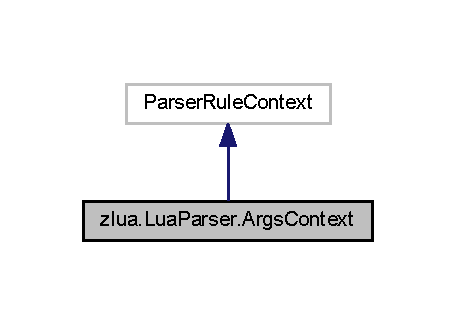
\includegraphics[width=219pt]{classzlua_1_1_lua_parser_1_1_args_context__inherit__graph}
\end{center}
\end{figure}


Collaboration diagram for zlua.\+Lua\+Parser.\+Args\+Context\+:
\nopagebreak
\begin{figure}[H]
\begin{center}
\leavevmode
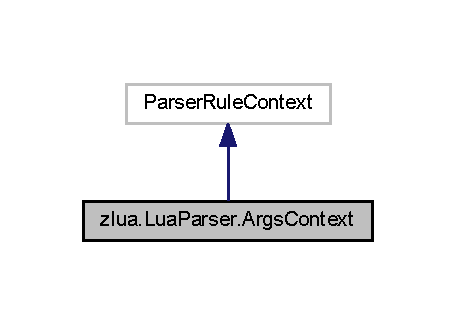
\includegraphics[width=219pt]{classzlua_1_1_lua_parser_1_1_args_context__coll__graph}
\end{center}
\end{figure}
\subsection*{Public Member Functions}
\begin{DoxyCompactItemize}
\item 
\mbox{\Hypertarget{classzlua_1_1_lua_parser_1_1_args_context_a9444177baf06bf0ae3bf2921a1530a3e}\label{classzlua_1_1_lua_parser_1_1_args_context_a9444177baf06bf0ae3bf2921a1530a3e}} 
\mbox{\hyperlink{classzlua_1_1_lua_parser_1_1_explist_context}{Explist\+Context}} {\bfseries explist} ()
\item 
\mbox{\Hypertarget{classzlua_1_1_lua_parser_1_1_args_context_acef19eec19b8b531ca47d4df5d9d3d66}\label{classzlua_1_1_lua_parser_1_1_args_context_acef19eec19b8b531ca47d4df5d9d3d66}} 
{\bfseries Args\+Context} (Parser\+Rule\+Context parent, int invoking\+State)
\item 
\mbox{\Hypertarget{classzlua_1_1_lua_parser_1_1_args_context_a6fe1916273abfa1d0232f74dacb2cc54}\label{classzlua_1_1_lua_parser_1_1_args_context_a6fe1916273abfa1d0232f74dacb2cc54}} 
override void {\bfseries Enter\+Rule} (I\+Parse\+Tree\+Listener listener)
\item 
\mbox{\Hypertarget{classzlua_1_1_lua_parser_1_1_args_context_a5d78b09eb2714e395ea448e7f3b0db24}\label{classzlua_1_1_lua_parser_1_1_args_context_a5d78b09eb2714e395ea448e7f3b0db24}} 
override void {\bfseries Exit\+Rule} (I\+Parse\+Tree\+Listener listener)
\item 
\mbox{\Hypertarget{classzlua_1_1_lua_parser_1_1_args_context_a41d43bd48fb04706781513e19ef6d79e}\label{classzlua_1_1_lua_parser_1_1_args_context_a41d43bd48fb04706781513e19ef6d79e}} 
override T\+Result {\bfseries Accept$<$ T\+Result $>$} (I\+Parse\+Tree\+Visitor$<$ T\+Result $>$ visitor)
\end{DoxyCompactItemize}
\subsection*{Properties}
\begin{DoxyCompactItemize}
\item 
\mbox{\Hypertarget{classzlua_1_1_lua_parser_1_1_args_context_a924a5f204e8b67d385a2bef5956b4e54}\label{classzlua_1_1_lua_parser_1_1_args_context_a924a5f204e8b67d385a2bef5956b4e54}} 
override int {\bfseries Rule\+Index}\hspace{0.3cm}{\ttfamily  \mbox{[}get\mbox{]}}
\end{DoxyCompactItemize}


The documentation for this class was generated from the following file\+:\begin{DoxyCompactItemize}
\item 
zlua/Lua\+Parser.\+cs\end{DoxyCompactItemize}

\hypertarget{classzlua_1_1_lua_1_1_assembled_instr}{}\section{zlua.\+Lua.\+Assembled\+Instr Class Reference}
\label{classzlua_1_1_lua_1_1_assembled_instr}\index{zlua.\+Lua.\+Assembled\+Instr@{zlua.\+Lua.\+Assembled\+Instr}}
\subsection*{Public Member Functions}
\begin{DoxyCompactItemize}
\item 
\mbox{\Hypertarget{classzlua_1_1_lua_1_1_assembled_instr_a2feea9c53ce8c484656ff5e4285cd74d}\label{classzlua_1_1_lua_1_1_assembled_instr_a2feea9c53ce8c484656ff5e4285cd74d}} 
override string {\bfseries To\+String} ()
\end{DoxyCompactItemize}


The documentation for this class was generated from the following file\+:\begin{DoxyCompactItemize}
\item 
zlua/lobject.\+cs\end{DoxyCompactItemize}

\hypertarget{classzlua_1_1_lua_parser_1_1_assign__stat_context}{}\section{zlua.\+Lua\+Parser.\+Assign\+\_\+stat\+Context Class Reference}
\label{classzlua_1_1_lua_parser_1_1_assign__stat_context}\index{zlua.\+Lua\+Parser.\+Assign\+\_\+stat\+Context@{zlua.\+Lua\+Parser.\+Assign\+\_\+stat\+Context}}


Inheritance diagram for zlua.\+Lua\+Parser.\+Assign\+\_\+stat\+Context\+:
\nopagebreak
\begin{figure}[H]
\begin{center}
\leavevmode
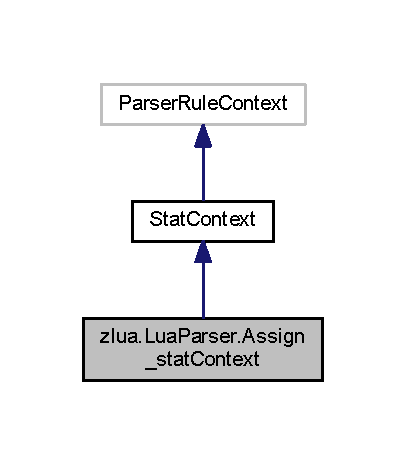
\includegraphics[width=195pt]{classzlua_1_1_lua_parser_1_1_assign__stat_context__inherit__graph}
\end{center}
\end{figure}


Collaboration diagram for zlua.\+Lua\+Parser.\+Assign\+\_\+stat\+Context\+:
\nopagebreak
\begin{figure}[H]
\begin{center}
\leavevmode
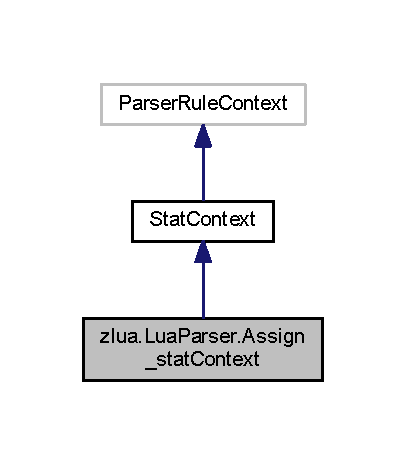
\includegraphics[width=195pt]{classzlua_1_1_lua_parser_1_1_assign__stat_context__coll__graph}
\end{center}
\end{figure}
\subsection*{Public Member Functions}
\begin{DoxyCompactItemize}
\item 
\mbox{\Hypertarget{classzlua_1_1_lua_parser_1_1_assign__stat_context_a60721a0facc985002939adddaefb531f}\label{classzlua_1_1_lua_parser_1_1_assign__stat_context_a60721a0facc985002939adddaefb531f}} 
\mbox{\hyperlink{classzlua_1_1_lua_parser_1_1_var_context}{Var\+Context}} {\bfseries var} ()
\item 
\mbox{\Hypertarget{classzlua_1_1_lua_parser_1_1_assign__stat_context_ac699ba21b9c4fb5905cf3685f1745418}\label{classzlua_1_1_lua_parser_1_1_assign__stat_context_ac699ba21b9c4fb5905cf3685f1745418}} 
\mbox{\hyperlink{classzlua_1_1_lua_parser_1_1_exp_context}{Exp\+Context}} {\bfseries exp} ()
\item 
\mbox{\Hypertarget{classzlua_1_1_lua_parser_1_1_assign__stat_context_a398dfb153417334b7945f9acadefcc90}\label{classzlua_1_1_lua_parser_1_1_assign__stat_context_a398dfb153417334b7945f9acadefcc90}} 
{\bfseries Assign\+\_\+stat\+Context} (\mbox{\hyperlink{classzlua_1_1_lua_parser_1_1_stat_context}{Stat\+Context}} context)
\item 
\mbox{\Hypertarget{classzlua_1_1_lua_parser_1_1_assign__stat_context_a124126deff881ab0cfd01d15e65827b4}\label{classzlua_1_1_lua_parser_1_1_assign__stat_context_a124126deff881ab0cfd01d15e65827b4}} 
override void {\bfseries Enter\+Rule} (I\+Parse\+Tree\+Listener listener)
\item 
\mbox{\Hypertarget{classzlua_1_1_lua_parser_1_1_assign__stat_context_a8fbb2a66611388da592a63c2ee7b55ba}\label{classzlua_1_1_lua_parser_1_1_assign__stat_context_a8fbb2a66611388da592a63c2ee7b55ba}} 
override void {\bfseries Exit\+Rule} (I\+Parse\+Tree\+Listener listener)
\item 
\mbox{\Hypertarget{classzlua_1_1_lua_parser_1_1_assign__stat_context_a55a5ccc6200ac036a2b93cb5ae6f7844}\label{classzlua_1_1_lua_parser_1_1_assign__stat_context_a55a5ccc6200ac036a2b93cb5ae6f7844}} 
override T\+Result {\bfseries Accept$<$ T\+Result $>$} (I\+Parse\+Tree\+Visitor$<$ T\+Result $>$ visitor)
\end{DoxyCompactItemize}
\subsection*{Additional Inherited Members}


The documentation for this class was generated from the following file\+:\begin{DoxyCompactItemize}
\item 
zlua/Lua\+Parser.\+cs\end{DoxyCompactItemize}

\hypertarget{classzlua_1_1_lua_parser_1_1_block_context}{}\section{zlua.\+Lua\+Parser.\+Block\+Context Class Reference}
\label{classzlua_1_1_lua_parser_1_1_block_context}\index{zlua.\+Lua\+Parser.\+Block\+Context@{zlua.\+Lua\+Parser.\+Block\+Context}}


Inheritance diagram for zlua.\+Lua\+Parser.\+Block\+Context\+:
\nopagebreak
\begin{figure}[H]
\begin{center}
\leavevmode
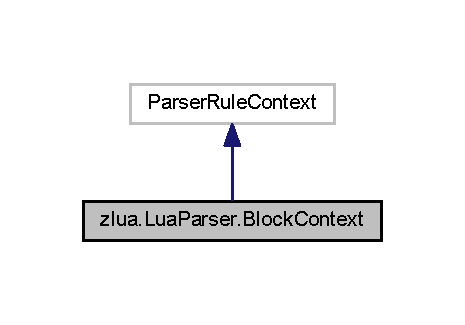
\includegraphics[width=223pt]{classzlua_1_1_lua_parser_1_1_block_context__inherit__graph}
\end{center}
\end{figure}


Collaboration diagram for zlua.\+Lua\+Parser.\+Block\+Context\+:
\nopagebreak
\begin{figure}[H]
\begin{center}
\leavevmode
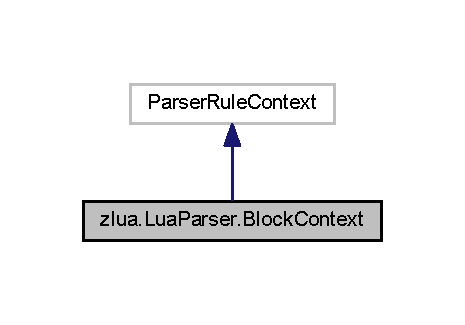
\includegraphics[width=223pt]{classzlua_1_1_lua_parser_1_1_block_context__coll__graph}
\end{center}
\end{figure}
\subsection*{Public Member Functions}
\begin{DoxyCompactItemize}
\item 
\mbox{\Hypertarget{classzlua_1_1_lua_parser_1_1_block_context_aefd87c6d742b9aedaeceaa3d49f17673}\label{classzlua_1_1_lua_parser_1_1_block_context_aefd87c6d742b9aedaeceaa3d49f17673}} 
\mbox{\hyperlink{classzlua_1_1_lua_parser_1_1_stat_context}{Stat\+Context}} \mbox{[}$\,$\mbox{]} {\bfseries stat} ()
\item 
\mbox{\Hypertarget{classzlua_1_1_lua_parser_1_1_block_context_a0c16e57fce5f61276d143739201f9c28}\label{classzlua_1_1_lua_parser_1_1_block_context_a0c16e57fce5f61276d143739201f9c28}} 
\mbox{\hyperlink{classzlua_1_1_lua_parser_1_1_stat_context}{Stat\+Context}} {\bfseries stat} (int i)
\item 
\mbox{\Hypertarget{classzlua_1_1_lua_parser_1_1_block_context_a7af7d7d934d9a9845758a61f203b63be}\label{classzlua_1_1_lua_parser_1_1_block_context_a7af7d7d934d9a9845758a61f203b63be}} 
\mbox{\hyperlink{classzlua_1_1_lua_parser_1_1_retstat_context}{Retstat\+Context}} {\bfseries retstat} ()
\item 
\mbox{\Hypertarget{classzlua_1_1_lua_parser_1_1_block_context_a460bade37efd71da8f467a0ac7ef9978}\label{classzlua_1_1_lua_parser_1_1_block_context_a460bade37efd71da8f467a0ac7ef9978}} 
{\bfseries Block\+Context} (Parser\+Rule\+Context parent, int invoking\+State)
\item 
\mbox{\Hypertarget{classzlua_1_1_lua_parser_1_1_block_context_a731bf8c6436a169c9803bc79d2030c55}\label{classzlua_1_1_lua_parser_1_1_block_context_a731bf8c6436a169c9803bc79d2030c55}} 
override void {\bfseries Enter\+Rule} (I\+Parse\+Tree\+Listener listener)
\item 
\mbox{\Hypertarget{classzlua_1_1_lua_parser_1_1_block_context_a9fd81c784c7bf1fdb7a8f4603f02ad9d}\label{classzlua_1_1_lua_parser_1_1_block_context_a9fd81c784c7bf1fdb7a8f4603f02ad9d}} 
override void {\bfseries Exit\+Rule} (I\+Parse\+Tree\+Listener listener)
\item 
\mbox{\Hypertarget{classzlua_1_1_lua_parser_1_1_block_context_a7bf3107ac797c02041d83083172c98b9}\label{classzlua_1_1_lua_parser_1_1_block_context_a7bf3107ac797c02041d83083172c98b9}} 
override T\+Result {\bfseries Accept$<$ T\+Result $>$} (I\+Parse\+Tree\+Visitor$<$ T\+Result $>$ visitor)
\end{DoxyCompactItemize}
\subsection*{Properties}
\begin{DoxyCompactItemize}
\item 
\mbox{\Hypertarget{classzlua_1_1_lua_parser_1_1_block_context_af3ae65d5ad2faf57315e634e9e4d1fd8}\label{classzlua_1_1_lua_parser_1_1_block_context_af3ae65d5ad2faf57315e634e9e4d1fd8}} 
override int {\bfseries Rule\+Index}\hspace{0.3cm}{\ttfamily  \mbox{[}get\mbox{]}}
\end{DoxyCompactItemize}


The documentation for this class was generated from the following file\+:\begin{DoxyCompactItemize}
\item 
zlua/Lua\+Parser.\+cs\end{DoxyCompactItemize}

\hypertarget{classzlua_1_1_lua_parser_1_1_break__stat_context}{}\section{zlua.\+Lua\+Parser.\+Break\+\_\+stat\+Context Class Reference}
\label{classzlua_1_1_lua_parser_1_1_break__stat_context}\index{zlua.\+Lua\+Parser.\+Break\+\_\+stat\+Context@{zlua.\+Lua\+Parser.\+Break\+\_\+stat\+Context}}


Inheritance diagram for zlua.\+Lua\+Parser.\+Break\+\_\+stat\+Context\+:
\nopagebreak
\begin{figure}[H]
\begin{center}
\leavevmode
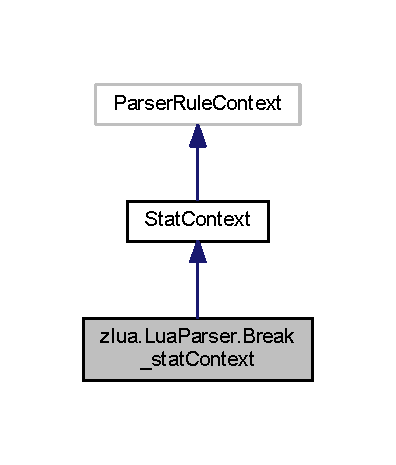
\includegraphics[width=190pt]{classzlua_1_1_lua_parser_1_1_break__stat_context__inherit__graph}
\end{center}
\end{figure}


Collaboration diagram for zlua.\+Lua\+Parser.\+Break\+\_\+stat\+Context\+:
\nopagebreak
\begin{figure}[H]
\begin{center}
\leavevmode
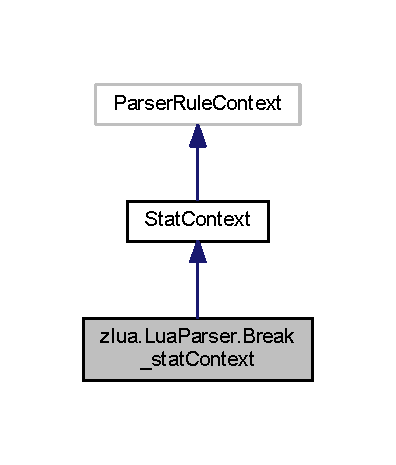
\includegraphics[width=190pt]{classzlua_1_1_lua_parser_1_1_break__stat_context__coll__graph}
\end{center}
\end{figure}
\subsection*{Public Member Functions}
\begin{DoxyCompactItemize}
\item 
\mbox{\Hypertarget{classzlua_1_1_lua_parser_1_1_break__stat_context_a1ec22ef954b90575779d51d2f122e4ee}\label{classzlua_1_1_lua_parser_1_1_break__stat_context_a1ec22ef954b90575779d51d2f122e4ee}} 
{\bfseries Break\+\_\+stat\+Context} (\mbox{\hyperlink{classzlua_1_1_lua_parser_1_1_stat_context}{Stat\+Context}} context)
\item 
\mbox{\Hypertarget{classzlua_1_1_lua_parser_1_1_break__stat_context_a3df65294faff6a2178b386fe21355be8}\label{classzlua_1_1_lua_parser_1_1_break__stat_context_a3df65294faff6a2178b386fe21355be8}} 
override void {\bfseries Enter\+Rule} (I\+Parse\+Tree\+Listener listener)
\item 
\mbox{\Hypertarget{classzlua_1_1_lua_parser_1_1_break__stat_context_ae76bf7f3afc33764f3573e6560416bb0}\label{classzlua_1_1_lua_parser_1_1_break__stat_context_ae76bf7f3afc33764f3573e6560416bb0}} 
override void {\bfseries Exit\+Rule} (I\+Parse\+Tree\+Listener listener)
\item 
\mbox{\Hypertarget{classzlua_1_1_lua_parser_1_1_break__stat_context_a9f8afb217e02f8ef7a4b3bf6021da125}\label{classzlua_1_1_lua_parser_1_1_break__stat_context_a9f8afb217e02f8ef7a4b3bf6021da125}} 
override T\+Result {\bfseries Accept$<$ T\+Result $>$} (I\+Parse\+Tree\+Visitor$<$ T\+Result $>$ visitor)
\end{DoxyCompactItemize}
\subsection*{Additional Inherited Members}


The documentation for this class was generated from the following file\+:\begin{DoxyCompactItemize}
\item 
zlua/Lua\+Parser.\+cs\end{DoxyCompactItemize}

\hypertarget{classzlua_1_1_lua_parser_1_1_chunk_context}{}\section{zlua.\+Lua\+Parser.\+Chunk\+Context Class Reference}
\label{classzlua_1_1_lua_parser_1_1_chunk_context}\index{zlua.\+Lua\+Parser.\+Chunk\+Context@{zlua.\+Lua\+Parser.\+Chunk\+Context}}


Inheritance diagram for zlua.\+Lua\+Parser.\+Chunk\+Context\+:
\nopagebreak
\begin{figure}[H]
\begin{center}
\leavevmode
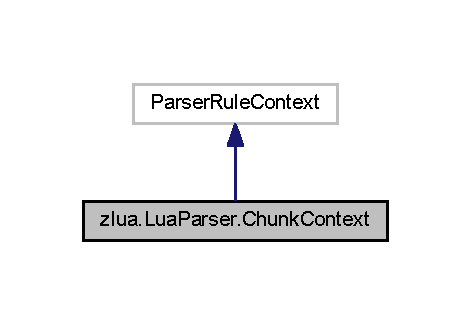
\includegraphics[width=226pt]{classzlua_1_1_lua_parser_1_1_chunk_context__inherit__graph}
\end{center}
\end{figure}


Collaboration diagram for zlua.\+Lua\+Parser.\+Chunk\+Context\+:
\nopagebreak
\begin{figure}[H]
\begin{center}
\leavevmode
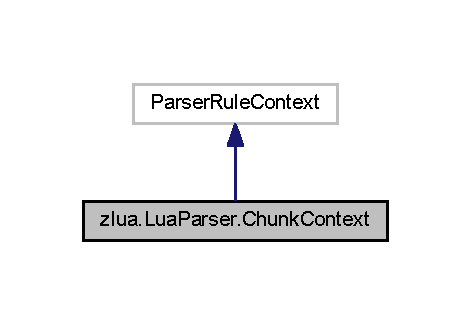
\includegraphics[width=226pt]{classzlua_1_1_lua_parser_1_1_chunk_context__coll__graph}
\end{center}
\end{figure}
\subsection*{Public Member Functions}
\begin{DoxyCompactItemize}
\item 
\mbox{\Hypertarget{classzlua_1_1_lua_parser_1_1_chunk_context_aac78cc34d1f6eb11e37283cab6bce0c7}\label{classzlua_1_1_lua_parser_1_1_chunk_context_aac78cc34d1f6eb11e37283cab6bce0c7}} 
\mbox{\hyperlink{classzlua_1_1_lua_parser_1_1_block_context}{Block\+Context}} {\bfseries block} ()
\item 
\mbox{\Hypertarget{classzlua_1_1_lua_parser_1_1_chunk_context_ab7f2bf8adfd2b279aeebc24ace4a31e2}\label{classzlua_1_1_lua_parser_1_1_chunk_context_ab7f2bf8adfd2b279aeebc24ace4a31e2}} 
I\+Terminal\+Node {\bfseries Eof} ()
\item 
\mbox{\Hypertarget{classzlua_1_1_lua_parser_1_1_chunk_context_adaa468f357b40c0182336c6fe4f237dc}\label{classzlua_1_1_lua_parser_1_1_chunk_context_adaa468f357b40c0182336c6fe4f237dc}} 
{\bfseries Chunk\+Context} (Parser\+Rule\+Context parent, int invoking\+State)
\item 
\mbox{\Hypertarget{classzlua_1_1_lua_parser_1_1_chunk_context_af1ddb755c62b1392d06bda6610f99e80}\label{classzlua_1_1_lua_parser_1_1_chunk_context_af1ddb755c62b1392d06bda6610f99e80}} 
override void {\bfseries Enter\+Rule} (I\+Parse\+Tree\+Listener listener)
\item 
\mbox{\Hypertarget{classzlua_1_1_lua_parser_1_1_chunk_context_acb91d70bdebaffe38769d683404dcdce}\label{classzlua_1_1_lua_parser_1_1_chunk_context_acb91d70bdebaffe38769d683404dcdce}} 
override void {\bfseries Exit\+Rule} (I\+Parse\+Tree\+Listener listener)
\item 
\mbox{\Hypertarget{classzlua_1_1_lua_parser_1_1_chunk_context_a2a03eda253da522b610c89fb100fde0c}\label{classzlua_1_1_lua_parser_1_1_chunk_context_a2a03eda253da522b610c89fb100fde0c}} 
override T\+Result {\bfseries Accept$<$ T\+Result $>$} (I\+Parse\+Tree\+Visitor$<$ T\+Result $>$ visitor)
\end{DoxyCompactItemize}
\subsection*{Properties}
\begin{DoxyCompactItemize}
\item 
\mbox{\Hypertarget{classzlua_1_1_lua_parser_1_1_chunk_context_a30940588ba9699051d60c4aa1038c7aa}\label{classzlua_1_1_lua_parser_1_1_chunk_context_a30940588ba9699051d60c4aa1038c7aa}} 
override int {\bfseries Rule\+Index}\hspace{0.3cm}{\ttfamily  \mbox{[}get\mbox{]}}
\end{DoxyCompactItemize}


The documentation for this class was generated from the following file\+:\begin{DoxyCompactItemize}
\item 
zlua/Lua\+Parser.\+cs\end{DoxyCompactItemize}

\hypertarget{classzlua_1_1_lua_1_1_compiled_function}{}\section{zlua.\+Lua.\+Compiled\+Function Class Reference}
\label{classzlua_1_1_lua_1_1_compiled_function}\index{zlua.\+Lua.\+Compiled\+Function@{zlua.\+Lua.\+Compiled\+Function}}


\char`\"{}\+Proto in lua.\+c\char`\"{} proto is gcobject, but is not a primitive type  




Inheritance diagram for zlua.\+Lua.\+Compiled\+Function\+:
\nopagebreak
\begin{figure}[H]
\begin{center}
\leavevmode
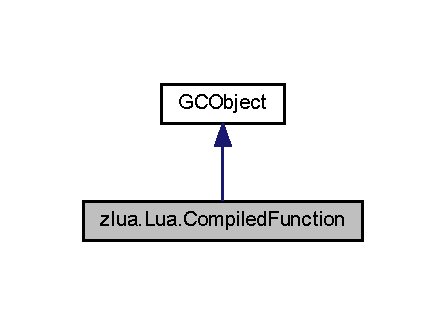
\includegraphics[width=214pt]{classzlua_1_1_lua_1_1_compiled_function__inherit__graph}
\end{center}
\end{figure}


Collaboration diagram for zlua.\+Lua.\+Compiled\+Function\+:
\nopagebreak
\begin{figure}[H]
\begin{center}
\leavevmode
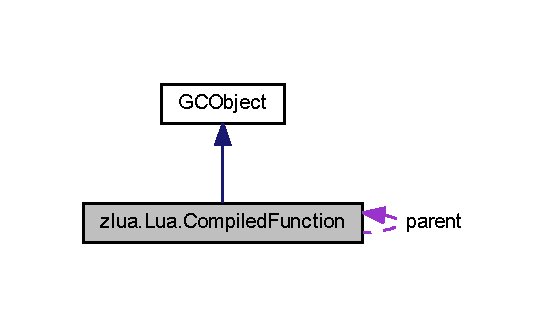
\includegraphics[width=263pt]{classzlua_1_1_lua_1_1_compiled_function__coll__graph}
\end{center}
\end{figure}
\subsection*{Public Attributes}
\begin{DoxyCompactItemize}
\item 
\mbox{\Hypertarget{classzlua_1_1_lua_1_1_compiled_function_aced124a626e6e66da9d2bbd03cb5cd1b}\label{classzlua_1_1_lua_1_1_compiled_function_aced124a626e6e66da9d2bbd03cb5cd1b}} 
List$<$ string $>$ {\bfseries param\+\_\+names}
\item 
\mbox{\Hypertarget{classzlua_1_1_lua_1_1_compiled_function_a5a2b11130a27a3efde8b41ffd07ee029}\label{classzlua_1_1_lua_1_1_compiled_function_a5a2b11130a27a3efde8b41ffd07ee029}} 
\mbox{\hyperlink{classzlua_1_1_lua_1_1_compiled_function}{Compiled\+Function}} {\bfseries parent}
\item 
\mbox{\Hypertarget{classzlua_1_1_lua_1_1_compiled_function_ab5740c8dbea8bd8b8439cd40f8b06151}\label{classzlua_1_1_lua_1_1_compiled_function_ab5740c8dbea8bd8b8439cd40f8b06151}} 
List$<$ \mbox{\hyperlink{classzlua_1_1_lua_1_1_assembled_instr}{Assembled\+Instr}} $>$ {\bfseries instrs}
\item 
\mbox{\Hypertarget{classzlua_1_1_lua_1_1_compiled_function_a4941bbbce70fa669ac532bc27b0ebe05}\label{classzlua_1_1_lua_1_1_compiled_function_a4941bbbce70fa669ac532bc27b0ebe05}} 
List$<$ \mbox{\hyperlink{classzlua_1_1_lua_1_1_compiled_function}{Compiled\+Function}} $>$ {\bfseries inner\+\_\+funcs}
\item 
\mbox{\Hypertarget{classzlua_1_1_lua_1_1_compiled_function_a76ab5e462e9c9f2d4236b19ec19403c3}\label{classzlua_1_1_lua_1_1_compiled_function_a76ab5e462e9c9f2d4236b19ec19403c3}} 
Dictionary$<$ string, int $>$ {\bfseries label2pc}
\end{DoxyCompactItemize}
\subsection*{Additional Inherited Members}


\subsection{Detailed Description}
\char`\"{}\+Proto in lua.\+c\char`\"{} proto is gcobject, but is not a primitive type 



The documentation for this class was generated from the following file\+:\begin{DoxyCompactItemize}
\item 
zlua/lobject.\+cs\end{DoxyCompactItemize}

\hypertarget{classzlua_1_1_compiler}{}\section{zlua.\+Compiler Class Reference}
\label{classzlua_1_1_compiler}\index{zlua.\+Compiler@{zlua.\+Compiler}}


Inheritance diagram for zlua.\+Compiler\+:
\nopagebreak
\begin{figure}[H]
\begin{center}
\leavevmode
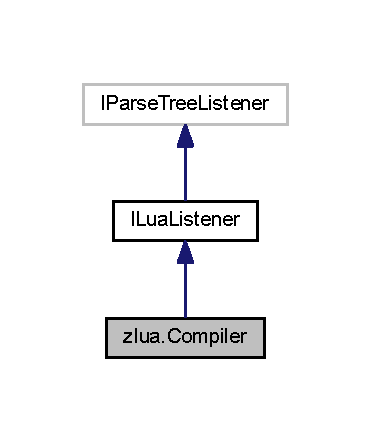
\includegraphics[width=178pt]{classzlua_1_1_compiler__inherit__graph}
\end{center}
\end{figure}


Collaboration diagram for zlua.\+Compiler\+:
\nopagebreak
\begin{figure}[H]
\begin{center}
\leavevmode
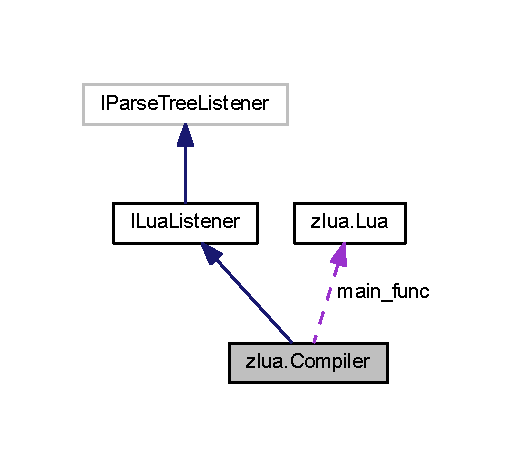
\includegraphics[width=247pt]{classzlua_1_1_compiler__coll__graph}
\end{center}
\end{figure}
\subsection*{Public Member Functions}
\begin{DoxyCompactItemize}
\item 
void \mbox{\hyperlink{classzlua_1_1_compiler_a60ee0650123807779b316af7cf7b213d}{Enter\+Args}} (\mbox{[}Not\+Null\mbox{]} \mbox{\hyperlink{classzlua_1_1_lua_parser_1_1_args_context}{Lua\+Parser.\+Args\+Context}} context)
\begin{DoxyCompactList}\small\item\em Enter a parse tree produced by Lua\+Parser.\+args. \end{DoxyCompactList}\item 
void \mbox{\hyperlink{classzlua_1_1_compiler_aaffd1a513f64fae2076a896a889e00bf}{Enter\+Assign\+\_\+stat}} (\mbox{[}Not\+Null\mbox{]} \mbox{\hyperlink{classzlua_1_1_lua_parser_1_1_assign__stat_context}{Lua\+Parser.\+Assign\+\_\+stat\+Context}} context)
\begin{DoxyCompactList}\small\item\em Enter a parse tree produced by the {\ttfamily assign\+\_\+stat} labeled alternative in Lua\+Parser.\+stat. \end{DoxyCompactList}\item 
void \mbox{\hyperlink{classzlua_1_1_compiler_a3bb0ad1158b35844611b3bbb75ff5521}{Enter\+Block}} (\mbox{[}Not\+Null\mbox{]} \mbox{\hyperlink{classzlua_1_1_lua_parser_1_1_block_context}{Lua\+Parser.\+Block\+Context}} context)
\begin{DoxyCompactList}\small\item\em Enter a parse tree produced by Lua\+Parser.\+block. \end{DoxyCompactList}\item 
void \mbox{\hyperlink{classzlua_1_1_compiler_afb51cc611219670d5372b0d22f1026a3}{Enter\+Break\+\_\+stat}} (\mbox{[}Not\+Null\mbox{]} \mbox{\hyperlink{classzlua_1_1_lua_parser_1_1_break__stat_context}{Lua\+Parser.\+Break\+\_\+stat\+Context}} context)
\begin{DoxyCompactList}\small\item\em Enter a parse tree produced by the {\ttfamily break\+\_\+stat} labeled alternative in Lua\+Parser.\+stat. \end{DoxyCompactList}\item 
void \mbox{\hyperlink{classzlua_1_1_compiler_ac52a396b2bba3e5b8767672a72593d79}{Enter\+Chunk}} (\mbox{[}Not\+Null\mbox{]} \mbox{\hyperlink{classzlua_1_1_lua_parser_1_1_chunk_context}{Lua\+Parser.\+Chunk\+Context}} context)
\begin{DoxyCompactList}\small\item\em Enter a parse tree produced by Lua\+Parser.\+chunk. \end{DoxyCompactList}\item 
void \mbox{\hyperlink{classzlua_1_1_compiler_a6995466e1f6349319b4b822ec3579e50}{Enter\+Do\+\_\+end\+\_\+stat}} (\mbox{[}Not\+Null\mbox{]} \mbox{\hyperlink{classzlua_1_1_lua_parser_1_1_do__end__stat_context}{Lua\+Parser.\+Do\+\_\+end\+\_\+stat\+Context}} context)
\begin{DoxyCompactList}\small\item\em Enter a parse tree produced by the {\ttfamily do\+\_\+end\+\_\+stat} labeled alternative in Lua\+Parser.\+stat. \end{DoxyCompactList}\item 
void \mbox{\hyperlink{classzlua_1_1_compiler_a56016ed91d28fe91587f18764fc23b1c}{Enter\+Empty\+\_\+stat}} (\mbox{[}Not\+Null\mbox{]} \mbox{\hyperlink{classzlua_1_1_lua_parser_1_1_empty__stat_context}{Lua\+Parser.\+Empty\+\_\+stat\+Context}} context)
\begin{DoxyCompactList}\small\item\em Enter a parse tree produced by the {\ttfamily empty\+\_\+stat} labeled alternative in Lua\+Parser.\+stat. \end{DoxyCompactList}\item 
\mbox{\Hypertarget{classzlua_1_1_compiler_a5b35e488ab7fa0289dd1b866c229601a}\label{classzlua_1_1_compiler_a5b35e488ab7fa0289dd1b866c229601a}} 
void {\bfseries Enter\+Every\+Rule} (Parser\+Rule\+Context ctx)
\item 
void \mbox{\hyperlink{classzlua_1_1_compiler_a602f2e28904cb93674d854f543cff30b}{Enter\+Exp}} (\mbox{[}Not\+Null\mbox{]} \mbox{\hyperlink{classzlua_1_1_lua_parser_1_1_exp_context}{Lua\+Parser.\+Exp\+Context}} context)
\begin{DoxyCompactList}\small\item\em Enter a parse tree produced by Lua\+Parser.\+exp. \end{DoxyCompactList}\item 
void \mbox{\hyperlink{classzlua_1_1_compiler_a1ae7390644425df6bdefe1b8d7d07ceb}{Enter\+Explist}} (\mbox{[}Not\+Null\mbox{]} \mbox{\hyperlink{classzlua_1_1_lua_parser_1_1_explist_context}{Lua\+Parser.\+Explist\+Context}} context)
\begin{DoxyCompactList}\small\item\em Enter a parse tree produced by Lua\+Parser.\+explist. \end{DoxyCompactList}\item 
void \mbox{\hyperlink{classzlua_1_1_compiler_a2679b9bd28b5726f5b1d45c391d44b1a}{Enter\+False\+\_\+exp}} (\mbox{[}Not\+Null\mbox{]} \mbox{\hyperlink{classzlua_1_1_lua_parser_1_1_false__exp_context}{Lua\+Parser.\+False\+\_\+exp\+Context}} context)
\begin{DoxyCompactList}\small\item\em Enter a parse tree produced by the {\ttfamily false\+\_\+exp} labeled alternative in Lua\+Parser.\+exp. \end{DoxyCompactList}\item 
void \mbox{\hyperlink{classzlua_1_1_compiler_a52a01acfde2fcb93cbec5f59549288da}{Enter\+Field}} (\mbox{[}Not\+Null\mbox{]} \mbox{\hyperlink{classzlua_1_1_lua_parser_1_1_field_context}{Lua\+Parser.\+Field\+Context}} context)
\begin{DoxyCompactList}\small\item\em Enter a parse tree produced by Lua\+Parser.\+field. \end{DoxyCompactList}\item 
void \mbox{\hyperlink{classzlua_1_1_compiler_a4f33b0f6f14a3497db13c22e4d03a10f}{Enter\+Fieldlist}} (\mbox{[}Not\+Null\mbox{]} \mbox{\hyperlink{classzlua_1_1_lua_parser_1_1_fieldlist_context}{Lua\+Parser.\+Fieldlist\+Context}} context)
\begin{DoxyCompactList}\small\item\em Enter a parse tree produced by Lua\+Parser.\+fieldlist. \end{DoxyCompactList}\item 
void \mbox{\hyperlink{classzlua_1_1_compiler_a4cd23e46335e41cd5c30ffae494efbec}{Enter\+Fieldsep}} (\mbox{[}Not\+Null\mbox{]} \mbox{\hyperlink{classzlua_1_1_lua_parser_1_1_fieldsep_context}{Lua\+Parser.\+Fieldsep\+Context}} context)
\begin{DoxyCompactList}\small\item\em Enter a parse tree produced by Lua\+Parser.\+fieldsep. \end{DoxyCompactList}\item 
void \mbox{\hyperlink{classzlua_1_1_compiler_a0ccbdaa518f36c6a9145c36adf12dd2e}{Enter\+Funcbody}} (\mbox{[}Not\+Null\mbox{]} \mbox{\hyperlink{classzlua_1_1_lua_parser_1_1_funcbody_context}{Lua\+Parser.\+Funcbody\+Context}} context)
\begin{DoxyCompactList}\small\item\em Enter a parse tree produced by Lua\+Parser.\+funcbody. \end{DoxyCompactList}\item 
void \mbox{\hyperlink{classzlua_1_1_compiler_a0da2d547d2333616052b776e192eaae5}{Enter\+Funcname}} (\mbox{[}Not\+Null\mbox{]} \mbox{\hyperlink{classzlua_1_1_lua_parser_1_1_funcname_context}{Lua\+Parser.\+Funcname\+Context}} context)
\begin{DoxyCompactList}\small\item\em Enter a parse tree produced by Lua\+Parser.\+funcname. \end{DoxyCompactList}\item 
void \mbox{\hyperlink{classzlua_1_1_compiler_a17169577cf49b4387d6f65f07354e370}{Enter\+Functioncall}} (\mbox{[}Not\+Null\mbox{]} \mbox{\hyperlink{classzlua_1_1_lua_parser_1_1_functioncall_context}{Lua\+Parser.\+Functioncall\+Context}} context)
\begin{DoxyCompactList}\small\item\em Enter a parse tree produced by Lua\+Parser.\+functioncall. \end{DoxyCompactList}\item 
void \mbox{\hyperlink{classzlua_1_1_compiler_a2e238ee43fa902a36201d2cae25375a1}{Enter\+Functiondef}} (\mbox{[}Not\+Null\mbox{]} \mbox{\hyperlink{classzlua_1_1_lua_parser_1_1_functiondef_context}{Lua\+Parser.\+Functiondef\+Context}} context)
\begin{DoxyCompactList}\small\item\em Enter a parse tree produced by Lua\+Parser.\+functiondef. \end{DoxyCompactList}\item 
void \mbox{\hyperlink{classzlua_1_1_compiler_a8a7c628a67d4fbca64f86739a32b1162}{Enter\+Func\+\_\+call\+\_\+stat}} (\mbox{[}Not\+Null\mbox{]} \mbox{\hyperlink{classzlua_1_1_lua_parser_1_1_func__call__stat_context}{Lua\+Parser.\+Func\+\_\+call\+\_\+stat\+Context}} context)
\begin{DoxyCompactList}\small\item\em Enter a parse tree produced by the {\ttfamily func\+\_\+call\+\_\+stat} labeled alternative in Lua\+Parser.\+stat. \end{DoxyCompactList}\item 
void \mbox{\hyperlink{classzlua_1_1_compiler_a626c3684acd46bdc1812ebd74d2ce10e}{Enter\+Func\+\_\+def\+\_\+exp}} (\mbox{[}Not\+Null\mbox{]} \mbox{\hyperlink{classzlua_1_1_lua_parser_1_1_func__def__exp_context}{Lua\+Parser.\+Func\+\_\+def\+\_\+exp\+Context}} context)
\begin{DoxyCompactList}\small\item\em Enter a parse tree produced by the {\ttfamily func\+\_\+def\+\_\+exp} labeled alternative in Lua\+Parser.\+exp. \end{DoxyCompactList}\item 
void \mbox{\hyperlink{classzlua_1_1_compiler_a2a2bdb04e6e4f416e0f6141c26981c3f}{Enter\+Func\+\_\+def\+\_\+stat}} (\mbox{[}Not\+Null\mbox{]} \mbox{\hyperlink{classzlua_1_1_lua_parser_1_1_func__def__stat_context}{Lua\+Parser.\+Func\+\_\+def\+\_\+stat\+Context}} context)
\begin{DoxyCompactList}\small\item\em Enter a parse tree produced by the {\ttfamily func\+\_\+def\+\_\+stat} labeled alternative in Lua\+Parser.\+stat. \end{DoxyCompactList}\item 
void \mbox{\hyperlink{classzlua_1_1_compiler_a895f16e966c211610d41e577ea359ed4}{Enter\+Global\+\_\+func\+\_\+def\+\_\+stat}} (\mbox{[}Not\+Null\mbox{]} \mbox{\hyperlink{classzlua_1_1_lua_parser_1_1_global__func__def__stat_context}{Lua\+Parser.\+Global\+\_\+func\+\_\+def\+\_\+stat\+Context}} context)
\begin{DoxyCompactList}\small\item\em Enter a parse tree produced by the {\ttfamily global\+\_\+func\+\_\+def\+\_\+stat} labeled alternative in Lua\+Parser.\+stat. \end{DoxyCompactList}\item 
void \mbox{\hyperlink{classzlua_1_1_compiler_a303b1c4d7a6cafe7c22c4ae4cdb2d296}{Enter\+Global\+\_\+var\+\_\+stat}} (\mbox{[}Not\+Null\mbox{]} \mbox{\hyperlink{classzlua_1_1_lua_parser_1_1_global__var__stat_context}{Lua\+Parser.\+Global\+\_\+var\+\_\+stat\+Context}} context)
\begin{DoxyCompactList}\small\item\em Enter a parse tree produced by the {\ttfamily global\+\_\+var\+\_\+stat} labeled alternative in Lua\+Parser.\+stat. \end{DoxyCompactList}\item 
void \mbox{\hyperlink{classzlua_1_1_compiler_af6ae77f24cf841b02733f92d10c21074}{Enter\+If\+\_\+stat}} (\mbox{[}Not\+Null\mbox{]} \mbox{\hyperlink{classzlua_1_1_lua_parser_1_1_if__stat_context}{Lua\+Parser.\+If\+\_\+stat\+Context}} context)
\begin{DoxyCompactList}\small\item\em Enter a parse tree produced by the {\ttfamily if\+\_\+stat} labeled alternative in Lua\+Parser.\+stat. \end{DoxyCompactList}\item 
void \mbox{\hyperlink{classzlua_1_1_compiler_a84d43624eeeff6bf6b9f229a8880fe0a}{Enter\+Name\+And\+Args}} (\mbox{[}Not\+Null\mbox{]} \mbox{\hyperlink{classzlua_1_1_lua_parser_1_1_name_and_args_context}{Lua\+Parser.\+Name\+And\+Args\+Context}} context)
\begin{DoxyCompactList}\small\item\em Enter a parse tree produced by Lua\+Parser.\+name\+And\+Args. \end{DoxyCompactList}\item 
void \mbox{\hyperlink{classzlua_1_1_compiler_a2a5054c21e462c7c373154ea435db694}{Enter\+Namelist}} (\mbox{[}Not\+Null\mbox{]} \mbox{\hyperlink{classzlua_1_1_lua_parser_1_1_namelist_context}{Lua\+Parser.\+Namelist\+Context}} context)
\begin{DoxyCompactList}\small\item\em Enter a parse tree produced by Lua\+Parser.\+namelist. \end{DoxyCompactList}\item 
void \mbox{\hyperlink{classzlua_1_1_compiler_a311aa04e7e5d26fae07d698a436dab6d}{Enter\+Nil\+\_\+exp}} (\mbox{[}Not\+Null\mbox{]} \mbox{\hyperlink{classzlua_1_1_lua_parser_1_1_nil__exp_context}{Lua\+Parser.\+Nil\+\_\+exp\+Context}} context)
\begin{DoxyCompactList}\small\item\em Enter a parse tree produced by the {\ttfamily nil\+\_\+exp} labeled alternative in Lua\+Parser.\+exp. \end{DoxyCompactList}\item 
void \mbox{\hyperlink{classzlua_1_1_compiler_a1bbda8fe66a0e085fa7b659d1690cda8}{Enter\+Number}} (\mbox{[}Not\+Null\mbox{]} \mbox{\hyperlink{classzlua_1_1_lua_parser_1_1_number_context}{Lua\+Parser.\+Number\+Context}} context)
\begin{DoxyCompactList}\small\item\em Enter a parse tree produced by Lua\+Parser.\+number. \end{DoxyCompactList}\item 
void \mbox{\hyperlink{classzlua_1_1_compiler_a8ef740c20e6771534630c1c897f0f2f4}{Enter\+Num\+\_\+exp}} (\mbox{[}Not\+Null\mbox{]} \mbox{\hyperlink{classzlua_1_1_lua_parser_1_1_num__exp_context}{Lua\+Parser.\+Num\+\_\+exp\+Context}} context)
\begin{DoxyCompactList}\small\item\em Enter a parse tree produced by the {\ttfamily num\+\_\+exp} labeled alternative in Lua\+Parser.\+exp. \end{DoxyCompactList}\item 
void \mbox{\hyperlink{classzlua_1_1_compiler_ad766e6d486cd81a33eca68f94ed7fb79}{Enter\+Operator\+Add\+Sub}} (\mbox{[}Not\+Null\mbox{]} \mbox{\hyperlink{classzlua_1_1_lua_parser_1_1_operator_add_sub_context}{Lua\+Parser.\+Operator\+Add\+Sub\+Context}} context)
\begin{DoxyCompactList}\small\item\em Enter a parse tree produced by Lua\+Parser.\+operator\+Add\+Sub. \end{DoxyCompactList}\item 
void \mbox{\hyperlink{classzlua_1_1_compiler_a028404702602498261a23021b36b5a87}{Enter\+Operator\+And}} (\mbox{[}Not\+Null\mbox{]} \mbox{\hyperlink{classzlua_1_1_lua_parser_1_1_operator_and_context}{Lua\+Parser.\+Operator\+And\+Context}} context)
\begin{DoxyCompactList}\small\item\em Enter a parse tree produced by Lua\+Parser.\+operator\+And. \end{DoxyCompactList}\item 
void \mbox{\hyperlink{classzlua_1_1_compiler_a13c55dd9aa0ccdf16a6855282091f63f}{Enter\+Operator\+Bitwise}} (\mbox{[}Not\+Null\mbox{]} \mbox{\hyperlink{classzlua_1_1_lua_parser_1_1_operator_bitwise_context}{Lua\+Parser.\+Operator\+Bitwise\+Context}} context)
\begin{DoxyCompactList}\small\item\em Enter a parse tree produced by Lua\+Parser.\+operator\+Bitwise. \end{DoxyCompactList}\item 
void \mbox{\hyperlink{classzlua_1_1_compiler_ac4a8baa233d08987d8f276972567c343}{Enter\+Operator\+Comparison}} (\mbox{[}Not\+Null\mbox{]} \mbox{\hyperlink{classzlua_1_1_lua_parser_1_1_operator_comparison_context}{Lua\+Parser.\+Operator\+Comparison\+Context}} context)
\begin{DoxyCompactList}\small\item\em Enter a parse tree produced by Lua\+Parser.\+operator\+Comparison. \end{DoxyCompactList}\item 
void \mbox{\hyperlink{classzlua_1_1_compiler_a59d6144f868523b34a542792c6dfafa2}{Enter\+Operator\+Mul\+Div\+Mod}} (\mbox{[}Not\+Null\mbox{]} \mbox{\hyperlink{classzlua_1_1_lua_parser_1_1_operator_mul_div_mod_context}{Lua\+Parser.\+Operator\+Mul\+Div\+Mod\+Context}} context)
\begin{DoxyCompactList}\small\item\em Enter a parse tree produced by Lua\+Parser.\+operator\+Mul\+Div\+Mod. \end{DoxyCompactList}\item 
void \mbox{\hyperlink{classzlua_1_1_compiler_a75f93e717dd16160d39907f826257579}{Enter\+Operator\+Or}} (\mbox{[}Not\+Null\mbox{]} \mbox{\hyperlink{classzlua_1_1_lua_parser_1_1_operator_or_context}{Lua\+Parser.\+Operator\+Or\+Context}} context)
\begin{DoxyCompactList}\small\item\em Enter a parse tree produced by Lua\+Parser.\+operator\+Or. \end{DoxyCompactList}\item 
void \mbox{\hyperlink{classzlua_1_1_compiler_a3e4509b5b2b44e581499d2264cf0e22f}{Enter\+Operator\+Power}} (\mbox{[}Not\+Null\mbox{]} \mbox{\hyperlink{classzlua_1_1_lua_parser_1_1_operator_power_context}{Lua\+Parser.\+Operator\+Power\+Context}} context)
\begin{DoxyCompactList}\small\item\em Enter a parse tree produced by Lua\+Parser.\+operator\+Power. \end{DoxyCompactList}\item 
void \mbox{\hyperlink{classzlua_1_1_compiler_a9e79fbc0bd20b36c90d0b53569a1f7d7}{Enter\+Operator\+Strcat}} (\mbox{[}Not\+Null\mbox{]} \mbox{\hyperlink{classzlua_1_1_lua_parser_1_1_operator_strcat_context}{Lua\+Parser.\+Operator\+Strcat\+Context}} context)
\begin{DoxyCompactList}\small\item\em Enter a parse tree produced by Lua\+Parser.\+operator\+Strcat. \end{DoxyCompactList}\item 
void \mbox{\hyperlink{classzlua_1_1_compiler_a1c085d48a4bc63b7b42cb8763f643bb2}{Enter\+Operator\+Unary}} (\mbox{[}Not\+Null\mbox{]} \mbox{\hyperlink{classzlua_1_1_lua_parser_1_1_operator_unary_context}{Lua\+Parser.\+Operator\+Unary\+Context}} context)
\begin{DoxyCompactList}\small\item\em Enter a parse tree produced by Lua\+Parser.\+operator\+Unary. \end{DoxyCompactList}\item 
void \mbox{\hyperlink{classzlua_1_1_compiler_abd725a31350fd6d1a132042ccda04b14}{Enter\+Op\+\_\+add\+\_\+sub\+\_\+exp}} (\mbox{[}Not\+Null\mbox{]} \mbox{\hyperlink{classzlua_1_1_lua_parser_1_1_op__add__sub__exp_context}{Lua\+Parser.\+Op\+\_\+add\+\_\+sub\+\_\+exp\+Context}} context)
\begin{DoxyCompactList}\small\item\em Enter a parse tree produced by the {\ttfamily op\+\_\+add\+\_\+sub\+\_\+exp} labeled alternative in Lua\+Parser.\+exp. \end{DoxyCompactList}\item 
void \mbox{\hyperlink{classzlua_1_1_compiler_a057cdeaef67ecf5a4d53ea10833b3d24}{Enter\+Op\+\_\+and\+\_\+exp}} (\mbox{[}Not\+Null\mbox{]} \mbox{\hyperlink{classzlua_1_1_lua_parser_1_1_op__and__exp_context}{Lua\+Parser.\+Op\+\_\+and\+\_\+exp\+Context}} context)
\begin{DoxyCompactList}\small\item\em Enter a parse tree produced by the {\ttfamily op\+\_\+and\+\_\+exp} labeled alternative in Lua\+Parser.\+exp. \end{DoxyCompactList}\item 
void \mbox{\hyperlink{classzlua_1_1_compiler_a3ee6eb43c518439f5e6df2496d4bd45f}{Enter\+Op\+\_\+caompare\+\_\+exp}} (\mbox{[}Not\+Null\mbox{]} \mbox{\hyperlink{classzlua_1_1_lua_parser_1_1_op__caompare__exp_context}{Lua\+Parser.\+Op\+\_\+caompare\+\_\+exp\+Context}} context)
\begin{DoxyCompactList}\small\item\em Enter a parse tree produced by the {\ttfamily op\+\_\+caompare\+\_\+exp} labeled alternative in Lua\+Parser.\+exp. \end{DoxyCompactList}\item 
void \mbox{\hyperlink{classzlua_1_1_compiler_ab34e6520919145a9c302e6847e8b36b7}{Enter\+Op\+\_\+concat\+\_\+exp}} (\mbox{[}Not\+Null\mbox{]} \mbox{\hyperlink{classzlua_1_1_lua_parser_1_1_op__concat__exp_context}{Lua\+Parser.\+Op\+\_\+concat\+\_\+exp\+Context}} context)
\begin{DoxyCompactList}\small\item\em Enter a parse tree produced by the {\ttfamily op\+\_\+concat\+\_\+exp} labeled alternative in Lua\+Parser.\+exp. \end{DoxyCompactList}\item 
void \mbox{\hyperlink{classzlua_1_1_compiler_ac79e4b2008ccb00f7209a5dbc9ce7362}{Enter\+Op\+\_\+mul\+\_\+div\+\_\+exp}} (\mbox{[}Not\+Null\mbox{]} \mbox{\hyperlink{classzlua_1_1_lua_parser_1_1_op__mul__div__exp_context}{Lua\+Parser.\+Op\+\_\+mul\+\_\+div\+\_\+exp\+Context}} context)
\begin{DoxyCompactList}\small\item\em Enter a parse tree produced by the {\ttfamily op\+\_\+mul\+\_\+div\+\_\+exp} labeled alternative in Lua\+Parser.\+exp. \end{DoxyCompactList}\item 
void \mbox{\hyperlink{classzlua_1_1_compiler_a00586a6ef587aa5305c9ab8071c15d5a}{Enter\+Op\+\_\+or\+\_\+exp}} (\mbox{[}Not\+Null\mbox{]} \mbox{\hyperlink{classzlua_1_1_lua_parser_1_1_op__or__exp_context}{Lua\+Parser.\+Op\+\_\+or\+\_\+exp\+Context}} context)
\begin{DoxyCompactList}\small\item\em Enter a parse tree produced by the {\ttfamily op\+\_\+or\+\_\+exp} labeled alternative in Lua\+Parser.\+exp. \end{DoxyCompactList}\item 
void \mbox{\hyperlink{classzlua_1_1_compiler_a6eb871aad9a35e90e75434308d7edac0}{Enter\+Op\+\_\+unary\+\_\+exp}} (\mbox{[}Not\+Null\mbox{]} \mbox{\hyperlink{classzlua_1_1_lua_parser_1_1_op__unary__exp_context}{Lua\+Parser.\+Op\+\_\+unary\+\_\+exp\+Context}} context)
\begin{DoxyCompactList}\small\item\em Enter a parse tree produced by the {\ttfamily op\+\_\+unary\+\_\+exp} labeled alternative in Lua\+Parser.\+exp. \end{DoxyCompactList}\item 
void \mbox{\hyperlink{classzlua_1_1_compiler_a6cca7cfa803b7be16090f38ffd6b7186}{Enter\+Parlist}} (\mbox{[}Not\+Null\mbox{]} \mbox{\hyperlink{classzlua_1_1_lua_parser_1_1_parlist_context}{Lua\+Parser.\+Parlist\+Context}} context)
\begin{DoxyCompactList}\small\item\em Enter a parse tree produced by Lua\+Parser.\+parlist. \end{DoxyCompactList}\item 
void \mbox{\hyperlink{classzlua_1_1_compiler_a275bfb29b3cb0fd2322f2a58d6de2e22}{Enter\+Prefixexp}} (\mbox{[}Not\+Null\mbox{]} \mbox{\hyperlink{classzlua_1_1_lua_parser_1_1_prefixexp_context}{Lua\+Parser.\+Prefixexp\+Context}} context)
\begin{DoxyCompactList}\small\item\em Enter a parse tree produced by Lua\+Parser.\+prefixexp. \end{DoxyCompactList}\item 
void \mbox{\hyperlink{classzlua_1_1_compiler_ad48048f780b0cb63ea44f0e45f26ddea}{Enter\+Prefix\+\_\+exp\+\_\+exp}} (\mbox{[}Not\+Null\mbox{]} \mbox{\hyperlink{classzlua_1_1_lua_parser_1_1_prefix__exp__exp_context}{Lua\+Parser.\+Prefix\+\_\+exp\+\_\+exp\+Context}} context)
\begin{DoxyCompactList}\small\item\em Enter a parse tree produced by the {\ttfamily prefix\+\_\+exp\+\_\+exp} labeled alternative in Lua\+Parser.\+exp. \end{DoxyCompactList}\item 
void \mbox{\hyperlink{classzlua_1_1_compiler_aee24dcb3e97d2fc95ec9c970867c8876}{Enter\+Retstat}} (\mbox{[}Not\+Null\mbox{]} \mbox{\hyperlink{classzlua_1_1_lua_parser_1_1_retstat_context}{Lua\+Parser.\+Retstat\+Context}} context)
\begin{DoxyCompactList}\small\item\em Enter a parse tree produced by Lua\+Parser.\+retstat. \end{DoxyCompactList}\item 
void \mbox{\hyperlink{classzlua_1_1_compiler_a5edb39400f408df076c2ac83554f08eb}{Enter\+Stat}} (\mbox{[}Not\+Null\mbox{]} \mbox{\hyperlink{classzlua_1_1_lua_parser_1_1_stat_context}{Lua\+Parser.\+Stat\+Context}} context)
\begin{DoxyCompactList}\small\item\em Enter a parse tree produced by Lua\+Parser.\+stat. \end{DoxyCompactList}\item 
void \mbox{\hyperlink{classzlua_1_1_compiler_a994696673f9c1c41e00d65b1e7bb1d39}{Enter\+String}} (\mbox{[}Not\+Null\mbox{]} \mbox{\hyperlink{classzlua_1_1_lua_parser_1_1_string_context}{Lua\+Parser.\+String\+Context}} context)
\begin{DoxyCompactList}\small\item\em Enter a parse tree produced by Lua\+Parser.\+string. \end{DoxyCompactList}\item 
void \mbox{\hyperlink{classzlua_1_1_compiler_aed4778e096225183ba6add21e832faaf}{Enter\+String\+\_\+exp}} (\mbox{[}Not\+Null\mbox{]} \mbox{\hyperlink{classzlua_1_1_lua_parser_1_1_string__exp_context}{Lua\+Parser.\+String\+\_\+exp\+Context}} context)
\begin{DoxyCompactList}\small\item\em Enter a parse tree produced by the {\ttfamily string\+\_\+exp} labeled alternative in Lua\+Parser.\+exp. \end{DoxyCompactList}\item 
void \mbox{\hyperlink{classzlua_1_1_compiler_af18957aed84481c7763b249286bd28b2}{Enter\+Tableconstructor}} (\mbox{[}Not\+Null\mbox{]} \mbox{\hyperlink{classzlua_1_1_lua_parser_1_1_tableconstructor_context}{Lua\+Parser.\+Tableconstructor\+Context}} context)
\begin{DoxyCompactList}\small\item\em Enter a parse tree produced by Lua\+Parser.\+tableconstructor. \end{DoxyCompactList}\item 
void \mbox{\hyperlink{classzlua_1_1_compiler_afbc0c7f12e4f12a6c032ce90cf17b2ef}{Enter\+Table\+\_\+ctor\+\_\+exp}} (\mbox{[}Not\+Null\mbox{]} \mbox{\hyperlink{classzlua_1_1_lua_parser_1_1_table__ctor__exp_context}{Lua\+Parser.\+Table\+\_\+ctor\+\_\+exp\+Context}} context)
\begin{DoxyCompactList}\small\item\em Enter a parse tree produced by the {\ttfamily table\+\_\+ctor\+\_\+exp} labeled alternative in Lua\+Parser.\+exp. \end{DoxyCompactList}\item 
void \mbox{\hyperlink{classzlua_1_1_compiler_acaa89ddcb610b21d92f1e3d574c678bf}{Enter\+True\+\_\+exp}} (\mbox{[}Not\+Null\mbox{]} \mbox{\hyperlink{classzlua_1_1_lua_parser_1_1_true__exp_context}{Lua\+Parser.\+True\+\_\+exp\+Context}} context)
\begin{DoxyCompactList}\small\item\em Enter a parse tree produced by the {\ttfamily true\+\_\+exp} labeled alternative in Lua\+Parser.\+exp. \end{DoxyCompactList}\item 
void \mbox{\hyperlink{classzlua_1_1_compiler_aa81e525edf991e9e6a3e391814d449fe}{Enter\+Var}} (\mbox{[}Not\+Null\mbox{]} \mbox{\hyperlink{classzlua_1_1_lua_parser_1_1_var_context}{Lua\+Parser.\+Var\+Context}} context)
\begin{DoxyCompactList}\small\item\em Enter a parse tree produced by Lua\+Parser.\+var. \end{DoxyCompactList}\item 
void \mbox{\hyperlink{classzlua_1_1_compiler_ad7137ae6c666bc8dedb3cd24c8b22c49}{Enter\+Varlist}} (\mbox{[}Not\+Null\mbox{]} \mbox{\hyperlink{classzlua_1_1_lua_parser_1_1_varlist_context}{Lua\+Parser.\+Varlist\+Context}} context)
\begin{DoxyCompactList}\small\item\em Enter a parse tree produced by Lua\+Parser.\+varlist. \end{DoxyCompactList}\item 
void \mbox{\hyperlink{classzlua_1_1_compiler_ab7d4a2ccfca5f520e9702eaccab9872b}{Enter\+Var\+Or\+Exp}} (\mbox{[}Not\+Null\mbox{]} \mbox{\hyperlink{classzlua_1_1_lua_parser_1_1_var_or_exp_context}{Lua\+Parser.\+Var\+Or\+Exp\+Context}} context)
\begin{DoxyCompactList}\small\item\em Enter a parse tree produced by Lua\+Parser.\+var\+Or\+Exp. \end{DoxyCompactList}\item 
void \mbox{\hyperlink{classzlua_1_1_compiler_a6d026840f7eb9bbbdbc9b279c5929e86}{Enter\+Var\+Suffix}} (\mbox{[}Not\+Null\mbox{]} \mbox{\hyperlink{classzlua_1_1_lua_parser_1_1_var_suffix_context}{Lua\+Parser.\+Var\+Suffix\+Context}} context)
\begin{DoxyCompactList}\small\item\em Enter a parse tree produced by Lua\+Parser.\+var\+Suffix. \end{DoxyCompactList}\item 
void \mbox{\hyperlink{classzlua_1_1_compiler_a353452b5dbe912d06c08a6429be95906}{Enter\+While\+\_\+stat}} (\mbox{[}Not\+Null\mbox{]} \mbox{\hyperlink{classzlua_1_1_lua_parser_1_1_while__stat_context}{Lua\+Parser.\+While\+\_\+stat\+Context}} context)
\begin{DoxyCompactList}\small\item\em Enter a parse tree produced by the {\ttfamily while\+\_\+stat} labeled alternative in Lua\+Parser.\+stat. \end{DoxyCompactList}\item 
void \mbox{\hyperlink{classzlua_1_1_compiler_ae35672ab6cc512e4dab4ddc9063d9f22}{Exit\+Args}} (\mbox{[}Not\+Null\mbox{]} \mbox{\hyperlink{classzlua_1_1_lua_parser_1_1_args_context}{Lua\+Parser.\+Args\+Context}} context)
\begin{DoxyCompactList}\small\item\em Exit a parse tree produced by Lua\+Parser.\+args. \end{DoxyCompactList}\item 
void \mbox{\hyperlink{classzlua_1_1_compiler_a122e9a6b8770d627e6461baee20fcf62}{Exit\+Assign\+\_\+stat}} (\mbox{[}Not\+Null\mbox{]} \mbox{\hyperlink{classzlua_1_1_lua_parser_1_1_assign__stat_context}{Lua\+Parser.\+Assign\+\_\+stat\+Context}} context)
\begin{DoxyCompactList}\small\item\em Exit a parse tree produced by the {\ttfamily assign\+\_\+stat} labeled alternative in Lua\+Parser.\+stat. \end{DoxyCompactList}\item 
void \mbox{\hyperlink{classzlua_1_1_compiler_a75376c8d84a2bb594e2fab53270000fb}{Exit\+Block}} (\mbox{[}Not\+Null\mbox{]} \mbox{\hyperlink{classzlua_1_1_lua_parser_1_1_block_context}{Lua\+Parser.\+Block\+Context}} context)
\begin{DoxyCompactList}\small\item\em Exit a parse tree produced by Lua\+Parser.\+block. \end{DoxyCompactList}\item 
void \mbox{\hyperlink{classzlua_1_1_compiler_a6d60d0ca6f6c6c85d7ed31f0e7e8514d}{Exit\+Break\+\_\+stat}} (\mbox{[}Not\+Null\mbox{]} \mbox{\hyperlink{classzlua_1_1_lua_parser_1_1_break__stat_context}{Lua\+Parser.\+Break\+\_\+stat\+Context}} context)
\begin{DoxyCompactList}\small\item\em Exit a parse tree produced by the {\ttfamily break\+\_\+stat} labeled alternative in Lua\+Parser.\+stat. \end{DoxyCompactList}\item 
void \mbox{\hyperlink{classzlua_1_1_compiler_a1f313aa9552acb3fa730ac091a4fa17d}{Exit\+Chunk}} (\mbox{[}Not\+Null\mbox{]} \mbox{\hyperlink{classzlua_1_1_lua_parser_1_1_chunk_context}{Lua\+Parser.\+Chunk\+Context}} context)
\begin{DoxyCompactList}\small\item\em Exit a parse tree produced by Lua\+Parser.\+chunk. \end{DoxyCompactList}\item 
void \mbox{\hyperlink{classzlua_1_1_compiler_aaad82853d1a4a26480b3ae56adbc58f6}{Exit\+Do\+\_\+end\+\_\+stat}} (\mbox{[}Not\+Null\mbox{]} \mbox{\hyperlink{classzlua_1_1_lua_parser_1_1_do__end__stat_context}{Lua\+Parser.\+Do\+\_\+end\+\_\+stat\+Context}} context)
\begin{DoxyCompactList}\small\item\em Exit a parse tree produced by the {\ttfamily do\+\_\+end\+\_\+stat} labeled alternative in Lua\+Parser.\+stat. \end{DoxyCompactList}\item 
void \mbox{\hyperlink{classzlua_1_1_compiler_a6e35167b78ef83dd011df22f00c919a9}{Exit\+Empty\+\_\+stat}} (\mbox{[}Not\+Null\mbox{]} \mbox{\hyperlink{classzlua_1_1_lua_parser_1_1_empty__stat_context}{Lua\+Parser.\+Empty\+\_\+stat\+Context}} context)
\begin{DoxyCompactList}\small\item\em Exit a parse tree produced by the {\ttfamily empty\+\_\+stat} labeled alternative in Lua\+Parser.\+stat. \end{DoxyCompactList}\item 
\mbox{\Hypertarget{classzlua_1_1_compiler_ac0666696d34abc866e65101d6c7484e8}\label{classzlua_1_1_compiler_ac0666696d34abc866e65101d6c7484e8}} 
void {\bfseries Exit\+Every\+Rule} (Parser\+Rule\+Context ctx)
\item 
void \mbox{\hyperlink{classzlua_1_1_compiler_afab9279bd386382fb1fa91044f5b8e71}{Exit\+Exp}} (\mbox{[}Not\+Null\mbox{]} \mbox{\hyperlink{classzlua_1_1_lua_parser_1_1_exp_context}{Lua\+Parser.\+Exp\+Context}} context)
\begin{DoxyCompactList}\small\item\em Exit a parse tree produced by Lua\+Parser.\+exp. \end{DoxyCompactList}\item 
void \mbox{\hyperlink{classzlua_1_1_compiler_a54d71e09af5891553fa884334ce40a14}{Exit\+Explist}} (\mbox{[}Not\+Null\mbox{]} \mbox{\hyperlink{classzlua_1_1_lua_parser_1_1_explist_context}{Lua\+Parser.\+Explist\+Context}} context)
\begin{DoxyCompactList}\small\item\em Exit a parse tree produced by Lua\+Parser.\+explist. \end{DoxyCompactList}\item 
void \mbox{\hyperlink{classzlua_1_1_compiler_a0e5e286cdb08d9d9ef551f10f4447cf4}{Exit\+False\+\_\+exp}} (\mbox{[}Not\+Null\mbox{]} \mbox{\hyperlink{classzlua_1_1_lua_parser_1_1_false__exp_context}{Lua\+Parser.\+False\+\_\+exp\+Context}} context)
\begin{DoxyCompactList}\small\item\em Exit a parse tree produced by the {\ttfamily false\+\_\+exp} labeled alternative in Lua\+Parser.\+exp. \end{DoxyCompactList}\item 
void \mbox{\hyperlink{classzlua_1_1_compiler_a169d31b8bd893ddc06b90184f76ecdc7}{Exit\+Field}} (\mbox{[}Not\+Null\mbox{]} \mbox{\hyperlink{classzlua_1_1_lua_parser_1_1_field_context}{Lua\+Parser.\+Field\+Context}} context)
\begin{DoxyCompactList}\small\item\em Exit a parse tree produced by Lua\+Parser.\+field. \end{DoxyCompactList}\item 
void \mbox{\hyperlink{classzlua_1_1_compiler_abff740fa28ffb3a5dfd363aff46825b1}{Exit\+Fieldlist}} (\mbox{[}Not\+Null\mbox{]} \mbox{\hyperlink{classzlua_1_1_lua_parser_1_1_fieldlist_context}{Lua\+Parser.\+Fieldlist\+Context}} context)
\begin{DoxyCompactList}\small\item\em Exit a parse tree produced by Lua\+Parser.\+fieldlist. \end{DoxyCompactList}\item 
void \mbox{\hyperlink{classzlua_1_1_compiler_a7a8e74fbfd05fe67a5f51db87236b3e8}{Exit\+Fieldsep}} (\mbox{[}Not\+Null\mbox{]} \mbox{\hyperlink{classzlua_1_1_lua_parser_1_1_fieldsep_context}{Lua\+Parser.\+Fieldsep\+Context}} context)
\begin{DoxyCompactList}\small\item\em Exit a parse tree produced by Lua\+Parser.\+fieldsep. \end{DoxyCompactList}\item 
void \mbox{\hyperlink{classzlua_1_1_compiler_a42142f05b01646d0b407f241fd406939}{Exit\+Funcbody}} (\mbox{[}Not\+Null\mbox{]} \mbox{\hyperlink{classzlua_1_1_lua_parser_1_1_funcbody_context}{Lua\+Parser.\+Funcbody\+Context}} context)
\begin{DoxyCompactList}\small\item\em Exit a parse tree produced by Lua\+Parser.\+funcbody. \end{DoxyCompactList}\item 
void \mbox{\hyperlink{classzlua_1_1_compiler_adc2ed4db7299eb84e5a16cdbcda257d4}{Exit\+Funcname}} (\mbox{[}Not\+Null\mbox{]} \mbox{\hyperlink{classzlua_1_1_lua_parser_1_1_funcname_context}{Lua\+Parser.\+Funcname\+Context}} context)
\begin{DoxyCompactList}\small\item\em Exit a parse tree produced by Lua\+Parser.\+funcname. \end{DoxyCompactList}\item 
void \mbox{\hyperlink{classzlua_1_1_compiler_add5efa354ab9c4c04eb03d835b697acc}{Exit\+Functioncall}} (\mbox{[}Not\+Null\mbox{]} \mbox{\hyperlink{classzlua_1_1_lua_parser_1_1_functioncall_context}{Lua\+Parser.\+Functioncall\+Context}} context)
\begin{DoxyCompactList}\small\item\em Exit a parse tree produced by Lua\+Parser.\+functioncall. \end{DoxyCompactList}\item 
void \mbox{\hyperlink{classzlua_1_1_compiler_ac116526982cb40d063ff68949ab001e0}{Exit\+Functiondef}} (\mbox{[}Not\+Null\mbox{]} \mbox{\hyperlink{classzlua_1_1_lua_parser_1_1_functiondef_context}{Lua\+Parser.\+Functiondef\+Context}} context)
\begin{DoxyCompactList}\small\item\em Exit a parse tree produced by Lua\+Parser.\+functiondef. \end{DoxyCompactList}\item 
void \mbox{\hyperlink{classzlua_1_1_compiler_aecbd4798190717227c32cbd132d996dd}{Exit\+Func\+\_\+call\+\_\+stat}} (\mbox{[}Not\+Null\mbox{]} \mbox{\hyperlink{classzlua_1_1_lua_parser_1_1_func__call__stat_context}{Lua\+Parser.\+Func\+\_\+call\+\_\+stat\+Context}} context)
\begin{DoxyCompactList}\small\item\em Exit a parse tree produced by the {\ttfamily func\+\_\+call\+\_\+stat} labeled alternative in Lua\+Parser.\+stat. \end{DoxyCompactList}\item 
void \mbox{\hyperlink{classzlua_1_1_compiler_a52eac177380013cc2c8751c4bee9d1dc}{Exit\+Func\+\_\+def\+\_\+exp}} (\mbox{[}Not\+Null\mbox{]} \mbox{\hyperlink{classzlua_1_1_lua_parser_1_1_func__def__exp_context}{Lua\+Parser.\+Func\+\_\+def\+\_\+exp\+Context}} context)
\begin{DoxyCompactList}\small\item\em Exit a parse tree produced by the {\ttfamily func\+\_\+def\+\_\+exp} labeled alternative in Lua\+Parser.\+exp. \end{DoxyCompactList}\item 
void \mbox{\hyperlink{classzlua_1_1_compiler_a3c652ebce04bd5127161319606311859}{Exit\+Func\+\_\+def\+\_\+stat}} (\mbox{[}Not\+Null\mbox{]} \mbox{\hyperlink{classzlua_1_1_lua_parser_1_1_func__def__stat_context}{Lua\+Parser.\+Func\+\_\+def\+\_\+stat\+Context}} context)
\begin{DoxyCompactList}\small\item\em Exit a parse tree produced by the {\ttfamily func\+\_\+def\+\_\+stat} labeled alternative in Lua\+Parser.\+stat. \end{DoxyCompactList}\item 
void \mbox{\hyperlink{classzlua_1_1_compiler_a2d4b742668c3002d6396dca636a97dce}{Exit\+Global\+\_\+func\+\_\+def\+\_\+stat}} (\mbox{[}Not\+Null\mbox{]} \mbox{\hyperlink{classzlua_1_1_lua_parser_1_1_global__func__def__stat_context}{Lua\+Parser.\+Global\+\_\+func\+\_\+def\+\_\+stat\+Context}} context)
\begin{DoxyCompactList}\small\item\em Exit a parse tree produced by the {\ttfamily global\+\_\+func\+\_\+def\+\_\+stat} labeled alternative in Lua\+Parser.\+stat. \end{DoxyCompactList}\item 
void \mbox{\hyperlink{classzlua_1_1_compiler_a6c1f448ee93660853921f2c0048bc173}{Exit\+Global\+\_\+var\+\_\+stat}} (\mbox{[}Not\+Null\mbox{]} \mbox{\hyperlink{classzlua_1_1_lua_parser_1_1_global__var__stat_context}{Lua\+Parser.\+Global\+\_\+var\+\_\+stat\+Context}} context)
\begin{DoxyCompactList}\small\item\em Exit a parse tree produced by the {\ttfamily global\+\_\+var\+\_\+stat} labeled alternative in Lua\+Parser.\+stat. \end{DoxyCompactList}\item 
void \mbox{\hyperlink{classzlua_1_1_compiler_afca7da08ee84a7b0797de722420b443a}{Exit\+If\+\_\+stat}} (\mbox{[}Not\+Null\mbox{]} \mbox{\hyperlink{classzlua_1_1_lua_parser_1_1_if__stat_context}{Lua\+Parser.\+If\+\_\+stat\+Context}} context)
\begin{DoxyCompactList}\small\item\em Exit a parse tree produced by the {\ttfamily if\+\_\+stat} labeled alternative in Lua\+Parser.\+stat. \end{DoxyCompactList}\item 
void \mbox{\hyperlink{classzlua_1_1_compiler_afa2dba6f3e7fb7b060741a58bdac97f4}{Exit\+Name\+And\+Args}} (\mbox{[}Not\+Null\mbox{]} \mbox{\hyperlink{classzlua_1_1_lua_parser_1_1_name_and_args_context}{Lua\+Parser.\+Name\+And\+Args\+Context}} context)
\begin{DoxyCompactList}\small\item\em Exit a parse tree produced by Lua\+Parser.\+name\+And\+Args. \end{DoxyCompactList}\item 
void \mbox{\hyperlink{classzlua_1_1_compiler_ad35fb734ce46c317f3d6005186ff5a11}{Exit\+Namelist}} (\mbox{[}Not\+Null\mbox{]} \mbox{\hyperlink{classzlua_1_1_lua_parser_1_1_namelist_context}{Lua\+Parser.\+Namelist\+Context}} context)
\begin{DoxyCompactList}\small\item\em Exit a parse tree produced by Lua\+Parser.\+namelist. \end{DoxyCompactList}\item 
void \mbox{\hyperlink{classzlua_1_1_compiler_a1ec231e95547be0d28e8d1f30f4872ba}{Exit\+Nil\+\_\+exp}} (\mbox{[}Not\+Null\mbox{]} \mbox{\hyperlink{classzlua_1_1_lua_parser_1_1_nil__exp_context}{Lua\+Parser.\+Nil\+\_\+exp\+Context}} context)
\begin{DoxyCompactList}\small\item\em Exit a parse tree produced by the {\ttfamily nil\+\_\+exp} labeled alternative in Lua\+Parser.\+exp. \end{DoxyCompactList}\item 
void \mbox{\hyperlink{classzlua_1_1_compiler_a89a20cafde0ae8bc4079c91635b47c5f}{Exit\+Number}} (\mbox{[}Not\+Null\mbox{]} \mbox{\hyperlink{classzlua_1_1_lua_parser_1_1_number_context}{Lua\+Parser.\+Number\+Context}} context)
\begin{DoxyCompactList}\small\item\em Exit a parse tree produced by Lua\+Parser.\+number. \end{DoxyCompactList}\item 
void \mbox{\hyperlink{classzlua_1_1_compiler_a3a76d8ff765978e61655469c1277c65e}{Exit\+Num\+\_\+exp}} (\mbox{[}Not\+Null\mbox{]} \mbox{\hyperlink{classzlua_1_1_lua_parser_1_1_num__exp_context}{Lua\+Parser.\+Num\+\_\+exp\+Context}} context)
\begin{DoxyCompactList}\small\item\em Exit a parse tree produced by the {\ttfamily num\+\_\+exp} labeled alternative in Lua\+Parser.\+exp. \end{DoxyCompactList}\item 
void \mbox{\hyperlink{classzlua_1_1_compiler_a1559fa97735e564dc0cc25c6c5ec355a}{Exit\+Operator\+Add\+Sub}} (\mbox{[}Not\+Null\mbox{]} \mbox{\hyperlink{classzlua_1_1_lua_parser_1_1_operator_add_sub_context}{Lua\+Parser.\+Operator\+Add\+Sub\+Context}} context)
\begin{DoxyCompactList}\small\item\em Exit a parse tree produced by Lua\+Parser.\+operator\+Add\+Sub. \end{DoxyCompactList}\item 
void \mbox{\hyperlink{classzlua_1_1_compiler_a57e026e3b4f6ec40d78cc9f4c8068ad3}{Exit\+Operator\+And}} (\mbox{[}Not\+Null\mbox{]} \mbox{\hyperlink{classzlua_1_1_lua_parser_1_1_operator_and_context}{Lua\+Parser.\+Operator\+And\+Context}} context)
\begin{DoxyCompactList}\small\item\em Exit a parse tree produced by Lua\+Parser.\+operator\+And. \end{DoxyCompactList}\item 
void \mbox{\hyperlink{classzlua_1_1_compiler_ac96911516696a03a45807348f6338b41}{Exit\+Operator\+Bitwise}} (\mbox{[}Not\+Null\mbox{]} \mbox{\hyperlink{classzlua_1_1_lua_parser_1_1_operator_bitwise_context}{Lua\+Parser.\+Operator\+Bitwise\+Context}} context)
\begin{DoxyCompactList}\small\item\em Exit a parse tree produced by Lua\+Parser.\+operator\+Bitwise. \end{DoxyCompactList}\item 
void \mbox{\hyperlink{classzlua_1_1_compiler_af08a21dc48be4131cee4560b260d09c2}{Exit\+Operator\+Comparison}} (\mbox{[}Not\+Null\mbox{]} \mbox{\hyperlink{classzlua_1_1_lua_parser_1_1_operator_comparison_context}{Lua\+Parser.\+Operator\+Comparison\+Context}} context)
\begin{DoxyCompactList}\small\item\em Exit a parse tree produced by Lua\+Parser.\+operator\+Comparison. \end{DoxyCompactList}\item 
void \mbox{\hyperlink{classzlua_1_1_compiler_ab995afb210e4d04b7ebdcdd62f8f1541}{Exit\+Operator\+Mul\+Div\+Mod}} (\mbox{[}Not\+Null\mbox{]} \mbox{\hyperlink{classzlua_1_1_lua_parser_1_1_operator_mul_div_mod_context}{Lua\+Parser.\+Operator\+Mul\+Div\+Mod\+Context}} context)
\begin{DoxyCompactList}\small\item\em Exit a parse tree produced by Lua\+Parser.\+operator\+Mul\+Div\+Mod. \end{DoxyCompactList}\item 
void \mbox{\hyperlink{classzlua_1_1_compiler_a51d355ddfa730787d5353559db7acbce}{Exit\+Operator\+Or}} (\mbox{[}Not\+Null\mbox{]} \mbox{\hyperlink{classzlua_1_1_lua_parser_1_1_operator_or_context}{Lua\+Parser.\+Operator\+Or\+Context}} context)
\begin{DoxyCompactList}\small\item\em Exit a parse tree produced by Lua\+Parser.\+operator\+Or. \end{DoxyCompactList}\item 
void \mbox{\hyperlink{classzlua_1_1_compiler_a5c623270aa4a3005cf103f95ff8566a7}{Exit\+Operator\+Power}} (\mbox{[}Not\+Null\mbox{]} \mbox{\hyperlink{classzlua_1_1_lua_parser_1_1_operator_power_context}{Lua\+Parser.\+Operator\+Power\+Context}} context)
\begin{DoxyCompactList}\small\item\em Exit a parse tree produced by Lua\+Parser.\+operator\+Power. \end{DoxyCompactList}\item 
void \mbox{\hyperlink{classzlua_1_1_compiler_a320c32704688e1ba4705eb347b0e5701}{Exit\+Operator\+Strcat}} (\mbox{[}Not\+Null\mbox{]} \mbox{\hyperlink{classzlua_1_1_lua_parser_1_1_operator_strcat_context}{Lua\+Parser.\+Operator\+Strcat\+Context}} context)
\begin{DoxyCompactList}\small\item\em Exit a parse tree produced by Lua\+Parser.\+operator\+Strcat. \end{DoxyCompactList}\item 
void \mbox{\hyperlink{classzlua_1_1_compiler_a345eb068591d3ef3beddc652b206e53f}{Exit\+Operator\+Unary}} (\mbox{[}Not\+Null\mbox{]} \mbox{\hyperlink{classzlua_1_1_lua_parser_1_1_operator_unary_context}{Lua\+Parser.\+Operator\+Unary\+Context}} context)
\begin{DoxyCompactList}\small\item\em Exit a parse tree produced by Lua\+Parser.\+operator\+Unary. \end{DoxyCompactList}\item 
void \mbox{\hyperlink{classzlua_1_1_compiler_affc819ef0753a9871122ffe4144bffe2}{Exit\+Op\+\_\+add\+\_\+sub\+\_\+exp}} (\mbox{[}Not\+Null\mbox{]} \mbox{\hyperlink{classzlua_1_1_lua_parser_1_1_op__add__sub__exp_context}{Lua\+Parser.\+Op\+\_\+add\+\_\+sub\+\_\+exp\+Context}} context)
\begin{DoxyCompactList}\small\item\em Exit a parse tree produced by the {\ttfamily op\+\_\+add\+\_\+sub\+\_\+exp} labeled alternative in Lua\+Parser.\+exp. \end{DoxyCompactList}\item 
void \mbox{\hyperlink{classzlua_1_1_compiler_a51cc2b5c59894178b1afdeb578997e83}{Exit\+Op\+\_\+and\+\_\+exp}} (\mbox{[}Not\+Null\mbox{]} \mbox{\hyperlink{classzlua_1_1_lua_parser_1_1_op__and__exp_context}{Lua\+Parser.\+Op\+\_\+and\+\_\+exp\+Context}} context)
\begin{DoxyCompactList}\small\item\em Exit a parse tree produced by the {\ttfamily op\+\_\+and\+\_\+exp} labeled alternative in Lua\+Parser.\+exp. \end{DoxyCompactList}\item 
void \mbox{\hyperlink{classzlua_1_1_compiler_ad8d4d6cd82a6a48264848b8d6f88dae2}{Exit\+Op\+\_\+caompare\+\_\+exp}} (\mbox{[}Not\+Null\mbox{]} \mbox{\hyperlink{classzlua_1_1_lua_parser_1_1_op__caompare__exp_context}{Lua\+Parser.\+Op\+\_\+caompare\+\_\+exp\+Context}} context)
\begin{DoxyCompactList}\small\item\em Exit a parse tree produced by the {\ttfamily op\+\_\+caompare\+\_\+exp} labeled alternative in Lua\+Parser.\+exp. \end{DoxyCompactList}\item 
void \mbox{\hyperlink{classzlua_1_1_compiler_ac935829de2864ba1352061c546d1c74a}{Exit\+Op\+\_\+concat\+\_\+exp}} (\mbox{[}Not\+Null\mbox{]} \mbox{\hyperlink{classzlua_1_1_lua_parser_1_1_op__concat__exp_context}{Lua\+Parser.\+Op\+\_\+concat\+\_\+exp\+Context}} context)
\begin{DoxyCompactList}\small\item\em Exit a parse tree produced by the {\ttfamily op\+\_\+concat\+\_\+exp} labeled alternative in Lua\+Parser.\+exp. \end{DoxyCompactList}\item 
void \mbox{\hyperlink{classzlua_1_1_compiler_a970ec54bed0c80f053b68a8dcff3a245}{Exit\+Op\+\_\+mul\+\_\+div\+\_\+exp}} (\mbox{[}Not\+Null\mbox{]} \mbox{\hyperlink{classzlua_1_1_lua_parser_1_1_op__mul__div__exp_context}{Lua\+Parser.\+Op\+\_\+mul\+\_\+div\+\_\+exp\+Context}} context)
\begin{DoxyCompactList}\small\item\em Exit a parse tree produced by the {\ttfamily op\+\_\+mul\+\_\+div\+\_\+exp} labeled alternative in Lua\+Parser.\+exp. \end{DoxyCompactList}\item 
void \mbox{\hyperlink{classzlua_1_1_compiler_a64367a7cac1636be85228c39a80b0ae7}{Exit\+Op\+\_\+or\+\_\+exp}} (\mbox{[}Not\+Null\mbox{]} \mbox{\hyperlink{classzlua_1_1_lua_parser_1_1_op__or__exp_context}{Lua\+Parser.\+Op\+\_\+or\+\_\+exp\+Context}} context)
\begin{DoxyCompactList}\small\item\em Exit a parse tree produced by the {\ttfamily op\+\_\+or\+\_\+exp} labeled alternative in Lua\+Parser.\+exp. \end{DoxyCompactList}\item 
void \mbox{\hyperlink{classzlua_1_1_compiler_a7a151e5694262777eecc12f51f1eb1a5}{Exit\+Op\+\_\+unary\+\_\+exp}} (\mbox{[}Not\+Null\mbox{]} \mbox{\hyperlink{classzlua_1_1_lua_parser_1_1_op__unary__exp_context}{Lua\+Parser.\+Op\+\_\+unary\+\_\+exp\+Context}} context)
\begin{DoxyCompactList}\small\item\em Exit a parse tree produced by the {\ttfamily op\+\_\+unary\+\_\+exp} labeled alternative in Lua\+Parser.\+exp. \end{DoxyCompactList}\item 
void \mbox{\hyperlink{classzlua_1_1_compiler_a90fc72d7a58e9c5d6386366362ceb0c8}{Exit\+Parlist}} (\mbox{[}Not\+Null\mbox{]} \mbox{\hyperlink{classzlua_1_1_lua_parser_1_1_parlist_context}{Lua\+Parser.\+Parlist\+Context}} context)
\begin{DoxyCompactList}\small\item\em Exit a parse tree produced by Lua\+Parser.\+parlist. \end{DoxyCompactList}\item 
void \mbox{\hyperlink{classzlua_1_1_compiler_aaed669e9529c2da870c27a0c3569651f}{Exit\+Prefixexp}} (\mbox{[}Not\+Null\mbox{]} \mbox{\hyperlink{classzlua_1_1_lua_parser_1_1_prefixexp_context}{Lua\+Parser.\+Prefixexp\+Context}} context)
\begin{DoxyCompactList}\small\item\em Exit a parse tree produced by Lua\+Parser.\+prefixexp. \end{DoxyCompactList}\item 
void \mbox{\hyperlink{classzlua_1_1_compiler_a4ce4dbd75b95a42421f7686f9ff35382}{Exit\+Prefix\+\_\+exp\+\_\+exp}} (\mbox{[}Not\+Null\mbox{]} \mbox{\hyperlink{classzlua_1_1_lua_parser_1_1_prefix__exp__exp_context}{Lua\+Parser.\+Prefix\+\_\+exp\+\_\+exp\+Context}} context)
\begin{DoxyCompactList}\small\item\em Exit a parse tree produced by the {\ttfamily prefix\+\_\+exp\+\_\+exp} labeled alternative in Lua\+Parser.\+exp. \end{DoxyCompactList}\item 
void \mbox{\hyperlink{classzlua_1_1_compiler_a53f999661996b7f9c09c021b55545d53}{Exit\+Retstat}} (\mbox{[}Not\+Null\mbox{]} \mbox{\hyperlink{classzlua_1_1_lua_parser_1_1_retstat_context}{Lua\+Parser.\+Retstat\+Context}} context)
\begin{DoxyCompactList}\small\item\em Exit a parse tree produced by Lua\+Parser.\+retstat. \end{DoxyCompactList}\item 
void \mbox{\hyperlink{classzlua_1_1_compiler_a9133673bbea382a79c9936cd804bd438}{Exit\+Stat}} (\mbox{[}Not\+Null\mbox{]} \mbox{\hyperlink{classzlua_1_1_lua_parser_1_1_stat_context}{Lua\+Parser.\+Stat\+Context}} context)
\begin{DoxyCompactList}\small\item\em Exit a parse tree produced by Lua\+Parser.\+stat. \end{DoxyCompactList}\item 
void \mbox{\hyperlink{classzlua_1_1_compiler_ac491501f1dcb06e396453c15c20fa5b8}{Exit\+String}} (\mbox{[}Not\+Null\mbox{]} \mbox{\hyperlink{classzlua_1_1_lua_parser_1_1_string_context}{Lua\+Parser.\+String\+Context}} context)
\begin{DoxyCompactList}\small\item\em Exit a parse tree produced by Lua\+Parser.\+string. \end{DoxyCompactList}\item 
void \mbox{\hyperlink{classzlua_1_1_compiler_aa552695cd135ecaed2b17482560dd97d}{Exit\+String\+\_\+exp}} (\mbox{[}Not\+Null\mbox{]} \mbox{\hyperlink{classzlua_1_1_lua_parser_1_1_string__exp_context}{Lua\+Parser.\+String\+\_\+exp\+Context}} context)
\begin{DoxyCompactList}\small\item\em Exit a parse tree produced by the {\ttfamily string\+\_\+exp} labeled alternative in Lua\+Parser.\+exp. \end{DoxyCompactList}\item 
void \mbox{\hyperlink{classzlua_1_1_compiler_a9169c6cb5853ae3dca1399bf9d99e6d0}{Exit\+Tableconstructor}} (\mbox{[}Not\+Null\mbox{]} \mbox{\hyperlink{classzlua_1_1_lua_parser_1_1_tableconstructor_context}{Lua\+Parser.\+Tableconstructor\+Context}} context)
\begin{DoxyCompactList}\small\item\em Exit a parse tree produced by Lua\+Parser.\+tableconstructor. \end{DoxyCompactList}\item 
void \mbox{\hyperlink{classzlua_1_1_compiler_a5bcebfe8e9a0771dff337a0db7cd6e25}{Exit\+Table\+\_\+ctor\+\_\+exp}} (\mbox{[}Not\+Null\mbox{]} \mbox{\hyperlink{classzlua_1_1_lua_parser_1_1_table__ctor__exp_context}{Lua\+Parser.\+Table\+\_\+ctor\+\_\+exp\+Context}} context)
\begin{DoxyCompactList}\small\item\em Exit a parse tree produced by the {\ttfamily table\+\_\+ctor\+\_\+exp} labeled alternative in Lua\+Parser.\+exp. \end{DoxyCompactList}\item 
void \mbox{\hyperlink{classzlua_1_1_compiler_a4f3853e4033fb51cb2d9c63cdd66e1ae}{Exit\+True\+\_\+exp}} (\mbox{[}Not\+Null\mbox{]} \mbox{\hyperlink{classzlua_1_1_lua_parser_1_1_true__exp_context}{Lua\+Parser.\+True\+\_\+exp\+Context}} context)
\begin{DoxyCompactList}\small\item\em Exit a parse tree produced by the {\ttfamily true\+\_\+exp} labeled alternative in Lua\+Parser.\+exp. \end{DoxyCompactList}\item 
void \mbox{\hyperlink{classzlua_1_1_compiler_ac7ccb4c59166208993e3a32b470cc7bf}{Exit\+Var}} (\mbox{[}Not\+Null\mbox{]} \mbox{\hyperlink{classzlua_1_1_lua_parser_1_1_var_context}{Lua\+Parser.\+Var\+Context}} context)
\begin{DoxyCompactList}\small\item\em Exit a parse tree produced by Lua\+Parser.\+var. \end{DoxyCompactList}\item 
void \mbox{\hyperlink{classzlua_1_1_compiler_aeec0bb5231adbd6068558564536bc95e}{Exit\+Varlist}} (\mbox{[}Not\+Null\mbox{]} \mbox{\hyperlink{classzlua_1_1_lua_parser_1_1_varlist_context}{Lua\+Parser.\+Varlist\+Context}} context)
\begin{DoxyCompactList}\small\item\em Exit a parse tree produced by Lua\+Parser.\+varlist. \end{DoxyCompactList}\item 
void \mbox{\hyperlink{classzlua_1_1_compiler_abdab8a4aa0e213706786e7238295259a}{Exit\+Var\+Or\+Exp}} (\mbox{[}Not\+Null\mbox{]} \mbox{\hyperlink{classzlua_1_1_lua_parser_1_1_var_or_exp_context}{Lua\+Parser.\+Var\+Or\+Exp\+Context}} context)
\begin{DoxyCompactList}\small\item\em Exit a parse tree produced by Lua\+Parser.\+var\+Or\+Exp. \end{DoxyCompactList}\item 
void \mbox{\hyperlink{classzlua_1_1_compiler_aae7819794cccd6cfa7ccedcdb6c69a78}{Exit\+Var\+Suffix}} (\mbox{[}Not\+Null\mbox{]} \mbox{\hyperlink{classzlua_1_1_lua_parser_1_1_var_suffix_context}{Lua\+Parser.\+Var\+Suffix\+Context}} context)
\begin{DoxyCompactList}\small\item\em Exit a parse tree produced by Lua\+Parser.\+var\+Suffix. \end{DoxyCompactList}\item 
void \mbox{\hyperlink{classzlua_1_1_compiler_ab9803e477ce65ab3eec9f6013082b4ed}{Exit\+While\+\_\+stat}} (\mbox{[}Not\+Null\mbox{]} \mbox{\hyperlink{classzlua_1_1_lua_parser_1_1_while__stat_context}{Lua\+Parser.\+While\+\_\+stat\+Context}} context)
\begin{DoxyCompactList}\small\item\em Exit a parse tree produced by the {\ttfamily while\+\_\+stat} labeled alternative in Lua\+Parser.\+stat. \end{DoxyCompactList}\item 
\mbox{\Hypertarget{classzlua_1_1_compiler_afbf7500420bf5084324d0527fca94554}\label{classzlua_1_1_compiler_afbf7500420bf5084324d0527fca94554}} 
void {\bfseries Visit\+Error\+Node} (I\+Error\+Node node)
\item 
\mbox{\Hypertarget{classzlua_1_1_compiler_a6f9d07aad44f9114d8a0b8e6cb05f89d}\label{classzlua_1_1_compiler_a6f9d07aad44f9114d8a0b8e6cb05f89d}} 
void {\bfseries Visit\+Terminal} (I\+Terminal\+Node node)
\end{DoxyCompactItemize}
\subsection*{Public Attributes}
\begin{DoxyCompactItemize}
\item 
\mbox{\Hypertarget{classzlua_1_1_compiler_a1c3002f7f7682d516ca3bdd5e0e55499}\label{classzlua_1_1_compiler_a1c3002f7f7682d516ca3bdd5e0e55499}} 
\mbox{\hyperlink{classzlua_1_1_lua_1_1_compiled_function}{Lua.\+Compiled\+Function}} {\bfseries main\+\_\+func}
\end{DoxyCompactItemize}


\subsection{Member Function Documentation}
\mbox{\Hypertarget{classzlua_1_1_compiler_a60ee0650123807779b316af7cf7b213d}\label{classzlua_1_1_compiler_a60ee0650123807779b316af7cf7b213d}} 
\index{zlua\+::\+Compiler@{zlua\+::\+Compiler}!Enter\+Args@{Enter\+Args}}
\index{Enter\+Args@{Enter\+Args}!zlua\+::\+Compiler@{zlua\+::\+Compiler}}
\subsubsection{\texorpdfstring{Enter\+Args()}{EnterArgs()}}
{\footnotesize\ttfamily void zlua.\+Compiler.\+Enter\+Args (\begin{DoxyParamCaption}\item[{\mbox{[}\+Not\+Null\mbox{]} \mbox{\hyperlink{classzlua_1_1_lua_parser_1_1_args_context}{Lua\+Parser.\+Args\+Context}}}]{context }\end{DoxyParamCaption})}



Enter a parse tree produced by Lua\+Parser.\+args. 


\begin{DoxyParams}{Parameters}
{\em context} & The parse tree.\\
\hline
\end{DoxyParams}


Implements \mbox{\hyperlink{interfacezlua_1_1_i_lua_listener_a77a4130828fbc6f3827ea87c567e84ac}{zlua.\+I\+Lua\+Listener}}.

\mbox{\Hypertarget{classzlua_1_1_compiler_aaffd1a513f64fae2076a896a889e00bf}\label{classzlua_1_1_compiler_aaffd1a513f64fae2076a896a889e00bf}} 
\index{zlua\+::\+Compiler@{zlua\+::\+Compiler}!Enter\+Assign\+\_\+stat@{Enter\+Assign\+\_\+stat}}
\index{Enter\+Assign\+\_\+stat@{Enter\+Assign\+\_\+stat}!zlua\+::\+Compiler@{zlua\+::\+Compiler}}
\subsubsection{\texorpdfstring{Enter\+Assign\+\_\+stat()}{EnterAssign\_stat()}}
{\footnotesize\ttfamily void zlua.\+Compiler.\+Enter\+Assign\+\_\+stat (\begin{DoxyParamCaption}\item[{\mbox{[}\+Not\+Null\mbox{]} \mbox{\hyperlink{classzlua_1_1_lua_parser_1_1_assign__stat_context}{Lua\+Parser.\+Assign\+\_\+stat\+Context}}}]{context }\end{DoxyParamCaption})}



Enter a parse tree produced by the {\ttfamily assign\+\_\+stat} labeled alternative in Lua\+Parser.\+stat. 


\begin{DoxyParams}{Parameters}
{\em context} & The parse tree.\\
\hline
\end{DoxyParams}


Implements \mbox{\hyperlink{interfacezlua_1_1_i_lua_listener_a6c89bd1b72debe5db0a3bd633af3c6c9}{zlua.\+I\+Lua\+Listener}}.

\mbox{\Hypertarget{classzlua_1_1_compiler_a3bb0ad1158b35844611b3bbb75ff5521}\label{classzlua_1_1_compiler_a3bb0ad1158b35844611b3bbb75ff5521}} 
\index{zlua\+::\+Compiler@{zlua\+::\+Compiler}!Enter\+Block@{Enter\+Block}}
\index{Enter\+Block@{Enter\+Block}!zlua\+::\+Compiler@{zlua\+::\+Compiler}}
\subsubsection{\texorpdfstring{Enter\+Block()}{EnterBlock()}}
{\footnotesize\ttfamily void zlua.\+Compiler.\+Enter\+Block (\begin{DoxyParamCaption}\item[{\mbox{[}\+Not\+Null\mbox{]} \mbox{\hyperlink{classzlua_1_1_lua_parser_1_1_block_context}{Lua\+Parser.\+Block\+Context}}}]{context }\end{DoxyParamCaption})}



Enter a parse tree produced by Lua\+Parser.\+block. 


\begin{DoxyParams}{Parameters}
{\em context} & The parse tree.\\
\hline
\end{DoxyParams}


Implements \mbox{\hyperlink{interfacezlua_1_1_i_lua_listener_a490f8ae28bd42601f32bd54fc9058e24}{zlua.\+I\+Lua\+Listener}}.

\mbox{\Hypertarget{classzlua_1_1_compiler_afb51cc611219670d5372b0d22f1026a3}\label{classzlua_1_1_compiler_afb51cc611219670d5372b0d22f1026a3}} 
\index{zlua\+::\+Compiler@{zlua\+::\+Compiler}!Enter\+Break\+\_\+stat@{Enter\+Break\+\_\+stat}}
\index{Enter\+Break\+\_\+stat@{Enter\+Break\+\_\+stat}!zlua\+::\+Compiler@{zlua\+::\+Compiler}}
\subsubsection{\texorpdfstring{Enter\+Break\+\_\+stat()}{EnterBreak\_stat()}}
{\footnotesize\ttfamily void zlua.\+Compiler.\+Enter\+Break\+\_\+stat (\begin{DoxyParamCaption}\item[{\mbox{[}\+Not\+Null\mbox{]} \mbox{\hyperlink{classzlua_1_1_lua_parser_1_1_break__stat_context}{Lua\+Parser.\+Break\+\_\+stat\+Context}}}]{context }\end{DoxyParamCaption})}



Enter a parse tree produced by the {\ttfamily break\+\_\+stat} labeled alternative in Lua\+Parser.\+stat. 


\begin{DoxyParams}{Parameters}
{\em context} & The parse tree.\\
\hline
\end{DoxyParams}


Implements \mbox{\hyperlink{interfacezlua_1_1_i_lua_listener_aa77c8634ee96ca2069ceb9e93b2bae57}{zlua.\+I\+Lua\+Listener}}.

\mbox{\Hypertarget{classzlua_1_1_compiler_ac52a396b2bba3e5b8767672a72593d79}\label{classzlua_1_1_compiler_ac52a396b2bba3e5b8767672a72593d79}} 
\index{zlua\+::\+Compiler@{zlua\+::\+Compiler}!Enter\+Chunk@{Enter\+Chunk}}
\index{Enter\+Chunk@{Enter\+Chunk}!zlua\+::\+Compiler@{zlua\+::\+Compiler}}
\subsubsection{\texorpdfstring{Enter\+Chunk()}{EnterChunk()}}
{\footnotesize\ttfamily void zlua.\+Compiler.\+Enter\+Chunk (\begin{DoxyParamCaption}\item[{\mbox{[}\+Not\+Null\mbox{]} \mbox{\hyperlink{classzlua_1_1_lua_parser_1_1_chunk_context}{Lua\+Parser.\+Chunk\+Context}}}]{context }\end{DoxyParamCaption})}



Enter a parse tree produced by Lua\+Parser.\+chunk. 


\begin{DoxyParams}{Parameters}
{\em context} & The parse tree.\\
\hline
\end{DoxyParams}


Implements \mbox{\hyperlink{interfacezlua_1_1_i_lua_listener_ade4db31c82992f111a3093cde12fd632}{zlua.\+I\+Lua\+Listener}}.

\mbox{\Hypertarget{classzlua_1_1_compiler_a6995466e1f6349319b4b822ec3579e50}\label{classzlua_1_1_compiler_a6995466e1f6349319b4b822ec3579e50}} 
\index{zlua\+::\+Compiler@{zlua\+::\+Compiler}!Enter\+Do\+\_\+end\+\_\+stat@{Enter\+Do\+\_\+end\+\_\+stat}}
\index{Enter\+Do\+\_\+end\+\_\+stat@{Enter\+Do\+\_\+end\+\_\+stat}!zlua\+::\+Compiler@{zlua\+::\+Compiler}}
\subsubsection{\texorpdfstring{Enter\+Do\+\_\+end\+\_\+stat()}{EnterDo\_end\_stat()}}
{\footnotesize\ttfamily void zlua.\+Compiler.\+Enter\+Do\+\_\+end\+\_\+stat (\begin{DoxyParamCaption}\item[{\mbox{[}\+Not\+Null\mbox{]} \mbox{\hyperlink{classzlua_1_1_lua_parser_1_1_do__end__stat_context}{Lua\+Parser.\+Do\+\_\+end\+\_\+stat\+Context}}}]{context }\end{DoxyParamCaption})}



Enter a parse tree produced by the {\ttfamily do\+\_\+end\+\_\+stat} labeled alternative in Lua\+Parser.\+stat. 


\begin{DoxyParams}{Parameters}
{\em context} & The parse tree.\\
\hline
\end{DoxyParams}


Implements \mbox{\hyperlink{interfacezlua_1_1_i_lua_listener_ad561e0f5feb33ca80ba5202ab0511bab}{zlua.\+I\+Lua\+Listener}}.

\mbox{\Hypertarget{classzlua_1_1_compiler_a56016ed91d28fe91587f18764fc23b1c}\label{classzlua_1_1_compiler_a56016ed91d28fe91587f18764fc23b1c}} 
\index{zlua\+::\+Compiler@{zlua\+::\+Compiler}!Enter\+Empty\+\_\+stat@{Enter\+Empty\+\_\+stat}}
\index{Enter\+Empty\+\_\+stat@{Enter\+Empty\+\_\+stat}!zlua\+::\+Compiler@{zlua\+::\+Compiler}}
\subsubsection{\texorpdfstring{Enter\+Empty\+\_\+stat()}{EnterEmpty\_stat()}}
{\footnotesize\ttfamily void zlua.\+Compiler.\+Enter\+Empty\+\_\+stat (\begin{DoxyParamCaption}\item[{\mbox{[}\+Not\+Null\mbox{]} \mbox{\hyperlink{classzlua_1_1_lua_parser_1_1_empty__stat_context}{Lua\+Parser.\+Empty\+\_\+stat\+Context}}}]{context }\end{DoxyParamCaption})}



Enter a parse tree produced by the {\ttfamily empty\+\_\+stat} labeled alternative in Lua\+Parser.\+stat. 


\begin{DoxyParams}{Parameters}
{\em context} & The parse tree.\\
\hline
\end{DoxyParams}


Implements \mbox{\hyperlink{interfacezlua_1_1_i_lua_listener_aaa6652e41dd59516afb02cde17c6a347}{zlua.\+I\+Lua\+Listener}}.

\mbox{\Hypertarget{classzlua_1_1_compiler_a602f2e28904cb93674d854f543cff30b}\label{classzlua_1_1_compiler_a602f2e28904cb93674d854f543cff30b}} 
\index{zlua\+::\+Compiler@{zlua\+::\+Compiler}!Enter\+Exp@{Enter\+Exp}}
\index{Enter\+Exp@{Enter\+Exp}!zlua\+::\+Compiler@{zlua\+::\+Compiler}}
\subsubsection{\texorpdfstring{Enter\+Exp()}{EnterExp()}}
{\footnotesize\ttfamily void zlua.\+Compiler.\+Enter\+Exp (\begin{DoxyParamCaption}\item[{\mbox{[}\+Not\+Null\mbox{]} \mbox{\hyperlink{classzlua_1_1_lua_parser_1_1_exp_context}{Lua\+Parser.\+Exp\+Context}}}]{context }\end{DoxyParamCaption})}



Enter a parse tree produced by Lua\+Parser.\+exp. 


\begin{DoxyParams}{Parameters}
{\em context} & The parse tree.\\
\hline
\end{DoxyParams}


Implements \mbox{\hyperlink{interfacezlua_1_1_i_lua_listener_ac285772a04450f04a0552656841f1207}{zlua.\+I\+Lua\+Listener}}.

\mbox{\Hypertarget{classzlua_1_1_compiler_a1ae7390644425df6bdefe1b8d7d07ceb}\label{classzlua_1_1_compiler_a1ae7390644425df6bdefe1b8d7d07ceb}} 
\index{zlua\+::\+Compiler@{zlua\+::\+Compiler}!Enter\+Explist@{Enter\+Explist}}
\index{Enter\+Explist@{Enter\+Explist}!zlua\+::\+Compiler@{zlua\+::\+Compiler}}
\subsubsection{\texorpdfstring{Enter\+Explist()}{EnterExplist()}}
{\footnotesize\ttfamily void zlua.\+Compiler.\+Enter\+Explist (\begin{DoxyParamCaption}\item[{\mbox{[}\+Not\+Null\mbox{]} \mbox{\hyperlink{classzlua_1_1_lua_parser_1_1_explist_context}{Lua\+Parser.\+Explist\+Context}}}]{context }\end{DoxyParamCaption})}



Enter a parse tree produced by Lua\+Parser.\+explist. 


\begin{DoxyParams}{Parameters}
{\em context} & The parse tree.\\
\hline
\end{DoxyParams}


Implements \mbox{\hyperlink{interfacezlua_1_1_i_lua_listener_a9e310e407a85f410ec1e17d632778708}{zlua.\+I\+Lua\+Listener}}.

\mbox{\Hypertarget{classzlua_1_1_compiler_a2679b9bd28b5726f5b1d45c391d44b1a}\label{classzlua_1_1_compiler_a2679b9bd28b5726f5b1d45c391d44b1a}} 
\index{zlua\+::\+Compiler@{zlua\+::\+Compiler}!Enter\+False\+\_\+exp@{Enter\+False\+\_\+exp}}
\index{Enter\+False\+\_\+exp@{Enter\+False\+\_\+exp}!zlua\+::\+Compiler@{zlua\+::\+Compiler}}
\subsubsection{\texorpdfstring{Enter\+False\+\_\+exp()}{EnterFalse\_exp()}}
{\footnotesize\ttfamily void zlua.\+Compiler.\+Enter\+False\+\_\+exp (\begin{DoxyParamCaption}\item[{\mbox{[}\+Not\+Null\mbox{]} \mbox{\hyperlink{classzlua_1_1_lua_parser_1_1_false__exp_context}{Lua\+Parser.\+False\+\_\+exp\+Context}}}]{context }\end{DoxyParamCaption})}



Enter a parse tree produced by the {\ttfamily false\+\_\+exp} labeled alternative in Lua\+Parser.\+exp. 


\begin{DoxyParams}{Parameters}
{\em context} & The parse tree.\\
\hline
\end{DoxyParams}


Implements \mbox{\hyperlink{interfacezlua_1_1_i_lua_listener_acaeea04a84e6859bedcaa48c486cb640}{zlua.\+I\+Lua\+Listener}}.

\mbox{\Hypertarget{classzlua_1_1_compiler_a52a01acfde2fcb93cbec5f59549288da}\label{classzlua_1_1_compiler_a52a01acfde2fcb93cbec5f59549288da}} 
\index{zlua\+::\+Compiler@{zlua\+::\+Compiler}!Enter\+Field@{Enter\+Field}}
\index{Enter\+Field@{Enter\+Field}!zlua\+::\+Compiler@{zlua\+::\+Compiler}}
\subsubsection{\texorpdfstring{Enter\+Field()}{EnterField()}}
{\footnotesize\ttfamily void zlua.\+Compiler.\+Enter\+Field (\begin{DoxyParamCaption}\item[{\mbox{[}\+Not\+Null\mbox{]} \mbox{\hyperlink{classzlua_1_1_lua_parser_1_1_field_context}{Lua\+Parser.\+Field\+Context}}}]{context }\end{DoxyParamCaption})}



Enter a parse tree produced by Lua\+Parser.\+field. 


\begin{DoxyParams}{Parameters}
{\em context} & The parse tree.\\
\hline
\end{DoxyParams}


Implements \mbox{\hyperlink{interfacezlua_1_1_i_lua_listener_abd670dc230362e0d50ad8dfffd50eb61}{zlua.\+I\+Lua\+Listener}}.

\mbox{\Hypertarget{classzlua_1_1_compiler_a4f33b0f6f14a3497db13c22e4d03a10f}\label{classzlua_1_1_compiler_a4f33b0f6f14a3497db13c22e4d03a10f}} 
\index{zlua\+::\+Compiler@{zlua\+::\+Compiler}!Enter\+Fieldlist@{Enter\+Fieldlist}}
\index{Enter\+Fieldlist@{Enter\+Fieldlist}!zlua\+::\+Compiler@{zlua\+::\+Compiler}}
\subsubsection{\texorpdfstring{Enter\+Fieldlist()}{EnterFieldlist()}}
{\footnotesize\ttfamily void zlua.\+Compiler.\+Enter\+Fieldlist (\begin{DoxyParamCaption}\item[{\mbox{[}\+Not\+Null\mbox{]} \mbox{\hyperlink{classzlua_1_1_lua_parser_1_1_fieldlist_context}{Lua\+Parser.\+Fieldlist\+Context}}}]{context }\end{DoxyParamCaption})}



Enter a parse tree produced by Lua\+Parser.\+fieldlist. 


\begin{DoxyParams}{Parameters}
{\em context} & The parse tree.\\
\hline
\end{DoxyParams}


Implements \mbox{\hyperlink{interfacezlua_1_1_i_lua_listener_a52d5768d4a26b0d78da5e039713269cc}{zlua.\+I\+Lua\+Listener}}.

\mbox{\Hypertarget{classzlua_1_1_compiler_a4cd23e46335e41cd5c30ffae494efbec}\label{classzlua_1_1_compiler_a4cd23e46335e41cd5c30ffae494efbec}} 
\index{zlua\+::\+Compiler@{zlua\+::\+Compiler}!Enter\+Fieldsep@{Enter\+Fieldsep}}
\index{Enter\+Fieldsep@{Enter\+Fieldsep}!zlua\+::\+Compiler@{zlua\+::\+Compiler}}
\subsubsection{\texorpdfstring{Enter\+Fieldsep()}{EnterFieldsep()}}
{\footnotesize\ttfamily void zlua.\+Compiler.\+Enter\+Fieldsep (\begin{DoxyParamCaption}\item[{\mbox{[}\+Not\+Null\mbox{]} \mbox{\hyperlink{classzlua_1_1_lua_parser_1_1_fieldsep_context}{Lua\+Parser.\+Fieldsep\+Context}}}]{context }\end{DoxyParamCaption})}



Enter a parse tree produced by Lua\+Parser.\+fieldsep. 


\begin{DoxyParams}{Parameters}
{\em context} & The parse tree.\\
\hline
\end{DoxyParams}


Implements \mbox{\hyperlink{interfacezlua_1_1_i_lua_listener_a9ee512ebb70fc9f3fe8bcc35b0e6efe4}{zlua.\+I\+Lua\+Listener}}.

\mbox{\Hypertarget{classzlua_1_1_compiler_a8a7c628a67d4fbca64f86739a32b1162}\label{classzlua_1_1_compiler_a8a7c628a67d4fbca64f86739a32b1162}} 
\index{zlua\+::\+Compiler@{zlua\+::\+Compiler}!Enter\+Func\+\_\+call\+\_\+stat@{Enter\+Func\+\_\+call\+\_\+stat}}
\index{Enter\+Func\+\_\+call\+\_\+stat@{Enter\+Func\+\_\+call\+\_\+stat}!zlua\+::\+Compiler@{zlua\+::\+Compiler}}
\subsubsection{\texorpdfstring{Enter\+Func\+\_\+call\+\_\+stat()}{EnterFunc\_call\_stat()}}
{\footnotesize\ttfamily void zlua.\+Compiler.\+Enter\+Func\+\_\+call\+\_\+stat (\begin{DoxyParamCaption}\item[{\mbox{[}\+Not\+Null\mbox{]} \mbox{\hyperlink{classzlua_1_1_lua_parser_1_1_func__call__stat_context}{Lua\+Parser.\+Func\+\_\+call\+\_\+stat\+Context}}}]{context }\end{DoxyParamCaption})}



Enter a parse tree produced by the {\ttfamily func\+\_\+call\+\_\+stat} labeled alternative in Lua\+Parser.\+stat. 


\begin{DoxyParams}{Parameters}
{\em context} & The parse tree.\\
\hline
\end{DoxyParams}


Implements \mbox{\hyperlink{interfacezlua_1_1_i_lua_listener_a082ec71bf7dc3bee6dd365c9a56ee59c}{zlua.\+I\+Lua\+Listener}}.

\mbox{\Hypertarget{classzlua_1_1_compiler_a626c3684acd46bdc1812ebd74d2ce10e}\label{classzlua_1_1_compiler_a626c3684acd46bdc1812ebd74d2ce10e}} 
\index{zlua\+::\+Compiler@{zlua\+::\+Compiler}!Enter\+Func\+\_\+def\+\_\+exp@{Enter\+Func\+\_\+def\+\_\+exp}}
\index{Enter\+Func\+\_\+def\+\_\+exp@{Enter\+Func\+\_\+def\+\_\+exp}!zlua\+::\+Compiler@{zlua\+::\+Compiler}}
\subsubsection{\texorpdfstring{Enter\+Func\+\_\+def\+\_\+exp()}{EnterFunc\_def\_exp()}}
{\footnotesize\ttfamily void zlua.\+Compiler.\+Enter\+Func\+\_\+def\+\_\+exp (\begin{DoxyParamCaption}\item[{\mbox{[}\+Not\+Null\mbox{]} \mbox{\hyperlink{classzlua_1_1_lua_parser_1_1_func__def__exp_context}{Lua\+Parser.\+Func\+\_\+def\+\_\+exp\+Context}}}]{context }\end{DoxyParamCaption})}



Enter a parse tree produced by the {\ttfamily func\+\_\+def\+\_\+exp} labeled alternative in Lua\+Parser.\+exp. 


\begin{DoxyParams}{Parameters}
{\em context} & The parse tree.\\
\hline
\end{DoxyParams}


Implements \mbox{\hyperlink{interfacezlua_1_1_i_lua_listener_a4f05c6d0e5bd9d2515029fd34d8f5402}{zlua.\+I\+Lua\+Listener}}.

\mbox{\Hypertarget{classzlua_1_1_compiler_a2a2bdb04e6e4f416e0f6141c26981c3f}\label{classzlua_1_1_compiler_a2a2bdb04e6e4f416e0f6141c26981c3f}} 
\index{zlua\+::\+Compiler@{zlua\+::\+Compiler}!Enter\+Func\+\_\+def\+\_\+stat@{Enter\+Func\+\_\+def\+\_\+stat}}
\index{Enter\+Func\+\_\+def\+\_\+stat@{Enter\+Func\+\_\+def\+\_\+stat}!zlua\+::\+Compiler@{zlua\+::\+Compiler}}
\subsubsection{\texorpdfstring{Enter\+Func\+\_\+def\+\_\+stat()}{EnterFunc\_def\_stat()}}
{\footnotesize\ttfamily void zlua.\+Compiler.\+Enter\+Func\+\_\+def\+\_\+stat (\begin{DoxyParamCaption}\item[{\mbox{[}\+Not\+Null\mbox{]} \mbox{\hyperlink{classzlua_1_1_lua_parser_1_1_func__def__stat_context}{Lua\+Parser.\+Func\+\_\+def\+\_\+stat\+Context}}}]{context }\end{DoxyParamCaption})}



Enter a parse tree produced by the {\ttfamily func\+\_\+def\+\_\+stat} labeled alternative in Lua\+Parser.\+stat. 


\begin{DoxyParams}{Parameters}
{\em context} & The parse tree.\\
\hline
\end{DoxyParams}


Implements \mbox{\hyperlink{interfacezlua_1_1_i_lua_listener_a2f03132612731ef3355f1453b3cb4686}{zlua.\+I\+Lua\+Listener}}.

\mbox{\Hypertarget{classzlua_1_1_compiler_a0ccbdaa518f36c6a9145c36adf12dd2e}\label{classzlua_1_1_compiler_a0ccbdaa518f36c6a9145c36adf12dd2e}} 
\index{zlua\+::\+Compiler@{zlua\+::\+Compiler}!Enter\+Funcbody@{Enter\+Funcbody}}
\index{Enter\+Funcbody@{Enter\+Funcbody}!zlua\+::\+Compiler@{zlua\+::\+Compiler}}
\subsubsection{\texorpdfstring{Enter\+Funcbody()}{EnterFuncbody()}}
{\footnotesize\ttfamily void zlua.\+Compiler.\+Enter\+Funcbody (\begin{DoxyParamCaption}\item[{\mbox{[}\+Not\+Null\mbox{]} \mbox{\hyperlink{classzlua_1_1_lua_parser_1_1_funcbody_context}{Lua\+Parser.\+Funcbody\+Context}}}]{context }\end{DoxyParamCaption})}



Enter a parse tree produced by Lua\+Parser.\+funcbody. 


\begin{DoxyParams}{Parameters}
{\em context} & The parse tree.\\
\hline
\end{DoxyParams}


Implements \mbox{\hyperlink{interfacezlua_1_1_i_lua_listener_afb6c93f652b5230dbe2972642281f66b}{zlua.\+I\+Lua\+Listener}}.

\mbox{\Hypertarget{classzlua_1_1_compiler_a0da2d547d2333616052b776e192eaae5}\label{classzlua_1_1_compiler_a0da2d547d2333616052b776e192eaae5}} 
\index{zlua\+::\+Compiler@{zlua\+::\+Compiler}!Enter\+Funcname@{Enter\+Funcname}}
\index{Enter\+Funcname@{Enter\+Funcname}!zlua\+::\+Compiler@{zlua\+::\+Compiler}}
\subsubsection{\texorpdfstring{Enter\+Funcname()}{EnterFuncname()}}
{\footnotesize\ttfamily void zlua.\+Compiler.\+Enter\+Funcname (\begin{DoxyParamCaption}\item[{\mbox{[}\+Not\+Null\mbox{]} \mbox{\hyperlink{classzlua_1_1_lua_parser_1_1_funcname_context}{Lua\+Parser.\+Funcname\+Context}}}]{context }\end{DoxyParamCaption})}



Enter a parse tree produced by Lua\+Parser.\+funcname. 


\begin{DoxyParams}{Parameters}
{\em context} & The parse tree.\\
\hline
\end{DoxyParams}


Implements \mbox{\hyperlink{interfacezlua_1_1_i_lua_listener_a17d342070a88fadc98dec2456e2ba0dc}{zlua.\+I\+Lua\+Listener}}.

\mbox{\Hypertarget{classzlua_1_1_compiler_a17169577cf49b4387d6f65f07354e370}\label{classzlua_1_1_compiler_a17169577cf49b4387d6f65f07354e370}} 
\index{zlua\+::\+Compiler@{zlua\+::\+Compiler}!Enter\+Functioncall@{Enter\+Functioncall}}
\index{Enter\+Functioncall@{Enter\+Functioncall}!zlua\+::\+Compiler@{zlua\+::\+Compiler}}
\subsubsection{\texorpdfstring{Enter\+Functioncall()}{EnterFunctioncall()}}
{\footnotesize\ttfamily void zlua.\+Compiler.\+Enter\+Functioncall (\begin{DoxyParamCaption}\item[{\mbox{[}\+Not\+Null\mbox{]} \mbox{\hyperlink{classzlua_1_1_lua_parser_1_1_functioncall_context}{Lua\+Parser.\+Functioncall\+Context}}}]{context }\end{DoxyParamCaption})}



Enter a parse tree produced by Lua\+Parser.\+functioncall. 


\begin{DoxyParams}{Parameters}
{\em context} & The parse tree.\\
\hline
\end{DoxyParams}


Implements \mbox{\hyperlink{interfacezlua_1_1_i_lua_listener_aed7b99a3790f95b4b5e3d7cac6d3361d}{zlua.\+I\+Lua\+Listener}}.

\mbox{\Hypertarget{classzlua_1_1_compiler_a2e238ee43fa902a36201d2cae25375a1}\label{classzlua_1_1_compiler_a2e238ee43fa902a36201d2cae25375a1}} 
\index{zlua\+::\+Compiler@{zlua\+::\+Compiler}!Enter\+Functiondef@{Enter\+Functiondef}}
\index{Enter\+Functiondef@{Enter\+Functiondef}!zlua\+::\+Compiler@{zlua\+::\+Compiler}}
\subsubsection{\texorpdfstring{Enter\+Functiondef()}{EnterFunctiondef()}}
{\footnotesize\ttfamily void zlua.\+Compiler.\+Enter\+Functiondef (\begin{DoxyParamCaption}\item[{\mbox{[}\+Not\+Null\mbox{]} \mbox{\hyperlink{classzlua_1_1_lua_parser_1_1_functiondef_context}{Lua\+Parser.\+Functiondef\+Context}}}]{context }\end{DoxyParamCaption})}



Enter a parse tree produced by Lua\+Parser.\+functiondef. 


\begin{DoxyParams}{Parameters}
{\em context} & The parse tree.\\
\hline
\end{DoxyParams}


Implements \mbox{\hyperlink{interfacezlua_1_1_i_lua_listener_af2184c75516162b18685ef6dce9e9047}{zlua.\+I\+Lua\+Listener}}.

\mbox{\Hypertarget{classzlua_1_1_compiler_a895f16e966c211610d41e577ea359ed4}\label{classzlua_1_1_compiler_a895f16e966c211610d41e577ea359ed4}} 
\index{zlua\+::\+Compiler@{zlua\+::\+Compiler}!Enter\+Global\+\_\+func\+\_\+def\+\_\+stat@{Enter\+Global\+\_\+func\+\_\+def\+\_\+stat}}
\index{Enter\+Global\+\_\+func\+\_\+def\+\_\+stat@{Enter\+Global\+\_\+func\+\_\+def\+\_\+stat}!zlua\+::\+Compiler@{zlua\+::\+Compiler}}
\subsubsection{\texorpdfstring{Enter\+Global\+\_\+func\+\_\+def\+\_\+stat()}{EnterGlobal\_func\_def\_stat()}}
{\footnotesize\ttfamily void zlua.\+Compiler.\+Enter\+Global\+\_\+func\+\_\+def\+\_\+stat (\begin{DoxyParamCaption}\item[{\mbox{[}\+Not\+Null\mbox{]} \mbox{\hyperlink{classzlua_1_1_lua_parser_1_1_global__func__def__stat_context}{Lua\+Parser.\+Global\+\_\+func\+\_\+def\+\_\+stat\+Context}}}]{context }\end{DoxyParamCaption})}



Enter a parse tree produced by the {\ttfamily global\+\_\+func\+\_\+def\+\_\+stat} labeled alternative in Lua\+Parser.\+stat. 


\begin{DoxyParams}{Parameters}
{\em context} & The parse tree.\\
\hline
\end{DoxyParams}


Implements \mbox{\hyperlink{interfacezlua_1_1_i_lua_listener_add4d956e68d0679849896d682e181800}{zlua.\+I\+Lua\+Listener}}.

\mbox{\Hypertarget{classzlua_1_1_compiler_a303b1c4d7a6cafe7c22c4ae4cdb2d296}\label{classzlua_1_1_compiler_a303b1c4d7a6cafe7c22c4ae4cdb2d296}} 
\index{zlua\+::\+Compiler@{zlua\+::\+Compiler}!Enter\+Global\+\_\+var\+\_\+stat@{Enter\+Global\+\_\+var\+\_\+stat}}
\index{Enter\+Global\+\_\+var\+\_\+stat@{Enter\+Global\+\_\+var\+\_\+stat}!zlua\+::\+Compiler@{zlua\+::\+Compiler}}
\subsubsection{\texorpdfstring{Enter\+Global\+\_\+var\+\_\+stat()}{EnterGlobal\_var\_stat()}}
{\footnotesize\ttfamily void zlua.\+Compiler.\+Enter\+Global\+\_\+var\+\_\+stat (\begin{DoxyParamCaption}\item[{\mbox{[}\+Not\+Null\mbox{]} \mbox{\hyperlink{classzlua_1_1_lua_parser_1_1_global__var__stat_context}{Lua\+Parser.\+Global\+\_\+var\+\_\+stat\+Context}}}]{context }\end{DoxyParamCaption})}



Enter a parse tree produced by the {\ttfamily global\+\_\+var\+\_\+stat} labeled alternative in Lua\+Parser.\+stat. 


\begin{DoxyParams}{Parameters}
{\em context} & The parse tree.\\
\hline
\end{DoxyParams}


Implements \mbox{\hyperlink{interfacezlua_1_1_i_lua_listener_a7a5992193e5625f3c6d07fcc05f3ce4c}{zlua.\+I\+Lua\+Listener}}.

\mbox{\Hypertarget{classzlua_1_1_compiler_af6ae77f24cf841b02733f92d10c21074}\label{classzlua_1_1_compiler_af6ae77f24cf841b02733f92d10c21074}} 
\index{zlua\+::\+Compiler@{zlua\+::\+Compiler}!Enter\+If\+\_\+stat@{Enter\+If\+\_\+stat}}
\index{Enter\+If\+\_\+stat@{Enter\+If\+\_\+stat}!zlua\+::\+Compiler@{zlua\+::\+Compiler}}
\subsubsection{\texorpdfstring{Enter\+If\+\_\+stat()}{EnterIf\_stat()}}
{\footnotesize\ttfamily void zlua.\+Compiler.\+Enter\+If\+\_\+stat (\begin{DoxyParamCaption}\item[{\mbox{[}\+Not\+Null\mbox{]} \mbox{\hyperlink{classzlua_1_1_lua_parser_1_1_if__stat_context}{Lua\+Parser.\+If\+\_\+stat\+Context}}}]{context }\end{DoxyParamCaption})}



Enter a parse tree produced by the {\ttfamily if\+\_\+stat} labeled alternative in Lua\+Parser.\+stat. 


\begin{DoxyParams}{Parameters}
{\em context} & The parse tree.\\
\hline
\end{DoxyParams}


Implements \mbox{\hyperlink{interfacezlua_1_1_i_lua_listener_ae4466707d78b9bb5f5836ed8710e4ef1}{zlua.\+I\+Lua\+Listener}}.

\mbox{\Hypertarget{classzlua_1_1_compiler_a84d43624eeeff6bf6b9f229a8880fe0a}\label{classzlua_1_1_compiler_a84d43624eeeff6bf6b9f229a8880fe0a}} 
\index{zlua\+::\+Compiler@{zlua\+::\+Compiler}!Enter\+Name\+And\+Args@{Enter\+Name\+And\+Args}}
\index{Enter\+Name\+And\+Args@{Enter\+Name\+And\+Args}!zlua\+::\+Compiler@{zlua\+::\+Compiler}}
\subsubsection{\texorpdfstring{Enter\+Name\+And\+Args()}{EnterNameAndArgs()}}
{\footnotesize\ttfamily void zlua.\+Compiler.\+Enter\+Name\+And\+Args (\begin{DoxyParamCaption}\item[{\mbox{[}\+Not\+Null\mbox{]} \mbox{\hyperlink{classzlua_1_1_lua_parser_1_1_name_and_args_context}{Lua\+Parser.\+Name\+And\+Args\+Context}}}]{context }\end{DoxyParamCaption})}



Enter a parse tree produced by Lua\+Parser.\+name\+And\+Args. 


\begin{DoxyParams}{Parameters}
{\em context} & The parse tree.\\
\hline
\end{DoxyParams}


Implements \mbox{\hyperlink{interfacezlua_1_1_i_lua_listener_a55b4f82ec10a24203046b5f3e9cadfe6}{zlua.\+I\+Lua\+Listener}}.

\mbox{\Hypertarget{classzlua_1_1_compiler_a2a5054c21e462c7c373154ea435db694}\label{classzlua_1_1_compiler_a2a5054c21e462c7c373154ea435db694}} 
\index{zlua\+::\+Compiler@{zlua\+::\+Compiler}!Enter\+Namelist@{Enter\+Namelist}}
\index{Enter\+Namelist@{Enter\+Namelist}!zlua\+::\+Compiler@{zlua\+::\+Compiler}}
\subsubsection{\texorpdfstring{Enter\+Namelist()}{EnterNamelist()}}
{\footnotesize\ttfamily void zlua.\+Compiler.\+Enter\+Namelist (\begin{DoxyParamCaption}\item[{\mbox{[}\+Not\+Null\mbox{]} \mbox{\hyperlink{classzlua_1_1_lua_parser_1_1_namelist_context}{Lua\+Parser.\+Namelist\+Context}}}]{context }\end{DoxyParamCaption})}



Enter a parse tree produced by Lua\+Parser.\+namelist. 


\begin{DoxyParams}{Parameters}
{\em context} & The parse tree.\\
\hline
\end{DoxyParams}


Implements \mbox{\hyperlink{interfacezlua_1_1_i_lua_listener_ad550fd673f32ad3d88572e1781551e41}{zlua.\+I\+Lua\+Listener}}.

\mbox{\Hypertarget{classzlua_1_1_compiler_a311aa04e7e5d26fae07d698a436dab6d}\label{classzlua_1_1_compiler_a311aa04e7e5d26fae07d698a436dab6d}} 
\index{zlua\+::\+Compiler@{zlua\+::\+Compiler}!Enter\+Nil\+\_\+exp@{Enter\+Nil\+\_\+exp}}
\index{Enter\+Nil\+\_\+exp@{Enter\+Nil\+\_\+exp}!zlua\+::\+Compiler@{zlua\+::\+Compiler}}
\subsubsection{\texorpdfstring{Enter\+Nil\+\_\+exp()}{EnterNil\_exp()}}
{\footnotesize\ttfamily void zlua.\+Compiler.\+Enter\+Nil\+\_\+exp (\begin{DoxyParamCaption}\item[{\mbox{[}\+Not\+Null\mbox{]} \mbox{\hyperlink{classzlua_1_1_lua_parser_1_1_nil__exp_context}{Lua\+Parser.\+Nil\+\_\+exp\+Context}}}]{context }\end{DoxyParamCaption})}



Enter a parse tree produced by the {\ttfamily nil\+\_\+exp} labeled alternative in Lua\+Parser.\+exp. 


\begin{DoxyParams}{Parameters}
{\em context} & The parse tree.\\
\hline
\end{DoxyParams}


Implements \mbox{\hyperlink{interfacezlua_1_1_i_lua_listener_aafcaca4386184948c08ead3b5dbba3be}{zlua.\+I\+Lua\+Listener}}.

\mbox{\Hypertarget{classzlua_1_1_compiler_a8ef740c20e6771534630c1c897f0f2f4}\label{classzlua_1_1_compiler_a8ef740c20e6771534630c1c897f0f2f4}} 
\index{zlua\+::\+Compiler@{zlua\+::\+Compiler}!Enter\+Num\+\_\+exp@{Enter\+Num\+\_\+exp}}
\index{Enter\+Num\+\_\+exp@{Enter\+Num\+\_\+exp}!zlua\+::\+Compiler@{zlua\+::\+Compiler}}
\subsubsection{\texorpdfstring{Enter\+Num\+\_\+exp()}{EnterNum\_exp()}}
{\footnotesize\ttfamily void zlua.\+Compiler.\+Enter\+Num\+\_\+exp (\begin{DoxyParamCaption}\item[{\mbox{[}\+Not\+Null\mbox{]} \mbox{\hyperlink{classzlua_1_1_lua_parser_1_1_num__exp_context}{Lua\+Parser.\+Num\+\_\+exp\+Context}}}]{context }\end{DoxyParamCaption})}



Enter a parse tree produced by the {\ttfamily num\+\_\+exp} labeled alternative in Lua\+Parser.\+exp. 


\begin{DoxyParams}{Parameters}
{\em context} & The parse tree.\\
\hline
\end{DoxyParams}


Implements \mbox{\hyperlink{interfacezlua_1_1_i_lua_listener_aaa1853b8a53c94c2e6a7ee14bc38a698}{zlua.\+I\+Lua\+Listener}}.

\mbox{\Hypertarget{classzlua_1_1_compiler_a1bbda8fe66a0e085fa7b659d1690cda8}\label{classzlua_1_1_compiler_a1bbda8fe66a0e085fa7b659d1690cda8}} 
\index{zlua\+::\+Compiler@{zlua\+::\+Compiler}!Enter\+Number@{Enter\+Number}}
\index{Enter\+Number@{Enter\+Number}!zlua\+::\+Compiler@{zlua\+::\+Compiler}}
\subsubsection{\texorpdfstring{Enter\+Number()}{EnterNumber()}}
{\footnotesize\ttfamily void zlua.\+Compiler.\+Enter\+Number (\begin{DoxyParamCaption}\item[{\mbox{[}\+Not\+Null\mbox{]} \mbox{\hyperlink{classzlua_1_1_lua_parser_1_1_number_context}{Lua\+Parser.\+Number\+Context}}}]{context }\end{DoxyParamCaption})}



Enter a parse tree produced by Lua\+Parser.\+number. 


\begin{DoxyParams}{Parameters}
{\em context} & The parse tree.\\
\hline
\end{DoxyParams}


Implements \mbox{\hyperlink{interfacezlua_1_1_i_lua_listener_a2668a5683590d30b5a267950efa4e247}{zlua.\+I\+Lua\+Listener}}.

\mbox{\Hypertarget{classzlua_1_1_compiler_abd725a31350fd6d1a132042ccda04b14}\label{classzlua_1_1_compiler_abd725a31350fd6d1a132042ccda04b14}} 
\index{zlua\+::\+Compiler@{zlua\+::\+Compiler}!Enter\+Op\+\_\+add\+\_\+sub\+\_\+exp@{Enter\+Op\+\_\+add\+\_\+sub\+\_\+exp}}
\index{Enter\+Op\+\_\+add\+\_\+sub\+\_\+exp@{Enter\+Op\+\_\+add\+\_\+sub\+\_\+exp}!zlua\+::\+Compiler@{zlua\+::\+Compiler}}
\subsubsection{\texorpdfstring{Enter\+Op\+\_\+add\+\_\+sub\+\_\+exp()}{EnterOp\_add\_sub\_exp()}}
{\footnotesize\ttfamily void zlua.\+Compiler.\+Enter\+Op\+\_\+add\+\_\+sub\+\_\+exp (\begin{DoxyParamCaption}\item[{\mbox{[}\+Not\+Null\mbox{]} \mbox{\hyperlink{classzlua_1_1_lua_parser_1_1_op__add__sub__exp_context}{Lua\+Parser.\+Op\+\_\+add\+\_\+sub\+\_\+exp\+Context}}}]{context }\end{DoxyParamCaption})}



Enter a parse tree produced by the {\ttfamily op\+\_\+add\+\_\+sub\+\_\+exp} labeled alternative in Lua\+Parser.\+exp. 


\begin{DoxyParams}{Parameters}
{\em context} & The parse tree.\\
\hline
\end{DoxyParams}


Implements \mbox{\hyperlink{interfacezlua_1_1_i_lua_listener_a1633c1d8de4e31ea48b020df3c5dba75}{zlua.\+I\+Lua\+Listener}}.

\mbox{\Hypertarget{classzlua_1_1_compiler_a057cdeaef67ecf5a4d53ea10833b3d24}\label{classzlua_1_1_compiler_a057cdeaef67ecf5a4d53ea10833b3d24}} 
\index{zlua\+::\+Compiler@{zlua\+::\+Compiler}!Enter\+Op\+\_\+and\+\_\+exp@{Enter\+Op\+\_\+and\+\_\+exp}}
\index{Enter\+Op\+\_\+and\+\_\+exp@{Enter\+Op\+\_\+and\+\_\+exp}!zlua\+::\+Compiler@{zlua\+::\+Compiler}}
\subsubsection{\texorpdfstring{Enter\+Op\+\_\+and\+\_\+exp()}{EnterOp\_and\_exp()}}
{\footnotesize\ttfamily void zlua.\+Compiler.\+Enter\+Op\+\_\+and\+\_\+exp (\begin{DoxyParamCaption}\item[{\mbox{[}\+Not\+Null\mbox{]} \mbox{\hyperlink{classzlua_1_1_lua_parser_1_1_op__and__exp_context}{Lua\+Parser.\+Op\+\_\+and\+\_\+exp\+Context}}}]{context }\end{DoxyParamCaption})}



Enter a parse tree produced by the {\ttfamily op\+\_\+and\+\_\+exp} labeled alternative in Lua\+Parser.\+exp. 


\begin{DoxyParams}{Parameters}
{\em context} & The parse tree.\\
\hline
\end{DoxyParams}


Implements \mbox{\hyperlink{interfacezlua_1_1_i_lua_listener_a12bd95b1347e95dcdcdc7d2fdc22558b}{zlua.\+I\+Lua\+Listener}}.

\mbox{\Hypertarget{classzlua_1_1_compiler_a3ee6eb43c518439f5e6df2496d4bd45f}\label{classzlua_1_1_compiler_a3ee6eb43c518439f5e6df2496d4bd45f}} 
\index{zlua\+::\+Compiler@{zlua\+::\+Compiler}!Enter\+Op\+\_\+caompare\+\_\+exp@{Enter\+Op\+\_\+caompare\+\_\+exp}}
\index{Enter\+Op\+\_\+caompare\+\_\+exp@{Enter\+Op\+\_\+caompare\+\_\+exp}!zlua\+::\+Compiler@{zlua\+::\+Compiler}}
\subsubsection{\texorpdfstring{Enter\+Op\+\_\+caompare\+\_\+exp()}{EnterOp\_caompare\_exp()}}
{\footnotesize\ttfamily void zlua.\+Compiler.\+Enter\+Op\+\_\+caompare\+\_\+exp (\begin{DoxyParamCaption}\item[{\mbox{[}\+Not\+Null\mbox{]} \mbox{\hyperlink{classzlua_1_1_lua_parser_1_1_op__caompare__exp_context}{Lua\+Parser.\+Op\+\_\+caompare\+\_\+exp\+Context}}}]{context }\end{DoxyParamCaption})}



Enter a parse tree produced by the {\ttfamily op\+\_\+caompare\+\_\+exp} labeled alternative in Lua\+Parser.\+exp. 


\begin{DoxyParams}{Parameters}
{\em context} & The parse tree.\\
\hline
\end{DoxyParams}


Implements \mbox{\hyperlink{interfacezlua_1_1_i_lua_listener_a15745713dc5965a0337698761f16947d}{zlua.\+I\+Lua\+Listener}}.

\mbox{\Hypertarget{classzlua_1_1_compiler_ab34e6520919145a9c302e6847e8b36b7}\label{classzlua_1_1_compiler_ab34e6520919145a9c302e6847e8b36b7}} 
\index{zlua\+::\+Compiler@{zlua\+::\+Compiler}!Enter\+Op\+\_\+concat\+\_\+exp@{Enter\+Op\+\_\+concat\+\_\+exp}}
\index{Enter\+Op\+\_\+concat\+\_\+exp@{Enter\+Op\+\_\+concat\+\_\+exp}!zlua\+::\+Compiler@{zlua\+::\+Compiler}}
\subsubsection{\texorpdfstring{Enter\+Op\+\_\+concat\+\_\+exp()}{EnterOp\_concat\_exp()}}
{\footnotesize\ttfamily void zlua.\+Compiler.\+Enter\+Op\+\_\+concat\+\_\+exp (\begin{DoxyParamCaption}\item[{\mbox{[}\+Not\+Null\mbox{]} \mbox{\hyperlink{classzlua_1_1_lua_parser_1_1_op__concat__exp_context}{Lua\+Parser.\+Op\+\_\+concat\+\_\+exp\+Context}}}]{context }\end{DoxyParamCaption})}



Enter a parse tree produced by the {\ttfamily op\+\_\+concat\+\_\+exp} labeled alternative in Lua\+Parser.\+exp. 


\begin{DoxyParams}{Parameters}
{\em context} & The parse tree.\\
\hline
\end{DoxyParams}


Implements \mbox{\hyperlink{interfacezlua_1_1_i_lua_listener_acbbb173b8111f78841067f364c764c2c}{zlua.\+I\+Lua\+Listener}}.

\mbox{\Hypertarget{classzlua_1_1_compiler_ac79e4b2008ccb00f7209a5dbc9ce7362}\label{classzlua_1_1_compiler_ac79e4b2008ccb00f7209a5dbc9ce7362}} 
\index{zlua\+::\+Compiler@{zlua\+::\+Compiler}!Enter\+Op\+\_\+mul\+\_\+div\+\_\+exp@{Enter\+Op\+\_\+mul\+\_\+div\+\_\+exp}}
\index{Enter\+Op\+\_\+mul\+\_\+div\+\_\+exp@{Enter\+Op\+\_\+mul\+\_\+div\+\_\+exp}!zlua\+::\+Compiler@{zlua\+::\+Compiler}}
\subsubsection{\texorpdfstring{Enter\+Op\+\_\+mul\+\_\+div\+\_\+exp()}{EnterOp\_mul\_div\_exp()}}
{\footnotesize\ttfamily void zlua.\+Compiler.\+Enter\+Op\+\_\+mul\+\_\+div\+\_\+exp (\begin{DoxyParamCaption}\item[{\mbox{[}\+Not\+Null\mbox{]} \mbox{\hyperlink{classzlua_1_1_lua_parser_1_1_op__mul__div__exp_context}{Lua\+Parser.\+Op\+\_\+mul\+\_\+div\+\_\+exp\+Context}}}]{context }\end{DoxyParamCaption})}



Enter a parse tree produced by the {\ttfamily op\+\_\+mul\+\_\+div\+\_\+exp} labeled alternative in Lua\+Parser.\+exp. 


\begin{DoxyParams}{Parameters}
{\em context} & The parse tree.\\
\hline
\end{DoxyParams}


Implements \mbox{\hyperlink{interfacezlua_1_1_i_lua_listener_adceb73b6f7d7f84737f72b1a5c5fe4d6}{zlua.\+I\+Lua\+Listener}}.

\mbox{\Hypertarget{classzlua_1_1_compiler_a00586a6ef587aa5305c9ab8071c15d5a}\label{classzlua_1_1_compiler_a00586a6ef587aa5305c9ab8071c15d5a}} 
\index{zlua\+::\+Compiler@{zlua\+::\+Compiler}!Enter\+Op\+\_\+or\+\_\+exp@{Enter\+Op\+\_\+or\+\_\+exp}}
\index{Enter\+Op\+\_\+or\+\_\+exp@{Enter\+Op\+\_\+or\+\_\+exp}!zlua\+::\+Compiler@{zlua\+::\+Compiler}}
\subsubsection{\texorpdfstring{Enter\+Op\+\_\+or\+\_\+exp()}{EnterOp\_or\_exp()}}
{\footnotesize\ttfamily void zlua.\+Compiler.\+Enter\+Op\+\_\+or\+\_\+exp (\begin{DoxyParamCaption}\item[{\mbox{[}\+Not\+Null\mbox{]} \mbox{\hyperlink{classzlua_1_1_lua_parser_1_1_op__or__exp_context}{Lua\+Parser.\+Op\+\_\+or\+\_\+exp\+Context}}}]{context }\end{DoxyParamCaption})}



Enter a parse tree produced by the {\ttfamily op\+\_\+or\+\_\+exp} labeled alternative in Lua\+Parser.\+exp. 


\begin{DoxyParams}{Parameters}
{\em context} & The parse tree.\\
\hline
\end{DoxyParams}


Implements \mbox{\hyperlink{interfacezlua_1_1_i_lua_listener_a51c92b24a1ae3217599c08d098f351e8}{zlua.\+I\+Lua\+Listener}}.

\mbox{\Hypertarget{classzlua_1_1_compiler_a6eb871aad9a35e90e75434308d7edac0}\label{classzlua_1_1_compiler_a6eb871aad9a35e90e75434308d7edac0}} 
\index{zlua\+::\+Compiler@{zlua\+::\+Compiler}!Enter\+Op\+\_\+unary\+\_\+exp@{Enter\+Op\+\_\+unary\+\_\+exp}}
\index{Enter\+Op\+\_\+unary\+\_\+exp@{Enter\+Op\+\_\+unary\+\_\+exp}!zlua\+::\+Compiler@{zlua\+::\+Compiler}}
\subsubsection{\texorpdfstring{Enter\+Op\+\_\+unary\+\_\+exp()}{EnterOp\_unary\_exp()}}
{\footnotesize\ttfamily void zlua.\+Compiler.\+Enter\+Op\+\_\+unary\+\_\+exp (\begin{DoxyParamCaption}\item[{\mbox{[}\+Not\+Null\mbox{]} \mbox{\hyperlink{classzlua_1_1_lua_parser_1_1_op__unary__exp_context}{Lua\+Parser.\+Op\+\_\+unary\+\_\+exp\+Context}}}]{context }\end{DoxyParamCaption})}



Enter a parse tree produced by the {\ttfamily op\+\_\+unary\+\_\+exp} labeled alternative in Lua\+Parser.\+exp. 


\begin{DoxyParams}{Parameters}
{\em context} & The parse tree.\\
\hline
\end{DoxyParams}


Implements \mbox{\hyperlink{interfacezlua_1_1_i_lua_listener_ab264dde9b798933c740a470090b2db94}{zlua.\+I\+Lua\+Listener}}.

\mbox{\Hypertarget{classzlua_1_1_compiler_ad766e6d486cd81a33eca68f94ed7fb79}\label{classzlua_1_1_compiler_ad766e6d486cd81a33eca68f94ed7fb79}} 
\index{zlua\+::\+Compiler@{zlua\+::\+Compiler}!Enter\+Operator\+Add\+Sub@{Enter\+Operator\+Add\+Sub}}
\index{Enter\+Operator\+Add\+Sub@{Enter\+Operator\+Add\+Sub}!zlua\+::\+Compiler@{zlua\+::\+Compiler}}
\subsubsection{\texorpdfstring{Enter\+Operator\+Add\+Sub()}{EnterOperatorAddSub()}}
{\footnotesize\ttfamily void zlua.\+Compiler.\+Enter\+Operator\+Add\+Sub (\begin{DoxyParamCaption}\item[{\mbox{[}\+Not\+Null\mbox{]} \mbox{\hyperlink{classzlua_1_1_lua_parser_1_1_operator_add_sub_context}{Lua\+Parser.\+Operator\+Add\+Sub\+Context}}}]{context }\end{DoxyParamCaption})}



Enter a parse tree produced by Lua\+Parser.\+operator\+Add\+Sub. 


\begin{DoxyParams}{Parameters}
{\em context} & The parse tree.\\
\hline
\end{DoxyParams}


Implements \mbox{\hyperlink{interfacezlua_1_1_i_lua_listener_a145cf8b9fa700148a09b9d68624640f8}{zlua.\+I\+Lua\+Listener}}.

\mbox{\Hypertarget{classzlua_1_1_compiler_a028404702602498261a23021b36b5a87}\label{classzlua_1_1_compiler_a028404702602498261a23021b36b5a87}} 
\index{zlua\+::\+Compiler@{zlua\+::\+Compiler}!Enter\+Operator\+And@{Enter\+Operator\+And}}
\index{Enter\+Operator\+And@{Enter\+Operator\+And}!zlua\+::\+Compiler@{zlua\+::\+Compiler}}
\subsubsection{\texorpdfstring{Enter\+Operator\+And()}{EnterOperatorAnd()}}
{\footnotesize\ttfamily void zlua.\+Compiler.\+Enter\+Operator\+And (\begin{DoxyParamCaption}\item[{\mbox{[}\+Not\+Null\mbox{]} \mbox{\hyperlink{classzlua_1_1_lua_parser_1_1_operator_and_context}{Lua\+Parser.\+Operator\+And\+Context}}}]{context }\end{DoxyParamCaption})}



Enter a parse tree produced by Lua\+Parser.\+operator\+And. 


\begin{DoxyParams}{Parameters}
{\em context} & The parse tree.\\
\hline
\end{DoxyParams}


Implements \mbox{\hyperlink{interfacezlua_1_1_i_lua_listener_aa0c0270aabb19cc89bce3c5823a2f012}{zlua.\+I\+Lua\+Listener}}.

\mbox{\Hypertarget{classzlua_1_1_compiler_a13c55dd9aa0ccdf16a6855282091f63f}\label{classzlua_1_1_compiler_a13c55dd9aa0ccdf16a6855282091f63f}} 
\index{zlua\+::\+Compiler@{zlua\+::\+Compiler}!Enter\+Operator\+Bitwise@{Enter\+Operator\+Bitwise}}
\index{Enter\+Operator\+Bitwise@{Enter\+Operator\+Bitwise}!zlua\+::\+Compiler@{zlua\+::\+Compiler}}
\subsubsection{\texorpdfstring{Enter\+Operator\+Bitwise()}{EnterOperatorBitwise()}}
{\footnotesize\ttfamily void zlua.\+Compiler.\+Enter\+Operator\+Bitwise (\begin{DoxyParamCaption}\item[{\mbox{[}\+Not\+Null\mbox{]} \mbox{\hyperlink{classzlua_1_1_lua_parser_1_1_operator_bitwise_context}{Lua\+Parser.\+Operator\+Bitwise\+Context}}}]{context }\end{DoxyParamCaption})}



Enter a parse tree produced by Lua\+Parser.\+operator\+Bitwise. 


\begin{DoxyParams}{Parameters}
{\em context} & The parse tree.\\
\hline
\end{DoxyParams}


Implements \mbox{\hyperlink{interfacezlua_1_1_i_lua_listener_a0117059ce449d21ba61dc80748edaa15}{zlua.\+I\+Lua\+Listener}}.

\mbox{\Hypertarget{classzlua_1_1_compiler_ac4a8baa233d08987d8f276972567c343}\label{classzlua_1_1_compiler_ac4a8baa233d08987d8f276972567c343}} 
\index{zlua\+::\+Compiler@{zlua\+::\+Compiler}!Enter\+Operator\+Comparison@{Enter\+Operator\+Comparison}}
\index{Enter\+Operator\+Comparison@{Enter\+Operator\+Comparison}!zlua\+::\+Compiler@{zlua\+::\+Compiler}}
\subsubsection{\texorpdfstring{Enter\+Operator\+Comparison()}{EnterOperatorComparison()}}
{\footnotesize\ttfamily void zlua.\+Compiler.\+Enter\+Operator\+Comparison (\begin{DoxyParamCaption}\item[{\mbox{[}\+Not\+Null\mbox{]} \mbox{\hyperlink{classzlua_1_1_lua_parser_1_1_operator_comparison_context}{Lua\+Parser.\+Operator\+Comparison\+Context}}}]{context }\end{DoxyParamCaption})}



Enter a parse tree produced by Lua\+Parser.\+operator\+Comparison. 


\begin{DoxyParams}{Parameters}
{\em context} & The parse tree.\\
\hline
\end{DoxyParams}


Implements \mbox{\hyperlink{interfacezlua_1_1_i_lua_listener_a5af42c94cc987459977c34f85b037120}{zlua.\+I\+Lua\+Listener}}.

\mbox{\Hypertarget{classzlua_1_1_compiler_a59d6144f868523b34a542792c6dfafa2}\label{classzlua_1_1_compiler_a59d6144f868523b34a542792c6dfafa2}} 
\index{zlua\+::\+Compiler@{zlua\+::\+Compiler}!Enter\+Operator\+Mul\+Div\+Mod@{Enter\+Operator\+Mul\+Div\+Mod}}
\index{Enter\+Operator\+Mul\+Div\+Mod@{Enter\+Operator\+Mul\+Div\+Mod}!zlua\+::\+Compiler@{zlua\+::\+Compiler}}
\subsubsection{\texorpdfstring{Enter\+Operator\+Mul\+Div\+Mod()}{EnterOperatorMulDivMod()}}
{\footnotesize\ttfamily void zlua.\+Compiler.\+Enter\+Operator\+Mul\+Div\+Mod (\begin{DoxyParamCaption}\item[{\mbox{[}\+Not\+Null\mbox{]} \mbox{\hyperlink{classzlua_1_1_lua_parser_1_1_operator_mul_div_mod_context}{Lua\+Parser.\+Operator\+Mul\+Div\+Mod\+Context}}}]{context }\end{DoxyParamCaption})}



Enter a parse tree produced by Lua\+Parser.\+operator\+Mul\+Div\+Mod. 


\begin{DoxyParams}{Parameters}
{\em context} & The parse tree.\\
\hline
\end{DoxyParams}


Implements \mbox{\hyperlink{interfacezlua_1_1_i_lua_listener_ab6bb494a78b26f8483ef9d872c82c8d6}{zlua.\+I\+Lua\+Listener}}.

\mbox{\Hypertarget{classzlua_1_1_compiler_a75f93e717dd16160d39907f826257579}\label{classzlua_1_1_compiler_a75f93e717dd16160d39907f826257579}} 
\index{zlua\+::\+Compiler@{zlua\+::\+Compiler}!Enter\+Operator\+Or@{Enter\+Operator\+Or}}
\index{Enter\+Operator\+Or@{Enter\+Operator\+Or}!zlua\+::\+Compiler@{zlua\+::\+Compiler}}
\subsubsection{\texorpdfstring{Enter\+Operator\+Or()}{EnterOperatorOr()}}
{\footnotesize\ttfamily void zlua.\+Compiler.\+Enter\+Operator\+Or (\begin{DoxyParamCaption}\item[{\mbox{[}\+Not\+Null\mbox{]} \mbox{\hyperlink{classzlua_1_1_lua_parser_1_1_operator_or_context}{Lua\+Parser.\+Operator\+Or\+Context}}}]{context }\end{DoxyParamCaption})}



Enter a parse tree produced by Lua\+Parser.\+operator\+Or. 


\begin{DoxyParams}{Parameters}
{\em context} & The parse tree.\\
\hline
\end{DoxyParams}


Implements \mbox{\hyperlink{interfacezlua_1_1_i_lua_listener_a9e722ddbc7e68d0fc367518365257711}{zlua.\+I\+Lua\+Listener}}.

\mbox{\Hypertarget{classzlua_1_1_compiler_a3e4509b5b2b44e581499d2264cf0e22f}\label{classzlua_1_1_compiler_a3e4509b5b2b44e581499d2264cf0e22f}} 
\index{zlua\+::\+Compiler@{zlua\+::\+Compiler}!Enter\+Operator\+Power@{Enter\+Operator\+Power}}
\index{Enter\+Operator\+Power@{Enter\+Operator\+Power}!zlua\+::\+Compiler@{zlua\+::\+Compiler}}
\subsubsection{\texorpdfstring{Enter\+Operator\+Power()}{EnterOperatorPower()}}
{\footnotesize\ttfamily void zlua.\+Compiler.\+Enter\+Operator\+Power (\begin{DoxyParamCaption}\item[{\mbox{[}\+Not\+Null\mbox{]} \mbox{\hyperlink{classzlua_1_1_lua_parser_1_1_operator_power_context}{Lua\+Parser.\+Operator\+Power\+Context}}}]{context }\end{DoxyParamCaption})}



Enter a parse tree produced by Lua\+Parser.\+operator\+Power. 


\begin{DoxyParams}{Parameters}
{\em context} & The parse tree.\\
\hline
\end{DoxyParams}


Implements \mbox{\hyperlink{interfacezlua_1_1_i_lua_listener_ac3dc9682198e2059e103552b21ef1a9c}{zlua.\+I\+Lua\+Listener}}.

\mbox{\Hypertarget{classzlua_1_1_compiler_a9e79fbc0bd20b36c90d0b53569a1f7d7}\label{classzlua_1_1_compiler_a9e79fbc0bd20b36c90d0b53569a1f7d7}} 
\index{zlua\+::\+Compiler@{zlua\+::\+Compiler}!Enter\+Operator\+Strcat@{Enter\+Operator\+Strcat}}
\index{Enter\+Operator\+Strcat@{Enter\+Operator\+Strcat}!zlua\+::\+Compiler@{zlua\+::\+Compiler}}
\subsubsection{\texorpdfstring{Enter\+Operator\+Strcat()}{EnterOperatorStrcat()}}
{\footnotesize\ttfamily void zlua.\+Compiler.\+Enter\+Operator\+Strcat (\begin{DoxyParamCaption}\item[{\mbox{[}\+Not\+Null\mbox{]} \mbox{\hyperlink{classzlua_1_1_lua_parser_1_1_operator_strcat_context}{Lua\+Parser.\+Operator\+Strcat\+Context}}}]{context }\end{DoxyParamCaption})}



Enter a parse tree produced by Lua\+Parser.\+operator\+Strcat. 


\begin{DoxyParams}{Parameters}
{\em context} & The parse tree.\\
\hline
\end{DoxyParams}


Implements \mbox{\hyperlink{interfacezlua_1_1_i_lua_listener_a9fbd70b572afa004220c8cdcaceb641a}{zlua.\+I\+Lua\+Listener}}.

\mbox{\Hypertarget{classzlua_1_1_compiler_a1c085d48a4bc63b7b42cb8763f643bb2}\label{classzlua_1_1_compiler_a1c085d48a4bc63b7b42cb8763f643bb2}} 
\index{zlua\+::\+Compiler@{zlua\+::\+Compiler}!Enter\+Operator\+Unary@{Enter\+Operator\+Unary}}
\index{Enter\+Operator\+Unary@{Enter\+Operator\+Unary}!zlua\+::\+Compiler@{zlua\+::\+Compiler}}
\subsubsection{\texorpdfstring{Enter\+Operator\+Unary()}{EnterOperatorUnary()}}
{\footnotesize\ttfamily void zlua.\+Compiler.\+Enter\+Operator\+Unary (\begin{DoxyParamCaption}\item[{\mbox{[}\+Not\+Null\mbox{]} \mbox{\hyperlink{classzlua_1_1_lua_parser_1_1_operator_unary_context}{Lua\+Parser.\+Operator\+Unary\+Context}}}]{context }\end{DoxyParamCaption})}



Enter a parse tree produced by Lua\+Parser.\+operator\+Unary. 


\begin{DoxyParams}{Parameters}
{\em context} & The parse tree.\\
\hline
\end{DoxyParams}


Implements \mbox{\hyperlink{interfacezlua_1_1_i_lua_listener_a7b7f6eceb594a19cd7ee783bdb209c8e}{zlua.\+I\+Lua\+Listener}}.

\mbox{\Hypertarget{classzlua_1_1_compiler_a6cca7cfa803b7be16090f38ffd6b7186}\label{classzlua_1_1_compiler_a6cca7cfa803b7be16090f38ffd6b7186}} 
\index{zlua\+::\+Compiler@{zlua\+::\+Compiler}!Enter\+Parlist@{Enter\+Parlist}}
\index{Enter\+Parlist@{Enter\+Parlist}!zlua\+::\+Compiler@{zlua\+::\+Compiler}}
\subsubsection{\texorpdfstring{Enter\+Parlist()}{EnterParlist()}}
{\footnotesize\ttfamily void zlua.\+Compiler.\+Enter\+Parlist (\begin{DoxyParamCaption}\item[{\mbox{[}\+Not\+Null\mbox{]} \mbox{\hyperlink{classzlua_1_1_lua_parser_1_1_parlist_context}{Lua\+Parser.\+Parlist\+Context}}}]{context }\end{DoxyParamCaption})}



Enter a parse tree produced by Lua\+Parser.\+parlist. 


\begin{DoxyParams}{Parameters}
{\em context} & The parse tree.\\
\hline
\end{DoxyParams}


Implements \mbox{\hyperlink{interfacezlua_1_1_i_lua_listener_a406fd2bdc9cefe77567f3012bed007e9}{zlua.\+I\+Lua\+Listener}}.

\mbox{\Hypertarget{classzlua_1_1_compiler_ad48048f780b0cb63ea44f0e45f26ddea}\label{classzlua_1_1_compiler_ad48048f780b0cb63ea44f0e45f26ddea}} 
\index{zlua\+::\+Compiler@{zlua\+::\+Compiler}!Enter\+Prefix\+\_\+exp\+\_\+exp@{Enter\+Prefix\+\_\+exp\+\_\+exp}}
\index{Enter\+Prefix\+\_\+exp\+\_\+exp@{Enter\+Prefix\+\_\+exp\+\_\+exp}!zlua\+::\+Compiler@{zlua\+::\+Compiler}}
\subsubsection{\texorpdfstring{Enter\+Prefix\+\_\+exp\+\_\+exp()}{EnterPrefix\_exp\_exp()}}
{\footnotesize\ttfamily void zlua.\+Compiler.\+Enter\+Prefix\+\_\+exp\+\_\+exp (\begin{DoxyParamCaption}\item[{\mbox{[}\+Not\+Null\mbox{]} \mbox{\hyperlink{classzlua_1_1_lua_parser_1_1_prefix__exp__exp_context}{Lua\+Parser.\+Prefix\+\_\+exp\+\_\+exp\+Context}}}]{context }\end{DoxyParamCaption})}



Enter a parse tree produced by the {\ttfamily prefix\+\_\+exp\+\_\+exp} labeled alternative in Lua\+Parser.\+exp. 


\begin{DoxyParams}{Parameters}
{\em context} & The parse tree.\\
\hline
\end{DoxyParams}


Implements \mbox{\hyperlink{interfacezlua_1_1_i_lua_listener_a4b07c7ca53f3650fc8b83891467f7a66}{zlua.\+I\+Lua\+Listener}}.

\mbox{\Hypertarget{classzlua_1_1_compiler_a275bfb29b3cb0fd2322f2a58d6de2e22}\label{classzlua_1_1_compiler_a275bfb29b3cb0fd2322f2a58d6de2e22}} 
\index{zlua\+::\+Compiler@{zlua\+::\+Compiler}!Enter\+Prefixexp@{Enter\+Prefixexp}}
\index{Enter\+Prefixexp@{Enter\+Prefixexp}!zlua\+::\+Compiler@{zlua\+::\+Compiler}}
\subsubsection{\texorpdfstring{Enter\+Prefixexp()}{EnterPrefixexp()}}
{\footnotesize\ttfamily void zlua.\+Compiler.\+Enter\+Prefixexp (\begin{DoxyParamCaption}\item[{\mbox{[}\+Not\+Null\mbox{]} \mbox{\hyperlink{classzlua_1_1_lua_parser_1_1_prefixexp_context}{Lua\+Parser.\+Prefixexp\+Context}}}]{context }\end{DoxyParamCaption})}



Enter a parse tree produced by Lua\+Parser.\+prefixexp. 


\begin{DoxyParams}{Parameters}
{\em context} & The parse tree.\\
\hline
\end{DoxyParams}


Implements \mbox{\hyperlink{interfacezlua_1_1_i_lua_listener_a77ffdad769c7c8266a678e93c529cdf6}{zlua.\+I\+Lua\+Listener}}.

\mbox{\Hypertarget{classzlua_1_1_compiler_aee24dcb3e97d2fc95ec9c970867c8876}\label{classzlua_1_1_compiler_aee24dcb3e97d2fc95ec9c970867c8876}} 
\index{zlua\+::\+Compiler@{zlua\+::\+Compiler}!Enter\+Retstat@{Enter\+Retstat}}
\index{Enter\+Retstat@{Enter\+Retstat}!zlua\+::\+Compiler@{zlua\+::\+Compiler}}
\subsubsection{\texorpdfstring{Enter\+Retstat()}{EnterRetstat()}}
{\footnotesize\ttfamily void zlua.\+Compiler.\+Enter\+Retstat (\begin{DoxyParamCaption}\item[{\mbox{[}\+Not\+Null\mbox{]} \mbox{\hyperlink{classzlua_1_1_lua_parser_1_1_retstat_context}{Lua\+Parser.\+Retstat\+Context}}}]{context }\end{DoxyParamCaption})}



Enter a parse tree produced by Lua\+Parser.\+retstat. 


\begin{DoxyParams}{Parameters}
{\em context} & The parse tree.\\
\hline
\end{DoxyParams}


Implements \mbox{\hyperlink{interfacezlua_1_1_i_lua_listener_a0035b00baa60225e9b546903bf41835e}{zlua.\+I\+Lua\+Listener}}.

\mbox{\Hypertarget{classzlua_1_1_compiler_a5edb39400f408df076c2ac83554f08eb}\label{classzlua_1_1_compiler_a5edb39400f408df076c2ac83554f08eb}} 
\index{zlua\+::\+Compiler@{zlua\+::\+Compiler}!Enter\+Stat@{Enter\+Stat}}
\index{Enter\+Stat@{Enter\+Stat}!zlua\+::\+Compiler@{zlua\+::\+Compiler}}
\subsubsection{\texorpdfstring{Enter\+Stat()}{EnterStat()}}
{\footnotesize\ttfamily void zlua.\+Compiler.\+Enter\+Stat (\begin{DoxyParamCaption}\item[{\mbox{[}\+Not\+Null\mbox{]} \mbox{\hyperlink{classzlua_1_1_lua_parser_1_1_stat_context}{Lua\+Parser.\+Stat\+Context}}}]{context }\end{DoxyParamCaption})}



Enter a parse tree produced by Lua\+Parser.\+stat. 


\begin{DoxyParams}{Parameters}
{\em context} & The parse tree.\\
\hline
\end{DoxyParams}


Implements \mbox{\hyperlink{interfacezlua_1_1_i_lua_listener_a4d0313123030b6de6c2e4b63a00bb66f}{zlua.\+I\+Lua\+Listener}}.

\mbox{\Hypertarget{classzlua_1_1_compiler_a994696673f9c1c41e00d65b1e7bb1d39}\label{classzlua_1_1_compiler_a994696673f9c1c41e00d65b1e7bb1d39}} 
\index{zlua\+::\+Compiler@{zlua\+::\+Compiler}!Enter\+String@{Enter\+String}}
\index{Enter\+String@{Enter\+String}!zlua\+::\+Compiler@{zlua\+::\+Compiler}}
\subsubsection{\texorpdfstring{Enter\+String()}{EnterString()}}
{\footnotesize\ttfamily void zlua.\+Compiler.\+Enter\+String (\begin{DoxyParamCaption}\item[{\mbox{[}\+Not\+Null\mbox{]} \mbox{\hyperlink{classzlua_1_1_lua_parser_1_1_string_context}{Lua\+Parser.\+String\+Context}}}]{context }\end{DoxyParamCaption})}



Enter a parse tree produced by Lua\+Parser.\+string. 


\begin{DoxyParams}{Parameters}
{\em context} & The parse tree.\\
\hline
\end{DoxyParams}


Implements \mbox{\hyperlink{interfacezlua_1_1_i_lua_listener_a47729a5ed96c8b8310250fae283584ec}{zlua.\+I\+Lua\+Listener}}.

\mbox{\Hypertarget{classzlua_1_1_compiler_aed4778e096225183ba6add21e832faaf}\label{classzlua_1_1_compiler_aed4778e096225183ba6add21e832faaf}} 
\index{zlua\+::\+Compiler@{zlua\+::\+Compiler}!Enter\+String\+\_\+exp@{Enter\+String\+\_\+exp}}
\index{Enter\+String\+\_\+exp@{Enter\+String\+\_\+exp}!zlua\+::\+Compiler@{zlua\+::\+Compiler}}
\subsubsection{\texorpdfstring{Enter\+String\+\_\+exp()}{EnterString\_exp()}}
{\footnotesize\ttfamily void zlua.\+Compiler.\+Enter\+String\+\_\+exp (\begin{DoxyParamCaption}\item[{\mbox{[}\+Not\+Null\mbox{]} \mbox{\hyperlink{classzlua_1_1_lua_parser_1_1_string__exp_context}{Lua\+Parser.\+String\+\_\+exp\+Context}}}]{context }\end{DoxyParamCaption})}



Enter a parse tree produced by the {\ttfamily string\+\_\+exp} labeled alternative in Lua\+Parser.\+exp. 


\begin{DoxyParams}{Parameters}
{\em context} & The parse tree.\\
\hline
\end{DoxyParams}


Implements \mbox{\hyperlink{interfacezlua_1_1_i_lua_listener_a8e9361d3a88bf9fe02b6be1b7aa3f066}{zlua.\+I\+Lua\+Listener}}.

\mbox{\Hypertarget{classzlua_1_1_compiler_afbc0c7f12e4f12a6c032ce90cf17b2ef}\label{classzlua_1_1_compiler_afbc0c7f12e4f12a6c032ce90cf17b2ef}} 
\index{zlua\+::\+Compiler@{zlua\+::\+Compiler}!Enter\+Table\+\_\+ctor\+\_\+exp@{Enter\+Table\+\_\+ctor\+\_\+exp}}
\index{Enter\+Table\+\_\+ctor\+\_\+exp@{Enter\+Table\+\_\+ctor\+\_\+exp}!zlua\+::\+Compiler@{zlua\+::\+Compiler}}
\subsubsection{\texorpdfstring{Enter\+Table\+\_\+ctor\+\_\+exp()}{EnterTable\_ctor\_exp()}}
{\footnotesize\ttfamily void zlua.\+Compiler.\+Enter\+Table\+\_\+ctor\+\_\+exp (\begin{DoxyParamCaption}\item[{\mbox{[}\+Not\+Null\mbox{]} \mbox{\hyperlink{classzlua_1_1_lua_parser_1_1_table__ctor__exp_context}{Lua\+Parser.\+Table\+\_\+ctor\+\_\+exp\+Context}}}]{context }\end{DoxyParamCaption})}



Enter a parse tree produced by the {\ttfamily table\+\_\+ctor\+\_\+exp} labeled alternative in Lua\+Parser.\+exp. 


\begin{DoxyParams}{Parameters}
{\em context} & The parse tree.\\
\hline
\end{DoxyParams}


Implements \mbox{\hyperlink{interfacezlua_1_1_i_lua_listener_a8f36bb02f3d3923600ba29606adf1db4}{zlua.\+I\+Lua\+Listener}}.

\mbox{\Hypertarget{classzlua_1_1_compiler_af18957aed84481c7763b249286bd28b2}\label{classzlua_1_1_compiler_af18957aed84481c7763b249286bd28b2}} 
\index{zlua\+::\+Compiler@{zlua\+::\+Compiler}!Enter\+Tableconstructor@{Enter\+Tableconstructor}}
\index{Enter\+Tableconstructor@{Enter\+Tableconstructor}!zlua\+::\+Compiler@{zlua\+::\+Compiler}}
\subsubsection{\texorpdfstring{Enter\+Tableconstructor()}{EnterTableconstructor()}}
{\footnotesize\ttfamily void zlua.\+Compiler.\+Enter\+Tableconstructor (\begin{DoxyParamCaption}\item[{\mbox{[}\+Not\+Null\mbox{]} \mbox{\hyperlink{classzlua_1_1_lua_parser_1_1_tableconstructor_context}{Lua\+Parser.\+Tableconstructor\+Context}}}]{context }\end{DoxyParamCaption})}



Enter a parse tree produced by Lua\+Parser.\+tableconstructor. 


\begin{DoxyParams}{Parameters}
{\em context} & The parse tree.\\
\hline
\end{DoxyParams}


Implements \mbox{\hyperlink{interfacezlua_1_1_i_lua_listener_a76ec51ed7a280ef9f86058371d6fbebc}{zlua.\+I\+Lua\+Listener}}.

\mbox{\Hypertarget{classzlua_1_1_compiler_acaa89ddcb610b21d92f1e3d574c678bf}\label{classzlua_1_1_compiler_acaa89ddcb610b21d92f1e3d574c678bf}} 
\index{zlua\+::\+Compiler@{zlua\+::\+Compiler}!Enter\+True\+\_\+exp@{Enter\+True\+\_\+exp}}
\index{Enter\+True\+\_\+exp@{Enter\+True\+\_\+exp}!zlua\+::\+Compiler@{zlua\+::\+Compiler}}
\subsubsection{\texorpdfstring{Enter\+True\+\_\+exp()}{EnterTrue\_exp()}}
{\footnotesize\ttfamily void zlua.\+Compiler.\+Enter\+True\+\_\+exp (\begin{DoxyParamCaption}\item[{\mbox{[}\+Not\+Null\mbox{]} \mbox{\hyperlink{classzlua_1_1_lua_parser_1_1_true__exp_context}{Lua\+Parser.\+True\+\_\+exp\+Context}}}]{context }\end{DoxyParamCaption})}



Enter a parse tree produced by the {\ttfamily true\+\_\+exp} labeled alternative in Lua\+Parser.\+exp. 


\begin{DoxyParams}{Parameters}
{\em context} & The parse tree.\\
\hline
\end{DoxyParams}


Implements \mbox{\hyperlink{interfacezlua_1_1_i_lua_listener_af32ce4f4ae58233d0a29cf03e5183347}{zlua.\+I\+Lua\+Listener}}.

\mbox{\Hypertarget{classzlua_1_1_compiler_aa81e525edf991e9e6a3e391814d449fe}\label{classzlua_1_1_compiler_aa81e525edf991e9e6a3e391814d449fe}} 
\index{zlua\+::\+Compiler@{zlua\+::\+Compiler}!Enter\+Var@{Enter\+Var}}
\index{Enter\+Var@{Enter\+Var}!zlua\+::\+Compiler@{zlua\+::\+Compiler}}
\subsubsection{\texorpdfstring{Enter\+Var()}{EnterVar()}}
{\footnotesize\ttfamily void zlua.\+Compiler.\+Enter\+Var (\begin{DoxyParamCaption}\item[{\mbox{[}\+Not\+Null\mbox{]} \mbox{\hyperlink{classzlua_1_1_lua_parser_1_1_var_context}{Lua\+Parser.\+Var\+Context}}}]{context }\end{DoxyParamCaption})}



Enter a parse tree produced by Lua\+Parser.\+var. 


\begin{DoxyParams}{Parameters}
{\em context} & The parse tree.\\
\hline
\end{DoxyParams}


Implements \mbox{\hyperlink{interfacezlua_1_1_i_lua_listener_a1feba01e341c07825901bf0a1cd723e3}{zlua.\+I\+Lua\+Listener}}.

\mbox{\Hypertarget{classzlua_1_1_compiler_ad7137ae6c666bc8dedb3cd24c8b22c49}\label{classzlua_1_1_compiler_ad7137ae6c666bc8dedb3cd24c8b22c49}} 
\index{zlua\+::\+Compiler@{zlua\+::\+Compiler}!Enter\+Varlist@{Enter\+Varlist}}
\index{Enter\+Varlist@{Enter\+Varlist}!zlua\+::\+Compiler@{zlua\+::\+Compiler}}
\subsubsection{\texorpdfstring{Enter\+Varlist()}{EnterVarlist()}}
{\footnotesize\ttfamily void zlua.\+Compiler.\+Enter\+Varlist (\begin{DoxyParamCaption}\item[{\mbox{[}\+Not\+Null\mbox{]} \mbox{\hyperlink{classzlua_1_1_lua_parser_1_1_varlist_context}{Lua\+Parser.\+Varlist\+Context}}}]{context }\end{DoxyParamCaption})}



Enter a parse tree produced by Lua\+Parser.\+varlist. 


\begin{DoxyParams}{Parameters}
{\em context} & The parse tree.\\
\hline
\end{DoxyParams}


Implements \mbox{\hyperlink{interfacezlua_1_1_i_lua_listener_a6803c862c7298f17d74bfcda8f6f159e}{zlua.\+I\+Lua\+Listener}}.

\mbox{\Hypertarget{classzlua_1_1_compiler_ab7d4a2ccfca5f520e9702eaccab9872b}\label{classzlua_1_1_compiler_ab7d4a2ccfca5f520e9702eaccab9872b}} 
\index{zlua\+::\+Compiler@{zlua\+::\+Compiler}!Enter\+Var\+Or\+Exp@{Enter\+Var\+Or\+Exp}}
\index{Enter\+Var\+Or\+Exp@{Enter\+Var\+Or\+Exp}!zlua\+::\+Compiler@{zlua\+::\+Compiler}}
\subsubsection{\texorpdfstring{Enter\+Var\+Or\+Exp()}{EnterVarOrExp()}}
{\footnotesize\ttfamily void zlua.\+Compiler.\+Enter\+Var\+Or\+Exp (\begin{DoxyParamCaption}\item[{\mbox{[}\+Not\+Null\mbox{]} \mbox{\hyperlink{classzlua_1_1_lua_parser_1_1_var_or_exp_context}{Lua\+Parser.\+Var\+Or\+Exp\+Context}}}]{context }\end{DoxyParamCaption})}



Enter a parse tree produced by Lua\+Parser.\+var\+Or\+Exp. 


\begin{DoxyParams}{Parameters}
{\em context} & The parse tree.\\
\hline
\end{DoxyParams}


Implements \mbox{\hyperlink{interfacezlua_1_1_i_lua_listener_aece0cb0bc8e75c07d7bf71375714a6e7}{zlua.\+I\+Lua\+Listener}}.

\mbox{\Hypertarget{classzlua_1_1_compiler_a6d026840f7eb9bbbdbc9b279c5929e86}\label{classzlua_1_1_compiler_a6d026840f7eb9bbbdbc9b279c5929e86}} 
\index{zlua\+::\+Compiler@{zlua\+::\+Compiler}!Enter\+Var\+Suffix@{Enter\+Var\+Suffix}}
\index{Enter\+Var\+Suffix@{Enter\+Var\+Suffix}!zlua\+::\+Compiler@{zlua\+::\+Compiler}}
\subsubsection{\texorpdfstring{Enter\+Var\+Suffix()}{EnterVarSuffix()}}
{\footnotesize\ttfamily void zlua.\+Compiler.\+Enter\+Var\+Suffix (\begin{DoxyParamCaption}\item[{\mbox{[}\+Not\+Null\mbox{]} \mbox{\hyperlink{classzlua_1_1_lua_parser_1_1_var_suffix_context}{Lua\+Parser.\+Var\+Suffix\+Context}}}]{context }\end{DoxyParamCaption})}



Enter a parse tree produced by Lua\+Parser.\+var\+Suffix. 


\begin{DoxyParams}{Parameters}
{\em context} & The parse tree.\\
\hline
\end{DoxyParams}


Implements \mbox{\hyperlink{interfacezlua_1_1_i_lua_listener_ad0b34682777b85c6d6fef1d0488b32a4}{zlua.\+I\+Lua\+Listener}}.

\mbox{\Hypertarget{classzlua_1_1_compiler_a353452b5dbe912d06c08a6429be95906}\label{classzlua_1_1_compiler_a353452b5dbe912d06c08a6429be95906}} 
\index{zlua\+::\+Compiler@{zlua\+::\+Compiler}!Enter\+While\+\_\+stat@{Enter\+While\+\_\+stat}}
\index{Enter\+While\+\_\+stat@{Enter\+While\+\_\+stat}!zlua\+::\+Compiler@{zlua\+::\+Compiler}}
\subsubsection{\texorpdfstring{Enter\+While\+\_\+stat()}{EnterWhile\_stat()}}
{\footnotesize\ttfamily void zlua.\+Compiler.\+Enter\+While\+\_\+stat (\begin{DoxyParamCaption}\item[{\mbox{[}\+Not\+Null\mbox{]} \mbox{\hyperlink{classzlua_1_1_lua_parser_1_1_while__stat_context}{Lua\+Parser.\+While\+\_\+stat\+Context}}}]{context }\end{DoxyParamCaption})}



Enter a parse tree produced by the {\ttfamily while\+\_\+stat} labeled alternative in Lua\+Parser.\+stat. 


\begin{DoxyParams}{Parameters}
{\em context} & The parse tree.\\
\hline
\end{DoxyParams}


Implements \mbox{\hyperlink{interfacezlua_1_1_i_lua_listener_abc1fb6386fa985aa88c2813bc1040876}{zlua.\+I\+Lua\+Listener}}.

\mbox{\Hypertarget{classzlua_1_1_compiler_ae35672ab6cc512e4dab4ddc9063d9f22}\label{classzlua_1_1_compiler_ae35672ab6cc512e4dab4ddc9063d9f22}} 
\index{zlua\+::\+Compiler@{zlua\+::\+Compiler}!Exit\+Args@{Exit\+Args}}
\index{Exit\+Args@{Exit\+Args}!zlua\+::\+Compiler@{zlua\+::\+Compiler}}
\subsubsection{\texorpdfstring{Exit\+Args()}{ExitArgs()}}
{\footnotesize\ttfamily void zlua.\+Compiler.\+Exit\+Args (\begin{DoxyParamCaption}\item[{\mbox{[}\+Not\+Null\mbox{]} \mbox{\hyperlink{classzlua_1_1_lua_parser_1_1_args_context}{Lua\+Parser.\+Args\+Context}}}]{context }\end{DoxyParamCaption})}



Exit a parse tree produced by Lua\+Parser.\+args. 


\begin{DoxyParams}{Parameters}
{\em context} & The parse tree.\\
\hline
\end{DoxyParams}


Implements \mbox{\hyperlink{interfacezlua_1_1_i_lua_listener_ad480b971cdba492e0fb0221dc80bb690}{zlua.\+I\+Lua\+Listener}}.

\mbox{\Hypertarget{classzlua_1_1_compiler_a122e9a6b8770d627e6461baee20fcf62}\label{classzlua_1_1_compiler_a122e9a6b8770d627e6461baee20fcf62}} 
\index{zlua\+::\+Compiler@{zlua\+::\+Compiler}!Exit\+Assign\+\_\+stat@{Exit\+Assign\+\_\+stat}}
\index{Exit\+Assign\+\_\+stat@{Exit\+Assign\+\_\+stat}!zlua\+::\+Compiler@{zlua\+::\+Compiler}}
\subsubsection{\texorpdfstring{Exit\+Assign\+\_\+stat()}{ExitAssign\_stat()}}
{\footnotesize\ttfamily void zlua.\+Compiler.\+Exit\+Assign\+\_\+stat (\begin{DoxyParamCaption}\item[{\mbox{[}\+Not\+Null\mbox{]} \mbox{\hyperlink{classzlua_1_1_lua_parser_1_1_assign__stat_context}{Lua\+Parser.\+Assign\+\_\+stat\+Context}}}]{context }\end{DoxyParamCaption})}



Exit a parse tree produced by the {\ttfamily assign\+\_\+stat} labeled alternative in Lua\+Parser.\+stat. 


\begin{DoxyParams}{Parameters}
{\em context} & The parse tree.\\
\hline
\end{DoxyParams}


Implements \mbox{\hyperlink{interfacezlua_1_1_i_lua_listener_ad3a0df056fe6b0c23d11cad89f6091c7}{zlua.\+I\+Lua\+Listener}}.

\mbox{\Hypertarget{classzlua_1_1_compiler_a75376c8d84a2bb594e2fab53270000fb}\label{classzlua_1_1_compiler_a75376c8d84a2bb594e2fab53270000fb}} 
\index{zlua\+::\+Compiler@{zlua\+::\+Compiler}!Exit\+Block@{Exit\+Block}}
\index{Exit\+Block@{Exit\+Block}!zlua\+::\+Compiler@{zlua\+::\+Compiler}}
\subsubsection{\texorpdfstring{Exit\+Block()}{ExitBlock()}}
{\footnotesize\ttfamily void zlua.\+Compiler.\+Exit\+Block (\begin{DoxyParamCaption}\item[{\mbox{[}\+Not\+Null\mbox{]} \mbox{\hyperlink{classzlua_1_1_lua_parser_1_1_block_context}{Lua\+Parser.\+Block\+Context}}}]{context }\end{DoxyParamCaption})}



Exit a parse tree produced by Lua\+Parser.\+block. 


\begin{DoxyParams}{Parameters}
{\em context} & The parse tree.\\
\hline
\end{DoxyParams}


Implements \mbox{\hyperlink{interfacezlua_1_1_i_lua_listener_aa934019f5871ef882e345518906753b7}{zlua.\+I\+Lua\+Listener}}.

\mbox{\Hypertarget{classzlua_1_1_compiler_a6d60d0ca6f6c6c85d7ed31f0e7e8514d}\label{classzlua_1_1_compiler_a6d60d0ca6f6c6c85d7ed31f0e7e8514d}} 
\index{zlua\+::\+Compiler@{zlua\+::\+Compiler}!Exit\+Break\+\_\+stat@{Exit\+Break\+\_\+stat}}
\index{Exit\+Break\+\_\+stat@{Exit\+Break\+\_\+stat}!zlua\+::\+Compiler@{zlua\+::\+Compiler}}
\subsubsection{\texorpdfstring{Exit\+Break\+\_\+stat()}{ExitBreak\_stat()}}
{\footnotesize\ttfamily void zlua.\+Compiler.\+Exit\+Break\+\_\+stat (\begin{DoxyParamCaption}\item[{\mbox{[}\+Not\+Null\mbox{]} \mbox{\hyperlink{classzlua_1_1_lua_parser_1_1_break__stat_context}{Lua\+Parser.\+Break\+\_\+stat\+Context}}}]{context }\end{DoxyParamCaption})}



Exit a parse tree produced by the {\ttfamily break\+\_\+stat} labeled alternative in Lua\+Parser.\+stat. 


\begin{DoxyParams}{Parameters}
{\em context} & The parse tree.\\
\hline
\end{DoxyParams}


Implements \mbox{\hyperlink{interfacezlua_1_1_i_lua_listener_a869e5a8abc4ddac071073a74bf09b6c5}{zlua.\+I\+Lua\+Listener}}.

\mbox{\Hypertarget{classzlua_1_1_compiler_a1f313aa9552acb3fa730ac091a4fa17d}\label{classzlua_1_1_compiler_a1f313aa9552acb3fa730ac091a4fa17d}} 
\index{zlua\+::\+Compiler@{zlua\+::\+Compiler}!Exit\+Chunk@{Exit\+Chunk}}
\index{Exit\+Chunk@{Exit\+Chunk}!zlua\+::\+Compiler@{zlua\+::\+Compiler}}
\subsubsection{\texorpdfstring{Exit\+Chunk()}{ExitChunk()}}
{\footnotesize\ttfamily void zlua.\+Compiler.\+Exit\+Chunk (\begin{DoxyParamCaption}\item[{\mbox{[}\+Not\+Null\mbox{]} \mbox{\hyperlink{classzlua_1_1_lua_parser_1_1_chunk_context}{Lua\+Parser.\+Chunk\+Context}}}]{context }\end{DoxyParamCaption})}



Exit a parse tree produced by Lua\+Parser.\+chunk. 


\begin{DoxyParams}{Parameters}
{\em context} & The parse tree.\\
\hline
\end{DoxyParams}


Implements \mbox{\hyperlink{interfacezlua_1_1_i_lua_listener_ae7d177d2d81dce7f3eca3f59aeef7732}{zlua.\+I\+Lua\+Listener}}.

\mbox{\Hypertarget{classzlua_1_1_compiler_aaad82853d1a4a26480b3ae56adbc58f6}\label{classzlua_1_1_compiler_aaad82853d1a4a26480b3ae56adbc58f6}} 
\index{zlua\+::\+Compiler@{zlua\+::\+Compiler}!Exit\+Do\+\_\+end\+\_\+stat@{Exit\+Do\+\_\+end\+\_\+stat}}
\index{Exit\+Do\+\_\+end\+\_\+stat@{Exit\+Do\+\_\+end\+\_\+stat}!zlua\+::\+Compiler@{zlua\+::\+Compiler}}
\subsubsection{\texorpdfstring{Exit\+Do\+\_\+end\+\_\+stat()}{ExitDo\_end\_stat()}}
{\footnotesize\ttfamily void zlua.\+Compiler.\+Exit\+Do\+\_\+end\+\_\+stat (\begin{DoxyParamCaption}\item[{\mbox{[}\+Not\+Null\mbox{]} \mbox{\hyperlink{classzlua_1_1_lua_parser_1_1_do__end__stat_context}{Lua\+Parser.\+Do\+\_\+end\+\_\+stat\+Context}}}]{context }\end{DoxyParamCaption})}



Exit a parse tree produced by the {\ttfamily do\+\_\+end\+\_\+stat} labeled alternative in Lua\+Parser.\+stat. 


\begin{DoxyParams}{Parameters}
{\em context} & The parse tree.\\
\hline
\end{DoxyParams}


Implements \mbox{\hyperlink{interfacezlua_1_1_i_lua_listener_a21222197a86ad5c425dcab38204a7840}{zlua.\+I\+Lua\+Listener}}.

\mbox{\Hypertarget{classzlua_1_1_compiler_a6e35167b78ef83dd011df22f00c919a9}\label{classzlua_1_1_compiler_a6e35167b78ef83dd011df22f00c919a9}} 
\index{zlua\+::\+Compiler@{zlua\+::\+Compiler}!Exit\+Empty\+\_\+stat@{Exit\+Empty\+\_\+stat}}
\index{Exit\+Empty\+\_\+stat@{Exit\+Empty\+\_\+stat}!zlua\+::\+Compiler@{zlua\+::\+Compiler}}
\subsubsection{\texorpdfstring{Exit\+Empty\+\_\+stat()}{ExitEmpty\_stat()}}
{\footnotesize\ttfamily void zlua.\+Compiler.\+Exit\+Empty\+\_\+stat (\begin{DoxyParamCaption}\item[{\mbox{[}\+Not\+Null\mbox{]} \mbox{\hyperlink{classzlua_1_1_lua_parser_1_1_empty__stat_context}{Lua\+Parser.\+Empty\+\_\+stat\+Context}}}]{context }\end{DoxyParamCaption})}



Exit a parse tree produced by the {\ttfamily empty\+\_\+stat} labeled alternative in Lua\+Parser.\+stat. 


\begin{DoxyParams}{Parameters}
{\em context} & The parse tree.\\
\hline
\end{DoxyParams}


Implements \mbox{\hyperlink{interfacezlua_1_1_i_lua_listener_a5d6586f89158ceb4a9e683bbc2463ef3}{zlua.\+I\+Lua\+Listener}}.

\mbox{\Hypertarget{classzlua_1_1_compiler_afab9279bd386382fb1fa91044f5b8e71}\label{classzlua_1_1_compiler_afab9279bd386382fb1fa91044f5b8e71}} 
\index{zlua\+::\+Compiler@{zlua\+::\+Compiler}!Exit\+Exp@{Exit\+Exp}}
\index{Exit\+Exp@{Exit\+Exp}!zlua\+::\+Compiler@{zlua\+::\+Compiler}}
\subsubsection{\texorpdfstring{Exit\+Exp()}{ExitExp()}}
{\footnotesize\ttfamily void zlua.\+Compiler.\+Exit\+Exp (\begin{DoxyParamCaption}\item[{\mbox{[}\+Not\+Null\mbox{]} \mbox{\hyperlink{classzlua_1_1_lua_parser_1_1_exp_context}{Lua\+Parser.\+Exp\+Context}}}]{context }\end{DoxyParamCaption})}



Exit a parse tree produced by Lua\+Parser.\+exp. 


\begin{DoxyParams}{Parameters}
{\em context} & The parse tree.\\
\hline
\end{DoxyParams}


Implements \mbox{\hyperlink{interfacezlua_1_1_i_lua_listener_adb4a861f691615f081c5910a78e507bd}{zlua.\+I\+Lua\+Listener}}.

\mbox{\Hypertarget{classzlua_1_1_compiler_a54d71e09af5891553fa884334ce40a14}\label{classzlua_1_1_compiler_a54d71e09af5891553fa884334ce40a14}} 
\index{zlua\+::\+Compiler@{zlua\+::\+Compiler}!Exit\+Explist@{Exit\+Explist}}
\index{Exit\+Explist@{Exit\+Explist}!zlua\+::\+Compiler@{zlua\+::\+Compiler}}
\subsubsection{\texorpdfstring{Exit\+Explist()}{ExitExplist()}}
{\footnotesize\ttfamily void zlua.\+Compiler.\+Exit\+Explist (\begin{DoxyParamCaption}\item[{\mbox{[}\+Not\+Null\mbox{]} \mbox{\hyperlink{classzlua_1_1_lua_parser_1_1_explist_context}{Lua\+Parser.\+Explist\+Context}}}]{context }\end{DoxyParamCaption})}



Exit a parse tree produced by Lua\+Parser.\+explist. 


\begin{DoxyParams}{Parameters}
{\em context} & The parse tree.\\
\hline
\end{DoxyParams}


Implements \mbox{\hyperlink{interfacezlua_1_1_i_lua_listener_ad4f41520ee19a409350ab83e01086217}{zlua.\+I\+Lua\+Listener}}.

\mbox{\Hypertarget{classzlua_1_1_compiler_a0e5e286cdb08d9d9ef551f10f4447cf4}\label{classzlua_1_1_compiler_a0e5e286cdb08d9d9ef551f10f4447cf4}} 
\index{zlua\+::\+Compiler@{zlua\+::\+Compiler}!Exit\+False\+\_\+exp@{Exit\+False\+\_\+exp}}
\index{Exit\+False\+\_\+exp@{Exit\+False\+\_\+exp}!zlua\+::\+Compiler@{zlua\+::\+Compiler}}
\subsubsection{\texorpdfstring{Exit\+False\+\_\+exp()}{ExitFalse\_exp()}}
{\footnotesize\ttfamily void zlua.\+Compiler.\+Exit\+False\+\_\+exp (\begin{DoxyParamCaption}\item[{\mbox{[}\+Not\+Null\mbox{]} \mbox{\hyperlink{classzlua_1_1_lua_parser_1_1_false__exp_context}{Lua\+Parser.\+False\+\_\+exp\+Context}}}]{context }\end{DoxyParamCaption})}



Exit a parse tree produced by the {\ttfamily false\+\_\+exp} labeled alternative in Lua\+Parser.\+exp. 


\begin{DoxyParams}{Parameters}
{\em context} & The parse tree.\\
\hline
\end{DoxyParams}


Implements \mbox{\hyperlink{interfacezlua_1_1_i_lua_listener_a78a5b4e244b54f1233447bc8da8f1ac2}{zlua.\+I\+Lua\+Listener}}.

\mbox{\Hypertarget{classzlua_1_1_compiler_a169d31b8bd893ddc06b90184f76ecdc7}\label{classzlua_1_1_compiler_a169d31b8bd893ddc06b90184f76ecdc7}} 
\index{zlua\+::\+Compiler@{zlua\+::\+Compiler}!Exit\+Field@{Exit\+Field}}
\index{Exit\+Field@{Exit\+Field}!zlua\+::\+Compiler@{zlua\+::\+Compiler}}
\subsubsection{\texorpdfstring{Exit\+Field()}{ExitField()}}
{\footnotesize\ttfamily void zlua.\+Compiler.\+Exit\+Field (\begin{DoxyParamCaption}\item[{\mbox{[}\+Not\+Null\mbox{]} \mbox{\hyperlink{classzlua_1_1_lua_parser_1_1_field_context}{Lua\+Parser.\+Field\+Context}}}]{context }\end{DoxyParamCaption})}



Exit a parse tree produced by Lua\+Parser.\+field. 


\begin{DoxyParams}{Parameters}
{\em context} & The parse tree.\\
\hline
\end{DoxyParams}


Implements \mbox{\hyperlink{interfacezlua_1_1_i_lua_listener_aa5a80474f82e45908ec603e36a505f84}{zlua.\+I\+Lua\+Listener}}.

\mbox{\Hypertarget{classzlua_1_1_compiler_abff740fa28ffb3a5dfd363aff46825b1}\label{classzlua_1_1_compiler_abff740fa28ffb3a5dfd363aff46825b1}} 
\index{zlua\+::\+Compiler@{zlua\+::\+Compiler}!Exit\+Fieldlist@{Exit\+Fieldlist}}
\index{Exit\+Fieldlist@{Exit\+Fieldlist}!zlua\+::\+Compiler@{zlua\+::\+Compiler}}
\subsubsection{\texorpdfstring{Exit\+Fieldlist()}{ExitFieldlist()}}
{\footnotesize\ttfamily void zlua.\+Compiler.\+Exit\+Fieldlist (\begin{DoxyParamCaption}\item[{\mbox{[}\+Not\+Null\mbox{]} \mbox{\hyperlink{classzlua_1_1_lua_parser_1_1_fieldlist_context}{Lua\+Parser.\+Fieldlist\+Context}}}]{context }\end{DoxyParamCaption})}



Exit a parse tree produced by Lua\+Parser.\+fieldlist. 


\begin{DoxyParams}{Parameters}
{\em context} & The parse tree.\\
\hline
\end{DoxyParams}


Implements \mbox{\hyperlink{interfacezlua_1_1_i_lua_listener_a8fbc0020ba9e41655757791877b61985}{zlua.\+I\+Lua\+Listener}}.

\mbox{\Hypertarget{classzlua_1_1_compiler_a7a8e74fbfd05fe67a5f51db87236b3e8}\label{classzlua_1_1_compiler_a7a8e74fbfd05fe67a5f51db87236b3e8}} 
\index{zlua\+::\+Compiler@{zlua\+::\+Compiler}!Exit\+Fieldsep@{Exit\+Fieldsep}}
\index{Exit\+Fieldsep@{Exit\+Fieldsep}!zlua\+::\+Compiler@{zlua\+::\+Compiler}}
\subsubsection{\texorpdfstring{Exit\+Fieldsep()}{ExitFieldsep()}}
{\footnotesize\ttfamily void zlua.\+Compiler.\+Exit\+Fieldsep (\begin{DoxyParamCaption}\item[{\mbox{[}\+Not\+Null\mbox{]} \mbox{\hyperlink{classzlua_1_1_lua_parser_1_1_fieldsep_context}{Lua\+Parser.\+Fieldsep\+Context}}}]{context }\end{DoxyParamCaption})}



Exit a parse tree produced by Lua\+Parser.\+fieldsep. 


\begin{DoxyParams}{Parameters}
{\em context} & The parse tree.\\
\hline
\end{DoxyParams}


Implements \mbox{\hyperlink{interfacezlua_1_1_i_lua_listener_a3b2a4e6980def8cb07c26f52be3c22de}{zlua.\+I\+Lua\+Listener}}.

\mbox{\Hypertarget{classzlua_1_1_compiler_aecbd4798190717227c32cbd132d996dd}\label{classzlua_1_1_compiler_aecbd4798190717227c32cbd132d996dd}} 
\index{zlua\+::\+Compiler@{zlua\+::\+Compiler}!Exit\+Func\+\_\+call\+\_\+stat@{Exit\+Func\+\_\+call\+\_\+stat}}
\index{Exit\+Func\+\_\+call\+\_\+stat@{Exit\+Func\+\_\+call\+\_\+stat}!zlua\+::\+Compiler@{zlua\+::\+Compiler}}
\subsubsection{\texorpdfstring{Exit\+Func\+\_\+call\+\_\+stat()}{ExitFunc\_call\_stat()}}
{\footnotesize\ttfamily void zlua.\+Compiler.\+Exit\+Func\+\_\+call\+\_\+stat (\begin{DoxyParamCaption}\item[{\mbox{[}\+Not\+Null\mbox{]} \mbox{\hyperlink{classzlua_1_1_lua_parser_1_1_func__call__stat_context}{Lua\+Parser.\+Func\+\_\+call\+\_\+stat\+Context}}}]{context }\end{DoxyParamCaption})}



Exit a parse tree produced by the {\ttfamily func\+\_\+call\+\_\+stat} labeled alternative in Lua\+Parser.\+stat. 


\begin{DoxyParams}{Parameters}
{\em context} & The parse tree.\\
\hline
\end{DoxyParams}


Implements \mbox{\hyperlink{interfacezlua_1_1_i_lua_listener_ab9aba8c96896e86ec76ca5a87c5d2f25}{zlua.\+I\+Lua\+Listener}}.

\mbox{\Hypertarget{classzlua_1_1_compiler_a52eac177380013cc2c8751c4bee9d1dc}\label{classzlua_1_1_compiler_a52eac177380013cc2c8751c4bee9d1dc}} 
\index{zlua\+::\+Compiler@{zlua\+::\+Compiler}!Exit\+Func\+\_\+def\+\_\+exp@{Exit\+Func\+\_\+def\+\_\+exp}}
\index{Exit\+Func\+\_\+def\+\_\+exp@{Exit\+Func\+\_\+def\+\_\+exp}!zlua\+::\+Compiler@{zlua\+::\+Compiler}}
\subsubsection{\texorpdfstring{Exit\+Func\+\_\+def\+\_\+exp()}{ExitFunc\_def\_exp()}}
{\footnotesize\ttfamily void zlua.\+Compiler.\+Exit\+Func\+\_\+def\+\_\+exp (\begin{DoxyParamCaption}\item[{\mbox{[}\+Not\+Null\mbox{]} \mbox{\hyperlink{classzlua_1_1_lua_parser_1_1_func__def__exp_context}{Lua\+Parser.\+Func\+\_\+def\+\_\+exp\+Context}}}]{context }\end{DoxyParamCaption})}



Exit a parse tree produced by the {\ttfamily func\+\_\+def\+\_\+exp} labeled alternative in Lua\+Parser.\+exp. 


\begin{DoxyParams}{Parameters}
{\em context} & The parse tree.\\
\hline
\end{DoxyParams}


Implements \mbox{\hyperlink{interfacezlua_1_1_i_lua_listener_aa77991290b4d2ef6e498e68343ad8b28}{zlua.\+I\+Lua\+Listener}}.

\mbox{\Hypertarget{classzlua_1_1_compiler_a3c652ebce04bd5127161319606311859}\label{classzlua_1_1_compiler_a3c652ebce04bd5127161319606311859}} 
\index{zlua\+::\+Compiler@{zlua\+::\+Compiler}!Exit\+Func\+\_\+def\+\_\+stat@{Exit\+Func\+\_\+def\+\_\+stat}}
\index{Exit\+Func\+\_\+def\+\_\+stat@{Exit\+Func\+\_\+def\+\_\+stat}!zlua\+::\+Compiler@{zlua\+::\+Compiler}}
\subsubsection{\texorpdfstring{Exit\+Func\+\_\+def\+\_\+stat()}{ExitFunc\_def\_stat()}}
{\footnotesize\ttfamily void zlua.\+Compiler.\+Exit\+Func\+\_\+def\+\_\+stat (\begin{DoxyParamCaption}\item[{\mbox{[}\+Not\+Null\mbox{]} \mbox{\hyperlink{classzlua_1_1_lua_parser_1_1_func__def__stat_context}{Lua\+Parser.\+Func\+\_\+def\+\_\+stat\+Context}}}]{context }\end{DoxyParamCaption})}



Exit a parse tree produced by the {\ttfamily func\+\_\+def\+\_\+stat} labeled alternative in Lua\+Parser.\+stat. 


\begin{DoxyParams}{Parameters}
{\em context} & The parse tree.\\
\hline
\end{DoxyParams}


Implements \mbox{\hyperlink{interfacezlua_1_1_i_lua_listener_a223ff1fef03cefaf9758254c32011257}{zlua.\+I\+Lua\+Listener}}.

\mbox{\Hypertarget{classzlua_1_1_compiler_a42142f05b01646d0b407f241fd406939}\label{classzlua_1_1_compiler_a42142f05b01646d0b407f241fd406939}} 
\index{zlua\+::\+Compiler@{zlua\+::\+Compiler}!Exit\+Funcbody@{Exit\+Funcbody}}
\index{Exit\+Funcbody@{Exit\+Funcbody}!zlua\+::\+Compiler@{zlua\+::\+Compiler}}
\subsubsection{\texorpdfstring{Exit\+Funcbody()}{ExitFuncbody()}}
{\footnotesize\ttfamily void zlua.\+Compiler.\+Exit\+Funcbody (\begin{DoxyParamCaption}\item[{\mbox{[}\+Not\+Null\mbox{]} \mbox{\hyperlink{classzlua_1_1_lua_parser_1_1_funcbody_context}{Lua\+Parser.\+Funcbody\+Context}}}]{context }\end{DoxyParamCaption})}



Exit a parse tree produced by Lua\+Parser.\+funcbody. 


\begin{DoxyParams}{Parameters}
{\em context} & The parse tree.\\
\hline
\end{DoxyParams}


Implements \mbox{\hyperlink{interfacezlua_1_1_i_lua_listener_aecf5d1d01d7cf2dbe880d431e6f5f66f}{zlua.\+I\+Lua\+Listener}}.

\mbox{\Hypertarget{classzlua_1_1_compiler_adc2ed4db7299eb84e5a16cdbcda257d4}\label{classzlua_1_1_compiler_adc2ed4db7299eb84e5a16cdbcda257d4}} 
\index{zlua\+::\+Compiler@{zlua\+::\+Compiler}!Exit\+Funcname@{Exit\+Funcname}}
\index{Exit\+Funcname@{Exit\+Funcname}!zlua\+::\+Compiler@{zlua\+::\+Compiler}}
\subsubsection{\texorpdfstring{Exit\+Funcname()}{ExitFuncname()}}
{\footnotesize\ttfamily void zlua.\+Compiler.\+Exit\+Funcname (\begin{DoxyParamCaption}\item[{\mbox{[}\+Not\+Null\mbox{]} \mbox{\hyperlink{classzlua_1_1_lua_parser_1_1_funcname_context}{Lua\+Parser.\+Funcname\+Context}}}]{context }\end{DoxyParamCaption})}



Exit a parse tree produced by Lua\+Parser.\+funcname. 


\begin{DoxyParams}{Parameters}
{\em context} & The parse tree.\\
\hline
\end{DoxyParams}


Implements \mbox{\hyperlink{interfacezlua_1_1_i_lua_listener_aeae3611ef79ccd5c902a1016ebc2f6e4}{zlua.\+I\+Lua\+Listener}}.

\mbox{\Hypertarget{classzlua_1_1_compiler_add5efa354ab9c4c04eb03d835b697acc}\label{classzlua_1_1_compiler_add5efa354ab9c4c04eb03d835b697acc}} 
\index{zlua\+::\+Compiler@{zlua\+::\+Compiler}!Exit\+Functioncall@{Exit\+Functioncall}}
\index{Exit\+Functioncall@{Exit\+Functioncall}!zlua\+::\+Compiler@{zlua\+::\+Compiler}}
\subsubsection{\texorpdfstring{Exit\+Functioncall()}{ExitFunctioncall()}}
{\footnotesize\ttfamily void zlua.\+Compiler.\+Exit\+Functioncall (\begin{DoxyParamCaption}\item[{\mbox{[}\+Not\+Null\mbox{]} \mbox{\hyperlink{classzlua_1_1_lua_parser_1_1_functioncall_context}{Lua\+Parser.\+Functioncall\+Context}}}]{context }\end{DoxyParamCaption})}



Exit a parse tree produced by Lua\+Parser.\+functioncall. 


\begin{DoxyParams}{Parameters}
{\em context} & The parse tree.\\
\hline
\end{DoxyParams}


Implements \mbox{\hyperlink{interfacezlua_1_1_i_lua_listener_acd0b2537f173e36443c60445ef23eeb6}{zlua.\+I\+Lua\+Listener}}.

\mbox{\Hypertarget{classzlua_1_1_compiler_ac116526982cb40d063ff68949ab001e0}\label{classzlua_1_1_compiler_ac116526982cb40d063ff68949ab001e0}} 
\index{zlua\+::\+Compiler@{zlua\+::\+Compiler}!Exit\+Functiondef@{Exit\+Functiondef}}
\index{Exit\+Functiondef@{Exit\+Functiondef}!zlua\+::\+Compiler@{zlua\+::\+Compiler}}
\subsubsection{\texorpdfstring{Exit\+Functiondef()}{ExitFunctiondef()}}
{\footnotesize\ttfamily void zlua.\+Compiler.\+Exit\+Functiondef (\begin{DoxyParamCaption}\item[{\mbox{[}\+Not\+Null\mbox{]} \mbox{\hyperlink{classzlua_1_1_lua_parser_1_1_functiondef_context}{Lua\+Parser.\+Functiondef\+Context}}}]{context }\end{DoxyParamCaption})}



Exit a parse tree produced by Lua\+Parser.\+functiondef. 


\begin{DoxyParams}{Parameters}
{\em context} & The parse tree.\\
\hline
\end{DoxyParams}


Implements \mbox{\hyperlink{interfacezlua_1_1_i_lua_listener_a61203f381bc56ad4df13efd83138aeec}{zlua.\+I\+Lua\+Listener}}.

\mbox{\Hypertarget{classzlua_1_1_compiler_a2d4b742668c3002d6396dca636a97dce}\label{classzlua_1_1_compiler_a2d4b742668c3002d6396dca636a97dce}} 
\index{zlua\+::\+Compiler@{zlua\+::\+Compiler}!Exit\+Global\+\_\+func\+\_\+def\+\_\+stat@{Exit\+Global\+\_\+func\+\_\+def\+\_\+stat}}
\index{Exit\+Global\+\_\+func\+\_\+def\+\_\+stat@{Exit\+Global\+\_\+func\+\_\+def\+\_\+stat}!zlua\+::\+Compiler@{zlua\+::\+Compiler}}
\subsubsection{\texorpdfstring{Exit\+Global\+\_\+func\+\_\+def\+\_\+stat()}{ExitGlobal\_func\_def\_stat()}}
{\footnotesize\ttfamily void zlua.\+Compiler.\+Exit\+Global\+\_\+func\+\_\+def\+\_\+stat (\begin{DoxyParamCaption}\item[{\mbox{[}\+Not\+Null\mbox{]} \mbox{\hyperlink{classzlua_1_1_lua_parser_1_1_global__func__def__stat_context}{Lua\+Parser.\+Global\+\_\+func\+\_\+def\+\_\+stat\+Context}}}]{context }\end{DoxyParamCaption})}



Exit a parse tree produced by the {\ttfamily global\+\_\+func\+\_\+def\+\_\+stat} labeled alternative in Lua\+Parser.\+stat. 


\begin{DoxyParams}{Parameters}
{\em context} & The parse tree.\\
\hline
\end{DoxyParams}


Implements \mbox{\hyperlink{interfacezlua_1_1_i_lua_listener_a13e62813408bab9b10861e768a3c5ca1}{zlua.\+I\+Lua\+Listener}}.

\mbox{\Hypertarget{classzlua_1_1_compiler_a6c1f448ee93660853921f2c0048bc173}\label{classzlua_1_1_compiler_a6c1f448ee93660853921f2c0048bc173}} 
\index{zlua\+::\+Compiler@{zlua\+::\+Compiler}!Exit\+Global\+\_\+var\+\_\+stat@{Exit\+Global\+\_\+var\+\_\+stat}}
\index{Exit\+Global\+\_\+var\+\_\+stat@{Exit\+Global\+\_\+var\+\_\+stat}!zlua\+::\+Compiler@{zlua\+::\+Compiler}}
\subsubsection{\texorpdfstring{Exit\+Global\+\_\+var\+\_\+stat()}{ExitGlobal\_var\_stat()}}
{\footnotesize\ttfamily void zlua.\+Compiler.\+Exit\+Global\+\_\+var\+\_\+stat (\begin{DoxyParamCaption}\item[{\mbox{[}\+Not\+Null\mbox{]} \mbox{\hyperlink{classzlua_1_1_lua_parser_1_1_global__var__stat_context}{Lua\+Parser.\+Global\+\_\+var\+\_\+stat\+Context}}}]{context }\end{DoxyParamCaption})}



Exit a parse tree produced by the {\ttfamily global\+\_\+var\+\_\+stat} labeled alternative in Lua\+Parser.\+stat. 


\begin{DoxyParams}{Parameters}
{\em context} & The parse tree.\\
\hline
\end{DoxyParams}


Implements \mbox{\hyperlink{interfacezlua_1_1_i_lua_listener_a4e14ac8afc7b39056fc78c89ac3ba8fa}{zlua.\+I\+Lua\+Listener}}.

\mbox{\Hypertarget{classzlua_1_1_compiler_afca7da08ee84a7b0797de722420b443a}\label{classzlua_1_1_compiler_afca7da08ee84a7b0797de722420b443a}} 
\index{zlua\+::\+Compiler@{zlua\+::\+Compiler}!Exit\+If\+\_\+stat@{Exit\+If\+\_\+stat}}
\index{Exit\+If\+\_\+stat@{Exit\+If\+\_\+stat}!zlua\+::\+Compiler@{zlua\+::\+Compiler}}
\subsubsection{\texorpdfstring{Exit\+If\+\_\+stat()}{ExitIf\_stat()}}
{\footnotesize\ttfamily void zlua.\+Compiler.\+Exit\+If\+\_\+stat (\begin{DoxyParamCaption}\item[{\mbox{[}\+Not\+Null\mbox{]} \mbox{\hyperlink{classzlua_1_1_lua_parser_1_1_if__stat_context}{Lua\+Parser.\+If\+\_\+stat\+Context}}}]{context }\end{DoxyParamCaption})}



Exit a parse tree produced by the {\ttfamily if\+\_\+stat} labeled alternative in Lua\+Parser.\+stat. 


\begin{DoxyParams}{Parameters}
{\em context} & The parse tree.\\
\hline
\end{DoxyParams}


Implements \mbox{\hyperlink{interfacezlua_1_1_i_lua_listener_a2f0389129d1846cafed21b068ecdb15d}{zlua.\+I\+Lua\+Listener}}.

\mbox{\Hypertarget{classzlua_1_1_compiler_afa2dba6f3e7fb7b060741a58bdac97f4}\label{classzlua_1_1_compiler_afa2dba6f3e7fb7b060741a58bdac97f4}} 
\index{zlua\+::\+Compiler@{zlua\+::\+Compiler}!Exit\+Name\+And\+Args@{Exit\+Name\+And\+Args}}
\index{Exit\+Name\+And\+Args@{Exit\+Name\+And\+Args}!zlua\+::\+Compiler@{zlua\+::\+Compiler}}
\subsubsection{\texorpdfstring{Exit\+Name\+And\+Args()}{ExitNameAndArgs()}}
{\footnotesize\ttfamily void zlua.\+Compiler.\+Exit\+Name\+And\+Args (\begin{DoxyParamCaption}\item[{\mbox{[}\+Not\+Null\mbox{]} \mbox{\hyperlink{classzlua_1_1_lua_parser_1_1_name_and_args_context}{Lua\+Parser.\+Name\+And\+Args\+Context}}}]{context }\end{DoxyParamCaption})}



Exit a parse tree produced by Lua\+Parser.\+name\+And\+Args. 


\begin{DoxyParams}{Parameters}
{\em context} & The parse tree.\\
\hline
\end{DoxyParams}


Implements \mbox{\hyperlink{interfacezlua_1_1_i_lua_listener_a1f6a7b27829eca2db7ed31a06cc3ae38}{zlua.\+I\+Lua\+Listener}}.

\mbox{\Hypertarget{classzlua_1_1_compiler_ad35fb734ce46c317f3d6005186ff5a11}\label{classzlua_1_1_compiler_ad35fb734ce46c317f3d6005186ff5a11}} 
\index{zlua\+::\+Compiler@{zlua\+::\+Compiler}!Exit\+Namelist@{Exit\+Namelist}}
\index{Exit\+Namelist@{Exit\+Namelist}!zlua\+::\+Compiler@{zlua\+::\+Compiler}}
\subsubsection{\texorpdfstring{Exit\+Namelist()}{ExitNamelist()}}
{\footnotesize\ttfamily void zlua.\+Compiler.\+Exit\+Namelist (\begin{DoxyParamCaption}\item[{\mbox{[}\+Not\+Null\mbox{]} \mbox{\hyperlink{classzlua_1_1_lua_parser_1_1_namelist_context}{Lua\+Parser.\+Namelist\+Context}}}]{context }\end{DoxyParamCaption})}



Exit a parse tree produced by Lua\+Parser.\+namelist. 


\begin{DoxyParams}{Parameters}
{\em context} & The parse tree.\\
\hline
\end{DoxyParams}


Implements \mbox{\hyperlink{interfacezlua_1_1_i_lua_listener_acd614a0aa9df1e1ead1690e7598414df}{zlua.\+I\+Lua\+Listener}}.

\mbox{\Hypertarget{classzlua_1_1_compiler_a1ec231e95547be0d28e8d1f30f4872ba}\label{classzlua_1_1_compiler_a1ec231e95547be0d28e8d1f30f4872ba}} 
\index{zlua\+::\+Compiler@{zlua\+::\+Compiler}!Exit\+Nil\+\_\+exp@{Exit\+Nil\+\_\+exp}}
\index{Exit\+Nil\+\_\+exp@{Exit\+Nil\+\_\+exp}!zlua\+::\+Compiler@{zlua\+::\+Compiler}}
\subsubsection{\texorpdfstring{Exit\+Nil\+\_\+exp()}{ExitNil\_exp()}}
{\footnotesize\ttfamily void zlua.\+Compiler.\+Exit\+Nil\+\_\+exp (\begin{DoxyParamCaption}\item[{\mbox{[}\+Not\+Null\mbox{]} \mbox{\hyperlink{classzlua_1_1_lua_parser_1_1_nil__exp_context}{Lua\+Parser.\+Nil\+\_\+exp\+Context}}}]{context }\end{DoxyParamCaption})}



Exit a parse tree produced by the {\ttfamily nil\+\_\+exp} labeled alternative in Lua\+Parser.\+exp. 


\begin{DoxyParams}{Parameters}
{\em context} & The parse tree.\\
\hline
\end{DoxyParams}


Implements \mbox{\hyperlink{interfacezlua_1_1_i_lua_listener_a7b5aa1a0b4e1441c884028a324f69439}{zlua.\+I\+Lua\+Listener}}.

\mbox{\Hypertarget{classzlua_1_1_compiler_a3a76d8ff765978e61655469c1277c65e}\label{classzlua_1_1_compiler_a3a76d8ff765978e61655469c1277c65e}} 
\index{zlua\+::\+Compiler@{zlua\+::\+Compiler}!Exit\+Num\+\_\+exp@{Exit\+Num\+\_\+exp}}
\index{Exit\+Num\+\_\+exp@{Exit\+Num\+\_\+exp}!zlua\+::\+Compiler@{zlua\+::\+Compiler}}
\subsubsection{\texorpdfstring{Exit\+Num\+\_\+exp()}{ExitNum\_exp()}}
{\footnotesize\ttfamily void zlua.\+Compiler.\+Exit\+Num\+\_\+exp (\begin{DoxyParamCaption}\item[{\mbox{[}\+Not\+Null\mbox{]} \mbox{\hyperlink{classzlua_1_1_lua_parser_1_1_num__exp_context}{Lua\+Parser.\+Num\+\_\+exp\+Context}}}]{context }\end{DoxyParamCaption})}



Exit a parse tree produced by the {\ttfamily num\+\_\+exp} labeled alternative in Lua\+Parser.\+exp. 


\begin{DoxyParams}{Parameters}
{\em context} & The parse tree.\\
\hline
\end{DoxyParams}


Implements \mbox{\hyperlink{interfacezlua_1_1_i_lua_listener_ae345a5af97b04861ba3ce16cf1e33808}{zlua.\+I\+Lua\+Listener}}.

\mbox{\Hypertarget{classzlua_1_1_compiler_a89a20cafde0ae8bc4079c91635b47c5f}\label{classzlua_1_1_compiler_a89a20cafde0ae8bc4079c91635b47c5f}} 
\index{zlua\+::\+Compiler@{zlua\+::\+Compiler}!Exit\+Number@{Exit\+Number}}
\index{Exit\+Number@{Exit\+Number}!zlua\+::\+Compiler@{zlua\+::\+Compiler}}
\subsubsection{\texorpdfstring{Exit\+Number()}{ExitNumber()}}
{\footnotesize\ttfamily void zlua.\+Compiler.\+Exit\+Number (\begin{DoxyParamCaption}\item[{\mbox{[}\+Not\+Null\mbox{]} \mbox{\hyperlink{classzlua_1_1_lua_parser_1_1_number_context}{Lua\+Parser.\+Number\+Context}}}]{context }\end{DoxyParamCaption})}



Exit a parse tree produced by Lua\+Parser.\+number. 


\begin{DoxyParams}{Parameters}
{\em context} & The parse tree.\\
\hline
\end{DoxyParams}


Implements \mbox{\hyperlink{interfacezlua_1_1_i_lua_listener_a3c6fb2edc82e8e12e51ea539d512762b}{zlua.\+I\+Lua\+Listener}}.

\mbox{\Hypertarget{classzlua_1_1_compiler_affc819ef0753a9871122ffe4144bffe2}\label{classzlua_1_1_compiler_affc819ef0753a9871122ffe4144bffe2}} 
\index{zlua\+::\+Compiler@{zlua\+::\+Compiler}!Exit\+Op\+\_\+add\+\_\+sub\+\_\+exp@{Exit\+Op\+\_\+add\+\_\+sub\+\_\+exp}}
\index{Exit\+Op\+\_\+add\+\_\+sub\+\_\+exp@{Exit\+Op\+\_\+add\+\_\+sub\+\_\+exp}!zlua\+::\+Compiler@{zlua\+::\+Compiler}}
\subsubsection{\texorpdfstring{Exit\+Op\+\_\+add\+\_\+sub\+\_\+exp()}{ExitOp\_add\_sub\_exp()}}
{\footnotesize\ttfamily void zlua.\+Compiler.\+Exit\+Op\+\_\+add\+\_\+sub\+\_\+exp (\begin{DoxyParamCaption}\item[{\mbox{[}\+Not\+Null\mbox{]} \mbox{\hyperlink{classzlua_1_1_lua_parser_1_1_op__add__sub__exp_context}{Lua\+Parser.\+Op\+\_\+add\+\_\+sub\+\_\+exp\+Context}}}]{context }\end{DoxyParamCaption})}



Exit a parse tree produced by the {\ttfamily op\+\_\+add\+\_\+sub\+\_\+exp} labeled alternative in Lua\+Parser.\+exp. 


\begin{DoxyParams}{Parameters}
{\em context} & The parse tree.\\
\hline
\end{DoxyParams}


Implements \mbox{\hyperlink{interfacezlua_1_1_i_lua_listener_a51e9a33e0c604e3a6151becd926a5852}{zlua.\+I\+Lua\+Listener}}.

\mbox{\Hypertarget{classzlua_1_1_compiler_a51cc2b5c59894178b1afdeb578997e83}\label{classzlua_1_1_compiler_a51cc2b5c59894178b1afdeb578997e83}} 
\index{zlua\+::\+Compiler@{zlua\+::\+Compiler}!Exit\+Op\+\_\+and\+\_\+exp@{Exit\+Op\+\_\+and\+\_\+exp}}
\index{Exit\+Op\+\_\+and\+\_\+exp@{Exit\+Op\+\_\+and\+\_\+exp}!zlua\+::\+Compiler@{zlua\+::\+Compiler}}
\subsubsection{\texorpdfstring{Exit\+Op\+\_\+and\+\_\+exp()}{ExitOp\_and\_exp()}}
{\footnotesize\ttfamily void zlua.\+Compiler.\+Exit\+Op\+\_\+and\+\_\+exp (\begin{DoxyParamCaption}\item[{\mbox{[}\+Not\+Null\mbox{]} \mbox{\hyperlink{classzlua_1_1_lua_parser_1_1_op__and__exp_context}{Lua\+Parser.\+Op\+\_\+and\+\_\+exp\+Context}}}]{context }\end{DoxyParamCaption})}



Exit a parse tree produced by the {\ttfamily op\+\_\+and\+\_\+exp} labeled alternative in Lua\+Parser.\+exp. 


\begin{DoxyParams}{Parameters}
{\em context} & The parse tree.\\
\hline
\end{DoxyParams}


Implements \mbox{\hyperlink{interfacezlua_1_1_i_lua_listener_a87ea223ce3d022a98247e31bcdd4490d}{zlua.\+I\+Lua\+Listener}}.

\mbox{\Hypertarget{classzlua_1_1_compiler_ad8d4d6cd82a6a48264848b8d6f88dae2}\label{classzlua_1_1_compiler_ad8d4d6cd82a6a48264848b8d6f88dae2}} 
\index{zlua\+::\+Compiler@{zlua\+::\+Compiler}!Exit\+Op\+\_\+caompare\+\_\+exp@{Exit\+Op\+\_\+caompare\+\_\+exp}}
\index{Exit\+Op\+\_\+caompare\+\_\+exp@{Exit\+Op\+\_\+caompare\+\_\+exp}!zlua\+::\+Compiler@{zlua\+::\+Compiler}}
\subsubsection{\texorpdfstring{Exit\+Op\+\_\+caompare\+\_\+exp()}{ExitOp\_caompare\_exp()}}
{\footnotesize\ttfamily void zlua.\+Compiler.\+Exit\+Op\+\_\+caompare\+\_\+exp (\begin{DoxyParamCaption}\item[{\mbox{[}\+Not\+Null\mbox{]} \mbox{\hyperlink{classzlua_1_1_lua_parser_1_1_op__caompare__exp_context}{Lua\+Parser.\+Op\+\_\+caompare\+\_\+exp\+Context}}}]{context }\end{DoxyParamCaption})}



Exit a parse tree produced by the {\ttfamily op\+\_\+caompare\+\_\+exp} labeled alternative in Lua\+Parser.\+exp. 


\begin{DoxyParams}{Parameters}
{\em context} & The parse tree.\\
\hline
\end{DoxyParams}


Implements \mbox{\hyperlink{interfacezlua_1_1_i_lua_listener_a9ad347c8ee340aeff0c0f8bb311cae0a}{zlua.\+I\+Lua\+Listener}}.

\mbox{\Hypertarget{classzlua_1_1_compiler_ac935829de2864ba1352061c546d1c74a}\label{classzlua_1_1_compiler_ac935829de2864ba1352061c546d1c74a}} 
\index{zlua\+::\+Compiler@{zlua\+::\+Compiler}!Exit\+Op\+\_\+concat\+\_\+exp@{Exit\+Op\+\_\+concat\+\_\+exp}}
\index{Exit\+Op\+\_\+concat\+\_\+exp@{Exit\+Op\+\_\+concat\+\_\+exp}!zlua\+::\+Compiler@{zlua\+::\+Compiler}}
\subsubsection{\texorpdfstring{Exit\+Op\+\_\+concat\+\_\+exp()}{ExitOp\_concat\_exp()}}
{\footnotesize\ttfamily void zlua.\+Compiler.\+Exit\+Op\+\_\+concat\+\_\+exp (\begin{DoxyParamCaption}\item[{\mbox{[}\+Not\+Null\mbox{]} \mbox{\hyperlink{classzlua_1_1_lua_parser_1_1_op__concat__exp_context}{Lua\+Parser.\+Op\+\_\+concat\+\_\+exp\+Context}}}]{context }\end{DoxyParamCaption})}



Exit a parse tree produced by the {\ttfamily op\+\_\+concat\+\_\+exp} labeled alternative in Lua\+Parser.\+exp. 


\begin{DoxyParams}{Parameters}
{\em context} & The parse tree.\\
\hline
\end{DoxyParams}


Implements \mbox{\hyperlink{interfacezlua_1_1_i_lua_listener_a5d79067d1b0d73aee302cf12972c0d4f}{zlua.\+I\+Lua\+Listener}}.

\mbox{\Hypertarget{classzlua_1_1_compiler_a970ec54bed0c80f053b68a8dcff3a245}\label{classzlua_1_1_compiler_a970ec54bed0c80f053b68a8dcff3a245}} 
\index{zlua\+::\+Compiler@{zlua\+::\+Compiler}!Exit\+Op\+\_\+mul\+\_\+div\+\_\+exp@{Exit\+Op\+\_\+mul\+\_\+div\+\_\+exp}}
\index{Exit\+Op\+\_\+mul\+\_\+div\+\_\+exp@{Exit\+Op\+\_\+mul\+\_\+div\+\_\+exp}!zlua\+::\+Compiler@{zlua\+::\+Compiler}}
\subsubsection{\texorpdfstring{Exit\+Op\+\_\+mul\+\_\+div\+\_\+exp()}{ExitOp\_mul\_div\_exp()}}
{\footnotesize\ttfamily void zlua.\+Compiler.\+Exit\+Op\+\_\+mul\+\_\+div\+\_\+exp (\begin{DoxyParamCaption}\item[{\mbox{[}\+Not\+Null\mbox{]} \mbox{\hyperlink{classzlua_1_1_lua_parser_1_1_op__mul__div__exp_context}{Lua\+Parser.\+Op\+\_\+mul\+\_\+div\+\_\+exp\+Context}}}]{context }\end{DoxyParamCaption})}



Exit a parse tree produced by the {\ttfamily op\+\_\+mul\+\_\+div\+\_\+exp} labeled alternative in Lua\+Parser.\+exp. 


\begin{DoxyParams}{Parameters}
{\em context} & The parse tree.\\
\hline
\end{DoxyParams}


Implements \mbox{\hyperlink{interfacezlua_1_1_i_lua_listener_a25a0b962824e954f08d1dc84e4e4d13d}{zlua.\+I\+Lua\+Listener}}.

\mbox{\Hypertarget{classzlua_1_1_compiler_a64367a7cac1636be85228c39a80b0ae7}\label{classzlua_1_1_compiler_a64367a7cac1636be85228c39a80b0ae7}} 
\index{zlua\+::\+Compiler@{zlua\+::\+Compiler}!Exit\+Op\+\_\+or\+\_\+exp@{Exit\+Op\+\_\+or\+\_\+exp}}
\index{Exit\+Op\+\_\+or\+\_\+exp@{Exit\+Op\+\_\+or\+\_\+exp}!zlua\+::\+Compiler@{zlua\+::\+Compiler}}
\subsubsection{\texorpdfstring{Exit\+Op\+\_\+or\+\_\+exp()}{ExitOp\_or\_exp()}}
{\footnotesize\ttfamily void zlua.\+Compiler.\+Exit\+Op\+\_\+or\+\_\+exp (\begin{DoxyParamCaption}\item[{\mbox{[}\+Not\+Null\mbox{]} \mbox{\hyperlink{classzlua_1_1_lua_parser_1_1_op__or__exp_context}{Lua\+Parser.\+Op\+\_\+or\+\_\+exp\+Context}}}]{context }\end{DoxyParamCaption})}



Exit a parse tree produced by the {\ttfamily op\+\_\+or\+\_\+exp} labeled alternative in Lua\+Parser.\+exp. 


\begin{DoxyParams}{Parameters}
{\em context} & The parse tree.\\
\hline
\end{DoxyParams}


Implements \mbox{\hyperlink{interfacezlua_1_1_i_lua_listener_acd1c99a866862f8c938fd314f3859852}{zlua.\+I\+Lua\+Listener}}.

\mbox{\Hypertarget{classzlua_1_1_compiler_a7a151e5694262777eecc12f51f1eb1a5}\label{classzlua_1_1_compiler_a7a151e5694262777eecc12f51f1eb1a5}} 
\index{zlua\+::\+Compiler@{zlua\+::\+Compiler}!Exit\+Op\+\_\+unary\+\_\+exp@{Exit\+Op\+\_\+unary\+\_\+exp}}
\index{Exit\+Op\+\_\+unary\+\_\+exp@{Exit\+Op\+\_\+unary\+\_\+exp}!zlua\+::\+Compiler@{zlua\+::\+Compiler}}
\subsubsection{\texorpdfstring{Exit\+Op\+\_\+unary\+\_\+exp()}{ExitOp\_unary\_exp()}}
{\footnotesize\ttfamily void zlua.\+Compiler.\+Exit\+Op\+\_\+unary\+\_\+exp (\begin{DoxyParamCaption}\item[{\mbox{[}\+Not\+Null\mbox{]} \mbox{\hyperlink{classzlua_1_1_lua_parser_1_1_op__unary__exp_context}{Lua\+Parser.\+Op\+\_\+unary\+\_\+exp\+Context}}}]{context }\end{DoxyParamCaption})}



Exit a parse tree produced by the {\ttfamily op\+\_\+unary\+\_\+exp} labeled alternative in Lua\+Parser.\+exp. 


\begin{DoxyParams}{Parameters}
{\em context} & The parse tree.\\
\hline
\end{DoxyParams}


Implements \mbox{\hyperlink{interfacezlua_1_1_i_lua_listener_a16b9b227b375c5bbe949db6e101f2dce}{zlua.\+I\+Lua\+Listener}}.

\mbox{\Hypertarget{classzlua_1_1_compiler_a1559fa97735e564dc0cc25c6c5ec355a}\label{classzlua_1_1_compiler_a1559fa97735e564dc0cc25c6c5ec355a}} 
\index{zlua\+::\+Compiler@{zlua\+::\+Compiler}!Exit\+Operator\+Add\+Sub@{Exit\+Operator\+Add\+Sub}}
\index{Exit\+Operator\+Add\+Sub@{Exit\+Operator\+Add\+Sub}!zlua\+::\+Compiler@{zlua\+::\+Compiler}}
\subsubsection{\texorpdfstring{Exit\+Operator\+Add\+Sub()}{ExitOperatorAddSub()}}
{\footnotesize\ttfamily void zlua.\+Compiler.\+Exit\+Operator\+Add\+Sub (\begin{DoxyParamCaption}\item[{\mbox{[}\+Not\+Null\mbox{]} \mbox{\hyperlink{classzlua_1_1_lua_parser_1_1_operator_add_sub_context}{Lua\+Parser.\+Operator\+Add\+Sub\+Context}}}]{context }\end{DoxyParamCaption})}



Exit a parse tree produced by Lua\+Parser.\+operator\+Add\+Sub. 


\begin{DoxyParams}{Parameters}
{\em context} & The parse tree.\\
\hline
\end{DoxyParams}


Implements \mbox{\hyperlink{interfacezlua_1_1_i_lua_listener_a3d98f03e4ef336437a07903ea76df622}{zlua.\+I\+Lua\+Listener}}.

\mbox{\Hypertarget{classzlua_1_1_compiler_a57e026e3b4f6ec40d78cc9f4c8068ad3}\label{classzlua_1_1_compiler_a57e026e3b4f6ec40d78cc9f4c8068ad3}} 
\index{zlua\+::\+Compiler@{zlua\+::\+Compiler}!Exit\+Operator\+And@{Exit\+Operator\+And}}
\index{Exit\+Operator\+And@{Exit\+Operator\+And}!zlua\+::\+Compiler@{zlua\+::\+Compiler}}
\subsubsection{\texorpdfstring{Exit\+Operator\+And()}{ExitOperatorAnd()}}
{\footnotesize\ttfamily void zlua.\+Compiler.\+Exit\+Operator\+And (\begin{DoxyParamCaption}\item[{\mbox{[}\+Not\+Null\mbox{]} \mbox{\hyperlink{classzlua_1_1_lua_parser_1_1_operator_and_context}{Lua\+Parser.\+Operator\+And\+Context}}}]{context }\end{DoxyParamCaption})}



Exit a parse tree produced by Lua\+Parser.\+operator\+And. 


\begin{DoxyParams}{Parameters}
{\em context} & The parse tree.\\
\hline
\end{DoxyParams}


Implements \mbox{\hyperlink{interfacezlua_1_1_i_lua_listener_a5b2a0ab0a1e41daa744680bd657adfa8}{zlua.\+I\+Lua\+Listener}}.

\mbox{\Hypertarget{classzlua_1_1_compiler_ac96911516696a03a45807348f6338b41}\label{classzlua_1_1_compiler_ac96911516696a03a45807348f6338b41}} 
\index{zlua\+::\+Compiler@{zlua\+::\+Compiler}!Exit\+Operator\+Bitwise@{Exit\+Operator\+Bitwise}}
\index{Exit\+Operator\+Bitwise@{Exit\+Operator\+Bitwise}!zlua\+::\+Compiler@{zlua\+::\+Compiler}}
\subsubsection{\texorpdfstring{Exit\+Operator\+Bitwise()}{ExitOperatorBitwise()}}
{\footnotesize\ttfamily void zlua.\+Compiler.\+Exit\+Operator\+Bitwise (\begin{DoxyParamCaption}\item[{\mbox{[}\+Not\+Null\mbox{]} \mbox{\hyperlink{classzlua_1_1_lua_parser_1_1_operator_bitwise_context}{Lua\+Parser.\+Operator\+Bitwise\+Context}}}]{context }\end{DoxyParamCaption})}



Exit a parse tree produced by Lua\+Parser.\+operator\+Bitwise. 


\begin{DoxyParams}{Parameters}
{\em context} & The parse tree.\\
\hline
\end{DoxyParams}


Implements \mbox{\hyperlink{interfacezlua_1_1_i_lua_listener_ab567120e6d7258b74d7f88c14d6cf3c3}{zlua.\+I\+Lua\+Listener}}.

\mbox{\Hypertarget{classzlua_1_1_compiler_af08a21dc48be4131cee4560b260d09c2}\label{classzlua_1_1_compiler_af08a21dc48be4131cee4560b260d09c2}} 
\index{zlua\+::\+Compiler@{zlua\+::\+Compiler}!Exit\+Operator\+Comparison@{Exit\+Operator\+Comparison}}
\index{Exit\+Operator\+Comparison@{Exit\+Operator\+Comparison}!zlua\+::\+Compiler@{zlua\+::\+Compiler}}
\subsubsection{\texorpdfstring{Exit\+Operator\+Comparison()}{ExitOperatorComparison()}}
{\footnotesize\ttfamily void zlua.\+Compiler.\+Exit\+Operator\+Comparison (\begin{DoxyParamCaption}\item[{\mbox{[}\+Not\+Null\mbox{]} \mbox{\hyperlink{classzlua_1_1_lua_parser_1_1_operator_comparison_context}{Lua\+Parser.\+Operator\+Comparison\+Context}}}]{context }\end{DoxyParamCaption})}



Exit a parse tree produced by Lua\+Parser.\+operator\+Comparison. 


\begin{DoxyParams}{Parameters}
{\em context} & The parse tree.\\
\hline
\end{DoxyParams}


Implements \mbox{\hyperlink{interfacezlua_1_1_i_lua_listener_a0c4de7c4814a744326fcf623c7ffc05c}{zlua.\+I\+Lua\+Listener}}.

\mbox{\Hypertarget{classzlua_1_1_compiler_ab995afb210e4d04b7ebdcdd62f8f1541}\label{classzlua_1_1_compiler_ab995afb210e4d04b7ebdcdd62f8f1541}} 
\index{zlua\+::\+Compiler@{zlua\+::\+Compiler}!Exit\+Operator\+Mul\+Div\+Mod@{Exit\+Operator\+Mul\+Div\+Mod}}
\index{Exit\+Operator\+Mul\+Div\+Mod@{Exit\+Operator\+Mul\+Div\+Mod}!zlua\+::\+Compiler@{zlua\+::\+Compiler}}
\subsubsection{\texorpdfstring{Exit\+Operator\+Mul\+Div\+Mod()}{ExitOperatorMulDivMod()}}
{\footnotesize\ttfamily void zlua.\+Compiler.\+Exit\+Operator\+Mul\+Div\+Mod (\begin{DoxyParamCaption}\item[{\mbox{[}\+Not\+Null\mbox{]} \mbox{\hyperlink{classzlua_1_1_lua_parser_1_1_operator_mul_div_mod_context}{Lua\+Parser.\+Operator\+Mul\+Div\+Mod\+Context}}}]{context }\end{DoxyParamCaption})}



Exit a parse tree produced by Lua\+Parser.\+operator\+Mul\+Div\+Mod. 


\begin{DoxyParams}{Parameters}
{\em context} & The parse tree.\\
\hline
\end{DoxyParams}


Implements \mbox{\hyperlink{interfacezlua_1_1_i_lua_listener_a67436f1864c243aabc07a339c1c96085}{zlua.\+I\+Lua\+Listener}}.

\mbox{\Hypertarget{classzlua_1_1_compiler_a51d355ddfa730787d5353559db7acbce}\label{classzlua_1_1_compiler_a51d355ddfa730787d5353559db7acbce}} 
\index{zlua\+::\+Compiler@{zlua\+::\+Compiler}!Exit\+Operator\+Or@{Exit\+Operator\+Or}}
\index{Exit\+Operator\+Or@{Exit\+Operator\+Or}!zlua\+::\+Compiler@{zlua\+::\+Compiler}}
\subsubsection{\texorpdfstring{Exit\+Operator\+Or()}{ExitOperatorOr()}}
{\footnotesize\ttfamily void zlua.\+Compiler.\+Exit\+Operator\+Or (\begin{DoxyParamCaption}\item[{\mbox{[}\+Not\+Null\mbox{]} \mbox{\hyperlink{classzlua_1_1_lua_parser_1_1_operator_or_context}{Lua\+Parser.\+Operator\+Or\+Context}}}]{context }\end{DoxyParamCaption})}



Exit a parse tree produced by Lua\+Parser.\+operator\+Or. 


\begin{DoxyParams}{Parameters}
{\em context} & The parse tree.\\
\hline
\end{DoxyParams}


Implements \mbox{\hyperlink{interfacezlua_1_1_i_lua_listener_adf5acf7049bb52ab0840b23bd5038a0a}{zlua.\+I\+Lua\+Listener}}.

\mbox{\Hypertarget{classzlua_1_1_compiler_a5c623270aa4a3005cf103f95ff8566a7}\label{classzlua_1_1_compiler_a5c623270aa4a3005cf103f95ff8566a7}} 
\index{zlua\+::\+Compiler@{zlua\+::\+Compiler}!Exit\+Operator\+Power@{Exit\+Operator\+Power}}
\index{Exit\+Operator\+Power@{Exit\+Operator\+Power}!zlua\+::\+Compiler@{zlua\+::\+Compiler}}
\subsubsection{\texorpdfstring{Exit\+Operator\+Power()}{ExitOperatorPower()}}
{\footnotesize\ttfamily void zlua.\+Compiler.\+Exit\+Operator\+Power (\begin{DoxyParamCaption}\item[{\mbox{[}\+Not\+Null\mbox{]} \mbox{\hyperlink{classzlua_1_1_lua_parser_1_1_operator_power_context}{Lua\+Parser.\+Operator\+Power\+Context}}}]{context }\end{DoxyParamCaption})}



Exit a parse tree produced by Lua\+Parser.\+operator\+Power. 


\begin{DoxyParams}{Parameters}
{\em context} & The parse tree.\\
\hline
\end{DoxyParams}


Implements \mbox{\hyperlink{interfacezlua_1_1_i_lua_listener_a9047288a8f7ec003bff25c26b1d2984d}{zlua.\+I\+Lua\+Listener}}.

\mbox{\Hypertarget{classzlua_1_1_compiler_a320c32704688e1ba4705eb347b0e5701}\label{classzlua_1_1_compiler_a320c32704688e1ba4705eb347b0e5701}} 
\index{zlua\+::\+Compiler@{zlua\+::\+Compiler}!Exit\+Operator\+Strcat@{Exit\+Operator\+Strcat}}
\index{Exit\+Operator\+Strcat@{Exit\+Operator\+Strcat}!zlua\+::\+Compiler@{zlua\+::\+Compiler}}
\subsubsection{\texorpdfstring{Exit\+Operator\+Strcat()}{ExitOperatorStrcat()}}
{\footnotesize\ttfamily void zlua.\+Compiler.\+Exit\+Operator\+Strcat (\begin{DoxyParamCaption}\item[{\mbox{[}\+Not\+Null\mbox{]} \mbox{\hyperlink{classzlua_1_1_lua_parser_1_1_operator_strcat_context}{Lua\+Parser.\+Operator\+Strcat\+Context}}}]{context }\end{DoxyParamCaption})}



Exit a parse tree produced by Lua\+Parser.\+operator\+Strcat. 


\begin{DoxyParams}{Parameters}
{\em context} & The parse tree.\\
\hline
\end{DoxyParams}


Implements \mbox{\hyperlink{interfacezlua_1_1_i_lua_listener_a9b0c6b0efb7d5c405477117f0df532fa}{zlua.\+I\+Lua\+Listener}}.

\mbox{\Hypertarget{classzlua_1_1_compiler_a345eb068591d3ef3beddc652b206e53f}\label{classzlua_1_1_compiler_a345eb068591d3ef3beddc652b206e53f}} 
\index{zlua\+::\+Compiler@{zlua\+::\+Compiler}!Exit\+Operator\+Unary@{Exit\+Operator\+Unary}}
\index{Exit\+Operator\+Unary@{Exit\+Operator\+Unary}!zlua\+::\+Compiler@{zlua\+::\+Compiler}}
\subsubsection{\texorpdfstring{Exit\+Operator\+Unary()}{ExitOperatorUnary()}}
{\footnotesize\ttfamily void zlua.\+Compiler.\+Exit\+Operator\+Unary (\begin{DoxyParamCaption}\item[{\mbox{[}\+Not\+Null\mbox{]} \mbox{\hyperlink{classzlua_1_1_lua_parser_1_1_operator_unary_context}{Lua\+Parser.\+Operator\+Unary\+Context}}}]{context }\end{DoxyParamCaption})}



Exit a parse tree produced by Lua\+Parser.\+operator\+Unary. 


\begin{DoxyParams}{Parameters}
{\em context} & The parse tree.\\
\hline
\end{DoxyParams}


Implements \mbox{\hyperlink{interfacezlua_1_1_i_lua_listener_ab4c9d1484b1f65d892ad588b7b01814e}{zlua.\+I\+Lua\+Listener}}.

\mbox{\Hypertarget{classzlua_1_1_compiler_a90fc72d7a58e9c5d6386366362ceb0c8}\label{classzlua_1_1_compiler_a90fc72d7a58e9c5d6386366362ceb0c8}} 
\index{zlua\+::\+Compiler@{zlua\+::\+Compiler}!Exit\+Parlist@{Exit\+Parlist}}
\index{Exit\+Parlist@{Exit\+Parlist}!zlua\+::\+Compiler@{zlua\+::\+Compiler}}
\subsubsection{\texorpdfstring{Exit\+Parlist()}{ExitParlist()}}
{\footnotesize\ttfamily void zlua.\+Compiler.\+Exit\+Parlist (\begin{DoxyParamCaption}\item[{\mbox{[}\+Not\+Null\mbox{]} \mbox{\hyperlink{classzlua_1_1_lua_parser_1_1_parlist_context}{Lua\+Parser.\+Parlist\+Context}}}]{context }\end{DoxyParamCaption})}



Exit a parse tree produced by Lua\+Parser.\+parlist. 


\begin{DoxyParams}{Parameters}
{\em context} & The parse tree.\\
\hline
\end{DoxyParams}


Implements \mbox{\hyperlink{interfacezlua_1_1_i_lua_listener_a067b1e085ec7ffaab84c99f820ccd5fa}{zlua.\+I\+Lua\+Listener}}.

\mbox{\Hypertarget{classzlua_1_1_compiler_a4ce4dbd75b95a42421f7686f9ff35382}\label{classzlua_1_1_compiler_a4ce4dbd75b95a42421f7686f9ff35382}} 
\index{zlua\+::\+Compiler@{zlua\+::\+Compiler}!Exit\+Prefix\+\_\+exp\+\_\+exp@{Exit\+Prefix\+\_\+exp\+\_\+exp}}
\index{Exit\+Prefix\+\_\+exp\+\_\+exp@{Exit\+Prefix\+\_\+exp\+\_\+exp}!zlua\+::\+Compiler@{zlua\+::\+Compiler}}
\subsubsection{\texorpdfstring{Exit\+Prefix\+\_\+exp\+\_\+exp()}{ExitPrefix\_exp\_exp()}}
{\footnotesize\ttfamily void zlua.\+Compiler.\+Exit\+Prefix\+\_\+exp\+\_\+exp (\begin{DoxyParamCaption}\item[{\mbox{[}\+Not\+Null\mbox{]} \mbox{\hyperlink{classzlua_1_1_lua_parser_1_1_prefix__exp__exp_context}{Lua\+Parser.\+Prefix\+\_\+exp\+\_\+exp\+Context}}}]{context }\end{DoxyParamCaption})}



Exit a parse tree produced by the {\ttfamily prefix\+\_\+exp\+\_\+exp} labeled alternative in Lua\+Parser.\+exp. 


\begin{DoxyParams}{Parameters}
{\em context} & The parse tree.\\
\hline
\end{DoxyParams}


Implements \mbox{\hyperlink{interfacezlua_1_1_i_lua_listener_a88094687ca2271e4cbef04c18a738b99}{zlua.\+I\+Lua\+Listener}}.

\mbox{\Hypertarget{classzlua_1_1_compiler_aaed669e9529c2da870c27a0c3569651f}\label{classzlua_1_1_compiler_aaed669e9529c2da870c27a0c3569651f}} 
\index{zlua\+::\+Compiler@{zlua\+::\+Compiler}!Exit\+Prefixexp@{Exit\+Prefixexp}}
\index{Exit\+Prefixexp@{Exit\+Prefixexp}!zlua\+::\+Compiler@{zlua\+::\+Compiler}}
\subsubsection{\texorpdfstring{Exit\+Prefixexp()}{ExitPrefixexp()}}
{\footnotesize\ttfamily void zlua.\+Compiler.\+Exit\+Prefixexp (\begin{DoxyParamCaption}\item[{\mbox{[}\+Not\+Null\mbox{]} \mbox{\hyperlink{classzlua_1_1_lua_parser_1_1_prefixexp_context}{Lua\+Parser.\+Prefixexp\+Context}}}]{context }\end{DoxyParamCaption})}



Exit a parse tree produced by Lua\+Parser.\+prefixexp. 


\begin{DoxyParams}{Parameters}
{\em context} & The parse tree.\\
\hline
\end{DoxyParams}


Implements \mbox{\hyperlink{interfacezlua_1_1_i_lua_listener_a844508765196c91884c10bcaa1a14424}{zlua.\+I\+Lua\+Listener}}.

\mbox{\Hypertarget{classzlua_1_1_compiler_a53f999661996b7f9c09c021b55545d53}\label{classzlua_1_1_compiler_a53f999661996b7f9c09c021b55545d53}} 
\index{zlua\+::\+Compiler@{zlua\+::\+Compiler}!Exit\+Retstat@{Exit\+Retstat}}
\index{Exit\+Retstat@{Exit\+Retstat}!zlua\+::\+Compiler@{zlua\+::\+Compiler}}
\subsubsection{\texorpdfstring{Exit\+Retstat()}{ExitRetstat()}}
{\footnotesize\ttfamily void zlua.\+Compiler.\+Exit\+Retstat (\begin{DoxyParamCaption}\item[{\mbox{[}\+Not\+Null\mbox{]} \mbox{\hyperlink{classzlua_1_1_lua_parser_1_1_retstat_context}{Lua\+Parser.\+Retstat\+Context}}}]{context }\end{DoxyParamCaption})}



Exit a parse tree produced by Lua\+Parser.\+retstat. 


\begin{DoxyParams}{Parameters}
{\em context} & The parse tree.\\
\hline
\end{DoxyParams}


Implements \mbox{\hyperlink{interfacezlua_1_1_i_lua_listener_a4f4bc76c085e375c69f6c34491670d9e}{zlua.\+I\+Lua\+Listener}}.

\mbox{\Hypertarget{classzlua_1_1_compiler_a9133673bbea382a79c9936cd804bd438}\label{classzlua_1_1_compiler_a9133673bbea382a79c9936cd804bd438}} 
\index{zlua\+::\+Compiler@{zlua\+::\+Compiler}!Exit\+Stat@{Exit\+Stat}}
\index{Exit\+Stat@{Exit\+Stat}!zlua\+::\+Compiler@{zlua\+::\+Compiler}}
\subsubsection{\texorpdfstring{Exit\+Stat()}{ExitStat()}}
{\footnotesize\ttfamily void zlua.\+Compiler.\+Exit\+Stat (\begin{DoxyParamCaption}\item[{\mbox{[}\+Not\+Null\mbox{]} \mbox{\hyperlink{classzlua_1_1_lua_parser_1_1_stat_context}{Lua\+Parser.\+Stat\+Context}}}]{context }\end{DoxyParamCaption})}



Exit a parse tree produced by Lua\+Parser.\+stat. 


\begin{DoxyParams}{Parameters}
{\em context} & The parse tree.\\
\hline
\end{DoxyParams}


Implements \mbox{\hyperlink{interfacezlua_1_1_i_lua_listener_adb5cede64711480ae76ce5eece644ee4}{zlua.\+I\+Lua\+Listener}}.

\mbox{\Hypertarget{classzlua_1_1_compiler_ac491501f1dcb06e396453c15c20fa5b8}\label{classzlua_1_1_compiler_ac491501f1dcb06e396453c15c20fa5b8}} 
\index{zlua\+::\+Compiler@{zlua\+::\+Compiler}!Exit\+String@{Exit\+String}}
\index{Exit\+String@{Exit\+String}!zlua\+::\+Compiler@{zlua\+::\+Compiler}}
\subsubsection{\texorpdfstring{Exit\+String()}{ExitString()}}
{\footnotesize\ttfamily void zlua.\+Compiler.\+Exit\+String (\begin{DoxyParamCaption}\item[{\mbox{[}\+Not\+Null\mbox{]} \mbox{\hyperlink{classzlua_1_1_lua_parser_1_1_string_context}{Lua\+Parser.\+String\+Context}}}]{context }\end{DoxyParamCaption})}



Exit a parse tree produced by Lua\+Parser.\+string. 


\begin{DoxyParams}{Parameters}
{\em context} & The parse tree.\\
\hline
\end{DoxyParams}


Implements \mbox{\hyperlink{interfacezlua_1_1_i_lua_listener_afc8e259f5d8629fd2fd800f847dd62a6}{zlua.\+I\+Lua\+Listener}}.

\mbox{\Hypertarget{classzlua_1_1_compiler_aa552695cd135ecaed2b17482560dd97d}\label{classzlua_1_1_compiler_aa552695cd135ecaed2b17482560dd97d}} 
\index{zlua\+::\+Compiler@{zlua\+::\+Compiler}!Exit\+String\+\_\+exp@{Exit\+String\+\_\+exp}}
\index{Exit\+String\+\_\+exp@{Exit\+String\+\_\+exp}!zlua\+::\+Compiler@{zlua\+::\+Compiler}}
\subsubsection{\texorpdfstring{Exit\+String\+\_\+exp()}{ExitString\_exp()}}
{\footnotesize\ttfamily void zlua.\+Compiler.\+Exit\+String\+\_\+exp (\begin{DoxyParamCaption}\item[{\mbox{[}\+Not\+Null\mbox{]} \mbox{\hyperlink{classzlua_1_1_lua_parser_1_1_string__exp_context}{Lua\+Parser.\+String\+\_\+exp\+Context}}}]{context }\end{DoxyParamCaption})}



Exit a parse tree produced by the {\ttfamily string\+\_\+exp} labeled alternative in Lua\+Parser.\+exp. 


\begin{DoxyParams}{Parameters}
{\em context} & The parse tree.\\
\hline
\end{DoxyParams}


Implements \mbox{\hyperlink{interfacezlua_1_1_i_lua_listener_adaa28943f1961d32164acc489c86f308}{zlua.\+I\+Lua\+Listener}}.

\mbox{\Hypertarget{classzlua_1_1_compiler_a5bcebfe8e9a0771dff337a0db7cd6e25}\label{classzlua_1_1_compiler_a5bcebfe8e9a0771dff337a0db7cd6e25}} 
\index{zlua\+::\+Compiler@{zlua\+::\+Compiler}!Exit\+Table\+\_\+ctor\+\_\+exp@{Exit\+Table\+\_\+ctor\+\_\+exp}}
\index{Exit\+Table\+\_\+ctor\+\_\+exp@{Exit\+Table\+\_\+ctor\+\_\+exp}!zlua\+::\+Compiler@{zlua\+::\+Compiler}}
\subsubsection{\texorpdfstring{Exit\+Table\+\_\+ctor\+\_\+exp()}{ExitTable\_ctor\_exp()}}
{\footnotesize\ttfamily void zlua.\+Compiler.\+Exit\+Table\+\_\+ctor\+\_\+exp (\begin{DoxyParamCaption}\item[{\mbox{[}\+Not\+Null\mbox{]} \mbox{\hyperlink{classzlua_1_1_lua_parser_1_1_table__ctor__exp_context}{Lua\+Parser.\+Table\+\_\+ctor\+\_\+exp\+Context}}}]{context }\end{DoxyParamCaption})}



Exit a parse tree produced by the {\ttfamily table\+\_\+ctor\+\_\+exp} labeled alternative in Lua\+Parser.\+exp. 


\begin{DoxyParams}{Parameters}
{\em context} & The parse tree.\\
\hline
\end{DoxyParams}


Implements \mbox{\hyperlink{interfacezlua_1_1_i_lua_listener_a30a4acd429120b15838dc24ddb201fc6}{zlua.\+I\+Lua\+Listener}}.

\mbox{\Hypertarget{classzlua_1_1_compiler_a9169c6cb5853ae3dca1399bf9d99e6d0}\label{classzlua_1_1_compiler_a9169c6cb5853ae3dca1399bf9d99e6d0}} 
\index{zlua\+::\+Compiler@{zlua\+::\+Compiler}!Exit\+Tableconstructor@{Exit\+Tableconstructor}}
\index{Exit\+Tableconstructor@{Exit\+Tableconstructor}!zlua\+::\+Compiler@{zlua\+::\+Compiler}}
\subsubsection{\texorpdfstring{Exit\+Tableconstructor()}{ExitTableconstructor()}}
{\footnotesize\ttfamily void zlua.\+Compiler.\+Exit\+Tableconstructor (\begin{DoxyParamCaption}\item[{\mbox{[}\+Not\+Null\mbox{]} \mbox{\hyperlink{classzlua_1_1_lua_parser_1_1_tableconstructor_context}{Lua\+Parser.\+Tableconstructor\+Context}}}]{context }\end{DoxyParamCaption})}



Exit a parse tree produced by Lua\+Parser.\+tableconstructor. 


\begin{DoxyParams}{Parameters}
{\em context} & The parse tree.\\
\hline
\end{DoxyParams}


Implements \mbox{\hyperlink{interfacezlua_1_1_i_lua_listener_ae19198d7c5130d70ca8ffa5ff81c168e}{zlua.\+I\+Lua\+Listener}}.

\mbox{\Hypertarget{classzlua_1_1_compiler_a4f3853e4033fb51cb2d9c63cdd66e1ae}\label{classzlua_1_1_compiler_a4f3853e4033fb51cb2d9c63cdd66e1ae}} 
\index{zlua\+::\+Compiler@{zlua\+::\+Compiler}!Exit\+True\+\_\+exp@{Exit\+True\+\_\+exp}}
\index{Exit\+True\+\_\+exp@{Exit\+True\+\_\+exp}!zlua\+::\+Compiler@{zlua\+::\+Compiler}}
\subsubsection{\texorpdfstring{Exit\+True\+\_\+exp()}{ExitTrue\_exp()}}
{\footnotesize\ttfamily void zlua.\+Compiler.\+Exit\+True\+\_\+exp (\begin{DoxyParamCaption}\item[{\mbox{[}\+Not\+Null\mbox{]} \mbox{\hyperlink{classzlua_1_1_lua_parser_1_1_true__exp_context}{Lua\+Parser.\+True\+\_\+exp\+Context}}}]{context }\end{DoxyParamCaption})}



Exit a parse tree produced by the {\ttfamily true\+\_\+exp} labeled alternative in Lua\+Parser.\+exp. 


\begin{DoxyParams}{Parameters}
{\em context} & The parse tree.\\
\hline
\end{DoxyParams}


Implements \mbox{\hyperlink{interfacezlua_1_1_i_lua_listener_a9d5a4a9bd56969dc9b5269fd3049187d}{zlua.\+I\+Lua\+Listener}}.

\mbox{\Hypertarget{classzlua_1_1_compiler_ac7ccb4c59166208993e3a32b470cc7bf}\label{classzlua_1_1_compiler_ac7ccb4c59166208993e3a32b470cc7bf}} 
\index{zlua\+::\+Compiler@{zlua\+::\+Compiler}!Exit\+Var@{Exit\+Var}}
\index{Exit\+Var@{Exit\+Var}!zlua\+::\+Compiler@{zlua\+::\+Compiler}}
\subsubsection{\texorpdfstring{Exit\+Var()}{ExitVar()}}
{\footnotesize\ttfamily void zlua.\+Compiler.\+Exit\+Var (\begin{DoxyParamCaption}\item[{\mbox{[}\+Not\+Null\mbox{]} \mbox{\hyperlink{classzlua_1_1_lua_parser_1_1_var_context}{Lua\+Parser.\+Var\+Context}}}]{context }\end{DoxyParamCaption})}



Exit a parse tree produced by Lua\+Parser.\+var. 


\begin{DoxyParams}{Parameters}
{\em context} & The parse tree.\\
\hline
\end{DoxyParams}


Implements \mbox{\hyperlink{interfacezlua_1_1_i_lua_listener_ab0371ff8288b99ae8fe05ccba2980ee2}{zlua.\+I\+Lua\+Listener}}.

\mbox{\Hypertarget{classzlua_1_1_compiler_aeec0bb5231adbd6068558564536bc95e}\label{classzlua_1_1_compiler_aeec0bb5231adbd6068558564536bc95e}} 
\index{zlua\+::\+Compiler@{zlua\+::\+Compiler}!Exit\+Varlist@{Exit\+Varlist}}
\index{Exit\+Varlist@{Exit\+Varlist}!zlua\+::\+Compiler@{zlua\+::\+Compiler}}
\subsubsection{\texorpdfstring{Exit\+Varlist()}{ExitVarlist()}}
{\footnotesize\ttfamily void zlua.\+Compiler.\+Exit\+Varlist (\begin{DoxyParamCaption}\item[{\mbox{[}\+Not\+Null\mbox{]} \mbox{\hyperlink{classzlua_1_1_lua_parser_1_1_varlist_context}{Lua\+Parser.\+Varlist\+Context}}}]{context }\end{DoxyParamCaption})}



Exit a parse tree produced by Lua\+Parser.\+varlist. 


\begin{DoxyParams}{Parameters}
{\em context} & The parse tree.\\
\hline
\end{DoxyParams}


Implements \mbox{\hyperlink{interfacezlua_1_1_i_lua_listener_a25fcca7c6476226f6faf33597226f9b3}{zlua.\+I\+Lua\+Listener}}.

\mbox{\Hypertarget{classzlua_1_1_compiler_abdab8a4aa0e213706786e7238295259a}\label{classzlua_1_1_compiler_abdab8a4aa0e213706786e7238295259a}} 
\index{zlua\+::\+Compiler@{zlua\+::\+Compiler}!Exit\+Var\+Or\+Exp@{Exit\+Var\+Or\+Exp}}
\index{Exit\+Var\+Or\+Exp@{Exit\+Var\+Or\+Exp}!zlua\+::\+Compiler@{zlua\+::\+Compiler}}
\subsubsection{\texorpdfstring{Exit\+Var\+Or\+Exp()}{ExitVarOrExp()}}
{\footnotesize\ttfamily void zlua.\+Compiler.\+Exit\+Var\+Or\+Exp (\begin{DoxyParamCaption}\item[{\mbox{[}\+Not\+Null\mbox{]} \mbox{\hyperlink{classzlua_1_1_lua_parser_1_1_var_or_exp_context}{Lua\+Parser.\+Var\+Or\+Exp\+Context}}}]{context }\end{DoxyParamCaption})}



Exit a parse tree produced by Lua\+Parser.\+var\+Or\+Exp. 


\begin{DoxyParams}{Parameters}
{\em context} & The parse tree.\\
\hline
\end{DoxyParams}


Implements \mbox{\hyperlink{interfacezlua_1_1_i_lua_listener_a0c463bdafad827e9a749f5276a7bb7df}{zlua.\+I\+Lua\+Listener}}.

\mbox{\Hypertarget{classzlua_1_1_compiler_aae7819794cccd6cfa7ccedcdb6c69a78}\label{classzlua_1_1_compiler_aae7819794cccd6cfa7ccedcdb6c69a78}} 
\index{zlua\+::\+Compiler@{zlua\+::\+Compiler}!Exit\+Var\+Suffix@{Exit\+Var\+Suffix}}
\index{Exit\+Var\+Suffix@{Exit\+Var\+Suffix}!zlua\+::\+Compiler@{zlua\+::\+Compiler}}
\subsubsection{\texorpdfstring{Exit\+Var\+Suffix()}{ExitVarSuffix()}}
{\footnotesize\ttfamily void zlua.\+Compiler.\+Exit\+Var\+Suffix (\begin{DoxyParamCaption}\item[{\mbox{[}\+Not\+Null\mbox{]} \mbox{\hyperlink{classzlua_1_1_lua_parser_1_1_var_suffix_context}{Lua\+Parser.\+Var\+Suffix\+Context}}}]{context }\end{DoxyParamCaption})}



Exit a parse tree produced by Lua\+Parser.\+var\+Suffix. 


\begin{DoxyParams}{Parameters}
{\em context} & The parse tree.\\
\hline
\end{DoxyParams}


Implements \mbox{\hyperlink{interfacezlua_1_1_i_lua_listener_a6445ba070fc2f85e9a4ca3caf3a75d0b}{zlua.\+I\+Lua\+Listener}}.

\mbox{\Hypertarget{classzlua_1_1_compiler_ab9803e477ce65ab3eec9f6013082b4ed}\label{classzlua_1_1_compiler_ab9803e477ce65ab3eec9f6013082b4ed}} 
\index{zlua\+::\+Compiler@{zlua\+::\+Compiler}!Exit\+While\+\_\+stat@{Exit\+While\+\_\+stat}}
\index{Exit\+While\+\_\+stat@{Exit\+While\+\_\+stat}!zlua\+::\+Compiler@{zlua\+::\+Compiler}}
\subsubsection{\texorpdfstring{Exit\+While\+\_\+stat()}{ExitWhile\_stat()}}
{\footnotesize\ttfamily void zlua.\+Compiler.\+Exit\+While\+\_\+stat (\begin{DoxyParamCaption}\item[{\mbox{[}\+Not\+Null\mbox{]} \mbox{\hyperlink{classzlua_1_1_lua_parser_1_1_while__stat_context}{Lua\+Parser.\+While\+\_\+stat\+Context}}}]{context }\end{DoxyParamCaption})}



Exit a parse tree produced by the {\ttfamily while\+\_\+stat} labeled alternative in Lua\+Parser.\+stat. 


\begin{DoxyParams}{Parameters}
{\em context} & The parse tree.\\
\hline
\end{DoxyParams}


Implements \mbox{\hyperlink{interfacezlua_1_1_i_lua_listener_ab7cdf0dd588b664e1f8efbca0a03884e}{zlua.\+I\+Lua\+Listener}}.



The documentation for this class was generated from the following file\+:\begin{DoxyCompactItemize}
\item 
zlua/compiler.\+cs\end{DoxyCompactItemize}

\hypertarget{classzlua_1_1_lua_parser_1_1_do__end__stat_context}{}\section{zlua.\+Lua\+Parser.\+Do\+\_\+end\+\_\+stat\+Context Class Reference}
\label{classzlua_1_1_lua_parser_1_1_do__end__stat_context}\index{zlua.\+Lua\+Parser.\+Do\+\_\+end\+\_\+stat\+Context@{zlua.\+Lua\+Parser.\+Do\+\_\+end\+\_\+stat\+Context}}


Inheritance diagram for zlua.\+Lua\+Parser.\+Do\+\_\+end\+\_\+stat\+Context\+:
\nopagebreak
\begin{figure}[H]
\begin{center}
\leavevmode
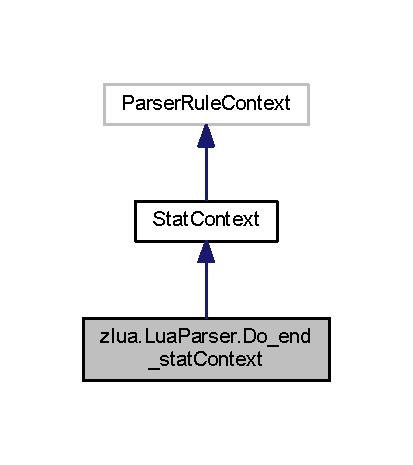
\includegraphics[width=198pt]{classzlua_1_1_lua_parser_1_1_do__end__stat_context__inherit__graph}
\end{center}
\end{figure}


Collaboration diagram for zlua.\+Lua\+Parser.\+Do\+\_\+end\+\_\+stat\+Context\+:
\nopagebreak
\begin{figure}[H]
\begin{center}
\leavevmode
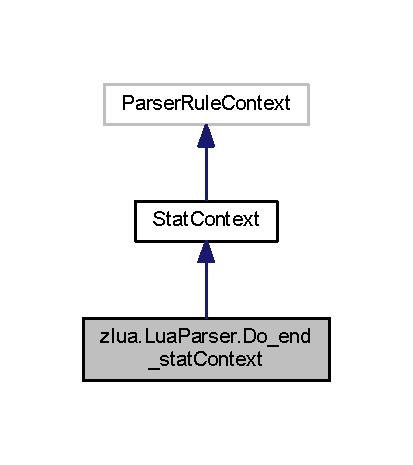
\includegraphics[width=198pt]{classzlua_1_1_lua_parser_1_1_do__end__stat_context__coll__graph}
\end{center}
\end{figure}
\subsection*{Public Member Functions}
\begin{DoxyCompactItemize}
\item 
\mbox{\Hypertarget{classzlua_1_1_lua_parser_1_1_do__end__stat_context_abeca51c056f8e55f868a08b66691c180}\label{classzlua_1_1_lua_parser_1_1_do__end__stat_context_abeca51c056f8e55f868a08b66691c180}} 
\mbox{\hyperlink{classzlua_1_1_lua_parser_1_1_block_context}{Block\+Context}} {\bfseries block} ()
\item 
\mbox{\Hypertarget{classzlua_1_1_lua_parser_1_1_do__end__stat_context_a64dd4479e4b3ac2e1034f3dbefc7e43b}\label{classzlua_1_1_lua_parser_1_1_do__end__stat_context_a64dd4479e4b3ac2e1034f3dbefc7e43b}} 
{\bfseries Do\+\_\+end\+\_\+stat\+Context} (\mbox{\hyperlink{classzlua_1_1_lua_parser_1_1_stat_context}{Stat\+Context}} context)
\item 
\mbox{\Hypertarget{classzlua_1_1_lua_parser_1_1_do__end__stat_context_abc5aef5fc15aab73ddf0438368ba40bc}\label{classzlua_1_1_lua_parser_1_1_do__end__stat_context_abc5aef5fc15aab73ddf0438368ba40bc}} 
override void {\bfseries Enter\+Rule} (I\+Parse\+Tree\+Listener listener)
\item 
\mbox{\Hypertarget{classzlua_1_1_lua_parser_1_1_do__end__stat_context_a7d546013d51aa6e87e30f662765f5975}\label{classzlua_1_1_lua_parser_1_1_do__end__stat_context_a7d546013d51aa6e87e30f662765f5975}} 
override void {\bfseries Exit\+Rule} (I\+Parse\+Tree\+Listener listener)
\item 
\mbox{\Hypertarget{classzlua_1_1_lua_parser_1_1_do__end__stat_context_aece568782ae1d598b98711df82b3117b}\label{classzlua_1_1_lua_parser_1_1_do__end__stat_context_aece568782ae1d598b98711df82b3117b}} 
override T\+Result {\bfseries Accept$<$ T\+Result $>$} (I\+Parse\+Tree\+Visitor$<$ T\+Result $>$ visitor)
\end{DoxyCompactItemize}
\subsection*{Additional Inherited Members}


The documentation for this class was generated from the following file\+:\begin{DoxyCompactItemize}
\item 
zlua/Lua\+Parser.\+cs\end{DoxyCompactItemize}

\hypertarget{classzlua_1_1_lua_parser_1_1_empty__stat_context}{}\section{zlua.\+Lua\+Parser.\+Empty\+\_\+stat\+Context Class Reference}
\label{classzlua_1_1_lua_parser_1_1_empty__stat_context}\index{zlua.\+Lua\+Parser.\+Empty\+\_\+stat\+Context@{zlua.\+Lua\+Parser.\+Empty\+\_\+stat\+Context}}


Inheritance diagram for zlua.\+Lua\+Parser.\+Empty\+\_\+stat\+Context\+:
\nopagebreak
\begin{figure}[H]
\begin{center}
\leavevmode
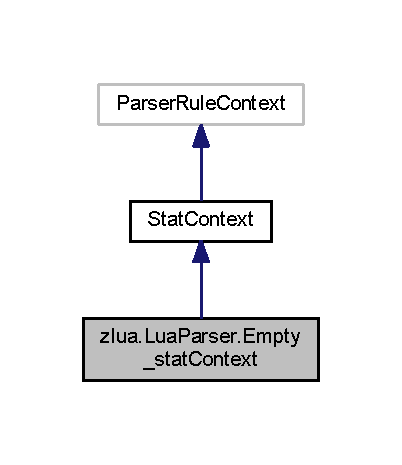
\includegraphics[width=193pt]{classzlua_1_1_lua_parser_1_1_empty__stat_context__inherit__graph}
\end{center}
\end{figure}


Collaboration diagram for zlua.\+Lua\+Parser.\+Empty\+\_\+stat\+Context\+:
\nopagebreak
\begin{figure}[H]
\begin{center}
\leavevmode
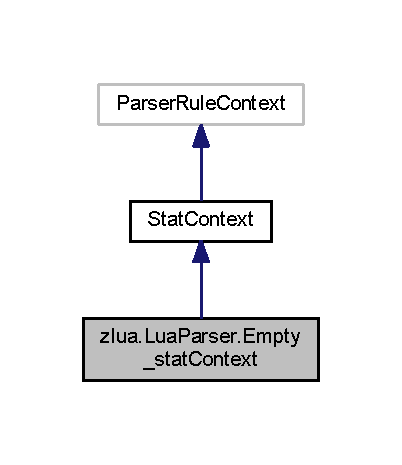
\includegraphics[width=193pt]{classzlua_1_1_lua_parser_1_1_empty__stat_context__coll__graph}
\end{center}
\end{figure}
\subsection*{Public Member Functions}
\begin{DoxyCompactItemize}
\item 
\mbox{\Hypertarget{classzlua_1_1_lua_parser_1_1_empty__stat_context_ad17e975476c62719cea2bdbc23c5994d}\label{classzlua_1_1_lua_parser_1_1_empty__stat_context_ad17e975476c62719cea2bdbc23c5994d}} 
{\bfseries Empty\+\_\+stat\+Context} (\mbox{\hyperlink{classzlua_1_1_lua_parser_1_1_stat_context}{Stat\+Context}} context)
\item 
\mbox{\Hypertarget{classzlua_1_1_lua_parser_1_1_empty__stat_context_aea9a1bf856ba3d7991900f9da48994b0}\label{classzlua_1_1_lua_parser_1_1_empty__stat_context_aea9a1bf856ba3d7991900f9da48994b0}} 
override void {\bfseries Enter\+Rule} (I\+Parse\+Tree\+Listener listener)
\item 
\mbox{\Hypertarget{classzlua_1_1_lua_parser_1_1_empty__stat_context_a07d23cc88827bd396adadf3a0ffe9bf4}\label{classzlua_1_1_lua_parser_1_1_empty__stat_context_a07d23cc88827bd396adadf3a0ffe9bf4}} 
override void {\bfseries Exit\+Rule} (I\+Parse\+Tree\+Listener listener)
\item 
\mbox{\Hypertarget{classzlua_1_1_lua_parser_1_1_empty__stat_context_aa489c47c104dc46439209050bbfc1b7f}\label{classzlua_1_1_lua_parser_1_1_empty__stat_context_aa489c47c104dc46439209050bbfc1b7f}} 
override T\+Result {\bfseries Accept$<$ T\+Result $>$} (I\+Parse\+Tree\+Visitor$<$ T\+Result $>$ visitor)
\end{DoxyCompactItemize}
\subsection*{Additional Inherited Members}


The documentation for this class was generated from the following file\+:\begin{DoxyCompactItemize}
\item 
zlua/Lua\+Parser.\+cs\end{DoxyCompactItemize}

\hypertarget{classzlua_1_1_lua_parser_1_1_exp_context}{}\section{zlua.\+Lua\+Parser.\+Exp\+Context Class Reference}
\label{classzlua_1_1_lua_parser_1_1_exp_context}\index{zlua.\+Lua\+Parser.\+Exp\+Context@{zlua.\+Lua\+Parser.\+Exp\+Context}}


Inheritance diagram for zlua.\+Lua\+Parser.\+Exp\+Context\+:
\nopagebreak
\begin{figure}[H]
\begin{center}
\leavevmode
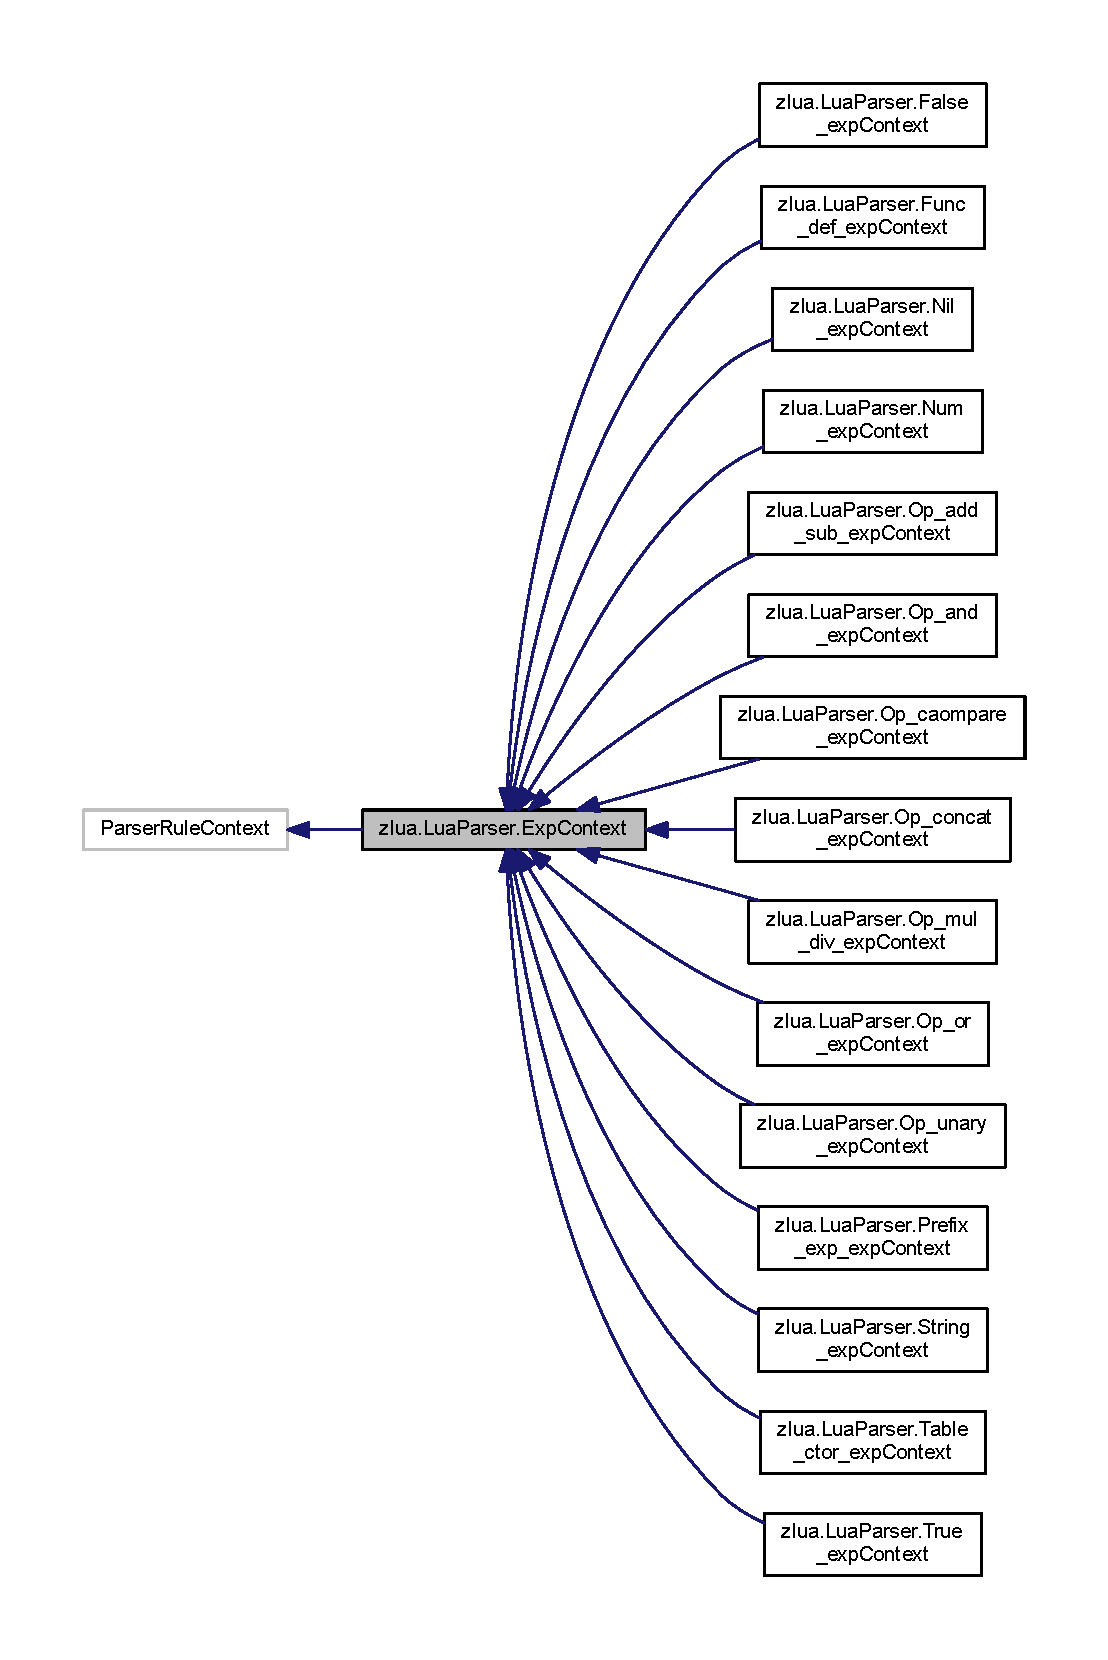
\includegraphics[width=350pt]{classzlua_1_1_lua_parser_1_1_exp_context__inherit__graph}
\end{center}
\end{figure}


Collaboration diagram for zlua.\+Lua\+Parser.\+Exp\+Context\+:
\nopagebreak
\begin{figure}[H]
\begin{center}
\leavevmode
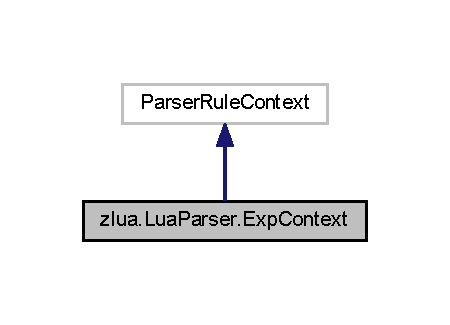
\includegraphics[width=216pt]{classzlua_1_1_lua_parser_1_1_exp_context__coll__graph}
\end{center}
\end{figure}
\subsection*{Public Member Functions}
\begin{DoxyCompactItemize}
\item 
\mbox{\Hypertarget{classzlua_1_1_lua_parser_1_1_exp_context_a896315e970d6e777701e83adc43e1dfd}\label{classzlua_1_1_lua_parser_1_1_exp_context_a896315e970d6e777701e83adc43e1dfd}} 
{\bfseries Exp\+Context} (Parser\+Rule\+Context parent, int invoking\+State)
\item 
\mbox{\Hypertarget{classzlua_1_1_lua_parser_1_1_exp_context_a45a67b74d10763844e6b16b5e1bd480f}\label{classzlua_1_1_lua_parser_1_1_exp_context_a45a67b74d10763844e6b16b5e1bd480f}} 
virtual void {\bfseries Copy\+From} (\mbox{\hyperlink{classzlua_1_1_lua_parser_1_1_exp_context}{Exp\+Context}} context)
\end{DoxyCompactItemize}
\subsection*{Properties}
\begin{DoxyCompactItemize}
\item 
\mbox{\Hypertarget{classzlua_1_1_lua_parser_1_1_exp_context_a3904b8d26d55af399a665555a6451152}\label{classzlua_1_1_lua_parser_1_1_exp_context_a3904b8d26d55af399a665555a6451152}} 
override int {\bfseries Rule\+Index}\hspace{0.3cm}{\ttfamily  \mbox{[}get\mbox{]}}
\end{DoxyCompactItemize}


The documentation for this class was generated from the following file\+:\begin{DoxyCompactItemize}
\item 
zlua/Lua\+Parser.\+cs\end{DoxyCompactItemize}

\hypertarget{classzlua_1_1_lua_parser_1_1_explist_context}{}\section{zlua.\+Lua\+Parser.\+Explist\+Context Class Reference}
\label{classzlua_1_1_lua_parser_1_1_explist_context}\index{zlua.\+Lua\+Parser.\+Explist\+Context@{zlua.\+Lua\+Parser.\+Explist\+Context}}


Inheritance diagram for zlua.\+Lua\+Parser.\+Explist\+Context\+:
\nopagebreak
\begin{figure}[H]
\begin{center}
\leavevmode
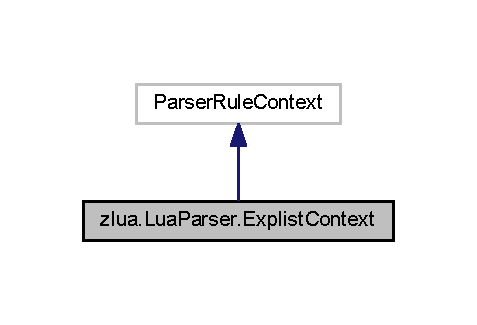
\includegraphics[width=229pt]{classzlua_1_1_lua_parser_1_1_explist_context__inherit__graph}
\end{center}
\end{figure}


Collaboration diagram for zlua.\+Lua\+Parser.\+Explist\+Context\+:
\nopagebreak
\begin{figure}[H]
\begin{center}
\leavevmode
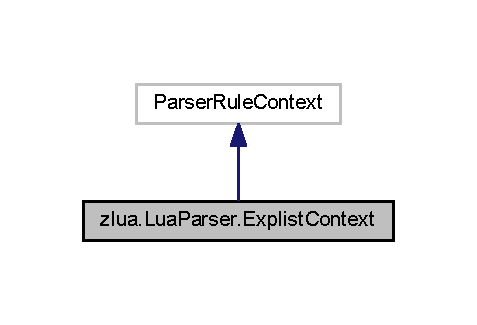
\includegraphics[width=229pt]{classzlua_1_1_lua_parser_1_1_explist_context__coll__graph}
\end{center}
\end{figure}
\subsection*{Public Member Functions}
\begin{DoxyCompactItemize}
\item 
\mbox{\Hypertarget{classzlua_1_1_lua_parser_1_1_explist_context_aa0b980d461da890c56a59f8cbacd1052}\label{classzlua_1_1_lua_parser_1_1_explist_context_aa0b980d461da890c56a59f8cbacd1052}} 
\mbox{\hyperlink{classzlua_1_1_lua_parser_1_1_exp_context}{Exp\+Context}} \mbox{[}$\,$\mbox{]} {\bfseries exp} ()
\item 
\mbox{\Hypertarget{classzlua_1_1_lua_parser_1_1_explist_context_a461f6d5e3b103152e90ec4c59ea163dd}\label{classzlua_1_1_lua_parser_1_1_explist_context_a461f6d5e3b103152e90ec4c59ea163dd}} 
\mbox{\hyperlink{classzlua_1_1_lua_parser_1_1_exp_context}{Exp\+Context}} {\bfseries exp} (int i)
\item 
\mbox{\Hypertarget{classzlua_1_1_lua_parser_1_1_explist_context_a2b4a17f2475dafff00945c68272e3ea4}\label{classzlua_1_1_lua_parser_1_1_explist_context_a2b4a17f2475dafff00945c68272e3ea4}} 
{\bfseries Explist\+Context} (Parser\+Rule\+Context parent, int invoking\+State)
\item 
\mbox{\Hypertarget{classzlua_1_1_lua_parser_1_1_explist_context_a1a8806cd4e6691952eb5542f51e5c854}\label{classzlua_1_1_lua_parser_1_1_explist_context_a1a8806cd4e6691952eb5542f51e5c854}} 
override void {\bfseries Enter\+Rule} (I\+Parse\+Tree\+Listener listener)
\item 
\mbox{\Hypertarget{classzlua_1_1_lua_parser_1_1_explist_context_a9461c28bf898cc673cebeff271315b2b}\label{classzlua_1_1_lua_parser_1_1_explist_context_a9461c28bf898cc673cebeff271315b2b}} 
override void {\bfseries Exit\+Rule} (I\+Parse\+Tree\+Listener listener)
\item 
\mbox{\Hypertarget{classzlua_1_1_lua_parser_1_1_explist_context_a149432b9718df4e6b3617aa530f54e77}\label{classzlua_1_1_lua_parser_1_1_explist_context_a149432b9718df4e6b3617aa530f54e77}} 
override T\+Result {\bfseries Accept$<$ T\+Result $>$} (I\+Parse\+Tree\+Visitor$<$ T\+Result $>$ visitor)
\end{DoxyCompactItemize}
\subsection*{Properties}
\begin{DoxyCompactItemize}
\item 
\mbox{\Hypertarget{classzlua_1_1_lua_parser_1_1_explist_context_ad0cb06f2973e4aad5bf47b67723fe347}\label{classzlua_1_1_lua_parser_1_1_explist_context_ad0cb06f2973e4aad5bf47b67723fe347}} 
override int {\bfseries Rule\+Index}\hspace{0.3cm}{\ttfamily  \mbox{[}get\mbox{]}}
\end{DoxyCompactItemize}


The documentation for this class was generated from the following file\+:\begin{DoxyCompactItemize}
\item 
zlua/Lua\+Parser.\+cs\end{DoxyCompactItemize}

\hypertarget{classzlua_1_1_lua_parser_1_1_false__exp_context}{}\section{zlua.\+Lua\+Parser.\+False\+\_\+exp\+Context Class Reference}
\label{classzlua_1_1_lua_parser_1_1_false__exp_context}\index{zlua.\+Lua\+Parser.\+False\+\_\+exp\+Context@{zlua.\+Lua\+Parser.\+False\+\_\+exp\+Context}}


Inheritance diagram for zlua.\+Lua\+Parser.\+False\+\_\+exp\+Context\+:
\nopagebreak
\begin{figure}[H]
\begin{center}
\leavevmode
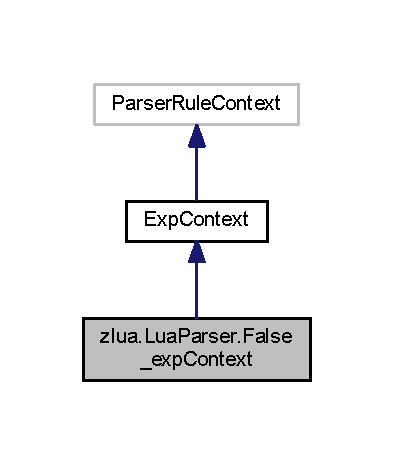
\includegraphics[width=189pt]{classzlua_1_1_lua_parser_1_1_false__exp_context__inherit__graph}
\end{center}
\end{figure}


Collaboration diagram for zlua.\+Lua\+Parser.\+False\+\_\+exp\+Context\+:
\nopagebreak
\begin{figure}[H]
\begin{center}
\leavevmode
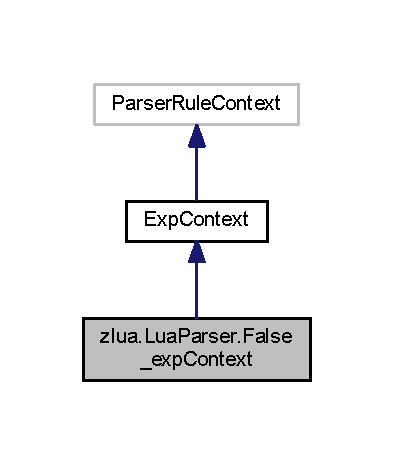
\includegraphics[width=189pt]{classzlua_1_1_lua_parser_1_1_false__exp_context__coll__graph}
\end{center}
\end{figure}
\subsection*{Public Member Functions}
\begin{DoxyCompactItemize}
\item 
\mbox{\Hypertarget{classzlua_1_1_lua_parser_1_1_false__exp_context_a066129971f105fe49aa323a2e0ed29c5}\label{classzlua_1_1_lua_parser_1_1_false__exp_context_a066129971f105fe49aa323a2e0ed29c5}} 
{\bfseries False\+\_\+exp\+Context} (\mbox{\hyperlink{classzlua_1_1_lua_parser_1_1_exp_context}{Exp\+Context}} context)
\item 
\mbox{\Hypertarget{classzlua_1_1_lua_parser_1_1_false__exp_context_ae0f16242c9c8b34a0d7a8915640aa41b}\label{classzlua_1_1_lua_parser_1_1_false__exp_context_ae0f16242c9c8b34a0d7a8915640aa41b}} 
override void {\bfseries Enter\+Rule} (I\+Parse\+Tree\+Listener listener)
\item 
\mbox{\Hypertarget{classzlua_1_1_lua_parser_1_1_false__exp_context_aa3b1aaf503e07aabfa3c085f70139c86}\label{classzlua_1_1_lua_parser_1_1_false__exp_context_aa3b1aaf503e07aabfa3c085f70139c86}} 
override void {\bfseries Exit\+Rule} (I\+Parse\+Tree\+Listener listener)
\item 
\mbox{\Hypertarget{classzlua_1_1_lua_parser_1_1_false__exp_context_a0aac6f1b4b3e4c95f944bb1162166320}\label{classzlua_1_1_lua_parser_1_1_false__exp_context_a0aac6f1b4b3e4c95f944bb1162166320}} 
override T\+Result {\bfseries Accept$<$ T\+Result $>$} (I\+Parse\+Tree\+Visitor$<$ T\+Result $>$ visitor)
\end{DoxyCompactItemize}
\subsection*{Additional Inherited Members}


The documentation for this class was generated from the following file\+:\begin{DoxyCompactItemize}
\item 
zlua/Lua\+Parser.\+cs\end{DoxyCompactItemize}

\hypertarget{classzlua_1_1_lua_parser_1_1_field_context}{}\section{zlua.\+Lua\+Parser.\+Field\+Context Class Reference}
\label{classzlua_1_1_lua_parser_1_1_field_context}\index{zlua.\+Lua\+Parser.\+Field\+Context@{zlua.\+Lua\+Parser.\+Field\+Context}}


Inheritance diagram for zlua.\+Lua\+Parser.\+Field\+Context\+:
\nopagebreak
\begin{figure}[H]
\begin{center}
\leavevmode
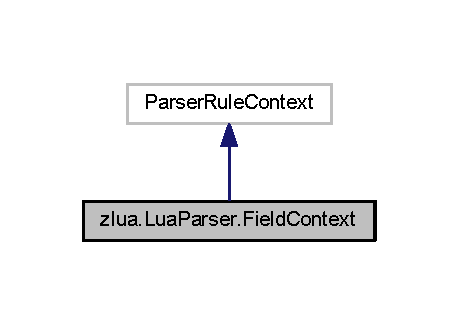
\includegraphics[width=220pt]{classzlua_1_1_lua_parser_1_1_field_context__inherit__graph}
\end{center}
\end{figure}


Collaboration diagram for zlua.\+Lua\+Parser.\+Field\+Context\+:
\nopagebreak
\begin{figure}[H]
\begin{center}
\leavevmode
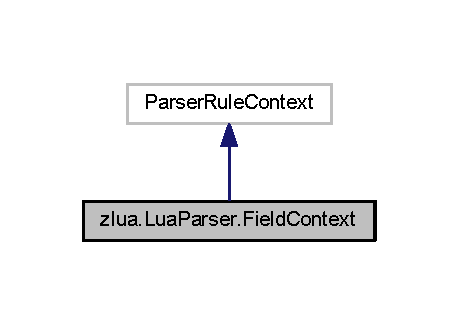
\includegraphics[width=220pt]{classzlua_1_1_lua_parser_1_1_field_context__coll__graph}
\end{center}
\end{figure}
\subsection*{Public Member Functions}
\begin{DoxyCompactItemize}
\item 
\mbox{\Hypertarget{classzlua_1_1_lua_parser_1_1_field_context_af0f3069d6a75841c84261ac120d11c1e}\label{classzlua_1_1_lua_parser_1_1_field_context_af0f3069d6a75841c84261ac120d11c1e}} 
\mbox{\hyperlink{classzlua_1_1_lua_parser_1_1_exp_context}{Exp\+Context}} \mbox{[}$\,$\mbox{]} {\bfseries exp} ()
\item 
\mbox{\Hypertarget{classzlua_1_1_lua_parser_1_1_field_context_ab46b73d545118459c7de9104d7088433}\label{classzlua_1_1_lua_parser_1_1_field_context_ab46b73d545118459c7de9104d7088433}} 
\mbox{\hyperlink{classzlua_1_1_lua_parser_1_1_exp_context}{Exp\+Context}} {\bfseries exp} (int i)
\item 
\mbox{\Hypertarget{classzlua_1_1_lua_parser_1_1_field_context_a95d8cdae083920fa6a668a5c18ebdbc9}\label{classzlua_1_1_lua_parser_1_1_field_context_a95d8cdae083920fa6a668a5c18ebdbc9}} 
I\+Terminal\+Node {\bfseries N\+A\+ME} ()
\item 
\mbox{\Hypertarget{classzlua_1_1_lua_parser_1_1_field_context_afedb127158a075e7dbe2f35706c7bbed}\label{classzlua_1_1_lua_parser_1_1_field_context_afedb127158a075e7dbe2f35706c7bbed}} 
{\bfseries Field\+Context} (Parser\+Rule\+Context parent, int invoking\+State)
\item 
\mbox{\Hypertarget{classzlua_1_1_lua_parser_1_1_field_context_ad61a7f19c4830c34478bc73e91f187e3}\label{classzlua_1_1_lua_parser_1_1_field_context_ad61a7f19c4830c34478bc73e91f187e3}} 
override void {\bfseries Enter\+Rule} (I\+Parse\+Tree\+Listener listener)
\item 
\mbox{\Hypertarget{classzlua_1_1_lua_parser_1_1_field_context_a4876ac018d9668a7cb374c6095c8622b}\label{classzlua_1_1_lua_parser_1_1_field_context_a4876ac018d9668a7cb374c6095c8622b}} 
override void {\bfseries Exit\+Rule} (I\+Parse\+Tree\+Listener listener)
\item 
\mbox{\Hypertarget{classzlua_1_1_lua_parser_1_1_field_context_ab07e61d8a13d29243cfa63ffd6e3218c}\label{classzlua_1_1_lua_parser_1_1_field_context_ab07e61d8a13d29243cfa63ffd6e3218c}} 
override T\+Result {\bfseries Accept$<$ T\+Result $>$} (I\+Parse\+Tree\+Visitor$<$ T\+Result $>$ visitor)
\end{DoxyCompactItemize}
\subsection*{Properties}
\begin{DoxyCompactItemize}
\item 
\mbox{\Hypertarget{classzlua_1_1_lua_parser_1_1_field_context_a295ae239b384e10ed543b537eabc4034}\label{classzlua_1_1_lua_parser_1_1_field_context_a295ae239b384e10ed543b537eabc4034}} 
override int {\bfseries Rule\+Index}\hspace{0.3cm}{\ttfamily  \mbox{[}get\mbox{]}}
\end{DoxyCompactItemize}


The documentation for this class was generated from the following file\+:\begin{DoxyCompactItemize}
\item 
zlua/Lua\+Parser.\+cs\end{DoxyCompactItemize}

\hypertarget{classzlua_1_1_lua_parser_1_1_fieldlist_context}{}\section{zlua.\+Lua\+Parser.\+Fieldlist\+Context Class Reference}
\label{classzlua_1_1_lua_parser_1_1_fieldlist_context}\index{zlua.\+Lua\+Parser.\+Fieldlist\+Context@{zlua.\+Lua\+Parser.\+Fieldlist\+Context}}


Inheritance diagram for zlua.\+Lua\+Parser.\+Fieldlist\+Context\+:
\nopagebreak
\begin{figure}[H]
\begin{center}
\leavevmode
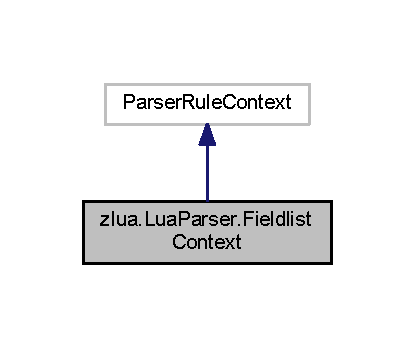
\includegraphics[width=199pt]{classzlua_1_1_lua_parser_1_1_fieldlist_context__inherit__graph}
\end{center}
\end{figure}


Collaboration diagram for zlua.\+Lua\+Parser.\+Fieldlist\+Context\+:
\nopagebreak
\begin{figure}[H]
\begin{center}
\leavevmode
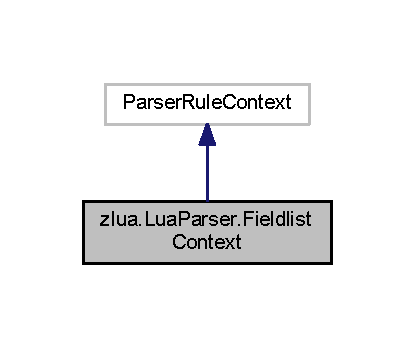
\includegraphics[width=199pt]{classzlua_1_1_lua_parser_1_1_fieldlist_context__coll__graph}
\end{center}
\end{figure}
\subsection*{Public Member Functions}
\begin{DoxyCompactItemize}
\item 
\mbox{\Hypertarget{classzlua_1_1_lua_parser_1_1_fieldlist_context_af23c267c9d523ddb307a9b2212182e56}\label{classzlua_1_1_lua_parser_1_1_fieldlist_context_af23c267c9d523ddb307a9b2212182e56}} 
\mbox{\hyperlink{classzlua_1_1_lua_parser_1_1_field_context}{Field\+Context}} \mbox{[}$\,$\mbox{]} {\bfseries field} ()
\item 
\mbox{\Hypertarget{classzlua_1_1_lua_parser_1_1_fieldlist_context_a04808cb40c2c64b0728b69e814961cfa}\label{classzlua_1_1_lua_parser_1_1_fieldlist_context_a04808cb40c2c64b0728b69e814961cfa}} 
\mbox{\hyperlink{classzlua_1_1_lua_parser_1_1_field_context}{Field\+Context}} {\bfseries field} (int i)
\item 
\mbox{\Hypertarget{classzlua_1_1_lua_parser_1_1_fieldlist_context_a8424fe4821feb1d99c5dc6d167aa33e4}\label{classzlua_1_1_lua_parser_1_1_fieldlist_context_a8424fe4821feb1d99c5dc6d167aa33e4}} 
\mbox{\hyperlink{classzlua_1_1_lua_parser_1_1_fieldsep_context}{Fieldsep\+Context}} \mbox{[}$\,$\mbox{]} {\bfseries fieldsep} ()
\item 
\mbox{\Hypertarget{classzlua_1_1_lua_parser_1_1_fieldlist_context_ad782722b3bc7ee0cd36731dc721ca848}\label{classzlua_1_1_lua_parser_1_1_fieldlist_context_ad782722b3bc7ee0cd36731dc721ca848}} 
\mbox{\hyperlink{classzlua_1_1_lua_parser_1_1_fieldsep_context}{Fieldsep\+Context}} {\bfseries fieldsep} (int i)
\item 
\mbox{\Hypertarget{classzlua_1_1_lua_parser_1_1_fieldlist_context_ada3b3444401a79a3e0d15594ad690fae}\label{classzlua_1_1_lua_parser_1_1_fieldlist_context_ada3b3444401a79a3e0d15594ad690fae}} 
{\bfseries Fieldlist\+Context} (Parser\+Rule\+Context parent, int invoking\+State)
\item 
\mbox{\Hypertarget{classzlua_1_1_lua_parser_1_1_fieldlist_context_a4a967e8f50aabec16080e5525976d9ee}\label{classzlua_1_1_lua_parser_1_1_fieldlist_context_a4a967e8f50aabec16080e5525976d9ee}} 
override void {\bfseries Enter\+Rule} (I\+Parse\+Tree\+Listener listener)
\item 
\mbox{\Hypertarget{classzlua_1_1_lua_parser_1_1_fieldlist_context_a023b3d1aebdbb731ec0c8d841f39b00b}\label{classzlua_1_1_lua_parser_1_1_fieldlist_context_a023b3d1aebdbb731ec0c8d841f39b00b}} 
override void {\bfseries Exit\+Rule} (I\+Parse\+Tree\+Listener listener)
\item 
\mbox{\Hypertarget{classzlua_1_1_lua_parser_1_1_fieldlist_context_ad7bf67fc8cfa0133e99bddbc1a875c89}\label{classzlua_1_1_lua_parser_1_1_fieldlist_context_ad7bf67fc8cfa0133e99bddbc1a875c89}} 
override T\+Result {\bfseries Accept$<$ T\+Result $>$} (I\+Parse\+Tree\+Visitor$<$ T\+Result $>$ visitor)
\end{DoxyCompactItemize}
\subsection*{Properties}
\begin{DoxyCompactItemize}
\item 
\mbox{\Hypertarget{classzlua_1_1_lua_parser_1_1_fieldlist_context_aeb724ccb91fcd2f01ab587dfcf608b7f}\label{classzlua_1_1_lua_parser_1_1_fieldlist_context_aeb724ccb91fcd2f01ab587dfcf608b7f}} 
override int {\bfseries Rule\+Index}\hspace{0.3cm}{\ttfamily  \mbox{[}get\mbox{]}}
\end{DoxyCompactItemize}


The documentation for this class was generated from the following file\+:\begin{DoxyCompactItemize}
\item 
zlua/Lua\+Parser.\+cs\end{DoxyCompactItemize}

\hypertarget{classzlua_1_1_lua_parser_1_1_fieldsep_context}{}\section{zlua.\+Lua\+Parser.\+Fieldsep\+Context Class Reference}
\label{classzlua_1_1_lua_parser_1_1_fieldsep_context}\index{zlua.\+Lua\+Parser.\+Fieldsep\+Context@{zlua.\+Lua\+Parser.\+Fieldsep\+Context}}


Inheritance diagram for zlua.\+Lua\+Parser.\+Fieldsep\+Context\+:
\nopagebreak
\begin{figure}[H]
\begin{center}
\leavevmode
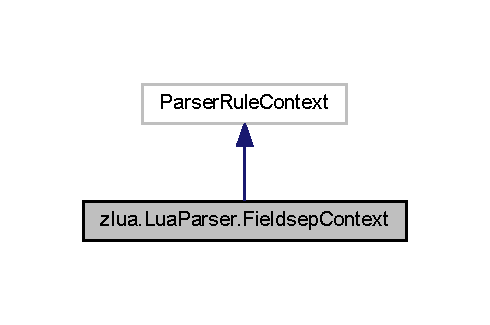
\includegraphics[width=235pt]{classzlua_1_1_lua_parser_1_1_fieldsep_context__inherit__graph}
\end{center}
\end{figure}


Collaboration diagram for zlua.\+Lua\+Parser.\+Fieldsep\+Context\+:
\nopagebreak
\begin{figure}[H]
\begin{center}
\leavevmode
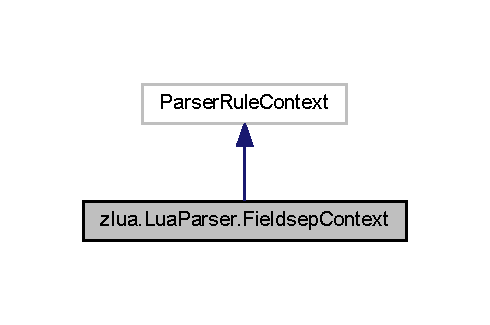
\includegraphics[width=235pt]{classzlua_1_1_lua_parser_1_1_fieldsep_context__coll__graph}
\end{center}
\end{figure}
\subsection*{Public Member Functions}
\begin{DoxyCompactItemize}
\item 
\mbox{\Hypertarget{classzlua_1_1_lua_parser_1_1_fieldsep_context_a4bce479ab9aa0661b63e47a29b949c62}\label{classzlua_1_1_lua_parser_1_1_fieldsep_context_a4bce479ab9aa0661b63e47a29b949c62}} 
{\bfseries Fieldsep\+Context} (Parser\+Rule\+Context parent, int invoking\+State)
\item 
\mbox{\Hypertarget{classzlua_1_1_lua_parser_1_1_fieldsep_context_ae5aa1cff79f8a3d90edd6d4214ae829c}\label{classzlua_1_1_lua_parser_1_1_fieldsep_context_ae5aa1cff79f8a3d90edd6d4214ae829c}} 
override void {\bfseries Enter\+Rule} (I\+Parse\+Tree\+Listener listener)
\item 
\mbox{\Hypertarget{classzlua_1_1_lua_parser_1_1_fieldsep_context_a80a317c7aa832212d78d97444bb1c919}\label{classzlua_1_1_lua_parser_1_1_fieldsep_context_a80a317c7aa832212d78d97444bb1c919}} 
override void {\bfseries Exit\+Rule} (I\+Parse\+Tree\+Listener listener)
\item 
\mbox{\Hypertarget{classzlua_1_1_lua_parser_1_1_fieldsep_context_a6518594361fcbfcb276ff7164105634b}\label{classzlua_1_1_lua_parser_1_1_fieldsep_context_a6518594361fcbfcb276ff7164105634b}} 
override T\+Result {\bfseries Accept$<$ T\+Result $>$} (I\+Parse\+Tree\+Visitor$<$ T\+Result $>$ visitor)
\end{DoxyCompactItemize}
\subsection*{Properties}
\begin{DoxyCompactItemize}
\item 
\mbox{\Hypertarget{classzlua_1_1_lua_parser_1_1_fieldsep_context_a2590c6671398bf7c0e0fd0e16c4c5b40}\label{classzlua_1_1_lua_parser_1_1_fieldsep_context_a2590c6671398bf7c0e0fd0e16c4c5b40}} 
override int {\bfseries Rule\+Index}\hspace{0.3cm}{\ttfamily  \mbox{[}get\mbox{]}}
\end{DoxyCompactItemize}


The documentation for this class was generated from the following file\+:\begin{DoxyCompactItemize}
\item 
zlua/Lua\+Parser.\+cs\end{DoxyCompactItemize}

\hypertarget{classzlua_1_1_lua_parser_1_1_func__call__stat_context}{}\section{zlua.\+Lua\+Parser.\+Func\+\_\+call\+\_\+stat\+Context Class Reference}
\label{classzlua_1_1_lua_parser_1_1_func__call__stat_context}\index{zlua.\+Lua\+Parser.\+Func\+\_\+call\+\_\+stat\+Context@{zlua.\+Lua\+Parser.\+Func\+\_\+call\+\_\+stat\+Context}}


Inheritance diagram for zlua.\+Lua\+Parser.\+Func\+\_\+call\+\_\+stat\+Context\+:
\nopagebreak
\begin{figure}[H]
\begin{center}
\leavevmode
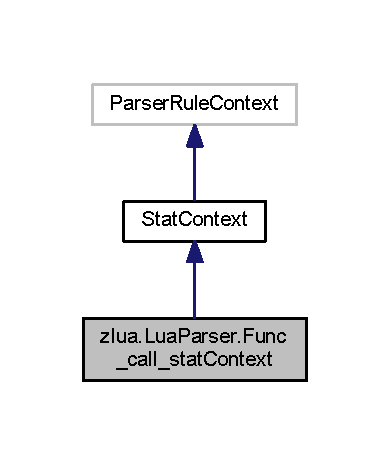
\includegraphics[width=187pt]{classzlua_1_1_lua_parser_1_1_func__call__stat_context__inherit__graph}
\end{center}
\end{figure}


Collaboration diagram for zlua.\+Lua\+Parser.\+Func\+\_\+call\+\_\+stat\+Context\+:
\nopagebreak
\begin{figure}[H]
\begin{center}
\leavevmode
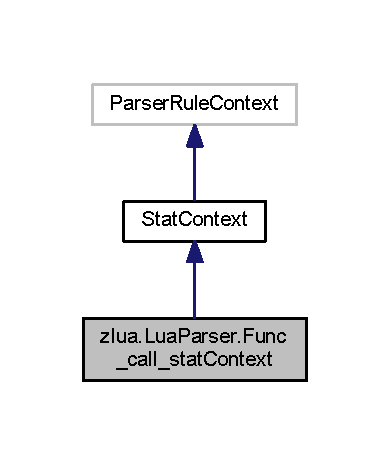
\includegraphics[width=187pt]{classzlua_1_1_lua_parser_1_1_func__call__stat_context__coll__graph}
\end{center}
\end{figure}
\subsection*{Public Member Functions}
\begin{DoxyCompactItemize}
\item 
\mbox{\Hypertarget{classzlua_1_1_lua_parser_1_1_func__call__stat_context_a32d3406f052ead20bc61b1ddc3087dad}\label{classzlua_1_1_lua_parser_1_1_func__call__stat_context_a32d3406f052ead20bc61b1ddc3087dad}} 
\mbox{\hyperlink{classzlua_1_1_lua_parser_1_1_functioncall_context}{Functioncall\+Context}} {\bfseries functioncall} ()
\item 
\mbox{\Hypertarget{classzlua_1_1_lua_parser_1_1_func__call__stat_context_ad6f542ac2da7617814d55c090bfbfa4b}\label{classzlua_1_1_lua_parser_1_1_func__call__stat_context_ad6f542ac2da7617814d55c090bfbfa4b}} 
{\bfseries Func\+\_\+call\+\_\+stat\+Context} (\mbox{\hyperlink{classzlua_1_1_lua_parser_1_1_stat_context}{Stat\+Context}} context)
\item 
\mbox{\Hypertarget{classzlua_1_1_lua_parser_1_1_func__call__stat_context_a2684f23aa335f0310ccc266c82329535}\label{classzlua_1_1_lua_parser_1_1_func__call__stat_context_a2684f23aa335f0310ccc266c82329535}} 
override void {\bfseries Enter\+Rule} (I\+Parse\+Tree\+Listener listener)
\item 
\mbox{\Hypertarget{classzlua_1_1_lua_parser_1_1_func__call__stat_context_af5f3da5db84f471215668f79c226d55b}\label{classzlua_1_1_lua_parser_1_1_func__call__stat_context_af5f3da5db84f471215668f79c226d55b}} 
override void {\bfseries Exit\+Rule} (I\+Parse\+Tree\+Listener listener)
\item 
\mbox{\Hypertarget{classzlua_1_1_lua_parser_1_1_func__call__stat_context_ad88cbcc31be648c2c3cf3e19c6518609}\label{classzlua_1_1_lua_parser_1_1_func__call__stat_context_ad88cbcc31be648c2c3cf3e19c6518609}} 
override T\+Result {\bfseries Accept$<$ T\+Result $>$} (I\+Parse\+Tree\+Visitor$<$ T\+Result $>$ visitor)
\end{DoxyCompactItemize}
\subsection*{Additional Inherited Members}


The documentation for this class was generated from the following file\+:\begin{DoxyCompactItemize}
\item 
zlua/Lua\+Parser.\+cs\end{DoxyCompactItemize}

\hypertarget{classzlua_1_1_lua_parser_1_1_func__def__exp_context}{}\section{zlua.\+Lua\+Parser.\+Func\+\_\+def\+\_\+exp\+Context Class Reference}
\label{classzlua_1_1_lua_parser_1_1_func__def__exp_context}\index{zlua.\+Lua\+Parser.\+Func\+\_\+def\+\_\+exp\+Context@{zlua.\+Lua\+Parser.\+Func\+\_\+def\+\_\+exp\+Context}}


Inheritance diagram for zlua.\+Lua\+Parser.\+Func\+\_\+def\+\_\+exp\+Context\+:
\nopagebreak
\begin{figure}[H]
\begin{center}
\leavevmode
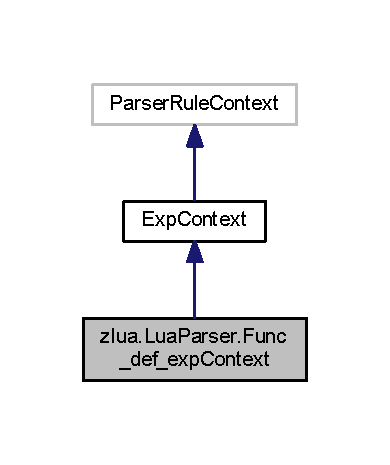
\includegraphics[width=187pt]{classzlua_1_1_lua_parser_1_1_func__def__exp_context__inherit__graph}
\end{center}
\end{figure}


Collaboration diagram for zlua.\+Lua\+Parser.\+Func\+\_\+def\+\_\+exp\+Context\+:
\nopagebreak
\begin{figure}[H]
\begin{center}
\leavevmode
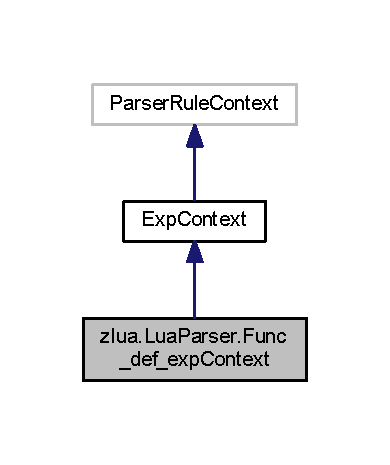
\includegraphics[width=187pt]{classzlua_1_1_lua_parser_1_1_func__def__exp_context__coll__graph}
\end{center}
\end{figure}
\subsection*{Public Member Functions}
\begin{DoxyCompactItemize}
\item 
\mbox{\Hypertarget{classzlua_1_1_lua_parser_1_1_func__def__exp_context_adadd5ba1a20549a108d48fd3d516536c}\label{classzlua_1_1_lua_parser_1_1_func__def__exp_context_adadd5ba1a20549a108d48fd3d516536c}} 
\mbox{\hyperlink{classzlua_1_1_lua_parser_1_1_functiondef_context}{Functiondef\+Context}} {\bfseries functiondef} ()
\item 
\mbox{\Hypertarget{classzlua_1_1_lua_parser_1_1_func__def__exp_context_a67a74ed05a671b40140778edf374924c}\label{classzlua_1_1_lua_parser_1_1_func__def__exp_context_a67a74ed05a671b40140778edf374924c}} 
{\bfseries Func\+\_\+def\+\_\+exp\+Context} (\mbox{\hyperlink{classzlua_1_1_lua_parser_1_1_exp_context}{Exp\+Context}} context)
\item 
\mbox{\Hypertarget{classzlua_1_1_lua_parser_1_1_func__def__exp_context_afe2f0df88bf37876585fdae3c8c1a7a8}\label{classzlua_1_1_lua_parser_1_1_func__def__exp_context_afe2f0df88bf37876585fdae3c8c1a7a8}} 
override void {\bfseries Enter\+Rule} (I\+Parse\+Tree\+Listener listener)
\item 
\mbox{\Hypertarget{classzlua_1_1_lua_parser_1_1_func__def__exp_context_ac83d270e2398b8dbaf4745d9fed5b9b0}\label{classzlua_1_1_lua_parser_1_1_func__def__exp_context_ac83d270e2398b8dbaf4745d9fed5b9b0}} 
override void {\bfseries Exit\+Rule} (I\+Parse\+Tree\+Listener listener)
\item 
\mbox{\Hypertarget{classzlua_1_1_lua_parser_1_1_func__def__exp_context_a19b4cf0237afb89de8f09e50c132dfa5}\label{classzlua_1_1_lua_parser_1_1_func__def__exp_context_a19b4cf0237afb89de8f09e50c132dfa5}} 
override T\+Result {\bfseries Accept$<$ T\+Result $>$} (I\+Parse\+Tree\+Visitor$<$ T\+Result $>$ visitor)
\end{DoxyCompactItemize}
\subsection*{Additional Inherited Members}


The documentation for this class was generated from the following file\+:\begin{DoxyCompactItemize}
\item 
zlua/Lua\+Parser.\+cs\end{DoxyCompactItemize}

\hypertarget{classzlua_1_1_lua_parser_1_1_func__def__stat_context}{}\section{zlua.\+Lua\+Parser.\+Func\+\_\+def\+\_\+stat\+Context Class Reference}
\label{classzlua_1_1_lua_parser_1_1_func__def__stat_context}\index{zlua.\+Lua\+Parser.\+Func\+\_\+def\+\_\+stat\+Context@{zlua.\+Lua\+Parser.\+Func\+\_\+def\+\_\+stat\+Context}}


Inheritance diagram for zlua.\+Lua\+Parser.\+Func\+\_\+def\+\_\+stat\+Context\+:
\nopagebreak
\begin{figure}[H]
\begin{center}
\leavevmode
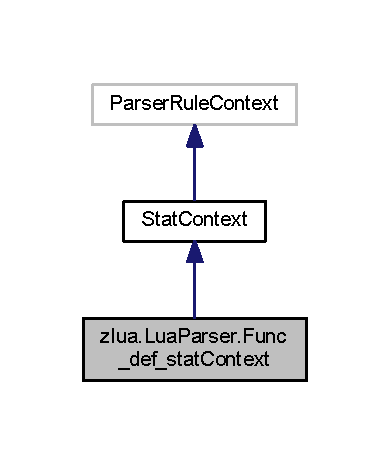
\includegraphics[width=187pt]{classzlua_1_1_lua_parser_1_1_func__def__stat_context__inherit__graph}
\end{center}
\end{figure}


Collaboration diagram for zlua.\+Lua\+Parser.\+Func\+\_\+def\+\_\+stat\+Context\+:
\nopagebreak
\begin{figure}[H]
\begin{center}
\leavevmode
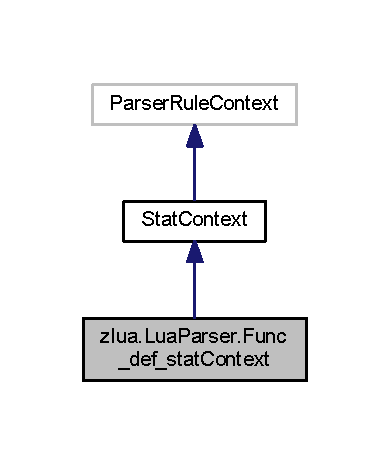
\includegraphics[width=187pt]{classzlua_1_1_lua_parser_1_1_func__def__stat_context__coll__graph}
\end{center}
\end{figure}
\subsection*{Public Member Functions}
\begin{DoxyCompactItemize}
\item 
\mbox{\Hypertarget{classzlua_1_1_lua_parser_1_1_func__def__stat_context_aab1ed338258ef2cf357fcfc640b96e9b}\label{classzlua_1_1_lua_parser_1_1_func__def__stat_context_aab1ed338258ef2cf357fcfc640b96e9b}} 
\mbox{\hyperlink{classzlua_1_1_lua_parser_1_1_funcname_context}{Funcname\+Context}} {\bfseries funcname} ()
\item 
\mbox{\Hypertarget{classzlua_1_1_lua_parser_1_1_func__def__stat_context_abd042137a995ad4494e3a70dbb576824}\label{classzlua_1_1_lua_parser_1_1_func__def__stat_context_abd042137a995ad4494e3a70dbb576824}} 
\mbox{\hyperlink{classzlua_1_1_lua_parser_1_1_funcbody_context}{Funcbody\+Context}} {\bfseries funcbody} ()
\item 
\mbox{\Hypertarget{classzlua_1_1_lua_parser_1_1_func__def__stat_context_aa87a50bceee612f9c436091d53954ba6}\label{classzlua_1_1_lua_parser_1_1_func__def__stat_context_aa87a50bceee612f9c436091d53954ba6}} 
{\bfseries Func\+\_\+def\+\_\+stat\+Context} (\mbox{\hyperlink{classzlua_1_1_lua_parser_1_1_stat_context}{Stat\+Context}} context)
\item 
\mbox{\Hypertarget{classzlua_1_1_lua_parser_1_1_func__def__stat_context_ab2af58e0afaa632a3be0a0926f1919cc}\label{classzlua_1_1_lua_parser_1_1_func__def__stat_context_ab2af58e0afaa632a3be0a0926f1919cc}} 
override void {\bfseries Enter\+Rule} (I\+Parse\+Tree\+Listener listener)
\item 
\mbox{\Hypertarget{classzlua_1_1_lua_parser_1_1_func__def__stat_context_a7912184a230d54af743198c02f2df412}\label{classzlua_1_1_lua_parser_1_1_func__def__stat_context_a7912184a230d54af743198c02f2df412}} 
override void {\bfseries Exit\+Rule} (I\+Parse\+Tree\+Listener listener)
\item 
\mbox{\Hypertarget{classzlua_1_1_lua_parser_1_1_func__def__stat_context_a3e651a8a4aa240ec8602388e9af61eff}\label{classzlua_1_1_lua_parser_1_1_func__def__stat_context_a3e651a8a4aa240ec8602388e9af61eff}} 
override T\+Result {\bfseries Accept$<$ T\+Result $>$} (I\+Parse\+Tree\+Visitor$<$ T\+Result $>$ visitor)
\end{DoxyCompactItemize}
\subsection*{Additional Inherited Members}


The documentation for this class was generated from the following file\+:\begin{DoxyCompactItemize}
\item 
zlua/Lua\+Parser.\+cs\end{DoxyCompactItemize}

\hypertarget{classzlua_1_1_lua_parser_1_1_funcbody_context}{}\section{zlua.\+Lua\+Parser.\+Funcbody\+Context Class Reference}
\label{classzlua_1_1_lua_parser_1_1_funcbody_context}\index{zlua.\+Lua\+Parser.\+Funcbody\+Context@{zlua.\+Lua\+Parser.\+Funcbody\+Context}}


Inheritance diagram for zlua.\+Lua\+Parser.\+Funcbody\+Context\+:
\nopagebreak
\begin{figure}[H]
\begin{center}
\leavevmode
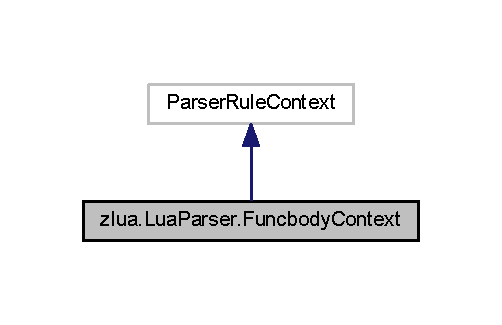
\includegraphics[width=241pt]{classzlua_1_1_lua_parser_1_1_funcbody_context__inherit__graph}
\end{center}
\end{figure}


Collaboration diagram for zlua.\+Lua\+Parser.\+Funcbody\+Context\+:
\nopagebreak
\begin{figure}[H]
\begin{center}
\leavevmode
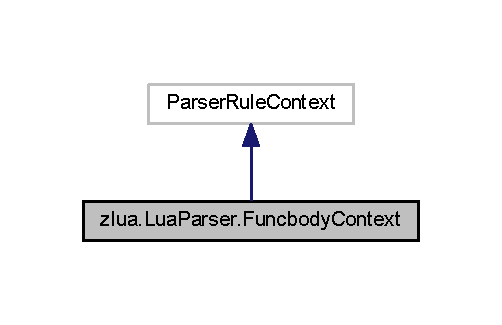
\includegraphics[width=241pt]{classzlua_1_1_lua_parser_1_1_funcbody_context__coll__graph}
\end{center}
\end{figure}
\subsection*{Public Member Functions}
\begin{DoxyCompactItemize}
\item 
\mbox{\Hypertarget{classzlua_1_1_lua_parser_1_1_funcbody_context_a3f69ad46870981aca87d790ddaa8cd7f}\label{classzlua_1_1_lua_parser_1_1_funcbody_context_a3f69ad46870981aca87d790ddaa8cd7f}} 
\mbox{\hyperlink{classzlua_1_1_lua_parser_1_1_block_context}{Block\+Context}} {\bfseries block} ()
\item 
\mbox{\Hypertarget{classzlua_1_1_lua_parser_1_1_funcbody_context_a29787d86716bb5df803d4f512b93d370}\label{classzlua_1_1_lua_parser_1_1_funcbody_context_a29787d86716bb5df803d4f512b93d370}} 
\mbox{\hyperlink{classzlua_1_1_lua_parser_1_1_parlist_context}{Parlist\+Context}} {\bfseries parlist} ()
\item 
\mbox{\Hypertarget{classzlua_1_1_lua_parser_1_1_funcbody_context_a4154d9a6704cfe985d564910d7f5eb71}\label{classzlua_1_1_lua_parser_1_1_funcbody_context_a4154d9a6704cfe985d564910d7f5eb71}} 
{\bfseries Funcbody\+Context} (Parser\+Rule\+Context parent, int invoking\+State)
\item 
\mbox{\Hypertarget{classzlua_1_1_lua_parser_1_1_funcbody_context_a54832b924cfb9091ad90c6a8167f46dd}\label{classzlua_1_1_lua_parser_1_1_funcbody_context_a54832b924cfb9091ad90c6a8167f46dd}} 
override void {\bfseries Enter\+Rule} (I\+Parse\+Tree\+Listener listener)
\item 
\mbox{\Hypertarget{classzlua_1_1_lua_parser_1_1_funcbody_context_a03414364c7a6d8fa5fff2fa2fea52205}\label{classzlua_1_1_lua_parser_1_1_funcbody_context_a03414364c7a6d8fa5fff2fa2fea52205}} 
override void {\bfseries Exit\+Rule} (I\+Parse\+Tree\+Listener listener)
\item 
\mbox{\Hypertarget{classzlua_1_1_lua_parser_1_1_funcbody_context_a8b14cb504854f8a33c2cb6fc0c07d616}\label{classzlua_1_1_lua_parser_1_1_funcbody_context_a8b14cb504854f8a33c2cb6fc0c07d616}} 
override T\+Result {\bfseries Accept$<$ T\+Result $>$} (I\+Parse\+Tree\+Visitor$<$ T\+Result $>$ visitor)
\end{DoxyCompactItemize}
\subsection*{Properties}
\begin{DoxyCompactItemize}
\item 
\mbox{\Hypertarget{classzlua_1_1_lua_parser_1_1_funcbody_context_ae3d9ab54c49a27356818861f9435d955}\label{classzlua_1_1_lua_parser_1_1_funcbody_context_ae3d9ab54c49a27356818861f9435d955}} 
override int {\bfseries Rule\+Index}\hspace{0.3cm}{\ttfamily  \mbox{[}get\mbox{]}}
\end{DoxyCompactItemize}


The documentation for this class was generated from the following file\+:\begin{DoxyCompactItemize}
\item 
zlua/Lua\+Parser.\+cs\end{DoxyCompactItemize}

\hypertarget{classzlua_1_1_lua_parser_1_1_funcname_context}{}\section{zlua.\+Lua\+Parser.\+Funcname\+Context Class Reference}
\label{classzlua_1_1_lua_parser_1_1_funcname_context}\index{zlua.\+Lua\+Parser.\+Funcname\+Context@{zlua.\+Lua\+Parser.\+Funcname\+Context}}


Inheritance diagram for zlua.\+Lua\+Parser.\+Funcname\+Context\+:
\nopagebreak
\begin{figure}[H]
\begin{center}
\leavevmode
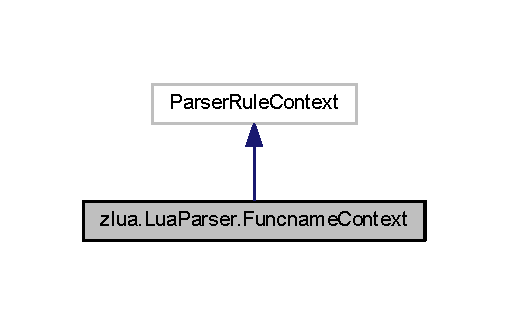
\includegraphics[width=244pt]{classzlua_1_1_lua_parser_1_1_funcname_context__inherit__graph}
\end{center}
\end{figure}


Collaboration diagram for zlua.\+Lua\+Parser.\+Funcname\+Context\+:
\nopagebreak
\begin{figure}[H]
\begin{center}
\leavevmode
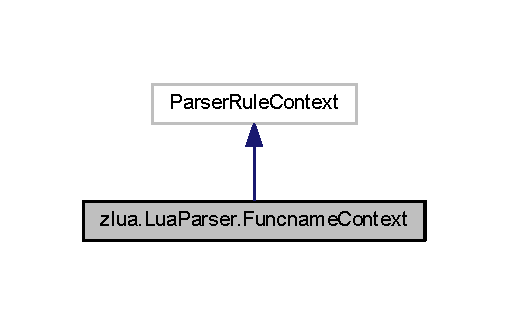
\includegraphics[width=244pt]{classzlua_1_1_lua_parser_1_1_funcname_context__coll__graph}
\end{center}
\end{figure}
\subsection*{Public Member Functions}
\begin{DoxyCompactItemize}
\item 
\mbox{\Hypertarget{classzlua_1_1_lua_parser_1_1_funcname_context_a92257512d984b112ffc473fd8508b8e9}\label{classzlua_1_1_lua_parser_1_1_funcname_context_a92257512d984b112ffc473fd8508b8e9}} 
I\+Terminal\+Node \mbox{[}$\,$\mbox{]} {\bfseries N\+A\+ME} ()
\item 
\mbox{\Hypertarget{classzlua_1_1_lua_parser_1_1_funcname_context_aca55bf4ce61abdba4b2a30ba1b5b5ae5}\label{classzlua_1_1_lua_parser_1_1_funcname_context_aca55bf4ce61abdba4b2a30ba1b5b5ae5}} 
I\+Terminal\+Node {\bfseries N\+A\+ME} (int i)
\item 
\mbox{\Hypertarget{classzlua_1_1_lua_parser_1_1_funcname_context_aa3e64bd20d2e1199df19481b98dcee54}\label{classzlua_1_1_lua_parser_1_1_funcname_context_aa3e64bd20d2e1199df19481b98dcee54}} 
{\bfseries Funcname\+Context} (Parser\+Rule\+Context parent, int invoking\+State)
\item 
\mbox{\Hypertarget{classzlua_1_1_lua_parser_1_1_funcname_context_a54fcf67e38b2d30afa22a30f7509d999}\label{classzlua_1_1_lua_parser_1_1_funcname_context_a54fcf67e38b2d30afa22a30f7509d999}} 
override void {\bfseries Enter\+Rule} (I\+Parse\+Tree\+Listener listener)
\item 
\mbox{\Hypertarget{classzlua_1_1_lua_parser_1_1_funcname_context_ace356b9f3c3fd7b1643e209208c42ab1}\label{classzlua_1_1_lua_parser_1_1_funcname_context_ace356b9f3c3fd7b1643e209208c42ab1}} 
override void {\bfseries Exit\+Rule} (I\+Parse\+Tree\+Listener listener)
\item 
\mbox{\Hypertarget{classzlua_1_1_lua_parser_1_1_funcname_context_a0715ae0310d654c791bcaf0d008d0a86}\label{classzlua_1_1_lua_parser_1_1_funcname_context_a0715ae0310d654c791bcaf0d008d0a86}} 
override T\+Result {\bfseries Accept$<$ T\+Result $>$} (I\+Parse\+Tree\+Visitor$<$ T\+Result $>$ visitor)
\end{DoxyCompactItemize}
\subsection*{Properties}
\begin{DoxyCompactItemize}
\item 
\mbox{\Hypertarget{classzlua_1_1_lua_parser_1_1_funcname_context_a0220c16bf617c9a6994533dac6b26a6a}\label{classzlua_1_1_lua_parser_1_1_funcname_context_a0220c16bf617c9a6994533dac6b26a6a}} 
override int {\bfseries Rule\+Index}\hspace{0.3cm}{\ttfamily  \mbox{[}get\mbox{]}}
\end{DoxyCompactItemize}


The documentation for this class was generated from the following file\+:\begin{DoxyCompactItemize}
\item 
zlua/Lua\+Parser.\+cs\end{DoxyCompactItemize}

\hypertarget{classzlua_1_1_lua_parser_1_1_functioncall_context}{}\section{zlua.\+Lua\+Parser.\+Functioncall\+Context Class Reference}
\label{classzlua_1_1_lua_parser_1_1_functioncall_context}\index{zlua.\+Lua\+Parser.\+Functioncall\+Context@{zlua.\+Lua\+Parser.\+Functioncall\+Context}}


Inheritance diagram for zlua.\+Lua\+Parser.\+Functioncall\+Context\+:
\nopagebreak
\begin{figure}[H]
\begin{center}
\leavevmode
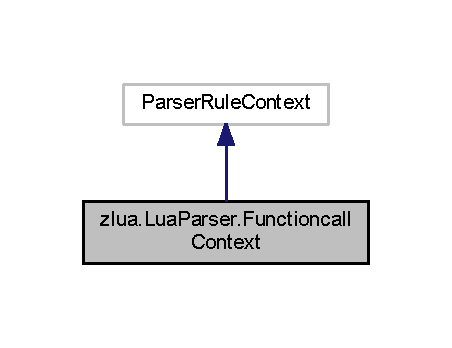
\includegraphics[width=217pt]{classzlua_1_1_lua_parser_1_1_functioncall_context__inherit__graph}
\end{center}
\end{figure}


Collaboration diagram for zlua.\+Lua\+Parser.\+Functioncall\+Context\+:
\nopagebreak
\begin{figure}[H]
\begin{center}
\leavevmode
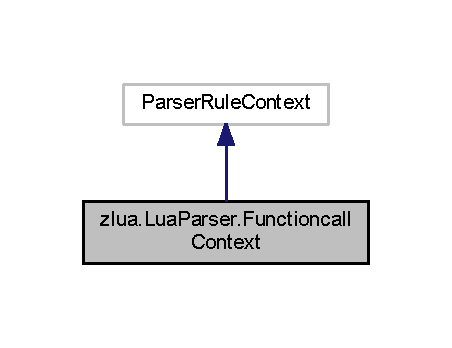
\includegraphics[width=217pt]{classzlua_1_1_lua_parser_1_1_functioncall_context__coll__graph}
\end{center}
\end{figure}
\subsection*{Public Member Functions}
\begin{DoxyCompactItemize}
\item 
\mbox{\Hypertarget{classzlua_1_1_lua_parser_1_1_functioncall_context_a4e2acf6c90255d632a65bb075b538554}\label{classzlua_1_1_lua_parser_1_1_functioncall_context_a4e2acf6c90255d632a65bb075b538554}} 
\mbox{\hyperlink{classzlua_1_1_lua_parser_1_1_var_or_exp_context}{Var\+Or\+Exp\+Context}} {\bfseries var\+Or\+Exp} ()
\item 
\mbox{\Hypertarget{classzlua_1_1_lua_parser_1_1_functioncall_context_a41aeb4e095435d6ec7fc25f5d6520875}\label{classzlua_1_1_lua_parser_1_1_functioncall_context_a41aeb4e095435d6ec7fc25f5d6520875}} 
\mbox{\hyperlink{classzlua_1_1_lua_parser_1_1_name_and_args_context}{Name\+And\+Args\+Context}} \mbox{[}$\,$\mbox{]} {\bfseries name\+And\+Args} ()
\item 
\mbox{\Hypertarget{classzlua_1_1_lua_parser_1_1_functioncall_context_a946850fdebae4f9a1d5262f0ee254fea}\label{classzlua_1_1_lua_parser_1_1_functioncall_context_a946850fdebae4f9a1d5262f0ee254fea}} 
\mbox{\hyperlink{classzlua_1_1_lua_parser_1_1_name_and_args_context}{Name\+And\+Args\+Context}} {\bfseries name\+And\+Args} (int i)
\item 
\mbox{\Hypertarget{classzlua_1_1_lua_parser_1_1_functioncall_context_a0cc61367967c5893883a5d798dcd0449}\label{classzlua_1_1_lua_parser_1_1_functioncall_context_a0cc61367967c5893883a5d798dcd0449}} 
{\bfseries Functioncall\+Context} (Parser\+Rule\+Context parent, int invoking\+State)
\item 
\mbox{\Hypertarget{classzlua_1_1_lua_parser_1_1_functioncall_context_a5e13cc76081cd0e42d6a84f8c85d9542}\label{classzlua_1_1_lua_parser_1_1_functioncall_context_a5e13cc76081cd0e42d6a84f8c85d9542}} 
override void {\bfseries Enter\+Rule} (I\+Parse\+Tree\+Listener listener)
\item 
\mbox{\Hypertarget{classzlua_1_1_lua_parser_1_1_functioncall_context_a9c9506792fc7ae68f7a069ef03651c62}\label{classzlua_1_1_lua_parser_1_1_functioncall_context_a9c9506792fc7ae68f7a069ef03651c62}} 
override void {\bfseries Exit\+Rule} (I\+Parse\+Tree\+Listener listener)
\item 
\mbox{\Hypertarget{classzlua_1_1_lua_parser_1_1_functioncall_context_a65b5ed4b733c1fc9788fcd78620a95a6}\label{classzlua_1_1_lua_parser_1_1_functioncall_context_a65b5ed4b733c1fc9788fcd78620a95a6}} 
override T\+Result {\bfseries Accept$<$ T\+Result $>$} (I\+Parse\+Tree\+Visitor$<$ T\+Result $>$ visitor)
\end{DoxyCompactItemize}
\subsection*{Properties}
\begin{DoxyCompactItemize}
\item 
\mbox{\Hypertarget{classzlua_1_1_lua_parser_1_1_functioncall_context_ae1af108cddeb88de50de99458da0d85f}\label{classzlua_1_1_lua_parser_1_1_functioncall_context_ae1af108cddeb88de50de99458da0d85f}} 
override int {\bfseries Rule\+Index}\hspace{0.3cm}{\ttfamily  \mbox{[}get\mbox{]}}
\end{DoxyCompactItemize}


The documentation for this class was generated from the following file\+:\begin{DoxyCompactItemize}
\item 
zlua/Lua\+Parser.\+cs\end{DoxyCompactItemize}

\hypertarget{classzlua_1_1_lua_parser_1_1_functiondef_context}{}\section{zlua.\+Lua\+Parser.\+Functiondef\+Context Class Reference}
\label{classzlua_1_1_lua_parser_1_1_functiondef_context}\index{zlua.\+Lua\+Parser.\+Functiondef\+Context@{zlua.\+Lua\+Parser.\+Functiondef\+Context}}


Inheritance diagram for zlua.\+Lua\+Parser.\+Functiondef\+Context\+:
\nopagebreak
\begin{figure}[H]
\begin{center}
\leavevmode
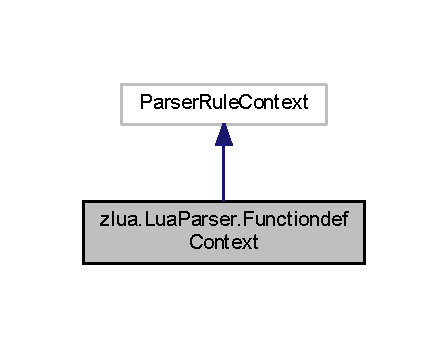
\includegraphics[width=215pt]{classzlua_1_1_lua_parser_1_1_functiondef_context__inherit__graph}
\end{center}
\end{figure}


Collaboration diagram for zlua.\+Lua\+Parser.\+Functiondef\+Context\+:
\nopagebreak
\begin{figure}[H]
\begin{center}
\leavevmode
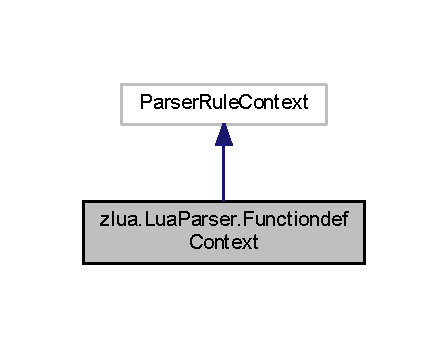
\includegraphics[width=215pt]{classzlua_1_1_lua_parser_1_1_functiondef_context__coll__graph}
\end{center}
\end{figure}
\subsection*{Public Member Functions}
\begin{DoxyCompactItemize}
\item 
\mbox{\Hypertarget{classzlua_1_1_lua_parser_1_1_functiondef_context_a87f0da9372f14f1a32cee0f30b880cf3}\label{classzlua_1_1_lua_parser_1_1_functiondef_context_a87f0da9372f14f1a32cee0f30b880cf3}} 
\mbox{\hyperlink{classzlua_1_1_lua_parser_1_1_funcbody_context}{Funcbody\+Context}} {\bfseries funcbody} ()
\item 
\mbox{\Hypertarget{classzlua_1_1_lua_parser_1_1_functiondef_context_a100661ed3994f15b5a612166d56f6523}\label{classzlua_1_1_lua_parser_1_1_functiondef_context_a100661ed3994f15b5a612166d56f6523}} 
{\bfseries Functiondef\+Context} (Parser\+Rule\+Context parent, int invoking\+State)
\item 
\mbox{\Hypertarget{classzlua_1_1_lua_parser_1_1_functiondef_context_af57ac3aa90ad102d98f550c13b258db1}\label{classzlua_1_1_lua_parser_1_1_functiondef_context_af57ac3aa90ad102d98f550c13b258db1}} 
override void {\bfseries Enter\+Rule} (I\+Parse\+Tree\+Listener listener)
\item 
\mbox{\Hypertarget{classzlua_1_1_lua_parser_1_1_functiondef_context_acf6f364f0a0bfe6b6f8b46d2b19f1ba4}\label{classzlua_1_1_lua_parser_1_1_functiondef_context_acf6f364f0a0bfe6b6f8b46d2b19f1ba4}} 
override void {\bfseries Exit\+Rule} (I\+Parse\+Tree\+Listener listener)
\item 
\mbox{\Hypertarget{classzlua_1_1_lua_parser_1_1_functiondef_context_a6ac70448dad6b4940b6f5f32591a8349}\label{classzlua_1_1_lua_parser_1_1_functiondef_context_a6ac70448dad6b4940b6f5f32591a8349}} 
override T\+Result {\bfseries Accept$<$ T\+Result $>$} (I\+Parse\+Tree\+Visitor$<$ T\+Result $>$ visitor)
\end{DoxyCompactItemize}
\subsection*{Properties}
\begin{DoxyCompactItemize}
\item 
\mbox{\Hypertarget{classzlua_1_1_lua_parser_1_1_functiondef_context_a4ad1b35a2721c9bb09ca4a86aeaefe35}\label{classzlua_1_1_lua_parser_1_1_functiondef_context_a4ad1b35a2721c9bb09ca4a86aeaefe35}} 
override int {\bfseries Rule\+Index}\hspace{0.3cm}{\ttfamily  \mbox{[}get\mbox{]}}
\end{DoxyCompactItemize}


The documentation for this class was generated from the following file\+:\begin{DoxyCompactItemize}
\item 
zlua/Lua\+Parser.\+cs\end{DoxyCompactItemize}

\hypertarget{classzlua_1_1_lua_1_1_g_c_object}{}\section{zlua.\+Lua.\+G\+C\+Object Class Reference}
\label{classzlua_1_1_lua_1_1_g_c_object}\index{zlua.\+Lua.\+G\+C\+Object@{zlua.\+Lua.\+G\+C\+Object}}


(C\# simulated) union of GC objects how it simulates union\+: polymorphic  




Inheritance diagram for zlua.\+Lua.\+G\+C\+Object\+:
\nopagebreak
\begin{figure}[H]
\begin{center}
\leavevmode
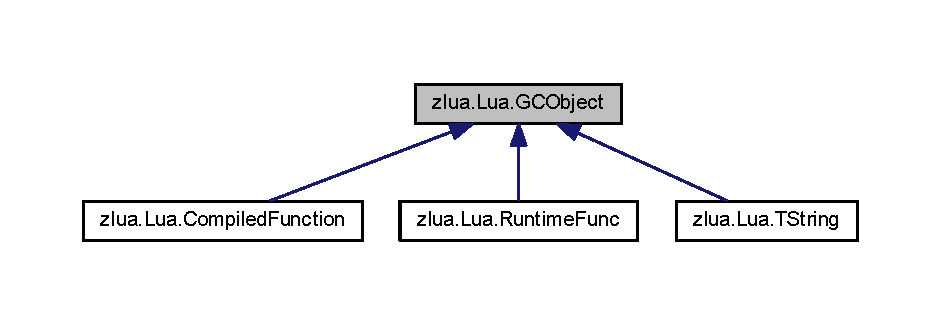
\includegraphics[width=350pt]{classzlua_1_1_lua_1_1_g_c_object__inherit__graph}
\end{center}
\end{figure}
\subsection*{Properties}
\begin{DoxyCompactItemize}
\item 
\mbox{\hyperlink{classzlua_1_1_lua_1_1_t_string}{T\+String}} \mbox{\hyperlink{classzlua_1_1_lua_1_1_g_c_object_adb3aafad7ab9791defdd09ddb5f56d64}{tstring}}\hspace{0.3cm}{\ttfamily  \mbox{[}get\mbox{]}}
\begin{DoxyCompactList}\small\item\em for convenience (eg. \mbox{\hyperlink{classzlua_1_1_lua_1_1_t_string}{T\+String}} is subclass of G\+C\+Object) \end{DoxyCompactList}\item 
\mbox{\Hypertarget{classzlua_1_1_lua_1_1_g_c_object_af737475ae9f265e594bc78adef201ff8}\label{classzlua_1_1_lua_1_1_g_c_object_af737475ae9f265e594bc78adef201ff8}} 
\mbox{\hyperlink{classzlua_1_1_lua_1_1_compiled_function}{Compiled\+Function}} {\bfseries compiled\+\_\+func}\hspace{0.3cm}{\ttfamily  \mbox{[}get\mbox{]}}
\item 
\mbox{\Hypertarget{classzlua_1_1_lua_1_1_g_c_object_a3e1ac4cb8e5ee80c17e680c7aa6e0cdb}\label{classzlua_1_1_lua_1_1_g_c_object_a3e1ac4cb8e5ee80c17e680c7aa6e0cdb}} 
\mbox{\hyperlink{classzlua_1_1_lua_1_1_runtime_func}{Runtime\+Func}} {\bfseries runtime\+\_\+func}\hspace{0.3cm}{\ttfamily  \mbox{[}get\mbox{]}}
\end{DoxyCompactItemize}


\subsection{Detailed Description}
(C\# simulated) union of GC objects how it simulates union\+: polymorphic 


\begin{DoxyEnumerate}
\item inheritance graph\+: G\+Cheader $>$ \mbox{\hyperlink{classzlua_1_1_lua_1_1_g_c_object}{G\+C\+Object}} $>$ \mbox{\hyperlink{classzlua_1_1_lua_1_1_t_string}{T\+String}}, Udata ... (all GC types of lua)
\item \mbox{\hyperlink{classzlua_1_1_lua_1_1_g_c_object}{G\+C\+Object}} use property to return specific type of value with polymorphic 
\end{DoxyEnumerate}

\subsection{Property Documentation}
\mbox{\Hypertarget{classzlua_1_1_lua_1_1_g_c_object_adb3aafad7ab9791defdd09ddb5f56d64}\label{classzlua_1_1_lua_1_1_g_c_object_adb3aafad7ab9791defdd09ddb5f56d64}} 
\index{zlua\+::\+Lua\+::\+G\+C\+Object@{zlua\+::\+Lua\+::\+G\+C\+Object}!tstring@{tstring}}
\index{tstring@{tstring}!zlua\+::\+Lua\+::\+G\+C\+Object@{zlua\+::\+Lua\+::\+G\+C\+Object}}
\subsubsection{\texorpdfstring{tstring}{tstring}}
{\footnotesize\ttfamily \mbox{\hyperlink{classzlua_1_1_lua_1_1_t_string}{T\+String}} zlua.\+Lua.\+G\+C\+Object.\+tstring\hspace{0.3cm}{\ttfamily [get]}}



for convenience (eg. \mbox{\hyperlink{classzlua_1_1_lua_1_1_t_string}{T\+String}} is subclass of G\+C\+Object) 



The documentation for this class was generated from the following file\+:\begin{DoxyCompactItemize}
\item 
zlua/lobject.\+cs\end{DoxyCompactItemize}

\hypertarget{classzlua_1_1_lua_parser_1_1_global__func__def__stat_context}{}\section{zlua.\+Lua\+Parser.\+Global\+\_\+func\+\_\+def\+\_\+stat\+Context Class Reference}
\label{classzlua_1_1_lua_parser_1_1_global__func__def__stat_context}\index{zlua.\+Lua\+Parser.\+Global\+\_\+func\+\_\+def\+\_\+stat\+Context@{zlua.\+Lua\+Parser.\+Global\+\_\+func\+\_\+def\+\_\+stat\+Context}}


Inheritance diagram for zlua.\+Lua\+Parser.\+Global\+\_\+func\+\_\+def\+\_\+stat\+Context\+:
\nopagebreak
\begin{figure}[H]
\begin{center}
\leavevmode
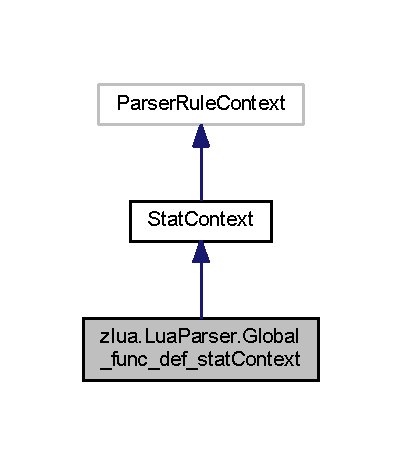
\includegraphics[width=193pt]{classzlua_1_1_lua_parser_1_1_global__func__def__stat_context__inherit__graph}
\end{center}
\end{figure}


Collaboration diagram for zlua.\+Lua\+Parser.\+Global\+\_\+func\+\_\+def\+\_\+stat\+Context\+:
\nopagebreak
\begin{figure}[H]
\begin{center}
\leavevmode
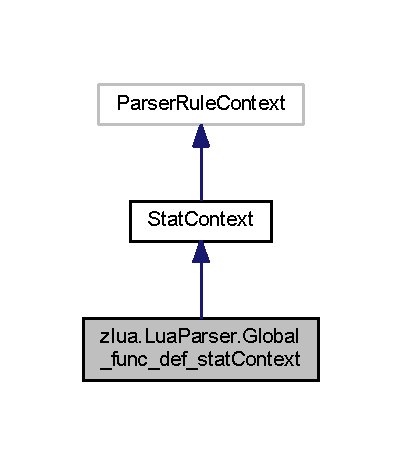
\includegraphics[width=193pt]{classzlua_1_1_lua_parser_1_1_global__func__def__stat_context__coll__graph}
\end{center}
\end{figure}
\subsection*{Public Member Functions}
\begin{DoxyCompactItemize}
\item 
\mbox{\Hypertarget{classzlua_1_1_lua_parser_1_1_global__func__def__stat_context_a31f90896b81a2a28d6b66eaff2f43ff5}\label{classzlua_1_1_lua_parser_1_1_global__func__def__stat_context_a31f90896b81a2a28d6b66eaff2f43ff5}} 
I\+Terminal\+Node {\bfseries N\+A\+ME} ()
\item 
\mbox{\Hypertarget{classzlua_1_1_lua_parser_1_1_global__func__def__stat_context_a2cadca10c4f416916ca925cd88b86f98}\label{classzlua_1_1_lua_parser_1_1_global__func__def__stat_context_a2cadca10c4f416916ca925cd88b86f98}} 
\mbox{\hyperlink{classzlua_1_1_lua_parser_1_1_funcbody_context}{Funcbody\+Context}} {\bfseries funcbody} ()
\item 
\mbox{\Hypertarget{classzlua_1_1_lua_parser_1_1_global__func__def__stat_context_af2988c25b7f5406446d70c7cdbfdf44b}\label{classzlua_1_1_lua_parser_1_1_global__func__def__stat_context_af2988c25b7f5406446d70c7cdbfdf44b}} 
{\bfseries Global\+\_\+func\+\_\+def\+\_\+stat\+Context} (\mbox{\hyperlink{classzlua_1_1_lua_parser_1_1_stat_context}{Stat\+Context}} context)
\item 
\mbox{\Hypertarget{classzlua_1_1_lua_parser_1_1_global__func__def__stat_context_a6253a97793b43947e98a072d107ad865}\label{classzlua_1_1_lua_parser_1_1_global__func__def__stat_context_a6253a97793b43947e98a072d107ad865}} 
override void {\bfseries Enter\+Rule} (I\+Parse\+Tree\+Listener listener)
\item 
\mbox{\Hypertarget{classzlua_1_1_lua_parser_1_1_global__func__def__stat_context_ac5ab079cb34c61bfa3b741fd9a598387}\label{classzlua_1_1_lua_parser_1_1_global__func__def__stat_context_ac5ab079cb34c61bfa3b741fd9a598387}} 
override void {\bfseries Exit\+Rule} (I\+Parse\+Tree\+Listener listener)
\item 
\mbox{\Hypertarget{classzlua_1_1_lua_parser_1_1_global__func__def__stat_context_ae5d455bf3e389df7413e1ca4b7c9a809}\label{classzlua_1_1_lua_parser_1_1_global__func__def__stat_context_ae5d455bf3e389df7413e1ca4b7c9a809}} 
override T\+Result {\bfseries Accept$<$ T\+Result $>$} (I\+Parse\+Tree\+Visitor$<$ T\+Result $>$ visitor)
\end{DoxyCompactItemize}
\subsection*{Additional Inherited Members}


The documentation for this class was generated from the following file\+:\begin{DoxyCompactItemize}
\item 
zlua/Lua\+Parser.\+cs\end{DoxyCompactItemize}

\hypertarget{classzlua_1_1_lua_parser_1_1_global__var__stat_context}{}\section{zlua.\+Lua\+Parser.\+Global\+\_\+var\+\_\+stat\+Context Class Reference}
\label{classzlua_1_1_lua_parser_1_1_global__var__stat_context}\index{zlua.\+Lua\+Parser.\+Global\+\_\+var\+\_\+stat\+Context@{zlua.\+Lua\+Parser.\+Global\+\_\+var\+\_\+stat\+Context}}


Inheritance diagram for zlua.\+Lua\+Parser.\+Global\+\_\+var\+\_\+stat\+Context\+:
\nopagebreak
\begin{figure}[H]
\begin{center}
\leavevmode
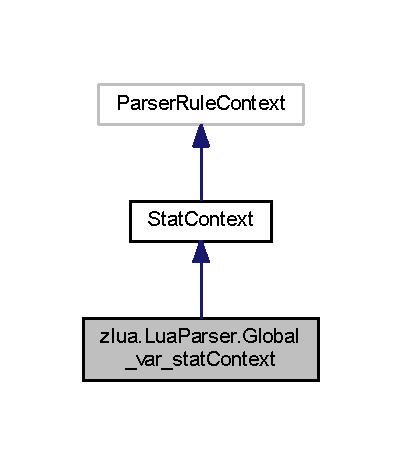
\includegraphics[width=193pt]{classzlua_1_1_lua_parser_1_1_global__var__stat_context__inherit__graph}
\end{center}
\end{figure}


Collaboration diagram for zlua.\+Lua\+Parser.\+Global\+\_\+var\+\_\+stat\+Context\+:
\nopagebreak
\begin{figure}[H]
\begin{center}
\leavevmode
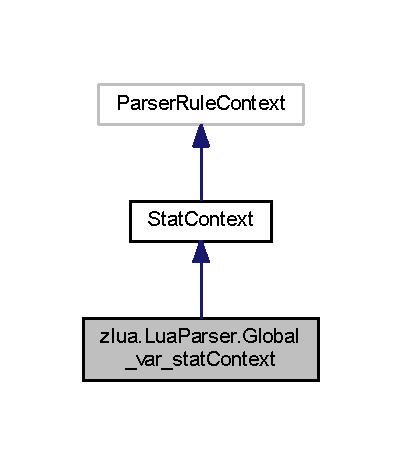
\includegraphics[width=193pt]{classzlua_1_1_lua_parser_1_1_global__var__stat_context__coll__graph}
\end{center}
\end{figure}
\subsection*{Public Member Functions}
\begin{DoxyCompactItemize}
\item 
\mbox{\Hypertarget{classzlua_1_1_lua_parser_1_1_global__var__stat_context_ab3995e184a34af0164126cfd9dc9b930}\label{classzlua_1_1_lua_parser_1_1_global__var__stat_context_ab3995e184a34af0164126cfd9dc9b930}} 
\mbox{\hyperlink{classzlua_1_1_lua_parser_1_1_var_context}{Var\+Context}} {\bfseries var} ()
\item 
\mbox{\Hypertarget{classzlua_1_1_lua_parser_1_1_global__var__stat_context_a800e7a2aadee1e1e7193393f3d6603e9}\label{classzlua_1_1_lua_parser_1_1_global__var__stat_context_a800e7a2aadee1e1e7193393f3d6603e9}} 
\mbox{\hyperlink{classzlua_1_1_lua_parser_1_1_exp_context}{Exp\+Context}} {\bfseries exp} ()
\item 
\mbox{\Hypertarget{classzlua_1_1_lua_parser_1_1_global__var__stat_context_a93d4c3b82a8e289402cb758715acbe42}\label{classzlua_1_1_lua_parser_1_1_global__var__stat_context_a93d4c3b82a8e289402cb758715acbe42}} 
{\bfseries Global\+\_\+var\+\_\+stat\+Context} (\mbox{\hyperlink{classzlua_1_1_lua_parser_1_1_stat_context}{Stat\+Context}} context)
\item 
\mbox{\Hypertarget{classzlua_1_1_lua_parser_1_1_global__var__stat_context_afd37a410a364103b506ce82b12001cca}\label{classzlua_1_1_lua_parser_1_1_global__var__stat_context_afd37a410a364103b506ce82b12001cca}} 
override void {\bfseries Enter\+Rule} (I\+Parse\+Tree\+Listener listener)
\item 
\mbox{\Hypertarget{classzlua_1_1_lua_parser_1_1_global__var__stat_context_a8f03da53bf7a6146ed39747adac9f21b}\label{classzlua_1_1_lua_parser_1_1_global__var__stat_context_a8f03da53bf7a6146ed39747adac9f21b}} 
override void {\bfseries Exit\+Rule} (I\+Parse\+Tree\+Listener listener)
\item 
\mbox{\Hypertarget{classzlua_1_1_lua_parser_1_1_global__var__stat_context_a55a80470346308b091d2561a9f28756c}\label{classzlua_1_1_lua_parser_1_1_global__var__stat_context_a55a80470346308b091d2561a9f28756c}} 
override T\+Result {\bfseries Accept$<$ T\+Result $>$} (I\+Parse\+Tree\+Visitor$<$ T\+Result $>$ visitor)
\end{DoxyCompactItemize}
\subsection*{Additional Inherited Members}


The documentation for this class was generated from the following file\+:\begin{DoxyCompactItemize}
\item 
zlua/Lua\+Parser.\+cs\end{DoxyCompactItemize}

\hypertarget{classzlua_1_1_lua_parser_1_1_if__stat_context}{}\section{zlua.\+Lua\+Parser.\+If\+\_\+stat\+Context Class Reference}
\label{classzlua_1_1_lua_parser_1_1_if__stat_context}\index{zlua.\+Lua\+Parser.\+If\+\_\+stat\+Context@{zlua.\+Lua\+Parser.\+If\+\_\+stat\+Context}}


Inheritance diagram for zlua.\+Lua\+Parser.\+If\+\_\+stat\+Context\+:
\nopagebreak
\begin{figure}[H]
\begin{center}
\leavevmode
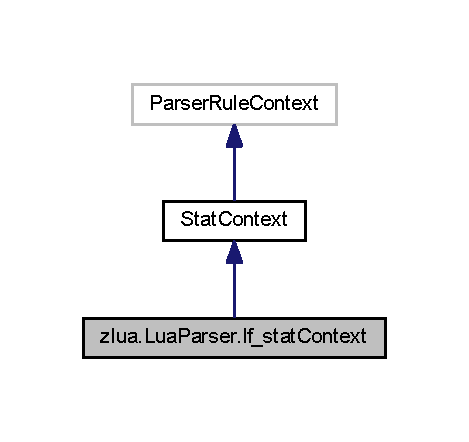
\includegraphics[width=225pt]{classzlua_1_1_lua_parser_1_1_if__stat_context__inherit__graph}
\end{center}
\end{figure}


Collaboration diagram for zlua.\+Lua\+Parser.\+If\+\_\+stat\+Context\+:
\nopagebreak
\begin{figure}[H]
\begin{center}
\leavevmode
\includegraphics[width=225pt]{classzlua_1_1_lua_parser_1_1_if__stat_context__coll__graph}
\end{center}
\end{figure}
\subsection*{Public Member Functions}
\begin{DoxyCompactItemize}
\item 
\mbox{\Hypertarget{classzlua_1_1_lua_parser_1_1_if__stat_context_a0da79211b10ac5ee2bfcb765928d1acc}\label{classzlua_1_1_lua_parser_1_1_if__stat_context_a0da79211b10ac5ee2bfcb765928d1acc}} 
\mbox{\hyperlink{classzlua_1_1_lua_parser_1_1_exp_context}{Exp\+Context}} \mbox{[}$\,$\mbox{]} {\bfseries exp} ()
\item 
\mbox{\Hypertarget{classzlua_1_1_lua_parser_1_1_if__stat_context_a304e6c662af48191688282f906caa73b}\label{classzlua_1_1_lua_parser_1_1_if__stat_context_a304e6c662af48191688282f906caa73b}} 
\mbox{\hyperlink{classzlua_1_1_lua_parser_1_1_exp_context}{Exp\+Context}} {\bfseries exp} (int i)
\item 
\mbox{\Hypertarget{classzlua_1_1_lua_parser_1_1_if__stat_context_ae6753b67c59fbf3f07fc0edc45041bb8}\label{classzlua_1_1_lua_parser_1_1_if__stat_context_ae6753b67c59fbf3f07fc0edc45041bb8}} 
\mbox{\hyperlink{classzlua_1_1_lua_parser_1_1_block_context}{Block\+Context}} \mbox{[}$\,$\mbox{]} {\bfseries block} ()
\item 
\mbox{\Hypertarget{classzlua_1_1_lua_parser_1_1_if__stat_context_aea069f59d24bbb1d00d473451e14b3cb}\label{classzlua_1_1_lua_parser_1_1_if__stat_context_aea069f59d24bbb1d00d473451e14b3cb}} 
\mbox{\hyperlink{classzlua_1_1_lua_parser_1_1_block_context}{Block\+Context}} {\bfseries block} (int i)
\item 
\mbox{\Hypertarget{classzlua_1_1_lua_parser_1_1_if__stat_context_a53d7baaaa3a1dacf428b67c14c57246f}\label{classzlua_1_1_lua_parser_1_1_if__stat_context_a53d7baaaa3a1dacf428b67c14c57246f}} 
{\bfseries If\+\_\+stat\+Context} (\mbox{\hyperlink{classzlua_1_1_lua_parser_1_1_stat_context}{Stat\+Context}} context)
\item 
\mbox{\Hypertarget{classzlua_1_1_lua_parser_1_1_if__stat_context_ac6693fa0843352feee5fe2438d02e588}\label{classzlua_1_1_lua_parser_1_1_if__stat_context_ac6693fa0843352feee5fe2438d02e588}} 
override void {\bfseries Enter\+Rule} (I\+Parse\+Tree\+Listener listener)
\item 
\mbox{\Hypertarget{classzlua_1_1_lua_parser_1_1_if__stat_context_ad6879a4f8782a9d074ff8fb7fce9ed61}\label{classzlua_1_1_lua_parser_1_1_if__stat_context_ad6879a4f8782a9d074ff8fb7fce9ed61}} 
override void {\bfseries Exit\+Rule} (I\+Parse\+Tree\+Listener listener)
\item 
\mbox{\Hypertarget{classzlua_1_1_lua_parser_1_1_if__stat_context_a5501fb0f4d586bb671b61290b7efa4e3}\label{classzlua_1_1_lua_parser_1_1_if__stat_context_a5501fb0f4d586bb671b61290b7efa4e3}} 
override T\+Result {\bfseries Accept$<$ T\+Result $>$} (I\+Parse\+Tree\+Visitor$<$ T\+Result $>$ visitor)
\end{DoxyCompactItemize}
\subsection*{Additional Inherited Members}


The documentation for this class was generated from the following file\+:\begin{DoxyCompactItemize}
\item 
zlua/Lua\+Parser.\+cs\end{DoxyCompactItemize}

\hypertarget{interfacezlua_1_1_i_lua_listener}{}\section{zlua.\+I\+Lua\+Listener Interface Reference}
\label{interfacezlua_1_1_i_lua_listener}\index{zlua.\+I\+Lua\+Listener@{zlua.\+I\+Lua\+Listener}}


This interface defines a complete listener for a parse tree produced by \mbox{\hyperlink{classzlua_1_1_lua_parser}{Lua\+Parser}}.  




Inheritance diagram for zlua.\+I\+Lua\+Listener\+:
\nopagebreak
\begin{figure}[H]
\begin{center}
\leavevmode
\includegraphics[width=284pt]{interfacezlua_1_1_i_lua_listener__inherit__graph}
\end{center}
\end{figure}


Collaboration diagram for zlua.\+I\+Lua\+Listener\+:
\nopagebreak
\begin{figure}[H]
\begin{center}
\leavevmode
\includegraphics[width=178pt]{interfacezlua_1_1_i_lua_listener__coll__graph}
\end{center}
\end{figure}
\subsection*{Public Member Functions}
\begin{DoxyCompactItemize}
\item 
void \mbox{\hyperlink{interfacezlua_1_1_i_lua_listener_aaa6652e41dd59516afb02cde17c6a347}{Enter\+Empty\+\_\+stat}} (\mbox{[}Not\+Null\mbox{]} \mbox{\hyperlink{classzlua_1_1_lua_parser_1_1_empty__stat_context}{Lua\+Parser.\+Empty\+\_\+stat\+Context}} context)
\begin{DoxyCompactList}\small\item\em Enter a parse tree produced by the {\ttfamily empty\+\_\+stat} labeled alternative in Lua\+Parser.\+stat. \end{DoxyCompactList}\item 
void \mbox{\hyperlink{interfacezlua_1_1_i_lua_listener_a5d6586f89158ceb4a9e683bbc2463ef3}{Exit\+Empty\+\_\+stat}} (\mbox{[}Not\+Null\mbox{]} \mbox{\hyperlink{classzlua_1_1_lua_parser_1_1_empty__stat_context}{Lua\+Parser.\+Empty\+\_\+stat\+Context}} context)
\begin{DoxyCompactList}\small\item\em Exit a parse tree produced by the {\ttfamily empty\+\_\+stat} labeled alternative in Lua\+Parser.\+stat. \end{DoxyCompactList}\item 
void \mbox{\hyperlink{interfacezlua_1_1_i_lua_listener_a6c89bd1b72debe5db0a3bd633af3c6c9}{Enter\+Assign\+\_\+stat}} (\mbox{[}Not\+Null\mbox{]} \mbox{\hyperlink{classzlua_1_1_lua_parser_1_1_assign__stat_context}{Lua\+Parser.\+Assign\+\_\+stat\+Context}} context)
\begin{DoxyCompactList}\small\item\em Enter a parse tree produced by the {\ttfamily assign\+\_\+stat} labeled alternative in Lua\+Parser.\+stat. \end{DoxyCompactList}\item 
void \mbox{\hyperlink{interfacezlua_1_1_i_lua_listener_ad3a0df056fe6b0c23d11cad89f6091c7}{Exit\+Assign\+\_\+stat}} (\mbox{[}Not\+Null\mbox{]} \mbox{\hyperlink{classzlua_1_1_lua_parser_1_1_assign__stat_context}{Lua\+Parser.\+Assign\+\_\+stat\+Context}} context)
\begin{DoxyCompactList}\small\item\em Exit a parse tree produced by the {\ttfamily assign\+\_\+stat} labeled alternative in Lua\+Parser.\+stat. \end{DoxyCompactList}\item 
void \mbox{\hyperlink{interfacezlua_1_1_i_lua_listener_a082ec71bf7dc3bee6dd365c9a56ee59c}{Enter\+Func\+\_\+call\+\_\+stat}} (\mbox{[}Not\+Null\mbox{]} \mbox{\hyperlink{classzlua_1_1_lua_parser_1_1_func__call__stat_context}{Lua\+Parser.\+Func\+\_\+call\+\_\+stat\+Context}} context)
\begin{DoxyCompactList}\small\item\em Enter a parse tree produced by the {\ttfamily func\+\_\+call\+\_\+stat} labeled alternative in Lua\+Parser.\+stat. \end{DoxyCompactList}\item 
void \mbox{\hyperlink{interfacezlua_1_1_i_lua_listener_ab9aba8c96896e86ec76ca5a87c5d2f25}{Exit\+Func\+\_\+call\+\_\+stat}} (\mbox{[}Not\+Null\mbox{]} \mbox{\hyperlink{classzlua_1_1_lua_parser_1_1_func__call__stat_context}{Lua\+Parser.\+Func\+\_\+call\+\_\+stat\+Context}} context)
\begin{DoxyCompactList}\small\item\em Exit a parse tree produced by the {\ttfamily func\+\_\+call\+\_\+stat} labeled alternative in Lua\+Parser.\+stat. \end{DoxyCompactList}\item 
void \mbox{\hyperlink{interfacezlua_1_1_i_lua_listener_aa77c8634ee96ca2069ceb9e93b2bae57}{Enter\+Break\+\_\+stat}} (\mbox{[}Not\+Null\mbox{]} \mbox{\hyperlink{classzlua_1_1_lua_parser_1_1_break__stat_context}{Lua\+Parser.\+Break\+\_\+stat\+Context}} context)
\begin{DoxyCompactList}\small\item\em Enter a parse tree produced by the {\ttfamily break\+\_\+stat} labeled alternative in Lua\+Parser.\+stat. \end{DoxyCompactList}\item 
void \mbox{\hyperlink{interfacezlua_1_1_i_lua_listener_a869e5a8abc4ddac071073a74bf09b6c5}{Exit\+Break\+\_\+stat}} (\mbox{[}Not\+Null\mbox{]} \mbox{\hyperlink{classzlua_1_1_lua_parser_1_1_break__stat_context}{Lua\+Parser.\+Break\+\_\+stat\+Context}} context)
\begin{DoxyCompactList}\small\item\em Exit a parse tree produced by the {\ttfamily break\+\_\+stat} labeled alternative in Lua\+Parser.\+stat. \end{DoxyCompactList}\item 
void \mbox{\hyperlink{interfacezlua_1_1_i_lua_listener_ad561e0f5feb33ca80ba5202ab0511bab}{Enter\+Do\+\_\+end\+\_\+stat}} (\mbox{[}Not\+Null\mbox{]} \mbox{\hyperlink{classzlua_1_1_lua_parser_1_1_do__end__stat_context}{Lua\+Parser.\+Do\+\_\+end\+\_\+stat\+Context}} context)
\begin{DoxyCompactList}\small\item\em Enter a parse tree produced by the {\ttfamily do\+\_\+end\+\_\+stat} labeled alternative in Lua\+Parser.\+stat. \end{DoxyCompactList}\item 
void \mbox{\hyperlink{interfacezlua_1_1_i_lua_listener_a21222197a86ad5c425dcab38204a7840}{Exit\+Do\+\_\+end\+\_\+stat}} (\mbox{[}Not\+Null\mbox{]} \mbox{\hyperlink{classzlua_1_1_lua_parser_1_1_do__end__stat_context}{Lua\+Parser.\+Do\+\_\+end\+\_\+stat\+Context}} context)
\begin{DoxyCompactList}\small\item\em Exit a parse tree produced by the {\ttfamily do\+\_\+end\+\_\+stat} labeled alternative in Lua\+Parser.\+stat. \end{DoxyCompactList}\item 
void \mbox{\hyperlink{interfacezlua_1_1_i_lua_listener_abc1fb6386fa985aa88c2813bc1040876}{Enter\+While\+\_\+stat}} (\mbox{[}Not\+Null\mbox{]} \mbox{\hyperlink{classzlua_1_1_lua_parser_1_1_while__stat_context}{Lua\+Parser.\+While\+\_\+stat\+Context}} context)
\begin{DoxyCompactList}\small\item\em Enter a parse tree produced by the {\ttfamily while\+\_\+stat} labeled alternative in Lua\+Parser.\+stat. \end{DoxyCompactList}\item 
void \mbox{\hyperlink{interfacezlua_1_1_i_lua_listener_ab7cdf0dd588b664e1f8efbca0a03884e}{Exit\+While\+\_\+stat}} (\mbox{[}Not\+Null\mbox{]} \mbox{\hyperlink{classzlua_1_1_lua_parser_1_1_while__stat_context}{Lua\+Parser.\+While\+\_\+stat\+Context}} context)
\begin{DoxyCompactList}\small\item\em Exit a parse tree produced by the {\ttfamily while\+\_\+stat} labeled alternative in Lua\+Parser.\+stat. \end{DoxyCompactList}\item 
void \mbox{\hyperlink{interfacezlua_1_1_i_lua_listener_ae4466707d78b9bb5f5836ed8710e4ef1}{Enter\+If\+\_\+stat}} (\mbox{[}Not\+Null\mbox{]} \mbox{\hyperlink{classzlua_1_1_lua_parser_1_1_if__stat_context}{Lua\+Parser.\+If\+\_\+stat\+Context}} context)
\begin{DoxyCompactList}\small\item\em Enter a parse tree produced by the {\ttfamily if\+\_\+stat} labeled alternative in Lua\+Parser.\+stat. \end{DoxyCompactList}\item 
void \mbox{\hyperlink{interfacezlua_1_1_i_lua_listener_a2f0389129d1846cafed21b068ecdb15d}{Exit\+If\+\_\+stat}} (\mbox{[}Not\+Null\mbox{]} \mbox{\hyperlink{classzlua_1_1_lua_parser_1_1_if__stat_context}{Lua\+Parser.\+If\+\_\+stat\+Context}} context)
\begin{DoxyCompactList}\small\item\em Exit a parse tree produced by the {\ttfamily if\+\_\+stat} labeled alternative in Lua\+Parser.\+stat. \end{DoxyCompactList}\item 
void \mbox{\hyperlink{interfacezlua_1_1_i_lua_listener_a2f03132612731ef3355f1453b3cb4686}{Enter\+Func\+\_\+def\+\_\+stat}} (\mbox{[}Not\+Null\mbox{]} \mbox{\hyperlink{classzlua_1_1_lua_parser_1_1_func__def__stat_context}{Lua\+Parser.\+Func\+\_\+def\+\_\+stat\+Context}} context)
\begin{DoxyCompactList}\small\item\em Enter a parse tree produced by the {\ttfamily func\+\_\+def\+\_\+stat} labeled alternative in Lua\+Parser.\+stat. \end{DoxyCompactList}\item 
void \mbox{\hyperlink{interfacezlua_1_1_i_lua_listener_a223ff1fef03cefaf9758254c32011257}{Exit\+Func\+\_\+def\+\_\+stat}} (\mbox{[}Not\+Null\mbox{]} \mbox{\hyperlink{classzlua_1_1_lua_parser_1_1_func__def__stat_context}{Lua\+Parser.\+Func\+\_\+def\+\_\+stat\+Context}} context)
\begin{DoxyCompactList}\small\item\em Exit a parse tree produced by the {\ttfamily func\+\_\+def\+\_\+stat} labeled alternative in Lua\+Parser.\+stat. \end{DoxyCompactList}\item 
void \mbox{\hyperlink{interfacezlua_1_1_i_lua_listener_add4d956e68d0679849896d682e181800}{Enter\+Global\+\_\+func\+\_\+def\+\_\+stat}} (\mbox{[}Not\+Null\mbox{]} \mbox{\hyperlink{classzlua_1_1_lua_parser_1_1_global__func__def__stat_context}{Lua\+Parser.\+Global\+\_\+func\+\_\+def\+\_\+stat\+Context}} context)
\begin{DoxyCompactList}\small\item\em Enter a parse tree produced by the {\ttfamily global\+\_\+func\+\_\+def\+\_\+stat} labeled alternative in Lua\+Parser.\+stat. \end{DoxyCompactList}\item 
void \mbox{\hyperlink{interfacezlua_1_1_i_lua_listener_a13e62813408bab9b10861e768a3c5ca1}{Exit\+Global\+\_\+func\+\_\+def\+\_\+stat}} (\mbox{[}Not\+Null\mbox{]} \mbox{\hyperlink{classzlua_1_1_lua_parser_1_1_global__func__def__stat_context}{Lua\+Parser.\+Global\+\_\+func\+\_\+def\+\_\+stat\+Context}} context)
\begin{DoxyCompactList}\small\item\em Exit a parse tree produced by the {\ttfamily global\+\_\+func\+\_\+def\+\_\+stat} labeled alternative in Lua\+Parser.\+stat. \end{DoxyCompactList}\item 
void \mbox{\hyperlink{interfacezlua_1_1_i_lua_listener_a7a5992193e5625f3c6d07fcc05f3ce4c}{Enter\+Global\+\_\+var\+\_\+stat}} (\mbox{[}Not\+Null\mbox{]} \mbox{\hyperlink{classzlua_1_1_lua_parser_1_1_global__var__stat_context}{Lua\+Parser.\+Global\+\_\+var\+\_\+stat\+Context}} context)
\begin{DoxyCompactList}\small\item\em Enter a parse tree produced by the {\ttfamily global\+\_\+var\+\_\+stat} labeled alternative in Lua\+Parser.\+stat. \end{DoxyCompactList}\item 
void \mbox{\hyperlink{interfacezlua_1_1_i_lua_listener_a4e14ac8afc7b39056fc78c89ac3ba8fa}{Exit\+Global\+\_\+var\+\_\+stat}} (\mbox{[}Not\+Null\mbox{]} \mbox{\hyperlink{classzlua_1_1_lua_parser_1_1_global__var__stat_context}{Lua\+Parser.\+Global\+\_\+var\+\_\+stat\+Context}} context)
\begin{DoxyCompactList}\small\item\em Exit a parse tree produced by the {\ttfamily global\+\_\+var\+\_\+stat} labeled alternative in Lua\+Parser.\+stat. \end{DoxyCompactList}\item 
void \mbox{\hyperlink{interfacezlua_1_1_i_lua_listener_aafcaca4386184948c08ead3b5dbba3be}{Enter\+Nil\+\_\+exp}} (\mbox{[}Not\+Null\mbox{]} \mbox{\hyperlink{classzlua_1_1_lua_parser_1_1_nil__exp_context}{Lua\+Parser.\+Nil\+\_\+exp\+Context}} context)
\begin{DoxyCompactList}\small\item\em Enter a parse tree produced by the {\ttfamily nil\+\_\+exp} labeled alternative in Lua\+Parser.\+exp. \end{DoxyCompactList}\item 
void \mbox{\hyperlink{interfacezlua_1_1_i_lua_listener_a7b5aa1a0b4e1441c884028a324f69439}{Exit\+Nil\+\_\+exp}} (\mbox{[}Not\+Null\mbox{]} \mbox{\hyperlink{classzlua_1_1_lua_parser_1_1_nil__exp_context}{Lua\+Parser.\+Nil\+\_\+exp\+Context}} context)
\begin{DoxyCompactList}\small\item\em Exit a parse tree produced by the {\ttfamily nil\+\_\+exp} labeled alternative in Lua\+Parser.\+exp. \end{DoxyCompactList}\item 
void \mbox{\hyperlink{interfacezlua_1_1_i_lua_listener_acaeea04a84e6859bedcaa48c486cb640}{Enter\+False\+\_\+exp}} (\mbox{[}Not\+Null\mbox{]} \mbox{\hyperlink{classzlua_1_1_lua_parser_1_1_false__exp_context}{Lua\+Parser.\+False\+\_\+exp\+Context}} context)
\begin{DoxyCompactList}\small\item\em Enter a parse tree produced by the {\ttfamily false\+\_\+exp} labeled alternative in Lua\+Parser.\+exp. \end{DoxyCompactList}\item 
void \mbox{\hyperlink{interfacezlua_1_1_i_lua_listener_a78a5b4e244b54f1233447bc8da8f1ac2}{Exit\+False\+\_\+exp}} (\mbox{[}Not\+Null\mbox{]} \mbox{\hyperlink{classzlua_1_1_lua_parser_1_1_false__exp_context}{Lua\+Parser.\+False\+\_\+exp\+Context}} context)
\begin{DoxyCompactList}\small\item\em Exit a parse tree produced by the {\ttfamily false\+\_\+exp} labeled alternative in Lua\+Parser.\+exp. \end{DoxyCompactList}\item 
void \mbox{\hyperlink{interfacezlua_1_1_i_lua_listener_af32ce4f4ae58233d0a29cf03e5183347}{Enter\+True\+\_\+exp}} (\mbox{[}Not\+Null\mbox{]} \mbox{\hyperlink{classzlua_1_1_lua_parser_1_1_true__exp_context}{Lua\+Parser.\+True\+\_\+exp\+Context}} context)
\begin{DoxyCompactList}\small\item\em Enter a parse tree produced by the {\ttfamily true\+\_\+exp} labeled alternative in Lua\+Parser.\+exp. \end{DoxyCompactList}\item 
void \mbox{\hyperlink{interfacezlua_1_1_i_lua_listener_a9d5a4a9bd56969dc9b5269fd3049187d}{Exit\+True\+\_\+exp}} (\mbox{[}Not\+Null\mbox{]} \mbox{\hyperlink{classzlua_1_1_lua_parser_1_1_true__exp_context}{Lua\+Parser.\+True\+\_\+exp\+Context}} context)
\begin{DoxyCompactList}\small\item\em Exit a parse tree produced by the {\ttfamily true\+\_\+exp} labeled alternative in Lua\+Parser.\+exp. \end{DoxyCompactList}\item 
void \mbox{\hyperlink{interfacezlua_1_1_i_lua_listener_aaa1853b8a53c94c2e6a7ee14bc38a698}{Enter\+Num\+\_\+exp}} (\mbox{[}Not\+Null\mbox{]} \mbox{\hyperlink{classzlua_1_1_lua_parser_1_1_num__exp_context}{Lua\+Parser.\+Num\+\_\+exp\+Context}} context)
\begin{DoxyCompactList}\small\item\em Enter a parse tree produced by the {\ttfamily num\+\_\+exp} labeled alternative in Lua\+Parser.\+exp. \end{DoxyCompactList}\item 
void \mbox{\hyperlink{interfacezlua_1_1_i_lua_listener_ae345a5af97b04861ba3ce16cf1e33808}{Exit\+Num\+\_\+exp}} (\mbox{[}Not\+Null\mbox{]} \mbox{\hyperlink{classzlua_1_1_lua_parser_1_1_num__exp_context}{Lua\+Parser.\+Num\+\_\+exp\+Context}} context)
\begin{DoxyCompactList}\small\item\em Exit a parse tree produced by the {\ttfamily num\+\_\+exp} labeled alternative in Lua\+Parser.\+exp. \end{DoxyCompactList}\item 
void \mbox{\hyperlink{interfacezlua_1_1_i_lua_listener_a8e9361d3a88bf9fe02b6be1b7aa3f066}{Enter\+String\+\_\+exp}} (\mbox{[}Not\+Null\mbox{]} \mbox{\hyperlink{classzlua_1_1_lua_parser_1_1_string__exp_context}{Lua\+Parser.\+String\+\_\+exp\+Context}} context)
\begin{DoxyCompactList}\small\item\em Enter a parse tree produced by the {\ttfamily string\+\_\+exp} labeled alternative in Lua\+Parser.\+exp. \end{DoxyCompactList}\item 
void \mbox{\hyperlink{interfacezlua_1_1_i_lua_listener_adaa28943f1961d32164acc489c86f308}{Exit\+String\+\_\+exp}} (\mbox{[}Not\+Null\mbox{]} \mbox{\hyperlink{classzlua_1_1_lua_parser_1_1_string__exp_context}{Lua\+Parser.\+String\+\_\+exp\+Context}} context)
\begin{DoxyCompactList}\small\item\em Exit a parse tree produced by the {\ttfamily string\+\_\+exp} labeled alternative in Lua\+Parser.\+exp. \end{DoxyCompactList}\item 
void \mbox{\hyperlink{interfacezlua_1_1_i_lua_listener_a4f05c6d0e5bd9d2515029fd34d8f5402}{Enter\+Func\+\_\+def\+\_\+exp}} (\mbox{[}Not\+Null\mbox{]} \mbox{\hyperlink{classzlua_1_1_lua_parser_1_1_func__def__exp_context}{Lua\+Parser.\+Func\+\_\+def\+\_\+exp\+Context}} context)
\begin{DoxyCompactList}\small\item\em Enter a parse tree produced by the {\ttfamily func\+\_\+def\+\_\+exp} labeled alternative in Lua\+Parser.\+exp. \end{DoxyCompactList}\item 
void \mbox{\hyperlink{interfacezlua_1_1_i_lua_listener_aa77991290b4d2ef6e498e68343ad8b28}{Exit\+Func\+\_\+def\+\_\+exp}} (\mbox{[}Not\+Null\mbox{]} \mbox{\hyperlink{classzlua_1_1_lua_parser_1_1_func__def__exp_context}{Lua\+Parser.\+Func\+\_\+def\+\_\+exp\+Context}} context)
\begin{DoxyCompactList}\small\item\em Exit a parse tree produced by the {\ttfamily func\+\_\+def\+\_\+exp} labeled alternative in Lua\+Parser.\+exp. \end{DoxyCompactList}\item 
void \mbox{\hyperlink{interfacezlua_1_1_i_lua_listener_a4b07c7ca53f3650fc8b83891467f7a66}{Enter\+Prefix\+\_\+exp\+\_\+exp}} (\mbox{[}Not\+Null\mbox{]} \mbox{\hyperlink{classzlua_1_1_lua_parser_1_1_prefix__exp__exp_context}{Lua\+Parser.\+Prefix\+\_\+exp\+\_\+exp\+Context}} context)
\begin{DoxyCompactList}\small\item\em Enter a parse tree produced by the {\ttfamily prefix\+\_\+exp\+\_\+exp} labeled alternative in Lua\+Parser.\+exp. \end{DoxyCompactList}\item 
void \mbox{\hyperlink{interfacezlua_1_1_i_lua_listener_a88094687ca2271e4cbef04c18a738b99}{Exit\+Prefix\+\_\+exp\+\_\+exp}} (\mbox{[}Not\+Null\mbox{]} \mbox{\hyperlink{classzlua_1_1_lua_parser_1_1_prefix__exp__exp_context}{Lua\+Parser.\+Prefix\+\_\+exp\+\_\+exp\+Context}} context)
\begin{DoxyCompactList}\small\item\em Exit a parse tree produced by the {\ttfamily prefix\+\_\+exp\+\_\+exp} labeled alternative in Lua\+Parser.\+exp. \end{DoxyCompactList}\item 
void \mbox{\hyperlink{interfacezlua_1_1_i_lua_listener_a8f36bb02f3d3923600ba29606adf1db4}{Enter\+Table\+\_\+ctor\+\_\+exp}} (\mbox{[}Not\+Null\mbox{]} \mbox{\hyperlink{classzlua_1_1_lua_parser_1_1_table__ctor__exp_context}{Lua\+Parser.\+Table\+\_\+ctor\+\_\+exp\+Context}} context)
\begin{DoxyCompactList}\small\item\em Enter a parse tree produced by the {\ttfamily table\+\_\+ctor\+\_\+exp} labeled alternative in Lua\+Parser.\+exp. \end{DoxyCompactList}\item 
void \mbox{\hyperlink{interfacezlua_1_1_i_lua_listener_a30a4acd429120b15838dc24ddb201fc6}{Exit\+Table\+\_\+ctor\+\_\+exp}} (\mbox{[}Not\+Null\mbox{]} \mbox{\hyperlink{classzlua_1_1_lua_parser_1_1_table__ctor__exp_context}{Lua\+Parser.\+Table\+\_\+ctor\+\_\+exp\+Context}} context)
\begin{DoxyCompactList}\small\item\em Exit a parse tree produced by the {\ttfamily table\+\_\+ctor\+\_\+exp} labeled alternative in Lua\+Parser.\+exp. \end{DoxyCompactList}\item 
void \mbox{\hyperlink{interfacezlua_1_1_i_lua_listener_ab264dde9b798933c740a470090b2db94}{Enter\+Op\+\_\+unary\+\_\+exp}} (\mbox{[}Not\+Null\mbox{]} \mbox{\hyperlink{classzlua_1_1_lua_parser_1_1_op__unary__exp_context}{Lua\+Parser.\+Op\+\_\+unary\+\_\+exp\+Context}} context)
\begin{DoxyCompactList}\small\item\em Enter a parse tree produced by the {\ttfamily op\+\_\+unary\+\_\+exp} labeled alternative in Lua\+Parser.\+exp. \end{DoxyCompactList}\item 
void \mbox{\hyperlink{interfacezlua_1_1_i_lua_listener_a16b9b227b375c5bbe949db6e101f2dce}{Exit\+Op\+\_\+unary\+\_\+exp}} (\mbox{[}Not\+Null\mbox{]} \mbox{\hyperlink{classzlua_1_1_lua_parser_1_1_op__unary__exp_context}{Lua\+Parser.\+Op\+\_\+unary\+\_\+exp\+Context}} context)
\begin{DoxyCompactList}\small\item\em Exit a parse tree produced by the {\ttfamily op\+\_\+unary\+\_\+exp} labeled alternative in Lua\+Parser.\+exp. \end{DoxyCompactList}\item 
void \mbox{\hyperlink{interfacezlua_1_1_i_lua_listener_adceb73b6f7d7f84737f72b1a5c5fe4d6}{Enter\+Op\+\_\+mul\+\_\+div\+\_\+exp}} (\mbox{[}Not\+Null\mbox{]} \mbox{\hyperlink{classzlua_1_1_lua_parser_1_1_op__mul__div__exp_context}{Lua\+Parser.\+Op\+\_\+mul\+\_\+div\+\_\+exp\+Context}} context)
\begin{DoxyCompactList}\small\item\em Enter a parse tree produced by the {\ttfamily op\+\_\+mul\+\_\+div\+\_\+exp} labeled alternative in Lua\+Parser.\+exp. \end{DoxyCompactList}\item 
void \mbox{\hyperlink{interfacezlua_1_1_i_lua_listener_a25a0b962824e954f08d1dc84e4e4d13d}{Exit\+Op\+\_\+mul\+\_\+div\+\_\+exp}} (\mbox{[}Not\+Null\mbox{]} \mbox{\hyperlink{classzlua_1_1_lua_parser_1_1_op__mul__div__exp_context}{Lua\+Parser.\+Op\+\_\+mul\+\_\+div\+\_\+exp\+Context}} context)
\begin{DoxyCompactList}\small\item\em Exit a parse tree produced by the {\ttfamily op\+\_\+mul\+\_\+div\+\_\+exp} labeled alternative in Lua\+Parser.\+exp. \end{DoxyCompactList}\item 
void \mbox{\hyperlink{interfacezlua_1_1_i_lua_listener_a1633c1d8de4e31ea48b020df3c5dba75}{Enter\+Op\+\_\+add\+\_\+sub\+\_\+exp}} (\mbox{[}Not\+Null\mbox{]} \mbox{\hyperlink{classzlua_1_1_lua_parser_1_1_op__add__sub__exp_context}{Lua\+Parser.\+Op\+\_\+add\+\_\+sub\+\_\+exp\+Context}} context)
\begin{DoxyCompactList}\small\item\em Enter a parse tree produced by the {\ttfamily op\+\_\+add\+\_\+sub\+\_\+exp} labeled alternative in Lua\+Parser.\+exp. \end{DoxyCompactList}\item 
void \mbox{\hyperlink{interfacezlua_1_1_i_lua_listener_a51e9a33e0c604e3a6151becd926a5852}{Exit\+Op\+\_\+add\+\_\+sub\+\_\+exp}} (\mbox{[}Not\+Null\mbox{]} \mbox{\hyperlink{classzlua_1_1_lua_parser_1_1_op__add__sub__exp_context}{Lua\+Parser.\+Op\+\_\+add\+\_\+sub\+\_\+exp\+Context}} context)
\begin{DoxyCompactList}\small\item\em Exit a parse tree produced by the {\ttfamily op\+\_\+add\+\_\+sub\+\_\+exp} labeled alternative in Lua\+Parser.\+exp. \end{DoxyCompactList}\item 
void \mbox{\hyperlink{interfacezlua_1_1_i_lua_listener_acbbb173b8111f78841067f364c764c2c}{Enter\+Op\+\_\+concat\+\_\+exp}} (\mbox{[}Not\+Null\mbox{]} \mbox{\hyperlink{classzlua_1_1_lua_parser_1_1_op__concat__exp_context}{Lua\+Parser.\+Op\+\_\+concat\+\_\+exp\+Context}} context)
\begin{DoxyCompactList}\small\item\em Enter a parse tree produced by the {\ttfamily op\+\_\+concat\+\_\+exp} labeled alternative in Lua\+Parser.\+exp. \end{DoxyCompactList}\item 
void \mbox{\hyperlink{interfacezlua_1_1_i_lua_listener_a5d79067d1b0d73aee302cf12972c0d4f}{Exit\+Op\+\_\+concat\+\_\+exp}} (\mbox{[}Not\+Null\mbox{]} \mbox{\hyperlink{classzlua_1_1_lua_parser_1_1_op__concat__exp_context}{Lua\+Parser.\+Op\+\_\+concat\+\_\+exp\+Context}} context)
\begin{DoxyCompactList}\small\item\em Exit a parse tree produced by the {\ttfamily op\+\_\+concat\+\_\+exp} labeled alternative in Lua\+Parser.\+exp. \end{DoxyCompactList}\item 
void \mbox{\hyperlink{interfacezlua_1_1_i_lua_listener_a15745713dc5965a0337698761f16947d}{Enter\+Op\+\_\+caompare\+\_\+exp}} (\mbox{[}Not\+Null\mbox{]} \mbox{\hyperlink{classzlua_1_1_lua_parser_1_1_op__caompare__exp_context}{Lua\+Parser.\+Op\+\_\+caompare\+\_\+exp\+Context}} context)
\begin{DoxyCompactList}\small\item\em Enter a parse tree produced by the {\ttfamily op\+\_\+caompare\+\_\+exp} labeled alternative in Lua\+Parser.\+exp. \end{DoxyCompactList}\item 
void \mbox{\hyperlink{interfacezlua_1_1_i_lua_listener_a9ad347c8ee340aeff0c0f8bb311cae0a}{Exit\+Op\+\_\+caompare\+\_\+exp}} (\mbox{[}Not\+Null\mbox{]} \mbox{\hyperlink{classzlua_1_1_lua_parser_1_1_op__caompare__exp_context}{Lua\+Parser.\+Op\+\_\+caompare\+\_\+exp\+Context}} context)
\begin{DoxyCompactList}\small\item\em Exit a parse tree produced by the {\ttfamily op\+\_\+caompare\+\_\+exp} labeled alternative in Lua\+Parser.\+exp. \end{DoxyCompactList}\item 
void \mbox{\hyperlink{interfacezlua_1_1_i_lua_listener_a12bd95b1347e95dcdcdc7d2fdc22558b}{Enter\+Op\+\_\+and\+\_\+exp}} (\mbox{[}Not\+Null\mbox{]} \mbox{\hyperlink{classzlua_1_1_lua_parser_1_1_op__and__exp_context}{Lua\+Parser.\+Op\+\_\+and\+\_\+exp\+Context}} context)
\begin{DoxyCompactList}\small\item\em Enter a parse tree produced by the {\ttfamily op\+\_\+and\+\_\+exp} labeled alternative in Lua\+Parser.\+exp. \end{DoxyCompactList}\item 
void \mbox{\hyperlink{interfacezlua_1_1_i_lua_listener_a87ea223ce3d022a98247e31bcdd4490d}{Exit\+Op\+\_\+and\+\_\+exp}} (\mbox{[}Not\+Null\mbox{]} \mbox{\hyperlink{classzlua_1_1_lua_parser_1_1_op__and__exp_context}{Lua\+Parser.\+Op\+\_\+and\+\_\+exp\+Context}} context)
\begin{DoxyCompactList}\small\item\em Exit a parse tree produced by the {\ttfamily op\+\_\+and\+\_\+exp} labeled alternative in Lua\+Parser.\+exp. \end{DoxyCompactList}\item 
void \mbox{\hyperlink{interfacezlua_1_1_i_lua_listener_a51c92b24a1ae3217599c08d098f351e8}{Enter\+Op\+\_\+or\+\_\+exp}} (\mbox{[}Not\+Null\mbox{]} \mbox{\hyperlink{classzlua_1_1_lua_parser_1_1_op__or__exp_context}{Lua\+Parser.\+Op\+\_\+or\+\_\+exp\+Context}} context)
\begin{DoxyCompactList}\small\item\em Enter a parse tree produced by the {\ttfamily op\+\_\+or\+\_\+exp} labeled alternative in Lua\+Parser.\+exp. \end{DoxyCompactList}\item 
void \mbox{\hyperlink{interfacezlua_1_1_i_lua_listener_acd1c99a866862f8c938fd314f3859852}{Exit\+Op\+\_\+or\+\_\+exp}} (\mbox{[}Not\+Null\mbox{]} \mbox{\hyperlink{classzlua_1_1_lua_parser_1_1_op__or__exp_context}{Lua\+Parser.\+Op\+\_\+or\+\_\+exp\+Context}} context)
\begin{DoxyCompactList}\small\item\em Exit a parse tree produced by the {\ttfamily op\+\_\+or\+\_\+exp} labeled alternative in Lua\+Parser.\+exp. \end{DoxyCompactList}\item 
void \mbox{\hyperlink{interfacezlua_1_1_i_lua_listener_ade4db31c82992f111a3093cde12fd632}{Enter\+Chunk}} (\mbox{[}Not\+Null\mbox{]} \mbox{\hyperlink{classzlua_1_1_lua_parser_1_1_chunk_context}{Lua\+Parser.\+Chunk\+Context}} context)
\begin{DoxyCompactList}\small\item\em Enter a parse tree produced by Lua\+Parser.\+chunk. \end{DoxyCompactList}\item 
void \mbox{\hyperlink{interfacezlua_1_1_i_lua_listener_ae7d177d2d81dce7f3eca3f59aeef7732}{Exit\+Chunk}} (\mbox{[}Not\+Null\mbox{]} \mbox{\hyperlink{classzlua_1_1_lua_parser_1_1_chunk_context}{Lua\+Parser.\+Chunk\+Context}} context)
\begin{DoxyCompactList}\small\item\em Exit a parse tree produced by Lua\+Parser.\+chunk. \end{DoxyCompactList}\item 
void \mbox{\hyperlink{interfacezlua_1_1_i_lua_listener_a490f8ae28bd42601f32bd54fc9058e24}{Enter\+Block}} (\mbox{[}Not\+Null\mbox{]} \mbox{\hyperlink{classzlua_1_1_lua_parser_1_1_block_context}{Lua\+Parser.\+Block\+Context}} context)
\begin{DoxyCompactList}\small\item\em Enter a parse tree produced by Lua\+Parser.\+block. \end{DoxyCompactList}\item 
void \mbox{\hyperlink{interfacezlua_1_1_i_lua_listener_aa934019f5871ef882e345518906753b7}{Exit\+Block}} (\mbox{[}Not\+Null\mbox{]} \mbox{\hyperlink{classzlua_1_1_lua_parser_1_1_block_context}{Lua\+Parser.\+Block\+Context}} context)
\begin{DoxyCompactList}\small\item\em Exit a parse tree produced by Lua\+Parser.\+block. \end{DoxyCompactList}\item 
void \mbox{\hyperlink{interfacezlua_1_1_i_lua_listener_a4d0313123030b6de6c2e4b63a00bb66f}{Enter\+Stat}} (\mbox{[}Not\+Null\mbox{]} \mbox{\hyperlink{classzlua_1_1_lua_parser_1_1_stat_context}{Lua\+Parser.\+Stat\+Context}} context)
\begin{DoxyCompactList}\small\item\em Enter a parse tree produced by Lua\+Parser.\+stat. \end{DoxyCompactList}\item 
void \mbox{\hyperlink{interfacezlua_1_1_i_lua_listener_adb5cede64711480ae76ce5eece644ee4}{Exit\+Stat}} (\mbox{[}Not\+Null\mbox{]} \mbox{\hyperlink{classzlua_1_1_lua_parser_1_1_stat_context}{Lua\+Parser.\+Stat\+Context}} context)
\begin{DoxyCompactList}\small\item\em Exit a parse tree produced by Lua\+Parser.\+stat. \end{DoxyCompactList}\item 
void \mbox{\hyperlink{interfacezlua_1_1_i_lua_listener_a0035b00baa60225e9b546903bf41835e}{Enter\+Retstat}} (\mbox{[}Not\+Null\mbox{]} \mbox{\hyperlink{classzlua_1_1_lua_parser_1_1_retstat_context}{Lua\+Parser.\+Retstat\+Context}} context)
\begin{DoxyCompactList}\small\item\em Enter a parse tree produced by Lua\+Parser.\+retstat. \end{DoxyCompactList}\item 
void \mbox{\hyperlink{interfacezlua_1_1_i_lua_listener_a4f4bc76c085e375c69f6c34491670d9e}{Exit\+Retstat}} (\mbox{[}Not\+Null\mbox{]} \mbox{\hyperlink{classzlua_1_1_lua_parser_1_1_retstat_context}{Lua\+Parser.\+Retstat\+Context}} context)
\begin{DoxyCompactList}\small\item\em Exit a parse tree produced by Lua\+Parser.\+retstat. \end{DoxyCompactList}\item 
void \mbox{\hyperlink{interfacezlua_1_1_i_lua_listener_a17d342070a88fadc98dec2456e2ba0dc}{Enter\+Funcname}} (\mbox{[}Not\+Null\mbox{]} \mbox{\hyperlink{classzlua_1_1_lua_parser_1_1_funcname_context}{Lua\+Parser.\+Funcname\+Context}} context)
\begin{DoxyCompactList}\small\item\em Enter a parse tree produced by Lua\+Parser.\+funcname. \end{DoxyCompactList}\item 
void \mbox{\hyperlink{interfacezlua_1_1_i_lua_listener_aeae3611ef79ccd5c902a1016ebc2f6e4}{Exit\+Funcname}} (\mbox{[}Not\+Null\mbox{]} \mbox{\hyperlink{classzlua_1_1_lua_parser_1_1_funcname_context}{Lua\+Parser.\+Funcname\+Context}} context)
\begin{DoxyCompactList}\small\item\em Exit a parse tree produced by Lua\+Parser.\+funcname. \end{DoxyCompactList}\item 
void \mbox{\hyperlink{interfacezlua_1_1_i_lua_listener_a6803c862c7298f17d74bfcda8f6f159e}{Enter\+Varlist}} (\mbox{[}Not\+Null\mbox{]} \mbox{\hyperlink{classzlua_1_1_lua_parser_1_1_varlist_context}{Lua\+Parser.\+Varlist\+Context}} context)
\begin{DoxyCompactList}\small\item\em Enter a parse tree produced by Lua\+Parser.\+varlist. \end{DoxyCompactList}\item 
void \mbox{\hyperlink{interfacezlua_1_1_i_lua_listener_a25fcca7c6476226f6faf33597226f9b3}{Exit\+Varlist}} (\mbox{[}Not\+Null\mbox{]} \mbox{\hyperlink{classzlua_1_1_lua_parser_1_1_varlist_context}{Lua\+Parser.\+Varlist\+Context}} context)
\begin{DoxyCompactList}\small\item\em Exit a parse tree produced by Lua\+Parser.\+varlist. \end{DoxyCompactList}\item 
void \mbox{\hyperlink{interfacezlua_1_1_i_lua_listener_ad550fd673f32ad3d88572e1781551e41}{Enter\+Namelist}} (\mbox{[}Not\+Null\mbox{]} \mbox{\hyperlink{classzlua_1_1_lua_parser_1_1_namelist_context}{Lua\+Parser.\+Namelist\+Context}} context)
\begin{DoxyCompactList}\small\item\em Enter a parse tree produced by Lua\+Parser.\+namelist. \end{DoxyCompactList}\item 
void \mbox{\hyperlink{interfacezlua_1_1_i_lua_listener_acd614a0aa9df1e1ead1690e7598414df}{Exit\+Namelist}} (\mbox{[}Not\+Null\mbox{]} \mbox{\hyperlink{classzlua_1_1_lua_parser_1_1_namelist_context}{Lua\+Parser.\+Namelist\+Context}} context)
\begin{DoxyCompactList}\small\item\em Exit a parse tree produced by Lua\+Parser.\+namelist. \end{DoxyCompactList}\item 
void \mbox{\hyperlink{interfacezlua_1_1_i_lua_listener_a9e310e407a85f410ec1e17d632778708}{Enter\+Explist}} (\mbox{[}Not\+Null\mbox{]} \mbox{\hyperlink{classzlua_1_1_lua_parser_1_1_explist_context}{Lua\+Parser.\+Explist\+Context}} context)
\begin{DoxyCompactList}\small\item\em Enter a parse tree produced by Lua\+Parser.\+explist. \end{DoxyCompactList}\item 
void \mbox{\hyperlink{interfacezlua_1_1_i_lua_listener_ad4f41520ee19a409350ab83e01086217}{Exit\+Explist}} (\mbox{[}Not\+Null\mbox{]} \mbox{\hyperlink{classzlua_1_1_lua_parser_1_1_explist_context}{Lua\+Parser.\+Explist\+Context}} context)
\begin{DoxyCompactList}\small\item\em Exit a parse tree produced by Lua\+Parser.\+explist. \end{DoxyCompactList}\item 
void \mbox{\hyperlink{interfacezlua_1_1_i_lua_listener_ac285772a04450f04a0552656841f1207}{Enter\+Exp}} (\mbox{[}Not\+Null\mbox{]} \mbox{\hyperlink{classzlua_1_1_lua_parser_1_1_exp_context}{Lua\+Parser.\+Exp\+Context}} context)
\begin{DoxyCompactList}\small\item\em Enter a parse tree produced by Lua\+Parser.\+exp. \end{DoxyCompactList}\item 
void \mbox{\hyperlink{interfacezlua_1_1_i_lua_listener_adb4a861f691615f081c5910a78e507bd}{Exit\+Exp}} (\mbox{[}Not\+Null\mbox{]} \mbox{\hyperlink{classzlua_1_1_lua_parser_1_1_exp_context}{Lua\+Parser.\+Exp\+Context}} context)
\begin{DoxyCompactList}\small\item\em Exit a parse tree produced by Lua\+Parser.\+exp. \end{DoxyCompactList}\item 
void \mbox{\hyperlink{interfacezlua_1_1_i_lua_listener_a77ffdad769c7c8266a678e93c529cdf6}{Enter\+Prefixexp}} (\mbox{[}Not\+Null\mbox{]} \mbox{\hyperlink{classzlua_1_1_lua_parser_1_1_prefixexp_context}{Lua\+Parser.\+Prefixexp\+Context}} context)
\begin{DoxyCompactList}\small\item\em Enter a parse tree produced by Lua\+Parser.\+prefixexp. \end{DoxyCompactList}\item 
void \mbox{\hyperlink{interfacezlua_1_1_i_lua_listener_a844508765196c91884c10bcaa1a14424}{Exit\+Prefixexp}} (\mbox{[}Not\+Null\mbox{]} \mbox{\hyperlink{classzlua_1_1_lua_parser_1_1_prefixexp_context}{Lua\+Parser.\+Prefixexp\+Context}} context)
\begin{DoxyCompactList}\small\item\em Exit a parse tree produced by Lua\+Parser.\+prefixexp. \end{DoxyCompactList}\item 
void \mbox{\hyperlink{interfacezlua_1_1_i_lua_listener_aed7b99a3790f95b4b5e3d7cac6d3361d}{Enter\+Functioncall}} (\mbox{[}Not\+Null\mbox{]} \mbox{\hyperlink{classzlua_1_1_lua_parser_1_1_functioncall_context}{Lua\+Parser.\+Functioncall\+Context}} context)
\begin{DoxyCompactList}\small\item\em Enter a parse tree produced by Lua\+Parser.\+functioncall. \end{DoxyCompactList}\item 
void \mbox{\hyperlink{interfacezlua_1_1_i_lua_listener_acd0b2537f173e36443c60445ef23eeb6}{Exit\+Functioncall}} (\mbox{[}Not\+Null\mbox{]} \mbox{\hyperlink{classzlua_1_1_lua_parser_1_1_functioncall_context}{Lua\+Parser.\+Functioncall\+Context}} context)
\begin{DoxyCompactList}\small\item\em Exit a parse tree produced by Lua\+Parser.\+functioncall. \end{DoxyCompactList}\item 
void \mbox{\hyperlink{interfacezlua_1_1_i_lua_listener_aece0cb0bc8e75c07d7bf71375714a6e7}{Enter\+Var\+Or\+Exp}} (\mbox{[}Not\+Null\mbox{]} \mbox{\hyperlink{classzlua_1_1_lua_parser_1_1_var_or_exp_context}{Lua\+Parser.\+Var\+Or\+Exp\+Context}} context)
\begin{DoxyCompactList}\small\item\em Enter a parse tree produced by Lua\+Parser.\+var\+Or\+Exp. \end{DoxyCompactList}\item 
void \mbox{\hyperlink{interfacezlua_1_1_i_lua_listener_a0c463bdafad827e9a749f5276a7bb7df}{Exit\+Var\+Or\+Exp}} (\mbox{[}Not\+Null\mbox{]} \mbox{\hyperlink{classzlua_1_1_lua_parser_1_1_var_or_exp_context}{Lua\+Parser.\+Var\+Or\+Exp\+Context}} context)
\begin{DoxyCompactList}\small\item\em Exit a parse tree produced by Lua\+Parser.\+var\+Or\+Exp. \end{DoxyCompactList}\item 
void \mbox{\hyperlink{interfacezlua_1_1_i_lua_listener_a1feba01e341c07825901bf0a1cd723e3}{Enter\+Var}} (\mbox{[}Not\+Null\mbox{]} \mbox{\hyperlink{classzlua_1_1_lua_parser_1_1_var_context}{Lua\+Parser.\+Var\+Context}} context)
\begin{DoxyCompactList}\small\item\em Enter a parse tree produced by Lua\+Parser.\+var. \end{DoxyCompactList}\item 
void \mbox{\hyperlink{interfacezlua_1_1_i_lua_listener_ab0371ff8288b99ae8fe05ccba2980ee2}{Exit\+Var}} (\mbox{[}Not\+Null\mbox{]} \mbox{\hyperlink{classzlua_1_1_lua_parser_1_1_var_context}{Lua\+Parser.\+Var\+Context}} context)
\begin{DoxyCompactList}\small\item\em Exit a parse tree produced by Lua\+Parser.\+var. \end{DoxyCompactList}\item 
void \mbox{\hyperlink{interfacezlua_1_1_i_lua_listener_ad0b34682777b85c6d6fef1d0488b32a4}{Enter\+Var\+Suffix}} (\mbox{[}Not\+Null\mbox{]} \mbox{\hyperlink{classzlua_1_1_lua_parser_1_1_var_suffix_context}{Lua\+Parser.\+Var\+Suffix\+Context}} context)
\begin{DoxyCompactList}\small\item\em Enter a parse tree produced by Lua\+Parser.\+var\+Suffix. \end{DoxyCompactList}\item 
void \mbox{\hyperlink{interfacezlua_1_1_i_lua_listener_a6445ba070fc2f85e9a4ca3caf3a75d0b}{Exit\+Var\+Suffix}} (\mbox{[}Not\+Null\mbox{]} \mbox{\hyperlink{classzlua_1_1_lua_parser_1_1_var_suffix_context}{Lua\+Parser.\+Var\+Suffix\+Context}} context)
\begin{DoxyCompactList}\small\item\em Exit a parse tree produced by Lua\+Parser.\+var\+Suffix. \end{DoxyCompactList}\item 
void \mbox{\hyperlink{interfacezlua_1_1_i_lua_listener_a55b4f82ec10a24203046b5f3e9cadfe6}{Enter\+Name\+And\+Args}} (\mbox{[}Not\+Null\mbox{]} \mbox{\hyperlink{classzlua_1_1_lua_parser_1_1_name_and_args_context}{Lua\+Parser.\+Name\+And\+Args\+Context}} context)
\begin{DoxyCompactList}\small\item\em Enter a parse tree produced by Lua\+Parser.\+name\+And\+Args. \end{DoxyCompactList}\item 
void \mbox{\hyperlink{interfacezlua_1_1_i_lua_listener_a1f6a7b27829eca2db7ed31a06cc3ae38}{Exit\+Name\+And\+Args}} (\mbox{[}Not\+Null\mbox{]} \mbox{\hyperlink{classzlua_1_1_lua_parser_1_1_name_and_args_context}{Lua\+Parser.\+Name\+And\+Args\+Context}} context)
\begin{DoxyCompactList}\small\item\em Exit a parse tree produced by Lua\+Parser.\+name\+And\+Args. \end{DoxyCompactList}\item 
void \mbox{\hyperlink{interfacezlua_1_1_i_lua_listener_a77a4130828fbc6f3827ea87c567e84ac}{Enter\+Args}} (\mbox{[}Not\+Null\mbox{]} \mbox{\hyperlink{classzlua_1_1_lua_parser_1_1_args_context}{Lua\+Parser.\+Args\+Context}} context)
\begin{DoxyCompactList}\small\item\em Enter a parse tree produced by Lua\+Parser.\+args. \end{DoxyCompactList}\item 
void \mbox{\hyperlink{interfacezlua_1_1_i_lua_listener_ad480b971cdba492e0fb0221dc80bb690}{Exit\+Args}} (\mbox{[}Not\+Null\mbox{]} \mbox{\hyperlink{classzlua_1_1_lua_parser_1_1_args_context}{Lua\+Parser.\+Args\+Context}} context)
\begin{DoxyCompactList}\small\item\em Exit a parse tree produced by Lua\+Parser.\+args. \end{DoxyCompactList}\item 
void \mbox{\hyperlink{interfacezlua_1_1_i_lua_listener_af2184c75516162b18685ef6dce9e9047}{Enter\+Functiondef}} (\mbox{[}Not\+Null\mbox{]} \mbox{\hyperlink{classzlua_1_1_lua_parser_1_1_functiondef_context}{Lua\+Parser.\+Functiondef\+Context}} context)
\begin{DoxyCompactList}\small\item\em Enter a parse tree produced by Lua\+Parser.\+functiondef. \end{DoxyCompactList}\item 
void \mbox{\hyperlink{interfacezlua_1_1_i_lua_listener_a61203f381bc56ad4df13efd83138aeec}{Exit\+Functiondef}} (\mbox{[}Not\+Null\mbox{]} \mbox{\hyperlink{classzlua_1_1_lua_parser_1_1_functiondef_context}{Lua\+Parser.\+Functiondef\+Context}} context)
\begin{DoxyCompactList}\small\item\em Exit a parse tree produced by Lua\+Parser.\+functiondef. \end{DoxyCompactList}\item 
void \mbox{\hyperlink{interfacezlua_1_1_i_lua_listener_afb6c93f652b5230dbe2972642281f66b}{Enter\+Funcbody}} (\mbox{[}Not\+Null\mbox{]} \mbox{\hyperlink{classzlua_1_1_lua_parser_1_1_funcbody_context}{Lua\+Parser.\+Funcbody\+Context}} context)
\begin{DoxyCompactList}\small\item\em Enter a parse tree produced by Lua\+Parser.\+funcbody. \end{DoxyCompactList}\item 
void \mbox{\hyperlink{interfacezlua_1_1_i_lua_listener_aecf5d1d01d7cf2dbe880d431e6f5f66f}{Exit\+Funcbody}} (\mbox{[}Not\+Null\mbox{]} \mbox{\hyperlink{classzlua_1_1_lua_parser_1_1_funcbody_context}{Lua\+Parser.\+Funcbody\+Context}} context)
\begin{DoxyCompactList}\small\item\em Exit a parse tree produced by Lua\+Parser.\+funcbody. \end{DoxyCompactList}\item 
void \mbox{\hyperlink{interfacezlua_1_1_i_lua_listener_a406fd2bdc9cefe77567f3012bed007e9}{Enter\+Parlist}} (\mbox{[}Not\+Null\mbox{]} \mbox{\hyperlink{classzlua_1_1_lua_parser_1_1_parlist_context}{Lua\+Parser.\+Parlist\+Context}} context)
\begin{DoxyCompactList}\small\item\em Enter a parse tree produced by Lua\+Parser.\+parlist. \end{DoxyCompactList}\item 
void \mbox{\hyperlink{interfacezlua_1_1_i_lua_listener_a067b1e085ec7ffaab84c99f820ccd5fa}{Exit\+Parlist}} (\mbox{[}Not\+Null\mbox{]} \mbox{\hyperlink{classzlua_1_1_lua_parser_1_1_parlist_context}{Lua\+Parser.\+Parlist\+Context}} context)
\begin{DoxyCompactList}\small\item\em Exit a parse tree produced by Lua\+Parser.\+parlist. \end{DoxyCompactList}\item 
void \mbox{\hyperlink{interfacezlua_1_1_i_lua_listener_a76ec51ed7a280ef9f86058371d6fbebc}{Enter\+Tableconstructor}} (\mbox{[}Not\+Null\mbox{]} \mbox{\hyperlink{classzlua_1_1_lua_parser_1_1_tableconstructor_context}{Lua\+Parser.\+Tableconstructor\+Context}} context)
\begin{DoxyCompactList}\small\item\em Enter a parse tree produced by Lua\+Parser.\+tableconstructor. \end{DoxyCompactList}\item 
void \mbox{\hyperlink{interfacezlua_1_1_i_lua_listener_ae19198d7c5130d70ca8ffa5ff81c168e}{Exit\+Tableconstructor}} (\mbox{[}Not\+Null\mbox{]} \mbox{\hyperlink{classzlua_1_1_lua_parser_1_1_tableconstructor_context}{Lua\+Parser.\+Tableconstructor\+Context}} context)
\begin{DoxyCompactList}\small\item\em Exit a parse tree produced by Lua\+Parser.\+tableconstructor. \end{DoxyCompactList}\item 
void \mbox{\hyperlink{interfacezlua_1_1_i_lua_listener_a52d5768d4a26b0d78da5e039713269cc}{Enter\+Fieldlist}} (\mbox{[}Not\+Null\mbox{]} \mbox{\hyperlink{classzlua_1_1_lua_parser_1_1_fieldlist_context}{Lua\+Parser.\+Fieldlist\+Context}} context)
\begin{DoxyCompactList}\small\item\em Enter a parse tree produced by Lua\+Parser.\+fieldlist. \end{DoxyCompactList}\item 
void \mbox{\hyperlink{interfacezlua_1_1_i_lua_listener_a8fbc0020ba9e41655757791877b61985}{Exit\+Fieldlist}} (\mbox{[}Not\+Null\mbox{]} \mbox{\hyperlink{classzlua_1_1_lua_parser_1_1_fieldlist_context}{Lua\+Parser.\+Fieldlist\+Context}} context)
\begin{DoxyCompactList}\small\item\em Exit a parse tree produced by Lua\+Parser.\+fieldlist. \end{DoxyCompactList}\item 
void \mbox{\hyperlink{interfacezlua_1_1_i_lua_listener_abd670dc230362e0d50ad8dfffd50eb61}{Enter\+Field}} (\mbox{[}Not\+Null\mbox{]} \mbox{\hyperlink{classzlua_1_1_lua_parser_1_1_field_context}{Lua\+Parser.\+Field\+Context}} context)
\begin{DoxyCompactList}\small\item\em Enter a parse tree produced by Lua\+Parser.\+field. \end{DoxyCompactList}\item 
void \mbox{\hyperlink{interfacezlua_1_1_i_lua_listener_aa5a80474f82e45908ec603e36a505f84}{Exit\+Field}} (\mbox{[}Not\+Null\mbox{]} \mbox{\hyperlink{classzlua_1_1_lua_parser_1_1_field_context}{Lua\+Parser.\+Field\+Context}} context)
\begin{DoxyCompactList}\small\item\em Exit a parse tree produced by Lua\+Parser.\+field. \end{DoxyCompactList}\item 
void \mbox{\hyperlink{interfacezlua_1_1_i_lua_listener_a9ee512ebb70fc9f3fe8bcc35b0e6efe4}{Enter\+Fieldsep}} (\mbox{[}Not\+Null\mbox{]} \mbox{\hyperlink{classzlua_1_1_lua_parser_1_1_fieldsep_context}{Lua\+Parser.\+Fieldsep\+Context}} context)
\begin{DoxyCompactList}\small\item\em Enter a parse tree produced by Lua\+Parser.\+fieldsep. \end{DoxyCompactList}\item 
void \mbox{\hyperlink{interfacezlua_1_1_i_lua_listener_a3b2a4e6980def8cb07c26f52be3c22de}{Exit\+Fieldsep}} (\mbox{[}Not\+Null\mbox{]} \mbox{\hyperlink{classzlua_1_1_lua_parser_1_1_fieldsep_context}{Lua\+Parser.\+Fieldsep\+Context}} context)
\begin{DoxyCompactList}\small\item\em Exit a parse tree produced by Lua\+Parser.\+fieldsep. \end{DoxyCompactList}\item 
void \mbox{\hyperlink{interfacezlua_1_1_i_lua_listener_a9e722ddbc7e68d0fc367518365257711}{Enter\+Operator\+Or}} (\mbox{[}Not\+Null\mbox{]} \mbox{\hyperlink{classzlua_1_1_lua_parser_1_1_operator_or_context}{Lua\+Parser.\+Operator\+Or\+Context}} context)
\begin{DoxyCompactList}\small\item\em Enter a parse tree produced by Lua\+Parser.\+operator\+Or. \end{DoxyCompactList}\item 
void \mbox{\hyperlink{interfacezlua_1_1_i_lua_listener_adf5acf7049bb52ab0840b23bd5038a0a}{Exit\+Operator\+Or}} (\mbox{[}Not\+Null\mbox{]} \mbox{\hyperlink{classzlua_1_1_lua_parser_1_1_operator_or_context}{Lua\+Parser.\+Operator\+Or\+Context}} context)
\begin{DoxyCompactList}\small\item\em Exit a parse tree produced by Lua\+Parser.\+operator\+Or. \end{DoxyCompactList}\item 
void \mbox{\hyperlink{interfacezlua_1_1_i_lua_listener_aa0c0270aabb19cc89bce3c5823a2f012}{Enter\+Operator\+And}} (\mbox{[}Not\+Null\mbox{]} \mbox{\hyperlink{classzlua_1_1_lua_parser_1_1_operator_and_context}{Lua\+Parser.\+Operator\+And\+Context}} context)
\begin{DoxyCompactList}\small\item\em Enter a parse tree produced by Lua\+Parser.\+operator\+And. \end{DoxyCompactList}\item 
void \mbox{\hyperlink{interfacezlua_1_1_i_lua_listener_a5b2a0ab0a1e41daa744680bd657adfa8}{Exit\+Operator\+And}} (\mbox{[}Not\+Null\mbox{]} \mbox{\hyperlink{classzlua_1_1_lua_parser_1_1_operator_and_context}{Lua\+Parser.\+Operator\+And\+Context}} context)
\begin{DoxyCompactList}\small\item\em Exit a parse tree produced by Lua\+Parser.\+operator\+And. \end{DoxyCompactList}\item 
void \mbox{\hyperlink{interfacezlua_1_1_i_lua_listener_a5af42c94cc987459977c34f85b037120}{Enter\+Operator\+Comparison}} (\mbox{[}Not\+Null\mbox{]} \mbox{\hyperlink{classzlua_1_1_lua_parser_1_1_operator_comparison_context}{Lua\+Parser.\+Operator\+Comparison\+Context}} context)
\begin{DoxyCompactList}\small\item\em Enter a parse tree produced by Lua\+Parser.\+operator\+Comparison. \end{DoxyCompactList}\item 
void \mbox{\hyperlink{interfacezlua_1_1_i_lua_listener_a0c4de7c4814a744326fcf623c7ffc05c}{Exit\+Operator\+Comparison}} (\mbox{[}Not\+Null\mbox{]} \mbox{\hyperlink{classzlua_1_1_lua_parser_1_1_operator_comparison_context}{Lua\+Parser.\+Operator\+Comparison\+Context}} context)
\begin{DoxyCompactList}\small\item\em Exit a parse tree produced by Lua\+Parser.\+operator\+Comparison. \end{DoxyCompactList}\item 
void \mbox{\hyperlink{interfacezlua_1_1_i_lua_listener_a9fbd70b572afa004220c8cdcaceb641a}{Enter\+Operator\+Strcat}} (\mbox{[}Not\+Null\mbox{]} \mbox{\hyperlink{classzlua_1_1_lua_parser_1_1_operator_strcat_context}{Lua\+Parser.\+Operator\+Strcat\+Context}} context)
\begin{DoxyCompactList}\small\item\em Enter a parse tree produced by Lua\+Parser.\+operator\+Strcat. \end{DoxyCompactList}\item 
void \mbox{\hyperlink{interfacezlua_1_1_i_lua_listener_a9b0c6b0efb7d5c405477117f0df532fa}{Exit\+Operator\+Strcat}} (\mbox{[}Not\+Null\mbox{]} \mbox{\hyperlink{classzlua_1_1_lua_parser_1_1_operator_strcat_context}{Lua\+Parser.\+Operator\+Strcat\+Context}} context)
\begin{DoxyCompactList}\small\item\em Exit a parse tree produced by Lua\+Parser.\+operator\+Strcat. \end{DoxyCompactList}\item 
void \mbox{\hyperlink{interfacezlua_1_1_i_lua_listener_a145cf8b9fa700148a09b9d68624640f8}{Enter\+Operator\+Add\+Sub}} (\mbox{[}Not\+Null\mbox{]} \mbox{\hyperlink{classzlua_1_1_lua_parser_1_1_operator_add_sub_context}{Lua\+Parser.\+Operator\+Add\+Sub\+Context}} context)
\begin{DoxyCompactList}\small\item\em Enter a parse tree produced by Lua\+Parser.\+operator\+Add\+Sub. \end{DoxyCompactList}\item 
void \mbox{\hyperlink{interfacezlua_1_1_i_lua_listener_a3d98f03e4ef336437a07903ea76df622}{Exit\+Operator\+Add\+Sub}} (\mbox{[}Not\+Null\mbox{]} \mbox{\hyperlink{classzlua_1_1_lua_parser_1_1_operator_add_sub_context}{Lua\+Parser.\+Operator\+Add\+Sub\+Context}} context)
\begin{DoxyCompactList}\small\item\em Exit a parse tree produced by Lua\+Parser.\+operator\+Add\+Sub. \end{DoxyCompactList}\item 
void \mbox{\hyperlink{interfacezlua_1_1_i_lua_listener_ab6bb494a78b26f8483ef9d872c82c8d6}{Enter\+Operator\+Mul\+Div\+Mod}} (\mbox{[}Not\+Null\mbox{]} \mbox{\hyperlink{classzlua_1_1_lua_parser_1_1_operator_mul_div_mod_context}{Lua\+Parser.\+Operator\+Mul\+Div\+Mod\+Context}} context)
\begin{DoxyCompactList}\small\item\em Enter a parse tree produced by Lua\+Parser.\+operator\+Mul\+Div\+Mod. \end{DoxyCompactList}\item 
void \mbox{\hyperlink{interfacezlua_1_1_i_lua_listener_a67436f1864c243aabc07a339c1c96085}{Exit\+Operator\+Mul\+Div\+Mod}} (\mbox{[}Not\+Null\mbox{]} \mbox{\hyperlink{classzlua_1_1_lua_parser_1_1_operator_mul_div_mod_context}{Lua\+Parser.\+Operator\+Mul\+Div\+Mod\+Context}} context)
\begin{DoxyCompactList}\small\item\em Exit a parse tree produced by Lua\+Parser.\+operator\+Mul\+Div\+Mod. \end{DoxyCompactList}\item 
void \mbox{\hyperlink{interfacezlua_1_1_i_lua_listener_a0117059ce449d21ba61dc80748edaa15}{Enter\+Operator\+Bitwise}} (\mbox{[}Not\+Null\mbox{]} \mbox{\hyperlink{classzlua_1_1_lua_parser_1_1_operator_bitwise_context}{Lua\+Parser.\+Operator\+Bitwise\+Context}} context)
\begin{DoxyCompactList}\small\item\em Enter a parse tree produced by Lua\+Parser.\+operator\+Bitwise. \end{DoxyCompactList}\item 
void \mbox{\hyperlink{interfacezlua_1_1_i_lua_listener_ab567120e6d7258b74d7f88c14d6cf3c3}{Exit\+Operator\+Bitwise}} (\mbox{[}Not\+Null\mbox{]} \mbox{\hyperlink{classzlua_1_1_lua_parser_1_1_operator_bitwise_context}{Lua\+Parser.\+Operator\+Bitwise\+Context}} context)
\begin{DoxyCompactList}\small\item\em Exit a parse tree produced by Lua\+Parser.\+operator\+Bitwise. \end{DoxyCompactList}\item 
void \mbox{\hyperlink{interfacezlua_1_1_i_lua_listener_a7b7f6eceb594a19cd7ee783bdb209c8e}{Enter\+Operator\+Unary}} (\mbox{[}Not\+Null\mbox{]} \mbox{\hyperlink{classzlua_1_1_lua_parser_1_1_operator_unary_context}{Lua\+Parser.\+Operator\+Unary\+Context}} context)
\begin{DoxyCompactList}\small\item\em Enter a parse tree produced by Lua\+Parser.\+operator\+Unary. \end{DoxyCompactList}\item 
void \mbox{\hyperlink{interfacezlua_1_1_i_lua_listener_ab4c9d1484b1f65d892ad588b7b01814e}{Exit\+Operator\+Unary}} (\mbox{[}Not\+Null\mbox{]} \mbox{\hyperlink{classzlua_1_1_lua_parser_1_1_operator_unary_context}{Lua\+Parser.\+Operator\+Unary\+Context}} context)
\begin{DoxyCompactList}\small\item\em Exit a parse tree produced by Lua\+Parser.\+operator\+Unary. \end{DoxyCompactList}\item 
void \mbox{\hyperlink{interfacezlua_1_1_i_lua_listener_ac3dc9682198e2059e103552b21ef1a9c}{Enter\+Operator\+Power}} (\mbox{[}Not\+Null\mbox{]} \mbox{\hyperlink{classzlua_1_1_lua_parser_1_1_operator_power_context}{Lua\+Parser.\+Operator\+Power\+Context}} context)
\begin{DoxyCompactList}\small\item\em Enter a parse tree produced by Lua\+Parser.\+operator\+Power. \end{DoxyCompactList}\item 
void \mbox{\hyperlink{interfacezlua_1_1_i_lua_listener_a9047288a8f7ec003bff25c26b1d2984d}{Exit\+Operator\+Power}} (\mbox{[}Not\+Null\mbox{]} \mbox{\hyperlink{classzlua_1_1_lua_parser_1_1_operator_power_context}{Lua\+Parser.\+Operator\+Power\+Context}} context)
\begin{DoxyCompactList}\small\item\em Exit a parse tree produced by Lua\+Parser.\+operator\+Power. \end{DoxyCompactList}\item 
void \mbox{\hyperlink{interfacezlua_1_1_i_lua_listener_a2668a5683590d30b5a267950efa4e247}{Enter\+Number}} (\mbox{[}Not\+Null\mbox{]} \mbox{\hyperlink{classzlua_1_1_lua_parser_1_1_number_context}{Lua\+Parser.\+Number\+Context}} context)
\begin{DoxyCompactList}\small\item\em Enter a parse tree produced by Lua\+Parser.\+number. \end{DoxyCompactList}\item 
void \mbox{\hyperlink{interfacezlua_1_1_i_lua_listener_a3c6fb2edc82e8e12e51ea539d512762b}{Exit\+Number}} (\mbox{[}Not\+Null\mbox{]} \mbox{\hyperlink{classzlua_1_1_lua_parser_1_1_number_context}{Lua\+Parser.\+Number\+Context}} context)
\begin{DoxyCompactList}\small\item\em Exit a parse tree produced by Lua\+Parser.\+number. \end{DoxyCompactList}\item 
void \mbox{\hyperlink{interfacezlua_1_1_i_lua_listener_a47729a5ed96c8b8310250fae283584ec}{Enter\+String}} (\mbox{[}Not\+Null\mbox{]} \mbox{\hyperlink{classzlua_1_1_lua_parser_1_1_string_context}{Lua\+Parser.\+String\+Context}} context)
\begin{DoxyCompactList}\small\item\em Enter a parse tree produced by Lua\+Parser.\+string. \end{DoxyCompactList}\item 
void \mbox{\hyperlink{interfacezlua_1_1_i_lua_listener_afc8e259f5d8629fd2fd800f847dd62a6}{Exit\+String}} (\mbox{[}Not\+Null\mbox{]} \mbox{\hyperlink{classzlua_1_1_lua_parser_1_1_string_context}{Lua\+Parser.\+String\+Context}} context)
\begin{DoxyCompactList}\small\item\em Exit a parse tree produced by Lua\+Parser.\+string. \end{DoxyCompactList}\end{DoxyCompactItemize}


\subsection{Detailed Description}
This interface defines a complete listener for a parse tree produced by \mbox{\hyperlink{classzlua_1_1_lua_parser}{Lua\+Parser}}. 



\subsection{Member Function Documentation}
\mbox{\Hypertarget{interfacezlua_1_1_i_lua_listener_a77a4130828fbc6f3827ea87c567e84ac}\label{interfacezlua_1_1_i_lua_listener_a77a4130828fbc6f3827ea87c567e84ac}} 
\index{zlua\+::\+I\+Lua\+Listener@{zlua\+::\+I\+Lua\+Listener}!Enter\+Args@{Enter\+Args}}
\index{Enter\+Args@{Enter\+Args}!zlua\+::\+I\+Lua\+Listener@{zlua\+::\+I\+Lua\+Listener}}
\subsubsection{\texorpdfstring{Enter\+Args()}{EnterArgs()}}
{\footnotesize\ttfamily void zlua.\+I\+Lua\+Listener.\+Enter\+Args (\begin{DoxyParamCaption}\item[{\mbox{[}\+Not\+Null\mbox{]} \mbox{\hyperlink{classzlua_1_1_lua_parser_1_1_args_context}{Lua\+Parser.\+Args\+Context}}}]{context }\end{DoxyParamCaption})}



Enter a parse tree produced by Lua\+Parser.\+args. 


\begin{DoxyParams}{Parameters}
{\em context} & The parse tree.\\
\hline
\end{DoxyParams}


Implemented in \mbox{\hyperlink{classzlua_1_1_lua_base_listener_a86f29737c93fb7e2b6026209916ca3ff}{zlua.\+Lua\+Base\+Listener}}, and \mbox{\hyperlink{classzlua_1_1_compiler_a60ee0650123807779b316af7cf7b213d}{zlua.\+Compiler}}.

\mbox{\Hypertarget{interfacezlua_1_1_i_lua_listener_a6c89bd1b72debe5db0a3bd633af3c6c9}\label{interfacezlua_1_1_i_lua_listener_a6c89bd1b72debe5db0a3bd633af3c6c9}} 
\index{zlua\+::\+I\+Lua\+Listener@{zlua\+::\+I\+Lua\+Listener}!Enter\+Assign\+\_\+stat@{Enter\+Assign\+\_\+stat}}
\index{Enter\+Assign\+\_\+stat@{Enter\+Assign\+\_\+stat}!zlua\+::\+I\+Lua\+Listener@{zlua\+::\+I\+Lua\+Listener}}
\subsubsection{\texorpdfstring{Enter\+Assign\+\_\+stat()}{EnterAssign\_stat()}}
{\footnotesize\ttfamily void zlua.\+I\+Lua\+Listener.\+Enter\+Assign\+\_\+stat (\begin{DoxyParamCaption}\item[{\mbox{[}\+Not\+Null\mbox{]} \mbox{\hyperlink{classzlua_1_1_lua_parser_1_1_assign__stat_context}{Lua\+Parser.\+Assign\+\_\+stat\+Context}}}]{context }\end{DoxyParamCaption})}



Enter a parse tree produced by the {\ttfamily assign\+\_\+stat} labeled alternative in Lua\+Parser.\+stat. 


\begin{DoxyParams}{Parameters}
{\em context} & The parse tree.\\
\hline
\end{DoxyParams}


Implemented in \mbox{\hyperlink{classzlua_1_1_lua_base_listener_aec93807e61e1511e344e419191e80d43}{zlua.\+Lua\+Base\+Listener}}, and \mbox{\hyperlink{classzlua_1_1_compiler_aaffd1a513f64fae2076a896a889e00bf}{zlua.\+Compiler}}.

\mbox{\Hypertarget{interfacezlua_1_1_i_lua_listener_a490f8ae28bd42601f32bd54fc9058e24}\label{interfacezlua_1_1_i_lua_listener_a490f8ae28bd42601f32bd54fc9058e24}} 
\index{zlua\+::\+I\+Lua\+Listener@{zlua\+::\+I\+Lua\+Listener}!Enter\+Block@{Enter\+Block}}
\index{Enter\+Block@{Enter\+Block}!zlua\+::\+I\+Lua\+Listener@{zlua\+::\+I\+Lua\+Listener}}
\subsubsection{\texorpdfstring{Enter\+Block()}{EnterBlock()}}
{\footnotesize\ttfamily void zlua.\+I\+Lua\+Listener.\+Enter\+Block (\begin{DoxyParamCaption}\item[{\mbox{[}\+Not\+Null\mbox{]} \mbox{\hyperlink{classzlua_1_1_lua_parser_1_1_block_context}{Lua\+Parser.\+Block\+Context}}}]{context }\end{DoxyParamCaption})}



Enter a parse tree produced by Lua\+Parser.\+block. 


\begin{DoxyParams}{Parameters}
{\em context} & The parse tree.\\
\hline
\end{DoxyParams}


Implemented in \mbox{\hyperlink{classzlua_1_1_lua_base_listener_af7d5b6a200e1b7efe6886c7fdad9a0f3}{zlua.\+Lua\+Base\+Listener}}, and \mbox{\hyperlink{classzlua_1_1_compiler_a3bb0ad1158b35844611b3bbb75ff5521}{zlua.\+Compiler}}.

\mbox{\Hypertarget{interfacezlua_1_1_i_lua_listener_aa77c8634ee96ca2069ceb9e93b2bae57}\label{interfacezlua_1_1_i_lua_listener_aa77c8634ee96ca2069ceb9e93b2bae57}} 
\index{zlua\+::\+I\+Lua\+Listener@{zlua\+::\+I\+Lua\+Listener}!Enter\+Break\+\_\+stat@{Enter\+Break\+\_\+stat}}
\index{Enter\+Break\+\_\+stat@{Enter\+Break\+\_\+stat}!zlua\+::\+I\+Lua\+Listener@{zlua\+::\+I\+Lua\+Listener}}
\subsubsection{\texorpdfstring{Enter\+Break\+\_\+stat()}{EnterBreak\_stat()}}
{\footnotesize\ttfamily void zlua.\+I\+Lua\+Listener.\+Enter\+Break\+\_\+stat (\begin{DoxyParamCaption}\item[{\mbox{[}\+Not\+Null\mbox{]} \mbox{\hyperlink{classzlua_1_1_lua_parser_1_1_break__stat_context}{Lua\+Parser.\+Break\+\_\+stat\+Context}}}]{context }\end{DoxyParamCaption})}



Enter a parse tree produced by the {\ttfamily break\+\_\+stat} labeled alternative in Lua\+Parser.\+stat. 


\begin{DoxyParams}{Parameters}
{\em context} & The parse tree.\\
\hline
\end{DoxyParams}


Implemented in \mbox{\hyperlink{classzlua_1_1_lua_base_listener_a6adb675854ff8e7a3a92ca58e5f198b2}{zlua.\+Lua\+Base\+Listener}}, and \mbox{\hyperlink{classzlua_1_1_compiler_afb51cc611219670d5372b0d22f1026a3}{zlua.\+Compiler}}.

\mbox{\Hypertarget{interfacezlua_1_1_i_lua_listener_ade4db31c82992f111a3093cde12fd632}\label{interfacezlua_1_1_i_lua_listener_ade4db31c82992f111a3093cde12fd632}} 
\index{zlua\+::\+I\+Lua\+Listener@{zlua\+::\+I\+Lua\+Listener}!Enter\+Chunk@{Enter\+Chunk}}
\index{Enter\+Chunk@{Enter\+Chunk}!zlua\+::\+I\+Lua\+Listener@{zlua\+::\+I\+Lua\+Listener}}
\subsubsection{\texorpdfstring{Enter\+Chunk()}{EnterChunk()}}
{\footnotesize\ttfamily void zlua.\+I\+Lua\+Listener.\+Enter\+Chunk (\begin{DoxyParamCaption}\item[{\mbox{[}\+Not\+Null\mbox{]} \mbox{\hyperlink{classzlua_1_1_lua_parser_1_1_chunk_context}{Lua\+Parser.\+Chunk\+Context}}}]{context }\end{DoxyParamCaption})}



Enter a parse tree produced by Lua\+Parser.\+chunk. 


\begin{DoxyParams}{Parameters}
{\em context} & The parse tree.\\
\hline
\end{DoxyParams}


Implemented in \mbox{\hyperlink{classzlua_1_1_lua_base_listener_a441cbddff1cc031c9eec17003ddff72f}{zlua.\+Lua\+Base\+Listener}}, and \mbox{\hyperlink{classzlua_1_1_compiler_ac52a396b2bba3e5b8767672a72593d79}{zlua.\+Compiler}}.

\mbox{\Hypertarget{interfacezlua_1_1_i_lua_listener_ad561e0f5feb33ca80ba5202ab0511bab}\label{interfacezlua_1_1_i_lua_listener_ad561e0f5feb33ca80ba5202ab0511bab}} 
\index{zlua\+::\+I\+Lua\+Listener@{zlua\+::\+I\+Lua\+Listener}!Enter\+Do\+\_\+end\+\_\+stat@{Enter\+Do\+\_\+end\+\_\+stat}}
\index{Enter\+Do\+\_\+end\+\_\+stat@{Enter\+Do\+\_\+end\+\_\+stat}!zlua\+::\+I\+Lua\+Listener@{zlua\+::\+I\+Lua\+Listener}}
\subsubsection{\texorpdfstring{Enter\+Do\+\_\+end\+\_\+stat()}{EnterDo\_end\_stat()}}
{\footnotesize\ttfamily void zlua.\+I\+Lua\+Listener.\+Enter\+Do\+\_\+end\+\_\+stat (\begin{DoxyParamCaption}\item[{\mbox{[}\+Not\+Null\mbox{]} \mbox{\hyperlink{classzlua_1_1_lua_parser_1_1_do__end__stat_context}{Lua\+Parser.\+Do\+\_\+end\+\_\+stat\+Context}}}]{context }\end{DoxyParamCaption})}



Enter a parse tree produced by the {\ttfamily do\+\_\+end\+\_\+stat} labeled alternative in Lua\+Parser.\+stat. 


\begin{DoxyParams}{Parameters}
{\em context} & The parse tree.\\
\hline
\end{DoxyParams}


Implemented in \mbox{\hyperlink{classzlua_1_1_lua_base_listener_aea9c92211c8619f5d2cf426ee5380be4}{zlua.\+Lua\+Base\+Listener}}, and \mbox{\hyperlink{classzlua_1_1_compiler_a6995466e1f6349319b4b822ec3579e50}{zlua.\+Compiler}}.

\mbox{\Hypertarget{interfacezlua_1_1_i_lua_listener_aaa6652e41dd59516afb02cde17c6a347}\label{interfacezlua_1_1_i_lua_listener_aaa6652e41dd59516afb02cde17c6a347}} 
\index{zlua\+::\+I\+Lua\+Listener@{zlua\+::\+I\+Lua\+Listener}!Enter\+Empty\+\_\+stat@{Enter\+Empty\+\_\+stat}}
\index{Enter\+Empty\+\_\+stat@{Enter\+Empty\+\_\+stat}!zlua\+::\+I\+Lua\+Listener@{zlua\+::\+I\+Lua\+Listener}}
\subsubsection{\texorpdfstring{Enter\+Empty\+\_\+stat()}{EnterEmpty\_stat()}}
{\footnotesize\ttfamily void zlua.\+I\+Lua\+Listener.\+Enter\+Empty\+\_\+stat (\begin{DoxyParamCaption}\item[{\mbox{[}\+Not\+Null\mbox{]} \mbox{\hyperlink{classzlua_1_1_lua_parser_1_1_empty__stat_context}{Lua\+Parser.\+Empty\+\_\+stat\+Context}}}]{context }\end{DoxyParamCaption})}



Enter a parse tree produced by the {\ttfamily empty\+\_\+stat} labeled alternative in Lua\+Parser.\+stat. 


\begin{DoxyParams}{Parameters}
{\em context} & The parse tree.\\
\hline
\end{DoxyParams}


Implemented in \mbox{\hyperlink{classzlua_1_1_compiler_a56016ed91d28fe91587f18764fc23b1c}{zlua.\+Compiler}}, and \mbox{\hyperlink{classzlua_1_1_lua_base_listener_a5521468da5fe9ed0eb95ada9c64c801f}{zlua.\+Lua\+Base\+Listener}}.

\mbox{\Hypertarget{interfacezlua_1_1_i_lua_listener_ac285772a04450f04a0552656841f1207}\label{interfacezlua_1_1_i_lua_listener_ac285772a04450f04a0552656841f1207}} 
\index{zlua\+::\+I\+Lua\+Listener@{zlua\+::\+I\+Lua\+Listener}!Enter\+Exp@{Enter\+Exp}}
\index{Enter\+Exp@{Enter\+Exp}!zlua\+::\+I\+Lua\+Listener@{zlua\+::\+I\+Lua\+Listener}}
\subsubsection{\texorpdfstring{Enter\+Exp()}{EnterExp()}}
{\footnotesize\ttfamily void zlua.\+I\+Lua\+Listener.\+Enter\+Exp (\begin{DoxyParamCaption}\item[{\mbox{[}\+Not\+Null\mbox{]} \mbox{\hyperlink{classzlua_1_1_lua_parser_1_1_exp_context}{Lua\+Parser.\+Exp\+Context}}}]{context }\end{DoxyParamCaption})}



Enter a parse tree produced by Lua\+Parser.\+exp. 


\begin{DoxyParams}{Parameters}
{\em context} & The parse tree.\\
\hline
\end{DoxyParams}


Implemented in \mbox{\hyperlink{classzlua_1_1_lua_base_listener_a7a7e4ba1a91e217503b568da1213eaf4}{zlua.\+Lua\+Base\+Listener}}, and \mbox{\hyperlink{classzlua_1_1_compiler_a602f2e28904cb93674d854f543cff30b}{zlua.\+Compiler}}.

\mbox{\Hypertarget{interfacezlua_1_1_i_lua_listener_a9e310e407a85f410ec1e17d632778708}\label{interfacezlua_1_1_i_lua_listener_a9e310e407a85f410ec1e17d632778708}} 
\index{zlua\+::\+I\+Lua\+Listener@{zlua\+::\+I\+Lua\+Listener}!Enter\+Explist@{Enter\+Explist}}
\index{Enter\+Explist@{Enter\+Explist}!zlua\+::\+I\+Lua\+Listener@{zlua\+::\+I\+Lua\+Listener}}
\subsubsection{\texorpdfstring{Enter\+Explist()}{EnterExplist()}}
{\footnotesize\ttfamily void zlua.\+I\+Lua\+Listener.\+Enter\+Explist (\begin{DoxyParamCaption}\item[{\mbox{[}\+Not\+Null\mbox{]} \mbox{\hyperlink{classzlua_1_1_lua_parser_1_1_explist_context}{Lua\+Parser.\+Explist\+Context}}}]{context }\end{DoxyParamCaption})}



Enter a parse tree produced by Lua\+Parser.\+explist. 


\begin{DoxyParams}{Parameters}
{\em context} & The parse tree.\\
\hline
\end{DoxyParams}


Implemented in \mbox{\hyperlink{classzlua_1_1_lua_base_listener_a831fc10bcf2d08ebad6ac9768deb4230}{zlua.\+Lua\+Base\+Listener}}, and \mbox{\hyperlink{classzlua_1_1_compiler_a1ae7390644425df6bdefe1b8d7d07ceb}{zlua.\+Compiler}}.

\mbox{\Hypertarget{interfacezlua_1_1_i_lua_listener_acaeea04a84e6859bedcaa48c486cb640}\label{interfacezlua_1_1_i_lua_listener_acaeea04a84e6859bedcaa48c486cb640}} 
\index{zlua\+::\+I\+Lua\+Listener@{zlua\+::\+I\+Lua\+Listener}!Enter\+False\+\_\+exp@{Enter\+False\+\_\+exp}}
\index{Enter\+False\+\_\+exp@{Enter\+False\+\_\+exp}!zlua\+::\+I\+Lua\+Listener@{zlua\+::\+I\+Lua\+Listener}}
\subsubsection{\texorpdfstring{Enter\+False\+\_\+exp()}{EnterFalse\_exp()}}
{\footnotesize\ttfamily void zlua.\+I\+Lua\+Listener.\+Enter\+False\+\_\+exp (\begin{DoxyParamCaption}\item[{\mbox{[}\+Not\+Null\mbox{]} \mbox{\hyperlink{classzlua_1_1_lua_parser_1_1_false__exp_context}{Lua\+Parser.\+False\+\_\+exp\+Context}}}]{context }\end{DoxyParamCaption})}



Enter a parse tree produced by the {\ttfamily false\+\_\+exp} labeled alternative in Lua\+Parser.\+exp. 


\begin{DoxyParams}{Parameters}
{\em context} & The parse tree.\\
\hline
\end{DoxyParams}


Implemented in \mbox{\hyperlink{classzlua_1_1_lua_base_listener_a5025dfe7f75ae2d9db0e58eadba0bba0}{zlua.\+Lua\+Base\+Listener}}, and \mbox{\hyperlink{classzlua_1_1_compiler_a2679b9bd28b5726f5b1d45c391d44b1a}{zlua.\+Compiler}}.

\mbox{\Hypertarget{interfacezlua_1_1_i_lua_listener_abd670dc230362e0d50ad8dfffd50eb61}\label{interfacezlua_1_1_i_lua_listener_abd670dc230362e0d50ad8dfffd50eb61}} 
\index{zlua\+::\+I\+Lua\+Listener@{zlua\+::\+I\+Lua\+Listener}!Enter\+Field@{Enter\+Field}}
\index{Enter\+Field@{Enter\+Field}!zlua\+::\+I\+Lua\+Listener@{zlua\+::\+I\+Lua\+Listener}}
\subsubsection{\texorpdfstring{Enter\+Field()}{EnterField()}}
{\footnotesize\ttfamily void zlua.\+I\+Lua\+Listener.\+Enter\+Field (\begin{DoxyParamCaption}\item[{\mbox{[}\+Not\+Null\mbox{]} \mbox{\hyperlink{classzlua_1_1_lua_parser_1_1_field_context}{Lua\+Parser.\+Field\+Context}}}]{context }\end{DoxyParamCaption})}



Enter a parse tree produced by Lua\+Parser.\+field. 


\begin{DoxyParams}{Parameters}
{\em context} & The parse tree.\\
\hline
\end{DoxyParams}


Implemented in \mbox{\hyperlink{classzlua_1_1_lua_base_listener_a6bfe7b609f8393a7987e3746efa50769}{zlua.\+Lua\+Base\+Listener}}, and \mbox{\hyperlink{classzlua_1_1_compiler_a52a01acfde2fcb93cbec5f59549288da}{zlua.\+Compiler}}.

\mbox{\Hypertarget{interfacezlua_1_1_i_lua_listener_a52d5768d4a26b0d78da5e039713269cc}\label{interfacezlua_1_1_i_lua_listener_a52d5768d4a26b0d78da5e039713269cc}} 
\index{zlua\+::\+I\+Lua\+Listener@{zlua\+::\+I\+Lua\+Listener}!Enter\+Fieldlist@{Enter\+Fieldlist}}
\index{Enter\+Fieldlist@{Enter\+Fieldlist}!zlua\+::\+I\+Lua\+Listener@{zlua\+::\+I\+Lua\+Listener}}
\subsubsection{\texorpdfstring{Enter\+Fieldlist()}{EnterFieldlist()}}
{\footnotesize\ttfamily void zlua.\+I\+Lua\+Listener.\+Enter\+Fieldlist (\begin{DoxyParamCaption}\item[{\mbox{[}\+Not\+Null\mbox{]} \mbox{\hyperlink{classzlua_1_1_lua_parser_1_1_fieldlist_context}{Lua\+Parser.\+Fieldlist\+Context}}}]{context }\end{DoxyParamCaption})}



Enter a parse tree produced by Lua\+Parser.\+fieldlist. 


\begin{DoxyParams}{Parameters}
{\em context} & The parse tree.\\
\hline
\end{DoxyParams}


Implemented in \mbox{\hyperlink{classzlua_1_1_lua_base_listener_a099787479e7da4a336dce23de123fa0a}{zlua.\+Lua\+Base\+Listener}}, and \mbox{\hyperlink{classzlua_1_1_compiler_a4f33b0f6f14a3497db13c22e4d03a10f}{zlua.\+Compiler}}.

\mbox{\Hypertarget{interfacezlua_1_1_i_lua_listener_a9ee512ebb70fc9f3fe8bcc35b0e6efe4}\label{interfacezlua_1_1_i_lua_listener_a9ee512ebb70fc9f3fe8bcc35b0e6efe4}} 
\index{zlua\+::\+I\+Lua\+Listener@{zlua\+::\+I\+Lua\+Listener}!Enter\+Fieldsep@{Enter\+Fieldsep}}
\index{Enter\+Fieldsep@{Enter\+Fieldsep}!zlua\+::\+I\+Lua\+Listener@{zlua\+::\+I\+Lua\+Listener}}
\subsubsection{\texorpdfstring{Enter\+Fieldsep()}{EnterFieldsep()}}
{\footnotesize\ttfamily void zlua.\+I\+Lua\+Listener.\+Enter\+Fieldsep (\begin{DoxyParamCaption}\item[{\mbox{[}\+Not\+Null\mbox{]} \mbox{\hyperlink{classzlua_1_1_lua_parser_1_1_fieldsep_context}{Lua\+Parser.\+Fieldsep\+Context}}}]{context }\end{DoxyParamCaption})}



Enter a parse tree produced by Lua\+Parser.\+fieldsep. 


\begin{DoxyParams}{Parameters}
{\em context} & The parse tree.\\
\hline
\end{DoxyParams}


Implemented in \mbox{\hyperlink{classzlua_1_1_lua_base_listener_a2f94f0a470d5c71b06cb6daa8873e069}{zlua.\+Lua\+Base\+Listener}}, and \mbox{\hyperlink{classzlua_1_1_compiler_a4cd23e46335e41cd5c30ffae494efbec}{zlua.\+Compiler}}.

\mbox{\Hypertarget{interfacezlua_1_1_i_lua_listener_a082ec71bf7dc3bee6dd365c9a56ee59c}\label{interfacezlua_1_1_i_lua_listener_a082ec71bf7dc3bee6dd365c9a56ee59c}} 
\index{zlua\+::\+I\+Lua\+Listener@{zlua\+::\+I\+Lua\+Listener}!Enter\+Func\+\_\+call\+\_\+stat@{Enter\+Func\+\_\+call\+\_\+stat}}
\index{Enter\+Func\+\_\+call\+\_\+stat@{Enter\+Func\+\_\+call\+\_\+stat}!zlua\+::\+I\+Lua\+Listener@{zlua\+::\+I\+Lua\+Listener}}
\subsubsection{\texorpdfstring{Enter\+Func\+\_\+call\+\_\+stat()}{EnterFunc\_call\_stat()}}
{\footnotesize\ttfamily void zlua.\+I\+Lua\+Listener.\+Enter\+Func\+\_\+call\+\_\+stat (\begin{DoxyParamCaption}\item[{\mbox{[}\+Not\+Null\mbox{]} \mbox{\hyperlink{classzlua_1_1_lua_parser_1_1_func__call__stat_context}{Lua\+Parser.\+Func\+\_\+call\+\_\+stat\+Context}}}]{context }\end{DoxyParamCaption})}



Enter a parse tree produced by the {\ttfamily func\+\_\+call\+\_\+stat} labeled alternative in Lua\+Parser.\+stat. 


\begin{DoxyParams}{Parameters}
{\em context} & The parse tree.\\
\hline
\end{DoxyParams}


Implemented in \mbox{\hyperlink{classzlua_1_1_compiler_a8a7c628a67d4fbca64f86739a32b1162}{zlua.\+Compiler}}, and \mbox{\hyperlink{classzlua_1_1_lua_base_listener_aeae8e0a0ca7fe9c5a24cb372585b81b7}{zlua.\+Lua\+Base\+Listener}}.

\mbox{\Hypertarget{interfacezlua_1_1_i_lua_listener_a4f05c6d0e5bd9d2515029fd34d8f5402}\label{interfacezlua_1_1_i_lua_listener_a4f05c6d0e5bd9d2515029fd34d8f5402}} 
\index{zlua\+::\+I\+Lua\+Listener@{zlua\+::\+I\+Lua\+Listener}!Enter\+Func\+\_\+def\+\_\+exp@{Enter\+Func\+\_\+def\+\_\+exp}}
\index{Enter\+Func\+\_\+def\+\_\+exp@{Enter\+Func\+\_\+def\+\_\+exp}!zlua\+::\+I\+Lua\+Listener@{zlua\+::\+I\+Lua\+Listener}}
\subsubsection{\texorpdfstring{Enter\+Func\+\_\+def\+\_\+exp()}{EnterFunc\_def\_exp()}}
{\footnotesize\ttfamily void zlua.\+I\+Lua\+Listener.\+Enter\+Func\+\_\+def\+\_\+exp (\begin{DoxyParamCaption}\item[{\mbox{[}\+Not\+Null\mbox{]} \mbox{\hyperlink{classzlua_1_1_lua_parser_1_1_func__def__exp_context}{Lua\+Parser.\+Func\+\_\+def\+\_\+exp\+Context}}}]{context }\end{DoxyParamCaption})}



Enter a parse tree produced by the {\ttfamily func\+\_\+def\+\_\+exp} labeled alternative in Lua\+Parser.\+exp. 


\begin{DoxyParams}{Parameters}
{\em context} & The parse tree.\\
\hline
\end{DoxyParams}


Implemented in \mbox{\hyperlink{classzlua_1_1_lua_base_listener_ace1992dcf21cf3eff2428f67de5f3595}{zlua.\+Lua\+Base\+Listener}}, and \mbox{\hyperlink{classzlua_1_1_compiler_a626c3684acd46bdc1812ebd74d2ce10e}{zlua.\+Compiler}}.

\mbox{\Hypertarget{interfacezlua_1_1_i_lua_listener_a2f03132612731ef3355f1453b3cb4686}\label{interfacezlua_1_1_i_lua_listener_a2f03132612731ef3355f1453b3cb4686}} 
\index{zlua\+::\+I\+Lua\+Listener@{zlua\+::\+I\+Lua\+Listener}!Enter\+Func\+\_\+def\+\_\+stat@{Enter\+Func\+\_\+def\+\_\+stat}}
\index{Enter\+Func\+\_\+def\+\_\+stat@{Enter\+Func\+\_\+def\+\_\+stat}!zlua\+::\+I\+Lua\+Listener@{zlua\+::\+I\+Lua\+Listener}}
\subsubsection{\texorpdfstring{Enter\+Func\+\_\+def\+\_\+stat()}{EnterFunc\_def\_stat()}}
{\footnotesize\ttfamily void zlua.\+I\+Lua\+Listener.\+Enter\+Func\+\_\+def\+\_\+stat (\begin{DoxyParamCaption}\item[{\mbox{[}\+Not\+Null\mbox{]} \mbox{\hyperlink{classzlua_1_1_lua_parser_1_1_func__def__stat_context}{Lua\+Parser.\+Func\+\_\+def\+\_\+stat\+Context}}}]{context }\end{DoxyParamCaption})}



Enter a parse tree produced by the {\ttfamily func\+\_\+def\+\_\+stat} labeled alternative in Lua\+Parser.\+stat. 


\begin{DoxyParams}{Parameters}
{\em context} & The parse tree.\\
\hline
\end{DoxyParams}


Implemented in \mbox{\hyperlink{classzlua_1_1_lua_base_listener_ae342d4559800c58b6cfc9e42d5ba2837}{zlua.\+Lua\+Base\+Listener}}, and \mbox{\hyperlink{classzlua_1_1_compiler_a2a2bdb04e6e4f416e0f6141c26981c3f}{zlua.\+Compiler}}.

\mbox{\Hypertarget{interfacezlua_1_1_i_lua_listener_afb6c93f652b5230dbe2972642281f66b}\label{interfacezlua_1_1_i_lua_listener_afb6c93f652b5230dbe2972642281f66b}} 
\index{zlua\+::\+I\+Lua\+Listener@{zlua\+::\+I\+Lua\+Listener}!Enter\+Funcbody@{Enter\+Funcbody}}
\index{Enter\+Funcbody@{Enter\+Funcbody}!zlua\+::\+I\+Lua\+Listener@{zlua\+::\+I\+Lua\+Listener}}
\subsubsection{\texorpdfstring{Enter\+Funcbody()}{EnterFuncbody()}}
{\footnotesize\ttfamily void zlua.\+I\+Lua\+Listener.\+Enter\+Funcbody (\begin{DoxyParamCaption}\item[{\mbox{[}\+Not\+Null\mbox{]} \mbox{\hyperlink{classzlua_1_1_lua_parser_1_1_funcbody_context}{Lua\+Parser.\+Funcbody\+Context}}}]{context }\end{DoxyParamCaption})}



Enter a parse tree produced by Lua\+Parser.\+funcbody. 


\begin{DoxyParams}{Parameters}
{\em context} & The parse tree.\\
\hline
\end{DoxyParams}


Implemented in \mbox{\hyperlink{classzlua_1_1_lua_base_listener_a3e3c9ea85f3429d18fb56ed19476c5d3}{zlua.\+Lua\+Base\+Listener}}, and \mbox{\hyperlink{classzlua_1_1_compiler_a0ccbdaa518f36c6a9145c36adf12dd2e}{zlua.\+Compiler}}.

\mbox{\Hypertarget{interfacezlua_1_1_i_lua_listener_a17d342070a88fadc98dec2456e2ba0dc}\label{interfacezlua_1_1_i_lua_listener_a17d342070a88fadc98dec2456e2ba0dc}} 
\index{zlua\+::\+I\+Lua\+Listener@{zlua\+::\+I\+Lua\+Listener}!Enter\+Funcname@{Enter\+Funcname}}
\index{Enter\+Funcname@{Enter\+Funcname}!zlua\+::\+I\+Lua\+Listener@{zlua\+::\+I\+Lua\+Listener}}
\subsubsection{\texorpdfstring{Enter\+Funcname()}{EnterFuncname()}}
{\footnotesize\ttfamily void zlua.\+I\+Lua\+Listener.\+Enter\+Funcname (\begin{DoxyParamCaption}\item[{\mbox{[}\+Not\+Null\mbox{]} \mbox{\hyperlink{classzlua_1_1_lua_parser_1_1_funcname_context}{Lua\+Parser.\+Funcname\+Context}}}]{context }\end{DoxyParamCaption})}



Enter a parse tree produced by Lua\+Parser.\+funcname. 


\begin{DoxyParams}{Parameters}
{\em context} & The parse tree.\\
\hline
\end{DoxyParams}


Implemented in \mbox{\hyperlink{classzlua_1_1_lua_base_listener_adae5a9d925d77bceb832b62f7ce47766}{zlua.\+Lua\+Base\+Listener}}, and \mbox{\hyperlink{classzlua_1_1_compiler_a0da2d547d2333616052b776e192eaae5}{zlua.\+Compiler}}.

\mbox{\Hypertarget{interfacezlua_1_1_i_lua_listener_aed7b99a3790f95b4b5e3d7cac6d3361d}\label{interfacezlua_1_1_i_lua_listener_aed7b99a3790f95b4b5e3d7cac6d3361d}} 
\index{zlua\+::\+I\+Lua\+Listener@{zlua\+::\+I\+Lua\+Listener}!Enter\+Functioncall@{Enter\+Functioncall}}
\index{Enter\+Functioncall@{Enter\+Functioncall}!zlua\+::\+I\+Lua\+Listener@{zlua\+::\+I\+Lua\+Listener}}
\subsubsection{\texorpdfstring{Enter\+Functioncall()}{EnterFunctioncall()}}
{\footnotesize\ttfamily void zlua.\+I\+Lua\+Listener.\+Enter\+Functioncall (\begin{DoxyParamCaption}\item[{\mbox{[}\+Not\+Null\mbox{]} \mbox{\hyperlink{classzlua_1_1_lua_parser_1_1_functioncall_context}{Lua\+Parser.\+Functioncall\+Context}}}]{context }\end{DoxyParamCaption})}



Enter a parse tree produced by Lua\+Parser.\+functioncall. 


\begin{DoxyParams}{Parameters}
{\em context} & The parse tree.\\
\hline
\end{DoxyParams}


Implemented in \mbox{\hyperlink{classzlua_1_1_lua_base_listener_a5a20690d44ed7bea5265200a10bd3ade}{zlua.\+Lua\+Base\+Listener}}, and \mbox{\hyperlink{classzlua_1_1_compiler_a17169577cf49b4387d6f65f07354e370}{zlua.\+Compiler}}.

\mbox{\Hypertarget{interfacezlua_1_1_i_lua_listener_af2184c75516162b18685ef6dce9e9047}\label{interfacezlua_1_1_i_lua_listener_af2184c75516162b18685ef6dce9e9047}} 
\index{zlua\+::\+I\+Lua\+Listener@{zlua\+::\+I\+Lua\+Listener}!Enter\+Functiondef@{Enter\+Functiondef}}
\index{Enter\+Functiondef@{Enter\+Functiondef}!zlua\+::\+I\+Lua\+Listener@{zlua\+::\+I\+Lua\+Listener}}
\subsubsection{\texorpdfstring{Enter\+Functiondef()}{EnterFunctiondef()}}
{\footnotesize\ttfamily void zlua.\+I\+Lua\+Listener.\+Enter\+Functiondef (\begin{DoxyParamCaption}\item[{\mbox{[}\+Not\+Null\mbox{]} \mbox{\hyperlink{classzlua_1_1_lua_parser_1_1_functiondef_context}{Lua\+Parser.\+Functiondef\+Context}}}]{context }\end{DoxyParamCaption})}



Enter a parse tree produced by Lua\+Parser.\+functiondef. 


\begin{DoxyParams}{Parameters}
{\em context} & The parse tree.\\
\hline
\end{DoxyParams}


Implemented in \mbox{\hyperlink{classzlua_1_1_lua_base_listener_a3882098639066deade08be5eb8d94f70}{zlua.\+Lua\+Base\+Listener}}, and \mbox{\hyperlink{classzlua_1_1_compiler_a2e238ee43fa902a36201d2cae25375a1}{zlua.\+Compiler}}.

\mbox{\Hypertarget{interfacezlua_1_1_i_lua_listener_add4d956e68d0679849896d682e181800}\label{interfacezlua_1_1_i_lua_listener_add4d956e68d0679849896d682e181800}} 
\index{zlua\+::\+I\+Lua\+Listener@{zlua\+::\+I\+Lua\+Listener}!Enter\+Global\+\_\+func\+\_\+def\+\_\+stat@{Enter\+Global\+\_\+func\+\_\+def\+\_\+stat}}
\index{Enter\+Global\+\_\+func\+\_\+def\+\_\+stat@{Enter\+Global\+\_\+func\+\_\+def\+\_\+stat}!zlua\+::\+I\+Lua\+Listener@{zlua\+::\+I\+Lua\+Listener}}
\subsubsection{\texorpdfstring{Enter\+Global\+\_\+func\+\_\+def\+\_\+stat()}{EnterGlobal\_func\_def\_stat()}}
{\footnotesize\ttfamily void zlua.\+I\+Lua\+Listener.\+Enter\+Global\+\_\+func\+\_\+def\+\_\+stat (\begin{DoxyParamCaption}\item[{\mbox{[}\+Not\+Null\mbox{]} \mbox{\hyperlink{classzlua_1_1_lua_parser_1_1_global__func__def__stat_context}{Lua\+Parser.\+Global\+\_\+func\+\_\+def\+\_\+stat\+Context}}}]{context }\end{DoxyParamCaption})}



Enter a parse tree produced by the {\ttfamily global\+\_\+func\+\_\+def\+\_\+stat} labeled alternative in Lua\+Parser.\+stat. 


\begin{DoxyParams}{Parameters}
{\em context} & The parse tree.\\
\hline
\end{DoxyParams}


Implemented in \mbox{\hyperlink{classzlua_1_1_lua_base_listener_a26ccde71c2f917da169f16fa1dea9ecc}{zlua.\+Lua\+Base\+Listener}}, and \mbox{\hyperlink{classzlua_1_1_compiler_a895f16e966c211610d41e577ea359ed4}{zlua.\+Compiler}}.

\mbox{\Hypertarget{interfacezlua_1_1_i_lua_listener_a7a5992193e5625f3c6d07fcc05f3ce4c}\label{interfacezlua_1_1_i_lua_listener_a7a5992193e5625f3c6d07fcc05f3ce4c}} 
\index{zlua\+::\+I\+Lua\+Listener@{zlua\+::\+I\+Lua\+Listener}!Enter\+Global\+\_\+var\+\_\+stat@{Enter\+Global\+\_\+var\+\_\+stat}}
\index{Enter\+Global\+\_\+var\+\_\+stat@{Enter\+Global\+\_\+var\+\_\+stat}!zlua\+::\+I\+Lua\+Listener@{zlua\+::\+I\+Lua\+Listener}}
\subsubsection{\texorpdfstring{Enter\+Global\+\_\+var\+\_\+stat()}{EnterGlobal\_var\_stat()}}
{\footnotesize\ttfamily void zlua.\+I\+Lua\+Listener.\+Enter\+Global\+\_\+var\+\_\+stat (\begin{DoxyParamCaption}\item[{\mbox{[}\+Not\+Null\mbox{]} \mbox{\hyperlink{classzlua_1_1_lua_parser_1_1_global__var__stat_context}{Lua\+Parser.\+Global\+\_\+var\+\_\+stat\+Context}}}]{context }\end{DoxyParamCaption})}



Enter a parse tree produced by the {\ttfamily global\+\_\+var\+\_\+stat} labeled alternative in Lua\+Parser.\+stat. 


\begin{DoxyParams}{Parameters}
{\em context} & The parse tree.\\
\hline
\end{DoxyParams}


Implemented in \mbox{\hyperlink{classzlua_1_1_lua_base_listener_a67f5bfdbc89b494e4e8474ba4d019326}{zlua.\+Lua\+Base\+Listener}}, and \mbox{\hyperlink{classzlua_1_1_compiler_a303b1c4d7a6cafe7c22c4ae4cdb2d296}{zlua.\+Compiler}}.

\mbox{\Hypertarget{interfacezlua_1_1_i_lua_listener_ae4466707d78b9bb5f5836ed8710e4ef1}\label{interfacezlua_1_1_i_lua_listener_ae4466707d78b9bb5f5836ed8710e4ef1}} 
\index{zlua\+::\+I\+Lua\+Listener@{zlua\+::\+I\+Lua\+Listener}!Enter\+If\+\_\+stat@{Enter\+If\+\_\+stat}}
\index{Enter\+If\+\_\+stat@{Enter\+If\+\_\+stat}!zlua\+::\+I\+Lua\+Listener@{zlua\+::\+I\+Lua\+Listener}}
\subsubsection{\texorpdfstring{Enter\+If\+\_\+stat()}{EnterIf\_stat()}}
{\footnotesize\ttfamily void zlua.\+I\+Lua\+Listener.\+Enter\+If\+\_\+stat (\begin{DoxyParamCaption}\item[{\mbox{[}\+Not\+Null\mbox{]} \mbox{\hyperlink{classzlua_1_1_lua_parser_1_1_if__stat_context}{Lua\+Parser.\+If\+\_\+stat\+Context}}}]{context }\end{DoxyParamCaption})}



Enter a parse tree produced by the {\ttfamily if\+\_\+stat} labeled alternative in Lua\+Parser.\+stat. 


\begin{DoxyParams}{Parameters}
{\em context} & The parse tree.\\
\hline
\end{DoxyParams}


Implemented in \mbox{\hyperlink{classzlua_1_1_lua_base_listener_a6c6b8d7541116a14fcaf314180435d4b}{zlua.\+Lua\+Base\+Listener}}, and \mbox{\hyperlink{classzlua_1_1_compiler_af6ae77f24cf841b02733f92d10c21074}{zlua.\+Compiler}}.

\mbox{\Hypertarget{interfacezlua_1_1_i_lua_listener_a55b4f82ec10a24203046b5f3e9cadfe6}\label{interfacezlua_1_1_i_lua_listener_a55b4f82ec10a24203046b5f3e9cadfe6}} 
\index{zlua\+::\+I\+Lua\+Listener@{zlua\+::\+I\+Lua\+Listener}!Enter\+Name\+And\+Args@{Enter\+Name\+And\+Args}}
\index{Enter\+Name\+And\+Args@{Enter\+Name\+And\+Args}!zlua\+::\+I\+Lua\+Listener@{zlua\+::\+I\+Lua\+Listener}}
\subsubsection{\texorpdfstring{Enter\+Name\+And\+Args()}{EnterNameAndArgs()}}
{\footnotesize\ttfamily void zlua.\+I\+Lua\+Listener.\+Enter\+Name\+And\+Args (\begin{DoxyParamCaption}\item[{\mbox{[}\+Not\+Null\mbox{]} \mbox{\hyperlink{classzlua_1_1_lua_parser_1_1_name_and_args_context}{Lua\+Parser.\+Name\+And\+Args\+Context}}}]{context }\end{DoxyParamCaption})}



Enter a parse tree produced by Lua\+Parser.\+name\+And\+Args. 


\begin{DoxyParams}{Parameters}
{\em context} & The parse tree.\\
\hline
\end{DoxyParams}


Implemented in \mbox{\hyperlink{classzlua_1_1_lua_base_listener_a118e7bc8edc07875df5c564171a36084}{zlua.\+Lua\+Base\+Listener}}, and \mbox{\hyperlink{classzlua_1_1_compiler_a84d43624eeeff6bf6b9f229a8880fe0a}{zlua.\+Compiler}}.

\mbox{\Hypertarget{interfacezlua_1_1_i_lua_listener_ad550fd673f32ad3d88572e1781551e41}\label{interfacezlua_1_1_i_lua_listener_ad550fd673f32ad3d88572e1781551e41}} 
\index{zlua\+::\+I\+Lua\+Listener@{zlua\+::\+I\+Lua\+Listener}!Enter\+Namelist@{Enter\+Namelist}}
\index{Enter\+Namelist@{Enter\+Namelist}!zlua\+::\+I\+Lua\+Listener@{zlua\+::\+I\+Lua\+Listener}}
\subsubsection{\texorpdfstring{Enter\+Namelist()}{EnterNamelist()}}
{\footnotesize\ttfamily void zlua.\+I\+Lua\+Listener.\+Enter\+Namelist (\begin{DoxyParamCaption}\item[{\mbox{[}\+Not\+Null\mbox{]} \mbox{\hyperlink{classzlua_1_1_lua_parser_1_1_namelist_context}{Lua\+Parser.\+Namelist\+Context}}}]{context }\end{DoxyParamCaption})}



Enter a parse tree produced by Lua\+Parser.\+namelist. 


\begin{DoxyParams}{Parameters}
{\em context} & The parse tree.\\
\hline
\end{DoxyParams}


Implemented in \mbox{\hyperlink{classzlua_1_1_lua_base_listener_a7e9f223eea630cb4d7deac2257225a75}{zlua.\+Lua\+Base\+Listener}}, and \mbox{\hyperlink{classzlua_1_1_compiler_a2a5054c21e462c7c373154ea435db694}{zlua.\+Compiler}}.

\mbox{\Hypertarget{interfacezlua_1_1_i_lua_listener_aafcaca4386184948c08ead3b5dbba3be}\label{interfacezlua_1_1_i_lua_listener_aafcaca4386184948c08ead3b5dbba3be}} 
\index{zlua\+::\+I\+Lua\+Listener@{zlua\+::\+I\+Lua\+Listener}!Enter\+Nil\+\_\+exp@{Enter\+Nil\+\_\+exp}}
\index{Enter\+Nil\+\_\+exp@{Enter\+Nil\+\_\+exp}!zlua\+::\+I\+Lua\+Listener@{zlua\+::\+I\+Lua\+Listener}}
\subsubsection{\texorpdfstring{Enter\+Nil\+\_\+exp()}{EnterNil\_exp()}}
{\footnotesize\ttfamily void zlua.\+I\+Lua\+Listener.\+Enter\+Nil\+\_\+exp (\begin{DoxyParamCaption}\item[{\mbox{[}\+Not\+Null\mbox{]} \mbox{\hyperlink{classzlua_1_1_lua_parser_1_1_nil__exp_context}{Lua\+Parser.\+Nil\+\_\+exp\+Context}}}]{context }\end{DoxyParamCaption})}



Enter a parse tree produced by the {\ttfamily nil\+\_\+exp} labeled alternative in Lua\+Parser.\+exp. 


\begin{DoxyParams}{Parameters}
{\em context} & The parse tree.\\
\hline
\end{DoxyParams}


Implemented in \mbox{\hyperlink{classzlua_1_1_lua_base_listener_acf401fd123113e2bfdaf5c5390d81871}{zlua.\+Lua\+Base\+Listener}}, and \mbox{\hyperlink{classzlua_1_1_compiler_a311aa04e7e5d26fae07d698a436dab6d}{zlua.\+Compiler}}.

\mbox{\Hypertarget{interfacezlua_1_1_i_lua_listener_aaa1853b8a53c94c2e6a7ee14bc38a698}\label{interfacezlua_1_1_i_lua_listener_aaa1853b8a53c94c2e6a7ee14bc38a698}} 
\index{zlua\+::\+I\+Lua\+Listener@{zlua\+::\+I\+Lua\+Listener}!Enter\+Num\+\_\+exp@{Enter\+Num\+\_\+exp}}
\index{Enter\+Num\+\_\+exp@{Enter\+Num\+\_\+exp}!zlua\+::\+I\+Lua\+Listener@{zlua\+::\+I\+Lua\+Listener}}
\subsubsection{\texorpdfstring{Enter\+Num\+\_\+exp()}{EnterNum\_exp()}}
{\footnotesize\ttfamily void zlua.\+I\+Lua\+Listener.\+Enter\+Num\+\_\+exp (\begin{DoxyParamCaption}\item[{\mbox{[}\+Not\+Null\mbox{]} \mbox{\hyperlink{classzlua_1_1_lua_parser_1_1_num__exp_context}{Lua\+Parser.\+Num\+\_\+exp\+Context}}}]{context }\end{DoxyParamCaption})}



Enter a parse tree produced by the {\ttfamily num\+\_\+exp} labeled alternative in Lua\+Parser.\+exp. 


\begin{DoxyParams}{Parameters}
{\em context} & The parse tree.\\
\hline
\end{DoxyParams}


Implemented in \mbox{\hyperlink{classzlua_1_1_lua_base_listener_a76fcc42fe090e80443a7f08477fbf19f}{zlua.\+Lua\+Base\+Listener}}, and \mbox{\hyperlink{classzlua_1_1_compiler_a8ef740c20e6771534630c1c897f0f2f4}{zlua.\+Compiler}}.

\mbox{\Hypertarget{interfacezlua_1_1_i_lua_listener_a2668a5683590d30b5a267950efa4e247}\label{interfacezlua_1_1_i_lua_listener_a2668a5683590d30b5a267950efa4e247}} 
\index{zlua\+::\+I\+Lua\+Listener@{zlua\+::\+I\+Lua\+Listener}!Enter\+Number@{Enter\+Number}}
\index{Enter\+Number@{Enter\+Number}!zlua\+::\+I\+Lua\+Listener@{zlua\+::\+I\+Lua\+Listener}}
\subsubsection{\texorpdfstring{Enter\+Number()}{EnterNumber()}}
{\footnotesize\ttfamily void zlua.\+I\+Lua\+Listener.\+Enter\+Number (\begin{DoxyParamCaption}\item[{\mbox{[}\+Not\+Null\mbox{]} \mbox{\hyperlink{classzlua_1_1_lua_parser_1_1_number_context}{Lua\+Parser.\+Number\+Context}}}]{context }\end{DoxyParamCaption})}



Enter a parse tree produced by Lua\+Parser.\+number. 


\begin{DoxyParams}{Parameters}
{\em context} & The parse tree.\\
\hline
\end{DoxyParams}


Implemented in \mbox{\hyperlink{classzlua_1_1_lua_base_listener_a7a5db34cbf48dd81e72604d07e0e0038}{zlua.\+Lua\+Base\+Listener}}, and \mbox{\hyperlink{classzlua_1_1_compiler_a1bbda8fe66a0e085fa7b659d1690cda8}{zlua.\+Compiler}}.

\mbox{\Hypertarget{interfacezlua_1_1_i_lua_listener_a1633c1d8de4e31ea48b020df3c5dba75}\label{interfacezlua_1_1_i_lua_listener_a1633c1d8de4e31ea48b020df3c5dba75}} 
\index{zlua\+::\+I\+Lua\+Listener@{zlua\+::\+I\+Lua\+Listener}!Enter\+Op\+\_\+add\+\_\+sub\+\_\+exp@{Enter\+Op\+\_\+add\+\_\+sub\+\_\+exp}}
\index{Enter\+Op\+\_\+add\+\_\+sub\+\_\+exp@{Enter\+Op\+\_\+add\+\_\+sub\+\_\+exp}!zlua\+::\+I\+Lua\+Listener@{zlua\+::\+I\+Lua\+Listener}}
\subsubsection{\texorpdfstring{Enter\+Op\+\_\+add\+\_\+sub\+\_\+exp()}{EnterOp\_add\_sub\_exp()}}
{\footnotesize\ttfamily void zlua.\+I\+Lua\+Listener.\+Enter\+Op\+\_\+add\+\_\+sub\+\_\+exp (\begin{DoxyParamCaption}\item[{\mbox{[}\+Not\+Null\mbox{]} \mbox{\hyperlink{classzlua_1_1_lua_parser_1_1_op__add__sub__exp_context}{Lua\+Parser.\+Op\+\_\+add\+\_\+sub\+\_\+exp\+Context}}}]{context }\end{DoxyParamCaption})}



Enter a parse tree produced by the {\ttfamily op\+\_\+add\+\_\+sub\+\_\+exp} labeled alternative in Lua\+Parser.\+exp. 


\begin{DoxyParams}{Parameters}
{\em context} & The parse tree.\\
\hline
\end{DoxyParams}


Implemented in \mbox{\hyperlink{classzlua_1_1_lua_base_listener_a8c58530fc93d6206a2308109ae86410e}{zlua.\+Lua\+Base\+Listener}}, and \mbox{\hyperlink{classzlua_1_1_compiler_abd725a31350fd6d1a132042ccda04b14}{zlua.\+Compiler}}.

\mbox{\Hypertarget{interfacezlua_1_1_i_lua_listener_a12bd95b1347e95dcdcdc7d2fdc22558b}\label{interfacezlua_1_1_i_lua_listener_a12bd95b1347e95dcdcdc7d2fdc22558b}} 
\index{zlua\+::\+I\+Lua\+Listener@{zlua\+::\+I\+Lua\+Listener}!Enter\+Op\+\_\+and\+\_\+exp@{Enter\+Op\+\_\+and\+\_\+exp}}
\index{Enter\+Op\+\_\+and\+\_\+exp@{Enter\+Op\+\_\+and\+\_\+exp}!zlua\+::\+I\+Lua\+Listener@{zlua\+::\+I\+Lua\+Listener}}
\subsubsection{\texorpdfstring{Enter\+Op\+\_\+and\+\_\+exp()}{EnterOp\_and\_exp()}}
{\footnotesize\ttfamily void zlua.\+I\+Lua\+Listener.\+Enter\+Op\+\_\+and\+\_\+exp (\begin{DoxyParamCaption}\item[{\mbox{[}\+Not\+Null\mbox{]} \mbox{\hyperlink{classzlua_1_1_lua_parser_1_1_op__and__exp_context}{Lua\+Parser.\+Op\+\_\+and\+\_\+exp\+Context}}}]{context }\end{DoxyParamCaption})}



Enter a parse tree produced by the {\ttfamily op\+\_\+and\+\_\+exp} labeled alternative in Lua\+Parser.\+exp. 


\begin{DoxyParams}{Parameters}
{\em context} & The parse tree.\\
\hline
\end{DoxyParams}


Implemented in \mbox{\hyperlink{classzlua_1_1_lua_base_listener_ace41c3066a31697b1bda64251528030b}{zlua.\+Lua\+Base\+Listener}}, and \mbox{\hyperlink{classzlua_1_1_compiler_a057cdeaef67ecf5a4d53ea10833b3d24}{zlua.\+Compiler}}.

\mbox{\Hypertarget{interfacezlua_1_1_i_lua_listener_a15745713dc5965a0337698761f16947d}\label{interfacezlua_1_1_i_lua_listener_a15745713dc5965a0337698761f16947d}} 
\index{zlua\+::\+I\+Lua\+Listener@{zlua\+::\+I\+Lua\+Listener}!Enter\+Op\+\_\+caompare\+\_\+exp@{Enter\+Op\+\_\+caompare\+\_\+exp}}
\index{Enter\+Op\+\_\+caompare\+\_\+exp@{Enter\+Op\+\_\+caompare\+\_\+exp}!zlua\+::\+I\+Lua\+Listener@{zlua\+::\+I\+Lua\+Listener}}
\subsubsection{\texorpdfstring{Enter\+Op\+\_\+caompare\+\_\+exp()}{EnterOp\_caompare\_exp()}}
{\footnotesize\ttfamily void zlua.\+I\+Lua\+Listener.\+Enter\+Op\+\_\+caompare\+\_\+exp (\begin{DoxyParamCaption}\item[{\mbox{[}\+Not\+Null\mbox{]} \mbox{\hyperlink{classzlua_1_1_lua_parser_1_1_op__caompare__exp_context}{Lua\+Parser.\+Op\+\_\+caompare\+\_\+exp\+Context}}}]{context }\end{DoxyParamCaption})}



Enter a parse tree produced by the {\ttfamily op\+\_\+caompare\+\_\+exp} labeled alternative in Lua\+Parser.\+exp. 


\begin{DoxyParams}{Parameters}
{\em context} & The parse tree.\\
\hline
\end{DoxyParams}


Implemented in \mbox{\hyperlink{classzlua_1_1_lua_base_listener_a9882ebd74c5ae33d72487bddb4f960ec}{zlua.\+Lua\+Base\+Listener}}, and \mbox{\hyperlink{classzlua_1_1_compiler_a3ee6eb43c518439f5e6df2496d4bd45f}{zlua.\+Compiler}}.

\mbox{\Hypertarget{interfacezlua_1_1_i_lua_listener_acbbb173b8111f78841067f364c764c2c}\label{interfacezlua_1_1_i_lua_listener_acbbb173b8111f78841067f364c764c2c}} 
\index{zlua\+::\+I\+Lua\+Listener@{zlua\+::\+I\+Lua\+Listener}!Enter\+Op\+\_\+concat\+\_\+exp@{Enter\+Op\+\_\+concat\+\_\+exp}}
\index{Enter\+Op\+\_\+concat\+\_\+exp@{Enter\+Op\+\_\+concat\+\_\+exp}!zlua\+::\+I\+Lua\+Listener@{zlua\+::\+I\+Lua\+Listener}}
\subsubsection{\texorpdfstring{Enter\+Op\+\_\+concat\+\_\+exp()}{EnterOp\_concat\_exp()}}
{\footnotesize\ttfamily void zlua.\+I\+Lua\+Listener.\+Enter\+Op\+\_\+concat\+\_\+exp (\begin{DoxyParamCaption}\item[{\mbox{[}\+Not\+Null\mbox{]} \mbox{\hyperlink{classzlua_1_1_lua_parser_1_1_op__concat__exp_context}{Lua\+Parser.\+Op\+\_\+concat\+\_\+exp\+Context}}}]{context }\end{DoxyParamCaption})}



Enter a parse tree produced by the {\ttfamily op\+\_\+concat\+\_\+exp} labeled alternative in Lua\+Parser.\+exp. 


\begin{DoxyParams}{Parameters}
{\em context} & The parse tree.\\
\hline
\end{DoxyParams}


Implemented in \mbox{\hyperlink{classzlua_1_1_lua_base_listener_afa38e97552715d422e07b0de65ea18b1}{zlua.\+Lua\+Base\+Listener}}, and \mbox{\hyperlink{classzlua_1_1_compiler_ab34e6520919145a9c302e6847e8b36b7}{zlua.\+Compiler}}.

\mbox{\Hypertarget{interfacezlua_1_1_i_lua_listener_adceb73b6f7d7f84737f72b1a5c5fe4d6}\label{interfacezlua_1_1_i_lua_listener_adceb73b6f7d7f84737f72b1a5c5fe4d6}} 
\index{zlua\+::\+I\+Lua\+Listener@{zlua\+::\+I\+Lua\+Listener}!Enter\+Op\+\_\+mul\+\_\+div\+\_\+exp@{Enter\+Op\+\_\+mul\+\_\+div\+\_\+exp}}
\index{Enter\+Op\+\_\+mul\+\_\+div\+\_\+exp@{Enter\+Op\+\_\+mul\+\_\+div\+\_\+exp}!zlua\+::\+I\+Lua\+Listener@{zlua\+::\+I\+Lua\+Listener}}
\subsubsection{\texorpdfstring{Enter\+Op\+\_\+mul\+\_\+div\+\_\+exp()}{EnterOp\_mul\_div\_exp()}}
{\footnotesize\ttfamily void zlua.\+I\+Lua\+Listener.\+Enter\+Op\+\_\+mul\+\_\+div\+\_\+exp (\begin{DoxyParamCaption}\item[{\mbox{[}\+Not\+Null\mbox{]} \mbox{\hyperlink{classzlua_1_1_lua_parser_1_1_op__mul__div__exp_context}{Lua\+Parser.\+Op\+\_\+mul\+\_\+div\+\_\+exp\+Context}}}]{context }\end{DoxyParamCaption})}



Enter a parse tree produced by the {\ttfamily op\+\_\+mul\+\_\+div\+\_\+exp} labeled alternative in Lua\+Parser.\+exp. 


\begin{DoxyParams}{Parameters}
{\em context} & The parse tree.\\
\hline
\end{DoxyParams}


Implemented in \mbox{\hyperlink{classzlua_1_1_lua_base_listener_a6c6043921201d7aad886fc07f059c3e8}{zlua.\+Lua\+Base\+Listener}}, and \mbox{\hyperlink{classzlua_1_1_compiler_ac79e4b2008ccb00f7209a5dbc9ce7362}{zlua.\+Compiler}}.

\mbox{\Hypertarget{interfacezlua_1_1_i_lua_listener_a51c92b24a1ae3217599c08d098f351e8}\label{interfacezlua_1_1_i_lua_listener_a51c92b24a1ae3217599c08d098f351e8}} 
\index{zlua\+::\+I\+Lua\+Listener@{zlua\+::\+I\+Lua\+Listener}!Enter\+Op\+\_\+or\+\_\+exp@{Enter\+Op\+\_\+or\+\_\+exp}}
\index{Enter\+Op\+\_\+or\+\_\+exp@{Enter\+Op\+\_\+or\+\_\+exp}!zlua\+::\+I\+Lua\+Listener@{zlua\+::\+I\+Lua\+Listener}}
\subsubsection{\texorpdfstring{Enter\+Op\+\_\+or\+\_\+exp()}{EnterOp\_or\_exp()}}
{\footnotesize\ttfamily void zlua.\+I\+Lua\+Listener.\+Enter\+Op\+\_\+or\+\_\+exp (\begin{DoxyParamCaption}\item[{\mbox{[}\+Not\+Null\mbox{]} \mbox{\hyperlink{classzlua_1_1_lua_parser_1_1_op__or__exp_context}{Lua\+Parser.\+Op\+\_\+or\+\_\+exp\+Context}}}]{context }\end{DoxyParamCaption})}



Enter a parse tree produced by the {\ttfamily op\+\_\+or\+\_\+exp} labeled alternative in Lua\+Parser.\+exp. 


\begin{DoxyParams}{Parameters}
{\em context} & The parse tree.\\
\hline
\end{DoxyParams}


Implemented in \mbox{\hyperlink{classzlua_1_1_lua_base_listener_ad05798f5b17c22a225fe160a5230d82c}{zlua.\+Lua\+Base\+Listener}}, and \mbox{\hyperlink{classzlua_1_1_compiler_a00586a6ef587aa5305c9ab8071c15d5a}{zlua.\+Compiler}}.

\mbox{\Hypertarget{interfacezlua_1_1_i_lua_listener_ab264dde9b798933c740a470090b2db94}\label{interfacezlua_1_1_i_lua_listener_ab264dde9b798933c740a470090b2db94}} 
\index{zlua\+::\+I\+Lua\+Listener@{zlua\+::\+I\+Lua\+Listener}!Enter\+Op\+\_\+unary\+\_\+exp@{Enter\+Op\+\_\+unary\+\_\+exp}}
\index{Enter\+Op\+\_\+unary\+\_\+exp@{Enter\+Op\+\_\+unary\+\_\+exp}!zlua\+::\+I\+Lua\+Listener@{zlua\+::\+I\+Lua\+Listener}}
\subsubsection{\texorpdfstring{Enter\+Op\+\_\+unary\+\_\+exp()}{EnterOp\_unary\_exp()}}
{\footnotesize\ttfamily void zlua.\+I\+Lua\+Listener.\+Enter\+Op\+\_\+unary\+\_\+exp (\begin{DoxyParamCaption}\item[{\mbox{[}\+Not\+Null\mbox{]} \mbox{\hyperlink{classzlua_1_1_lua_parser_1_1_op__unary__exp_context}{Lua\+Parser.\+Op\+\_\+unary\+\_\+exp\+Context}}}]{context }\end{DoxyParamCaption})}



Enter a parse tree produced by the {\ttfamily op\+\_\+unary\+\_\+exp} labeled alternative in Lua\+Parser.\+exp. 


\begin{DoxyParams}{Parameters}
{\em context} & The parse tree.\\
\hline
\end{DoxyParams}


Implemented in \mbox{\hyperlink{classzlua_1_1_lua_base_listener_ad4db24437ff42fb074c69313ec11818d}{zlua.\+Lua\+Base\+Listener}}, and \mbox{\hyperlink{classzlua_1_1_compiler_a6eb871aad9a35e90e75434308d7edac0}{zlua.\+Compiler}}.

\mbox{\Hypertarget{interfacezlua_1_1_i_lua_listener_a145cf8b9fa700148a09b9d68624640f8}\label{interfacezlua_1_1_i_lua_listener_a145cf8b9fa700148a09b9d68624640f8}} 
\index{zlua\+::\+I\+Lua\+Listener@{zlua\+::\+I\+Lua\+Listener}!Enter\+Operator\+Add\+Sub@{Enter\+Operator\+Add\+Sub}}
\index{Enter\+Operator\+Add\+Sub@{Enter\+Operator\+Add\+Sub}!zlua\+::\+I\+Lua\+Listener@{zlua\+::\+I\+Lua\+Listener}}
\subsubsection{\texorpdfstring{Enter\+Operator\+Add\+Sub()}{EnterOperatorAddSub()}}
{\footnotesize\ttfamily void zlua.\+I\+Lua\+Listener.\+Enter\+Operator\+Add\+Sub (\begin{DoxyParamCaption}\item[{\mbox{[}\+Not\+Null\mbox{]} \mbox{\hyperlink{classzlua_1_1_lua_parser_1_1_operator_add_sub_context}{Lua\+Parser.\+Operator\+Add\+Sub\+Context}}}]{context }\end{DoxyParamCaption})}



Enter a parse tree produced by Lua\+Parser.\+operator\+Add\+Sub. 


\begin{DoxyParams}{Parameters}
{\em context} & The parse tree.\\
\hline
\end{DoxyParams}


Implemented in \mbox{\hyperlink{classzlua_1_1_lua_base_listener_ac3bb5e4809651278e44d46bc5ca3c7b1}{zlua.\+Lua\+Base\+Listener}}, and \mbox{\hyperlink{classzlua_1_1_compiler_ad766e6d486cd81a33eca68f94ed7fb79}{zlua.\+Compiler}}.

\mbox{\Hypertarget{interfacezlua_1_1_i_lua_listener_aa0c0270aabb19cc89bce3c5823a2f012}\label{interfacezlua_1_1_i_lua_listener_aa0c0270aabb19cc89bce3c5823a2f012}} 
\index{zlua\+::\+I\+Lua\+Listener@{zlua\+::\+I\+Lua\+Listener}!Enter\+Operator\+And@{Enter\+Operator\+And}}
\index{Enter\+Operator\+And@{Enter\+Operator\+And}!zlua\+::\+I\+Lua\+Listener@{zlua\+::\+I\+Lua\+Listener}}
\subsubsection{\texorpdfstring{Enter\+Operator\+And()}{EnterOperatorAnd()}}
{\footnotesize\ttfamily void zlua.\+I\+Lua\+Listener.\+Enter\+Operator\+And (\begin{DoxyParamCaption}\item[{\mbox{[}\+Not\+Null\mbox{]} \mbox{\hyperlink{classzlua_1_1_lua_parser_1_1_operator_and_context}{Lua\+Parser.\+Operator\+And\+Context}}}]{context }\end{DoxyParamCaption})}



Enter a parse tree produced by Lua\+Parser.\+operator\+And. 


\begin{DoxyParams}{Parameters}
{\em context} & The parse tree.\\
\hline
\end{DoxyParams}


Implemented in \mbox{\hyperlink{classzlua_1_1_lua_base_listener_a78b389b5400066d8a9171b86b1529cf7}{zlua.\+Lua\+Base\+Listener}}, and \mbox{\hyperlink{classzlua_1_1_compiler_a028404702602498261a23021b36b5a87}{zlua.\+Compiler}}.

\mbox{\Hypertarget{interfacezlua_1_1_i_lua_listener_a0117059ce449d21ba61dc80748edaa15}\label{interfacezlua_1_1_i_lua_listener_a0117059ce449d21ba61dc80748edaa15}} 
\index{zlua\+::\+I\+Lua\+Listener@{zlua\+::\+I\+Lua\+Listener}!Enter\+Operator\+Bitwise@{Enter\+Operator\+Bitwise}}
\index{Enter\+Operator\+Bitwise@{Enter\+Operator\+Bitwise}!zlua\+::\+I\+Lua\+Listener@{zlua\+::\+I\+Lua\+Listener}}
\subsubsection{\texorpdfstring{Enter\+Operator\+Bitwise()}{EnterOperatorBitwise()}}
{\footnotesize\ttfamily void zlua.\+I\+Lua\+Listener.\+Enter\+Operator\+Bitwise (\begin{DoxyParamCaption}\item[{\mbox{[}\+Not\+Null\mbox{]} \mbox{\hyperlink{classzlua_1_1_lua_parser_1_1_operator_bitwise_context}{Lua\+Parser.\+Operator\+Bitwise\+Context}}}]{context }\end{DoxyParamCaption})}



Enter a parse tree produced by Lua\+Parser.\+operator\+Bitwise. 


\begin{DoxyParams}{Parameters}
{\em context} & The parse tree.\\
\hline
\end{DoxyParams}


Implemented in \mbox{\hyperlink{classzlua_1_1_lua_base_listener_af4009c58d1272593e9d8a18b8e306591}{zlua.\+Lua\+Base\+Listener}}, and \mbox{\hyperlink{classzlua_1_1_compiler_a13c55dd9aa0ccdf16a6855282091f63f}{zlua.\+Compiler}}.

\mbox{\Hypertarget{interfacezlua_1_1_i_lua_listener_a5af42c94cc987459977c34f85b037120}\label{interfacezlua_1_1_i_lua_listener_a5af42c94cc987459977c34f85b037120}} 
\index{zlua\+::\+I\+Lua\+Listener@{zlua\+::\+I\+Lua\+Listener}!Enter\+Operator\+Comparison@{Enter\+Operator\+Comparison}}
\index{Enter\+Operator\+Comparison@{Enter\+Operator\+Comparison}!zlua\+::\+I\+Lua\+Listener@{zlua\+::\+I\+Lua\+Listener}}
\subsubsection{\texorpdfstring{Enter\+Operator\+Comparison()}{EnterOperatorComparison()}}
{\footnotesize\ttfamily void zlua.\+I\+Lua\+Listener.\+Enter\+Operator\+Comparison (\begin{DoxyParamCaption}\item[{\mbox{[}\+Not\+Null\mbox{]} \mbox{\hyperlink{classzlua_1_1_lua_parser_1_1_operator_comparison_context}{Lua\+Parser.\+Operator\+Comparison\+Context}}}]{context }\end{DoxyParamCaption})}



Enter a parse tree produced by Lua\+Parser.\+operator\+Comparison. 


\begin{DoxyParams}{Parameters}
{\em context} & The parse tree.\\
\hline
\end{DoxyParams}


Implemented in \mbox{\hyperlink{classzlua_1_1_lua_base_listener_a27a11e4053e2a7c40f464e0a893bbf70}{zlua.\+Lua\+Base\+Listener}}, and \mbox{\hyperlink{classzlua_1_1_compiler_ac4a8baa233d08987d8f276972567c343}{zlua.\+Compiler}}.

\mbox{\Hypertarget{interfacezlua_1_1_i_lua_listener_ab6bb494a78b26f8483ef9d872c82c8d6}\label{interfacezlua_1_1_i_lua_listener_ab6bb494a78b26f8483ef9d872c82c8d6}} 
\index{zlua\+::\+I\+Lua\+Listener@{zlua\+::\+I\+Lua\+Listener}!Enter\+Operator\+Mul\+Div\+Mod@{Enter\+Operator\+Mul\+Div\+Mod}}
\index{Enter\+Operator\+Mul\+Div\+Mod@{Enter\+Operator\+Mul\+Div\+Mod}!zlua\+::\+I\+Lua\+Listener@{zlua\+::\+I\+Lua\+Listener}}
\subsubsection{\texorpdfstring{Enter\+Operator\+Mul\+Div\+Mod()}{EnterOperatorMulDivMod()}}
{\footnotesize\ttfamily void zlua.\+I\+Lua\+Listener.\+Enter\+Operator\+Mul\+Div\+Mod (\begin{DoxyParamCaption}\item[{\mbox{[}\+Not\+Null\mbox{]} \mbox{\hyperlink{classzlua_1_1_lua_parser_1_1_operator_mul_div_mod_context}{Lua\+Parser.\+Operator\+Mul\+Div\+Mod\+Context}}}]{context }\end{DoxyParamCaption})}



Enter a parse tree produced by Lua\+Parser.\+operator\+Mul\+Div\+Mod. 


\begin{DoxyParams}{Parameters}
{\em context} & The parse tree.\\
\hline
\end{DoxyParams}


Implemented in \mbox{\hyperlink{classzlua_1_1_lua_base_listener_a4a1422260529c79e0e43d89652182159}{zlua.\+Lua\+Base\+Listener}}, and \mbox{\hyperlink{classzlua_1_1_compiler_a59d6144f868523b34a542792c6dfafa2}{zlua.\+Compiler}}.

\mbox{\Hypertarget{interfacezlua_1_1_i_lua_listener_a9e722ddbc7e68d0fc367518365257711}\label{interfacezlua_1_1_i_lua_listener_a9e722ddbc7e68d0fc367518365257711}} 
\index{zlua\+::\+I\+Lua\+Listener@{zlua\+::\+I\+Lua\+Listener}!Enter\+Operator\+Or@{Enter\+Operator\+Or}}
\index{Enter\+Operator\+Or@{Enter\+Operator\+Or}!zlua\+::\+I\+Lua\+Listener@{zlua\+::\+I\+Lua\+Listener}}
\subsubsection{\texorpdfstring{Enter\+Operator\+Or()}{EnterOperatorOr()}}
{\footnotesize\ttfamily void zlua.\+I\+Lua\+Listener.\+Enter\+Operator\+Or (\begin{DoxyParamCaption}\item[{\mbox{[}\+Not\+Null\mbox{]} \mbox{\hyperlink{classzlua_1_1_lua_parser_1_1_operator_or_context}{Lua\+Parser.\+Operator\+Or\+Context}}}]{context }\end{DoxyParamCaption})}



Enter a parse tree produced by Lua\+Parser.\+operator\+Or. 


\begin{DoxyParams}{Parameters}
{\em context} & The parse tree.\\
\hline
\end{DoxyParams}


Implemented in \mbox{\hyperlink{classzlua_1_1_lua_base_listener_afc55e8820e1e62e135f4c2fd0d69825d}{zlua.\+Lua\+Base\+Listener}}, and \mbox{\hyperlink{classzlua_1_1_compiler_a75f93e717dd16160d39907f826257579}{zlua.\+Compiler}}.

\mbox{\Hypertarget{interfacezlua_1_1_i_lua_listener_ac3dc9682198e2059e103552b21ef1a9c}\label{interfacezlua_1_1_i_lua_listener_ac3dc9682198e2059e103552b21ef1a9c}} 
\index{zlua\+::\+I\+Lua\+Listener@{zlua\+::\+I\+Lua\+Listener}!Enter\+Operator\+Power@{Enter\+Operator\+Power}}
\index{Enter\+Operator\+Power@{Enter\+Operator\+Power}!zlua\+::\+I\+Lua\+Listener@{zlua\+::\+I\+Lua\+Listener}}
\subsubsection{\texorpdfstring{Enter\+Operator\+Power()}{EnterOperatorPower()}}
{\footnotesize\ttfamily void zlua.\+I\+Lua\+Listener.\+Enter\+Operator\+Power (\begin{DoxyParamCaption}\item[{\mbox{[}\+Not\+Null\mbox{]} \mbox{\hyperlink{classzlua_1_1_lua_parser_1_1_operator_power_context}{Lua\+Parser.\+Operator\+Power\+Context}}}]{context }\end{DoxyParamCaption})}



Enter a parse tree produced by Lua\+Parser.\+operator\+Power. 


\begin{DoxyParams}{Parameters}
{\em context} & The parse tree.\\
\hline
\end{DoxyParams}


Implemented in \mbox{\hyperlink{classzlua_1_1_lua_base_listener_ad21692d9754c71a80f6c0378e0697f02}{zlua.\+Lua\+Base\+Listener}}, and \mbox{\hyperlink{classzlua_1_1_compiler_a3e4509b5b2b44e581499d2264cf0e22f}{zlua.\+Compiler}}.

\mbox{\Hypertarget{interfacezlua_1_1_i_lua_listener_a9fbd70b572afa004220c8cdcaceb641a}\label{interfacezlua_1_1_i_lua_listener_a9fbd70b572afa004220c8cdcaceb641a}} 
\index{zlua\+::\+I\+Lua\+Listener@{zlua\+::\+I\+Lua\+Listener}!Enter\+Operator\+Strcat@{Enter\+Operator\+Strcat}}
\index{Enter\+Operator\+Strcat@{Enter\+Operator\+Strcat}!zlua\+::\+I\+Lua\+Listener@{zlua\+::\+I\+Lua\+Listener}}
\subsubsection{\texorpdfstring{Enter\+Operator\+Strcat()}{EnterOperatorStrcat()}}
{\footnotesize\ttfamily void zlua.\+I\+Lua\+Listener.\+Enter\+Operator\+Strcat (\begin{DoxyParamCaption}\item[{\mbox{[}\+Not\+Null\mbox{]} \mbox{\hyperlink{classzlua_1_1_lua_parser_1_1_operator_strcat_context}{Lua\+Parser.\+Operator\+Strcat\+Context}}}]{context }\end{DoxyParamCaption})}



Enter a parse tree produced by Lua\+Parser.\+operator\+Strcat. 


\begin{DoxyParams}{Parameters}
{\em context} & The parse tree.\\
\hline
\end{DoxyParams}


Implemented in \mbox{\hyperlink{classzlua_1_1_lua_base_listener_a3bcff2132c345b7cc97fd7782d4f6463}{zlua.\+Lua\+Base\+Listener}}, and \mbox{\hyperlink{classzlua_1_1_compiler_a9e79fbc0bd20b36c90d0b53569a1f7d7}{zlua.\+Compiler}}.

\mbox{\Hypertarget{interfacezlua_1_1_i_lua_listener_a7b7f6eceb594a19cd7ee783bdb209c8e}\label{interfacezlua_1_1_i_lua_listener_a7b7f6eceb594a19cd7ee783bdb209c8e}} 
\index{zlua\+::\+I\+Lua\+Listener@{zlua\+::\+I\+Lua\+Listener}!Enter\+Operator\+Unary@{Enter\+Operator\+Unary}}
\index{Enter\+Operator\+Unary@{Enter\+Operator\+Unary}!zlua\+::\+I\+Lua\+Listener@{zlua\+::\+I\+Lua\+Listener}}
\subsubsection{\texorpdfstring{Enter\+Operator\+Unary()}{EnterOperatorUnary()}}
{\footnotesize\ttfamily void zlua.\+I\+Lua\+Listener.\+Enter\+Operator\+Unary (\begin{DoxyParamCaption}\item[{\mbox{[}\+Not\+Null\mbox{]} \mbox{\hyperlink{classzlua_1_1_lua_parser_1_1_operator_unary_context}{Lua\+Parser.\+Operator\+Unary\+Context}}}]{context }\end{DoxyParamCaption})}



Enter a parse tree produced by Lua\+Parser.\+operator\+Unary. 


\begin{DoxyParams}{Parameters}
{\em context} & The parse tree.\\
\hline
\end{DoxyParams}


Implemented in \mbox{\hyperlink{classzlua_1_1_lua_base_listener_ac5f8a27439dcc1dbabbc0a23508f7013}{zlua.\+Lua\+Base\+Listener}}, and \mbox{\hyperlink{classzlua_1_1_compiler_a1c085d48a4bc63b7b42cb8763f643bb2}{zlua.\+Compiler}}.

\mbox{\Hypertarget{interfacezlua_1_1_i_lua_listener_a406fd2bdc9cefe77567f3012bed007e9}\label{interfacezlua_1_1_i_lua_listener_a406fd2bdc9cefe77567f3012bed007e9}} 
\index{zlua\+::\+I\+Lua\+Listener@{zlua\+::\+I\+Lua\+Listener}!Enter\+Parlist@{Enter\+Parlist}}
\index{Enter\+Parlist@{Enter\+Parlist}!zlua\+::\+I\+Lua\+Listener@{zlua\+::\+I\+Lua\+Listener}}
\subsubsection{\texorpdfstring{Enter\+Parlist()}{EnterParlist()}}
{\footnotesize\ttfamily void zlua.\+I\+Lua\+Listener.\+Enter\+Parlist (\begin{DoxyParamCaption}\item[{\mbox{[}\+Not\+Null\mbox{]} \mbox{\hyperlink{classzlua_1_1_lua_parser_1_1_parlist_context}{Lua\+Parser.\+Parlist\+Context}}}]{context }\end{DoxyParamCaption})}



Enter a parse tree produced by Lua\+Parser.\+parlist. 


\begin{DoxyParams}{Parameters}
{\em context} & The parse tree.\\
\hline
\end{DoxyParams}


Implemented in \mbox{\hyperlink{classzlua_1_1_lua_base_listener_a731d7b4d2ae1ef89c04c01da08cddbc7}{zlua.\+Lua\+Base\+Listener}}, and \mbox{\hyperlink{classzlua_1_1_compiler_a6cca7cfa803b7be16090f38ffd6b7186}{zlua.\+Compiler}}.

\mbox{\Hypertarget{interfacezlua_1_1_i_lua_listener_a4b07c7ca53f3650fc8b83891467f7a66}\label{interfacezlua_1_1_i_lua_listener_a4b07c7ca53f3650fc8b83891467f7a66}} 
\index{zlua\+::\+I\+Lua\+Listener@{zlua\+::\+I\+Lua\+Listener}!Enter\+Prefix\+\_\+exp\+\_\+exp@{Enter\+Prefix\+\_\+exp\+\_\+exp}}
\index{Enter\+Prefix\+\_\+exp\+\_\+exp@{Enter\+Prefix\+\_\+exp\+\_\+exp}!zlua\+::\+I\+Lua\+Listener@{zlua\+::\+I\+Lua\+Listener}}
\subsubsection{\texorpdfstring{Enter\+Prefix\+\_\+exp\+\_\+exp()}{EnterPrefix\_exp\_exp()}}
{\footnotesize\ttfamily void zlua.\+I\+Lua\+Listener.\+Enter\+Prefix\+\_\+exp\+\_\+exp (\begin{DoxyParamCaption}\item[{\mbox{[}\+Not\+Null\mbox{]} \mbox{\hyperlink{classzlua_1_1_lua_parser_1_1_prefix__exp__exp_context}{Lua\+Parser.\+Prefix\+\_\+exp\+\_\+exp\+Context}}}]{context }\end{DoxyParamCaption})}



Enter a parse tree produced by the {\ttfamily prefix\+\_\+exp\+\_\+exp} labeled alternative in Lua\+Parser.\+exp. 


\begin{DoxyParams}{Parameters}
{\em context} & The parse tree.\\
\hline
\end{DoxyParams}


Implemented in \mbox{\hyperlink{classzlua_1_1_lua_base_listener_aa1c31e6fda9d54bd984d3d5d5c0ff8ed}{zlua.\+Lua\+Base\+Listener}}, and \mbox{\hyperlink{classzlua_1_1_compiler_ad48048f780b0cb63ea44f0e45f26ddea}{zlua.\+Compiler}}.

\mbox{\Hypertarget{interfacezlua_1_1_i_lua_listener_a77ffdad769c7c8266a678e93c529cdf6}\label{interfacezlua_1_1_i_lua_listener_a77ffdad769c7c8266a678e93c529cdf6}} 
\index{zlua\+::\+I\+Lua\+Listener@{zlua\+::\+I\+Lua\+Listener}!Enter\+Prefixexp@{Enter\+Prefixexp}}
\index{Enter\+Prefixexp@{Enter\+Prefixexp}!zlua\+::\+I\+Lua\+Listener@{zlua\+::\+I\+Lua\+Listener}}
\subsubsection{\texorpdfstring{Enter\+Prefixexp()}{EnterPrefixexp()}}
{\footnotesize\ttfamily void zlua.\+I\+Lua\+Listener.\+Enter\+Prefixexp (\begin{DoxyParamCaption}\item[{\mbox{[}\+Not\+Null\mbox{]} \mbox{\hyperlink{classzlua_1_1_lua_parser_1_1_prefixexp_context}{Lua\+Parser.\+Prefixexp\+Context}}}]{context }\end{DoxyParamCaption})}



Enter a parse tree produced by Lua\+Parser.\+prefixexp. 


\begin{DoxyParams}{Parameters}
{\em context} & The parse tree.\\
\hline
\end{DoxyParams}


Implemented in \mbox{\hyperlink{classzlua_1_1_lua_base_listener_ac17b7407bccd562c7786ef788558e767}{zlua.\+Lua\+Base\+Listener}}, and \mbox{\hyperlink{classzlua_1_1_compiler_a275bfb29b3cb0fd2322f2a58d6de2e22}{zlua.\+Compiler}}.

\mbox{\Hypertarget{interfacezlua_1_1_i_lua_listener_a0035b00baa60225e9b546903bf41835e}\label{interfacezlua_1_1_i_lua_listener_a0035b00baa60225e9b546903bf41835e}} 
\index{zlua\+::\+I\+Lua\+Listener@{zlua\+::\+I\+Lua\+Listener}!Enter\+Retstat@{Enter\+Retstat}}
\index{Enter\+Retstat@{Enter\+Retstat}!zlua\+::\+I\+Lua\+Listener@{zlua\+::\+I\+Lua\+Listener}}
\subsubsection{\texorpdfstring{Enter\+Retstat()}{EnterRetstat()}}
{\footnotesize\ttfamily void zlua.\+I\+Lua\+Listener.\+Enter\+Retstat (\begin{DoxyParamCaption}\item[{\mbox{[}\+Not\+Null\mbox{]} \mbox{\hyperlink{classzlua_1_1_lua_parser_1_1_retstat_context}{Lua\+Parser.\+Retstat\+Context}}}]{context }\end{DoxyParamCaption})}



Enter a parse tree produced by Lua\+Parser.\+retstat. 


\begin{DoxyParams}{Parameters}
{\em context} & The parse tree.\\
\hline
\end{DoxyParams}


Implemented in \mbox{\hyperlink{classzlua_1_1_lua_base_listener_a48c1d90a5dbcce92c8f3f30e7a413f25}{zlua.\+Lua\+Base\+Listener}}, and \mbox{\hyperlink{classzlua_1_1_compiler_aee24dcb3e97d2fc95ec9c970867c8876}{zlua.\+Compiler}}.

\mbox{\Hypertarget{interfacezlua_1_1_i_lua_listener_a4d0313123030b6de6c2e4b63a00bb66f}\label{interfacezlua_1_1_i_lua_listener_a4d0313123030b6de6c2e4b63a00bb66f}} 
\index{zlua\+::\+I\+Lua\+Listener@{zlua\+::\+I\+Lua\+Listener}!Enter\+Stat@{Enter\+Stat}}
\index{Enter\+Stat@{Enter\+Stat}!zlua\+::\+I\+Lua\+Listener@{zlua\+::\+I\+Lua\+Listener}}
\subsubsection{\texorpdfstring{Enter\+Stat()}{EnterStat()}}
{\footnotesize\ttfamily void zlua.\+I\+Lua\+Listener.\+Enter\+Stat (\begin{DoxyParamCaption}\item[{\mbox{[}\+Not\+Null\mbox{]} \mbox{\hyperlink{classzlua_1_1_lua_parser_1_1_stat_context}{Lua\+Parser.\+Stat\+Context}}}]{context }\end{DoxyParamCaption})}



Enter a parse tree produced by Lua\+Parser.\+stat. 


\begin{DoxyParams}{Parameters}
{\em context} & The parse tree.\\
\hline
\end{DoxyParams}


Implemented in \mbox{\hyperlink{classzlua_1_1_lua_base_listener_a863cb95dc744fd28f9194958e1d42341}{zlua.\+Lua\+Base\+Listener}}, and \mbox{\hyperlink{classzlua_1_1_compiler_a5edb39400f408df076c2ac83554f08eb}{zlua.\+Compiler}}.

\mbox{\Hypertarget{interfacezlua_1_1_i_lua_listener_a47729a5ed96c8b8310250fae283584ec}\label{interfacezlua_1_1_i_lua_listener_a47729a5ed96c8b8310250fae283584ec}} 
\index{zlua\+::\+I\+Lua\+Listener@{zlua\+::\+I\+Lua\+Listener}!Enter\+String@{Enter\+String}}
\index{Enter\+String@{Enter\+String}!zlua\+::\+I\+Lua\+Listener@{zlua\+::\+I\+Lua\+Listener}}
\subsubsection{\texorpdfstring{Enter\+String()}{EnterString()}}
{\footnotesize\ttfamily void zlua.\+I\+Lua\+Listener.\+Enter\+String (\begin{DoxyParamCaption}\item[{\mbox{[}\+Not\+Null\mbox{]} \mbox{\hyperlink{classzlua_1_1_lua_parser_1_1_string_context}{Lua\+Parser.\+String\+Context}}}]{context }\end{DoxyParamCaption})}



Enter a parse tree produced by Lua\+Parser.\+string. 


\begin{DoxyParams}{Parameters}
{\em context} & The parse tree.\\
\hline
\end{DoxyParams}


Implemented in \mbox{\hyperlink{classzlua_1_1_lua_base_listener_a98b2e77fa39477251ef47c023d51d559}{zlua.\+Lua\+Base\+Listener}}, and \mbox{\hyperlink{classzlua_1_1_compiler_a994696673f9c1c41e00d65b1e7bb1d39}{zlua.\+Compiler}}.

\mbox{\Hypertarget{interfacezlua_1_1_i_lua_listener_a8e9361d3a88bf9fe02b6be1b7aa3f066}\label{interfacezlua_1_1_i_lua_listener_a8e9361d3a88bf9fe02b6be1b7aa3f066}} 
\index{zlua\+::\+I\+Lua\+Listener@{zlua\+::\+I\+Lua\+Listener}!Enter\+String\+\_\+exp@{Enter\+String\+\_\+exp}}
\index{Enter\+String\+\_\+exp@{Enter\+String\+\_\+exp}!zlua\+::\+I\+Lua\+Listener@{zlua\+::\+I\+Lua\+Listener}}
\subsubsection{\texorpdfstring{Enter\+String\+\_\+exp()}{EnterString\_exp()}}
{\footnotesize\ttfamily void zlua.\+I\+Lua\+Listener.\+Enter\+String\+\_\+exp (\begin{DoxyParamCaption}\item[{\mbox{[}\+Not\+Null\mbox{]} \mbox{\hyperlink{classzlua_1_1_lua_parser_1_1_string__exp_context}{Lua\+Parser.\+String\+\_\+exp\+Context}}}]{context }\end{DoxyParamCaption})}



Enter a parse tree produced by the {\ttfamily string\+\_\+exp} labeled alternative in Lua\+Parser.\+exp. 


\begin{DoxyParams}{Parameters}
{\em context} & The parse tree.\\
\hline
\end{DoxyParams}


Implemented in \mbox{\hyperlink{classzlua_1_1_compiler_aed4778e096225183ba6add21e832faaf}{zlua.\+Compiler}}, and \mbox{\hyperlink{classzlua_1_1_lua_base_listener_aba9f9054eb0fce5f9e2108c03098b28a}{zlua.\+Lua\+Base\+Listener}}.

\mbox{\Hypertarget{interfacezlua_1_1_i_lua_listener_a8f36bb02f3d3923600ba29606adf1db4}\label{interfacezlua_1_1_i_lua_listener_a8f36bb02f3d3923600ba29606adf1db4}} 
\index{zlua\+::\+I\+Lua\+Listener@{zlua\+::\+I\+Lua\+Listener}!Enter\+Table\+\_\+ctor\+\_\+exp@{Enter\+Table\+\_\+ctor\+\_\+exp}}
\index{Enter\+Table\+\_\+ctor\+\_\+exp@{Enter\+Table\+\_\+ctor\+\_\+exp}!zlua\+::\+I\+Lua\+Listener@{zlua\+::\+I\+Lua\+Listener}}
\subsubsection{\texorpdfstring{Enter\+Table\+\_\+ctor\+\_\+exp()}{EnterTable\_ctor\_exp()}}
{\footnotesize\ttfamily void zlua.\+I\+Lua\+Listener.\+Enter\+Table\+\_\+ctor\+\_\+exp (\begin{DoxyParamCaption}\item[{\mbox{[}\+Not\+Null\mbox{]} \mbox{\hyperlink{classzlua_1_1_lua_parser_1_1_table__ctor__exp_context}{Lua\+Parser.\+Table\+\_\+ctor\+\_\+exp\+Context}}}]{context }\end{DoxyParamCaption})}



Enter a parse tree produced by the {\ttfamily table\+\_\+ctor\+\_\+exp} labeled alternative in Lua\+Parser.\+exp. 


\begin{DoxyParams}{Parameters}
{\em context} & The parse tree.\\
\hline
\end{DoxyParams}


Implemented in \mbox{\hyperlink{classzlua_1_1_lua_base_listener_ae6df0ff428e128a61cef144061a8747b}{zlua.\+Lua\+Base\+Listener}}, and \mbox{\hyperlink{classzlua_1_1_compiler_afbc0c7f12e4f12a6c032ce90cf17b2ef}{zlua.\+Compiler}}.

\mbox{\Hypertarget{interfacezlua_1_1_i_lua_listener_a76ec51ed7a280ef9f86058371d6fbebc}\label{interfacezlua_1_1_i_lua_listener_a76ec51ed7a280ef9f86058371d6fbebc}} 
\index{zlua\+::\+I\+Lua\+Listener@{zlua\+::\+I\+Lua\+Listener}!Enter\+Tableconstructor@{Enter\+Tableconstructor}}
\index{Enter\+Tableconstructor@{Enter\+Tableconstructor}!zlua\+::\+I\+Lua\+Listener@{zlua\+::\+I\+Lua\+Listener}}
\subsubsection{\texorpdfstring{Enter\+Tableconstructor()}{EnterTableconstructor()}}
{\footnotesize\ttfamily void zlua.\+I\+Lua\+Listener.\+Enter\+Tableconstructor (\begin{DoxyParamCaption}\item[{\mbox{[}\+Not\+Null\mbox{]} \mbox{\hyperlink{classzlua_1_1_lua_parser_1_1_tableconstructor_context}{Lua\+Parser.\+Tableconstructor\+Context}}}]{context }\end{DoxyParamCaption})}



Enter a parse tree produced by Lua\+Parser.\+tableconstructor. 


\begin{DoxyParams}{Parameters}
{\em context} & The parse tree.\\
\hline
\end{DoxyParams}


Implemented in \mbox{\hyperlink{classzlua_1_1_lua_base_listener_a1aff2c410cda086c68c4dd53123c8082}{zlua.\+Lua\+Base\+Listener}}, and \mbox{\hyperlink{classzlua_1_1_compiler_af18957aed84481c7763b249286bd28b2}{zlua.\+Compiler}}.

\mbox{\Hypertarget{interfacezlua_1_1_i_lua_listener_af32ce4f4ae58233d0a29cf03e5183347}\label{interfacezlua_1_1_i_lua_listener_af32ce4f4ae58233d0a29cf03e5183347}} 
\index{zlua\+::\+I\+Lua\+Listener@{zlua\+::\+I\+Lua\+Listener}!Enter\+True\+\_\+exp@{Enter\+True\+\_\+exp}}
\index{Enter\+True\+\_\+exp@{Enter\+True\+\_\+exp}!zlua\+::\+I\+Lua\+Listener@{zlua\+::\+I\+Lua\+Listener}}
\subsubsection{\texorpdfstring{Enter\+True\+\_\+exp()}{EnterTrue\_exp()}}
{\footnotesize\ttfamily void zlua.\+I\+Lua\+Listener.\+Enter\+True\+\_\+exp (\begin{DoxyParamCaption}\item[{\mbox{[}\+Not\+Null\mbox{]} \mbox{\hyperlink{classzlua_1_1_lua_parser_1_1_true__exp_context}{Lua\+Parser.\+True\+\_\+exp\+Context}}}]{context }\end{DoxyParamCaption})}



Enter a parse tree produced by the {\ttfamily true\+\_\+exp} labeled alternative in Lua\+Parser.\+exp. 


\begin{DoxyParams}{Parameters}
{\em context} & The parse tree.\\
\hline
\end{DoxyParams}


Implemented in \mbox{\hyperlink{classzlua_1_1_compiler_acaa89ddcb610b21d92f1e3d574c678bf}{zlua.\+Compiler}}, and \mbox{\hyperlink{classzlua_1_1_lua_base_listener_a1c2fbf0cc7a011728a19e25d1cc6f967}{zlua.\+Lua\+Base\+Listener}}.

\mbox{\Hypertarget{interfacezlua_1_1_i_lua_listener_a1feba01e341c07825901bf0a1cd723e3}\label{interfacezlua_1_1_i_lua_listener_a1feba01e341c07825901bf0a1cd723e3}} 
\index{zlua\+::\+I\+Lua\+Listener@{zlua\+::\+I\+Lua\+Listener}!Enter\+Var@{Enter\+Var}}
\index{Enter\+Var@{Enter\+Var}!zlua\+::\+I\+Lua\+Listener@{zlua\+::\+I\+Lua\+Listener}}
\subsubsection{\texorpdfstring{Enter\+Var()}{EnterVar()}}
{\footnotesize\ttfamily void zlua.\+I\+Lua\+Listener.\+Enter\+Var (\begin{DoxyParamCaption}\item[{\mbox{[}\+Not\+Null\mbox{]} \mbox{\hyperlink{classzlua_1_1_lua_parser_1_1_var_context}{Lua\+Parser.\+Var\+Context}}}]{context }\end{DoxyParamCaption})}



Enter a parse tree produced by Lua\+Parser.\+var. 


\begin{DoxyParams}{Parameters}
{\em context} & The parse tree.\\
\hline
\end{DoxyParams}


Implemented in \mbox{\hyperlink{classzlua_1_1_lua_base_listener_a45218c758db2cd6275fe4e000ae9a77e}{zlua.\+Lua\+Base\+Listener}}, and \mbox{\hyperlink{classzlua_1_1_compiler_aa81e525edf991e9e6a3e391814d449fe}{zlua.\+Compiler}}.

\mbox{\Hypertarget{interfacezlua_1_1_i_lua_listener_a6803c862c7298f17d74bfcda8f6f159e}\label{interfacezlua_1_1_i_lua_listener_a6803c862c7298f17d74bfcda8f6f159e}} 
\index{zlua\+::\+I\+Lua\+Listener@{zlua\+::\+I\+Lua\+Listener}!Enter\+Varlist@{Enter\+Varlist}}
\index{Enter\+Varlist@{Enter\+Varlist}!zlua\+::\+I\+Lua\+Listener@{zlua\+::\+I\+Lua\+Listener}}
\subsubsection{\texorpdfstring{Enter\+Varlist()}{EnterVarlist()}}
{\footnotesize\ttfamily void zlua.\+I\+Lua\+Listener.\+Enter\+Varlist (\begin{DoxyParamCaption}\item[{\mbox{[}\+Not\+Null\mbox{]} \mbox{\hyperlink{classzlua_1_1_lua_parser_1_1_varlist_context}{Lua\+Parser.\+Varlist\+Context}}}]{context }\end{DoxyParamCaption})}



Enter a parse tree produced by Lua\+Parser.\+varlist. 


\begin{DoxyParams}{Parameters}
{\em context} & The parse tree.\\
\hline
\end{DoxyParams}


Implemented in \mbox{\hyperlink{classzlua_1_1_lua_base_listener_a1b27cf500dda1c0eab2cbb8c747dddba}{zlua.\+Lua\+Base\+Listener}}, and \mbox{\hyperlink{classzlua_1_1_compiler_ad7137ae6c666bc8dedb3cd24c8b22c49}{zlua.\+Compiler}}.

\mbox{\Hypertarget{interfacezlua_1_1_i_lua_listener_aece0cb0bc8e75c07d7bf71375714a6e7}\label{interfacezlua_1_1_i_lua_listener_aece0cb0bc8e75c07d7bf71375714a6e7}} 
\index{zlua\+::\+I\+Lua\+Listener@{zlua\+::\+I\+Lua\+Listener}!Enter\+Var\+Or\+Exp@{Enter\+Var\+Or\+Exp}}
\index{Enter\+Var\+Or\+Exp@{Enter\+Var\+Or\+Exp}!zlua\+::\+I\+Lua\+Listener@{zlua\+::\+I\+Lua\+Listener}}
\subsubsection{\texorpdfstring{Enter\+Var\+Or\+Exp()}{EnterVarOrExp()}}
{\footnotesize\ttfamily void zlua.\+I\+Lua\+Listener.\+Enter\+Var\+Or\+Exp (\begin{DoxyParamCaption}\item[{\mbox{[}\+Not\+Null\mbox{]} \mbox{\hyperlink{classzlua_1_1_lua_parser_1_1_var_or_exp_context}{Lua\+Parser.\+Var\+Or\+Exp\+Context}}}]{context }\end{DoxyParamCaption})}



Enter a parse tree produced by Lua\+Parser.\+var\+Or\+Exp. 


\begin{DoxyParams}{Parameters}
{\em context} & The parse tree.\\
\hline
\end{DoxyParams}


Implemented in \mbox{\hyperlink{classzlua_1_1_lua_base_listener_a0af6c7cb47cd8734025f965a6817bf12}{zlua.\+Lua\+Base\+Listener}}, and \mbox{\hyperlink{classzlua_1_1_compiler_ab7d4a2ccfca5f520e9702eaccab9872b}{zlua.\+Compiler}}.

\mbox{\Hypertarget{interfacezlua_1_1_i_lua_listener_ad0b34682777b85c6d6fef1d0488b32a4}\label{interfacezlua_1_1_i_lua_listener_ad0b34682777b85c6d6fef1d0488b32a4}} 
\index{zlua\+::\+I\+Lua\+Listener@{zlua\+::\+I\+Lua\+Listener}!Enter\+Var\+Suffix@{Enter\+Var\+Suffix}}
\index{Enter\+Var\+Suffix@{Enter\+Var\+Suffix}!zlua\+::\+I\+Lua\+Listener@{zlua\+::\+I\+Lua\+Listener}}
\subsubsection{\texorpdfstring{Enter\+Var\+Suffix()}{EnterVarSuffix()}}
{\footnotesize\ttfamily void zlua.\+I\+Lua\+Listener.\+Enter\+Var\+Suffix (\begin{DoxyParamCaption}\item[{\mbox{[}\+Not\+Null\mbox{]} \mbox{\hyperlink{classzlua_1_1_lua_parser_1_1_var_suffix_context}{Lua\+Parser.\+Var\+Suffix\+Context}}}]{context }\end{DoxyParamCaption})}



Enter a parse tree produced by Lua\+Parser.\+var\+Suffix. 


\begin{DoxyParams}{Parameters}
{\em context} & The parse tree.\\
\hline
\end{DoxyParams}


Implemented in \mbox{\hyperlink{classzlua_1_1_lua_base_listener_a743b7d8c5cc407d89b015a99597e711b}{zlua.\+Lua\+Base\+Listener}}, and \mbox{\hyperlink{classzlua_1_1_compiler_a6d026840f7eb9bbbdbc9b279c5929e86}{zlua.\+Compiler}}.

\mbox{\Hypertarget{interfacezlua_1_1_i_lua_listener_abc1fb6386fa985aa88c2813bc1040876}\label{interfacezlua_1_1_i_lua_listener_abc1fb6386fa985aa88c2813bc1040876}} 
\index{zlua\+::\+I\+Lua\+Listener@{zlua\+::\+I\+Lua\+Listener}!Enter\+While\+\_\+stat@{Enter\+While\+\_\+stat}}
\index{Enter\+While\+\_\+stat@{Enter\+While\+\_\+stat}!zlua\+::\+I\+Lua\+Listener@{zlua\+::\+I\+Lua\+Listener}}
\subsubsection{\texorpdfstring{Enter\+While\+\_\+stat()}{EnterWhile\_stat()}}
{\footnotesize\ttfamily void zlua.\+I\+Lua\+Listener.\+Enter\+While\+\_\+stat (\begin{DoxyParamCaption}\item[{\mbox{[}\+Not\+Null\mbox{]} \mbox{\hyperlink{classzlua_1_1_lua_parser_1_1_while__stat_context}{Lua\+Parser.\+While\+\_\+stat\+Context}}}]{context }\end{DoxyParamCaption})}



Enter a parse tree produced by the {\ttfamily while\+\_\+stat} labeled alternative in Lua\+Parser.\+stat. 


\begin{DoxyParams}{Parameters}
{\em context} & The parse tree.\\
\hline
\end{DoxyParams}


Implemented in \mbox{\hyperlink{classzlua_1_1_compiler_a353452b5dbe912d06c08a6429be95906}{zlua.\+Compiler}}, and \mbox{\hyperlink{classzlua_1_1_lua_base_listener_a9b8d8a799001a9167716f892e540ba76}{zlua.\+Lua\+Base\+Listener}}.

\mbox{\Hypertarget{interfacezlua_1_1_i_lua_listener_ad480b971cdba492e0fb0221dc80bb690}\label{interfacezlua_1_1_i_lua_listener_ad480b971cdba492e0fb0221dc80bb690}} 
\index{zlua\+::\+I\+Lua\+Listener@{zlua\+::\+I\+Lua\+Listener}!Exit\+Args@{Exit\+Args}}
\index{Exit\+Args@{Exit\+Args}!zlua\+::\+I\+Lua\+Listener@{zlua\+::\+I\+Lua\+Listener}}
\subsubsection{\texorpdfstring{Exit\+Args()}{ExitArgs()}}
{\footnotesize\ttfamily void zlua.\+I\+Lua\+Listener.\+Exit\+Args (\begin{DoxyParamCaption}\item[{\mbox{[}\+Not\+Null\mbox{]} \mbox{\hyperlink{classzlua_1_1_lua_parser_1_1_args_context}{Lua\+Parser.\+Args\+Context}}}]{context }\end{DoxyParamCaption})}



Exit a parse tree produced by Lua\+Parser.\+args. 


\begin{DoxyParams}{Parameters}
{\em context} & The parse tree.\\
\hline
\end{DoxyParams}


Implemented in \mbox{\hyperlink{classzlua_1_1_lua_base_listener_aee2d21cae37901e87685fc50c87f8f1f}{zlua.\+Lua\+Base\+Listener}}, and \mbox{\hyperlink{classzlua_1_1_compiler_ae35672ab6cc512e4dab4ddc9063d9f22}{zlua.\+Compiler}}.

\mbox{\Hypertarget{interfacezlua_1_1_i_lua_listener_ad3a0df056fe6b0c23d11cad89f6091c7}\label{interfacezlua_1_1_i_lua_listener_ad3a0df056fe6b0c23d11cad89f6091c7}} 
\index{zlua\+::\+I\+Lua\+Listener@{zlua\+::\+I\+Lua\+Listener}!Exit\+Assign\+\_\+stat@{Exit\+Assign\+\_\+stat}}
\index{Exit\+Assign\+\_\+stat@{Exit\+Assign\+\_\+stat}!zlua\+::\+I\+Lua\+Listener@{zlua\+::\+I\+Lua\+Listener}}
\subsubsection{\texorpdfstring{Exit\+Assign\+\_\+stat()}{ExitAssign\_stat()}}
{\footnotesize\ttfamily void zlua.\+I\+Lua\+Listener.\+Exit\+Assign\+\_\+stat (\begin{DoxyParamCaption}\item[{\mbox{[}\+Not\+Null\mbox{]} \mbox{\hyperlink{classzlua_1_1_lua_parser_1_1_assign__stat_context}{Lua\+Parser.\+Assign\+\_\+stat\+Context}}}]{context }\end{DoxyParamCaption})}



Exit a parse tree produced by the {\ttfamily assign\+\_\+stat} labeled alternative in Lua\+Parser.\+stat. 


\begin{DoxyParams}{Parameters}
{\em context} & The parse tree.\\
\hline
\end{DoxyParams}


Implemented in \mbox{\hyperlink{classzlua_1_1_compiler_a122e9a6b8770d627e6461baee20fcf62}{zlua.\+Compiler}}, and \mbox{\hyperlink{classzlua_1_1_lua_base_listener_a84ee6c5b5c661dee72a99902d27ee46e}{zlua.\+Lua\+Base\+Listener}}.

\mbox{\Hypertarget{interfacezlua_1_1_i_lua_listener_aa934019f5871ef882e345518906753b7}\label{interfacezlua_1_1_i_lua_listener_aa934019f5871ef882e345518906753b7}} 
\index{zlua\+::\+I\+Lua\+Listener@{zlua\+::\+I\+Lua\+Listener}!Exit\+Block@{Exit\+Block}}
\index{Exit\+Block@{Exit\+Block}!zlua\+::\+I\+Lua\+Listener@{zlua\+::\+I\+Lua\+Listener}}
\subsubsection{\texorpdfstring{Exit\+Block()}{ExitBlock()}}
{\footnotesize\ttfamily void zlua.\+I\+Lua\+Listener.\+Exit\+Block (\begin{DoxyParamCaption}\item[{\mbox{[}\+Not\+Null\mbox{]} \mbox{\hyperlink{classzlua_1_1_lua_parser_1_1_block_context}{Lua\+Parser.\+Block\+Context}}}]{context }\end{DoxyParamCaption})}



Exit a parse tree produced by Lua\+Parser.\+block. 


\begin{DoxyParams}{Parameters}
{\em context} & The parse tree.\\
\hline
\end{DoxyParams}


Implemented in \mbox{\hyperlink{classzlua_1_1_lua_base_listener_a8d6e54dc1618ec3c8fdcc8ccea015a4f}{zlua.\+Lua\+Base\+Listener}}, and \mbox{\hyperlink{classzlua_1_1_compiler_a75376c8d84a2bb594e2fab53270000fb}{zlua.\+Compiler}}.

\mbox{\Hypertarget{interfacezlua_1_1_i_lua_listener_a869e5a8abc4ddac071073a74bf09b6c5}\label{interfacezlua_1_1_i_lua_listener_a869e5a8abc4ddac071073a74bf09b6c5}} 
\index{zlua\+::\+I\+Lua\+Listener@{zlua\+::\+I\+Lua\+Listener}!Exit\+Break\+\_\+stat@{Exit\+Break\+\_\+stat}}
\index{Exit\+Break\+\_\+stat@{Exit\+Break\+\_\+stat}!zlua\+::\+I\+Lua\+Listener@{zlua\+::\+I\+Lua\+Listener}}
\subsubsection{\texorpdfstring{Exit\+Break\+\_\+stat()}{ExitBreak\_stat()}}
{\footnotesize\ttfamily void zlua.\+I\+Lua\+Listener.\+Exit\+Break\+\_\+stat (\begin{DoxyParamCaption}\item[{\mbox{[}\+Not\+Null\mbox{]} \mbox{\hyperlink{classzlua_1_1_lua_parser_1_1_break__stat_context}{Lua\+Parser.\+Break\+\_\+stat\+Context}}}]{context }\end{DoxyParamCaption})}



Exit a parse tree produced by the {\ttfamily break\+\_\+stat} labeled alternative in Lua\+Parser.\+stat. 


\begin{DoxyParams}{Parameters}
{\em context} & The parse tree.\\
\hline
\end{DoxyParams}


Implemented in \mbox{\hyperlink{classzlua_1_1_compiler_a6d60d0ca6f6c6c85d7ed31f0e7e8514d}{zlua.\+Compiler}}, and \mbox{\hyperlink{classzlua_1_1_lua_base_listener_ac0f699c3a181d8236218792a69955d0d}{zlua.\+Lua\+Base\+Listener}}.

\mbox{\Hypertarget{interfacezlua_1_1_i_lua_listener_ae7d177d2d81dce7f3eca3f59aeef7732}\label{interfacezlua_1_1_i_lua_listener_ae7d177d2d81dce7f3eca3f59aeef7732}} 
\index{zlua\+::\+I\+Lua\+Listener@{zlua\+::\+I\+Lua\+Listener}!Exit\+Chunk@{Exit\+Chunk}}
\index{Exit\+Chunk@{Exit\+Chunk}!zlua\+::\+I\+Lua\+Listener@{zlua\+::\+I\+Lua\+Listener}}
\subsubsection{\texorpdfstring{Exit\+Chunk()}{ExitChunk()}}
{\footnotesize\ttfamily void zlua.\+I\+Lua\+Listener.\+Exit\+Chunk (\begin{DoxyParamCaption}\item[{\mbox{[}\+Not\+Null\mbox{]} \mbox{\hyperlink{classzlua_1_1_lua_parser_1_1_chunk_context}{Lua\+Parser.\+Chunk\+Context}}}]{context }\end{DoxyParamCaption})}



Exit a parse tree produced by Lua\+Parser.\+chunk. 


\begin{DoxyParams}{Parameters}
{\em context} & The parse tree.\\
\hline
\end{DoxyParams}


Implemented in \mbox{\hyperlink{classzlua_1_1_lua_base_listener_aef4ea05d4f1cf0a5c223da23a2b8a312}{zlua.\+Lua\+Base\+Listener}}, and \mbox{\hyperlink{classzlua_1_1_compiler_a1f313aa9552acb3fa730ac091a4fa17d}{zlua.\+Compiler}}.

\mbox{\Hypertarget{interfacezlua_1_1_i_lua_listener_a21222197a86ad5c425dcab38204a7840}\label{interfacezlua_1_1_i_lua_listener_a21222197a86ad5c425dcab38204a7840}} 
\index{zlua\+::\+I\+Lua\+Listener@{zlua\+::\+I\+Lua\+Listener}!Exit\+Do\+\_\+end\+\_\+stat@{Exit\+Do\+\_\+end\+\_\+stat}}
\index{Exit\+Do\+\_\+end\+\_\+stat@{Exit\+Do\+\_\+end\+\_\+stat}!zlua\+::\+I\+Lua\+Listener@{zlua\+::\+I\+Lua\+Listener}}
\subsubsection{\texorpdfstring{Exit\+Do\+\_\+end\+\_\+stat()}{ExitDo\_end\_stat()}}
{\footnotesize\ttfamily void zlua.\+I\+Lua\+Listener.\+Exit\+Do\+\_\+end\+\_\+stat (\begin{DoxyParamCaption}\item[{\mbox{[}\+Not\+Null\mbox{]} \mbox{\hyperlink{classzlua_1_1_lua_parser_1_1_do__end__stat_context}{Lua\+Parser.\+Do\+\_\+end\+\_\+stat\+Context}}}]{context }\end{DoxyParamCaption})}



Exit a parse tree produced by the {\ttfamily do\+\_\+end\+\_\+stat} labeled alternative in Lua\+Parser.\+stat. 


\begin{DoxyParams}{Parameters}
{\em context} & The parse tree.\\
\hline
\end{DoxyParams}


Implemented in \mbox{\hyperlink{classzlua_1_1_compiler_aaad82853d1a4a26480b3ae56adbc58f6}{zlua.\+Compiler}}, and \mbox{\hyperlink{classzlua_1_1_lua_base_listener_acc7bef5cd55b204e258816f477397304}{zlua.\+Lua\+Base\+Listener}}.

\mbox{\Hypertarget{interfacezlua_1_1_i_lua_listener_a5d6586f89158ceb4a9e683bbc2463ef3}\label{interfacezlua_1_1_i_lua_listener_a5d6586f89158ceb4a9e683bbc2463ef3}} 
\index{zlua\+::\+I\+Lua\+Listener@{zlua\+::\+I\+Lua\+Listener}!Exit\+Empty\+\_\+stat@{Exit\+Empty\+\_\+stat}}
\index{Exit\+Empty\+\_\+stat@{Exit\+Empty\+\_\+stat}!zlua\+::\+I\+Lua\+Listener@{zlua\+::\+I\+Lua\+Listener}}
\subsubsection{\texorpdfstring{Exit\+Empty\+\_\+stat()}{ExitEmpty\_stat()}}
{\footnotesize\ttfamily void zlua.\+I\+Lua\+Listener.\+Exit\+Empty\+\_\+stat (\begin{DoxyParamCaption}\item[{\mbox{[}\+Not\+Null\mbox{]} \mbox{\hyperlink{classzlua_1_1_lua_parser_1_1_empty__stat_context}{Lua\+Parser.\+Empty\+\_\+stat\+Context}}}]{context }\end{DoxyParamCaption})}



Exit a parse tree produced by the {\ttfamily empty\+\_\+stat} labeled alternative in Lua\+Parser.\+stat. 


\begin{DoxyParams}{Parameters}
{\em context} & The parse tree.\\
\hline
\end{DoxyParams}


Implemented in \mbox{\hyperlink{classzlua_1_1_compiler_a6e35167b78ef83dd011df22f00c919a9}{zlua.\+Compiler}}, and \mbox{\hyperlink{classzlua_1_1_lua_base_listener_aa5d977c15c8fc410aa01cbff4372b873}{zlua.\+Lua\+Base\+Listener}}.

\mbox{\Hypertarget{interfacezlua_1_1_i_lua_listener_adb4a861f691615f081c5910a78e507bd}\label{interfacezlua_1_1_i_lua_listener_adb4a861f691615f081c5910a78e507bd}} 
\index{zlua\+::\+I\+Lua\+Listener@{zlua\+::\+I\+Lua\+Listener}!Exit\+Exp@{Exit\+Exp}}
\index{Exit\+Exp@{Exit\+Exp}!zlua\+::\+I\+Lua\+Listener@{zlua\+::\+I\+Lua\+Listener}}
\subsubsection{\texorpdfstring{Exit\+Exp()}{ExitExp()}}
{\footnotesize\ttfamily void zlua.\+I\+Lua\+Listener.\+Exit\+Exp (\begin{DoxyParamCaption}\item[{\mbox{[}\+Not\+Null\mbox{]} \mbox{\hyperlink{classzlua_1_1_lua_parser_1_1_exp_context}{Lua\+Parser.\+Exp\+Context}}}]{context }\end{DoxyParamCaption})}



Exit a parse tree produced by Lua\+Parser.\+exp. 


\begin{DoxyParams}{Parameters}
{\em context} & The parse tree.\\
\hline
\end{DoxyParams}


Implemented in \mbox{\hyperlink{classzlua_1_1_lua_base_listener_aa397d17db00c6af6db3c06a7a35da3c8}{zlua.\+Lua\+Base\+Listener}}, and \mbox{\hyperlink{classzlua_1_1_compiler_afab9279bd386382fb1fa91044f5b8e71}{zlua.\+Compiler}}.

\mbox{\Hypertarget{interfacezlua_1_1_i_lua_listener_ad4f41520ee19a409350ab83e01086217}\label{interfacezlua_1_1_i_lua_listener_ad4f41520ee19a409350ab83e01086217}} 
\index{zlua\+::\+I\+Lua\+Listener@{zlua\+::\+I\+Lua\+Listener}!Exit\+Explist@{Exit\+Explist}}
\index{Exit\+Explist@{Exit\+Explist}!zlua\+::\+I\+Lua\+Listener@{zlua\+::\+I\+Lua\+Listener}}
\subsubsection{\texorpdfstring{Exit\+Explist()}{ExitExplist()}}
{\footnotesize\ttfamily void zlua.\+I\+Lua\+Listener.\+Exit\+Explist (\begin{DoxyParamCaption}\item[{\mbox{[}\+Not\+Null\mbox{]} \mbox{\hyperlink{classzlua_1_1_lua_parser_1_1_explist_context}{Lua\+Parser.\+Explist\+Context}}}]{context }\end{DoxyParamCaption})}



Exit a parse tree produced by Lua\+Parser.\+explist. 


\begin{DoxyParams}{Parameters}
{\em context} & The parse tree.\\
\hline
\end{DoxyParams}


Implemented in \mbox{\hyperlink{classzlua_1_1_lua_base_listener_a35af8fb9b7bc09c657281846943392a8}{zlua.\+Lua\+Base\+Listener}}, and \mbox{\hyperlink{classzlua_1_1_compiler_a54d71e09af5891553fa884334ce40a14}{zlua.\+Compiler}}.

\mbox{\Hypertarget{interfacezlua_1_1_i_lua_listener_a78a5b4e244b54f1233447bc8da8f1ac2}\label{interfacezlua_1_1_i_lua_listener_a78a5b4e244b54f1233447bc8da8f1ac2}} 
\index{zlua\+::\+I\+Lua\+Listener@{zlua\+::\+I\+Lua\+Listener}!Exit\+False\+\_\+exp@{Exit\+False\+\_\+exp}}
\index{Exit\+False\+\_\+exp@{Exit\+False\+\_\+exp}!zlua\+::\+I\+Lua\+Listener@{zlua\+::\+I\+Lua\+Listener}}
\subsubsection{\texorpdfstring{Exit\+False\+\_\+exp()}{ExitFalse\_exp()}}
{\footnotesize\ttfamily void zlua.\+I\+Lua\+Listener.\+Exit\+False\+\_\+exp (\begin{DoxyParamCaption}\item[{\mbox{[}\+Not\+Null\mbox{]} \mbox{\hyperlink{classzlua_1_1_lua_parser_1_1_false__exp_context}{Lua\+Parser.\+False\+\_\+exp\+Context}}}]{context }\end{DoxyParamCaption})}



Exit a parse tree produced by the {\ttfamily false\+\_\+exp} labeled alternative in Lua\+Parser.\+exp. 


\begin{DoxyParams}{Parameters}
{\em context} & The parse tree.\\
\hline
\end{DoxyParams}


Implemented in \mbox{\hyperlink{classzlua_1_1_compiler_a0e5e286cdb08d9d9ef551f10f4447cf4}{zlua.\+Compiler}}, and \mbox{\hyperlink{classzlua_1_1_lua_base_listener_a6094ac0c604fce8ffab9ccfcf3023c52}{zlua.\+Lua\+Base\+Listener}}.

\mbox{\Hypertarget{interfacezlua_1_1_i_lua_listener_aa5a80474f82e45908ec603e36a505f84}\label{interfacezlua_1_1_i_lua_listener_aa5a80474f82e45908ec603e36a505f84}} 
\index{zlua\+::\+I\+Lua\+Listener@{zlua\+::\+I\+Lua\+Listener}!Exit\+Field@{Exit\+Field}}
\index{Exit\+Field@{Exit\+Field}!zlua\+::\+I\+Lua\+Listener@{zlua\+::\+I\+Lua\+Listener}}
\subsubsection{\texorpdfstring{Exit\+Field()}{ExitField()}}
{\footnotesize\ttfamily void zlua.\+I\+Lua\+Listener.\+Exit\+Field (\begin{DoxyParamCaption}\item[{\mbox{[}\+Not\+Null\mbox{]} \mbox{\hyperlink{classzlua_1_1_lua_parser_1_1_field_context}{Lua\+Parser.\+Field\+Context}}}]{context }\end{DoxyParamCaption})}



Exit a parse tree produced by Lua\+Parser.\+field. 


\begin{DoxyParams}{Parameters}
{\em context} & The parse tree.\\
\hline
\end{DoxyParams}


Implemented in \mbox{\hyperlink{classzlua_1_1_lua_base_listener_a2c3ed58a89aca0feaf4e6fc1a74f5f2b}{zlua.\+Lua\+Base\+Listener}}, and \mbox{\hyperlink{classzlua_1_1_compiler_a169d31b8bd893ddc06b90184f76ecdc7}{zlua.\+Compiler}}.

\mbox{\Hypertarget{interfacezlua_1_1_i_lua_listener_a8fbc0020ba9e41655757791877b61985}\label{interfacezlua_1_1_i_lua_listener_a8fbc0020ba9e41655757791877b61985}} 
\index{zlua\+::\+I\+Lua\+Listener@{zlua\+::\+I\+Lua\+Listener}!Exit\+Fieldlist@{Exit\+Fieldlist}}
\index{Exit\+Fieldlist@{Exit\+Fieldlist}!zlua\+::\+I\+Lua\+Listener@{zlua\+::\+I\+Lua\+Listener}}
\subsubsection{\texorpdfstring{Exit\+Fieldlist()}{ExitFieldlist()}}
{\footnotesize\ttfamily void zlua.\+I\+Lua\+Listener.\+Exit\+Fieldlist (\begin{DoxyParamCaption}\item[{\mbox{[}\+Not\+Null\mbox{]} \mbox{\hyperlink{classzlua_1_1_lua_parser_1_1_fieldlist_context}{Lua\+Parser.\+Fieldlist\+Context}}}]{context }\end{DoxyParamCaption})}



Exit a parse tree produced by Lua\+Parser.\+fieldlist. 


\begin{DoxyParams}{Parameters}
{\em context} & The parse tree.\\
\hline
\end{DoxyParams}


Implemented in \mbox{\hyperlink{classzlua_1_1_lua_base_listener_a44a0860d791e1bf2b19f911adf58ff72}{zlua.\+Lua\+Base\+Listener}}, and \mbox{\hyperlink{classzlua_1_1_compiler_abff740fa28ffb3a5dfd363aff46825b1}{zlua.\+Compiler}}.

\mbox{\Hypertarget{interfacezlua_1_1_i_lua_listener_a3b2a4e6980def8cb07c26f52be3c22de}\label{interfacezlua_1_1_i_lua_listener_a3b2a4e6980def8cb07c26f52be3c22de}} 
\index{zlua\+::\+I\+Lua\+Listener@{zlua\+::\+I\+Lua\+Listener}!Exit\+Fieldsep@{Exit\+Fieldsep}}
\index{Exit\+Fieldsep@{Exit\+Fieldsep}!zlua\+::\+I\+Lua\+Listener@{zlua\+::\+I\+Lua\+Listener}}
\subsubsection{\texorpdfstring{Exit\+Fieldsep()}{ExitFieldsep()}}
{\footnotesize\ttfamily void zlua.\+I\+Lua\+Listener.\+Exit\+Fieldsep (\begin{DoxyParamCaption}\item[{\mbox{[}\+Not\+Null\mbox{]} \mbox{\hyperlink{classzlua_1_1_lua_parser_1_1_fieldsep_context}{Lua\+Parser.\+Fieldsep\+Context}}}]{context }\end{DoxyParamCaption})}



Exit a parse tree produced by Lua\+Parser.\+fieldsep. 


\begin{DoxyParams}{Parameters}
{\em context} & The parse tree.\\
\hline
\end{DoxyParams}


Implemented in \mbox{\hyperlink{classzlua_1_1_lua_base_listener_aa7266127d89148ed4d6a559e5b59525e}{zlua.\+Lua\+Base\+Listener}}, and \mbox{\hyperlink{classzlua_1_1_compiler_a7a8e74fbfd05fe67a5f51db87236b3e8}{zlua.\+Compiler}}.

\mbox{\Hypertarget{interfacezlua_1_1_i_lua_listener_ab9aba8c96896e86ec76ca5a87c5d2f25}\label{interfacezlua_1_1_i_lua_listener_ab9aba8c96896e86ec76ca5a87c5d2f25}} 
\index{zlua\+::\+I\+Lua\+Listener@{zlua\+::\+I\+Lua\+Listener}!Exit\+Func\+\_\+call\+\_\+stat@{Exit\+Func\+\_\+call\+\_\+stat}}
\index{Exit\+Func\+\_\+call\+\_\+stat@{Exit\+Func\+\_\+call\+\_\+stat}!zlua\+::\+I\+Lua\+Listener@{zlua\+::\+I\+Lua\+Listener}}
\subsubsection{\texorpdfstring{Exit\+Func\+\_\+call\+\_\+stat()}{ExitFunc\_call\_stat()}}
{\footnotesize\ttfamily void zlua.\+I\+Lua\+Listener.\+Exit\+Func\+\_\+call\+\_\+stat (\begin{DoxyParamCaption}\item[{\mbox{[}\+Not\+Null\mbox{]} \mbox{\hyperlink{classzlua_1_1_lua_parser_1_1_func__call__stat_context}{Lua\+Parser.\+Func\+\_\+call\+\_\+stat\+Context}}}]{context }\end{DoxyParamCaption})}



Exit a parse tree produced by the {\ttfamily func\+\_\+call\+\_\+stat} labeled alternative in Lua\+Parser.\+stat. 


\begin{DoxyParams}{Parameters}
{\em context} & The parse tree.\\
\hline
\end{DoxyParams}


Implemented in \mbox{\hyperlink{classzlua_1_1_compiler_aecbd4798190717227c32cbd132d996dd}{zlua.\+Compiler}}, and \mbox{\hyperlink{classzlua_1_1_lua_base_listener_a89ec0f76f1e78b15a72de26783bc6694}{zlua.\+Lua\+Base\+Listener}}.

\mbox{\Hypertarget{interfacezlua_1_1_i_lua_listener_aa77991290b4d2ef6e498e68343ad8b28}\label{interfacezlua_1_1_i_lua_listener_aa77991290b4d2ef6e498e68343ad8b28}} 
\index{zlua\+::\+I\+Lua\+Listener@{zlua\+::\+I\+Lua\+Listener}!Exit\+Func\+\_\+def\+\_\+exp@{Exit\+Func\+\_\+def\+\_\+exp}}
\index{Exit\+Func\+\_\+def\+\_\+exp@{Exit\+Func\+\_\+def\+\_\+exp}!zlua\+::\+I\+Lua\+Listener@{zlua\+::\+I\+Lua\+Listener}}
\subsubsection{\texorpdfstring{Exit\+Func\+\_\+def\+\_\+exp()}{ExitFunc\_def\_exp()}}
{\footnotesize\ttfamily void zlua.\+I\+Lua\+Listener.\+Exit\+Func\+\_\+def\+\_\+exp (\begin{DoxyParamCaption}\item[{\mbox{[}\+Not\+Null\mbox{]} \mbox{\hyperlink{classzlua_1_1_lua_parser_1_1_func__def__exp_context}{Lua\+Parser.\+Func\+\_\+def\+\_\+exp\+Context}}}]{context }\end{DoxyParamCaption})}



Exit a parse tree produced by the {\ttfamily func\+\_\+def\+\_\+exp} labeled alternative in Lua\+Parser.\+exp. 


\begin{DoxyParams}{Parameters}
{\em context} & The parse tree.\\
\hline
\end{DoxyParams}


Implemented in \mbox{\hyperlink{classzlua_1_1_compiler_a52eac177380013cc2c8751c4bee9d1dc}{zlua.\+Compiler}}, and \mbox{\hyperlink{classzlua_1_1_lua_base_listener_a7826a6c13bab904e4525274152d85550}{zlua.\+Lua\+Base\+Listener}}.

\mbox{\Hypertarget{interfacezlua_1_1_i_lua_listener_a223ff1fef03cefaf9758254c32011257}\label{interfacezlua_1_1_i_lua_listener_a223ff1fef03cefaf9758254c32011257}} 
\index{zlua\+::\+I\+Lua\+Listener@{zlua\+::\+I\+Lua\+Listener}!Exit\+Func\+\_\+def\+\_\+stat@{Exit\+Func\+\_\+def\+\_\+stat}}
\index{Exit\+Func\+\_\+def\+\_\+stat@{Exit\+Func\+\_\+def\+\_\+stat}!zlua\+::\+I\+Lua\+Listener@{zlua\+::\+I\+Lua\+Listener}}
\subsubsection{\texorpdfstring{Exit\+Func\+\_\+def\+\_\+stat()}{ExitFunc\_def\_stat()}}
{\footnotesize\ttfamily void zlua.\+I\+Lua\+Listener.\+Exit\+Func\+\_\+def\+\_\+stat (\begin{DoxyParamCaption}\item[{\mbox{[}\+Not\+Null\mbox{]} \mbox{\hyperlink{classzlua_1_1_lua_parser_1_1_func__def__stat_context}{Lua\+Parser.\+Func\+\_\+def\+\_\+stat\+Context}}}]{context }\end{DoxyParamCaption})}



Exit a parse tree produced by the {\ttfamily func\+\_\+def\+\_\+stat} labeled alternative in Lua\+Parser.\+stat. 


\begin{DoxyParams}{Parameters}
{\em context} & The parse tree.\\
\hline
\end{DoxyParams}


Implemented in \mbox{\hyperlink{classzlua_1_1_compiler_a3c652ebce04bd5127161319606311859}{zlua.\+Compiler}}, and \mbox{\hyperlink{classzlua_1_1_lua_base_listener_a49406b24e09c5b7866b11d4554ca1531}{zlua.\+Lua\+Base\+Listener}}.

\mbox{\Hypertarget{interfacezlua_1_1_i_lua_listener_aecf5d1d01d7cf2dbe880d431e6f5f66f}\label{interfacezlua_1_1_i_lua_listener_aecf5d1d01d7cf2dbe880d431e6f5f66f}} 
\index{zlua\+::\+I\+Lua\+Listener@{zlua\+::\+I\+Lua\+Listener}!Exit\+Funcbody@{Exit\+Funcbody}}
\index{Exit\+Funcbody@{Exit\+Funcbody}!zlua\+::\+I\+Lua\+Listener@{zlua\+::\+I\+Lua\+Listener}}
\subsubsection{\texorpdfstring{Exit\+Funcbody()}{ExitFuncbody()}}
{\footnotesize\ttfamily void zlua.\+I\+Lua\+Listener.\+Exit\+Funcbody (\begin{DoxyParamCaption}\item[{\mbox{[}\+Not\+Null\mbox{]} \mbox{\hyperlink{classzlua_1_1_lua_parser_1_1_funcbody_context}{Lua\+Parser.\+Funcbody\+Context}}}]{context }\end{DoxyParamCaption})}



Exit a parse tree produced by Lua\+Parser.\+funcbody. 


\begin{DoxyParams}{Parameters}
{\em context} & The parse tree.\\
\hline
\end{DoxyParams}


Implemented in \mbox{\hyperlink{classzlua_1_1_lua_base_listener_add219d0a2aad2403b075bb1eb2550383}{zlua.\+Lua\+Base\+Listener}}, and \mbox{\hyperlink{classzlua_1_1_compiler_a42142f05b01646d0b407f241fd406939}{zlua.\+Compiler}}.

\mbox{\Hypertarget{interfacezlua_1_1_i_lua_listener_aeae3611ef79ccd5c902a1016ebc2f6e4}\label{interfacezlua_1_1_i_lua_listener_aeae3611ef79ccd5c902a1016ebc2f6e4}} 
\index{zlua\+::\+I\+Lua\+Listener@{zlua\+::\+I\+Lua\+Listener}!Exit\+Funcname@{Exit\+Funcname}}
\index{Exit\+Funcname@{Exit\+Funcname}!zlua\+::\+I\+Lua\+Listener@{zlua\+::\+I\+Lua\+Listener}}
\subsubsection{\texorpdfstring{Exit\+Funcname()}{ExitFuncname()}}
{\footnotesize\ttfamily void zlua.\+I\+Lua\+Listener.\+Exit\+Funcname (\begin{DoxyParamCaption}\item[{\mbox{[}\+Not\+Null\mbox{]} \mbox{\hyperlink{classzlua_1_1_lua_parser_1_1_funcname_context}{Lua\+Parser.\+Funcname\+Context}}}]{context }\end{DoxyParamCaption})}



Exit a parse tree produced by Lua\+Parser.\+funcname. 


\begin{DoxyParams}{Parameters}
{\em context} & The parse tree.\\
\hline
\end{DoxyParams}


Implemented in \mbox{\hyperlink{classzlua_1_1_lua_base_listener_a843fca537940a8a34507118ef087212b}{zlua.\+Lua\+Base\+Listener}}, and \mbox{\hyperlink{classzlua_1_1_compiler_adc2ed4db7299eb84e5a16cdbcda257d4}{zlua.\+Compiler}}.

\mbox{\Hypertarget{interfacezlua_1_1_i_lua_listener_acd0b2537f173e36443c60445ef23eeb6}\label{interfacezlua_1_1_i_lua_listener_acd0b2537f173e36443c60445ef23eeb6}} 
\index{zlua\+::\+I\+Lua\+Listener@{zlua\+::\+I\+Lua\+Listener}!Exit\+Functioncall@{Exit\+Functioncall}}
\index{Exit\+Functioncall@{Exit\+Functioncall}!zlua\+::\+I\+Lua\+Listener@{zlua\+::\+I\+Lua\+Listener}}
\subsubsection{\texorpdfstring{Exit\+Functioncall()}{ExitFunctioncall()}}
{\footnotesize\ttfamily void zlua.\+I\+Lua\+Listener.\+Exit\+Functioncall (\begin{DoxyParamCaption}\item[{\mbox{[}\+Not\+Null\mbox{]} \mbox{\hyperlink{classzlua_1_1_lua_parser_1_1_functioncall_context}{Lua\+Parser.\+Functioncall\+Context}}}]{context }\end{DoxyParamCaption})}



Exit a parse tree produced by Lua\+Parser.\+functioncall. 


\begin{DoxyParams}{Parameters}
{\em context} & The parse tree.\\
\hline
\end{DoxyParams}


Implemented in \mbox{\hyperlink{classzlua_1_1_lua_base_listener_ac08101b052d2965f37939320ba03e792}{zlua.\+Lua\+Base\+Listener}}, and \mbox{\hyperlink{classzlua_1_1_compiler_add5efa354ab9c4c04eb03d835b697acc}{zlua.\+Compiler}}.

\mbox{\Hypertarget{interfacezlua_1_1_i_lua_listener_a61203f381bc56ad4df13efd83138aeec}\label{interfacezlua_1_1_i_lua_listener_a61203f381bc56ad4df13efd83138aeec}} 
\index{zlua\+::\+I\+Lua\+Listener@{zlua\+::\+I\+Lua\+Listener}!Exit\+Functiondef@{Exit\+Functiondef}}
\index{Exit\+Functiondef@{Exit\+Functiondef}!zlua\+::\+I\+Lua\+Listener@{zlua\+::\+I\+Lua\+Listener}}
\subsubsection{\texorpdfstring{Exit\+Functiondef()}{ExitFunctiondef()}}
{\footnotesize\ttfamily void zlua.\+I\+Lua\+Listener.\+Exit\+Functiondef (\begin{DoxyParamCaption}\item[{\mbox{[}\+Not\+Null\mbox{]} \mbox{\hyperlink{classzlua_1_1_lua_parser_1_1_functiondef_context}{Lua\+Parser.\+Functiondef\+Context}}}]{context }\end{DoxyParamCaption})}



Exit a parse tree produced by Lua\+Parser.\+functiondef. 


\begin{DoxyParams}{Parameters}
{\em context} & The parse tree.\\
\hline
\end{DoxyParams}


Implemented in \mbox{\hyperlink{classzlua_1_1_lua_base_listener_adb6913ed219a112505cb4ba783485c2e}{zlua.\+Lua\+Base\+Listener}}, and \mbox{\hyperlink{classzlua_1_1_compiler_ac116526982cb40d063ff68949ab001e0}{zlua.\+Compiler}}.

\mbox{\Hypertarget{interfacezlua_1_1_i_lua_listener_a13e62813408bab9b10861e768a3c5ca1}\label{interfacezlua_1_1_i_lua_listener_a13e62813408bab9b10861e768a3c5ca1}} 
\index{zlua\+::\+I\+Lua\+Listener@{zlua\+::\+I\+Lua\+Listener}!Exit\+Global\+\_\+func\+\_\+def\+\_\+stat@{Exit\+Global\+\_\+func\+\_\+def\+\_\+stat}}
\index{Exit\+Global\+\_\+func\+\_\+def\+\_\+stat@{Exit\+Global\+\_\+func\+\_\+def\+\_\+stat}!zlua\+::\+I\+Lua\+Listener@{zlua\+::\+I\+Lua\+Listener}}
\subsubsection{\texorpdfstring{Exit\+Global\+\_\+func\+\_\+def\+\_\+stat()}{ExitGlobal\_func\_def\_stat()}}
{\footnotesize\ttfamily void zlua.\+I\+Lua\+Listener.\+Exit\+Global\+\_\+func\+\_\+def\+\_\+stat (\begin{DoxyParamCaption}\item[{\mbox{[}\+Not\+Null\mbox{]} \mbox{\hyperlink{classzlua_1_1_lua_parser_1_1_global__func__def__stat_context}{Lua\+Parser.\+Global\+\_\+func\+\_\+def\+\_\+stat\+Context}}}]{context }\end{DoxyParamCaption})}



Exit a parse tree produced by the {\ttfamily global\+\_\+func\+\_\+def\+\_\+stat} labeled alternative in Lua\+Parser.\+stat. 


\begin{DoxyParams}{Parameters}
{\em context} & The parse tree.\\
\hline
\end{DoxyParams}


Implemented in \mbox{\hyperlink{classzlua_1_1_compiler_a2d4b742668c3002d6396dca636a97dce}{zlua.\+Compiler}}, and \mbox{\hyperlink{classzlua_1_1_lua_base_listener_afc42dc32e923011884d110d92eb7024b}{zlua.\+Lua\+Base\+Listener}}.

\mbox{\Hypertarget{interfacezlua_1_1_i_lua_listener_a4e14ac8afc7b39056fc78c89ac3ba8fa}\label{interfacezlua_1_1_i_lua_listener_a4e14ac8afc7b39056fc78c89ac3ba8fa}} 
\index{zlua\+::\+I\+Lua\+Listener@{zlua\+::\+I\+Lua\+Listener}!Exit\+Global\+\_\+var\+\_\+stat@{Exit\+Global\+\_\+var\+\_\+stat}}
\index{Exit\+Global\+\_\+var\+\_\+stat@{Exit\+Global\+\_\+var\+\_\+stat}!zlua\+::\+I\+Lua\+Listener@{zlua\+::\+I\+Lua\+Listener}}
\subsubsection{\texorpdfstring{Exit\+Global\+\_\+var\+\_\+stat()}{ExitGlobal\_var\_stat()}}
{\footnotesize\ttfamily void zlua.\+I\+Lua\+Listener.\+Exit\+Global\+\_\+var\+\_\+stat (\begin{DoxyParamCaption}\item[{\mbox{[}\+Not\+Null\mbox{]} \mbox{\hyperlink{classzlua_1_1_lua_parser_1_1_global__var__stat_context}{Lua\+Parser.\+Global\+\_\+var\+\_\+stat\+Context}}}]{context }\end{DoxyParamCaption})}



Exit a parse tree produced by the {\ttfamily global\+\_\+var\+\_\+stat} labeled alternative in Lua\+Parser.\+stat. 


\begin{DoxyParams}{Parameters}
{\em context} & The parse tree.\\
\hline
\end{DoxyParams}


Implemented in \mbox{\hyperlink{classzlua_1_1_compiler_a6c1f448ee93660853921f2c0048bc173}{zlua.\+Compiler}}, and \mbox{\hyperlink{classzlua_1_1_lua_base_listener_a918c1a931ec0803f8ce782d404d9e2c4}{zlua.\+Lua\+Base\+Listener}}.

\mbox{\Hypertarget{interfacezlua_1_1_i_lua_listener_a2f0389129d1846cafed21b068ecdb15d}\label{interfacezlua_1_1_i_lua_listener_a2f0389129d1846cafed21b068ecdb15d}} 
\index{zlua\+::\+I\+Lua\+Listener@{zlua\+::\+I\+Lua\+Listener}!Exit\+If\+\_\+stat@{Exit\+If\+\_\+stat}}
\index{Exit\+If\+\_\+stat@{Exit\+If\+\_\+stat}!zlua\+::\+I\+Lua\+Listener@{zlua\+::\+I\+Lua\+Listener}}
\subsubsection{\texorpdfstring{Exit\+If\+\_\+stat()}{ExitIf\_stat()}}
{\footnotesize\ttfamily void zlua.\+I\+Lua\+Listener.\+Exit\+If\+\_\+stat (\begin{DoxyParamCaption}\item[{\mbox{[}\+Not\+Null\mbox{]} \mbox{\hyperlink{classzlua_1_1_lua_parser_1_1_if__stat_context}{Lua\+Parser.\+If\+\_\+stat\+Context}}}]{context }\end{DoxyParamCaption})}



Exit a parse tree produced by the {\ttfamily if\+\_\+stat} labeled alternative in Lua\+Parser.\+stat. 


\begin{DoxyParams}{Parameters}
{\em context} & The parse tree.\\
\hline
\end{DoxyParams}


Implemented in \mbox{\hyperlink{classzlua_1_1_compiler_afca7da08ee84a7b0797de722420b443a}{zlua.\+Compiler}}, and \mbox{\hyperlink{classzlua_1_1_lua_base_listener_aadcd2b60bcec7dda7b397a674e1d6082}{zlua.\+Lua\+Base\+Listener}}.

\mbox{\Hypertarget{interfacezlua_1_1_i_lua_listener_a1f6a7b27829eca2db7ed31a06cc3ae38}\label{interfacezlua_1_1_i_lua_listener_a1f6a7b27829eca2db7ed31a06cc3ae38}} 
\index{zlua\+::\+I\+Lua\+Listener@{zlua\+::\+I\+Lua\+Listener}!Exit\+Name\+And\+Args@{Exit\+Name\+And\+Args}}
\index{Exit\+Name\+And\+Args@{Exit\+Name\+And\+Args}!zlua\+::\+I\+Lua\+Listener@{zlua\+::\+I\+Lua\+Listener}}
\subsubsection{\texorpdfstring{Exit\+Name\+And\+Args()}{ExitNameAndArgs()}}
{\footnotesize\ttfamily void zlua.\+I\+Lua\+Listener.\+Exit\+Name\+And\+Args (\begin{DoxyParamCaption}\item[{\mbox{[}\+Not\+Null\mbox{]} \mbox{\hyperlink{classzlua_1_1_lua_parser_1_1_name_and_args_context}{Lua\+Parser.\+Name\+And\+Args\+Context}}}]{context }\end{DoxyParamCaption})}



Exit a parse tree produced by Lua\+Parser.\+name\+And\+Args. 


\begin{DoxyParams}{Parameters}
{\em context} & The parse tree.\\
\hline
\end{DoxyParams}


Implemented in \mbox{\hyperlink{classzlua_1_1_lua_base_listener_ae26d62193f8285daad3361d083e45c58}{zlua.\+Lua\+Base\+Listener}}, and \mbox{\hyperlink{classzlua_1_1_compiler_afa2dba6f3e7fb7b060741a58bdac97f4}{zlua.\+Compiler}}.

\mbox{\Hypertarget{interfacezlua_1_1_i_lua_listener_acd614a0aa9df1e1ead1690e7598414df}\label{interfacezlua_1_1_i_lua_listener_acd614a0aa9df1e1ead1690e7598414df}} 
\index{zlua\+::\+I\+Lua\+Listener@{zlua\+::\+I\+Lua\+Listener}!Exit\+Namelist@{Exit\+Namelist}}
\index{Exit\+Namelist@{Exit\+Namelist}!zlua\+::\+I\+Lua\+Listener@{zlua\+::\+I\+Lua\+Listener}}
\subsubsection{\texorpdfstring{Exit\+Namelist()}{ExitNamelist()}}
{\footnotesize\ttfamily void zlua.\+I\+Lua\+Listener.\+Exit\+Namelist (\begin{DoxyParamCaption}\item[{\mbox{[}\+Not\+Null\mbox{]} \mbox{\hyperlink{classzlua_1_1_lua_parser_1_1_namelist_context}{Lua\+Parser.\+Namelist\+Context}}}]{context }\end{DoxyParamCaption})}



Exit a parse tree produced by Lua\+Parser.\+namelist. 


\begin{DoxyParams}{Parameters}
{\em context} & The parse tree.\\
\hline
\end{DoxyParams}


Implemented in \mbox{\hyperlink{classzlua_1_1_lua_base_listener_aa501c2703fd2c5279c7cd6748aebd84b}{zlua.\+Lua\+Base\+Listener}}, and \mbox{\hyperlink{classzlua_1_1_compiler_ad35fb734ce46c317f3d6005186ff5a11}{zlua.\+Compiler}}.

\mbox{\Hypertarget{interfacezlua_1_1_i_lua_listener_a7b5aa1a0b4e1441c884028a324f69439}\label{interfacezlua_1_1_i_lua_listener_a7b5aa1a0b4e1441c884028a324f69439}} 
\index{zlua\+::\+I\+Lua\+Listener@{zlua\+::\+I\+Lua\+Listener}!Exit\+Nil\+\_\+exp@{Exit\+Nil\+\_\+exp}}
\index{Exit\+Nil\+\_\+exp@{Exit\+Nil\+\_\+exp}!zlua\+::\+I\+Lua\+Listener@{zlua\+::\+I\+Lua\+Listener}}
\subsubsection{\texorpdfstring{Exit\+Nil\+\_\+exp()}{ExitNil\_exp()}}
{\footnotesize\ttfamily void zlua.\+I\+Lua\+Listener.\+Exit\+Nil\+\_\+exp (\begin{DoxyParamCaption}\item[{\mbox{[}\+Not\+Null\mbox{]} \mbox{\hyperlink{classzlua_1_1_lua_parser_1_1_nil__exp_context}{Lua\+Parser.\+Nil\+\_\+exp\+Context}}}]{context }\end{DoxyParamCaption})}



Exit a parse tree produced by the {\ttfamily nil\+\_\+exp} labeled alternative in Lua\+Parser.\+exp. 


\begin{DoxyParams}{Parameters}
{\em context} & The parse tree.\\
\hline
\end{DoxyParams}


Implemented in \mbox{\hyperlink{classzlua_1_1_compiler_a1ec231e95547be0d28e8d1f30f4872ba}{zlua.\+Compiler}}, and \mbox{\hyperlink{classzlua_1_1_lua_base_listener_a997d90f5a6a982d2bf09d4d2f249908f}{zlua.\+Lua\+Base\+Listener}}.

\mbox{\Hypertarget{interfacezlua_1_1_i_lua_listener_ae345a5af97b04861ba3ce16cf1e33808}\label{interfacezlua_1_1_i_lua_listener_ae345a5af97b04861ba3ce16cf1e33808}} 
\index{zlua\+::\+I\+Lua\+Listener@{zlua\+::\+I\+Lua\+Listener}!Exit\+Num\+\_\+exp@{Exit\+Num\+\_\+exp}}
\index{Exit\+Num\+\_\+exp@{Exit\+Num\+\_\+exp}!zlua\+::\+I\+Lua\+Listener@{zlua\+::\+I\+Lua\+Listener}}
\subsubsection{\texorpdfstring{Exit\+Num\+\_\+exp()}{ExitNum\_exp()}}
{\footnotesize\ttfamily void zlua.\+I\+Lua\+Listener.\+Exit\+Num\+\_\+exp (\begin{DoxyParamCaption}\item[{\mbox{[}\+Not\+Null\mbox{]} \mbox{\hyperlink{classzlua_1_1_lua_parser_1_1_num__exp_context}{Lua\+Parser.\+Num\+\_\+exp\+Context}}}]{context }\end{DoxyParamCaption})}



Exit a parse tree produced by the {\ttfamily num\+\_\+exp} labeled alternative in Lua\+Parser.\+exp. 


\begin{DoxyParams}{Parameters}
{\em context} & The parse tree.\\
\hline
\end{DoxyParams}


Implemented in \mbox{\hyperlink{classzlua_1_1_compiler_a3a76d8ff765978e61655469c1277c65e}{zlua.\+Compiler}}, and \mbox{\hyperlink{classzlua_1_1_lua_base_listener_a450c13a6c541dd5eed0c0713fdf81343}{zlua.\+Lua\+Base\+Listener}}.

\mbox{\Hypertarget{interfacezlua_1_1_i_lua_listener_a3c6fb2edc82e8e12e51ea539d512762b}\label{interfacezlua_1_1_i_lua_listener_a3c6fb2edc82e8e12e51ea539d512762b}} 
\index{zlua\+::\+I\+Lua\+Listener@{zlua\+::\+I\+Lua\+Listener}!Exit\+Number@{Exit\+Number}}
\index{Exit\+Number@{Exit\+Number}!zlua\+::\+I\+Lua\+Listener@{zlua\+::\+I\+Lua\+Listener}}
\subsubsection{\texorpdfstring{Exit\+Number()}{ExitNumber()}}
{\footnotesize\ttfamily void zlua.\+I\+Lua\+Listener.\+Exit\+Number (\begin{DoxyParamCaption}\item[{\mbox{[}\+Not\+Null\mbox{]} \mbox{\hyperlink{classzlua_1_1_lua_parser_1_1_number_context}{Lua\+Parser.\+Number\+Context}}}]{context }\end{DoxyParamCaption})}



Exit a parse tree produced by Lua\+Parser.\+number. 


\begin{DoxyParams}{Parameters}
{\em context} & The parse tree.\\
\hline
\end{DoxyParams}


Implemented in \mbox{\hyperlink{classzlua_1_1_lua_base_listener_a64548a4ec69a61b39e8a7c6d2f022e83}{zlua.\+Lua\+Base\+Listener}}, and \mbox{\hyperlink{classzlua_1_1_compiler_a89a20cafde0ae8bc4079c91635b47c5f}{zlua.\+Compiler}}.

\mbox{\Hypertarget{interfacezlua_1_1_i_lua_listener_a51e9a33e0c604e3a6151becd926a5852}\label{interfacezlua_1_1_i_lua_listener_a51e9a33e0c604e3a6151becd926a5852}} 
\index{zlua\+::\+I\+Lua\+Listener@{zlua\+::\+I\+Lua\+Listener}!Exit\+Op\+\_\+add\+\_\+sub\+\_\+exp@{Exit\+Op\+\_\+add\+\_\+sub\+\_\+exp}}
\index{Exit\+Op\+\_\+add\+\_\+sub\+\_\+exp@{Exit\+Op\+\_\+add\+\_\+sub\+\_\+exp}!zlua\+::\+I\+Lua\+Listener@{zlua\+::\+I\+Lua\+Listener}}
\subsubsection{\texorpdfstring{Exit\+Op\+\_\+add\+\_\+sub\+\_\+exp()}{ExitOp\_add\_sub\_exp()}}
{\footnotesize\ttfamily void zlua.\+I\+Lua\+Listener.\+Exit\+Op\+\_\+add\+\_\+sub\+\_\+exp (\begin{DoxyParamCaption}\item[{\mbox{[}\+Not\+Null\mbox{]} \mbox{\hyperlink{classzlua_1_1_lua_parser_1_1_op__add__sub__exp_context}{Lua\+Parser.\+Op\+\_\+add\+\_\+sub\+\_\+exp\+Context}}}]{context }\end{DoxyParamCaption})}



Exit a parse tree produced by the {\ttfamily op\+\_\+add\+\_\+sub\+\_\+exp} labeled alternative in Lua\+Parser.\+exp. 


\begin{DoxyParams}{Parameters}
{\em context} & The parse tree.\\
\hline
\end{DoxyParams}


Implemented in \mbox{\hyperlink{classzlua_1_1_compiler_affc819ef0753a9871122ffe4144bffe2}{zlua.\+Compiler}}, and \mbox{\hyperlink{classzlua_1_1_lua_base_listener_a01605f22d70f39a286e5c768e347e788}{zlua.\+Lua\+Base\+Listener}}.

\mbox{\Hypertarget{interfacezlua_1_1_i_lua_listener_a87ea223ce3d022a98247e31bcdd4490d}\label{interfacezlua_1_1_i_lua_listener_a87ea223ce3d022a98247e31bcdd4490d}} 
\index{zlua\+::\+I\+Lua\+Listener@{zlua\+::\+I\+Lua\+Listener}!Exit\+Op\+\_\+and\+\_\+exp@{Exit\+Op\+\_\+and\+\_\+exp}}
\index{Exit\+Op\+\_\+and\+\_\+exp@{Exit\+Op\+\_\+and\+\_\+exp}!zlua\+::\+I\+Lua\+Listener@{zlua\+::\+I\+Lua\+Listener}}
\subsubsection{\texorpdfstring{Exit\+Op\+\_\+and\+\_\+exp()}{ExitOp\_and\_exp()}}
{\footnotesize\ttfamily void zlua.\+I\+Lua\+Listener.\+Exit\+Op\+\_\+and\+\_\+exp (\begin{DoxyParamCaption}\item[{\mbox{[}\+Not\+Null\mbox{]} \mbox{\hyperlink{classzlua_1_1_lua_parser_1_1_op__and__exp_context}{Lua\+Parser.\+Op\+\_\+and\+\_\+exp\+Context}}}]{context }\end{DoxyParamCaption})}



Exit a parse tree produced by the {\ttfamily op\+\_\+and\+\_\+exp} labeled alternative in Lua\+Parser.\+exp. 


\begin{DoxyParams}{Parameters}
{\em context} & The parse tree.\\
\hline
\end{DoxyParams}


Implemented in \mbox{\hyperlink{classzlua_1_1_compiler_a51cc2b5c59894178b1afdeb578997e83}{zlua.\+Compiler}}, and \mbox{\hyperlink{classzlua_1_1_lua_base_listener_aceb367c135e67ca2d8c8372e57a4a2cb}{zlua.\+Lua\+Base\+Listener}}.

\mbox{\Hypertarget{interfacezlua_1_1_i_lua_listener_a9ad347c8ee340aeff0c0f8bb311cae0a}\label{interfacezlua_1_1_i_lua_listener_a9ad347c8ee340aeff0c0f8bb311cae0a}} 
\index{zlua\+::\+I\+Lua\+Listener@{zlua\+::\+I\+Lua\+Listener}!Exit\+Op\+\_\+caompare\+\_\+exp@{Exit\+Op\+\_\+caompare\+\_\+exp}}
\index{Exit\+Op\+\_\+caompare\+\_\+exp@{Exit\+Op\+\_\+caompare\+\_\+exp}!zlua\+::\+I\+Lua\+Listener@{zlua\+::\+I\+Lua\+Listener}}
\subsubsection{\texorpdfstring{Exit\+Op\+\_\+caompare\+\_\+exp()}{ExitOp\_caompare\_exp()}}
{\footnotesize\ttfamily void zlua.\+I\+Lua\+Listener.\+Exit\+Op\+\_\+caompare\+\_\+exp (\begin{DoxyParamCaption}\item[{\mbox{[}\+Not\+Null\mbox{]} \mbox{\hyperlink{classzlua_1_1_lua_parser_1_1_op__caompare__exp_context}{Lua\+Parser.\+Op\+\_\+caompare\+\_\+exp\+Context}}}]{context }\end{DoxyParamCaption})}



Exit a parse tree produced by the {\ttfamily op\+\_\+caompare\+\_\+exp} labeled alternative in Lua\+Parser.\+exp. 


\begin{DoxyParams}{Parameters}
{\em context} & The parse tree.\\
\hline
\end{DoxyParams}


Implemented in \mbox{\hyperlink{classzlua_1_1_compiler_ad8d4d6cd82a6a48264848b8d6f88dae2}{zlua.\+Compiler}}, and \mbox{\hyperlink{classzlua_1_1_lua_base_listener_a0969ff285a2df8e85f1c63245d167077}{zlua.\+Lua\+Base\+Listener}}.

\mbox{\Hypertarget{interfacezlua_1_1_i_lua_listener_a5d79067d1b0d73aee302cf12972c0d4f}\label{interfacezlua_1_1_i_lua_listener_a5d79067d1b0d73aee302cf12972c0d4f}} 
\index{zlua\+::\+I\+Lua\+Listener@{zlua\+::\+I\+Lua\+Listener}!Exit\+Op\+\_\+concat\+\_\+exp@{Exit\+Op\+\_\+concat\+\_\+exp}}
\index{Exit\+Op\+\_\+concat\+\_\+exp@{Exit\+Op\+\_\+concat\+\_\+exp}!zlua\+::\+I\+Lua\+Listener@{zlua\+::\+I\+Lua\+Listener}}
\subsubsection{\texorpdfstring{Exit\+Op\+\_\+concat\+\_\+exp()}{ExitOp\_concat\_exp()}}
{\footnotesize\ttfamily void zlua.\+I\+Lua\+Listener.\+Exit\+Op\+\_\+concat\+\_\+exp (\begin{DoxyParamCaption}\item[{\mbox{[}\+Not\+Null\mbox{]} \mbox{\hyperlink{classzlua_1_1_lua_parser_1_1_op__concat__exp_context}{Lua\+Parser.\+Op\+\_\+concat\+\_\+exp\+Context}}}]{context }\end{DoxyParamCaption})}



Exit a parse tree produced by the {\ttfamily op\+\_\+concat\+\_\+exp} labeled alternative in Lua\+Parser.\+exp. 


\begin{DoxyParams}{Parameters}
{\em context} & The parse tree.\\
\hline
\end{DoxyParams}


Implemented in \mbox{\hyperlink{classzlua_1_1_compiler_ac935829de2864ba1352061c546d1c74a}{zlua.\+Compiler}}, and \mbox{\hyperlink{classzlua_1_1_lua_base_listener_a5daf4d3857a7580b51667c00c5395db1}{zlua.\+Lua\+Base\+Listener}}.

\mbox{\Hypertarget{interfacezlua_1_1_i_lua_listener_a25a0b962824e954f08d1dc84e4e4d13d}\label{interfacezlua_1_1_i_lua_listener_a25a0b962824e954f08d1dc84e4e4d13d}} 
\index{zlua\+::\+I\+Lua\+Listener@{zlua\+::\+I\+Lua\+Listener}!Exit\+Op\+\_\+mul\+\_\+div\+\_\+exp@{Exit\+Op\+\_\+mul\+\_\+div\+\_\+exp}}
\index{Exit\+Op\+\_\+mul\+\_\+div\+\_\+exp@{Exit\+Op\+\_\+mul\+\_\+div\+\_\+exp}!zlua\+::\+I\+Lua\+Listener@{zlua\+::\+I\+Lua\+Listener}}
\subsubsection{\texorpdfstring{Exit\+Op\+\_\+mul\+\_\+div\+\_\+exp()}{ExitOp\_mul\_div\_exp()}}
{\footnotesize\ttfamily void zlua.\+I\+Lua\+Listener.\+Exit\+Op\+\_\+mul\+\_\+div\+\_\+exp (\begin{DoxyParamCaption}\item[{\mbox{[}\+Not\+Null\mbox{]} \mbox{\hyperlink{classzlua_1_1_lua_parser_1_1_op__mul__div__exp_context}{Lua\+Parser.\+Op\+\_\+mul\+\_\+div\+\_\+exp\+Context}}}]{context }\end{DoxyParamCaption})}



Exit a parse tree produced by the {\ttfamily op\+\_\+mul\+\_\+div\+\_\+exp} labeled alternative in Lua\+Parser.\+exp. 


\begin{DoxyParams}{Parameters}
{\em context} & The parse tree.\\
\hline
\end{DoxyParams}


Implemented in \mbox{\hyperlink{classzlua_1_1_compiler_a970ec54bed0c80f053b68a8dcff3a245}{zlua.\+Compiler}}, and \mbox{\hyperlink{classzlua_1_1_lua_base_listener_ab89797d488c6f1700d00a8a609baf9f5}{zlua.\+Lua\+Base\+Listener}}.

\mbox{\Hypertarget{interfacezlua_1_1_i_lua_listener_acd1c99a866862f8c938fd314f3859852}\label{interfacezlua_1_1_i_lua_listener_acd1c99a866862f8c938fd314f3859852}} 
\index{zlua\+::\+I\+Lua\+Listener@{zlua\+::\+I\+Lua\+Listener}!Exit\+Op\+\_\+or\+\_\+exp@{Exit\+Op\+\_\+or\+\_\+exp}}
\index{Exit\+Op\+\_\+or\+\_\+exp@{Exit\+Op\+\_\+or\+\_\+exp}!zlua\+::\+I\+Lua\+Listener@{zlua\+::\+I\+Lua\+Listener}}
\subsubsection{\texorpdfstring{Exit\+Op\+\_\+or\+\_\+exp()}{ExitOp\_or\_exp()}}
{\footnotesize\ttfamily void zlua.\+I\+Lua\+Listener.\+Exit\+Op\+\_\+or\+\_\+exp (\begin{DoxyParamCaption}\item[{\mbox{[}\+Not\+Null\mbox{]} \mbox{\hyperlink{classzlua_1_1_lua_parser_1_1_op__or__exp_context}{Lua\+Parser.\+Op\+\_\+or\+\_\+exp\+Context}}}]{context }\end{DoxyParamCaption})}



Exit a parse tree produced by the {\ttfamily op\+\_\+or\+\_\+exp} labeled alternative in Lua\+Parser.\+exp. 


\begin{DoxyParams}{Parameters}
{\em context} & The parse tree.\\
\hline
\end{DoxyParams}


Implemented in \mbox{\hyperlink{classzlua_1_1_compiler_a64367a7cac1636be85228c39a80b0ae7}{zlua.\+Compiler}}, and \mbox{\hyperlink{classzlua_1_1_lua_base_listener_a2f3d1101cea30188e37757f54eeb45ad}{zlua.\+Lua\+Base\+Listener}}.

\mbox{\Hypertarget{interfacezlua_1_1_i_lua_listener_a16b9b227b375c5bbe949db6e101f2dce}\label{interfacezlua_1_1_i_lua_listener_a16b9b227b375c5bbe949db6e101f2dce}} 
\index{zlua\+::\+I\+Lua\+Listener@{zlua\+::\+I\+Lua\+Listener}!Exit\+Op\+\_\+unary\+\_\+exp@{Exit\+Op\+\_\+unary\+\_\+exp}}
\index{Exit\+Op\+\_\+unary\+\_\+exp@{Exit\+Op\+\_\+unary\+\_\+exp}!zlua\+::\+I\+Lua\+Listener@{zlua\+::\+I\+Lua\+Listener}}
\subsubsection{\texorpdfstring{Exit\+Op\+\_\+unary\+\_\+exp()}{ExitOp\_unary\_exp()}}
{\footnotesize\ttfamily void zlua.\+I\+Lua\+Listener.\+Exit\+Op\+\_\+unary\+\_\+exp (\begin{DoxyParamCaption}\item[{\mbox{[}\+Not\+Null\mbox{]} \mbox{\hyperlink{classzlua_1_1_lua_parser_1_1_op__unary__exp_context}{Lua\+Parser.\+Op\+\_\+unary\+\_\+exp\+Context}}}]{context }\end{DoxyParamCaption})}



Exit a parse tree produced by the {\ttfamily op\+\_\+unary\+\_\+exp} labeled alternative in Lua\+Parser.\+exp. 


\begin{DoxyParams}{Parameters}
{\em context} & The parse tree.\\
\hline
\end{DoxyParams}


Implemented in \mbox{\hyperlink{classzlua_1_1_compiler_a7a151e5694262777eecc12f51f1eb1a5}{zlua.\+Compiler}}, and \mbox{\hyperlink{classzlua_1_1_lua_base_listener_abf62739a5cda90c32f65e7a81c3e72a2}{zlua.\+Lua\+Base\+Listener}}.

\mbox{\Hypertarget{interfacezlua_1_1_i_lua_listener_a3d98f03e4ef336437a07903ea76df622}\label{interfacezlua_1_1_i_lua_listener_a3d98f03e4ef336437a07903ea76df622}} 
\index{zlua\+::\+I\+Lua\+Listener@{zlua\+::\+I\+Lua\+Listener}!Exit\+Operator\+Add\+Sub@{Exit\+Operator\+Add\+Sub}}
\index{Exit\+Operator\+Add\+Sub@{Exit\+Operator\+Add\+Sub}!zlua\+::\+I\+Lua\+Listener@{zlua\+::\+I\+Lua\+Listener}}
\subsubsection{\texorpdfstring{Exit\+Operator\+Add\+Sub()}{ExitOperatorAddSub()}}
{\footnotesize\ttfamily void zlua.\+I\+Lua\+Listener.\+Exit\+Operator\+Add\+Sub (\begin{DoxyParamCaption}\item[{\mbox{[}\+Not\+Null\mbox{]} \mbox{\hyperlink{classzlua_1_1_lua_parser_1_1_operator_add_sub_context}{Lua\+Parser.\+Operator\+Add\+Sub\+Context}}}]{context }\end{DoxyParamCaption})}



Exit a parse tree produced by Lua\+Parser.\+operator\+Add\+Sub. 


\begin{DoxyParams}{Parameters}
{\em context} & The parse tree.\\
\hline
\end{DoxyParams}


Implemented in \mbox{\hyperlink{classzlua_1_1_lua_base_listener_aa8686e94c0d6dbf3292a7ed77baa54b5}{zlua.\+Lua\+Base\+Listener}}, and \mbox{\hyperlink{classzlua_1_1_compiler_a1559fa97735e564dc0cc25c6c5ec355a}{zlua.\+Compiler}}.

\mbox{\Hypertarget{interfacezlua_1_1_i_lua_listener_a5b2a0ab0a1e41daa744680bd657adfa8}\label{interfacezlua_1_1_i_lua_listener_a5b2a0ab0a1e41daa744680bd657adfa8}} 
\index{zlua\+::\+I\+Lua\+Listener@{zlua\+::\+I\+Lua\+Listener}!Exit\+Operator\+And@{Exit\+Operator\+And}}
\index{Exit\+Operator\+And@{Exit\+Operator\+And}!zlua\+::\+I\+Lua\+Listener@{zlua\+::\+I\+Lua\+Listener}}
\subsubsection{\texorpdfstring{Exit\+Operator\+And()}{ExitOperatorAnd()}}
{\footnotesize\ttfamily void zlua.\+I\+Lua\+Listener.\+Exit\+Operator\+And (\begin{DoxyParamCaption}\item[{\mbox{[}\+Not\+Null\mbox{]} \mbox{\hyperlink{classzlua_1_1_lua_parser_1_1_operator_and_context}{Lua\+Parser.\+Operator\+And\+Context}}}]{context }\end{DoxyParamCaption})}



Exit a parse tree produced by Lua\+Parser.\+operator\+And. 


\begin{DoxyParams}{Parameters}
{\em context} & The parse tree.\\
\hline
\end{DoxyParams}


Implemented in \mbox{\hyperlink{classzlua_1_1_lua_base_listener_ad0372c70a4c0b53a69f958e1d8c16065}{zlua.\+Lua\+Base\+Listener}}, and \mbox{\hyperlink{classzlua_1_1_compiler_a57e026e3b4f6ec40d78cc9f4c8068ad3}{zlua.\+Compiler}}.

\mbox{\Hypertarget{interfacezlua_1_1_i_lua_listener_ab567120e6d7258b74d7f88c14d6cf3c3}\label{interfacezlua_1_1_i_lua_listener_ab567120e6d7258b74d7f88c14d6cf3c3}} 
\index{zlua\+::\+I\+Lua\+Listener@{zlua\+::\+I\+Lua\+Listener}!Exit\+Operator\+Bitwise@{Exit\+Operator\+Bitwise}}
\index{Exit\+Operator\+Bitwise@{Exit\+Operator\+Bitwise}!zlua\+::\+I\+Lua\+Listener@{zlua\+::\+I\+Lua\+Listener}}
\subsubsection{\texorpdfstring{Exit\+Operator\+Bitwise()}{ExitOperatorBitwise()}}
{\footnotesize\ttfamily void zlua.\+I\+Lua\+Listener.\+Exit\+Operator\+Bitwise (\begin{DoxyParamCaption}\item[{\mbox{[}\+Not\+Null\mbox{]} \mbox{\hyperlink{classzlua_1_1_lua_parser_1_1_operator_bitwise_context}{Lua\+Parser.\+Operator\+Bitwise\+Context}}}]{context }\end{DoxyParamCaption})}



Exit a parse tree produced by Lua\+Parser.\+operator\+Bitwise. 


\begin{DoxyParams}{Parameters}
{\em context} & The parse tree.\\
\hline
\end{DoxyParams}


Implemented in \mbox{\hyperlink{classzlua_1_1_lua_base_listener_ac5e1c31e302e8eeae5a2bb9c585b40a2}{zlua.\+Lua\+Base\+Listener}}, and \mbox{\hyperlink{classzlua_1_1_compiler_ac96911516696a03a45807348f6338b41}{zlua.\+Compiler}}.

\mbox{\Hypertarget{interfacezlua_1_1_i_lua_listener_a0c4de7c4814a744326fcf623c7ffc05c}\label{interfacezlua_1_1_i_lua_listener_a0c4de7c4814a744326fcf623c7ffc05c}} 
\index{zlua\+::\+I\+Lua\+Listener@{zlua\+::\+I\+Lua\+Listener}!Exit\+Operator\+Comparison@{Exit\+Operator\+Comparison}}
\index{Exit\+Operator\+Comparison@{Exit\+Operator\+Comparison}!zlua\+::\+I\+Lua\+Listener@{zlua\+::\+I\+Lua\+Listener}}
\subsubsection{\texorpdfstring{Exit\+Operator\+Comparison()}{ExitOperatorComparison()}}
{\footnotesize\ttfamily void zlua.\+I\+Lua\+Listener.\+Exit\+Operator\+Comparison (\begin{DoxyParamCaption}\item[{\mbox{[}\+Not\+Null\mbox{]} \mbox{\hyperlink{classzlua_1_1_lua_parser_1_1_operator_comparison_context}{Lua\+Parser.\+Operator\+Comparison\+Context}}}]{context }\end{DoxyParamCaption})}



Exit a parse tree produced by Lua\+Parser.\+operator\+Comparison. 


\begin{DoxyParams}{Parameters}
{\em context} & The parse tree.\\
\hline
\end{DoxyParams}


Implemented in \mbox{\hyperlink{classzlua_1_1_lua_base_listener_a650d952f0fddbd4ddb499a7074528e60}{zlua.\+Lua\+Base\+Listener}}, and \mbox{\hyperlink{classzlua_1_1_compiler_af08a21dc48be4131cee4560b260d09c2}{zlua.\+Compiler}}.

\mbox{\Hypertarget{interfacezlua_1_1_i_lua_listener_a67436f1864c243aabc07a339c1c96085}\label{interfacezlua_1_1_i_lua_listener_a67436f1864c243aabc07a339c1c96085}} 
\index{zlua\+::\+I\+Lua\+Listener@{zlua\+::\+I\+Lua\+Listener}!Exit\+Operator\+Mul\+Div\+Mod@{Exit\+Operator\+Mul\+Div\+Mod}}
\index{Exit\+Operator\+Mul\+Div\+Mod@{Exit\+Operator\+Mul\+Div\+Mod}!zlua\+::\+I\+Lua\+Listener@{zlua\+::\+I\+Lua\+Listener}}
\subsubsection{\texorpdfstring{Exit\+Operator\+Mul\+Div\+Mod()}{ExitOperatorMulDivMod()}}
{\footnotesize\ttfamily void zlua.\+I\+Lua\+Listener.\+Exit\+Operator\+Mul\+Div\+Mod (\begin{DoxyParamCaption}\item[{\mbox{[}\+Not\+Null\mbox{]} \mbox{\hyperlink{classzlua_1_1_lua_parser_1_1_operator_mul_div_mod_context}{Lua\+Parser.\+Operator\+Mul\+Div\+Mod\+Context}}}]{context }\end{DoxyParamCaption})}



Exit a parse tree produced by Lua\+Parser.\+operator\+Mul\+Div\+Mod. 


\begin{DoxyParams}{Parameters}
{\em context} & The parse tree.\\
\hline
\end{DoxyParams}


Implemented in \mbox{\hyperlink{classzlua_1_1_lua_base_listener_a686c3f75fd31a0b4c7cae3f3b99cd2aa}{zlua.\+Lua\+Base\+Listener}}, and \mbox{\hyperlink{classzlua_1_1_compiler_ab995afb210e4d04b7ebdcdd62f8f1541}{zlua.\+Compiler}}.

\mbox{\Hypertarget{interfacezlua_1_1_i_lua_listener_adf5acf7049bb52ab0840b23bd5038a0a}\label{interfacezlua_1_1_i_lua_listener_adf5acf7049bb52ab0840b23bd5038a0a}} 
\index{zlua\+::\+I\+Lua\+Listener@{zlua\+::\+I\+Lua\+Listener}!Exit\+Operator\+Or@{Exit\+Operator\+Or}}
\index{Exit\+Operator\+Or@{Exit\+Operator\+Or}!zlua\+::\+I\+Lua\+Listener@{zlua\+::\+I\+Lua\+Listener}}
\subsubsection{\texorpdfstring{Exit\+Operator\+Or()}{ExitOperatorOr()}}
{\footnotesize\ttfamily void zlua.\+I\+Lua\+Listener.\+Exit\+Operator\+Or (\begin{DoxyParamCaption}\item[{\mbox{[}\+Not\+Null\mbox{]} \mbox{\hyperlink{classzlua_1_1_lua_parser_1_1_operator_or_context}{Lua\+Parser.\+Operator\+Or\+Context}}}]{context }\end{DoxyParamCaption})}



Exit a parse tree produced by Lua\+Parser.\+operator\+Or. 


\begin{DoxyParams}{Parameters}
{\em context} & The parse tree.\\
\hline
\end{DoxyParams}


Implemented in \mbox{\hyperlink{classzlua_1_1_lua_base_listener_ab2ff587916dcc9fe3b47ee7b560db090}{zlua.\+Lua\+Base\+Listener}}, and \mbox{\hyperlink{classzlua_1_1_compiler_a51d355ddfa730787d5353559db7acbce}{zlua.\+Compiler}}.

\mbox{\Hypertarget{interfacezlua_1_1_i_lua_listener_a9047288a8f7ec003bff25c26b1d2984d}\label{interfacezlua_1_1_i_lua_listener_a9047288a8f7ec003bff25c26b1d2984d}} 
\index{zlua\+::\+I\+Lua\+Listener@{zlua\+::\+I\+Lua\+Listener}!Exit\+Operator\+Power@{Exit\+Operator\+Power}}
\index{Exit\+Operator\+Power@{Exit\+Operator\+Power}!zlua\+::\+I\+Lua\+Listener@{zlua\+::\+I\+Lua\+Listener}}
\subsubsection{\texorpdfstring{Exit\+Operator\+Power()}{ExitOperatorPower()}}
{\footnotesize\ttfamily void zlua.\+I\+Lua\+Listener.\+Exit\+Operator\+Power (\begin{DoxyParamCaption}\item[{\mbox{[}\+Not\+Null\mbox{]} \mbox{\hyperlink{classzlua_1_1_lua_parser_1_1_operator_power_context}{Lua\+Parser.\+Operator\+Power\+Context}}}]{context }\end{DoxyParamCaption})}



Exit a parse tree produced by Lua\+Parser.\+operator\+Power. 


\begin{DoxyParams}{Parameters}
{\em context} & The parse tree.\\
\hline
\end{DoxyParams}


Implemented in \mbox{\hyperlink{classzlua_1_1_lua_base_listener_aed60ef8f2e3a221a83c9b5be20dcc8c0}{zlua.\+Lua\+Base\+Listener}}, and \mbox{\hyperlink{classzlua_1_1_compiler_a5c623270aa4a3005cf103f95ff8566a7}{zlua.\+Compiler}}.

\mbox{\Hypertarget{interfacezlua_1_1_i_lua_listener_a9b0c6b0efb7d5c405477117f0df532fa}\label{interfacezlua_1_1_i_lua_listener_a9b0c6b0efb7d5c405477117f0df532fa}} 
\index{zlua\+::\+I\+Lua\+Listener@{zlua\+::\+I\+Lua\+Listener}!Exit\+Operator\+Strcat@{Exit\+Operator\+Strcat}}
\index{Exit\+Operator\+Strcat@{Exit\+Operator\+Strcat}!zlua\+::\+I\+Lua\+Listener@{zlua\+::\+I\+Lua\+Listener}}
\subsubsection{\texorpdfstring{Exit\+Operator\+Strcat()}{ExitOperatorStrcat()}}
{\footnotesize\ttfamily void zlua.\+I\+Lua\+Listener.\+Exit\+Operator\+Strcat (\begin{DoxyParamCaption}\item[{\mbox{[}\+Not\+Null\mbox{]} \mbox{\hyperlink{classzlua_1_1_lua_parser_1_1_operator_strcat_context}{Lua\+Parser.\+Operator\+Strcat\+Context}}}]{context }\end{DoxyParamCaption})}



Exit a parse tree produced by Lua\+Parser.\+operator\+Strcat. 


\begin{DoxyParams}{Parameters}
{\em context} & The parse tree.\\
\hline
\end{DoxyParams}


Implemented in \mbox{\hyperlink{classzlua_1_1_lua_base_listener_a120cd0798009d1b1574ac0ec556482a7}{zlua.\+Lua\+Base\+Listener}}, and \mbox{\hyperlink{classzlua_1_1_compiler_a320c32704688e1ba4705eb347b0e5701}{zlua.\+Compiler}}.

\mbox{\Hypertarget{interfacezlua_1_1_i_lua_listener_ab4c9d1484b1f65d892ad588b7b01814e}\label{interfacezlua_1_1_i_lua_listener_ab4c9d1484b1f65d892ad588b7b01814e}} 
\index{zlua\+::\+I\+Lua\+Listener@{zlua\+::\+I\+Lua\+Listener}!Exit\+Operator\+Unary@{Exit\+Operator\+Unary}}
\index{Exit\+Operator\+Unary@{Exit\+Operator\+Unary}!zlua\+::\+I\+Lua\+Listener@{zlua\+::\+I\+Lua\+Listener}}
\subsubsection{\texorpdfstring{Exit\+Operator\+Unary()}{ExitOperatorUnary()}}
{\footnotesize\ttfamily void zlua.\+I\+Lua\+Listener.\+Exit\+Operator\+Unary (\begin{DoxyParamCaption}\item[{\mbox{[}\+Not\+Null\mbox{]} \mbox{\hyperlink{classzlua_1_1_lua_parser_1_1_operator_unary_context}{Lua\+Parser.\+Operator\+Unary\+Context}}}]{context }\end{DoxyParamCaption})}



Exit a parse tree produced by Lua\+Parser.\+operator\+Unary. 


\begin{DoxyParams}{Parameters}
{\em context} & The parse tree.\\
\hline
\end{DoxyParams}


Implemented in \mbox{\hyperlink{classzlua_1_1_lua_base_listener_a7c6d18b5d844f0af74c1123b245bc373}{zlua.\+Lua\+Base\+Listener}}, and \mbox{\hyperlink{classzlua_1_1_compiler_a345eb068591d3ef3beddc652b206e53f}{zlua.\+Compiler}}.

\mbox{\Hypertarget{interfacezlua_1_1_i_lua_listener_a067b1e085ec7ffaab84c99f820ccd5fa}\label{interfacezlua_1_1_i_lua_listener_a067b1e085ec7ffaab84c99f820ccd5fa}} 
\index{zlua\+::\+I\+Lua\+Listener@{zlua\+::\+I\+Lua\+Listener}!Exit\+Parlist@{Exit\+Parlist}}
\index{Exit\+Parlist@{Exit\+Parlist}!zlua\+::\+I\+Lua\+Listener@{zlua\+::\+I\+Lua\+Listener}}
\subsubsection{\texorpdfstring{Exit\+Parlist()}{ExitParlist()}}
{\footnotesize\ttfamily void zlua.\+I\+Lua\+Listener.\+Exit\+Parlist (\begin{DoxyParamCaption}\item[{\mbox{[}\+Not\+Null\mbox{]} \mbox{\hyperlink{classzlua_1_1_lua_parser_1_1_parlist_context}{Lua\+Parser.\+Parlist\+Context}}}]{context }\end{DoxyParamCaption})}



Exit a parse tree produced by Lua\+Parser.\+parlist. 


\begin{DoxyParams}{Parameters}
{\em context} & The parse tree.\\
\hline
\end{DoxyParams}


Implemented in \mbox{\hyperlink{classzlua_1_1_lua_base_listener_af7c71a424a8f8682ecd95c95cff6e64b}{zlua.\+Lua\+Base\+Listener}}, and \mbox{\hyperlink{classzlua_1_1_compiler_a90fc72d7a58e9c5d6386366362ceb0c8}{zlua.\+Compiler}}.

\mbox{\Hypertarget{interfacezlua_1_1_i_lua_listener_a88094687ca2271e4cbef04c18a738b99}\label{interfacezlua_1_1_i_lua_listener_a88094687ca2271e4cbef04c18a738b99}} 
\index{zlua\+::\+I\+Lua\+Listener@{zlua\+::\+I\+Lua\+Listener}!Exit\+Prefix\+\_\+exp\+\_\+exp@{Exit\+Prefix\+\_\+exp\+\_\+exp}}
\index{Exit\+Prefix\+\_\+exp\+\_\+exp@{Exit\+Prefix\+\_\+exp\+\_\+exp}!zlua\+::\+I\+Lua\+Listener@{zlua\+::\+I\+Lua\+Listener}}
\subsubsection{\texorpdfstring{Exit\+Prefix\+\_\+exp\+\_\+exp()}{ExitPrefix\_exp\_exp()}}
{\footnotesize\ttfamily void zlua.\+I\+Lua\+Listener.\+Exit\+Prefix\+\_\+exp\+\_\+exp (\begin{DoxyParamCaption}\item[{\mbox{[}\+Not\+Null\mbox{]} \mbox{\hyperlink{classzlua_1_1_lua_parser_1_1_prefix__exp__exp_context}{Lua\+Parser.\+Prefix\+\_\+exp\+\_\+exp\+Context}}}]{context }\end{DoxyParamCaption})}



Exit a parse tree produced by the {\ttfamily prefix\+\_\+exp\+\_\+exp} labeled alternative in Lua\+Parser.\+exp. 


\begin{DoxyParams}{Parameters}
{\em context} & The parse tree.\\
\hline
\end{DoxyParams}


Implemented in \mbox{\hyperlink{classzlua_1_1_compiler_a4ce4dbd75b95a42421f7686f9ff35382}{zlua.\+Compiler}}, and \mbox{\hyperlink{classzlua_1_1_lua_base_listener_a7127f827c3355d3bac100faa365ffa5b}{zlua.\+Lua\+Base\+Listener}}.

\mbox{\Hypertarget{interfacezlua_1_1_i_lua_listener_a844508765196c91884c10bcaa1a14424}\label{interfacezlua_1_1_i_lua_listener_a844508765196c91884c10bcaa1a14424}} 
\index{zlua\+::\+I\+Lua\+Listener@{zlua\+::\+I\+Lua\+Listener}!Exit\+Prefixexp@{Exit\+Prefixexp}}
\index{Exit\+Prefixexp@{Exit\+Prefixexp}!zlua\+::\+I\+Lua\+Listener@{zlua\+::\+I\+Lua\+Listener}}
\subsubsection{\texorpdfstring{Exit\+Prefixexp()}{ExitPrefixexp()}}
{\footnotesize\ttfamily void zlua.\+I\+Lua\+Listener.\+Exit\+Prefixexp (\begin{DoxyParamCaption}\item[{\mbox{[}\+Not\+Null\mbox{]} \mbox{\hyperlink{classzlua_1_1_lua_parser_1_1_prefixexp_context}{Lua\+Parser.\+Prefixexp\+Context}}}]{context }\end{DoxyParamCaption})}



Exit a parse tree produced by Lua\+Parser.\+prefixexp. 


\begin{DoxyParams}{Parameters}
{\em context} & The parse tree.\\
\hline
\end{DoxyParams}


Implemented in \mbox{\hyperlink{classzlua_1_1_compiler_aaed669e9529c2da870c27a0c3569651f}{zlua.\+Compiler}}, and \mbox{\hyperlink{classzlua_1_1_lua_base_listener_a2d2173a2484aac9cb7e09010ca3170e9}{zlua.\+Lua\+Base\+Listener}}.

\mbox{\Hypertarget{interfacezlua_1_1_i_lua_listener_a4f4bc76c085e375c69f6c34491670d9e}\label{interfacezlua_1_1_i_lua_listener_a4f4bc76c085e375c69f6c34491670d9e}} 
\index{zlua\+::\+I\+Lua\+Listener@{zlua\+::\+I\+Lua\+Listener}!Exit\+Retstat@{Exit\+Retstat}}
\index{Exit\+Retstat@{Exit\+Retstat}!zlua\+::\+I\+Lua\+Listener@{zlua\+::\+I\+Lua\+Listener}}
\subsubsection{\texorpdfstring{Exit\+Retstat()}{ExitRetstat()}}
{\footnotesize\ttfamily void zlua.\+I\+Lua\+Listener.\+Exit\+Retstat (\begin{DoxyParamCaption}\item[{\mbox{[}\+Not\+Null\mbox{]} \mbox{\hyperlink{classzlua_1_1_lua_parser_1_1_retstat_context}{Lua\+Parser.\+Retstat\+Context}}}]{context }\end{DoxyParamCaption})}



Exit a parse tree produced by Lua\+Parser.\+retstat. 


\begin{DoxyParams}{Parameters}
{\em context} & The parse tree.\\
\hline
\end{DoxyParams}


Implemented in \mbox{\hyperlink{classzlua_1_1_compiler_a53f999661996b7f9c09c021b55545d53}{zlua.\+Compiler}}, and \mbox{\hyperlink{classzlua_1_1_lua_base_listener_a8b590e84f7634f57b233bc7df33591e6}{zlua.\+Lua\+Base\+Listener}}.

\mbox{\Hypertarget{interfacezlua_1_1_i_lua_listener_adb5cede64711480ae76ce5eece644ee4}\label{interfacezlua_1_1_i_lua_listener_adb5cede64711480ae76ce5eece644ee4}} 
\index{zlua\+::\+I\+Lua\+Listener@{zlua\+::\+I\+Lua\+Listener}!Exit\+Stat@{Exit\+Stat}}
\index{Exit\+Stat@{Exit\+Stat}!zlua\+::\+I\+Lua\+Listener@{zlua\+::\+I\+Lua\+Listener}}
\subsubsection{\texorpdfstring{Exit\+Stat()}{ExitStat()}}
{\footnotesize\ttfamily void zlua.\+I\+Lua\+Listener.\+Exit\+Stat (\begin{DoxyParamCaption}\item[{\mbox{[}\+Not\+Null\mbox{]} \mbox{\hyperlink{classzlua_1_1_lua_parser_1_1_stat_context}{Lua\+Parser.\+Stat\+Context}}}]{context }\end{DoxyParamCaption})}



Exit a parse tree produced by Lua\+Parser.\+stat. 


\begin{DoxyParams}{Parameters}
{\em context} & The parse tree.\\
\hline
\end{DoxyParams}


Implemented in \mbox{\hyperlink{classzlua_1_1_compiler_a9133673bbea382a79c9936cd804bd438}{zlua.\+Compiler}}, and \mbox{\hyperlink{classzlua_1_1_lua_base_listener_abf60a39c358a7aafc2ddaa2fbb05d49d}{zlua.\+Lua\+Base\+Listener}}.

\mbox{\Hypertarget{interfacezlua_1_1_i_lua_listener_afc8e259f5d8629fd2fd800f847dd62a6}\label{interfacezlua_1_1_i_lua_listener_afc8e259f5d8629fd2fd800f847dd62a6}} 
\index{zlua\+::\+I\+Lua\+Listener@{zlua\+::\+I\+Lua\+Listener}!Exit\+String@{Exit\+String}}
\index{Exit\+String@{Exit\+String}!zlua\+::\+I\+Lua\+Listener@{zlua\+::\+I\+Lua\+Listener}}
\subsubsection{\texorpdfstring{Exit\+String()}{ExitString()}}
{\footnotesize\ttfamily void zlua.\+I\+Lua\+Listener.\+Exit\+String (\begin{DoxyParamCaption}\item[{\mbox{[}\+Not\+Null\mbox{]} \mbox{\hyperlink{classzlua_1_1_lua_parser_1_1_string_context}{Lua\+Parser.\+String\+Context}}}]{context }\end{DoxyParamCaption})}



Exit a parse tree produced by Lua\+Parser.\+string. 


\begin{DoxyParams}{Parameters}
{\em context} & The parse tree.\\
\hline
\end{DoxyParams}


Implemented in \mbox{\hyperlink{classzlua_1_1_lua_base_listener_ac80dc12b34aee654e56ecc7e37a77ac7}{zlua.\+Lua\+Base\+Listener}}, and \mbox{\hyperlink{classzlua_1_1_compiler_ac491501f1dcb06e396453c15c20fa5b8}{zlua.\+Compiler}}.

\mbox{\Hypertarget{interfacezlua_1_1_i_lua_listener_adaa28943f1961d32164acc489c86f308}\label{interfacezlua_1_1_i_lua_listener_adaa28943f1961d32164acc489c86f308}} 
\index{zlua\+::\+I\+Lua\+Listener@{zlua\+::\+I\+Lua\+Listener}!Exit\+String\+\_\+exp@{Exit\+String\+\_\+exp}}
\index{Exit\+String\+\_\+exp@{Exit\+String\+\_\+exp}!zlua\+::\+I\+Lua\+Listener@{zlua\+::\+I\+Lua\+Listener}}
\subsubsection{\texorpdfstring{Exit\+String\+\_\+exp()}{ExitString\_exp()}}
{\footnotesize\ttfamily void zlua.\+I\+Lua\+Listener.\+Exit\+String\+\_\+exp (\begin{DoxyParamCaption}\item[{\mbox{[}\+Not\+Null\mbox{]} \mbox{\hyperlink{classzlua_1_1_lua_parser_1_1_string__exp_context}{Lua\+Parser.\+String\+\_\+exp\+Context}}}]{context }\end{DoxyParamCaption})}



Exit a parse tree produced by the {\ttfamily string\+\_\+exp} labeled alternative in Lua\+Parser.\+exp. 


\begin{DoxyParams}{Parameters}
{\em context} & The parse tree.\\
\hline
\end{DoxyParams}


Implemented in \mbox{\hyperlink{classzlua_1_1_compiler_aa552695cd135ecaed2b17482560dd97d}{zlua.\+Compiler}}, and \mbox{\hyperlink{classzlua_1_1_lua_base_listener_ac4f5a6a5139a8c670bb8f075a8fc3782}{zlua.\+Lua\+Base\+Listener}}.

\mbox{\Hypertarget{interfacezlua_1_1_i_lua_listener_a30a4acd429120b15838dc24ddb201fc6}\label{interfacezlua_1_1_i_lua_listener_a30a4acd429120b15838dc24ddb201fc6}} 
\index{zlua\+::\+I\+Lua\+Listener@{zlua\+::\+I\+Lua\+Listener}!Exit\+Table\+\_\+ctor\+\_\+exp@{Exit\+Table\+\_\+ctor\+\_\+exp}}
\index{Exit\+Table\+\_\+ctor\+\_\+exp@{Exit\+Table\+\_\+ctor\+\_\+exp}!zlua\+::\+I\+Lua\+Listener@{zlua\+::\+I\+Lua\+Listener}}
\subsubsection{\texorpdfstring{Exit\+Table\+\_\+ctor\+\_\+exp()}{ExitTable\_ctor\_exp()}}
{\footnotesize\ttfamily void zlua.\+I\+Lua\+Listener.\+Exit\+Table\+\_\+ctor\+\_\+exp (\begin{DoxyParamCaption}\item[{\mbox{[}\+Not\+Null\mbox{]} \mbox{\hyperlink{classzlua_1_1_lua_parser_1_1_table__ctor__exp_context}{Lua\+Parser.\+Table\+\_\+ctor\+\_\+exp\+Context}}}]{context }\end{DoxyParamCaption})}



Exit a parse tree produced by the {\ttfamily table\+\_\+ctor\+\_\+exp} labeled alternative in Lua\+Parser.\+exp. 


\begin{DoxyParams}{Parameters}
{\em context} & The parse tree.\\
\hline
\end{DoxyParams}


Implemented in \mbox{\hyperlink{classzlua_1_1_compiler_a5bcebfe8e9a0771dff337a0db7cd6e25}{zlua.\+Compiler}}, and \mbox{\hyperlink{classzlua_1_1_lua_base_listener_ac8f2cae2546480b3e82b85cd55a7258e}{zlua.\+Lua\+Base\+Listener}}.

\mbox{\Hypertarget{interfacezlua_1_1_i_lua_listener_ae19198d7c5130d70ca8ffa5ff81c168e}\label{interfacezlua_1_1_i_lua_listener_ae19198d7c5130d70ca8ffa5ff81c168e}} 
\index{zlua\+::\+I\+Lua\+Listener@{zlua\+::\+I\+Lua\+Listener}!Exit\+Tableconstructor@{Exit\+Tableconstructor}}
\index{Exit\+Tableconstructor@{Exit\+Tableconstructor}!zlua\+::\+I\+Lua\+Listener@{zlua\+::\+I\+Lua\+Listener}}
\subsubsection{\texorpdfstring{Exit\+Tableconstructor()}{ExitTableconstructor()}}
{\footnotesize\ttfamily void zlua.\+I\+Lua\+Listener.\+Exit\+Tableconstructor (\begin{DoxyParamCaption}\item[{\mbox{[}\+Not\+Null\mbox{]} \mbox{\hyperlink{classzlua_1_1_lua_parser_1_1_tableconstructor_context}{Lua\+Parser.\+Tableconstructor\+Context}}}]{context }\end{DoxyParamCaption})}



Exit a parse tree produced by Lua\+Parser.\+tableconstructor. 


\begin{DoxyParams}{Parameters}
{\em context} & The parse tree.\\
\hline
\end{DoxyParams}


Implemented in \mbox{\hyperlink{classzlua_1_1_lua_base_listener_aa0a2a4e40e4246abaddc0bbe731748c6}{zlua.\+Lua\+Base\+Listener}}, and \mbox{\hyperlink{classzlua_1_1_compiler_a9169c6cb5853ae3dca1399bf9d99e6d0}{zlua.\+Compiler}}.

\mbox{\Hypertarget{interfacezlua_1_1_i_lua_listener_a9d5a4a9bd56969dc9b5269fd3049187d}\label{interfacezlua_1_1_i_lua_listener_a9d5a4a9bd56969dc9b5269fd3049187d}} 
\index{zlua\+::\+I\+Lua\+Listener@{zlua\+::\+I\+Lua\+Listener}!Exit\+True\+\_\+exp@{Exit\+True\+\_\+exp}}
\index{Exit\+True\+\_\+exp@{Exit\+True\+\_\+exp}!zlua\+::\+I\+Lua\+Listener@{zlua\+::\+I\+Lua\+Listener}}
\subsubsection{\texorpdfstring{Exit\+True\+\_\+exp()}{ExitTrue\_exp()}}
{\footnotesize\ttfamily void zlua.\+I\+Lua\+Listener.\+Exit\+True\+\_\+exp (\begin{DoxyParamCaption}\item[{\mbox{[}\+Not\+Null\mbox{]} \mbox{\hyperlink{classzlua_1_1_lua_parser_1_1_true__exp_context}{Lua\+Parser.\+True\+\_\+exp\+Context}}}]{context }\end{DoxyParamCaption})}



Exit a parse tree produced by the {\ttfamily true\+\_\+exp} labeled alternative in Lua\+Parser.\+exp. 


\begin{DoxyParams}{Parameters}
{\em context} & The parse tree.\\
\hline
\end{DoxyParams}


Implemented in \mbox{\hyperlink{classzlua_1_1_compiler_a4f3853e4033fb51cb2d9c63cdd66e1ae}{zlua.\+Compiler}}, and \mbox{\hyperlink{classzlua_1_1_lua_base_listener_a1f4f2a7162ad93c54ae0c86a15233bac}{zlua.\+Lua\+Base\+Listener}}.

\mbox{\Hypertarget{interfacezlua_1_1_i_lua_listener_ab0371ff8288b99ae8fe05ccba2980ee2}\label{interfacezlua_1_1_i_lua_listener_ab0371ff8288b99ae8fe05ccba2980ee2}} 
\index{zlua\+::\+I\+Lua\+Listener@{zlua\+::\+I\+Lua\+Listener}!Exit\+Var@{Exit\+Var}}
\index{Exit\+Var@{Exit\+Var}!zlua\+::\+I\+Lua\+Listener@{zlua\+::\+I\+Lua\+Listener}}
\subsubsection{\texorpdfstring{Exit\+Var()}{ExitVar()}}
{\footnotesize\ttfamily void zlua.\+I\+Lua\+Listener.\+Exit\+Var (\begin{DoxyParamCaption}\item[{\mbox{[}\+Not\+Null\mbox{]} \mbox{\hyperlink{classzlua_1_1_lua_parser_1_1_var_context}{Lua\+Parser.\+Var\+Context}}}]{context }\end{DoxyParamCaption})}



Exit a parse tree produced by Lua\+Parser.\+var. 


\begin{DoxyParams}{Parameters}
{\em context} & The parse tree.\\
\hline
\end{DoxyParams}


Implemented in \mbox{\hyperlink{classzlua_1_1_compiler_ac7ccb4c59166208993e3a32b470cc7bf}{zlua.\+Compiler}}, and \mbox{\hyperlink{classzlua_1_1_lua_base_listener_a37244bd0d8813ac29d8b841496ff4a75}{zlua.\+Lua\+Base\+Listener}}.

\mbox{\Hypertarget{interfacezlua_1_1_i_lua_listener_a25fcca7c6476226f6faf33597226f9b3}\label{interfacezlua_1_1_i_lua_listener_a25fcca7c6476226f6faf33597226f9b3}} 
\index{zlua\+::\+I\+Lua\+Listener@{zlua\+::\+I\+Lua\+Listener}!Exit\+Varlist@{Exit\+Varlist}}
\index{Exit\+Varlist@{Exit\+Varlist}!zlua\+::\+I\+Lua\+Listener@{zlua\+::\+I\+Lua\+Listener}}
\subsubsection{\texorpdfstring{Exit\+Varlist()}{ExitVarlist()}}
{\footnotesize\ttfamily void zlua.\+I\+Lua\+Listener.\+Exit\+Varlist (\begin{DoxyParamCaption}\item[{\mbox{[}\+Not\+Null\mbox{]} \mbox{\hyperlink{classzlua_1_1_lua_parser_1_1_varlist_context}{Lua\+Parser.\+Varlist\+Context}}}]{context }\end{DoxyParamCaption})}



Exit a parse tree produced by Lua\+Parser.\+varlist. 


\begin{DoxyParams}{Parameters}
{\em context} & The parse tree.\\
\hline
\end{DoxyParams}


Implemented in \mbox{\hyperlink{classzlua_1_1_compiler_aeec0bb5231adbd6068558564536bc95e}{zlua.\+Compiler}}, and \mbox{\hyperlink{classzlua_1_1_lua_base_listener_ad18289513e8ed51c9505bf21aa5c7523}{zlua.\+Lua\+Base\+Listener}}.

\mbox{\Hypertarget{interfacezlua_1_1_i_lua_listener_a0c463bdafad827e9a749f5276a7bb7df}\label{interfacezlua_1_1_i_lua_listener_a0c463bdafad827e9a749f5276a7bb7df}} 
\index{zlua\+::\+I\+Lua\+Listener@{zlua\+::\+I\+Lua\+Listener}!Exit\+Var\+Or\+Exp@{Exit\+Var\+Or\+Exp}}
\index{Exit\+Var\+Or\+Exp@{Exit\+Var\+Or\+Exp}!zlua\+::\+I\+Lua\+Listener@{zlua\+::\+I\+Lua\+Listener}}
\subsubsection{\texorpdfstring{Exit\+Var\+Or\+Exp()}{ExitVarOrExp()}}
{\footnotesize\ttfamily void zlua.\+I\+Lua\+Listener.\+Exit\+Var\+Or\+Exp (\begin{DoxyParamCaption}\item[{\mbox{[}\+Not\+Null\mbox{]} \mbox{\hyperlink{classzlua_1_1_lua_parser_1_1_var_or_exp_context}{Lua\+Parser.\+Var\+Or\+Exp\+Context}}}]{context }\end{DoxyParamCaption})}



Exit a parse tree produced by Lua\+Parser.\+var\+Or\+Exp. 


\begin{DoxyParams}{Parameters}
{\em context} & The parse tree.\\
\hline
\end{DoxyParams}


Implemented in \mbox{\hyperlink{classzlua_1_1_compiler_abdab8a4aa0e213706786e7238295259a}{zlua.\+Compiler}}, and \mbox{\hyperlink{classzlua_1_1_lua_base_listener_a741486bd709e9d345238f2f706e4e44b}{zlua.\+Lua\+Base\+Listener}}.

\mbox{\Hypertarget{interfacezlua_1_1_i_lua_listener_a6445ba070fc2f85e9a4ca3caf3a75d0b}\label{interfacezlua_1_1_i_lua_listener_a6445ba070fc2f85e9a4ca3caf3a75d0b}} 
\index{zlua\+::\+I\+Lua\+Listener@{zlua\+::\+I\+Lua\+Listener}!Exit\+Var\+Suffix@{Exit\+Var\+Suffix}}
\index{Exit\+Var\+Suffix@{Exit\+Var\+Suffix}!zlua\+::\+I\+Lua\+Listener@{zlua\+::\+I\+Lua\+Listener}}
\subsubsection{\texorpdfstring{Exit\+Var\+Suffix()}{ExitVarSuffix()}}
{\footnotesize\ttfamily void zlua.\+I\+Lua\+Listener.\+Exit\+Var\+Suffix (\begin{DoxyParamCaption}\item[{\mbox{[}\+Not\+Null\mbox{]} \mbox{\hyperlink{classzlua_1_1_lua_parser_1_1_var_suffix_context}{Lua\+Parser.\+Var\+Suffix\+Context}}}]{context }\end{DoxyParamCaption})}



Exit a parse tree produced by Lua\+Parser.\+var\+Suffix. 


\begin{DoxyParams}{Parameters}
{\em context} & The parse tree.\\
\hline
\end{DoxyParams}


Implemented in \mbox{\hyperlink{classzlua_1_1_compiler_aae7819794cccd6cfa7ccedcdb6c69a78}{zlua.\+Compiler}}, and \mbox{\hyperlink{classzlua_1_1_lua_base_listener_af8716e19b6123340f1a13c0ecf019d06}{zlua.\+Lua\+Base\+Listener}}.

\mbox{\Hypertarget{interfacezlua_1_1_i_lua_listener_ab7cdf0dd588b664e1f8efbca0a03884e}\label{interfacezlua_1_1_i_lua_listener_ab7cdf0dd588b664e1f8efbca0a03884e}} 
\index{zlua\+::\+I\+Lua\+Listener@{zlua\+::\+I\+Lua\+Listener}!Exit\+While\+\_\+stat@{Exit\+While\+\_\+stat}}
\index{Exit\+While\+\_\+stat@{Exit\+While\+\_\+stat}!zlua\+::\+I\+Lua\+Listener@{zlua\+::\+I\+Lua\+Listener}}
\subsubsection{\texorpdfstring{Exit\+While\+\_\+stat()}{ExitWhile\_stat()}}
{\footnotesize\ttfamily void zlua.\+I\+Lua\+Listener.\+Exit\+While\+\_\+stat (\begin{DoxyParamCaption}\item[{\mbox{[}\+Not\+Null\mbox{]} \mbox{\hyperlink{classzlua_1_1_lua_parser_1_1_while__stat_context}{Lua\+Parser.\+While\+\_\+stat\+Context}}}]{context }\end{DoxyParamCaption})}



Exit a parse tree produced by the {\ttfamily while\+\_\+stat} labeled alternative in Lua\+Parser.\+stat. 


\begin{DoxyParams}{Parameters}
{\em context} & The parse tree.\\
\hline
\end{DoxyParams}


Implemented in \mbox{\hyperlink{classzlua_1_1_compiler_ab9803e477ce65ab3eec9f6013082b4ed}{zlua.\+Compiler}}, and \mbox{\hyperlink{classzlua_1_1_lua_base_listener_a35e673f6a18bfef7e92e04ef244093fc}{zlua.\+Lua\+Base\+Listener}}.



The documentation for this interface was generated from the following file\+:\begin{DoxyCompactItemize}
\item 
zlua/Lua\+Listener.\+cs\end{DoxyCompactItemize}

\hypertarget{interfacezlua_1_1_i_lua_visitor}{}\section{zlua.\+I\+Lua\+Visitor$<$ Result $>$ Interface Template Reference}
\label{interfacezlua_1_1_i_lua_visitor}\index{zlua.\+I\+Lua\+Visitor$<$ Result $>$@{zlua.\+I\+Lua\+Visitor$<$ Result $>$}}


This interface defines a complete generic visitor for a parse tree produced by \mbox{\hyperlink{classzlua_1_1_lua_parser}{Lua\+Parser}}.  




Inheritance diagram for zlua.\+I\+Lua\+Visitor$<$ Result $>$\+:
\nopagebreak
\begin{figure}[H]
\begin{center}
\leavevmode
\includegraphics[width=209pt]{interfacezlua_1_1_i_lua_visitor__inherit__graph}
\end{center}
\end{figure}


Collaboration diagram for zlua.\+I\+Lua\+Visitor$<$ Result $>$\+:
\nopagebreak
\begin{figure}[H]
\begin{center}
\leavevmode
\includegraphics[width=209pt]{interfacezlua_1_1_i_lua_visitor__coll__graph}
\end{center}
\end{figure}
\subsection*{Public Member Functions}
\begin{DoxyCompactItemize}
\item 
Result \mbox{\hyperlink{interfacezlua_1_1_i_lua_visitor_a947d61d77abed1edc930be81be7c3e8f}{Visit\+Empty\+\_\+stat}} (\mbox{[}Not\+Null\mbox{]} \mbox{\hyperlink{classzlua_1_1_lua_parser_1_1_empty__stat_context}{Lua\+Parser.\+Empty\+\_\+stat\+Context}} context)
\begin{DoxyCompactList}\small\item\em Visit a parse tree produced by the {\ttfamily empty\+\_\+stat} labeled alternative in Lua\+Parser.\+stat. \end{DoxyCompactList}\item 
Result \mbox{\hyperlink{interfacezlua_1_1_i_lua_visitor_a079bc4442510a3a834234725ef2b9673}{Visit\+Assign\+\_\+stat}} (\mbox{[}Not\+Null\mbox{]} \mbox{\hyperlink{classzlua_1_1_lua_parser_1_1_assign__stat_context}{Lua\+Parser.\+Assign\+\_\+stat\+Context}} context)
\begin{DoxyCompactList}\small\item\em Visit a parse tree produced by the {\ttfamily assign\+\_\+stat} labeled alternative in Lua\+Parser.\+stat. \end{DoxyCompactList}\item 
Result \mbox{\hyperlink{interfacezlua_1_1_i_lua_visitor_a3e00a13013b406b034c47f9dd4bc63d5}{Visit\+Func\+\_\+call\+\_\+stat}} (\mbox{[}Not\+Null\mbox{]} \mbox{\hyperlink{classzlua_1_1_lua_parser_1_1_func__call__stat_context}{Lua\+Parser.\+Func\+\_\+call\+\_\+stat\+Context}} context)
\begin{DoxyCompactList}\small\item\em Visit a parse tree produced by the {\ttfamily func\+\_\+call\+\_\+stat} labeled alternative in Lua\+Parser.\+stat. \end{DoxyCompactList}\item 
Result \mbox{\hyperlink{interfacezlua_1_1_i_lua_visitor_a858a13af948cd9098b3e70456040f96a}{Visit\+Break\+\_\+stat}} (\mbox{[}Not\+Null\mbox{]} \mbox{\hyperlink{classzlua_1_1_lua_parser_1_1_break__stat_context}{Lua\+Parser.\+Break\+\_\+stat\+Context}} context)
\begin{DoxyCompactList}\small\item\em Visit a parse tree produced by the {\ttfamily break\+\_\+stat} labeled alternative in Lua\+Parser.\+stat. \end{DoxyCompactList}\item 
Result \mbox{\hyperlink{interfacezlua_1_1_i_lua_visitor_a0bffd1ec59b6a27546f19006974cd6c1}{Visit\+Do\+\_\+end\+\_\+stat}} (\mbox{[}Not\+Null\mbox{]} \mbox{\hyperlink{classzlua_1_1_lua_parser_1_1_do__end__stat_context}{Lua\+Parser.\+Do\+\_\+end\+\_\+stat\+Context}} context)
\begin{DoxyCompactList}\small\item\em Visit a parse tree produced by the {\ttfamily do\+\_\+end\+\_\+stat} labeled alternative in Lua\+Parser.\+stat. \end{DoxyCompactList}\item 
Result \mbox{\hyperlink{interfacezlua_1_1_i_lua_visitor_a89838dbcf062f4b3adaf75df89febc8d}{Visit\+While\+\_\+stat}} (\mbox{[}Not\+Null\mbox{]} \mbox{\hyperlink{classzlua_1_1_lua_parser_1_1_while__stat_context}{Lua\+Parser.\+While\+\_\+stat\+Context}} context)
\begin{DoxyCompactList}\small\item\em Visit a parse tree produced by the {\ttfamily while\+\_\+stat} labeled alternative in Lua\+Parser.\+stat. \end{DoxyCompactList}\item 
Result \mbox{\hyperlink{interfacezlua_1_1_i_lua_visitor_a67ff0fb78fe2f6c915b5f218f57323b3}{Visit\+If\+\_\+stat}} (\mbox{[}Not\+Null\mbox{]} \mbox{\hyperlink{classzlua_1_1_lua_parser_1_1_if__stat_context}{Lua\+Parser.\+If\+\_\+stat\+Context}} context)
\begin{DoxyCompactList}\small\item\em Visit a parse tree produced by the {\ttfamily if\+\_\+stat} labeled alternative in Lua\+Parser.\+stat. \end{DoxyCompactList}\item 
Result \mbox{\hyperlink{interfacezlua_1_1_i_lua_visitor_a784e05c705956dc10a1df269f7efbb3c}{Visit\+Func\+\_\+def\+\_\+stat}} (\mbox{[}Not\+Null\mbox{]} \mbox{\hyperlink{classzlua_1_1_lua_parser_1_1_func__def__stat_context}{Lua\+Parser.\+Func\+\_\+def\+\_\+stat\+Context}} context)
\begin{DoxyCompactList}\small\item\em Visit a parse tree produced by the {\ttfamily func\+\_\+def\+\_\+stat} labeled alternative in Lua\+Parser.\+stat. \end{DoxyCompactList}\item 
Result \mbox{\hyperlink{interfacezlua_1_1_i_lua_visitor_a866d0dc7a283123ec21f9f279f7f647a}{Visit\+Global\+\_\+func\+\_\+def\+\_\+stat}} (\mbox{[}Not\+Null\mbox{]} \mbox{\hyperlink{classzlua_1_1_lua_parser_1_1_global__func__def__stat_context}{Lua\+Parser.\+Global\+\_\+func\+\_\+def\+\_\+stat\+Context}} context)
\begin{DoxyCompactList}\small\item\em Visit a parse tree produced by the {\ttfamily global\+\_\+func\+\_\+def\+\_\+stat} labeled alternative in Lua\+Parser.\+stat. \end{DoxyCompactList}\item 
Result \mbox{\hyperlink{interfacezlua_1_1_i_lua_visitor_a6a56d5d3378a075a2ac40720cf317954}{Visit\+Global\+\_\+var\+\_\+stat}} (\mbox{[}Not\+Null\mbox{]} \mbox{\hyperlink{classzlua_1_1_lua_parser_1_1_global__var__stat_context}{Lua\+Parser.\+Global\+\_\+var\+\_\+stat\+Context}} context)
\begin{DoxyCompactList}\small\item\em Visit a parse tree produced by the {\ttfamily global\+\_\+var\+\_\+stat} labeled alternative in Lua\+Parser.\+stat. \end{DoxyCompactList}\item 
Result \mbox{\hyperlink{interfacezlua_1_1_i_lua_visitor_ae639ec945d2612029298b119ce63c23e}{Visit\+Nil\+\_\+exp}} (\mbox{[}Not\+Null\mbox{]} \mbox{\hyperlink{classzlua_1_1_lua_parser_1_1_nil__exp_context}{Lua\+Parser.\+Nil\+\_\+exp\+Context}} context)
\begin{DoxyCompactList}\small\item\em Visit a parse tree produced by the {\ttfamily nil\+\_\+exp} labeled alternative in Lua\+Parser.\+exp. \end{DoxyCompactList}\item 
Result \mbox{\hyperlink{interfacezlua_1_1_i_lua_visitor_ad1a1446a4713b3b0e796d4e15e6946fc}{Visit\+False\+\_\+exp}} (\mbox{[}Not\+Null\mbox{]} \mbox{\hyperlink{classzlua_1_1_lua_parser_1_1_false__exp_context}{Lua\+Parser.\+False\+\_\+exp\+Context}} context)
\begin{DoxyCompactList}\small\item\em Visit a parse tree produced by the {\ttfamily false\+\_\+exp} labeled alternative in Lua\+Parser.\+exp. \end{DoxyCompactList}\item 
Result \mbox{\hyperlink{interfacezlua_1_1_i_lua_visitor_acaf973648f49c466c44d3306915b0028}{Visit\+True\+\_\+exp}} (\mbox{[}Not\+Null\mbox{]} \mbox{\hyperlink{classzlua_1_1_lua_parser_1_1_true__exp_context}{Lua\+Parser.\+True\+\_\+exp\+Context}} context)
\begin{DoxyCompactList}\small\item\em Visit a parse tree produced by the {\ttfamily true\+\_\+exp} labeled alternative in Lua\+Parser.\+exp. \end{DoxyCompactList}\item 
Result \mbox{\hyperlink{interfacezlua_1_1_i_lua_visitor_a03c4e65421aa19e91ebfa0f97dd31f82}{Visit\+Num\+\_\+exp}} (\mbox{[}Not\+Null\mbox{]} \mbox{\hyperlink{classzlua_1_1_lua_parser_1_1_num__exp_context}{Lua\+Parser.\+Num\+\_\+exp\+Context}} context)
\begin{DoxyCompactList}\small\item\em Visit a parse tree produced by the {\ttfamily num\+\_\+exp} labeled alternative in Lua\+Parser.\+exp. \end{DoxyCompactList}\item 
Result \mbox{\hyperlink{interfacezlua_1_1_i_lua_visitor_a03f9e5eb30ac270a1efa99bfe98e2f96}{Visit\+String\+\_\+exp}} (\mbox{[}Not\+Null\mbox{]} \mbox{\hyperlink{classzlua_1_1_lua_parser_1_1_string__exp_context}{Lua\+Parser.\+String\+\_\+exp\+Context}} context)
\begin{DoxyCompactList}\small\item\em Visit a parse tree produced by the {\ttfamily string\+\_\+exp} labeled alternative in Lua\+Parser.\+exp. \end{DoxyCompactList}\item 
Result \mbox{\hyperlink{interfacezlua_1_1_i_lua_visitor_a2907308bdf63ed2a3311e89b411f0bb5}{Visit\+Func\+\_\+def\+\_\+exp}} (\mbox{[}Not\+Null\mbox{]} \mbox{\hyperlink{classzlua_1_1_lua_parser_1_1_func__def__exp_context}{Lua\+Parser.\+Func\+\_\+def\+\_\+exp\+Context}} context)
\begin{DoxyCompactList}\small\item\em Visit a parse tree produced by the {\ttfamily func\+\_\+def\+\_\+exp} labeled alternative in Lua\+Parser.\+exp. \end{DoxyCompactList}\item 
Result \mbox{\hyperlink{interfacezlua_1_1_i_lua_visitor_a8183a0ec15a6a77848310e5ea034e45d}{Visit\+Prefix\+\_\+exp\+\_\+exp}} (\mbox{[}Not\+Null\mbox{]} \mbox{\hyperlink{classzlua_1_1_lua_parser_1_1_prefix__exp__exp_context}{Lua\+Parser.\+Prefix\+\_\+exp\+\_\+exp\+Context}} context)
\begin{DoxyCompactList}\small\item\em Visit a parse tree produced by the {\ttfamily prefix\+\_\+exp\+\_\+exp} labeled alternative in Lua\+Parser.\+exp. \end{DoxyCompactList}\item 
Result \mbox{\hyperlink{interfacezlua_1_1_i_lua_visitor_a0a1b5d873890318ed0259f93eac4a5b7}{Visit\+Table\+\_\+ctor\+\_\+exp}} (\mbox{[}Not\+Null\mbox{]} \mbox{\hyperlink{classzlua_1_1_lua_parser_1_1_table__ctor__exp_context}{Lua\+Parser.\+Table\+\_\+ctor\+\_\+exp\+Context}} context)
\begin{DoxyCompactList}\small\item\em Visit a parse tree produced by the {\ttfamily table\+\_\+ctor\+\_\+exp} labeled alternative in Lua\+Parser.\+exp. \end{DoxyCompactList}\item 
Result \mbox{\hyperlink{interfacezlua_1_1_i_lua_visitor_a492c5985ab1023b73ab337f585308f67}{Visit\+Op\+\_\+unary\+\_\+exp}} (\mbox{[}Not\+Null\mbox{]} \mbox{\hyperlink{classzlua_1_1_lua_parser_1_1_op__unary__exp_context}{Lua\+Parser.\+Op\+\_\+unary\+\_\+exp\+Context}} context)
\begin{DoxyCompactList}\small\item\em Visit a parse tree produced by the {\ttfamily op\+\_\+unary\+\_\+exp} labeled alternative in Lua\+Parser.\+exp. \end{DoxyCompactList}\item 
Result \mbox{\hyperlink{interfacezlua_1_1_i_lua_visitor_acfc0ee7f37ae465d9690dcba6fac5a60}{Visit\+Op\+\_\+mul\+\_\+div\+\_\+exp}} (\mbox{[}Not\+Null\mbox{]} \mbox{\hyperlink{classzlua_1_1_lua_parser_1_1_op__mul__div__exp_context}{Lua\+Parser.\+Op\+\_\+mul\+\_\+div\+\_\+exp\+Context}} context)
\begin{DoxyCompactList}\small\item\em Visit a parse tree produced by the {\ttfamily op\+\_\+mul\+\_\+div\+\_\+exp} labeled alternative in Lua\+Parser.\+exp. \end{DoxyCompactList}\item 
Result \mbox{\hyperlink{interfacezlua_1_1_i_lua_visitor_a07aadc305c06aa2b8c8c724a0262d998}{Visit\+Op\+\_\+add\+\_\+sub\+\_\+exp}} (\mbox{[}Not\+Null\mbox{]} \mbox{\hyperlink{classzlua_1_1_lua_parser_1_1_op__add__sub__exp_context}{Lua\+Parser.\+Op\+\_\+add\+\_\+sub\+\_\+exp\+Context}} context)
\begin{DoxyCompactList}\small\item\em Visit a parse tree produced by the {\ttfamily op\+\_\+add\+\_\+sub\+\_\+exp} labeled alternative in Lua\+Parser.\+exp. \end{DoxyCompactList}\item 
Result \mbox{\hyperlink{interfacezlua_1_1_i_lua_visitor_a5bb37038393d66e86ab98277a7df1f70}{Visit\+Op\+\_\+concat\+\_\+exp}} (\mbox{[}Not\+Null\mbox{]} \mbox{\hyperlink{classzlua_1_1_lua_parser_1_1_op__concat__exp_context}{Lua\+Parser.\+Op\+\_\+concat\+\_\+exp\+Context}} context)
\begin{DoxyCompactList}\small\item\em Visit a parse tree produced by the {\ttfamily op\+\_\+concat\+\_\+exp} labeled alternative in Lua\+Parser.\+exp. \end{DoxyCompactList}\item 
Result \mbox{\hyperlink{interfacezlua_1_1_i_lua_visitor_ae6cb562355272f719cb822a673909baa}{Visit\+Op\+\_\+caompare\+\_\+exp}} (\mbox{[}Not\+Null\mbox{]} \mbox{\hyperlink{classzlua_1_1_lua_parser_1_1_op__caompare__exp_context}{Lua\+Parser.\+Op\+\_\+caompare\+\_\+exp\+Context}} context)
\begin{DoxyCompactList}\small\item\em Visit a parse tree produced by the {\ttfamily op\+\_\+caompare\+\_\+exp} labeled alternative in Lua\+Parser.\+exp. \end{DoxyCompactList}\item 
Result \mbox{\hyperlink{interfacezlua_1_1_i_lua_visitor_a08fb69b4fbc6ffe769818deeb1891307}{Visit\+Op\+\_\+and\+\_\+exp}} (\mbox{[}Not\+Null\mbox{]} \mbox{\hyperlink{classzlua_1_1_lua_parser_1_1_op__and__exp_context}{Lua\+Parser.\+Op\+\_\+and\+\_\+exp\+Context}} context)
\begin{DoxyCompactList}\small\item\em Visit a parse tree produced by the {\ttfamily op\+\_\+and\+\_\+exp} labeled alternative in Lua\+Parser.\+exp. \end{DoxyCompactList}\item 
Result \mbox{\hyperlink{interfacezlua_1_1_i_lua_visitor_a5be60a214f1dc7a39004e5d741ef50b4}{Visit\+Op\+\_\+or\+\_\+exp}} (\mbox{[}Not\+Null\mbox{]} \mbox{\hyperlink{classzlua_1_1_lua_parser_1_1_op__or__exp_context}{Lua\+Parser.\+Op\+\_\+or\+\_\+exp\+Context}} context)
\begin{DoxyCompactList}\small\item\em Visit a parse tree produced by the {\ttfamily op\+\_\+or\+\_\+exp} labeled alternative in Lua\+Parser.\+exp. \end{DoxyCompactList}\item 
Result \mbox{\hyperlink{interfacezlua_1_1_i_lua_visitor_a48ac01ae4a56895145eb63223a511cdf}{Visit\+Chunk}} (\mbox{[}Not\+Null\mbox{]} \mbox{\hyperlink{classzlua_1_1_lua_parser_1_1_chunk_context}{Lua\+Parser.\+Chunk\+Context}} context)
\begin{DoxyCompactList}\small\item\em Visit a parse tree produced by Lua\+Parser.\+chunk. \end{DoxyCompactList}\item 
Result \mbox{\hyperlink{interfacezlua_1_1_i_lua_visitor_ac9b4c733334bfea82d43eb3b41009274}{Visit\+Block}} (\mbox{[}Not\+Null\mbox{]} \mbox{\hyperlink{classzlua_1_1_lua_parser_1_1_block_context}{Lua\+Parser.\+Block\+Context}} context)
\begin{DoxyCompactList}\small\item\em Visit a parse tree produced by Lua\+Parser.\+block. \end{DoxyCompactList}\item 
Result \mbox{\hyperlink{interfacezlua_1_1_i_lua_visitor_a8d7c64b132803afd5d1fd6601c273f76}{Visit\+Stat}} (\mbox{[}Not\+Null\mbox{]} \mbox{\hyperlink{classzlua_1_1_lua_parser_1_1_stat_context}{Lua\+Parser.\+Stat\+Context}} context)
\begin{DoxyCompactList}\small\item\em Visit a parse tree produced by Lua\+Parser.\+stat. \end{DoxyCompactList}\item 
Result \mbox{\hyperlink{interfacezlua_1_1_i_lua_visitor_a0cba8f1a92102af4f881132e17be76f2}{Visit\+Retstat}} (\mbox{[}Not\+Null\mbox{]} \mbox{\hyperlink{classzlua_1_1_lua_parser_1_1_retstat_context}{Lua\+Parser.\+Retstat\+Context}} context)
\begin{DoxyCompactList}\small\item\em Visit a parse tree produced by Lua\+Parser.\+retstat. \end{DoxyCompactList}\item 
Result \mbox{\hyperlink{interfacezlua_1_1_i_lua_visitor_a125d3084a4d08cdfcea09f917afdf222}{Visit\+Funcname}} (\mbox{[}Not\+Null\mbox{]} \mbox{\hyperlink{classzlua_1_1_lua_parser_1_1_funcname_context}{Lua\+Parser.\+Funcname\+Context}} context)
\begin{DoxyCompactList}\small\item\em Visit a parse tree produced by Lua\+Parser.\+funcname. \end{DoxyCompactList}\item 
Result \mbox{\hyperlink{interfacezlua_1_1_i_lua_visitor_aadf416d9a85416107f278f794421819e}{Visit\+Varlist}} (\mbox{[}Not\+Null\mbox{]} \mbox{\hyperlink{classzlua_1_1_lua_parser_1_1_varlist_context}{Lua\+Parser.\+Varlist\+Context}} context)
\begin{DoxyCompactList}\small\item\em Visit a parse tree produced by Lua\+Parser.\+varlist. \end{DoxyCompactList}\item 
Result \mbox{\hyperlink{interfacezlua_1_1_i_lua_visitor_a6e378a829595016d1d812a7d0b7c9048}{Visit\+Namelist}} (\mbox{[}Not\+Null\mbox{]} \mbox{\hyperlink{classzlua_1_1_lua_parser_1_1_namelist_context}{Lua\+Parser.\+Namelist\+Context}} context)
\begin{DoxyCompactList}\small\item\em Visit a parse tree produced by Lua\+Parser.\+namelist. \end{DoxyCompactList}\item 
Result \mbox{\hyperlink{interfacezlua_1_1_i_lua_visitor_a6460b930bcd8c394def92c3cfb519d0e}{Visit\+Explist}} (\mbox{[}Not\+Null\mbox{]} \mbox{\hyperlink{classzlua_1_1_lua_parser_1_1_explist_context}{Lua\+Parser.\+Explist\+Context}} context)
\begin{DoxyCompactList}\small\item\em Visit a parse tree produced by Lua\+Parser.\+explist. \end{DoxyCompactList}\item 
Result \mbox{\hyperlink{interfacezlua_1_1_i_lua_visitor_a9fc764fe97efdcef87b716de7d157d72}{Visit\+Exp}} (\mbox{[}Not\+Null\mbox{]} \mbox{\hyperlink{classzlua_1_1_lua_parser_1_1_exp_context}{Lua\+Parser.\+Exp\+Context}} context)
\begin{DoxyCompactList}\small\item\em Visit a parse tree produced by Lua\+Parser.\+exp. \end{DoxyCompactList}\item 
Result \mbox{\hyperlink{interfacezlua_1_1_i_lua_visitor_a76880eb7fdd84285caa8759ecabd8aca}{Visit\+Prefixexp}} (\mbox{[}Not\+Null\mbox{]} \mbox{\hyperlink{classzlua_1_1_lua_parser_1_1_prefixexp_context}{Lua\+Parser.\+Prefixexp\+Context}} context)
\begin{DoxyCompactList}\small\item\em Visit a parse tree produced by Lua\+Parser.\+prefixexp. \end{DoxyCompactList}\item 
Result \mbox{\hyperlink{interfacezlua_1_1_i_lua_visitor_ac5b248028640e893638d96fee0463367}{Visit\+Functioncall}} (\mbox{[}Not\+Null\mbox{]} \mbox{\hyperlink{classzlua_1_1_lua_parser_1_1_functioncall_context}{Lua\+Parser.\+Functioncall\+Context}} context)
\begin{DoxyCompactList}\small\item\em Visit a parse tree produced by Lua\+Parser.\+functioncall. \end{DoxyCompactList}\item 
Result \mbox{\hyperlink{interfacezlua_1_1_i_lua_visitor_a5b0f7be633f04468e77f13dc194c2511}{Visit\+Var\+Or\+Exp}} (\mbox{[}Not\+Null\mbox{]} \mbox{\hyperlink{classzlua_1_1_lua_parser_1_1_var_or_exp_context}{Lua\+Parser.\+Var\+Or\+Exp\+Context}} context)
\begin{DoxyCompactList}\small\item\em Visit a parse tree produced by Lua\+Parser.\+var\+Or\+Exp. \end{DoxyCompactList}\item 
Result \mbox{\hyperlink{interfacezlua_1_1_i_lua_visitor_aabb3bb5fa7b497446863e037f93733e7}{Visit\+Var}} (\mbox{[}Not\+Null\mbox{]} \mbox{\hyperlink{classzlua_1_1_lua_parser_1_1_var_context}{Lua\+Parser.\+Var\+Context}} context)
\begin{DoxyCompactList}\small\item\em Visit a parse tree produced by Lua\+Parser.\+var. \end{DoxyCompactList}\item 
Result \mbox{\hyperlink{interfacezlua_1_1_i_lua_visitor_ae2449e1f9969f993c00cea039da1d48e}{Visit\+Var\+Suffix}} (\mbox{[}Not\+Null\mbox{]} \mbox{\hyperlink{classzlua_1_1_lua_parser_1_1_var_suffix_context}{Lua\+Parser.\+Var\+Suffix\+Context}} context)
\begin{DoxyCompactList}\small\item\em Visit a parse tree produced by Lua\+Parser.\+var\+Suffix. \end{DoxyCompactList}\item 
Result \mbox{\hyperlink{interfacezlua_1_1_i_lua_visitor_ac5b8231ca7341838cf864725ea880083}{Visit\+Name\+And\+Args}} (\mbox{[}Not\+Null\mbox{]} \mbox{\hyperlink{classzlua_1_1_lua_parser_1_1_name_and_args_context}{Lua\+Parser.\+Name\+And\+Args\+Context}} context)
\begin{DoxyCompactList}\small\item\em Visit a parse tree produced by Lua\+Parser.\+name\+And\+Args. \end{DoxyCompactList}\item 
Result \mbox{\hyperlink{interfacezlua_1_1_i_lua_visitor_afa6af1e3dc7c517b12ee24b253c6f70f}{Visit\+Args}} (\mbox{[}Not\+Null\mbox{]} \mbox{\hyperlink{classzlua_1_1_lua_parser_1_1_args_context}{Lua\+Parser.\+Args\+Context}} context)
\begin{DoxyCompactList}\small\item\em Visit a parse tree produced by Lua\+Parser.\+args. \end{DoxyCompactList}\item 
Result \mbox{\hyperlink{interfacezlua_1_1_i_lua_visitor_aa4ae9c9b23327ffa825c98325c4a228e}{Visit\+Functiondef}} (\mbox{[}Not\+Null\mbox{]} \mbox{\hyperlink{classzlua_1_1_lua_parser_1_1_functiondef_context}{Lua\+Parser.\+Functiondef\+Context}} context)
\begin{DoxyCompactList}\small\item\em Visit a parse tree produced by Lua\+Parser.\+functiondef. \end{DoxyCompactList}\item 
Result \mbox{\hyperlink{interfacezlua_1_1_i_lua_visitor_a4362832ba6c73a073512b353b87560d4}{Visit\+Funcbody}} (\mbox{[}Not\+Null\mbox{]} \mbox{\hyperlink{classzlua_1_1_lua_parser_1_1_funcbody_context}{Lua\+Parser.\+Funcbody\+Context}} context)
\begin{DoxyCompactList}\small\item\em Visit a parse tree produced by Lua\+Parser.\+funcbody. \end{DoxyCompactList}\item 
Result \mbox{\hyperlink{interfacezlua_1_1_i_lua_visitor_a8971a5b8bc82eb9d9ddfc1509538c293}{Visit\+Parlist}} (\mbox{[}Not\+Null\mbox{]} \mbox{\hyperlink{classzlua_1_1_lua_parser_1_1_parlist_context}{Lua\+Parser.\+Parlist\+Context}} context)
\begin{DoxyCompactList}\small\item\em Visit a parse tree produced by Lua\+Parser.\+parlist. \end{DoxyCompactList}\item 
Result \mbox{\hyperlink{interfacezlua_1_1_i_lua_visitor_a8b04aaf49447f3a8883687237f88d60e}{Visit\+Tableconstructor}} (\mbox{[}Not\+Null\mbox{]} \mbox{\hyperlink{classzlua_1_1_lua_parser_1_1_tableconstructor_context}{Lua\+Parser.\+Tableconstructor\+Context}} context)
\begin{DoxyCompactList}\small\item\em Visit a parse tree produced by Lua\+Parser.\+tableconstructor. \end{DoxyCompactList}\item 
Result \mbox{\hyperlink{interfacezlua_1_1_i_lua_visitor_a5e96f0fd7b286fbdbac993c6832ee7af}{Visit\+Fieldlist}} (\mbox{[}Not\+Null\mbox{]} \mbox{\hyperlink{classzlua_1_1_lua_parser_1_1_fieldlist_context}{Lua\+Parser.\+Fieldlist\+Context}} context)
\begin{DoxyCompactList}\small\item\em Visit a parse tree produced by Lua\+Parser.\+fieldlist. \end{DoxyCompactList}\item 
Result \mbox{\hyperlink{interfacezlua_1_1_i_lua_visitor_ae8386424ca34e372ed88360de953a962}{Visit\+Field}} (\mbox{[}Not\+Null\mbox{]} \mbox{\hyperlink{classzlua_1_1_lua_parser_1_1_field_context}{Lua\+Parser.\+Field\+Context}} context)
\begin{DoxyCompactList}\small\item\em Visit a parse tree produced by Lua\+Parser.\+field. \end{DoxyCompactList}\item 
Result \mbox{\hyperlink{interfacezlua_1_1_i_lua_visitor_a9b0b2dc2b7d35b07f48b025e06b5e8e6}{Visit\+Fieldsep}} (\mbox{[}Not\+Null\mbox{]} \mbox{\hyperlink{classzlua_1_1_lua_parser_1_1_fieldsep_context}{Lua\+Parser.\+Fieldsep\+Context}} context)
\begin{DoxyCompactList}\small\item\em Visit a parse tree produced by Lua\+Parser.\+fieldsep. \end{DoxyCompactList}\item 
Result \mbox{\hyperlink{interfacezlua_1_1_i_lua_visitor_a35b6ad774142fb2dca6616d513025703}{Visit\+Operator\+Or}} (\mbox{[}Not\+Null\mbox{]} \mbox{\hyperlink{classzlua_1_1_lua_parser_1_1_operator_or_context}{Lua\+Parser.\+Operator\+Or\+Context}} context)
\begin{DoxyCompactList}\small\item\em Visit a parse tree produced by Lua\+Parser.\+operator\+Or. \end{DoxyCompactList}\item 
Result \mbox{\hyperlink{interfacezlua_1_1_i_lua_visitor_a62f776e1b24d6689591045ba24af62a0}{Visit\+Operator\+And}} (\mbox{[}Not\+Null\mbox{]} \mbox{\hyperlink{classzlua_1_1_lua_parser_1_1_operator_and_context}{Lua\+Parser.\+Operator\+And\+Context}} context)
\begin{DoxyCompactList}\small\item\em Visit a parse tree produced by Lua\+Parser.\+operator\+And. \end{DoxyCompactList}\item 
Result \mbox{\hyperlink{interfacezlua_1_1_i_lua_visitor_a981c3d7ed14831cde6805ea77ff4edeb}{Visit\+Operator\+Comparison}} (\mbox{[}Not\+Null\mbox{]} \mbox{\hyperlink{classzlua_1_1_lua_parser_1_1_operator_comparison_context}{Lua\+Parser.\+Operator\+Comparison\+Context}} context)
\begin{DoxyCompactList}\small\item\em Visit a parse tree produced by Lua\+Parser.\+operator\+Comparison. \end{DoxyCompactList}\item 
Result \mbox{\hyperlink{interfacezlua_1_1_i_lua_visitor_a1020362b6ec3e02795836cd5cd07cfe4}{Visit\+Operator\+Strcat}} (\mbox{[}Not\+Null\mbox{]} \mbox{\hyperlink{classzlua_1_1_lua_parser_1_1_operator_strcat_context}{Lua\+Parser.\+Operator\+Strcat\+Context}} context)
\begin{DoxyCompactList}\small\item\em Visit a parse tree produced by Lua\+Parser.\+operator\+Strcat. \end{DoxyCompactList}\item 
Result \mbox{\hyperlink{interfacezlua_1_1_i_lua_visitor_a530f85828f02eb15078b452db78726a0}{Visit\+Operator\+Add\+Sub}} (\mbox{[}Not\+Null\mbox{]} \mbox{\hyperlink{classzlua_1_1_lua_parser_1_1_operator_add_sub_context}{Lua\+Parser.\+Operator\+Add\+Sub\+Context}} context)
\begin{DoxyCompactList}\small\item\em Visit a parse tree produced by Lua\+Parser.\+operator\+Add\+Sub. \end{DoxyCompactList}\item 
Result \mbox{\hyperlink{interfacezlua_1_1_i_lua_visitor_a3d3f85dff116b4052af62e3d712fb958}{Visit\+Operator\+Mul\+Div\+Mod}} (\mbox{[}Not\+Null\mbox{]} \mbox{\hyperlink{classzlua_1_1_lua_parser_1_1_operator_mul_div_mod_context}{Lua\+Parser.\+Operator\+Mul\+Div\+Mod\+Context}} context)
\begin{DoxyCompactList}\small\item\em Visit a parse tree produced by Lua\+Parser.\+operator\+Mul\+Div\+Mod. \end{DoxyCompactList}\item 
Result \mbox{\hyperlink{interfacezlua_1_1_i_lua_visitor_ac5cb1dcc8f0882eb1c52441549d66026}{Visit\+Operator\+Bitwise}} (\mbox{[}Not\+Null\mbox{]} \mbox{\hyperlink{classzlua_1_1_lua_parser_1_1_operator_bitwise_context}{Lua\+Parser.\+Operator\+Bitwise\+Context}} context)
\begin{DoxyCompactList}\small\item\em Visit a parse tree produced by Lua\+Parser.\+operator\+Bitwise. \end{DoxyCompactList}\item 
Result \mbox{\hyperlink{interfacezlua_1_1_i_lua_visitor_aef0728911afc4d23d64f1b6f0cd575b3}{Visit\+Operator\+Unary}} (\mbox{[}Not\+Null\mbox{]} \mbox{\hyperlink{classzlua_1_1_lua_parser_1_1_operator_unary_context}{Lua\+Parser.\+Operator\+Unary\+Context}} context)
\begin{DoxyCompactList}\small\item\em Visit a parse tree produced by Lua\+Parser.\+operator\+Unary. \end{DoxyCompactList}\item 
Result \mbox{\hyperlink{interfacezlua_1_1_i_lua_visitor_aca792a2823d12a1cb5a7dc7cf86550b4}{Visit\+Operator\+Power}} (\mbox{[}Not\+Null\mbox{]} \mbox{\hyperlink{classzlua_1_1_lua_parser_1_1_operator_power_context}{Lua\+Parser.\+Operator\+Power\+Context}} context)
\begin{DoxyCompactList}\small\item\em Visit a parse tree produced by Lua\+Parser.\+operator\+Power. \end{DoxyCompactList}\item 
Result \mbox{\hyperlink{interfacezlua_1_1_i_lua_visitor_aef219d971f96173231ecdae24f14c988}{Visit\+Number}} (\mbox{[}Not\+Null\mbox{]} \mbox{\hyperlink{classzlua_1_1_lua_parser_1_1_number_context}{Lua\+Parser.\+Number\+Context}} context)
\begin{DoxyCompactList}\small\item\em Visit a parse tree produced by Lua\+Parser.\+number. \end{DoxyCompactList}\item 
Result \mbox{\hyperlink{interfacezlua_1_1_i_lua_visitor_a7a2526a8d4201c1a018bf3b1e11a06c1}{Visit\+String}} (\mbox{[}Not\+Null\mbox{]} \mbox{\hyperlink{classzlua_1_1_lua_parser_1_1_string_context}{Lua\+Parser.\+String\+Context}} context)
\begin{DoxyCompactList}\small\item\em Visit a parse tree produced by Lua\+Parser.\+string. \end{DoxyCompactList}\end{DoxyCompactItemize}


\subsection{Detailed Description}
This interface defines a complete generic visitor for a parse tree produced by \mbox{\hyperlink{classzlua_1_1_lua_parser}{Lua\+Parser}}. 


\begin{DoxyTemplParams}{Template Parameters}
{\em Result} & The return type of the visit operation.\\
\hline
\end{DoxyTemplParams}


\subsection{Member Function Documentation}
\mbox{\Hypertarget{interfacezlua_1_1_i_lua_visitor_afa6af1e3dc7c517b12ee24b253c6f70f}\label{interfacezlua_1_1_i_lua_visitor_afa6af1e3dc7c517b12ee24b253c6f70f}} 
\index{zlua\+::\+I\+Lua\+Visitor@{zlua\+::\+I\+Lua\+Visitor}!Visit\+Args@{Visit\+Args}}
\index{Visit\+Args@{Visit\+Args}!zlua\+::\+I\+Lua\+Visitor@{zlua\+::\+I\+Lua\+Visitor}}
\subsubsection{\texorpdfstring{Visit\+Args()}{VisitArgs()}}
{\footnotesize\ttfamily Result \mbox{\hyperlink{interfacezlua_1_1_i_lua_visitor}{zlua.\+I\+Lua\+Visitor}}$<$ Result $>$.Visit\+Args (\begin{DoxyParamCaption}\item[{\mbox{[}\+Not\+Null\mbox{]} \mbox{\hyperlink{classzlua_1_1_lua_parser_1_1_args_context}{Lua\+Parser.\+Args\+Context}}}]{context }\end{DoxyParamCaption})}



Visit a parse tree produced by Lua\+Parser.\+args. 


\begin{DoxyParams}{Parameters}
{\em context} & The parse tree.\\
\hline
\end{DoxyParams}
$<$return$>$The visitor result.$<$/return$>$ 

Implemented in \mbox{\hyperlink{classzlua_1_1_lua_base_visitor_a63b313917c68dfb908b9e8217a2ed5c8}{zlua.\+Lua\+Base\+Visitor$<$ Result $>$}}.

\mbox{\Hypertarget{interfacezlua_1_1_i_lua_visitor_a079bc4442510a3a834234725ef2b9673}\label{interfacezlua_1_1_i_lua_visitor_a079bc4442510a3a834234725ef2b9673}} 
\index{zlua\+::\+I\+Lua\+Visitor@{zlua\+::\+I\+Lua\+Visitor}!Visit\+Assign\+\_\+stat@{Visit\+Assign\+\_\+stat}}
\index{Visit\+Assign\+\_\+stat@{Visit\+Assign\+\_\+stat}!zlua\+::\+I\+Lua\+Visitor@{zlua\+::\+I\+Lua\+Visitor}}
\subsubsection{\texorpdfstring{Visit\+Assign\+\_\+stat()}{VisitAssign\_stat()}}
{\footnotesize\ttfamily Result \mbox{\hyperlink{interfacezlua_1_1_i_lua_visitor}{zlua.\+I\+Lua\+Visitor}}$<$ Result $>$.Visit\+Assign\+\_\+stat (\begin{DoxyParamCaption}\item[{\mbox{[}\+Not\+Null\mbox{]} \mbox{\hyperlink{classzlua_1_1_lua_parser_1_1_assign__stat_context}{Lua\+Parser.\+Assign\+\_\+stat\+Context}}}]{context }\end{DoxyParamCaption})}



Visit a parse tree produced by the {\ttfamily assign\+\_\+stat} labeled alternative in Lua\+Parser.\+stat. 


\begin{DoxyParams}{Parameters}
{\em context} & The parse tree.\\
\hline
\end{DoxyParams}
$<$return$>$The visitor result.$<$/return$>$ 

Implemented in \mbox{\hyperlink{classzlua_1_1_lua_base_visitor_a803c8c7b10f83503634a866019163d28}{zlua.\+Lua\+Base\+Visitor$<$ Result $>$}}.

\mbox{\Hypertarget{interfacezlua_1_1_i_lua_visitor_ac9b4c733334bfea82d43eb3b41009274}\label{interfacezlua_1_1_i_lua_visitor_ac9b4c733334bfea82d43eb3b41009274}} 
\index{zlua\+::\+I\+Lua\+Visitor@{zlua\+::\+I\+Lua\+Visitor}!Visit\+Block@{Visit\+Block}}
\index{Visit\+Block@{Visit\+Block}!zlua\+::\+I\+Lua\+Visitor@{zlua\+::\+I\+Lua\+Visitor}}
\subsubsection{\texorpdfstring{Visit\+Block()}{VisitBlock()}}
{\footnotesize\ttfamily Result \mbox{\hyperlink{interfacezlua_1_1_i_lua_visitor}{zlua.\+I\+Lua\+Visitor}}$<$ Result $>$.Visit\+Block (\begin{DoxyParamCaption}\item[{\mbox{[}\+Not\+Null\mbox{]} \mbox{\hyperlink{classzlua_1_1_lua_parser_1_1_block_context}{Lua\+Parser.\+Block\+Context}}}]{context }\end{DoxyParamCaption})}



Visit a parse tree produced by Lua\+Parser.\+block. 


\begin{DoxyParams}{Parameters}
{\em context} & The parse tree.\\
\hline
\end{DoxyParams}
$<$return$>$The visitor result.$<$/return$>$ 

Implemented in \mbox{\hyperlink{classzlua_1_1_lua_base_visitor_ad48d1aadd0185f15f13db086072bbe08}{zlua.\+Lua\+Base\+Visitor$<$ Result $>$}}.

\mbox{\Hypertarget{interfacezlua_1_1_i_lua_visitor_a858a13af948cd9098b3e70456040f96a}\label{interfacezlua_1_1_i_lua_visitor_a858a13af948cd9098b3e70456040f96a}} 
\index{zlua\+::\+I\+Lua\+Visitor@{zlua\+::\+I\+Lua\+Visitor}!Visit\+Break\+\_\+stat@{Visit\+Break\+\_\+stat}}
\index{Visit\+Break\+\_\+stat@{Visit\+Break\+\_\+stat}!zlua\+::\+I\+Lua\+Visitor@{zlua\+::\+I\+Lua\+Visitor}}
\subsubsection{\texorpdfstring{Visit\+Break\+\_\+stat()}{VisitBreak\_stat()}}
{\footnotesize\ttfamily Result \mbox{\hyperlink{interfacezlua_1_1_i_lua_visitor}{zlua.\+I\+Lua\+Visitor}}$<$ Result $>$.Visit\+Break\+\_\+stat (\begin{DoxyParamCaption}\item[{\mbox{[}\+Not\+Null\mbox{]} \mbox{\hyperlink{classzlua_1_1_lua_parser_1_1_break__stat_context}{Lua\+Parser.\+Break\+\_\+stat\+Context}}}]{context }\end{DoxyParamCaption})}



Visit a parse tree produced by the {\ttfamily break\+\_\+stat} labeled alternative in Lua\+Parser.\+stat. 


\begin{DoxyParams}{Parameters}
{\em context} & The parse tree.\\
\hline
\end{DoxyParams}
$<$return$>$The visitor result.$<$/return$>$ 

Implemented in \mbox{\hyperlink{classzlua_1_1_lua_base_visitor_a0e906bc61ad12590e152305e36f80b27}{zlua.\+Lua\+Base\+Visitor$<$ Result $>$}}.

\mbox{\Hypertarget{interfacezlua_1_1_i_lua_visitor_a48ac01ae4a56895145eb63223a511cdf}\label{interfacezlua_1_1_i_lua_visitor_a48ac01ae4a56895145eb63223a511cdf}} 
\index{zlua\+::\+I\+Lua\+Visitor@{zlua\+::\+I\+Lua\+Visitor}!Visit\+Chunk@{Visit\+Chunk}}
\index{Visit\+Chunk@{Visit\+Chunk}!zlua\+::\+I\+Lua\+Visitor@{zlua\+::\+I\+Lua\+Visitor}}
\subsubsection{\texorpdfstring{Visit\+Chunk()}{VisitChunk()}}
{\footnotesize\ttfamily Result \mbox{\hyperlink{interfacezlua_1_1_i_lua_visitor}{zlua.\+I\+Lua\+Visitor}}$<$ Result $>$.Visit\+Chunk (\begin{DoxyParamCaption}\item[{\mbox{[}\+Not\+Null\mbox{]} \mbox{\hyperlink{classzlua_1_1_lua_parser_1_1_chunk_context}{Lua\+Parser.\+Chunk\+Context}}}]{context }\end{DoxyParamCaption})}



Visit a parse tree produced by Lua\+Parser.\+chunk. 


\begin{DoxyParams}{Parameters}
{\em context} & The parse tree.\\
\hline
\end{DoxyParams}
$<$return$>$The visitor result.$<$/return$>$ 

Implemented in \mbox{\hyperlink{classzlua_1_1_lua_base_visitor_a9d1632ababc782344ac2324282dab1e3}{zlua.\+Lua\+Base\+Visitor$<$ Result $>$}}.

\mbox{\Hypertarget{interfacezlua_1_1_i_lua_visitor_a0bffd1ec59b6a27546f19006974cd6c1}\label{interfacezlua_1_1_i_lua_visitor_a0bffd1ec59b6a27546f19006974cd6c1}} 
\index{zlua\+::\+I\+Lua\+Visitor@{zlua\+::\+I\+Lua\+Visitor}!Visit\+Do\+\_\+end\+\_\+stat@{Visit\+Do\+\_\+end\+\_\+stat}}
\index{Visit\+Do\+\_\+end\+\_\+stat@{Visit\+Do\+\_\+end\+\_\+stat}!zlua\+::\+I\+Lua\+Visitor@{zlua\+::\+I\+Lua\+Visitor}}
\subsubsection{\texorpdfstring{Visit\+Do\+\_\+end\+\_\+stat()}{VisitDo\_end\_stat()}}
{\footnotesize\ttfamily Result \mbox{\hyperlink{interfacezlua_1_1_i_lua_visitor}{zlua.\+I\+Lua\+Visitor}}$<$ Result $>$.Visit\+Do\+\_\+end\+\_\+stat (\begin{DoxyParamCaption}\item[{\mbox{[}\+Not\+Null\mbox{]} \mbox{\hyperlink{classzlua_1_1_lua_parser_1_1_do__end__stat_context}{Lua\+Parser.\+Do\+\_\+end\+\_\+stat\+Context}}}]{context }\end{DoxyParamCaption})}



Visit a parse tree produced by the {\ttfamily do\+\_\+end\+\_\+stat} labeled alternative in Lua\+Parser.\+stat. 


\begin{DoxyParams}{Parameters}
{\em context} & The parse tree.\\
\hline
\end{DoxyParams}
$<$return$>$The visitor result.$<$/return$>$ 

Implemented in \mbox{\hyperlink{classzlua_1_1_lua_base_visitor_aa97f734c7ba79e7b5ccde1506774e0ec}{zlua.\+Lua\+Base\+Visitor$<$ Result $>$}}.

\mbox{\Hypertarget{interfacezlua_1_1_i_lua_visitor_a947d61d77abed1edc930be81be7c3e8f}\label{interfacezlua_1_1_i_lua_visitor_a947d61d77abed1edc930be81be7c3e8f}} 
\index{zlua\+::\+I\+Lua\+Visitor@{zlua\+::\+I\+Lua\+Visitor}!Visit\+Empty\+\_\+stat@{Visit\+Empty\+\_\+stat}}
\index{Visit\+Empty\+\_\+stat@{Visit\+Empty\+\_\+stat}!zlua\+::\+I\+Lua\+Visitor@{zlua\+::\+I\+Lua\+Visitor}}
\subsubsection{\texorpdfstring{Visit\+Empty\+\_\+stat()}{VisitEmpty\_stat()}}
{\footnotesize\ttfamily Result \mbox{\hyperlink{interfacezlua_1_1_i_lua_visitor}{zlua.\+I\+Lua\+Visitor}}$<$ Result $>$.Visit\+Empty\+\_\+stat (\begin{DoxyParamCaption}\item[{\mbox{[}\+Not\+Null\mbox{]} \mbox{\hyperlink{classzlua_1_1_lua_parser_1_1_empty__stat_context}{Lua\+Parser.\+Empty\+\_\+stat\+Context}}}]{context }\end{DoxyParamCaption})}



Visit a parse tree produced by the {\ttfamily empty\+\_\+stat} labeled alternative in Lua\+Parser.\+stat. 


\begin{DoxyParams}{Parameters}
{\em context} & The parse tree.\\
\hline
\end{DoxyParams}
$<$return$>$The visitor result.$<$/return$>$ 

Implemented in \mbox{\hyperlink{classzlua_1_1_lua_base_visitor_af23710bf29c64a2976a48e6de8cae004}{zlua.\+Lua\+Base\+Visitor$<$ Result $>$}}.

\mbox{\Hypertarget{interfacezlua_1_1_i_lua_visitor_a9fc764fe97efdcef87b716de7d157d72}\label{interfacezlua_1_1_i_lua_visitor_a9fc764fe97efdcef87b716de7d157d72}} 
\index{zlua\+::\+I\+Lua\+Visitor@{zlua\+::\+I\+Lua\+Visitor}!Visit\+Exp@{Visit\+Exp}}
\index{Visit\+Exp@{Visit\+Exp}!zlua\+::\+I\+Lua\+Visitor@{zlua\+::\+I\+Lua\+Visitor}}
\subsubsection{\texorpdfstring{Visit\+Exp()}{VisitExp()}}
{\footnotesize\ttfamily Result \mbox{\hyperlink{interfacezlua_1_1_i_lua_visitor}{zlua.\+I\+Lua\+Visitor}}$<$ Result $>$.Visit\+Exp (\begin{DoxyParamCaption}\item[{\mbox{[}\+Not\+Null\mbox{]} \mbox{\hyperlink{classzlua_1_1_lua_parser_1_1_exp_context}{Lua\+Parser.\+Exp\+Context}}}]{context }\end{DoxyParamCaption})}



Visit a parse tree produced by Lua\+Parser.\+exp. 


\begin{DoxyParams}{Parameters}
{\em context} & The parse tree.\\
\hline
\end{DoxyParams}
$<$return$>$The visitor result.$<$/return$>$ 

Implemented in \mbox{\hyperlink{classzlua_1_1_lua_base_visitor_a0432a2115a2a561a97b72c9240082e28}{zlua.\+Lua\+Base\+Visitor$<$ Result $>$}}.

\mbox{\Hypertarget{interfacezlua_1_1_i_lua_visitor_a6460b930bcd8c394def92c3cfb519d0e}\label{interfacezlua_1_1_i_lua_visitor_a6460b930bcd8c394def92c3cfb519d0e}} 
\index{zlua\+::\+I\+Lua\+Visitor@{zlua\+::\+I\+Lua\+Visitor}!Visit\+Explist@{Visit\+Explist}}
\index{Visit\+Explist@{Visit\+Explist}!zlua\+::\+I\+Lua\+Visitor@{zlua\+::\+I\+Lua\+Visitor}}
\subsubsection{\texorpdfstring{Visit\+Explist()}{VisitExplist()}}
{\footnotesize\ttfamily Result \mbox{\hyperlink{interfacezlua_1_1_i_lua_visitor}{zlua.\+I\+Lua\+Visitor}}$<$ Result $>$.Visit\+Explist (\begin{DoxyParamCaption}\item[{\mbox{[}\+Not\+Null\mbox{]} \mbox{\hyperlink{classzlua_1_1_lua_parser_1_1_explist_context}{Lua\+Parser.\+Explist\+Context}}}]{context }\end{DoxyParamCaption})}



Visit a parse tree produced by Lua\+Parser.\+explist. 


\begin{DoxyParams}{Parameters}
{\em context} & The parse tree.\\
\hline
\end{DoxyParams}
$<$return$>$The visitor result.$<$/return$>$ 

Implemented in \mbox{\hyperlink{classzlua_1_1_lua_base_visitor_a3ff9e871538d959c429d61daf4f8c0c3}{zlua.\+Lua\+Base\+Visitor$<$ Result $>$}}.

\mbox{\Hypertarget{interfacezlua_1_1_i_lua_visitor_ad1a1446a4713b3b0e796d4e15e6946fc}\label{interfacezlua_1_1_i_lua_visitor_ad1a1446a4713b3b0e796d4e15e6946fc}} 
\index{zlua\+::\+I\+Lua\+Visitor@{zlua\+::\+I\+Lua\+Visitor}!Visit\+False\+\_\+exp@{Visit\+False\+\_\+exp}}
\index{Visit\+False\+\_\+exp@{Visit\+False\+\_\+exp}!zlua\+::\+I\+Lua\+Visitor@{zlua\+::\+I\+Lua\+Visitor}}
\subsubsection{\texorpdfstring{Visit\+False\+\_\+exp()}{VisitFalse\_exp()}}
{\footnotesize\ttfamily Result \mbox{\hyperlink{interfacezlua_1_1_i_lua_visitor}{zlua.\+I\+Lua\+Visitor}}$<$ Result $>$.Visit\+False\+\_\+exp (\begin{DoxyParamCaption}\item[{\mbox{[}\+Not\+Null\mbox{]} \mbox{\hyperlink{classzlua_1_1_lua_parser_1_1_false__exp_context}{Lua\+Parser.\+False\+\_\+exp\+Context}}}]{context }\end{DoxyParamCaption})}



Visit a parse tree produced by the {\ttfamily false\+\_\+exp} labeled alternative in Lua\+Parser.\+exp. 


\begin{DoxyParams}{Parameters}
{\em context} & The parse tree.\\
\hline
\end{DoxyParams}
$<$return$>$The visitor result.$<$/return$>$ 

Implemented in \mbox{\hyperlink{classzlua_1_1_lua_base_visitor_a4c9fede80d7358d76c558891a1909ab3}{zlua.\+Lua\+Base\+Visitor$<$ Result $>$}}.

\mbox{\Hypertarget{interfacezlua_1_1_i_lua_visitor_ae8386424ca34e372ed88360de953a962}\label{interfacezlua_1_1_i_lua_visitor_ae8386424ca34e372ed88360de953a962}} 
\index{zlua\+::\+I\+Lua\+Visitor@{zlua\+::\+I\+Lua\+Visitor}!Visit\+Field@{Visit\+Field}}
\index{Visit\+Field@{Visit\+Field}!zlua\+::\+I\+Lua\+Visitor@{zlua\+::\+I\+Lua\+Visitor}}
\subsubsection{\texorpdfstring{Visit\+Field()}{VisitField()}}
{\footnotesize\ttfamily Result \mbox{\hyperlink{interfacezlua_1_1_i_lua_visitor}{zlua.\+I\+Lua\+Visitor}}$<$ Result $>$.Visit\+Field (\begin{DoxyParamCaption}\item[{\mbox{[}\+Not\+Null\mbox{]} \mbox{\hyperlink{classzlua_1_1_lua_parser_1_1_field_context}{Lua\+Parser.\+Field\+Context}}}]{context }\end{DoxyParamCaption})}



Visit a parse tree produced by Lua\+Parser.\+field. 


\begin{DoxyParams}{Parameters}
{\em context} & The parse tree.\\
\hline
\end{DoxyParams}
$<$return$>$The visitor result.$<$/return$>$ 

Implemented in \mbox{\hyperlink{classzlua_1_1_lua_base_visitor_a4088fd943be175aab9ed0830ce42127f}{zlua.\+Lua\+Base\+Visitor$<$ Result $>$}}.

\mbox{\Hypertarget{interfacezlua_1_1_i_lua_visitor_a5e96f0fd7b286fbdbac993c6832ee7af}\label{interfacezlua_1_1_i_lua_visitor_a5e96f0fd7b286fbdbac993c6832ee7af}} 
\index{zlua\+::\+I\+Lua\+Visitor@{zlua\+::\+I\+Lua\+Visitor}!Visit\+Fieldlist@{Visit\+Fieldlist}}
\index{Visit\+Fieldlist@{Visit\+Fieldlist}!zlua\+::\+I\+Lua\+Visitor@{zlua\+::\+I\+Lua\+Visitor}}
\subsubsection{\texorpdfstring{Visit\+Fieldlist()}{VisitFieldlist()}}
{\footnotesize\ttfamily Result \mbox{\hyperlink{interfacezlua_1_1_i_lua_visitor}{zlua.\+I\+Lua\+Visitor}}$<$ Result $>$.Visit\+Fieldlist (\begin{DoxyParamCaption}\item[{\mbox{[}\+Not\+Null\mbox{]} \mbox{\hyperlink{classzlua_1_1_lua_parser_1_1_fieldlist_context}{Lua\+Parser.\+Fieldlist\+Context}}}]{context }\end{DoxyParamCaption})}



Visit a parse tree produced by Lua\+Parser.\+fieldlist. 


\begin{DoxyParams}{Parameters}
{\em context} & The parse tree.\\
\hline
\end{DoxyParams}
$<$return$>$The visitor result.$<$/return$>$ 

Implemented in \mbox{\hyperlink{classzlua_1_1_lua_base_visitor_a743339d1d6b13b9a3c334604cbae43e0}{zlua.\+Lua\+Base\+Visitor$<$ Result $>$}}.

\mbox{\Hypertarget{interfacezlua_1_1_i_lua_visitor_a9b0b2dc2b7d35b07f48b025e06b5e8e6}\label{interfacezlua_1_1_i_lua_visitor_a9b0b2dc2b7d35b07f48b025e06b5e8e6}} 
\index{zlua\+::\+I\+Lua\+Visitor@{zlua\+::\+I\+Lua\+Visitor}!Visit\+Fieldsep@{Visit\+Fieldsep}}
\index{Visit\+Fieldsep@{Visit\+Fieldsep}!zlua\+::\+I\+Lua\+Visitor@{zlua\+::\+I\+Lua\+Visitor}}
\subsubsection{\texorpdfstring{Visit\+Fieldsep()}{VisitFieldsep()}}
{\footnotesize\ttfamily Result \mbox{\hyperlink{interfacezlua_1_1_i_lua_visitor}{zlua.\+I\+Lua\+Visitor}}$<$ Result $>$.Visit\+Fieldsep (\begin{DoxyParamCaption}\item[{\mbox{[}\+Not\+Null\mbox{]} \mbox{\hyperlink{classzlua_1_1_lua_parser_1_1_fieldsep_context}{Lua\+Parser.\+Fieldsep\+Context}}}]{context }\end{DoxyParamCaption})}



Visit a parse tree produced by Lua\+Parser.\+fieldsep. 


\begin{DoxyParams}{Parameters}
{\em context} & The parse tree.\\
\hline
\end{DoxyParams}
$<$return$>$The visitor result.$<$/return$>$ 

Implemented in \mbox{\hyperlink{classzlua_1_1_lua_base_visitor_a98d3de2d27762c55d96d41ddac2f8b38}{zlua.\+Lua\+Base\+Visitor$<$ Result $>$}}.

\mbox{\Hypertarget{interfacezlua_1_1_i_lua_visitor_a3e00a13013b406b034c47f9dd4bc63d5}\label{interfacezlua_1_1_i_lua_visitor_a3e00a13013b406b034c47f9dd4bc63d5}} 
\index{zlua\+::\+I\+Lua\+Visitor@{zlua\+::\+I\+Lua\+Visitor}!Visit\+Func\+\_\+call\+\_\+stat@{Visit\+Func\+\_\+call\+\_\+stat}}
\index{Visit\+Func\+\_\+call\+\_\+stat@{Visit\+Func\+\_\+call\+\_\+stat}!zlua\+::\+I\+Lua\+Visitor@{zlua\+::\+I\+Lua\+Visitor}}
\subsubsection{\texorpdfstring{Visit\+Func\+\_\+call\+\_\+stat()}{VisitFunc\_call\_stat()}}
{\footnotesize\ttfamily Result \mbox{\hyperlink{interfacezlua_1_1_i_lua_visitor}{zlua.\+I\+Lua\+Visitor}}$<$ Result $>$.Visit\+Func\+\_\+call\+\_\+stat (\begin{DoxyParamCaption}\item[{\mbox{[}\+Not\+Null\mbox{]} \mbox{\hyperlink{classzlua_1_1_lua_parser_1_1_func__call__stat_context}{Lua\+Parser.\+Func\+\_\+call\+\_\+stat\+Context}}}]{context }\end{DoxyParamCaption})}



Visit a parse tree produced by the {\ttfamily func\+\_\+call\+\_\+stat} labeled alternative in Lua\+Parser.\+stat. 


\begin{DoxyParams}{Parameters}
{\em context} & The parse tree.\\
\hline
\end{DoxyParams}
$<$return$>$The visitor result.$<$/return$>$ 

Implemented in \mbox{\hyperlink{classzlua_1_1_lua_base_visitor_ae4969a8795b22c20db3d5f1339484c47}{zlua.\+Lua\+Base\+Visitor$<$ Result $>$}}.

\mbox{\Hypertarget{interfacezlua_1_1_i_lua_visitor_a2907308bdf63ed2a3311e89b411f0bb5}\label{interfacezlua_1_1_i_lua_visitor_a2907308bdf63ed2a3311e89b411f0bb5}} 
\index{zlua\+::\+I\+Lua\+Visitor@{zlua\+::\+I\+Lua\+Visitor}!Visit\+Func\+\_\+def\+\_\+exp@{Visit\+Func\+\_\+def\+\_\+exp}}
\index{Visit\+Func\+\_\+def\+\_\+exp@{Visit\+Func\+\_\+def\+\_\+exp}!zlua\+::\+I\+Lua\+Visitor@{zlua\+::\+I\+Lua\+Visitor}}
\subsubsection{\texorpdfstring{Visit\+Func\+\_\+def\+\_\+exp()}{VisitFunc\_def\_exp()}}
{\footnotesize\ttfamily Result \mbox{\hyperlink{interfacezlua_1_1_i_lua_visitor}{zlua.\+I\+Lua\+Visitor}}$<$ Result $>$.Visit\+Func\+\_\+def\+\_\+exp (\begin{DoxyParamCaption}\item[{\mbox{[}\+Not\+Null\mbox{]} \mbox{\hyperlink{classzlua_1_1_lua_parser_1_1_func__def__exp_context}{Lua\+Parser.\+Func\+\_\+def\+\_\+exp\+Context}}}]{context }\end{DoxyParamCaption})}



Visit a parse tree produced by the {\ttfamily func\+\_\+def\+\_\+exp} labeled alternative in Lua\+Parser.\+exp. 


\begin{DoxyParams}{Parameters}
{\em context} & The parse tree.\\
\hline
\end{DoxyParams}
$<$return$>$The visitor result.$<$/return$>$ 

Implemented in \mbox{\hyperlink{classzlua_1_1_lua_base_visitor_adfce03f603d9109a1cac5ff92c9b8642}{zlua.\+Lua\+Base\+Visitor$<$ Result $>$}}.

\mbox{\Hypertarget{interfacezlua_1_1_i_lua_visitor_a784e05c705956dc10a1df269f7efbb3c}\label{interfacezlua_1_1_i_lua_visitor_a784e05c705956dc10a1df269f7efbb3c}} 
\index{zlua\+::\+I\+Lua\+Visitor@{zlua\+::\+I\+Lua\+Visitor}!Visit\+Func\+\_\+def\+\_\+stat@{Visit\+Func\+\_\+def\+\_\+stat}}
\index{Visit\+Func\+\_\+def\+\_\+stat@{Visit\+Func\+\_\+def\+\_\+stat}!zlua\+::\+I\+Lua\+Visitor@{zlua\+::\+I\+Lua\+Visitor}}
\subsubsection{\texorpdfstring{Visit\+Func\+\_\+def\+\_\+stat()}{VisitFunc\_def\_stat()}}
{\footnotesize\ttfamily Result \mbox{\hyperlink{interfacezlua_1_1_i_lua_visitor}{zlua.\+I\+Lua\+Visitor}}$<$ Result $>$.Visit\+Func\+\_\+def\+\_\+stat (\begin{DoxyParamCaption}\item[{\mbox{[}\+Not\+Null\mbox{]} \mbox{\hyperlink{classzlua_1_1_lua_parser_1_1_func__def__stat_context}{Lua\+Parser.\+Func\+\_\+def\+\_\+stat\+Context}}}]{context }\end{DoxyParamCaption})}



Visit a parse tree produced by the {\ttfamily func\+\_\+def\+\_\+stat} labeled alternative in Lua\+Parser.\+stat. 


\begin{DoxyParams}{Parameters}
{\em context} & The parse tree.\\
\hline
\end{DoxyParams}
$<$return$>$The visitor result.$<$/return$>$ 

Implemented in \mbox{\hyperlink{classzlua_1_1_lua_base_visitor_ac9505bda82c85093117ee5931e73f59c}{zlua.\+Lua\+Base\+Visitor$<$ Result $>$}}.

\mbox{\Hypertarget{interfacezlua_1_1_i_lua_visitor_a4362832ba6c73a073512b353b87560d4}\label{interfacezlua_1_1_i_lua_visitor_a4362832ba6c73a073512b353b87560d4}} 
\index{zlua\+::\+I\+Lua\+Visitor@{zlua\+::\+I\+Lua\+Visitor}!Visit\+Funcbody@{Visit\+Funcbody}}
\index{Visit\+Funcbody@{Visit\+Funcbody}!zlua\+::\+I\+Lua\+Visitor@{zlua\+::\+I\+Lua\+Visitor}}
\subsubsection{\texorpdfstring{Visit\+Funcbody()}{VisitFuncbody()}}
{\footnotesize\ttfamily Result \mbox{\hyperlink{interfacezlua_1_1_i_lua_visitor}{zlua.\+I\+Lua\+Visitor}}$<$ Result $>$.Visit\+Funcbody (\begin{DoxyParamCaption}\item[{\mbox{[}\+Not\+Null\mbox{]} \mbox{\hyperlink{classzlua_1_1_lua_parser_1_1_funcbody_context}{Lua\+Parser.\+Funcbody\+Context}}}]{context }\end{DoxyParamCaption})}



Visit a parse tree produced by Lua\+Parser.\+funcbody. 


\begin{DoxyParams}{Parameters}
{\em context} & The parse tree.\\
\hline
\end{DoxyParams}
$<$return$>$The visitor result.$<$/return$>$ 

Implemented in \mbox{\hyperlink{classzlua_1_1_lua_base_visitor_a489f2fe8dfd967614367a84330275c33}{zlua.\+Lua\+Base\+Visitor$<$ Result $>$}}.

\mbox{\Hypertarget{interfacezlua_1_1_i_lua_visitor_a125d3084a4d08cdfcea09f917afdf222}\label{interfacezlua_1_1_i_lua_visitor_a125d3084a4d08cdfcea09f917afdf222}} 
\index{zlua\+::\+I\+Lua\+Visitor@{zlua\+::\+I\+Lua\+Visitor}!Visit\+Funcname@{Visit\+Funcname}}
\index{Visit\+Funcname@{Visit\+Funcname}!zlua\+::\+I\+Lua\+Visitor@{zlua\+::\+I\+Lua\+Visitor}}
\subsubsection{\texorpdfstring{Visit\+Funcname()}{VisitFuncname()}}
{\footnotesize\ttfamily Result \mbox{\hyperlink{interfacezlua_1_1_i_lua_visitor}{zlua.\+I\+Lua\+Visitor}}$<$ Result $>$.Visit\+Funcname (\begin{DoxyParamCaption}\item[{\mbox{[}\+Not\+Null\mbox{]} \mbox{\hyperlink{classzlua_1_1_lua_parser_1_1_funcname_context}{Lua\+Parser.\+Funcname\+Context}}}]{context }\end{DoxyParamCaption})}



Visit a parse tree produced by Lua\+Parser.\+funcname. 


\begin{DoxyParams}{Parameters}
{\em context} & The parse tree.\\
\hline
\end{DoxyParams}
$<$return$>$The visitor result.$<$/return$>$ 

Implemented in \mbox{\hyperlink{classzlua_1_1_lua_base_visitor_a07e2a1501c3a324becaaa42633bb7dbf}{zlua.\+Lua\+Base\+Visitor$<$ Result $>$}}.

\mbox{\Hypertarget{interfacezlua_1_1_i_lua_visitor_ac5b248028640e893638d96fee0463367}\label{interfacezlua_1_1_i_lua_visitor_ac5b248028640e893638d96fee0463367}} 
\index{zlua\+::\+I\+Lua\+Visitor@{zlua\+::\+I\+Lua\+Visitor}!Visit\+Functioncall@{Visit\+Functioncall}}
\index{Visit\+Functioncall@{Visit\+Functioncall}!zlua\+::\+I\+Lua\+Visitor@{zlua\+::\+I\+Lua\+Visitor}}
\subsubsection{\texorpdfstring{Visit\+Functioncall()}{VisitFunctioncall()}}
{\footnotesize\ttfamily Result \mbox{\hyperlink{interfacezlua_1_1_i_lua_visitor}{zlua.\+I\+Lua\+Visitor}}$<$ Result $>$.Visit\+Functioncall (\begin{DoxyParamCaption}\item[{\mbox{[}\+Not\+Null\mbox{]} \mbox{\hyperlink{classzlua_1_1_lua_parser_1_1_functioncall_context}{Lua\+Parser.\+Functioncall\+Context}}}]{context }\end{DoxyParamCaption})}



Visit a parse tree produced by Lua\+Parser.\+functioncall. 


\begin{DoxyParams}{Parameters}
{\em context} & The parse tree.\\
\hline
\end{DoxyParams}
$<$return$>$The visitor result.$<$/return$>$ 

Implemented in \mbox{\hyperlink{classzlua_1_1_lua_base_visitor_a17082d557201566c36ec9f056b20274d}{zlua.\+Lua\+Base\+Visitor$<$ Result $>$}}.

\mbox{\Hypertarget{interfacezlua_1_1_i_lua_visitor_aa4ae9c9b23327ffa825c98325c4a228e}\label{interfacezlua_1_1_i_lua_visitor_aa4ae9c9b23327ffa825c98325c4a228e}} 
\index{zlua\+::\+I\+Lua\+Visitor@{zlua\+::\+I\+Lua\+Visitor}!Visit\+Functiondef@{Visit\+Functiondef}}
\index{Visit\+Functiondef@{Visit\+Functiondef}!zlua\+::\+I\+Lua\+Visitor@{zlua\+::\+I\+Lua\+Visitor}}
\subsubsection{\texorpdfstring{Visit\+Functiondef()}{VisitFunctiondef()}}
{\footnotesize\ttfamily Result \mbox{\hyperlink{interfacezlua_1_1_i_lua_visitor}{zlua.\+I\+Lua\+Visitor}}$<$ Result $>$.Visit\+Functiondef (\begin{DoxyParamCaption}\item[{\mbox{[}\+Not\+Null\mbox{]} \mbox{\hyperlink{classzlua_1_1_lua_parser_1_1_functiondef_context}{Lua\+Parser.\+Functiondef\+Context}}}]{context }\end{DoxyParamCaption})}



Visit a parse tree produced by Lua\+Parser.\+functiondef. 


\begin{DoxyParams}{Parameters}
{\em context} & The parse tree.\\
\hline
\end{DoxyParams}
$<$return$>$The visitor result.$<$/return$>$ 

Implemented in \mbox{\hyperlink{classzlua_1_1_lua_base_visitor_ae443f2f4b5993febf577b31721ba8588}{zlua.\+Lua\+Base\+Visitor$<$ Result $>$}}.

\mbox{\Hypertarget{interfacezlua_1_1_i_lua_visitor_a866d0dc7a283123ec21f9f279f7f647a}\label{interfacezlua_1_1_i_lua_visitor_a866d0dc7a283123ec21f9f279f7f647a}} 
\index{zlua\+::\+I\+Lua\+Visitor@{zlua\+::\+I\+Lua\+Visitor}!Visit\+Global\+\_\+func\+\_\+def\+\_\+stat@{Visit\+Global\+\_\+func\+\_\+def\+\_\+stat}}
\index{Visit\+Global\+\_\+func\+\_\+def\+\_\+stat@{Visit\+Global\+\_\+func\+\_\+def\+\_\+stat}!zlua\+::\+I\+Lua\+Visitor@{zlua\+::\+I\+Lua\+Visitor}}
\subsubsection{\texorpdfstring{Visit\+Global\+\_\+func\+\_\+def\+\_\+stat()}{VisitGlobal\_func\_def\_stat()}}
{\footnotesize\ttfamily Result \mbox{\hyperlink{interfacezlua_1_1_i_lua_visitor}{zlua.\+I\+Lua\+Visitor}}$<$ Result $>$.Visit\+Global\+\_\+func\+\_\+def\+\_\+stat (\begin{DoxyParamCaption}\item[{\mbox{[}\+Not\+Null\mbox{]} \mbox{\hyperlink{classzlua_1_1_lua_parser_1_1_global__func__def__stat_context}{Lua\+Parser.\+Global\+\_\+func\+\_\+def\+\_\+stat\+Context}}}]{context }\end{DoxyParamCaption})}



Visit a parse tree produced by the {\ttfamily global\+\_\+func\+\_\+def\+\_\+stat} labeled alternative in Lua\+Parser.\+stat. 


\begin{DoxyParams}{Parameters}
{\em context} & The parse tree.\\
\hline
\end{DoxyParams}
$<$return$>$The visitor result.$<$/return$>$ 

Implemented in \mbox{\hyperlink{classzlua_1_1_lua_base_visitor_a24c128425bc45cc59eea8e463fead320}{zlua.\+Lua\+Base\+Visitor$<$ Result $>$}}.

\mbox{\Hypertarget{interfacezlua_1_1_i_lua_visitor_a6a56d5d3378a075a2ac40720cf317954}\label{interfacezlua_1_1_i_lua_visitor_a6a56d5d3378a075a2ac40720cf317954}} 
\index{zlua\+::\+I\+Lua\+Visitor@{zlua\+::\+I\+Lua\+Visitor}!Visit\+Global\+\_\+var\+\_\+stat@{Visit\+Global\+\_\+var\+\_\+stat}}
\index{Visit\+Global\+\_\+var\+\_\+stat@{Visit\+Global\+\_\+var\+\_\+stat}!zlua\+::\+I\+Lua\+Visitor@{zlua\+::\+I\+Lua\+Visitor}}
\subsubsection{\texorpdfstring{Visit\+Global\+\_\+var\+\_\+stat()}{VisitGlobal\_var\_stat()}}
{\footnotesize\ttfamily Result \mbox{\hyperlink{interfacezlua_1_1_i_lua_visitor}{zlua.\+I\+Lua\+Visitor}}$<$ Result $>$.Visit\+Global\+\_\+var\+\_\+stat (\begin{DoxyParamCaption}\item[{\mbox{[}\+Not\+Null\mbox{]} \mbox{\hyperlink{classzlua_1_1_lua_parser_1_1_global__var__stat_context}{Lua\+Parser.\+Global\+\_\+var\+\_\+stat\+Context}}}]{context }\end{DoxyParamCaption})}



Visit a parse tree produced by the {\ttfamily global\+\_\+var\+\_\+stat} labeled alternative in Lua\+Parser.\+stat. 


\begin{DoxyParams}{Parameters}
{\em context} & The parse tree.\\
\hline
\end{DoxyParams}
$<$return$>$The visitor result.$<$/return$>$ 

Implemented in \mbox{\hyperlink{classzlua_1_1_lua_base_visitor_a0801068996633dcc16867ec54b05a314}{zlua.\+Lua\+Base\+Visitor$<$ Result $>$}}.

\mbox{\Hypertarget{interfacezlua_1_1_i_lua_visitor_a67ff0fb78fe2f6c915b5f218f57323b3}\label{interfacezlua_1_1_i_lua_visitor_a67ff0fb78fe2f6c915b5f218f57323b3}} 
\index{zlua\+::\+I\+Lua\+Visitor@{zlua\+::\+I\+Lua\+Visitor}!Visit\+If\+\_\+stat@{Visit\+If\+\_\+stat}}
\index{Visit\+If\+\_\+stat@{Visit\+If\+\_\+stat}!zlua\+::\+I\+Lua\+Visitor@{zlua\+::\+I\+Lua\+Visitor}}
\subsubsection{\texorpdfstring{Visit\+If\+\_\+stat()}{VisitIf\_stat()}}
{\footnotesize\ttfamily Result \mbox{\hyperlink{interfacezlua_1_1_i_lua_visitor}{zlua.\+I\+Lua\+Visitor}}$<$ Result $>$.Visit\+If\+\_\+stat (\begin{DoxyParamCaption}\item[{\mbox{[}\+Not\+Null\mbox{]} \mbox{\hyperlink{classzlua_1_1_lua_parser_1_1_if__stat_context}{Lua\+Parser.\+If\+\_\+stat\+Context}}}]{context }\end{DoxyParamCaption})}



Visit a parse tree produced by the {\ttfamily if\+\_\+stat} labeled alternative in Lua\+Parser.\+stat. 


\begin{DoxyParams}{Parameters}
{\em context} & The parse tree.\\
\hline
\end{DoxyParams}
$<$return$>$The visitor result.$<$/return$>$ 

Implemented in \mbox{\hyperlink{classzlua_1_1_lua_base_visitor_a1e7d3f1f74effce653280aaffa193128}{zlua.\+Lua\+Base\+Visitor$<$ Result $>$}}.

\mbox{\Hypertarget{interfacezlua_1_1_i_lua_visitor_ac5b8231ca7341838cf864725ea880083}\label{interfacezlua_1_1_i_lua_visitor_ac5b8231ca7341838cf864725ea880083}} 
\index{zlua\+::\+I\+Lua\+Visitor@{zlua\+::\+I\+Lua\+Visitor}!Visit\+Name\+And\+Args@{Visit\+Name\+And\+Args}}
\index{Visit\+Name\+And\+Args@{Visit\+Name\+And\+Args}!zlua\+::\+I\+Lua\+Visitor@{zlua\+::\+I\+Lua\+Visitor}}
\subsubsection{\texorpdfstring{Visit\+Name\+And\+Args()}{VisitNameAndArgs()}}
{\footnotesize\ttfamily Result \mbox{\hyperlink{interfacezlua_1_1_i_lua_visitor}{zlua.\+I\+Lua\+Visitor}}$<$ Result $>$.Visit\+Name\+And\+Args (\begin{DoxyParamCaption}\item[{\mbox{[}\+Not\+Null\mbox{]} \mbox{\hyperlink{classzlua_1_1_lua_parser_1_1_name_and_args_context}{Lua\+Parser.\+Name\+And\+Args\+Context}}}]{context }\end{DoxyParamCaption})}



Visit a parse tree produced by Lua\+Parser.\+name\+And\+Args. 


\begin{DoxyParams}{Parameters}
{\em context} & The parse tree.\\
\hline
\end{DoxyParams}
$<$return$>$The visitor result.$<$/return$>$ 

Implemented in \mbox{\hyperlink{classzlua_1_1_lua_base_visitor_a461a0315ce3a25873432dd1e9153bcc6}{zlua.\+Lua\+Base\+Visitor$<$ Result $>$}}.

\mbox{\Hypertarget{interfacezlua_1_1_i_lua_visitor_a6e378a829595016d1d812a7d0b7c9048}\label{interfacezlua_1_1_i_lua_visitor_a6e378a829595016d1d812a7d0b7c9048}} 
\index{zlua\+::\+I\+Lua\+Visitor@{zlua\+::\+I\+Lua\+Visitor}!Visit\+Namelist@{Visit\+Namelist}}
\index{Visit\+Namelist@{Visit\+Namelist}!zlua\+::\+I\+Lua\+Visitor@{zlua\+::\+I\+Lua\+Visitor}}
\subsubsection{\texorpdfstring{Visit\+Namelist()}{VisitNamelist()}}
{\footnotesize\ttfamily Result \mbox{\hyperlink{interfacezlua_1_1_i_lua_visitor}{zlua.\+I\+Lua\+Visitor}}$<$ Result $>$.Visit\+Namelist (\begin{DoxyParamCaption}\item[{\mbox{[}\+Not\+Null\mbox{]} \mbox{\hyperlink{classzlua_1_1_lua_parser_1_1_namelist_context}{Lua\+Parser.\+Namelist\+Context}}}]{context }\end{DoxyParamCaption})}



Visit a parse tree produced by Lua\+Parser.\+namelist. 


\begin{DoxyParams}{Parameters}
{\em context} & The parse tree.\\
\hline
\end{DoxyParams}
$<$return$>$The visitor result.$<$/return$>$ 

Implemented in \mbox{\hyperlink{classzlua_1_1_lua_base_visitor_ac7d5334db78b99d1733e979269f5ad9a}{zlua.\+Lua\+Base\+Visitor$<$ Result $>$}}.

\mbox{\Hypertarget{interfacezlua_1_1_i_lua_visitor_ae639ec945d2612029298b119ce63c23e}\label{interfacezlua_1_1_i_lua_visitor_ae639ec945d2612029298b119ce63c23e}} 
\index{zlua\+::\+I\+Lua\+Visitor@{zlua\+::\+I\+Lua\+Visitor}!Visit\+Nil\+\_\+exp@{Visit\+Nil\+\_\+exp}}
\index{Visit\+Nil\+\_\+exp@{Visit\+Nil\+\_\+exp}!zlua\+::\+I\+Lua\+Visitor@{zlua\+::\+I\+Lua\+Visitor}}
\subsubsection{\texorpdfstring{Visit\+Nil\+\_\+exp()}{VisitNil\_exp()}}
{\footnotesize\ttfamily Result \mbox{\hyperlink{interfacezlua_1_1_i_lua_visitor}{zlua.\+I\+Lua\+Visitor}}$<$ Result $>$.Visit\+Nil\+\_\+exp (\begin{DoxyParamCaption}\item[{\mbox{[}\+Not\+Null\mbox{]} \mbox{\hyperlink{classzlua_1_1_lua_parser_1_1_nil__exp_context}{Lua\+Parser.\+Nil\+\_\+exp\+Context}}}]{context }\end{DoxyParamCaption})}



Visit a parse tree produced by the {\ttfamily nil\+\_\+exp} labeled alternative in Lua\+Parser.\+exp. 


\begin{DoxyParams}{Parameters}
{\em context} & The parse tree.\\
\hline
\end{DoxyParams}
$<$return$>$The visitor result.$<$/return$>$ 

Implemented in \mbox{\hyperlink{classzlua_1_1_lua_base_visitor_a8cf392e61aeb04b51f5dab36367615f9}{zlua.\+Lua\+Base\+Visitor$<$ Result $>$}}.

\mbox{\Hypertarget{interfacezlua_1_1_i_lua_visitor_a03c4e65421aa19e91ebfa0f97dd31f82}\label{interfacezlua_1_1_i_lua_visitor_a03c4e65421aa19e91ebfa0f97dd31f82}} 
\index{zlua\+::\+I\+Lua\+Visitor@{zlua\+::\+I\+Lua\+Visitor}!Visit\+Num\+\_\+exp@{Visit\+Num\+\_\+exp}}
\index{Visit\+Num\+\_\+exp@{Visit\+Num\+\_\+exp}!zlua\+::\+I\+Lua\+Visitor@{zlua\+::\+I\+Lua\+Visitor}}
\subsubsection{\texorpdfstring{Visit\+Num\+\_\+exp()}{VisitNum\_exp()}}
{\footnotesize\ttfamily Result \mbox{\hyperlink{interfacezlua_1_1_i_lua_visitor}{zlua.\+I\+Lua\+Visitor}}$<$ Result $>$.Visit\+Num\+\_\+exp (\begin{DoxyParamCaption}\item[{\mbox{[}\+Not\+Null\mbox{]} \mbox{\hyperlink{classzlua_1_1_lua_parser_1_1_num__exp_context}{Lua\+Parser.\+Num\+\_\+exp\+Context}}}]{context }\end{DoxyParamCaption})}



Visit a parse tree produced by the {\ttfamily num\+\_\+exp} labeled alternative in Lua\+Parser.\+exp. 


\begin{DoxyParams}{Parameters}
{\em context} & The parse tree.\\
\hline
\end{DoxyParams}
$<$return$>$The visitor result.$<$/return$>$ 

Implemented in \mbox{\hyperlink{classzlua_1_1_lua_base_visitor_a8d8efa823f6a737821a8b4d10bfe2cd9}{zlua.\+Lua\+Base\+Visitor$<$ Result $>$}}.

\mbox{\Hypertarget{interfacezlua_1_1_i_lua_visitor_aef219d971f96173231ecdae24f14c988}\label{interfacezlua_1_1_i_lua_visitor_aef219d971f96173231ecdae24f14c988}} 
\index{zlua\+::\+I\+Lua\+Visitor@{zlua\+::\+I\+Lua\+Visitor}!Visit\+Number@{Visit\+Number}}
\index{Visit\+Number@{Visit\+Number}!zlua\+::\+I\+Lua\+Visitor@{zlua\+::\+I\+Lua\+Visitor}}
\subsubsection{\texorpdfstring{Visit\+Number()}{VisitNumber()}}
{\footnotesize\ttfamily Result \mbox{\hyperlink{interfacezlua_1_1_i_lua_visitor}{zlua.\+I\+Lua\+Visitor}}$<$ Result $>$.Visit\+Number (\begin{DoxyParamCaption}\item[{\mbox{[}\+Not\+Null\mbox{]} \mbox{\hyperlink{classzlua_1_1_lua_parser_1_1_number_context}{Lua\+Parser.\+Number\+Context}}}]{context }\end{DoxyParamCaption})}



Visit a parse tree produced by Lua\+Parser.\+number. 


\begin{DoxyParams}{Parameters}
{\em context} & The parse tree.\\
\hline
\end{DoxyParams}
$<$return$>$The visitor result.$<$/return$>$ 

Implemented in \mbox{\hyperlink{classzlua_1_1_lua_base_visitor_af808d09387cef068a139c278c3ab4958}{zlua.\+Lua\+Base\+Visitor$<$ Result $>$}}.

\mbox{\Hypertarget{interfacezlua_1_1_i_lua_visitor_a07aadc305c06aa2b8c8c724a0262d998}\label{interfacezlua_1_1_i_lua_visitor_a07aadc305c06aa2b8c8c724a0262d998}} 
\index{zlua\+::\+I\+Lua\+Visitor@{zlua\+::\+I\+Lua\+Visitor}!Visit\+Op\+\_\+add\+\_\+sub\+\_\+exp@{Visit\+Op\+\_\+add\+\_\+sub\+\_\+exp}}
\index{Visit\+Op\+\_\+add\+\_\+sub\+\_\+exp@{Visit\+Op\+\_\+add\+\_\+sub\+\_\+exp}!zlua\+::\+I\+Lua\+Visitor@{zlua\+::\+I\+Lua\+Visitor}}
\subsubsection{\texorpdfstring{Visit\+Op\+\_\+add\+\_\+sub\+\_\+exp()}{VisitOp\_add\_sub\_exp()}}
{\footnotesize\ttfamily Result \mbox{\hyperlink{interfacezlua_1_1_i_lua_visitor}{zlua.\+I\+Lua\+Visitor}}$<$ Result $>$.Visit\+Op\+\_\+add\+\_\+sub\+\_\+exp (\begin{DoxyParamCaption}\item[{\mbox{[}\+Not\+Null\mbox{]} \mbox{\hyperlink{classzlua_1_1_lua_parser_1_1_op__add__sub__exp_context}{Lua\+Parser.\+Op\+\_\+add\+\_\+sub\+\_\+exp\+Context}}}]{context }\end{DoxyParamCaption})}



Visit a parse tree produced by the {\ttfamily op\+\_\+add\+\_\+sub\+\_\+exp} labeled alternative in Lua\+Parser.\+exp. 


\begin{DoxyParams}{Parameters}
{\em context} & The parse tree.\\
\hline
\end{DoxyParams}
$<$return$>$The visitor result.$<$/return$>$ 

Implemented in \mbox{\hyperlink{classzlua_1_1_lua_base_visitor_aa4492d5f54ee93070caba1efbcdcf7f2}{zlua.\+Lua\+Base\+Visitor$<$ Result $>$}}.

\mbox{\Hypertarget{interfacezlua_1_1_i_lua_visitor_a08fb69b4fbc6ffe769818deeb1891307}\label{interfacezlua_1_1_i_lua_visitor_a08fb69b4fbc6ffe769818deeb1891307}} 
\index{zlua\+::\+I\+Lua\+Visitor@{zlua\+::\+I\+Lua\+Visitor}!Visit\+Op\+\_\+and\+\_\+exp@{Visit\+Op\+\_\+and\+\_\+exp}}
\index{Visit\+Op\+\_\+and\+\_\+exp@{Visit\+Op\+\_\+and\+\_\+exp}!zlua\+::\+I\+Lua\+Visitor@{zlua\+::\+I\+Lua\+Visitor}}
\subsubsection{\texorpdfstring{Visit\+Op\+\_\+and\+\_\+exp()}{VisitOp\_and\_exp()}}
{\footnotesize\ttfamily Result \mbox{\hyperlink{interfacezlua_1_1_i_lua_visitor}{zlua.\+I\+Lua\+Visitor}}$<$ Result $>$.Visit\+Op\+\_\+and\+\_\+exp (\begin{DoxyParamCaption}\item[{\mbox{[}\+Not\+Null\mbox{]} \mbox{\hyperlink{classzlua_1_1_lua_parser_1_1_op__and__exp_context}{Lua\+Parser.\+Op\+\_\+and\+\_\+exp\+Context}}}]{context }\end{DoxyParamCaption})}



Visit a parse tree produced by the {\ttfamily op\+\_\+and\+\_\+exp} labeled alternative in Lua\+Parser.\+exp. 


\begin{DoxyParams}{Parameters}
{\em context} & The parse tree.\\
\hline
\end{DoxyParams}
$<$return$>$The visitor result.$<$/return$>$ 

Implemented in \mbox{\hyperlink{classzlua_1_1_lua_base_visitor_a44cd305cf8712913e46a7ed7171206d7}{zlua.\+Lua\+Base\+Visitor$<$ Result $>$}}.

\mbox{\Hypertarget{interfacezlua_1_1_i_lua_visitor_ae6cb562355272f719cb822a673909baa}\label{interfacezlua_1_1_i_lua_visitor_ae6cb562355272f719cb822a673909baa}} 
\index{zlua\+::\+I\+Lua\+Visitor@{zlua\+::\+I\+Lua\+Visitor}!Visit\+Op\+\_\+caompare\+\_\+exp@{Visit\+Op\+\_\+caompare\+\_\+exp}}
\index{Visit\+Op\+\_\+caompare\+\_\+exp@{Visit\+Op\+\_\+caompare\+\_\+exp}!zlua\+::\+I\+Lua\+Visitor@{zlua\+::\+I\+Lua\+Visitor}}
\subsubsection{\texorpdfstring{Visit\+Op\+\_\+caompare\+\_\+exp()}{VisitOp\_caompare\_exp()}}
{\footnotesize\ttfamily Result \mbox{\hyperlink{interfacezlua_1_1_i_lua_visitor}{zlua.\+I\+Lua\+Visitor}}$<$ Result $>$.Visit\+Op\+\_\+caompare\+\_\+exp (\begin{DoxyParamCaption}\item[{\mbox{[}\+Not\+Null\mbox{]} \mbox{\hyperlink{classzlua_1_1_lua_parser_1_1_op__caompare__exp_context}{Lua\+Parser.\+Op\+\_\+caompare\+\_\+exp\+Context}}}]{context }\end{DoxyParamCaption})}



Visit a parse tree produced by the {\ttfamily op\+\_\+caompare\+\_\+exp} labeled alternative in Lua\+Parser.\+exp. 


\begin{DoxyParams}{Parameters}
{\em context} & The parse tree.\\
\hline
\end{DoxyParams}
$<$return$>$The visitor result.$<$/return$>$ 

Implemented in \mbox{\hyperlink{classzlua_1_1_lua_base_visitor_aff0d9ab4eaa061d503aa4f0b644551e6}{zlua.\+Lua\+Base\+Visitor$<$ Result $>$}}.

\mbox{\Hypertarget{interfacezlua_1_1_i_lua_visitor_a5bb37038393d66e86ab98277a7df1f70}\label{interfacezlua_1_1_i_lua_visitor_a5bb37038393d66e86ab98277a7df1f70}} 
\index{zlua\+::\+I\+Lua\+Visitor@{zlua\+::\+I\+Lua\+Visitor}!Visit\+Op\+\_\+concat\+\_\+exp@{Visit\+Op\+\_\+concat\+\_\+exp}}
\index{Visit\+Op\+\_\+concat\+\_\+exp@{Visit\+Op\+\_\+concat\+\_\+exp}!zlua\+::\+I\+Lua\+Visitor@{zlua\+::\+I\+Lua\+Visitor}}
\subsubsection{\texorpdfstring{Visit\+Op\+\_\+concat\+\_\+exp()}{VisitOp\_concat\_exp()}}
{\footnotesize\ttfamily Result \mbox{\hyperlink{interfacezlua_1_1_i_lua_visitor}{zlua.\+I\+Lua\+Visitor}}$<$ Result $>$.Visit\+Op\+\_\+concat\+\_\+exp (\begin{DoxyParamCaption}\item[{\mbox{[}\+Not\+Null\mbox{]} \mbox{\hyperlink{classzlua_1_1_lua_parser_1_1_op__concat__exp_context}{Lua\+Parser.\+Op\+\_\+concat\+\_\+exp\+Context}}}]{context }\end{DoxyParamCaption})}



Visit a parse tree produced by the {\ttfamily op\+\_\+concat\+\_\+exp} labeled alternative in Lua\+Parser.\+exp. 


\begin{DoxyParams}{Parameters}
{\em context} & The parse tree.\\
\hline
\end{DoxyParams}
$<$return$>$The visitor result.$<$/return$>$ 

Implemented in \mbox{\hyperlink{classzlua_1_1_lua_base_visitor_a122ef407ec779e8922c617dc3a095356}{zlua.\+Lua\+Base\+Visitor$<$ Result $>$}}.

\mbox{\Hypertarget{interfacezlua_1_1_i_lua_visitor_acfc0ee7f37ae465d9690dcba6fac5a60}\label{interfacezlua_1_1_i_lua_visitor_acfc0ee7f37ae465d9690dcba6fac5a60}} 
\index{zlua\+::\+I\+Lua\+Visitor@{zlua\+::\+I\+Lua\+Visitor}!Visit\+Op\+\_\+mul\+\_\+div\+\_\+exp@{Visit\+Op\+\_\+mul\+\_\+div\+\_\+exp}}
\index{Visit\+Op\+\_\+mul\+\_\+div\+\_\+exp@{Visit\+Op\+\_\+mul\+\_\+div\+\_\+exp}!zlua\+::\+I\+Lua\+Visitor@{zlua\+::\+I\+Lua\+Visitor}}
\subsubsection{\texorpdfstring{Visit\+Op\+\_\+mul\+\_\+div\+\_\+exp()}{VisitOp\_mul\_div\_exp()}}
{\footnotesize\ttfamily Result \mbox{\hyperlink{interfacezlua_1_1_i_lua_visitor}{zlua.\+I\+Lua\+Visitor}}$<$ Result $>$.Visit\+Op\+\_\+mul\+\_\+div\+\_\+exp (\begin{DoxyParamCaption}\item[{\mbox{[}\+Not\+Null\mbox{]} \mbox{\hyperlink{classzlua_1_1_lua_parser_1_1_op__mul__div__exp_context}{Lua\+Parser.\+Op\+\_\+mul\+\_\+div\+\_\+exp\+Context}}}]{context }\end{DoxyParamCaption})}



Visit a parse tree produced by the {\ttfamily op\+\_\+mul\+\_\+div\+\_\+exp} labeled alternative in Lua\+Parser.\+exp. 


\begin{DoxyParams}{Parameters}
{\em context} & The parse tree.\\
\hline
\end{DoxyParams}
$<$return$>$The visitor result.$<$/return$>$ 

Implemented in \mbox{\hyperlink{classzlua_1_1_lua_base_visitor_aeebcee477db462f0670252868b88fc35}{zlua.\+Lua\+Base\+Visitor$<$ Result $>$}}.

\mbox{\Hypertarget{interfacezlua_1_1_i_lua_visitor_a5be60a214f1dc7a39004e5d741ef50b4}\label{interfacezlua_1_1_i_lua_visitor_a5be60a214f1dc7a39004e5d741ef50b4}} 
\index{zlua\+::\+I\+Lua\+Visitor@{zlua\+::\+I\+Lua\+Visitor}!Visit\+Op\+\_\+or\+\_\+exp@{Visit\+Op\+\_\+or\+\_\+exp}}
\index{Visit\+Op\+\_\+or\+\_\+exp@{Visit\+Op\+\_\+or\+\_\+exp}!zlua\+::\+I\+Lua\+Visitor@{zlua\+::\+I\+Lua\+Visitor}}
\subsubsection{\texorpdfstring{Visit\+Op\+\_\+or\+\_\+exp()}{VisitOp\_or\_exp()}}
{\footnotesize\ttfamily Result \mbox{\hyperlink{interfacezlua_1_1_i_lua_visitor}{zlua.\+I\+Lua\+Visitor}}$<$ Result $>$.Visit\+Op\+\_\+or\+\_\+exp (\begin{DoxyParamCaption}\item[{\mbox{[}\+Not\+Null\mbox{]} \mbox{\hyperlink{classzlua_1_1_lua_parser_1_1_op__or__exp_context}{Lua\+Parser.\+Op\+\_\+or\+\_\+exp\+Context}}}]{context }\end{DoxyParamCaption})}



Visit a parse tree produced by the {\ttfamily op\+\_\+or\+\_\+exp} labeled alternative in Lua\+Parser.\+exp. 


\begin{DoxyParams}{Parameters}
{\em context} & The parse tree.\\
\hline
\end{DoxyParams}
$<$return$>$The visitor result.$<$/return$>$ 

Implemented in \mbox{\hyperlink{classzlua_1_1_lua_base_visitor_a46d6ab454b46b7fa9b6a2ebda7514299}{zlua.\+Lua\+Base\+Visitor$<$ Result $>$}}.

\mbox{\Hypertarget{interfacezlua_1_1_i_lua_visitor_a492c5985ab1023b73ab337f585308f67}\label{interfacezlua_1_1_i_lua_visitor_a492c5985ab1023b73ab337f585308f67}} 
\index{zlua\+::\+I\+Lua\+Visitor@{zlua\+::\+I\+Lua\+Visitor}!Visit\+Op\+\_\+unary\+\_\+exp@{Visit\+Op\+\_\+unary\+\_\+exp}}
\index{Visit\+Op\+\_\+unary\+\_\+exp@{Visit\+Op\+\_\+unary\+\_\+exp}!zlua\+::\+I\+Lua\+Visitor@{zlua\+::\+I\+Lua\+Visitor}}
\subsubsection{\texorpdfstring{Visit\+Op\+\_\+unary\+\_\+exp()}{VisitOp\_unary\_exp()}}
{\footnotesize\ttfamily Result \mbox{\hyperlink{interfacezlua_1_1_i_lua_visitor}{zlua.\+I\+Lua\+Visitor}}$<$ Result $>$.Visit\+Op\+\_\+unary\+\_\+exp (\begin{DoxyParamCaption}\item[{\mbox{[}\+Not\+Null\mbox{]} \mbox{\hyperlink{classzlua_1_1_lua_parser_1_1_op__unary__exp_context}{Lua\+Parser.\+Op\+\_\+unary\+\_\+exp\+Context}}}]{context }\end{DoxyParamCaption})}



Visit a parse tree produced by the {\ttfamily op\+\_\+unary\+\_\+exp} labeled alternative in Lua\+Parser.\+exp. 


\begin{DoxyParams}{Parameters}
{\em context} & The parse tree.\\
\hline
\end{DoxyParams}
$<$return$>$The visitor result.$<$/return$>$ 

Implemented in \mbox{\hyperlink{classzlua_1_1_lua_base_visitor_a36b016a0f996e60c5aa18d5d06394eb4}{zlua.\+Lua\+Base\+Visitor$<$ Result $>$}}.

\mbox{\Hypertarget{interfacezlua_1_1_i_lua_visitor_a530f85828f02eb15078b452db78726a0}\label{interfacezlua_1_1_i_lua_visitor_a530f85828f02eb15078b452db78726a0}} 
\index{zlua\+::\+I\+Lua\+Visitor@{zlua\+::\+I\+Lua\+Visitor}!Visit\+Operator\+Add\+Sub@{Visit\+Operator\+Add\+Sub}}
\index{Visit\+Operator\+Add\+Sub@{Visit\+Operator\+Add\+Sub}!zlua\+::\+I\+Lua\+Visitor@{zlua\+::\+I\+Lua\+Visitor}}
\subsubsection{\texorpdfstring{Visit\+Operator\+Add\+Sub()}{VisitOperatorAddSub()}}
{\footnotesize\ttfamily Result \mbox{\hyperlink{interfacezlua_1_1_i_lua_visitor}{zlua.\+I\+Lua\+Visitor}}$<$ Result $>$.Visit\+Operator\+Add\+Sub (\begin{DoxyParamCaption}\item[{\mbox{[}\+Not\+Null\mbox{]} \mbox{\hyperlink{classzlua_1_1_lua_parser_1_1_operator_add_sub_context}{Lua\+Parser.\+Operator\+Add\+Sub\+Context}}}]{context }\end{DoxyParamCaption})}



Visit a parse tree produced by Lua\+Parser.\+operator\+Add\+Sub. 


\begin{DoxyParams}{Parameters}
{\em context} & The parse tree.\\
\hline
\end{DoxyParams}
$<$return$>$The visitor result.$<$/return$>$ 

Implemented in \mbox{\hyperlink{classzlua_1_1_lua_base_visitor_ac4ab12c3ec18948f72f8f04ba0df85dd}{zlua.\+Lua\+Base\+Visitor$<$ Result $>$}}.

\mbox{\Hypertarget{interfacezlua_1_1_i_lua_visitor_a62f776e1b24d6689591045ba24af62a0}\label{interfacezlua_1_1_i_lua_visitor_a62f776e1b24d6689591045ba24af62a0}} 
\index{zlua\+::\+I\+Lua\+Visitor@{zlua\+::\+I\+Lua\+Visitor}!Visit\+Operator\+And@{Visit\+Operator\+And}}
\index{Visit\+Operator\+And@{Visit\+Operator\+And}!zlua\+::\+I\+Lua\+Visitor@{zlua\+::\+I\+Lua\+Visitor}}
\subsubsection{\texorpdfstring{Visit\+Operator\+And()}{VisitOperatorAnd()}}
{\footnotesize\ttfamily Result \mbox{\hyperlink{interfacezlua_1_1_i_lua_visitor}{zlua.\+I\+Lua\+Visitor}}$<$ Result $>$.Visit\+Operator\+And (\begin{DoxyParamCaption}\item[{\mbox{[}\+Not\+Null\mbox{]} \mbox{\hyperlink{classzlua_1_1_lua_parser_1_1_operator_and_context}{Lua\+Parser.\+Operator\+And\+Context}}}]{context }\end{DoxyParamCaption})}



Visit a parse tree produced by Lua\+Parser.\+operator\+And. 


\begin{DoxyParams}{Parameters}
{\em context} & The parse tree.\\
\hline
\end{DoxyParams}
$<$return$>$The visitor result.$<$/return$>$ 

Implemented in \mbox{\hyperlink{classzlua_1_1_lua_base_visitor_ae38f8049b6998fcbc7cd6374bfe1538a}{zlua.\+Lua\+Base\+Visitor$<$ Result $>$}}.

\mbox{\Hypertarget{interfacezlua_1_1_i_lua_visitor_ac5cb1dcc8f0882eb1c52441549d66026}\label{interfacezlua_1_1_i_lua_visitor_ac5cb1dcc8f0882eb1c52441549d66026}} 
\index{zlua\+::\+I\+Lua\+Visitor@{zlua\+::\+I\+Lua\+Visitor}!Visit\+Operator\+Bitwise@{Visit\+Operator\+Bitwise}}
\index{Visit\+Operator\+Bitwise@{Visit\+Operator\+Bitwise}!zlua\+::\+I\+Lua\+Visitor@{zlua\+::\+I\+Lua\+Visitor}}
\subsubsection{\texorpdfstring{Visit\+Operator\+Bitwise()}{VisitOperatorBitwise()}}
{\footnotesize\ttfamily Result \mbox{\hyperlink{interfacezlua_1_1_i_lua_visitor}{zlua.\+I\+Lua\+Visitor}}$<$ Result $>$.Visit\+Operator\+Bitwise (\begin{DoxyParamCaption}\item[{\mbox{[}\+Not\+Null\mbox{]} \mbox{\hyperlink{classzlua_1_1_lua_parser_1_1_operator_bitwise_context}{Lua\+Parser.\+Operator\+Bitwise\+Context}}}]{context }\end{DoxyParamCaption})}



Visit a parse tree produced by Lua\+Parser.\+operator\+Bitwise. 


\begin{DoxyParams}{Parameters}
{\em context} & The parse tree.\\
\hline
\end{DoxyParams}
$<$return$>$The visitor result.$<$/return$>$ 

Implemented in \mbox{\hyperlink{classzlua_1_1_lua_base_visitor_a024ddded01656d54d3819ca2f1e95e4e}{zlua.\+Lua\+Base\+Visitor$<$ Result $>$}}.

\mbox{\Hypertarget{interfacezlua_1_1_i_lua_visitor_a981c3d7ed14831cde6805ea77ff4edeb}\label{interfacezlua_1_1_i_lua_visitor_a981c3d7ed14831cde6805ea77ff4edeb}} 
\index{zlua\+::\+I\+Lua\+Visitor@{zlua\+::\+I\+Lua\+Visitor}!Visit\+Operator\+Comparison@{Visit\+Operator\+Comparison}}
\index{Visit\+Operator\+Comparison@{Visit\+Operator\+Comparison}!zlua\+::\+I\+Lua\+Visitor@{zlua\+::\+I\+Lua\+Visitor}}
\subsubsection{\texorpdfstring{Visit\+Operator\+Comparison()}{VisitOperatorComparison()}}
{\footnotesize\ttfamily Result \mbox{\hyperlink{interfacezlua_1_1_i_lua_visitor}{zlua.\+I\+Lua\+Visitor}}$<$ Result $>$.Visit\+Operator\+Comparison (\begin{DoxyParamCaption}\item[{\mbox{[}\+Not\+Null\mbox{]} \mbox{\hyperlink{classzlua_1_1_lua_parser_1_1_operator_comparison_context}{Lua\+Parser.\+Operator\+Comparison\+Context}}}]{context }\end{DoxyParamCaption})}



Visit a parse tree produced by Lua\+Parser.\+operator\+Comparison. 


\begin{DoxyParams}{Parameters}
{\em context} & The parse tree.\\
\hline
\end{DoxyParams}
$<$return$>$The visitor result.$<$/return$>$ 

Implemented in \mbox{\hyperlink{classzlua_1_1_lua_base_visitor_a5339d6c6be6a7f222663c1cb2035925e}{zlua.\+Lua\+Base\+Visitor$<$ Result $>$}}.

\mbox{\Hypertarget{interfacezlua_1_1_i_lua_visitor_a3d3f85dff116b4052af62e3d712fb958}\label{interfacezlua_1_1_i_lua_visitor_a3d3f85dff116b4052af62e3d712fb958}} 
\index{zlua\+::\+I\+Lua\+Visitor@{zlua\+::\+I\+Lua\+Visitor}!Visit\+Operator\+Mul\+Div\+Mod@{Visit\+Operator\+Mul\+Div\+Mod}}
\index{Visit\+Operator\+Mul\+Div\+Mod@{Visit\+Operator\+Mul\+Div\+Mod}!zlua\+::\+I\+Lua\+Visitor@{zlua\+::\+I\+Lua\+Visitor}}
\subsubsection{\texorpdfstring{Visit\+Operator\+Mul\+Div\+Mod()}{VisitOperatorMulDivMod()}}
{\footnotesize\ttfamily Result \mbox{\hyperlink{interfacezlua_1_1_i_lua_visitor}{zlua.\+I\+Lua\+Visitor}}$<$ Result $>$.Visit\+Operator\+Mul\+Div\+Mod (\begin{DoxyParamCaption}\item[{\mbox{[}\+Not\+Null\mbox{]} \mbox{\hyperlink{classzlua_1_1_lua_parser_1_1_operator_mul_div_mod_context}{Lua\+Parser.\+Operator\+Mul\+Div\+Mod\+Context}}}]{context }\end{DoxyParamCaption})}



Visit a parse tree produced by Lua\+Parser.\+operator\+Mul\+Div\+Mod. 


\begin{DoxyParams}{Parameters}
{\em context} & The parse tree.\\
\hline
\end{DoxyParams}
$<$return$>$The visitor result.$<$/return$>$ 

Implemented in \mbox{\hyperlink{classzlua_1_1_lua_base_visitor_ac08ae206c958ce20c6774f14b31615f8}{zlua.\+Lua\+Base\+Visitor$<$ Result $>$}}.

\mbox{\Hypertarget{interfacezlua_1_1_i_lua_visitor_a35b6ad774142fb2dca6616d513025703}\label{interfacezlua_1_1_i_lua_visitor_a35b6ad774142fb2dca6616d513025703}} 
\index{zlua\+::\+I\+Lua\+Visitor@{zlua\+::\+I\+Lua\+Visitor}!Visit\+Operator\+Or@{Visit\+Operator\+Or}}
\index{Visit\+Operator\+Or@{Visit\+Operator\+Or}!zlua\+::\+I\+Lua\+Visitor@{zlua\+::\+I\+Lua\+Visitor}}
\subsubsection{\texorpdfstring{Visit\+Operator\+Or()}{VisitOperatorOr()}}
{\footnotesize\ttfamily Result \mbox{\hyperlink{interfacezlua_1_1_i_lua_visitor}{zlua.\+I\+Lua\+Visitor}}$<$ Result $>$.Visit\+Operator\+Or (\begin{DoxyParamCaption}\item[{\mbox{[}\+Not\+Null\mbox{]} \mbox{\hyperlink{classzlua_1_1_lua_parser_1_1_operator_or_context}{Lua\+Parser.\+Operator\+Or\+Context}}}]{context }\end{DoxyParamCaption})}



Visit a parse tree produced by Lua\+Parser.\+operator\+Or. 


\begin{DoxyParams}{Parameters}
{\em context} & The parse tree.\\
\hline
\end{DoxyParams}
$<$return$>$The visitor result.$<$/return$>$ 

Implemented in \mbox{\hyperlink{classzlua_1_1_lua_base_visitor_a1ab126271c0f9f8a86946bb1f38942ee}{zlua.\+Lua\+Base\+Visitor$<$ Result $>$}}.

\mbox{\Hypertarget{interfacezlua_1_1_i_lua_visitor_aca792a2823d12a1cb5a7dc7cf86550b4}\label{interfacezlua_1_1_i_lua_visitor_aca792a2823d12a1cb5a7dc7cf86550b4}} 
\index{zlua\+::\+I\+Lua\+Visitor@{zlua\+::\+I\+Lua\+Visitor}!Visit\+Operator\+Power@{Visit\+Operator\+Power}}
\index{Visit\+Operator\+Power@{Visit\+Operator\+Power}!zlua\+::\+I\+Lua\+Visitor@{zlua\+::\+I\+Lua\+Visitor}}
\subsubsection{\texorpdfstring{Visit\+Operator\+Power()}{VisitOperatorPower()}}
{\footnotesize\ttfamily Result \mbox{\hyperlink{interfacezlua_1_1_i_lua_visitor}{zlua.\+I\+Lua\+Visitor}}$<$ Result $>$.Visit\+Operator\+Power (\begin{DoxyParamCaption}\item[{\mbox{[}\+Not\+Null\mbox{]} \mbox{\hyperlink{classzlua_1_1_lua_parser_1_1_operator_power_context}{Lua\+Parser.\+Operator\+Power\+Context}}}]{context }\end{DoxyParamCaption})}



Visit a parse tree produced by Lua\+Parser.\+operator\+Power. 


\begin{DoxyParams}{Parameters}
{\em context} & The parse tree.\\
\hline
\end{DoxyParams}
$<$return$>$The visitor result.$<$/return$>$ 

Implemented in \mbox{\hyperlink{classzlua_1_1_lua_base_visitor_a9fae59028299794afc9f4cbaa8db8cb9}{zlua.\+Lua\+Base\+Visitor$<$ Result $>$}}.

\mbox{\Hypertarget{interfacezlua_1_1_i_lua_visitor_a1020362b6ec3e02795836cd5cd07cfe4}\label{interfacezlua_1_1_i_lua_visitor_a1020362b6ec3e02795836cd5cd07cfe4}} 
\index{zlua\+::\+I\+Lua\+Visitor@{zlua\+::\+I\+Lua\+Visitor}!Visit\+Operator\+Strcat@{Visit\+Operator\+Strcat}}
\index{Visit\+Operator\+Strcat@{Visit\+Operator\+Strcat}!zlua\+::\+I\+Lua\+Visitor@{zlua\+::\+I\+Lua\+Visitor}}
\subsubsection{\texorpdfstring{Visit\+Operator\+Strcat()}{VisitOperatorStrcat()}}
{\footnotesize\ttfamily Result \mbox{\hyperlink{interfacezlua_1_1_i_lua_visitor}{zlua.\+I\+Lua\+Visitor}}$<$ Result $>$.Visit\+Operator\+Strcat (\begin{DoxyParamCaption}\item[{\mbox{[}\+Not\+Null\mbox{]} \mbox{\hyperlink{classzlua_1_1_lua_parser_1_1_operator_strcat_context}{Lua\+Parser.\+Operator\+Strcat\+Context}}}]{context }\end{DoxyParamCaption})}



Visit a parse tree produced by Lua\+Parser.\+operator\+Strcat. 


\begin{DoxyParams}{Parameters}
{\em context} & The parse tree.\\
\hline
\end{DoxyParams}
$<$return$>$The visitor result.$<$/return$>$ 

Implemented in \mbox{\hyperlink{classzlua_1_1_lua_base_visitor_a1a5bcdac1187b46cbb8d731919052d09}{zlua.\+Lua\+Base\+Visitor$<$ Result $>$}}.

\mbox{\Hypertarget{interfacezlua_1_1_i_lua_visitor_aef0728911afc4d23d64f1b6f0cd575b3}\label{interfacezlua_1_1_i_lua_visitor_aef0728911afc4d23d64f1b6f0cd575b3}} 
\index{zlua\+::\+I\+Lua\+Visitor@{zlua\+::\+I\+Lua\+Visitor}!Visit\+Operator\+Unary@{Visit\+Operator\+Unary}}
\index{Visit\+Operator\+Unary@{Visit\+Operator\+Unary}!zlua\+::\+I\+Lua\+Visitor@{zlua\+::\+I\+Lua\+Visitor}}
\subsubsection{\texorpdfstring{Visit\+Operator\+Unary()}{VisitOperatorUnary()}}
{\footnotesize\ttfamily Result \mbox{\hyperlink{interfacezlua_1_1_i_lua_visitor}{zlua.\+I\+Lua\+Visitor}}$<$ Result $>$.Visit\+Operator\+Unary (\begin{DoxyParamCaption}\item[{\mbox{[}\+Not\+Null\mbox{]} \mbox{\hyperlink{classzlua_1_1_lua_parser_1_1_operator_unary_context}{Lua\+Parser.\+Operator\+Unary\+Context}}}]{context }\end{DoxyParamCaption})}



Visit a parse tree produced by Lua\+Parser.\+operator\+Unary. 


\begin{DoxyParams}{Parameters}
{\em context} & The parse tree.\\
\hline
\end{DoxyParams}
$<$return$>$The visitor result.$<$/return$>$ 

Implemented in \mbox{\hyperlink{classzlua_1_1_lua_base_visitor_a3859047d2b178e3e90b387b1f694b496}{zlua.\+Lua\+Base\+Visitor$<$ Result $>$}}.

\mbox{\Hypertarget{interfacezlua_1_1_i_lua_visitor_a8971a5b8bc82eb9d9ddfc1509538c293}\label{interfacezlua_1_1_i_lua_visitor_a8971a5b8bc82eb9d9ddfc1509538c293}} 
\index{zlua\+::\+I\+Lua\+Visitor@{zlua\+::\+I\+Lua\+Visitor}!Visit\+Parlist@{Visit\+Parlist}}
\index{Visit\+Parlist@{Visit\+Parlist}!zlua\+::\+I\+Lua\+Visitor@{zlua\+::\+I\+Lua\+Visitor}}
\subsubsection{\texorpdfstring{Visit\+Parlist()}{VisitParlist()}}
{\footnotesize\ttfamily Result \mbox{\hyperlink{interfacezlua_1_1_i_lua_visitor}{zlua.\+I\+Lua\+Visitor}}$<$ Result $>$.Visit\+Parlist (\begin{DoxyParamCaption}\item[{\mbox{[}\+Not\+Null\mbox{]} \mbox{\hyperlink{classzlua_1_1_lua_parser_1_1_parlist_context}{Lua\+Parser.\+Parlist\+Context}}}]{context }\end{DoxyParamCaption})}



Visit a parse tree produced by Lua\+Parser.\+parlist. 


\begin{DoxyParams}{Parameters}
{\em context} & The parse tree.\\
\hline
\end{DoxyParams}
$<$return$>$The visitor result.$<$/return$>$ 

Implemented in \mbox{\hyperlink{classzlua_1_1_lua_base_visitor_a2dc2a658f068fc6064d256d3c19b1b0d}{zlua.\+Lua\+Base\+Visitor$<$ Result $>$}}.

\mbox{\Hypertarget{interfacezlua_1_1_i_lua_visitor_a8183a0ec15a6a77848310e5ea034e45d}\label{interfacezlua_1_1_i_lua_visitor_a8183a0ec15a6a77848310e5ea034e45d}} 
\index{zlua\+::\+I\+Lua\+Visitor@{zlua\+::\+I\+Lua\+Visitor}!Visit\+Prefix\+\_\+exp\+\_\+exp@{Visit\+Prefix\+\_\+exp\+\_\+exp}}
\index{Visit\+Prefix\+\_\+exp\+\_\+exp@{Visit\+Prefix\+\_\+exp\+\_\+exp}!zlua\+::\+I\+Lua\+Visitor@{zlua\+::\+I\+Lua\+Visitor}}
\subsubsection{\texorpdfstring{Visit\+Prefix\+\_\+exp\+\_\+exp()}{VisitPrefix\_exp\_exp()}}
{\footnotesize\ttfamily Result \mbox{\hyperlink{interfacezlua_1_1_i_lua_visitor}{zlua.\+I\+Lua\+Visitor}}$<$ Result $>$.Visit\+Prefix\+\_\+exp\+\_\+exp (\begin{DoxyParamCaption}\item[{\mbox{[}\+Not\+Null\mbox{]} \mbox{\hyperlink{classzlua_1_1_lua_parser_1_1_prefix__exp__exp_context}{Lua\+Parser.\+Prefix\+\_\+exp\+\_\+exp\+Context}}}]{context }\end{DoxyParamCaption})}



Visit a parse tree produced by the {\ttfamily prefix\+\_\+exp\+\_\+exp} labeled alternative in Lua\+Parser.\+exp. 


\begin{DoxyParams}{Parameters}
{\em context} & The parse tree.\\
\hline
\end{DoxyParams}
$<$return$>$The visitor result.$<$/return$>$ 

Implemented in \mbox{\hyperlink{classzlua_1_1_lua_base_visitor_a77ce0adce8dcce58ae649a008ff905bc}{zlua.\+Lua\+Base\+Visitor$<$ Result $>$}}.

\mbox{\Hypertarget{interfacezlua_1_1_i_lua_visitor_a76880eb7fdd84285caa8759ecabd8aca}\label{interfacezlua_1_1_i_lua_visitor_a76880eb7fdd84285caa8759ecabd8aca}} 
\index{zlua\+::\+I\+Lua\+Visitor@{zlua\+::\+I\+Lua\+Visitor}!Visit\+Prefixexp@{Visit\+Prefixexp}}
\index{Visit\+Prefixexp@{Visit\+Prefixexp}!zlua\+::\+I\+Lua\+Visitor@{zlua\+::\+I\+Lua\+Visitor}}
\subsubsection{\texorpdfstring{Visit\+Prefixexp()}{VisitPrefixexp()}}
{\footnotesize\ttfamily Result \mbox{\hyperlink{interfacezlua_1_1_i_lua_visitor}{zlua.\+I\+Lua\+Visitor}}$<$ Result $>$.Visit\+Prefixexp (\begin{DoxyParamCaption}\item[{\mbox{[}\+Not\+Null\mbox{]} \mbox{\hyperlink{classzlua_1_1_lua_parser_1_1_prefixexp_context}{Lua\+Parser.\+Prefixexp\+Context}}}]{context }\end{DoxyParamCaption})}



Visit a parse tree produced by Lua\+Parser.\+prefixexp. 


\begin{DoxyParams}{Parameters}
{\em context} & The parse tree.\\
\hline
\end{DoxyParams}
$<$return$>$The visitor result.$<$/return$>$ 

Implemented in \mbox{\hyperlink{classzlua_1_1_lua_base_visitor_acad38edf087a3f799cf610a005c16715}{zlua.\+Lua\+Base\+Visitor$<$ Result $>$}}.

\mbox{\Hypertarget{interfacezlua_1_1_i_lua_visitor_a0cba8f1a92102af4f881132e17be76f2}\label{interfacezlua_1_1_i_lua_visitor_a0cba8f1a92102af4f881132e17be76f2}} 
\index{zlua\+::\+I\+Lua\+Visitor@{zlua\+::\+I\+Lua\+Visitor}!Visit\+Retstat@{Visit\+Retstat}}
\index{Visit\+Retstat@{Visit\+Retstat}!zlua\+::\+I\+Lua\+Visitor@{zlua\+::\+I\+Lua\+Visitor}}
\subsubsection{\texorpdfstring{Visit\+Retstat()}{VisitRetstat()}}
{\footnotesize\ttfamily Result \mbox{\hyperlink{interfacezlua_1_1_i_lua_visitor}{zlua.\+I\+Lua\+Visitor}}$<$ Result $>$.Visit\+Retstat (\begin{DoxyParamCaption}\item[{\mbox{[}\+Not\+Null\mbox{]} \mbox{\hyperlink{classzlua_1_1_lua_parser_1_1_retstat_context}{Lua\+Parser.\+Retstat\+Context}}}]{context }\end{DoxyParamCaption})}



Visit a parse tree produced by Lua\+Parser.\+retstat. 


\begin{DoxyParams}{Parameters}
{\em context} & The parse tree.\\
\hline
\end{DoxyParams}
$<$return$>$The visitor result.$<$/return$>$ 

Implemented in \mbox{\hyperlink{classzlua_1_1_lua_base_visitor_ab7354e58a007e8352ef5be6a0f31a3ad}{zlua.\+Lua\+Base\+Visitor$<$ Result $>$}}.

\mbox{\Hypertarget{interfacezlua_1_1_i_lua_visitor_a8d7c64b132803afd5d1fd6601c273f76}\label{interfacezlua_1_1_i_lua_visitor_a8d7c64b132803afd5d1fd6601c273f76}} 
\index{zlua\+::\+I\+Lua\+Visitor@{zlua\+::\+I\+Lua\+Visitor}!Visit\+Stat@{Visit\+Stat}}
\index{Visit\+Stat@{Visit\+Stat}!zlua\+::\+I\+Lua\+Visitor@{zlua\+::\+I\+Lua\+Visitor}}
\subsubsection{\texorpdfstring{Visit\+Stat()}{VisitStat()}}
{\footnotesize\ttfamily Result \mbox{\hyperlink{interfacezlua_1_1_i_lua_visitor}{zlua.\+I\+Lua\+Visitor}}$<$ Result $>$.Visit\+Stat (\begin{DoxyParamCaption}\item[{\mbox{[}\+Not\+Null\mbox{]} \mbox{\hyperlink{classzlua_1_1_lua_parser_1_1_stat_context}{Lua\+Parser.\+Stat\+Context}}}]{context }\end{DoxyParamCaption})}



Visit a parse tree produced by Lua\+Parser.\+stat. 


\begin{DoxyParams}{Parameters}
{\em context} & The parse tree.\\
\hline
\end{DoxyParams}
$<$return$>$The visitor result.$<$/return$>$ 

Implemented in \mbox{\hyperlink{classzlua_1_1_lua_base_visitor_a64a5b6fe7b4450d97a48968ddbc02a23}{zlua.\+Lua\+Base\+Visitor$<$ Result $>$}}.

\mbox{\Hypertarget{interfacezlua_1_1_i_lua_visitor_a7a2526a8d4201c1a018bf3b1e11a06c1}\label{interfacezlua_1_1_i_lua_visitor_a7a2526a8d4201c1a018bf3b1e11a06c1}} 
\index{zlua\+::\+I\+Lua\+Visitor@{zlua\+::\+I\+Lua\+Visitor}!Visit\+String@{Visit\+String}}
\index{Visit\+String@{Visit\+String}!zlua\+::\+I\+Lua\+Visitor@{zlua\+::\+I\+Lua\+Visitor}}
\subsubsection{\texorpdfstring{Visit\+String()}{VisitString()}}
{\footnotesize\ttfamily Result \mbox{\hyperlink{interfacezlua_1_1_i_lua_visitor}{zlua.\+I\+Lua\+Visitor}}$<$ Result $>$.Visit\+String (\begin{DoxyParamCaption}\item[{\mbox{[}\+Not\+Null\mbox{]} \mbox{\hyperlink{classzlua_1_1_lua_parser_1_1_string_context}{Lua\+Parser.\+String\+Context}}}]{context }\end{DoxyParamCaption})}



Visit a parse tree produced by Lua\+Parser.\+string. 


\begin{DoxyParams}{Parameters}
{\em context} & The parse tree.\\
\hline
\end{DoxyParams}
$<$return$>$The visitor result.$<$/return$>$ 

Implemented in \mbox{\hyperlink{classzlua_1_1_lua_base_visitor_a124ac677211caa574c4c2695e5428538}{zlua.\+Lua\+Base\+Visitor$<$ Result $>$}}.

\mbox{\Hypertarget{interfacezlua_1_1_i_lua_visitor_a03f9e5eb30ac270a1efa99bfe98e2f96}\label{interfacezlua_1_1_i_lua_visitor_a03f9e5eb30ac270a1efa99bfe98e2f96}} 
\index{zlua\+::\+I\+Lua\+Visitor@{zlua\+::\+I\+Lua\+Visitor}!Visit\+String\+\_\+exp@{Visit\+String\+\_\+exp}}
\index{Visit\+String\+\_\+exp@{Visit\+String\+\_\+exp}!zlua\+::\+I\+Lua\+Visitor@{zlua\+::\+I\+Lua\+Visitor}}
\subsubsection{\texorpdfstring{Visit\+String\+\_\+exp()}{VisitString\_exp()}}
{\footnotesize\ttfamily Result \mbox{\hyperlink{interfacezlua_1_1_i_lua_visitor}{zlua.\+I\+Lua\+Visitor}}$<$ Result $>$.Visit\+String\+\_\+exp (\begin{DoxyParamCaption}\item[{\mbox{[}\+Not\+Null\mbox{]} \mbox{\hyperlink{classzlua_1_1_lua_parser_1_1_string__exp_context}{Lua\+Parser.\+String\+\_\+exp\+Context}}}]{context }\end{DoxyParamCaption})}



Visit a parse tree produced by the {\ttfamily string\+\_\+exp} labeled alternative in Lua\+Parser.\+exp. 


\begin{DoxyParams}{Parameters}
{\em context} & The parse tree.\\
\hline
\end{DoxyParams}
$<$return$>$The visitor result.$<$/return$>$ 

Implemented in \mbox{\hyperlink{classzlua_1_1_lua_base_visitor_a7a571a797280a12b079c84c9c2438f5f}{zlua.\+Lua\+Base\+Visitor$<$ Result $>$}}.

\mbox{\Hypertarget{interfacezlua_1_1_i_lua_visitor_a0a1b5d873890318ed0259f93eac4a5b7}\label{interfacezlua_1_1_i_lua_visitor_a0a1b5d873890318ed0259f93eac4a5b7}} 
\index{zlua\+::\+I\+Lua\+Visitor@{zlua\+::\+I\+Lua\+Visitor}!Visit\+Table\+\_\+ctor\+\_\+exp@{Visit\+Table\+\_\+ctor\+\_\+exp}}
\index{Visit\+Table\+\_\+ctor\+\_\+exp@{Visit\+Table\+\_\+ctor\+\_\+exp}!zlua\+::\+I\+Lua\+Visitor@{zlua\+::\+I\+Lua\+Visitor}}
\subsubsection{\texorpdfstring{Visit\+Table\+\_\+ctor\+\_\+exp()}{VisitTable\_ctor\_exp()}}
{\footnotesize\ttfamily Result \mbox{\hyperlink{interfacezlua_1_1_i_lua_visitor}{zlua.\+I\+Lua\+Visitor}}$<$ Result $>$.Visit\+Table\+\_\+ctor\+\_\+exp (\begin{DoxyParamCaption}\item[{\mbox{[}\+Not\+Null\mbox{]} \mbox{\hyperlink{classzlua_1_1_lua_parser_1_1_table__ctor__exp_context}{Lua\+Parser.\+Table\+\_\+ctor\+\_\+exp\+Context}}}]{context }\end{DoxyParamCaption})}



Visit a parse tree produced by the {\ttfamily table\+\_\+ctor\+\_\+exp} labeled alternative in Lua\+Parser.\+exp. 


\begin{DoxyParams}{Parameters}
{\em context} & The parse tree.\\
\hline
\end{DoxyParams}
$<$return$>$The visitor result.$<$/return$>$ 

Implemented in \mbox{\hyperlink{classzlua_1_1_lua_base_visitor_a074674e65df701a19707c8c7d32e7aec}{zlua.\+Lua\+Base\+Visitor$<$ Result $>$}}.

\mbox{\Hypertarget{interfacezlua_1_1_i_lua_visitor_a8b04aaf49447f3a8883687237f88d60e}\label{interfacezlua_1_1_i_lua_visitor_a8b04aaf49447f3a8883687237f88d60e}} 
\index{zlua\+::\+I\+Lua\+Visitor@{zlua\+::\+I\+Lua\+Visitor}!Visit\+Tableconstructor@{Visit\+Tableconstructor}}
\index{Visit\+Tableconstructor@{Visit\+Tableconstructor}!zlua\+::\+I\+Lua\+Visitor@{zlua\+::\+I\+Lua\+Visitor}}
\subsubsection{\texorpdfstring{Visit\+Tableconstructor()}{VisitTableconstructor()}}
{\footnotesize\ttfamily Result \mbox{\hyperlink{interfacezlua_1_1_i_lua_visitor}{zlua.\+I\+Lua\+Visitor}}$<$ Result $>$.Visit\+Tableconstructor (\begin{DoxyParamCaption}\item[{\mbox{[}\+Not\+Null\mbox{]} \mbox{\hyperlink{classzlua_1_1_lua_parser_1_1_tableconstructor_context}{Lua\+Parser.\+Tableconstructor\+Context}}}]{context }\end{DoxyParamCaption})}



Visit a parse tree produced by Lua\+Parser.\+tableconstructor. 


\begin{DoxyParams}{Parameters}
{\em context} & The parse tree.\\
\hline
\end{DoxyParams}
$<$return$>$The visitor result.$<$/return$>$ 

Implemented in \mbox{\hyperlink{classzlua_1_1_lua_base_visitor_a3af0cdb6e39f83c4cd04b9a309b9f130}{zlua.\+Lua\+Base\+Visitor$<$ Result $>$}}.

\mbox{\Hypertarget{interfacezlua_1_1_i_lua_visitor_acaf973648f49c466c44d3306915b0028}\label{interfacezlua_1_1_i_lua_visitor_acaf973648f49c466c44d3306915b0028}} 
\index{zlua\+::\+I\+Lua\+Visitor@{zlua\+::\+I\+Lua\+Visitor}!Visit\+True\+\_\+exp@{Visit\+True\+\_\+exp}}
\index{Visit\+True\+\_\+exp@{Visit\+True\+\_\+exp}!zlua\+::\+I\+Lua\+Visitor@{zlua\+::\+I\+Lua\+Visitor}}
\subsubsection{\texorpdfstring{Visit\+True\+\_\+exp()}{VisitTrue\_exp()}}
{\footnotesize\ttfamily Result \mbox{\hyperlink{interfacezlua_1_1_i_lua_visitor}{zlua.\+I\+Lua\+Visitor}}$<$ Result $>$.Visit\+True\+\_\+exp (\begin{DoxyParamCaption}\item[{\mbox{[}\+Not\+Null\mbox{]} \mbox{\hyperlink{classzlua_1_1_lua_parser_1_1_true__exp_context}{Lua\+Parser.\+True\+\_\+exp\+Context}}}]{context }\end{DoxyParamCaption})}



Visit a parse tree produced by the {\ttfamily true\+\_\+exp} labeled alternative in Lua\+Parser.\+exp. 


\begin{DoxyParams}{Parameters}
{\em context} & The parse tree.\\
\hline
\end{DoxyParams}
$<$return$>$The visitor result.$<$/return$>$ 

Implemented in \mbox{\hyperlink{classzlua_1_1_lua_base_visitor_a63cf2709c52b89ca59db1826feef9c30}{zlua.\+Lua\+Base\+Visitor$<$ Result $>$}}.

\mbox{\Hypertarget{interfacezlua_1_1_i_lua_visitor_aabb3bb5fa7b497446863e037f93733e7}\label{interfacezlua_1_1_i_lua_visitor_aabb3bb5fa7b497446863e037f93733e7}} 
\index{zlua\+::\+I\+Lua\+Visitor@{zlua\+::\+I\+Lua\+Visitor}!Visit\+Var@{Visit\+Var}}
\index{Visit\+Var@{Visit\+Var}!zlua\+::\+I\+Lua\+Visitor@{zlua\+::\+I\+Lua\+Visitor}}
\subsubsection{\texorpdfstring{Visit\+Var()}{VisitVar()}}
{\footnotesize\ttfamily Result \mbox{\hyperlink{interfacezlua_1_1_i_lua_visitor}{zlua.\+I\+Lua\+Visitor}}$<$ Result $>$.Visit\+Var (\begin{DoxyParamCaption}\item[{\mbox{[}\+Not\+Null\mbox{]} \mbox{\hyperlink{classzlua_1_1_lua_parser_1_1_var_context}{Lua\+Parser.\+Var\+Context}}}]{context }\end{DoxyParamCaption})}



Visit a parse tree produced by Lua\+Parser.\+var. 


\begin{DoxyParams}{Parameters}
{\em context} & The parse tree.\\
\hline
\end{DoxyParams}
$<$return$>$The visitor result.$<$/return$>$ 

Implemented in \mbox{\hyperlink{classzlua_1_1_lua_base_visitor_afdd236b54f45e1667274018d2ace456d}{zlua.\+Lua\+Base\+Visitor$<$ Result $>$}}.

\mbox{\Hypertarget{interfacezlua_1_1_i_lua_visitor_aadf416d9a85416107f278f794421819e}\label{interfacezlua_1_1_i_lua_visitor_aadf416d9a85416107f278f794421819e}} 
\index{zlua\+::\+I\+Lua\+Visitor@{zlua\+::\+I\+Lua\+Visitor}!Visit\+Varlist@{Visit\+Varlist}}
\index{Visit\+Varlist@{Visit\+Varlist}!zlua\+::\+I\+Lua\+Visitor@{zlua\+::\+I\+Lua\+Visitor}}
\subsubsection{\texorpdfstring{Visit\+Varlist()}{VisitVarlist()}}
{\footnotesize\ttfamily Result \mbox{\hyperlink{interfacezlua_1_1_i_lua_visitor}{zlua.\+I\+Lua\+Visitor}}$<$ Result $>$.Visit\+Varlist (\begin{DoxyParamCaption}\item[{\mbox{[}\+Not\+Null\mbox{]} \mbox{\hyperlink{classzlua_1_1_lua_parser_1_1_varlist_context}{Lua\+Parser.\+Varlist\+Context}}}]{context }\end{DoxyParamCaption})}



Visit a parse tree produced by Lua\+Parser.\+varlist. 


\begin{DoxyParams}{Parameters}
{\em context} & The parse tree.\\
\hline
\end{DoxyParams}
$<$return$>$The visitor result.$<$/return$>$ 

Implemented in \mbox{\hyperlink{classzlua_1_1_lua_base_visitor_a0afd36a66f579f1e86113881d8e8c78e}{zlua.\+Lua\+Base\+Visitor$<$ Result $>$}}.

\mbox{\Hypertarget{interfacezlua_1_1_i_lua_visitor_a5b0f7be633f04468e77f13dc194c2511}\label{interfacezlua_1_1_i_lua_visitor_a5b0f7be633f04468e77f13dc194c2511}} 
\index{zlua\+::\+I\+Lua\+Visitor@{zlua\+::\+I\+Lua\+Visitor}!Visit\+Var\+Or\+Exp@{Visit\+Var\+Or\+Exp}}
\index{Visit\+Var\+Or\+Exp@{Visit\+Var\+Or\+Exp}!zlua\+::\+I\+Lua\+Visitor@{zlua\+::\+I\+Lua\+Visitor}}
\subsubsection{\texorpdfstring{Visit\+Var\+Or\+Exp()}{VisitVarOrExp()}}
{\footnotesize\ttfamily Result \mbox{\hyperlink{interfacezlua_1_1_i_lua_visitor}{zlua.\+I\+Lua\+Visitor}}$<$ Result $>$.Visit\+Var\+Or\+Exp (\begin{DoxyParamCaption}\item[{\mbox{[}\+Not\+Null\mbox{]} \mbox{\hyperlink{classzlua_1_1_lua_parser_1_1_var_or_exp_context}{Lua\+Parser.\+Var\+Or\+Exp\+Context}}}]{context }\end{DoxyParamCaption})}



Visit a parse tree produced by Lua\+Parser.\+var\+Or\+Exp. 


\begin{DoxyParams}{Parameters}
{\em context} & The parse tree.\\
\hline
\end{DoxyParams}
$<$return$>$The visitor result.$<$/return$>$ 

Implemented in \mbox{\hyperlink{classzlua_1_1_lua_base_visitor_af08ef8c1371425dfa9b10a7df2e8e011}{zlua.\+Lua\+Base\+Visitor$<$ Result $>$}}.

\mbox{\Hypertarget{interfacezlua_1_1_i_lua_visitor_ae2449e1f9969f993c00cea039da1d48e}\label{interfacezlua_1_1_i_lua_visitor_ae2449e1f9969f993c00cea039da1d48e}} 
\index{zlua\+::\+I\+Lua\+Visitor@{zlua\+::\+I\+Lua\+Visitor}!Visit\+Var\+Suffix@{Visit\+Var\+Suffix}}
\index{Visit\+Var\+Suffix@{Visit\+Var\+Suffix}!zlua\+::\+I\+Lua\+Visitor@{zlua\+::\+I\+Lua\+Visitor}}
\subsubsection{\texorpdfstring{Visit\+Var\+Suffix()}{VisitVarSuffix()}}
{\footnotesize\ttfamily Result \mbox{\hyperlink{interfacezlua_1_1_i_lua_visitor}{zlua.\+I\+Lua\+Visitor}}$<$ Result $>$.Visit\+Var\+Suffix (\begin{DoxyParamCaption}\item[{\mbox{[}\+Not\+Null\mbox{]} \mbox{\hyperlink{classzlua_1_1_lua_parser_1_1_var_suffix_context}{Lua\+Parser.\+Var\+Suffix\+Context}}}]{context }\end{DoxyParamCaption})}



Visit a parse tree produced by Lua\+Parser.\+var\+Suffix. 


\begin{DoxyParams}{Parameters}
{\em context} & The parse tree.\\
\hline
\end{DoxyParams}
$<$return$>$The visitor result.$<$/return$>$ 

Implemented in \mbox{\hyperlink{classzlua_1_1_lua_base_visitor_a43417c615a3946d541cbecfec5d5a861}{zlua.\+Lua\+Base\+Visitor$<$ Result $>$}}.

\mbox{\Hypertarget{interfacezlua_1_1_i_lua_visitor_a89838dbcf062f4b3adaf75df89febc8d}\label{interfacezlua_1_1_i_lua_visitor_a89838dbcf062f4b3adaf75df89febc8d}} 
\index{zlua\+::\+I\+Lua\+Visitor@{zlua\+::\+I\+Lua\+Visitor}!Visit\+While\+\_\+stat@{Visit\+While\+\_\+stat}}
\index{Visit\+While\+\_\+stat@{Visit\+While\+\_\+stat}!zlua\+::\+I\+Lua\+Visitor@{zlua\+::\+I\+Lua\+Visitor}}
\subsubsection{\texorpdfstring{Visit\+While\+\_\+stat()}{VisitWhile\_stat()}}
{\footnotesize\ttfamily Result \mbox{\hyperlink{interfacezlua_1_1_i_lua_visitor}{zlua.\+I\+Lua\+Visitor}}$<$ Result $>$.Visit\+While\+\_\+stat (\begin{DoxyParamCaption}\item[{\mbox{[}\+Not\+Null\mbox{]} \mbox{\hyperlink{classzlua_1_1_lua_parser_1_1_while__stat_context}{Lua\+Parser.\+While\+\_\+stat\+Context}}}]{context }\end{DoxyParamCaption})}



Visit a parse tree produced by the {\ttfamily while\+\_\+stat} labeled alternative in Lua\+Parser.\+stat. 


\begin{DoxyParams}{Parameters}
{\em context} & The parse tree.\\
\hline
\end{DoxyParams}
$<$return$>$The visitor result.$<$/return$>$ 

Implemented in \mbox{\hyperlink{classzlua_1_1_lua_base_visitor_af5b6f400f4f8c7b55507a798e2abef27}{zlua.\+Lua\+Base\+Visitor$<$ Result $>$}}.



The documentation for this interface was generated from the following file\+:\begin{DoxyCompactItemize}
\item 
zlua/Lua\+Visitor.\+cs\end{DoxyCompactItemize}

\hypertarget{classzlua_1_1_lua}{}\section{zlua.\+Lua Class Reference}
\label{classzlua_1_1_lua}\index{zlua.\+Lua@{zlua.\+Lua}}


some generic functions over lua objects (lobject.\+c)  


\subsection*{Classes}
\begin{DoxyCompactItemize}
\item 
class \mbox{\hyperlink{classzlua_1_1_lua_1_1_assembled_instr}{Assembled\+Instr}}
\item 
class \mbox{\hyperlink{classzlua_1_1_lua_1_1_compiled_function}{Compiled\+Function}}
\begin{DoxyCompactList}\small\item\em \char`\"{}\+Proto in lua.\+c\char`\"{} proto is gcobject, but is not a primitive type \end{DoxyCompactList}\item 
class \mbox{\hyperlink{classzlua_1_1_lua_1_1_g_c_object}{G\+C\+Object}}
\begin{DoxyCompactList}\small\item\em (C\# simulated) union of GC objects how it simulates union\+: polymorphic \end{DoxyCompactList}\item 
class \mbox{\hyperlink{classzlua_1_1_lua_1_1lua___t_value}{lua\+\_\+\+T\+Value}}
\begin{DoxyCompactList}\small\item\em the general type of lua. T means \char`\"{}tagged\char`\"{} \end{DoxyCompactList}\item 
class \mbox{\hyperlink{classzlua_1_1_lua_1_1_runtime_func}{Runtime\+Func}}
\begin{DoxyCompactList}\small\item\em \char`\"{}\+Clousure\char`\"{} in lua.\+c \end{DoxyCompactList}\item 
class \mbox{\hyperlink{classzlua_1_1_lua_1_1_t_string}{T\+String}}
\begin{DoxyCompactList}\small\item\em the string type of lua, just warpper of C\# string \end{DoxyCompactList}\item 
class \mbox{\hyperlink{classzlua_1_1_lua_1_1_value}{Value}}
\begin{DoxyCompactList}\small\item\em (C\# simulated) union of all lua values how it simulate union?\+: use extra fields size\+: 8+8+4=20B differ from clua\+: light userdata is removed because C\# use GC T\+O\+D\+O如何访问修饰符不被外卖呢看到 \end{DoxyCompactList}\end{DoxyCompactItemize}
\subsection*{Public Types}
\begin{DoxyCompactItemize}
\item 
enum \mbox{\hyperlink{classzlua_1_1_lua_a3bea46ecc2aabf23ac160bd7e7172e70}{Lua\+Type}} \{ \newline
{\bfseries N\+O\+NE} = -\/1, 
{\bfseries N\+IL} = 0, 
{\bfseries B\+O\+O\+L\+E\+AN} = 1, 
{\bfseries L\+I\+G\+H\+T\+U\+S\+E\+R\+D\+A\+TA} = 2, 
\newline
{\bfseries N\+U\+M\+B\+ER} = 3, 
{\bfseries S\+T\+R\+I\+NG} = 4, 
{\bfseries T\+A\+B\+LE} = 5, 
{\bfseries F\+U\+N\+C\+T\+I\+ON} = 6, 
\newline
{\bfseries U\+S\+E\+R\+D\+A\+TA} = 7, 
{\bfseries T\+H\+R\+E\+AD} = 8
 \}
\begin{DoxyCompactList}\small\item\em differ from clua\+: const int... =$>$ enum \end{DoxyCompactList}\end{DoxyCompactItemize}
\subsection*{Public Member Functions}
\begin{DoxyCompactItemize}
\item 
\mbox{\Hypertarget{classzlua_1_1_lua_a8d69f72236b14935e2f4da7360dfc00f}\label{classzlua_1_1_lua_a8d69f72236b14935e2f4da7360dfc00f}} 
void {\bfseries dofile} (string path)
\end{DoxyCompactItemize}


\subsection{Detailed Description}
some generic functions over lua objects (lobject.\+c) 

vm 

lua对外接口,类型和dofile等等(lua.\+c in lua src) 


\begin{DoxyEnumerate}
\item interface\mbox{]} T\+Value, and other 9 specific types ~\newline
2. G\+C不实现,使用C\# GC 
\end{DoxyEnumerate}

\subsection{Member Enumeration Documentation}
\mbox{\Hypertarget{classzlua_1_1_lua_a3bea46ecc2aabf23ac160bd7e7172e70}\label{classzlua_1_1_lua_a3bea46ecc2aabf23ac160bd7e7172e70}} 
\index{zlua\+::\+Lua@{zlua\+::\+Lua}!Lua\+Type@{Lua\+Type}}
\index{Lua\+Type@{Lua\+Type}!zlua\+::\+Lua@{zlua\+::\+Lua}}
\subsubsection{\texorpdfstring{Lua\+Type}{LuaType}}
{\footnotesize\ttfamily enum \mbox{\hyperlink{classzlua_1_1_lua_a3bea46ecc2aabf23ac160bd7e7172e70}{zlua.\+Lua.\+Lua\+Type}}\hspace{0.3cm}{\ttfamily [strong]}}



differ from clua\+: const int... =$>$ enum 



The documentation for this class was generated from the following files\+:\begin{DoxyCompactItemize}
\item 
zlua/lobject.\+cs\item 
zlua/lua.\+cs\end{DoxyCompactItemize}

\hypertarget{classzlua_1_1_lua_1_1lua___t_value}{}\section{zlua.\+Lua.\+lua\+\_\+\+T\+Value Class Reference}
\label{classzlua_1_1_lua_1_1lua___t_value}\index{zlua.\+Lua.\+lua\+\_\+\+T\+Value@{zlua.\+Lua.\+lua\+\_\+\+T\+Value}}


the general type of lua. T means \char`\"{}tagged\char`\"{}  




Collaboration diagram for zlua.\+Lua.\+lua\+\_\+\+T\+Value\+:
\nopagebreak
\begin{figure}[H]
\begin{center}
\leavevmode
\includegraphics[width=184pt]{classzlua_1_1_lua_1_1lua___t_value__coll__graph}
\end{center}
\end{figure}
\subsection*{Public Member Functions}
\begin{DoxyCompactItemize}
\item 
\mbox{\Hypertarget{classzlua_1_1_lua_1_1lua___t_value_af471597f82937b2394ed4ecf15f3c102}\label{classzlua_1_1_lua_1_1lua___t_value_af471597f82937b2394ed4ecf15f3c102}} 
override string {\bfseries To\+String} ()
\end{DoxyCompactItemize}
\subsection*{Static Public Member Functions}
\begin{DoxyCompactItemize}
\item 
\mbox{\Hypertarget{classzlua_1_1_lua_1_1lua___t_value_a97800485033b66d9c71c10feb346e3d8}\label{classzlua_1_1_lua_1_1lua___t_value_a97800485033b66d9c71c10feb346e3d8}} 
static \mbox{\hyperlink{classzlua_1_1_lua_1_1lua___t_value}{lua\+\_\+\+T\+Value}} {\bfseries N\+IL} ()
\item 
\mbox{\Hypertarget{classzlua_1_1_lua_1_1lua___t_value_ad964177e952edba503efa57eba65f3e3}\label{classzlua_1_1_lua_1_1lua___t_value_ad964177e952edba503efa57eba65f3e3}} 
static \mbox{\hyperlink{classzlua_1_1_lua_1_1lua___t_value}{lua\+\_\+\+T\+Value}} {\bfseries T\+String} (string s)
\item 
\mbox{\Hypertarget{classzlua_1_1_lua_1_1lua___t_value_a2fc55d56b692dd4c52a16bf394b7a609}\label{classzlua_1_1_lua_1_1lua___t_value_a2fc55d56b692dd4c52a16bf394b7a609}} 
static \mbox{\hyperlink{classzlua_1_1_lua_1_1lua___t_value}{lua\+\_\+\+T\+Value}} {\bfseries Runtime\+Func} (\mbox{\hyperlink{classzlua_1_1_lua_1_1_compiled_function}{Compiled\+Function}} func)
\item 
\mbox{\Hypertarget{classzlua_1_1_lua_1_1lua___t_value_ac7dbb06b3883fb27182603ff0cfc3e45}\label{classzlua_1_1_lua_1_1lua___t_value_ac7dbb06b3883fb27182603ff0cfc3e45}} 
static \mbox{\hyperlink{classzlua_1_1_lua_1_1lua___t_value}{lua\+\_\+\+T\+Value}} {\bfseries Bool} (bool b)
\end{DoxyCompactItemize}
\subsection*{Public Attributes}
\begin{DoxyCompactItemize}
\item 
\mbox{\Hypertarget{classzlua_1_1_lua_1_1lua___t_value_afb9b6c691a23a70da7504e57202e6f19}\label{classzlua_1_1_lua_1_1lua___t_value_afb9b6c691a23a70da7504e57202e6f19}} 
\mbox{\hyperlink{classzlua_1_1_lua_1_1_value}{Value}} {\bfseries value}
\item 
\mbox{\hyperlink{classzlua_1_1_lua_a3bea46ecc2aabf23ac160bd7e7172e70}{Lua\+Type}} \mbox{\hyperlink{classzlua_1_1_lua_1_1lua___t_value_ae44cefc1298fe699be09c2ba73ef92a5}{type}}
\begin{DoxyCompactList}\small\item\em type tag, defined in lua.\+cs \end{DoxyCompactList}\end{DoxyCompactItemize}


\subsection{Detailed Description}
the general type of lua. T means \char`\"{}tagged\char`\"{} 



\subsection{Member Data Documentation}
\mbox{\Hypertarget{classzlua_1_1_lua_1_1lua___t_value_ae44cefc1298fe699be09c2ba73ef92a5}\label{classzlua_1_1_lua_1_1lua___t_value_ae44cefc1298fe699be09c2ba73ef92a5}} 
\index{zlua\+::\+Lua\+::lua\+\_\+\+T\+Value@{zlua\+::\+Lua\+::lua\+\_\+\+T\+Value}!type@{type}}
\index{type@{type}!zlua\+::\+Lua\+::lua\+\_\+\+T\+Value@{zlua\+::\+Lua\+::lua\+\_\+\+T\+Value}}
\subsubsection{\texorpdfstring{type}{type}}
{\footnotesize\ttfamily \mbox{\hyperlink{classzlua_1_1_lua_a3bea46ecc2aabf23ac160bd7e7172e70}{Lua\+Type}} zlua.\+Lua.\+lua\+\_\+\+T\+Value.\+type}



type tag, defined in lua.\+cs 



The documentation for this class was generated from the following file\+:\begin{DoxyCompactItemize}
\item 
zlua/lobject.\+cs\end{DoxyCompactItemize}

\hypertarget{classzlua_1_1_lua_base_listener}{}\section{zlua.\+Lua\+Base\+Listener Class Reference}
\label{classzlua_1_1_lua_base_listener}\index{zlua.\+Lua\+Base\+Listener@{zlua.\+Lua\+Base\+Listener}}


This class provides an empty implementation of \mbox{\hyperlink{interfacezlua_1_1_i_lua_listener}{I\+Lua\+Listener}}, which can be extended to create a listener which only needs to handle a subset of the available methods.  




Inheritance diagram for zlua.\+Lua\+Base\+Listener\+:
\nopagebreak
\begin{figure}[H]
\begin{center}
\leavevmode
\includegraphics[width=190pt]{classzlua_1_1_lua_base_listener__inherit__graph}
\end{center}
\end{figure}


Collaboration diagram for zlua.\+Lua\+Base\+Listener\+:
\nopagebreak
\begin{figure}[H]
\begin{center}
\leavevmode
\includegraphics[width=190pt]{classzlua_1_1_lua_base_listener__coll__graph}
\end{center}
\end{figure}
\subsection*{Public Member Functions}
\begin{DoxyCompactItemize}
\item 
virtual void \mbox{\hyperlink{classzlua_1_1_lua_base_listener_a5521468da5fe9ed0eb95ada9c64c801f}{Enter\+Empty\+\_\+stat}} (\mbox{[}Not\+Null\mbox{]} \mbox{\hyperlink{classzlua_1_1_lua_parser_1_1_empty__stat_context}{Lua\+Parser.\+Empty\+\_\+stat\+Context}} context)
\begin{DoxyCompactList}\small\item\em Enter a parse tree produced by the {\ttfamily empty\+\_\+stat} labeled alternative in Lua\+Parser.\+stat. \end{DoxyCompactList}\item 
virtual void \mbox{\hyperlink{classzlua_1_1_lua_base_listener_aa5d977c15c8fc410aa01cbff4372b873}{Exit\+Empty\+\_\+stat}} (\mbox{[}Not\+Null\mbox{]} \mbox{\hyperlink{classzlua_1_1_lua_parser_1_1_empty__stat_context}{Lua\+Parser.\+Empty\+\_\+stat\+Context}} context)
\begin{DoxyCompactList}\small\item\em Exit a parse tree produced by the {\ttfamily empty\+\_\+stat} labeled alternative in Lua\+Parser.\+stat. \end{DoxyCompactList}\item 
virtual void \mbox{\hyperlink{classzlua_1_1_lua_base_listener_aec93807e61e1511e344e419191e80d43}{Enter\+Assign\+\_\+stat}} (\mbox{[}Not\+Null\mbox{]} \mbox{\hyperlink{classzlua_1_1_lua_parser_1_1_assign__stat_context}{Lua\+Parser.\+Assign\+\_\+stat\+Context}} context)
\begin{DoxyCompactList}\small\item\em Enter a parse tree produced by the {\ttfamily assign\+\_\+stat} labeled alternative in Lua\+Parser.\+stat. \end{DoxyCompactList}\item 
virtual void \mbox{\hyperlink{classzlua_1_1_lua_base_listener_a84ee6c5b5c661dee72a99902d27ee46e}{Exit\+Assign\+\_\+stat}} (\mbox{[}Not\+Null\mbox{]} \mbox{\hyperlink{classzlua_1_1_lua_parser_1_1_assign__stat_context}{Lua\+Parser.\+Assign\+\_\+stat\+Context}} context)
\begin{DoxyCompactList}\small\item\em Exit a parse tree produced by the {\ttfamily assign\+\_\+stat} labeled alternative in Lua\+Parser.\+stat. \end{DoxyCompactList}\item 
virtual void \mbox{\hyperlink{classzlua_1_1_lua_base_listener_aeae8e0a0ca7fe9c5a24cb372585b81b7}{Enter\+Func\+\_\+call\+\_\+stat}} (\mbox{[}Not\+Null\mbox{]} \mbox{\hyperlink{classzlua_1_1_lua_parser_1_1_func__call__stat_context}{Lua\+Parser.\+Func\+\_\+call\+\_\+stat\+Context}} context)
\begin{DoxyCompactList}\small\item\em Enter a parse tree produced by the {\ttfamily func\+\_\+call\+\_\+stat} labeled alternative in Lua\+Parser.\+stat. \end{DoxyCompactList}\item 
virtual void \mbox{\hyperlink{classzlua_1_1_lua_base_listener_a89ec0f76f1e78b15a72de26783bc6694}{Exit\+Func\+\_\+call\+\_\+stat}} (\mbox{[}Not\+Null\mbox{]} \mbox{\hyperlink{classzlua_1_1_lua_parser_1_1_func__call__stat_context}{Lua\+Parser.\+Func\+\_\+call\+\_\+stat\+Context}} context)
\begin{DoxyCompactList}\small\item\em Exit a parse tree produced by the {\ttfamily func\+\_\+call\+\_\+stat} labeled alternative in Lua\+Parser.\+stat. \end{DoxyCompactList}\item 
virtual void \mbox{\hyperlink{classzlua_1_1_lua_base_listener_a6adb675854ff8e7a3a92ca58e5f198b2}{Enter\+Break\+\_\+stat}} (\mbox{[}Not\+Null\mbox{]} \mbox{\hyperlink{classzlua_1_1_lua_parser_1_1_break__stat_context}{Lua\+Parser.\+Break\+\_\+stat\+Context}} context)
\begin{DoxyCompactList}\small\item\em Enter a parse tree produced by the {\ttfamily break\+\_\+stat} labeled alternative in Lua\+Parser.\+stat. \end{DoxyCompactList}\item 
virtual void \mbox{\hyperlink{classzlua_1_1_lua_base_listener_ac0f699c3a181d8236218792a69955d0d}{Exit\+Break\+\_\+stat}} (\mbox{[}Not\+Null\mbox{]} \mbox{\hyperlink{classzlua_1_1_lua_parser_1_1_break__stat_context}{Lua\+Parser.\+Break\+\_\+stat\+Context}} context)
\begin{DoxyCompactList}\small\item\em Exit a parse tree produced by the {\ttfamily break\+\_\+stat} labeled alternative in Lua\+Parser.\+stat. \end{DoxyCompactList}\item 
virtual void \mbox{\hyperlink{classzlua_1_1_lua_base_listener_aea9c92211c8619f5d2cf426ee5380be4}{Enter\+Do\+\_\+end\+\_\+stat}} (\mbox{[}Not\+Null\mbox{]} \mbox{\hyperlink{classzlua_1_1_lua_parser_1_1_do__end__stat_context}{Lua\+Parser.\+Do\+\_\+end\+\_\+stat\+Context}} context)
\begin{DoxyCompactList}\small\item\em Enter a parse tree produced by the {\ttfamily do\+\_\+end\+\_\+stat} labeled alternative in Lua\+Parser.\+stat. \end{DoxyCompactList}\item 
virtual void \mbox{\hyperlink{classzlua_1_1_lua_base_listener_acc7bef5cd55b204e258816f477397304}{Exit\+Do\+\_\+end\+\_\+stat}} (\mbox{[}Not\+Null\mbox{]} \mbox{\hyperlink{classzlua_1_1_lua_parser_1_1_do__end__stat_context}{Lua\+Parser.\+Do\+\_\+end\+\_\+stat\+Context}} context)
\begin{DoxyCompactList}\small\item\em Exit a parse tree produced by the {\ttfamily do\+\_\+end\+\_\+stat} labeled alternative in Lua\+Parser.\+stat. \end{DoxyCompactList}\item 
virtual void \mbox{\hyperlink{classzlua_1_1_lua_base_listener_a9b8d8a799001a9167716f892e540ba76}{Enter\+While\+\_\+stat}} (\mbox{[}Not\+Null\mbox{]} \mbox{\hyperlink{classzlua_1_1_lua_parser_1_1_while__stat_context}{Lua\+Parser.\+While\+\_\+stat\+Context}} context)
\begin{DoxyCompactList}\small\item\em Enter a parse tree produced by the {\ttfamily while\+\_\+stat} labeled alternative in Lua\+Parser.\+stat. \end{DoxyCompactList}\item 
virtual void \mbox{\hyperlink{classzlua_1_1_lua_base_listener_a35e673f6a18bfef7e92e04ef244093fc}{Exit\+While\+\_\+stat}} (\mbox{[}Not\+Null\mbox{]} \mbox{\hyperlink{classzlua_1_1_lua_parser_1_1_while__stat_context}{Lua\+Parser.\+While\+\_\+stat\+Context}} context)
\begin{DoxyCompactList}\small\item\em Exit a parse tree produced by the {\ttfamily while\+\_\+stat} labeled alternative in Lua\+Parser.\+stat. \end{DoxyCompactList}\item 
virtual void \mbox{\hyperlink{classzlua_1_1_lua_base_listener_a6c6b8d7541116a14fcaf314180435d4b}{Enter\+If\+\_\+stat}} (\mbox{[}Not\+Null\mbox{]} \mbox{\hyperlink{classzlua_1_1_lua_parser_1_1_if__stat_context}{Lua\+Parser.\+If\+\_\+stat\+Context}} context)
\begin{DoxyCompactList}\small\item\em Enter a parse tree produced by the {\ttfamily if\+\_\+stat} labeled alternative in Lua\+Parser.\+stat. \end{DoxyCompactList}\item 
virtual void \mbox{\hyperlink{classzlua_1_1_lua_base_listener_aadcd2b60bcec7dda7b397a674e1d6082}{Exit\+If\+\_\+stat}} (\mbox{[}Not\+Null\mbox{]} \mbox{\hyperlink{classzlua_1_1_lua_parser_1_1_if__stat_context}{Lua\+Parser.\+If\+\_\+stat\+Context}} context)
\begin{DoxyCompactList}\small\item\em Exit a parse tree produced by the {\ttfamily if\+\_\+stat} labeled alternative in Lua\+Parser.\+stat. \end{DoxyCompactList}\item 
virtual void \mbox{\hyperlink{classzlua_1_1_lua_base_listener_ae342d4559800c58b6cfc9e42d5ba2837}{Enter\+Func\+\_\+def\+\_\+stat}} (\mbox{[}Not\+Null\mbox{]} \mbox{\hyperlink{classzlua_1_1_lua_parser_1_1_func__def__stat_context}{Lua\+Parser.\+Func\+\_\+def\+\_\+stat\+Context}} context)
\begin{DoxyCompactList}\small\item\em Enter a parse tree produced by the {\ttfamily func\+\_\+def\+\_\+stat} labeled alternative in Lua\+Parser.\+stat. \end{DoxyCompactList}\item 
virtual void \mbox{\hyperlink{classzlua_1_1_lua_base_listener_a49406b24e09c5b7866b11d4554ca1531}{Exit\+Func\+\_\+def\+\_\+stat}} (\mbox{[}Not\+Null\mbox{]} \mbox{\hyperlink{classzlua_1_1_lua_parser_1_1_func__def__stat_context}{Lua\+Parser.\+Func\+\_\+def\+\_\+stat\+Context}} context)
\begin{DoxyCompactList}\small\item\em Exit a parse tree produced by the {\ttfamily func\+\_\+def\+\_\+stat} labeled alternative in Lua\+Parser.\+stat. \end{DoxyCompactList}\item 
virtual void \mbox{\hyperlink{classzlua_1_1_lua_base_listener_a26ccde71c2f917da169f16fa1dea9ecc}{Enter\+Global\+\_\+func\+\_\+def\+\_\+stat}} (\mbox{[}Not\+Null\mbox{]} \mbox{\hyperlink{classzlua_1_1_lua_parser_1_1_global__func__def__stat_context}{Lua\+Parser.\+Global\+\_\+func\+\_\+def\+\_\+stat\+Context}} context)
\begin{DoxyCompactList}\small\item\em Enter a parse tree produced by the {\ttfamily global\+\_\+func\+\_\+def\+\_\+stat} labeled alternative in Lua\+Parser.\+stat. \end{DoxyCompactList}\item 
virtual void \mbox{\hyperlink{classzlua_1_1_lua_base_listener_afc42dc32e923011884d110d92eb7024b}{Exit\+Global\+\_\+func\+\_\+def\+\_\+stat}} (\mbox{[}Not\+Null\mbox{]} \mbox{\hyperlink{classzlua_1_1_lua_parser_1_1_global__func__def__stat_context}{Lua\+Parser.\+Global\+\_\+func\+\_\+def\+\_\+stat\+Context}} context)
\begin{DoxyCompactList}\small\item\em Exit a parse tree produced by the {\ttfamily global\+\_\+func\+\_\+def\+\_\+stat} labeled alternative in Lua\+Parser.\+stat. \end{DoxyCompactList}\item 
virtual void \mbox{\hyperlink{classzlua_1_1_lua_base_listener_a67f5bfdbc89b494e4e8474ba4d019326}{Enter\+Global\+\_\+var\+\_\+stat}} (\mbox{[}Not\+Null\mbox{]} \mbox{\hyperlink{classzlua_1_1_lua_parser_1_1_global__var__stat_context}{Lua\+Parser.\+Global\+\_\+var\+\_\+stat\+Context}} context)
\begin{DoxyCompactList}\small\item\em Enter a parse tree produced by the {\ttfamily global\+\_\+var\+\_\+stat} labeled alternative in Lua\+Parser.\+stat. \end{DoxyCompactList}\item 
virtual void \mbox{\hyperlink{classzlua_1_1_lua_base_listener_a918c1a931ec0803f8ce782d404d9e2c4}{Exit\+Global\+\_\+var\+\_\+stat}} (\mbox{[}Not\+Null\mbox{]} \mbox{\hyperlink{classzlua_1_1_lua_parser_1_1_global__var__stat_context}{Lua\+Parser.\+Global\+\_\+var\+\_\+stat\+Context}} context)
\begin{DoxyCompactList}\small\item\em Exit a parse tree produced by the {\ttfamily global\+\_\+var\+\_\+stat} labeled alternative in Lua\+Parser.\+stat. \end{DoxyCompactList}\item 
virtual void \mbox{\hyperlink{classzlua_1_1_lua_base_listener_acf401fd123113e2bfdaf5c5390d81871}{Enter\+Nil\+\_\+exp}} (\mbox{[}Not\+Null\mbox{]} \mbox{\hyperlink{classzlua_1_1_lua_parser_1_1_nil__exp_context}{Lua\+Parser.\+Nil\+\_\+exp\+Context}} context)
\begin{DoxyCompactList}\small\item\em Enter a parse tree produced by the {\ttfamily nil\+\_\+exp} labeled alternative in Lua\+Parser.\+exp. \end{DoxyCompactList}\item 
virtual void \mbox{\hyperlink{classzlua_1_1_lua_base_listener_a997d90f5a6a982d2bf09d4d2f249908f}{Exit\+Nil\+\_\+exp}} (\mbox{[}Not\+Null\mbox{]} \mbox{\hyperlink{classzlua_1_1_lua_parser_1_1_nil__exp_context}{Lua\+Parser.\+Nil\+\_\+exp\+Context}} context)
\begin{DoxyCompactList}\small\item\em Exit a parse tree produced by the {\ttfamily nil\+\_\+exp} labeled alternative in Lua\+Parser.\+exp. \end{DoxyCompactList}\item 
virtual void \mbox{\hyperlink{classzlua_1_1_lua_base_listener_a5025dfe7f75ae2d9db0e58eadba0bba0}{Enter\+False\+\_\+exp}} (\mbox{[}Not\+Null\mbox{]} \mbox{\hyperlink{classzlua_1_1_lua_parser_1_1_false__exp_context}{Lua\+Parser.\+False\+\_\+exp\+Context}} context)
\begin{DoxyCompactList}\small\item\em Enter a parse tree produced by the {\ttfamily false\+\_\+exp} labeled alternative in Lua\+Parser.\+exp. \end{DoxyCompactList}\item 
virtual void \mbox{\hyperlink{classzlua_1_1_lua_base_listener_a6094ac0c604fce8ffab9ccfcf3023c52}{Exit\+False\+\_\+exp}} (\mbox{[}Not\+Null\mbox{]} \mbox{\hyperlink{classzlua_1_1_lua_parser_1_1_false__exp_context}{Lua\+Parser.\+False\+\_\+exp\+Context}} context)
\begin{DoxyCompactList}\small\item\em Exit a parse tree produced by the {\ttfamily false\+\_\+exp} labeled alternative in Lua\+Parser.\+exp. \end{DoxyCompactList}\item 
virtual void \mbox{\hyperlink{classzlua_1_1_lua_base_listener_a1c2fbf0cc7a011728a19e25d1cc6f967}{Enter\+True\+\_\+exp}} (\mbox{[}Not\+Null\mbox{]} \mbox{\hyperlink{classzlua_1_1_lua_parser_1_1_true__exp_context}{Lua\+Parser.\+True\+\_\+exp\+Context}} context)
\begin{DoxyCompactList}\small\item\em Enter a parse tree produced by the {\ttfamily true\+\_\+exp} labeled alternative in Lua\+Parser.\+exp. \end{DoxyCompactList}\item 
virtual void \mbox{\hyperlink{classzlua_1_1_lua_base_listener_a1f4f2a7162ad93c54ae0c86a15233bac}{Exit\+True\+\_\+exp}} (\mbox{[}Not\+Null\mbox{]} \mbox{\hyperlink{classzlua_1_1_lua_parser_1_1_true__exp_context}{Lua\+Parser.\+True\+\_\+exp\+Context}} context)
\begin{DoxyCompactList}\small\item\em Exit a parse tree produced by the {\ttfamily true\+\_\+exp} labeled alternative in Lua\+Parser.\+exp. \end{DoxyCompactList}\item 
virtual void \mbox{\hyperlink{classzlua_1_1_lua_base_listener_a76fcc42fe090e80443a7f08477fbf19f}{Enter\+Num\+\_\+exp}} (\mbox{[}Not\+Null\mbox{]} \mbox{\hyperlink{classzlua_1_1_lua_parser_1_1_num__exp_context}{Lua\+Parser.\+Num\+\_\+exp\+Context}} context)
\begin{DoxyCompactList}\small\item\em Enter a parse tree produced by the {\ttfamily num\+\_\+exp} labeled alternative in Lua\+Parser.\+exp. \end{DoxyCompactList}\item 
virtual void \mbox{\hyperlink{classzlua_1_1_lua_base_listener_a450c13a6c541dd5eed0c0713fdf81343}{Exit\+Num\+\_\+exp}} (\mbox{[}Not\+Null\mbox{]} \mbox{\hyperlink{classzlua_1_1_lua_parser_1_1_num__exp_context}{Lua\+Parser.\+Num\+\_\+exp\+Context}} context)
\begin{DoxyCompactList}\small\item\em Exit a parse tree produced by the {\ttfamily num\+\_\+exp} labeled alternative in Lua\+Parser.\+exp. \end{DoxyCompactList}\item 
virtual void \mbox{\hyperlink{classzlua_1_1_lua_base_listener_aba9f9054eb0fce5f9e2108c03098b28a}{Enter\+String\+\_\+exp}} (\mbox{[}Not\+Null\mbox{]} \mbox{\hyperlink{classzlua_1_1_lua_parser_1_1_string__exp_context}{Lua\+Parser.\+String\+\_\+exp\+Context}} context)
\begin{DoxyCompactList}\small\item\em Enter a parse tree produced by the {\ttfamily string\+\_\+exp} labeled alternative in Lua\+Parser.\+exp. \end{DoxyCompactList}\item 
virtual void \mbox{\hyperlink{classzlua_1_1_lua_base_listener_ac4f5a6a5139a8c670bb8f075a8fc3782}{Exit\+String\+\_\+exp}} (\mbox{[}Not\+Null\mbox{]} \mbox{\hyperlink{classzlua_1_1_lua_parser_1_1_string__exp_context}{Lua\+Parser.\+String\+\_\+exp\+Context}} context)
\begin{DoxyCompactList}\small\item\em Exit a parse tree produced by the {\ttfamily string\+\_\+exp} labeled alternative in Lua\+Parser.\+exp. \end{DoxyCompactList}\item 
virtual void \mbox{\hyperlink{classzlua_1_1_lua_base_listener_ace1992dcf21cf3eff2428f67de5f3595}{Enter\+Func\+\_\+def\+\_\+exp}} (\mbox{[}Not\+Null\mbox{]} \mbox{\hyperlink{classzlua_1_1_lua_parser_1_1_func__def__exp_context}{Lua\+Parser.\+Func\+\_\+def\+\_\+exp\+Context}} context)
\begin{DoxyCompactList}\small\item\em Enter a parse tree produced by the {\ttfamily func\+\_\+def\+\_\+exp} labeled alternative in Lua\+Parser.\+exp. \end{DoxyCompactList}\item 
virtual void \mbox{\hyperlink{classzlua_1_1_lua_base_listener_a7826a6c13bab904e4525274152d85550}{Exit\+Func\+\_\+def\+\_\+exp}} (\mbox{[}Not\+Null\mbox{]} \mbox{\hyperlink{classzlua_1_1_lua_parser_1_1_func__def__exp_context}{Lua\+Parser.\+Func\+\_\+def\+\_\+exp\+Context}} context)
\begin{DoxyCompactList}\small\item\em Exit a parse tree produced by the {\ttfamily func\+\_\+def\+\_\+exp} labeled alternative in Lua\+Parser.\+exp. \end{DoxyCompactList}\item 
virtual void \mbox{\hyperlink{classzlua_1_1_lua_base_listener_aa1c31e6fda9d54bd984d3d5d5c0ff8ed}{Enter\+Prefix\+\_\+exp\+\_\+exp}} (\mbox{[}Not\+Null\mbox{]} \mbox{\hyperlink{classzlua_1_1_lua_parser_1_1_prefix__exp__exp_context}{Lua\+Parser.\+Prefix\+\_\+exp\+\_\+exp\+Context}} context)
\begin{DoxyCompactList}\small\item\em Enter a parse tree produced by the {\ttfamily prefix\+\_\+exp\+\_\+exp} labeled alternative in Lua\+Parser.\+exp. \end{DoxyCompactList}\item 
virtual void \mbox{\hyperlink{classzlua_1_1_lua_base_listener_a7127f827c3355d3bac100faa365ffa5b}{Exit\+Prefix\+\_\+exp\+\_\+exp}} (\mbox{[}Not\+Null\mbox{]} \mbox{\hyperlink{classzlua_1_1_lua_parser_1_1_prefix__exp__exp_context}{Lua\+Parser.\+Prefix\+\_\+exp\+\_\+exp\+Context}} context)
\begin{DoxyCompactList}\small\item\em Exit a parse tree produced by the {\ttfamily prefix\+\_\+exp\+\_\+exp} labeled alternative in Lua\+Parser.\+exp. \end{DoxyCompactList}\item 
virtual void \mbox{\hyperlink{classzlua_1_1_lua_base_listener_ae6df0ff428e128a61cef144061a8747b}{Enter\+Table\+\_\+ctor\+\_\+exp}} (\mbox{[}Not\+Null\mbox{]} \mbox{\hyperlink{classzlua_1_1_lua_parser_1_1_table__ctor__exp_context}{Lua\+Parser.\+Table\+\_\+ctor\+\_\+exp\+Context}} context)
\begin{DoxyCompactList}\small\item\em Enter a parse tree produced by the {\ttfamily table\+\_\+ctor\+\_\+exp} labeled alternative in Lua\+Parser.\+exp. \end{DoxyCompactList}\item 
virtual void \mbox{\hyperlink{classzlua_1_1_lua_base_listener_ac8f2cae2546480b3e82b85cd55a7258e}{Exit\+Table\+\_\+ctor\+\_\+exp}} (\mbox{[}Not\+Null\mbox{]} \mbox{\hyperlink{classzlua_1_1_lua_parser_1_1_table__ctor__exp_context}{Lua\+Parser.\+Table\+\_\+ctor\+\_\+exp\+Context}} context)
\begin{DoxyCompactList}\small\item\em Exit a parse tree produced by the {\ttfamily table\+\_\+ctor\+\_\+exp} labeled alternative in Lua\+Parser.\+exp. \end{DoxyCompactList}\item 
virtual void \mbox{\hyperlink{classzlua_1_1_lua_base_listener_ad4db24437ff42fb074c69313ec11818d}{Enter\+Op\+\_\+unary\+\_\+exp}} (\mbox{[}Not\+Null\mbox{]} \mbox{\hyperlink{classzlua_1_1_lua_parser_1_1_op__unary__exp_context}{Lua\+Parser.\+Op\+\_\+unary\+\_\+exp\+Context}} context)
\begin{DoxyCompactList}\small\item\em Enter a parse tree produced by the {\ttfamily op\+\_\+unary\+\_\+exp} labeled alternative in Lua\+Parser.\+exp. \end{DoxyCompactList}\item 
virtual void \mbox{\hyperlink{classzlua_1_1_lua_base_listener_abf62739a5cda90c32f65e7a81c3e72a2}{Exit\+Op\+\_\+unary\+\_\+exp}} (\mbox{[}Not\+Null\mbox{]} \mbox{\hyperlink{classzlua_1_1_lua_parser_1_1_op__unary__exp_context}{Lua\+Parser.\+Op\+\_\+unary\+\_\+exp\+Context}} context)
\begin{DoxyCompactList}\small\item\em Exit a parse tree produced by the {\ttfamily op\+\_\+unary\+\_\+exp} labeled alternative in Lua\+Parser.\+exp. \end{DoxyCompactList}\item 
virtual void \mbox{\hyperlink{classzlua_1_1_lua_base_listener_a6c6043921201d7aad886fc07f059c3e8}{Enter\+Op\+\_\+mul\+\_\+div\+\_\+exp}} (\mbox{[}Not\+Null\mbox{]} \mbox{\hyperlink{classzlua_1_1_lua_parser_1_1_op__mul__div__exp_context}{Lua\+Parser.\+Op\+\_\+mul\+\_\+div\+\_\+exp\+Context}} context)
\begin{DoxyCompactList}\small\item\em Enter a parse tree produced by the {\ttfamily op\+\_\+mul\+\_\+div\+\_\+exp} labeled alternative in Lua\+Parser.\+exp. \end{DoxyCompactList}\item 
virtual void \mbox{\hyperlink{classzlua_1_1_lua_base_listener_ab89797d488c6f1700d00a8a609baf9f5}{Exit\+Op\+\_\+mul\+\_\+div\+\_\+exp}} (\mbox{[}Not\+Null\mbox{]} \mbox{\hyperlink{classzlua_1_1_lua_parser_1_1_op__mul__div__exp_context}{Lua\+Parser.\+Op\+\_\+mul\+\_\+div\+\_\+exp\+Context}} context)
\begin{DoxyCompactList}\small\item\em Exit a parse tree produced by the {\ttfamily op\+\_\+mul\+\_\+div\+\_\+exp} labeled alternative in Lua\+Parser.\+exp. \end{DoxyCompactList}\item 
virtual void \mbox{\hyperlink{classzlua_1_1_lua_base_listener_a8c58530fc93d6206a2308109ae86410e}{Enter\+Op\+\_\+add\+\_\+sub\+\_\+exp}} (\mbox{[}Not\+Null\mbox{]} \mbox{\hyperlink{classzlua_1_1_lua_parser_1_1_op__add__sub__exp_context}{Lua\+Parser.\+Op\+\_\+add\+\_\+sub\+\_\+exp\+Context}} context)
\begin{DoxyCompactList}\small\item\em Enter a parse tree produced by the {\ttfamily op\+\_\+add\+\_\+sub\+\_\+exp} labeled alternative in Lua\+Parser.\+exp. \end{DoxyCompactList}\item 
virtual void \mbox{\hyperlink{classzlua_1_1_lua_base_listener_a01605f22d70f39a286e5c768e347e788}{Exit\+Op\+\_\+add\+\_\+sub\+\_\+exp}} (\mbox{[}Not\+Null\mbox{]} \mbox{\hyperlink{classzlua_1_1_lua_parser_1_1_op__add__sub__exp_context}{Lua\+Parser.\+Op\+\_\+add\+\_\+sub\+\_\+exp\+Context}} context)
\begin{DoxyCompactList}\small\item\em Exit a parse tree produced by the {\ttfamily op\+\_\+add\+\_\+sub\+\_\+exp} labeled alternative in Lua\+Parser.\+exp. \end{DoxyCompactList}\item 
virtual void \mbox{\hyperlink{classzlua_1_1_lua_base_listener_afa38e97552715d422e07b0de65ea18b1}{Enter\+Op\+\_\+concat\+\_\+exp}} (\mbox{[}Not\+Null\mbox{]} \mbox{\hyperlink{classzlua_1_1_lua_parser_1_1_op__concat__exp_context}{Lua\+Parser.\+Op\+\_\+concat\+\_\+exp\+Context}} context)
\begin{DoxyCompactList}\small\item\em Enter a parse tree produced by the {\ttfamily op\+\_\+concat\+\_\+exp} labeled alternative in Lua\+Parser.\+exp. \end{DoxyCompactList}\item 
virtual void \mbox{\hyperlink{classzlua_1_1_lua_base_listener_a5daf4d3857a7580b51667c00c5395db1}{Exit\+Op\+\_\+concat\+\_\+exp}} (\mbox{[}Not\+Null\mbox{]} \mbox{\hyperlink{classzlua_1_1_lua_parser_1_1_op__concat__exp_context}{Lua\+Parser.\+Op\+\_\+concat\+\_\+exp\+Context}} context)
\begin{DoxyCompactList}\small\item\em Exit a parse tree produced by the {\ttfamily op\+\_\+concat\+\_\+exp} labeled alternative in Lua\+Parser.\+exp. \end{DoxyCompactList}\item 
virtual void \mbox{\hyperlink{classzlua_1_1_lua_base_listener_a9882ebd74c5ae33d72487bddb4f960ec}{Enter\+Op\+\_\+caompare\+\_\+exp}} (\mbox{[}Not\+Null\mbox{]} \mbox{\hyperlink{classzlua_1_1_lua_parser_1_1_op__caompare__exp_context}{Lua\+Parser.\+Op\+\_\+caompare\+\_\+exp\+Context}} context)
\begin{DoxyCompactList}\small\item\em Enter a parse tree produced by the {\ttfamily op\+\_\+caompare\+\_\+exp} labeled alternative in Lua\+Parser.\+exp. \end{DoxyCompactList}\item 
virtual void \mbox{\hyperlink{classzlua_1_1_lua_base_listener_a0969ff285a2df8e85f1c63245d167077}{Exit\+Op\+\_\+caompare\+\_\+exp}} (\mbox{[}Not\+Null\mbox{]} \mbox{\hyperlink{classzlua_1_1_lua_parser_1_1_op__caompare__exp_context}{Lua\+Parser.\+Op\+\_\+caompare\+\_\+exp\+Context}} context)
\begin{DoxyCompactList}\small\item\em Exit a parse tree produced by the {\ttfamily op\+\_\+caompare\+\_\+exp} labeled alternative in Lua\+Parser.\+exp. \end{DoxyCompactList}\item 
virtual void \mbox{\hyperlink{classzlua_1_1_lua_base_listener_ace41c3066a31697b1bda64251528030b}{Enter\+Op\+\_\+and\+\_\+exp}} (\mbox{[}Not\+Null\mbox{]} \mbox{\hyperlink{classzlua_1_1_lua_parser_1_1_op__and__exp_context}{Lua\+Parser.\+Op\+\_\+and\+\_\+exp\+Context}} context)
\begin{DoxyCompactList}\small\item\em Enter a parse tree produced by the {\ttfamily op\+\_\+and\+\_\+exp} labeled alternative in Lua\+Parser.\+exp. \end{DoxyCompactList}\item 
virtual void \mbox{\hyperlink{classzlua_1_1_lua_base_listener_aceb367c135e67ca2d8c8372e57a4a2cb}{Exit\+Op\+\_\+and\+\_\+exp}} (\mbox{[}Not\+Null\mbox{]} \mbox{\hyperlink{classzlua_1_1_lua_parser_1_1_op__and__exp_context}{Lua\+Parser.\+Op\+\_\+and\+\_\+exp\+Context}} context)
\begin{DoxyCompactList}\small\item\em Exit a parse tree produced by the {\ttfamily op\+\_\+and\+\_\+exp} labeled alternative in Lua\+Parser.\+exp. \end{DoxyCompactList}\item 
virtual void \mbox{\hyperlink{classzlua_1_1_lua_base_listener_ad05798f5b17c22a225fe160a5230d82c}{Enter\+Op\+\_\+or\+\_\+exp}} (\mbox{[}Not\+Null\mbox{]} \mbox{\hyperlink{classzlua_1_1_lua_parser_1_1_op__or__exp_context}{Lua\+Parser.\+Op\+\_\+or\+\_\+exp\+Context}} context)
\begin{DoxyCompactList}\small\item\em Enter a parse tree produced by the {\ttfamily op\+\_\+or\+\_\+exp} labeled alternative in Lua\+Parser.\+exp. \end{DoxyCompactList}\item 
virtual void \mbox{\hyperlink{classzlua_1_1_lua_base_listener_a2f3d1101cea30188e37757f54eeb45ad}{Exit\+Op\+\_\+or\+\_\+exp}} (\mbox{[}Not\+Null\mbox{]} \mbox{\hyperlink{classzlua_1_1_lua_parser_1_1_op__or__exp_context}{Lua\+Parser.\+Op\+\_\+or\+\_\+exp\+Context}} context)
\begin{DoxyCompactList}\small\item\em Exit a parse tree produced by the {\ttfamily op\+\_\+or\+\_\+exp} labeled alternative in Lua\+Parser.\+exp. \end{DoxyCompactList}\item 
virtual void \mbox{\hyperlink{classzlua_1_1_lua_base_listener_a441cbddff1cc031c9eec17003ddff72f}{Enter\+Chunk}} (\mbox{[}Not\+Null\mbox{]} \mbox{\hyperlink{classzlua_1_1_lua_parser_1_1_chunk_context}{Lua\+Parser.\+Chunk\+Context}} context)
\begin{DoxyCompactList}\small\item\em Enter a parse tree produced by Lua\+Parser.\+chunk. \end{DoxyCompactList}\item 
virtual void \mbox{\hyperlink{classzlua_1_1_lua_base_listener_aef4ea05d4f1cf0a5c223da23a2b8a312}{Exit\+Chunk}} (\mbox{[}Not\+Null\mbox{]} \mbox{\hyperlink{classzlua_1_1_lua_parser_1_1_chunk_context}{Lua\+Parser.\+Chunk\+Context}} context)
\begin{DoxyCompactList}\small\item\em Exit a parse tree produced by Lua\+Parser.\+chunk. \end{DoxyCompactList}\item 
virtual void \mbox{\hyperlink{classzlua_1_1_lua_base_listener_af7d5b6a200e1b7efe6886c7fdad9a0f3}{Enter\+Block}} (\mbox{[}Not\+Null\mbox{]} \mbox{\hyperlink{classzlua_1_1_lua_parser_1_1_block_context}{Lua\+Parser.\+Block\+Context}} context)
\begin{DoxyCompactList}\small\item\em Enter a parse tree produced by Lua\+Parser.\+block. \end{DoxyCompactList}\item 
virtual void \mbox{\hyperlink{classzlua_1_1_lua_base_listener_a8d6e54dc1618ec3c8fdcc8ccea015a4f}{Exit\+Block}} (\mbox{[}Not\+Null\mbox{]} \mbox{\hyperlink{classzlua_1_1_lua_parser_1_1_block_context}{Lua\+Parser.\+Block\+Context}} context)
\begin{DoxyCompactList}\small\item\em Exit a parse tree produced by Lua\+Parser.\+block. \end{DoxyCompactList}\item 
virtual void \mbox{\hyperlink{classzlua_1_1_lua_base_listener_a863cb95dc744fd28f9194958e1d42341}{Enter\+Stat}} (\mbox{[}Not\+Null\mbox{]} \mbox{\hyperlink{classzlua_1_1_lua_parser_1_1_stat_context}{Lua\+Parser.\+Stat\+Context}} context)
\begin{DoxyCompactList}\small\item\em Enter a parse tree produced by Lua\+Parser.\+stat. \end{DoxyCompactList}\item 
virtual void \mbox{\hyperlink{classzlua_1_1_lua_base_listener_abf60a39c358a7aafc2ddaa2fbb05d49d}{Exit\+Stat}} (\mbox{[}Not\+Null\mbox{]} \mbox{\hyperlink{classzlua_1_1_lua_parser_1_1_stat_context}{Lua\+Parser.\+Stat\+Context}} context)
\begin{DoxyCompactList}\small\item\em Exit a parse tree produced by Lua\+Parser.\+stat. \end{DoxyCompactList}\item 
virtual void \mbox{\hyperlink{classzlua_1_1_lua_base_listener_a48c1d90a5dbcce92c8f3f30e7a413f25}{Enter\+Retstat}} (\mbox{[}Not\+Null\mbox{]} \mbox{\hyperlink{classzlua_1_1_lua_parser_1_1_retstat_context}{Lua\+Parser.\+Retstat\+Context}} context)
\begin{DoxyCompactList}\small\item\em Enter a parse tree produced by Lua\+Parser.\+retstat. \end{DoxyCompactList}\item 
virtual void \mbox{\hyperlink{classzlua_1_1_lua_base_listener_a8b590e84f7634f57b233bc7df33591e6}{Exit\+Retstat}} (\mbox{[}Not\+Null\mbox{]} \mbox{\hyperlink{classzlua_1_1_lua_parser_1_1_retstat_context}{Lua\+Parser.\+Retstat\+Context}} context)
\begin{DoxyCompactList}\small\item\em Exit a parse tree produced by Lua\+Parser.\+retstat. \end{DoxyCompactList}\item 
virtual void \mbox{\hyperlink{classzlua_1_1_lua_base_listener_adae5a9d925d77bceb832b62f7ce47766}{Enter\+Funcname}} (\mbox{[}Not\+Null\mbox{]} \mbox{\hyperlink{classzlua_1_1_lua_parser_1_1_funcname_context}{Lua\+Parser.\+Funcname\+Context}} context)
\begin{DoxyCompactList}\small\item\em Enter a parse tree produced by Lua\+Parser.\+funcname. \end{DoxyCompactList}\item 
virtual void \mbox{\hyperlink{classzlua_1_1_lua_base_listener_a843fca537940a8a34507118ef087212b}{Exit\+Funcname}} (\mbox{[}Not\+Null\mbox{]} \mbox{\hyperlink{classzlua_1_1_lua_parser_1_1_funcname_context}{Lua\+Parser.\+Funcname\+Context}} context)
\begin{DoxyCompactList}\small\item\em Exit a parse tree produced by Lua\+Parser.\+funcname. \end{DoxyCompactList}\item 
virtual void \mbox{\hyperlink{classzlua_1_1_lua_base_listener_a1b27cf500dda1c0eab2cbb8c747dddba}{Enter\+Varlist}} (\mbox{[}Not\+Null\mbox{]} \mbox{\hyperlink{classzlua_1_1_lua_parser_1_1_varlist_context}{Lua\+Parser.\+Varlist\+Context}} context)
\begin{DoxyCompactList}\small\item\em Enter a parse tree produced by Lua\+Parser.\+varlist. \end{DoxyCompactList}\item 
virtual void \mbox{\hyperlink{classzlua_1_1_lua_base_listener_ad18289513e8ed51c9505bf21aa5c7523}{Exit\+Varlist}} (\mbox{[}Not\+Null\mbox{]} \mbox{\hyperlink{classzlua_1_1_lua_parser_1_1_varlist_context}{Lua\+Parser.\+Varlist\+Context}} context)
\begin{DoxyCompactList}\small\item\em Exit a parse tree produced by Lua\+Parser.\+varlist. \end{DoxyCompactList}\item 
virtual void \mbox{\hyperlink{classzlua_1_1_lua_base_listener_a7e9f223eea630cb4d7deac2257225a75}{Enter\+Namelist}} (\mbox{[}Not\+Null\mbox{]} \mbox{\hyperlink{classzlua_1_1_lua_parser_1_1_namelist_context}{Lua\+Parser.\+Namelist\+Context}} context)
\begin{DoxyCompactList}\small\item\em Enter a parse tree produced by Lua\+Parser.\+namelist. \end{DoxyCompactList}\item 
virtual void \mbox{\hyperlink{classzlua_1_1_lua_base_listener_aa501c2703fd2c5279c7cd6748aebd84b}{Exit\+Namelist}} (\mbox{[}Not\+Null\mbox{]} \mbox{\hyperlink{classzlua_1_1_lua_parser_1_1_namelist_context}{Lua\+Parser.\+Namelist\+Context}} context)
\begin{DoxyCompactList}\small\item\em Exit a parse tree produced by Lua\+Parser.\+namelist. \end{DoxyCompactList}\item 
virtual void \mbox{\hyperlink{classzlua_1_1_lua_base_listener_a831fc10bcf2d08ebad6ac9768deb4230}{Enter\+Explist}} (\mbox{[}Not\+Null\mbox{]} \mbox{\hyperlink{classzlua_1_1_lua_parser_1_1_explist_context}{Lua\+Parser.\+Explist\+Context}} context)
\begin{DoxyCompactList}\small\item\em Enter a parse tree produced by Lua\+Parser.\+explist. \end{DoxyCompactList}\item 
virtual void \mbox{\hyperlink{classzlua_1_1_lua_base_listener_a35af8fb9b7bc09c657281846943392a8}{Exit\+Explist}} (\mbox{[}Not\+Null\mbox{]} \mbox{\hyperlink{classzlua_1_1_lua_parser_1_1_explist_context}{Lua\+Parser.\+Explist\+Context}} context)
\begin{DoxyCompactList}\small\item\em Exit a parse tree produced by Lua\+Parser.\+explist. \end{DoxyCompactList}\item 
virtual void \mbox{\hyperlink{classzlua_1_1_lua_base_listener_a7a7e4ba1a91e217503b568da1213eaf4}{Enter\+Exp}} (\mbox{[}Not\+Null\mbox{]} \mbox{\hyperlink{classzlua_1_1_lua_parser_1_1_exp_context}{Lua\+Parser.\+Exp\+Context}} context)
\begin{DoxyCompactList}\small\item\em Enter a parse tree produced by Lua\+Parser.\+exp. \end{DoxyCompactList}\item 
virtual void \mbox{\hyperlink{classzlua_1_1_lua_base_listener_aa397d17db00c6af6db3c06a7a35da3c8}{Exit\+Exp}} (\mbox{[}Not\+Null\mbox{]} \mbox{\hyperlink{classzlua_1_1_lua_parser_1_1_exp_context}{Lua\+Parser.\+Exp\+Context}} context)
\begin{DoxyCompactList}\small\item\em Exit a parse tree produced by Lua\+Parser.\+exp. \end{DoxyCompactList}\item 
virtual void \mbox{\hyperlink{classzlua_1_1_lua_base_listener_ac17b7407bccd562c7786ef788558e767}{Enter\+Prefixexp}} (\mbox{[}Not\+Null\mbox{]} \mbox{\hyperlink{classzlua_1_1_lua_parser_1_1_prefixexp_context}{Lua\+Parser.\+Prefixexp\+Context}} context)
\begin{DoxyCompactList}\small\item\em Enter a parse tree produced by Lua\+Parser.\+prefixexp. \end{DoxyCompactList}\item 
virtual void \mbox{\hyperlink{classzlua_1_1_lua_base_listener_a2d2173a2484aac9cb7e09010ca3170e9}{Exit\+Prefixexp}} (\mbox{[}Not\+Null\mbox{]} \mbox{\hyperlink{classzlua_1_1_lua_parser_1_1_prefixexp_context}{Lua\+Parser.\+Prefixexp\+Context}} context)
\begin{DoxyCompactList}\small\item\em Exit a parse tree produced by Lua\+Parser.\+prefixexp. \end{DoxyCompactList}\item 
virtual void \mbox{\hyperlink{classzlua_1_1_lua_base_listener_a5a20690d44ed7bea5265200a10bd3ade}{Enter\+Functioncall}} (\mbox{[}Not\+Null\mbox{]} \mbox{\hyperlink{classzlua_1_1_lua_parser_1_1_functioncall_context}{Lua\+Parser.\+Functioncall\+Context}} context)
\begin{DoxyCompactList}\small\item\em Enter a parse tree produced by Lua\+Parser.\+functioncall. \end{DoxyCompactList}\item 
virtual void \mbox{\hyperlink{classzlua_1_1_lua_base_listener_ac08101b052d2965f37939320ba03e792}{Exit\+Functioncall}} (\mbox{[}Not\+Null\mbox{]} \mbox{\hyperlink{classzlua_1_1_lua_parser_1_1_functioncall_context}{Lua\+Parser.\+Functioncall\+Context}} context)
\begin{DoxyCompactList}\small\item\em Exit a parse tree produced by Lua\+Parser.\+functioncall. \end{DoxyCompactList}\item 
virtual void \mbox{\hyperlink{classzlua_1_1_lua_base_listener_a0af6c7cb47cd8734025f965a6817bf12}{Enter\+Var\+Or\+Exp}} (\mbox{[}Not\+Null\mbox{]} \mbox{\hyperlink{classzlua_1_1_lua_parser_1_1_var_or_exp_context}{Lua\+Parser.\+Var\+Or\+Exp\+Context}} context)
\begin{DoxyCompactList}\small\item\em Enter a parse tree produced by Lua\+Parser.\+var\+Or\+Exp. \end{DoxyCompactList}\item 
virtual void \mbox{\hyperlink{classzlua_1_1_lua_base_listener_a741486bd709e9d345238f2f706e4e44b}{Exit\+Var\+Or\+Exp}} (\mbox{[}Not\+Null\mbox{]} \mbox{\hyperlink{classzlua_1_1_lua_parser_1_1_var_or_exp_context}{Lua\+Parser.\+Var\+Or\+Exp\+Context}} context)
\begin{DoxyCompactList}\small\item\em Exit a parse tree produced by Lua\+Parser.\+var\+Or\+Exp. \end{DoxyCompactList}\item 
virtual void \mbox{\hyperlink{classzlua_1_1_lua_base_listener_a45218c758db2cd6275fe4e000ae9a77e}{Enter\+Var}} (\mbox{[}Not\+Null\mbox{]} \mbox{\hyperlink{classzlua_1_1_lua_parser_1_1_var_context}{Lua\+Parser.\+Var\+Context}} context)
\begin{DoxyCompactList}\small\item\em Enter a parse tree produced by Lua\+Parser.\+var. \end{DoxyCompactList}\item 
virtual void \mbox{\hyperlink{classzlua_1_1_lua_base_listener_a37244bd0d8813ac29d8b841496ff4a75}{Exit\+Var}} (\mbox{[}Not\+Null\mbox{]} \mbox{\hyperlink{classzlua_1_1_lua_parser_1_1_var_context}{Lua\+Parser.\+Var\+Context}} context)
\begin{DoxyCompactList}\small\item\em Exit a parse tree produced by Lua\+Parser.\+var. \end{DoxyCompactList}\item 
virtual void \mbox{\hyperlink{classzlua_1_1_lua_base_listener_a743b7d8c5cc407d89b015a99597e711b}{Enter\+Var\+Suffix}} (\mbox{[}Not\+Null\mbox{]} \mbox{\hyperlink{classzlua_1_1_lua_parser_1_1_var_suffix_context}{Lua\+Parser.\+Var\+Suffix\+Context}} context)
\begin{DoxyCompactList}\small\item\em Enter a parse tree produced by Lua\+Parser.\+var\+Suffix. \end{DoxyCompactList}\item 
virtual void \mbox{\hyperlink{classzlua_1_1_lua_base_listener_af8716e19b6123340f1a13c0ecf019d06}{Exit\+Var\+Suffix}} (\mbox{[}Not\+Null\mbox{]} \mbox{\hyperlink{classzlua_1_1_lua_parser_1_1_var_suffix_context}{Lua\+Parser.\+Var\+Suffix\+Context}} context)
\begin{DoxyCompactList}\small\item\em Exit a parse tree produced by Lua\+Parser.\+var\+Suffix. \end{DoxyCompactList}\item 
virtual void \mbox{\hyperlink{classzlua_1_1_lua_base_listener_a118e7bc8edc07875df5c564171a36084}{Enter\+Name\+And\+Args}} (\mbox{[}Not\+Null\mbox{]} \mbox{\hyperlink{classzlua_1_1_lua_parser_1_1_name_and_args_context}{Lua\+Parser.\+Name\+And\+Args\+Context}} context)
\begin{DoxyCompactList}\small\item\em Enter a parse tree produced by Lua\+Parser.\+name\+And\+Args. \end{DoxyCompactList}\item 
virtual void \mbox{\hyperlink{classzlua_1_1_lua_base_listener_ae26d62193f8285daad3361d083e45c58}{Exit\+Name\+And\+Args}} (\mbox{[}Not\+Null\mbox{]} \mbox{\hyperlink{classzlua_1_1_lua_parser_1_1_name_and_args_context}{Lua\+Parser.\+Name\+And\+Args\+Context}} context)
\begin{DoxyCompactList}\small\item\em Exit a parse tree produced by Lua\+Parser.\+name\+And\+Args. \end{DoxyCompactList}\item 
virtual void \mbox{\hyperlink{classzlua_1_1_lua_base_listener_a86f29737c93fb7e2b6026209916ca3ff}{Enter\+Args}} (\mbox{[}Not\+Null\mbox{]} \mbox{\hyperlink{classzlua_1_1_lua_parser_1_1_args_context}{Lua\+Parser.\+Args\+Context}} context)
\begin{DoxyCompactList}\small\item\em Enter a parse tree produced by Lua\+Parser.\+args. \end{DoxyCompactList}\item 
virtual void \mbox{\hyperlink{classzlua_1_1_lua_base_listener_aee2d21cae37901e87685fc50c87f8f1f}{Exit\+Args}} (\mbox{[}Not\+Null\mbox{]} \mbox{\hyperlink{classzlua_1_1_lua_parser_1_1_args_context}{Lua\+Parser.\+Args\+Context}} context)
\begin{DoxyCompactList}\small\item\em Exit a parse tree produced by Lua\+Parser.\+args. \end{DoxyCompactList}\item 
virtual void \mbox{\hyperlink{classzlua_1_1_lua_base_listener_a3882098639066deade08be5eb8d94f70}{Enter\+Functiondef}} (\mbox{[}Not\+Null\mbox{]} \mbox{\hyperlink{classzlua_1_1_lua_parser_1_1_functiondef_context}{Lua\+Parser.\+Functiondef\+Context}} context)
\begin{DoxyCompactList}\small\item\em Enter a parse tree produced by Lua\+Parser.\+functiondef. \end{DoxyCompactList}\item 
virtual void \mbox{\hyperlink{classzlua_1_1_lua_base_listener_adb6913ed219a112505cb4ba783485c2e}{Exit\+Functiondef}} (\mbox{[}Not\+Null\mbox{]} \mbox{\hyperlink{classzlua_1_1_lua_parser_1_1_functiondef_context}{Lua\+Parser.\+Functiondef\+Context}} context)
\begin{DoxyCompactList}\small\item\em Exit a parse tree produced by Lua\+Parser.\+functiondef. \end{DoxyCompactList}\item 
virtual void \mbox{\hyperlink{classzlua_1_1_lua_base_listener_a3e3c9ea85f3429d18fb56ed19476c5d3}{Enter\+Funcbody}} (\mbox{[}Not\+Null\mbox{]} \mbox{\hyperlink{classzlua_1_1_lua_parser_1_1_funcbody_context}{Lua\+Parser.\+Funcbody\+Context}} context)
\begin{DoxyCompactList}\small\item\em Enter a parse tree produced by Lua\+Parser.\+funcbody. \end{DoxyCompactList}\item 
virtual void \mbox{\hyperlink{classzlua_1_1_lua_base_listener_add219d0a2aad2403b075bb1eb2550383}{Exit\+Funcbody}} (\mbox{[}Not\+Null\mbox{]} \mbox{\hyperlink{classzlua_1_1_lua_parser_1_1_funcbody_context}{Lua\+Parser.\+Funcbody\+Context}} context)
\begin{DoxyCompactList}\small\item\em Exit a parse tree produced by Lua\+Parser.\+funcbody. \end{DoxyCompactList}\item 
virtual void \mbox{\hyperlink{classzlua_1_1_lua_base_listener_a731d7b4d2ae1ef89c04c01da08cddbc7}{Enter\+Parlist}} (\mbox{[}Not\+Null\mbox{]} \mbox{\hyperlink{classzlua_1_1_lua_parser_1_1_parlist_context}{Lua\+Parser.\+Parlist\+Context}} context)
\begin{DoxyCompactList}\small\item\em Enter a parse tree produced by Lua\+Parser.\+parlist. \end{DoxyCompactList}\item 
virtual void \mbox{\hyperlink{classzlua_1_1_lua_base_listener_af7c71a424a8f8682ecd95c95cff6e64b}{Exit\+Parlist}} (\mbox{[}Not\+Null\mbox{]} \mbox{\hyperlink{classzlua_1_1_lua_parser_1_1_parlist_context}{Lua\+Parser.\+Parlist\+Context}} context)
\begin{DoxyCompactList}\small\item\em Exit a parse tree produced by Lua\+Parser.\+parlist. \end{DoxyCompactList}\item 
virtual void \mbox{\hyperlink{classzlua_1_1_lua_base_listener_a1aff2c410cda086c68c4dd53123c8082}{Enter\+Tableconstructor}} (\mbox{[}Not\+Null\mbox{]} \mbox{\hyperlink{classzlua_1_1_lua_parser_1_1_tableconstructor_context}{Lua\+Parser.\+Tableconstructor\+Context}} context)
\begin{DoxyCompactList}\small\item\em Enter a parse tree produced by Lua\+Parser.\+tableconstructor. \end{DoxyCompactList}\item 
virtual void \mbox{\hyperlink{classzlua_1_1_lua_base_listener_aa0a2a4e40e4246abaddc0bbe731748c6}{Exit\+Tableconstructor}} (\mbox{[}Not\+Null\mbox{]} \mbox{\hyperlink{classzlua_1_1_lua_parser_1_1_tableconstructor_context}{Lua\+Parser.\+Tableconstructor\+Context}} context)
\begin{DoxyCompactList}\small\item\em Exit a parse tree produced by Lua\+Parser.\+tableconstructor. \end{DoxyCompactList}\item 
virtual void \mbox{\hyperlink{classzlua_1_1_lua_base_listener_a099787479e7da4a336dce23de123fa0a}{Enter\+Fieldlist}} (\mbox{[}Not\+Null\mbox{]} \mbox{\hyperlink{classzlua_1_1_lua_parser_1_1_fieldlist_context}{Lua\+Parser.\+Fieldlist\+Context}} context)
\begin{DoxyCompactList}\small\item\em Enter a parse tree produced by Lua\+Parser.\+fieldlist. \end{DoxyCompactList}\item 
virtual void \mbox{\hyperlink{classzlua_1_1_lua_base_listener_a44a0860d791e1bf2b19f911adf58ff72}{Exit\+Fieldlist}} (\mbox{[}Not\+Null\mbox{]} \mbox{\hyperlink{classzlua_1_1_lua_parser_1_1_fieldlist_context}{Lua\+Parser.\+Fieldlist\+Context}} context)
\begin{DoxyCompactList}\small\item\em Exit a parse tree produced by Lua\+Parser.\+fieldlist. \end{DoxyCompactList}\item 
virtual void \mbox{\hyperlink{classzlua_1_1_lua_base_listener_a6bfe7b609f8393a7987e3746efa50769}{Enter\+Field}} (\mbox{[}Not\+Null\mbox{]} \mbox{\hyperlink{classzlua_1_1_lua_parser_1_1_field_context}{Lua\+Parser.\+Field\+Context}} context)
\begin{DoxyCompactList}\small\item\em Enter a parse tree produced by Lua\+Parser.\+field. \end{DoxyCompactList}\item 
virtual void \mbox{\hyperlink{classzlua_1_1_lua_base_listener_a2c3ed58a89aca0feaf4e6fc1a74f5f2b}{Exit\+Field}} (\mbox{[}Not\+Null\mbox{]} \mbox{\hyperlink{classzlua_1_1_lua_parser_1_1_field_context}{Lua\+Parser.\+Field\+Context}} context)
\begin{DoxyCompactList}\small\item\em Exit a parse tree produced by Lua\+Parser.\+field. \end{DoxyCompactList}\item 
virtual void \mbox{\hyperlink{classzlua_1_1_lua_base_listener_a2f94f0a470d5c71b06cb6daa8873e069}{Enter\+Fieldsep}} (\mbox{[}Not\+Null\mbox{]} \mbox{\hyperlink{classzlua_1_1_lua_parser_1_1_fieldsep_context}{Lua\+Parser.\+Fieldsep\+Context}} context)
\begin{DoxyCompactList}\small\item\em Enter a parse tree produced by Lua\+Parser.\+fieldsep. \end{DoxyCompactList}\item 
virtual void \mbox{\hyperlink{classzlua_1_1_lua_base_listener_aa7266127d89148ed4d6a559e5b59525e}{Exit\+Fieldsep}} (\mbox{[}Not\+Null\mbox{]} \mbox{\hyperlink{classzlua_1_1_lua_parser_1_1_fieldsep_context}{Lua\+Parser.\+Fieldsep\+Context}} context)
\begin{DoxyCompactList}\small\item\em Exit a parse tree produced by Lua\+Parser.\+fieldsep. \end{DoxyCompactList}\item 
virtual void \mbox{\hyperlink{classzlua_1_1_lua_base_listener_afc55e8820e1e62e135f4c2fd0d69825d}{Enter\+Operator\+Or}} (\mbox{[}Not\+Null\mbox{]} \mbox{\hyperlink{classzlua_1_1_lua_parser_1_1_operator_or_context}{Lua\+Parser.\+Operator\+Or\+Context}} context)
\begin{DoxyCompactList}\small\item\em Enter a parse tree produced by Lua\+Parser.\+operator\+Or. \end{DoxyCompactList}\item 
virtual void \mbox{\hyperlink{classzlua_1_1_lua_base_listener_ab2ff587916dcc9fe3b47ee7b560db090}{Exit\+Operator\+Or}} (\mbox{[}Not\+Null\mbox{]} \mbox{\hyperlink{classzlua_1_1_lua_parser_1_1_operator_or_context}{Lua\+Parser.\+Operator\+Or\+Context}} context)
\begin{DoxyCompactList}\small\item\em Exit a parse tree produced by Lua\+Parser.\+operator\+Or. \end{DoxyCompactList}\item 
virtual void \mbox{\hyperlink{classzlua_1_1_lua_base_listener_a78b389b5400066d8a9171b86b1529cf7}{Enter\+Operator\+And}} (\mbox{[}Not\+Null\mbox{]} \mbox{\hyperlink{classzlua_1_1_lua_parser_1_1_operator_and_context}{Lua\+Parser.\+Operator\+And\+Context}} context)
\begin{DoxyCompactList}\small\item\em Enter a parse tree produced by Lua\+Parser.\+operator\+And. \end{DoxyCompactList}\item 
virtual void \mbox{\hyperlink{classzlua_1_1_lua_base_listener_ad0372c70a4c0b53a69f958e1d8c16065}{Exit\+Operator\+And}} (\mbox{[}Not\+Null\mbox{]} \mbox{\hyperlink{classzlua_1_1_lua_parser_1_1_operator_and_context}{Lua\+Parser.\+Operator\+And\+Context}} context)
\begin{DoxyCompactList}\small\item\em Exit a parse tree produced by Lua\+Parser.\+operator\+And. \end{DoxyCompactList}\item 
virtual void \mbox{\hyperlink{classzlua_1_1_lua_base_listener_a27a11e4053e2a7c40f464e0a893bbf70}{Enter\+Operator\+Comparison}} (\mbox{[}Not\+Null\mbox{]} \mbox{\hyperlink{classzlua_1_1_lua_parser_1_1_operator_comparison_context}{Lua\+Parser.\+Operator\+Comparison\+Context}} context)
\begin{DoxyCompactList}\small\item\em Enter a parse tree produced by Lua\+Parser.\+operator\+Comparison. \end{DoxyCompactList}\item 
virtual void \mbox{\hyperlink{classzlua_1_1_lua_base_listener_a650d952f0fddbd4ddb499a7074528e60}{Exit\+Operator\+Comparison}} (\mbox{[}Not\+Null\mbox{]} \mbox{\hyperlink{classzlua_1_1_lua_parser_1_1_operator_comparison_context}{Lua\+Parser.\+Operator\+Comparison\+Context}} context)
\begin{DoxyCompactList}\small\item\em Exit a parse tree produced by Lua\+Parser.\+operator\+Comparison. \end{DoxyCompactList}\item 
virtual void \mbox{\hyperlink{classzlua_1_1_lua_base_listener_a3bcff2132c345b7cc97fd7782d4f6463}{Enter\+Operator\+Strcat}} (\mbox{[}Not\+Null\mbox{]} \mbox{\hyperlink{classzlua_1_1_lua_parser_1_1_operator_strcat_context}{Lua\+Parser.\+Operator\+Strcat\+Context}} context)
\begin{DoxyCompactList}\small\item\em Enter a parse tree produced by Lua\+Parser.\+operator\+Strcat. \end{DoxyCompactList}\item 
virtual void \mbox{\hyperlink{classzlua_1_1_lua_base_listener_a120cd0798009d1b1574ac0ec556482a7}{Exit\+Operator\+Strcat}} (\mbox{[}Not\+Null\mbox{]} \mbox{\hyperlink{classzlua_1_1_lua_parser_1_1_operator_strcat_context}{Lua\+Parser.\+Operator\+Strcat\+Context}} context)
\begin{DoxyCompactList}\small\item\em Exit a parse tree produced by Lua\+Parser.\+operator\+Strcat. \end{DoxyCompactList}\item 
virtual void \mbox{\hyperlink{classzlua_1_1_lua_base_listener_ac3bb5e4809651278e44d46bc5ca3c7b1}{Enter\+Operator\+Add\+Sub}} (\mbox{[}Not\+Null\mbox{]} \mbox{\hyperlink{classzlua_1_1_lua_parser_1_1_operator_add_sub_context}{Lua\+Parser.\+Operator\+Add\+Sub\+Context}} context)
\begin{DoxyCompactList}\small\item\em Enter a parse tree produced by Lua\+Parser.\+operator\+Add\+Sub. \end{DoxyCompactList}\item 
virtual void \mbox{\hyperlink{classzlua_1_1_lua_base_listener_aa8686e94c0d6dbf3292a7ed77baa54b5}{Exit\+Operator\+Add\+Sub}} (\mbox{[}Not\+Null\mbox{]} \mbox{\hyperlink{classzlua_1_1_lua_parser_1_1_operator_add_sub_context}{Lua\+Parser.\+Operator\+Add\+Sub\+Context}} context)
\begin{DoxyCompactList}\small\item\em Exit a parse tree produced by Lua\+Parser.\+operator\+Add\+Sub. \end{DoxyCompactList}\item 
virtual void \mbox{\hyperlink{classzlua_1_1_lua_base_listener_a4a1422260529c79e0e43d89652182159}{Enter\+Operator\+Mul\+Div\+Mod}} (\mbox{[}Not\+Null\mbox{]} \mbox{\hyperlink{classzlua_1_1_lua_parser_1_1_operator_mul_div_mod_context}{Lua\+Parser.\+Operator\+Mul\+Div\+Mod\+Context}} context)
\begin{DoxyCompactList}\small\item\em Enter a parse tree produced by Lua\+Parser.\+operator\+Mul\+Div\+Mod. \end{DoxyCompactList}\item 
virtual void \mbox{\hyperlink{classzlua_1_1_lua_base_listener_a686c3f75fd31a0b4c7cae3f3b99cd2aa}{Exit\+Operator\+Mul\+Div\+Mod}} (\mbox{[}Not\+Null\mbox{]} \mbox{\hyperlink{classzlua_1_1_lua_parser_1_1_operator_mul_div_mod_context}{Lua\+Parser.\+Operator\+Mul\+Div\+Mod\+Context}} context)
\begin{DoxyCompactList}\small\item\em Exit a parse tree produced by Lua\+Parser.\+operator\+Mul\+Div\+Mod. \end{DoxyCompactList}\item 
virtual void \mbox{\hyperlink{classzlua_1_1_lua_base_listener_af4009c58d1272593e9d8a18b8e306591}{Enter\+Operator\+Bitwise}} (\mbox{[}Not\+Null\mbox{]} \mbox{\hyperlink{classzlua_1_1_lua_parser_1_1_operator_bitwise_context}{Lua\+Parser.\+Operator\+Bitwise\+Context}} context)
\begin{DoxyCompactList}\small\item\em Enter a parse tree produced by Lua\+Parser.\+operator\+Bitwise. \end{DoxyCompactList}\item 
virtual void \mbox{\hyperlink{classzlua_1_1_lua_base_listener_ac5e1c31e302e8eeae5a2bb9c585b40a2}{Exit\+Operator\+Bitwise}} (\mbox{[}Not\+Null\mbox{]} \mbox{\hyperlink{classzlua_1_1_lua_parser_1_1_operator_bitwise_context}{Lua\+Parser.\+Operator\+Bitwise\+Context}} context)
\begin{DoxyCompactList}\small\item\em Exit a parse tree produced by Lua\+Parser.\+operator\+Bitwise. \end{DoxyCompactList}\item 
virtual void \mbox{\hyperlink{classzlua_1_1_lua_base_listener_ac5f8a27439dcc1dbabbc0a23508f7013}{Enter\+Operator\+Unary}} (\mbox{[}Not\+Null\mbox{]} \mbox{\hyperlink{classzlua_1_1_lua_parser_1_1_operator_unary_context}{Lua\+Parser.\+Operator\+Unary\+Context}} context)
\begin{DoxyCompactList}\small\item\em Enter a parse tree produced by Lua\+Parser.\+operator\+Unary. \end{DoxyCompactList}\item 
virtual void \mbox{\hyperlink{classzlua_1_1_lua_base_listener_a7c6d18b5d844f0af74c1123b245bc373}{Exit\+Operator\+Unary}} (\mbox{[}Not\+Null\mbox{]} \mbox{\hyperlink{classzlua_1_1_lua_parser_1_1_operator_unary_context}{Lua\+Parser.\+Operator\+Unary\+Context}} context)
\begin{DoxyCompactList}\small\item\em Exit a parse tree produced by Lua\+Parser.\+operator\+Unary. \end{DoxyCompactList}\item 
virtual void \mbox{\hyperlink{classzlua_1_1_lua_base_listener_ad21692d9754c71a80f6c0378e0697f02}{Enter\+Operator\+Power}} (\mbox{[}Not\+Null\mbox{]} \mbox{\hyperlink{classzlua_1_1_lua_parser_1_1_operator_power_context}{Lua\+Parser.\+Operator\+Power\+Context}} context)
\begin{DoxyCompactList}\small\item\em Enter a parse tree produced by Lua\+Parser.\+operator\+Power. \end{DoxyCompactList}\item 
virtual void \mbox{\hyperlink{classzlua_1_1_lua_base_listener_aed60ef8f2e3a221a83c9b5be20dcc8c0}{Exit\+Operator\+Power}} (\mbox{[}Not\+Null\mbox{]} \mbox{\hyperlink{classzlua_1_1_lua_parser_1_1_operator_power_context}{Lua\+Parser.\+Operator\+Power\+Context}} context)
\begin{DoxyCompactList}\small\item\em Exit a parse tree produced by Lua\+Parser.\+operator\+Power. \end{DoxyCompactList}\item 
virtual void \mbox{\hyperlink{classzlua_1_1_lua_base_listener_a7a5db34cbf48dd81e72604d07e0e0038}{Enter\+Number}} (\mbox{[}Not\+Null\mbox{]} \mbox{\hyperlink{classzlua_1_1_lua_parser_1_1_number_context}{Lua\+Parser.\+Number\+Context}} context)
\begin{DoxyCompactList}\small\item\em Enter a parse tree produced by Lua\+Parser.\+number. \end{DoxyCompactList}\item 
virtual void \mbox{\hyperlink{classzlua_1_1_lua_base_listener_a64548a4ec69a61b39e8a7c6d2f022e83}{Exit\+Number}} (\mbox{[}Not\+Null\mbox{]} \mbox{\hyperlink{classzlua_1_1_lua_parser_1_1_number_context}{Lua\+Parser.\+Number\+Context}} context)
\begin{DoxyCompactList}\small\item\em Exit a parse tree produced by Lua\+Parser.\+number. \end{DoxyCompactList}\item 
virtual void \mbox{\hyperlink{classzlua_1_1_lua_base_listener_a98b2e77fa39477251ef47c023d51d559}{Enter\+String}} (\mbox{[}Not\+Null\mbox{]} \mbox{\hyperlink{classzlua_1_1_lua_parser_1_1_string_context}{Lua\+Parser.\+String\+Context}} context)
\begin{DoxyCompactList}\small\item\em Enter a parse tree produced by Lua\+Parser.\+string. \end{DoxyCompactList}\item 
virtual void \mbox{\hyperlink{classzlua_1_1_lua_base_listener_ac80dc12b34aee654e56ecc7e37a77ac7}{Exit\+String}} (\mbox{[}Not\+Null\mbox{]} \mbox{\hyperlink{classzlua_1_1_lua_parser_1_1_string_context}{Lua\+Parser.\+String\+Context}} context)
\begin{DoxyCompactList}\small\item\em Exit a parse tree produced by Lua\+Parser.\+string. \end{DoxyCompactList}\item 
virtual void \mbox{\hyperlink{classzlua_1_1_lua_base_listener_aa20d29905862d24106bf15e909816993}{Enter\+Every\+Rule}} (\mbox{[}Not\+Null\mbox{]} Parser\+Rule\+Context context)
\item 
virtual void \mbox{\hyperlink{classzlua_1_1_lua_base_listener_a06107a9f8d26fc9fdc1f7364074d8d05}{Exit\+Every\+Rule}} (\mbox{[}Not\+Null\mbox{]} Parser\+Rule\+Context context)
\item 
virtual void \mbox{\hyperlink{classzlua_1_1_lua_base_listener_a8cb7657e2ecbfc55be50ecb82ad121aa}{Visit\+Terminal}} (\mbox{[}Not\+Null\mbox{]} I\+Terminal\+Node node)
\item 
virtual void \mbox{\hyperlink{classzlua_1_1_lua_base_listener_abd2e864ac32107d653a410868637a8f7}{Visit\+Error\+Node}} (\mbox{[}Not\+Null\mbox{]} I\+Error\+Node node)
\end{DoxyCompactItemize}


\subsection{Detailed Description}
This class provides an empty implementation of \mbox{\hyperlink{interfacezlua_1_1_i_lua_listener}{I\+Lua\+Listener}}, which can be extended to create a listener which only needs to handle a subset of the available methods. 



\subsection{Member Function Documentation}
\mbox{\Hypertarget{classzlua_1_1_lua_base_listener_a86f29737c93fb7e2b6026209916ca3ff}\label{classzlua_1_1_lua_base_listener_a86f29737c93fb7e2b6026209916ca3ff}} 
\index{zlua\+::\+Lua\+Base\+Listener@{zlua\+::\+Lua\+Base\+Listener}!Enter\+Args@{Enter\+Args}}
\index{Enter\+Args@{Enter\+Args}!zlua\+::\+Lua\+Base\+Listener@{zlua\+::\+Lua\+Base\+Listener}}
\subsubsection{\texorpdfstring{Enter\+Args()}{EnterArgs()}}
{\footnotesize\ttfamily virtual void zlua.\+Lua\+Base\+Listener.\+Enter\+Args (\begin{DoxyParamCaption}\item[{\mbox{[}\+Not\+Null\mbox{]} \mbox{\hyperlink{classzlua_1_1_lua_parser_1_1_args_context}{Lua\+Parser.\+Args\+Context}}}]{context }\end{DoxyParamCaption})\hspace{0.3cm}{\ttfamily [virtual]}}



Enter a parse tree produced by Lua\+Parser.\+args. 

The default implementation does nothing.


\begin{DoxyParams}{Parameters}
{\em context} & The parse tree.\\
\hline
\end{DoxyParams}


Implements \mbox{\hyperlink{interfacezlua_1_1_i_lua_listener_a77a4130828fbc6f3827ea87c567e84ac}{zlua.\+I\+Lua\+Listener}}.

\mbox{\Hypertarget{classzlua_1_1_lua_base_listener_aec93807e61e1511e344e419191e80d43}\label{classzlua_1_1_lua_base_listener_aec93807e61e1511e344e419191e80d43}} 
\index{zlua\+::\+Lua\+Base\+Listener@{zlua\+::\+Lua\+Base\+Listener}!Enter\+Assign\+\_\+stat@{Enter\+Assign\+\_\+stat}}
\index{Enter\+Assign\+\_\+stat@{Enter\+Assign\+\_\+stat}!zlua\+::\+Lua\+Base\+Listener@{zlua\+::\+Lua\+Base\+Listener}}
\subsubsection{\texorpdfstring{Enter\+Assign\+\_\+stat()}{EnterAssign\_stat()}}
{\footnotesize\ttfamily virtual void zlua.\+Lua\+Base\+Listener.\+Enter\+Assign\+\_\+stat (\begin{DoxyParamCaption}\item[{\mbox{[}\+Not\+Null\mbox{]} \mbox{\hyperlink{classzlua_1_1_lua_parser_1_1_assign__stat_context}{Lua\+Parser.\+Assign\+\_\+stat\+Context}}}]{context }\end{DoxyParamCaption})\hspace{0.3cm}{\ttfamily [virtual]}}



Enter a parse tree produced by the {\ttfamily assign\+\_\+stat} labeled alternative in Lua\+Parser.\+stat. 

The default implementation does nothing.


\begin{DoxyParams}{Parameters}
{\em context} & The parse tree.\\
\hline
\end{DoxyParams}


Implements \mbox{\hyperlink{interfacezlua_1_1_i_lua_listener_a6c89bd1b72debe5db0a3bd633af3c6c9}{zlua.\+I\+Lua\+Listener}}.

\mbox{\Hypertarget{classzlua_1_1_lua_base_listener_af7d5b6a200e1b7efe6886c7fdad9a0f3}\label{classzlua_1_1_lua_base_listener_af7d5b6a200e1b7efe6886c7fdad9a0f3}} 
\index{zlua\+::\+Lua\+Base\+Listener@{zlua\+::\+Lua\+Base\+Listener}!Enter\+Block@{Enter\+Block}}
\index{Enter\+Block@{Enter\+Block}!zlua\+::\+Lua\+Base\+Listener@{zlua\+::\+Lua\+Base\+Listener}}
\subsubsection{\texorpdfstring{Enter\+Block()}{EnterBlock()}}
{\footnotesize\ttfamily virtual void zlua.\+Lua\+Base\+Listener.\+Enter\+Block (\begin{DoxyParamCaption}\item[{\mbox{[}\+Not\+Null\mbox{]} \mbox{\hyperlink{classzlua_1_1_lua_parser_1_1_block_context}{Lua\+Parser.\+Block\+Context}}}]{context }\end{DoxyParamCaption})\hspace{0.3cm}{\ttfamily [virtual]}}



Enter a parse tree produced by Lua\+Parser.\+block. 

The default implementation does nothing.


\begin{DoxyParams}{Parameters}
{\em context} & The parse tree.\\
\hline
\end{DoxyParams}


Implements \mbox{\hyperlink{interfacezlua_1_1_i_lua_listener_a490f8ae28bd42601f32bd54fc9058e24}{zlua.\+I\+Lua\+Listener}}.

\mbox{\Hypertarget{classzlua_1_1_lua_base_listener_a6adb675854ff8e7a3a92ca58e5f198b2}\label{classzlua_1_1_lua_base_listener_a6adb675854ff8e7a3a92ca58e5f198b2}} 
\index{zlua\+::\+Lua\+Base\+Listener@{zlua\+::\+Lua\+Base\+Listener}!Enter\+Break\+\_\+stat@{Enter\+Break\+\_\+stat}}
\index{Enter\+Break\+\_\+stat@{Enter\+Break\+\_\+stat}!zlua\+::\+Lua\+Base\+Listener@{zlua\+::\+Lua\+Base\+Listener}}
\subsubsection{\texorpdfstring{Enter\+Break\+\_\+stat()}{EnterBreak\_stat()}}
{\footnotesize\ttfamily virtual void zlua.\+Lua\+Base\+Listener.\+Enter\+Break\+\_\+stat (\begin{DoxyParamCaption}\item[{\mbox{[}\+Not\+Null\mbox{]} \mbox{\hyperlink{classzlua_1_1_lua_parser_1_1_break__stat_context}{Lua\+Parser.\+Break\+\_\+stat\+Context}}}]{context }\end{DoxyParamCaption})\hspace{0.3cm}{\ttfamily [virtual]}}



Enter a parse tree produced by the {\ttfamily break\+\_\+stat} labeled alternative in Lua\+Parser.\+stat. 

The default implementation does nothing.


\begin{DoxyParams}{Parameters}
{\em context} & The parse tree.\\
\hline
\end{DoxyParams}


Implements \mbox{\hyperlink{interfacezlua_1_1_i_lua_listener_aa77c8634ee96ca2069ceb9e93b2bae57}{zlua.\+I\+Lua\+Listener}}.

\mbox{\Hypertarget{classzlua_1_1_lua_base_listener_a441cbddff1cc031c9eec17003ddff72f}\label{classzlua_1_1_lua_base_listener_a441cbddff1cc031c9eec17003ddff72f}} 
\index{zlua\+::\+Lua\+Base\+Listener@{zlua\+::\+Lua\+Base\+Listener}!Enter\+Chunk@{Enter\+Chunk}}
\index{Enter\+Chunk@{Enter\+Chunk}!zlua\+::\+Lua\+Base\+Listener@{zlua\+::\+Lua\+Base\+Listener}}
\subsubsection{\texorpdfstring{Enter\+Chunk()}{EnterChunk()}}
{\footnotesize\ttfamily virtual void zlua.\+Lua\+Base\+Listener.\+Enter\+Chunk (\begin{DoxyParamCaption}\item[{\mbox{[}\+Not\+Null\mbox{]} \mbox{\hyperlink{classzlua_1_1_lua_parser_1_1_chunk_context}{Lua\+Parser.\+Chunk\+Context}}}]{context }\end{DoxyParamCaption})\hspace{0.3cm}{\ttfamily [virtual]}}



Enter a parse tree produced by Lua\+Parser.\+chunk. 

The default implementation does nothing.


\begin{DoxyParams}{Parameters}
{\em context} & The parse tree.\\
\hline
\end{DoxyParams}


Implements \mbox{\hyperlink{interfacezlua_1_1_i_lua_listener_ade4db31c82992f111a3093cde12fd632}{zlua.\+I\+Lua\+Listener}}.

\mbox{\Hypertarget{classzlua_1_1_lua_base_listener_aea9c92211c8619f5d2cf426ee5380be4}\label{classzlua_1_1_lua_base_listener_aea9c92211c8619f5d2cf426ee5380be4}} 
\index{zlua\+::\+Lua\+Base\+Listener@{zlua\+::\+Lua\+Base\+Listener}!Enter\+Do\+\_\+end\+\_\+stat@{Enter\+Do\+\_\+end\+\_\+stat}}
\index{Enter\+Do\+\_\+end\+\_\+stat@{Enter\+Do\+\_\+end\+\_\+stat}!zlua\+::\+Lua\+Base\+Listener@{zlua\+::\+Lua\+Base\+Listener}}
\subsubsection{\texorpdfstring{Enter\+Do\+\_\+end\+\_\+stat()}{EnterDo\_end\_stat()}}
{\footnotesize\ttfamily virtual void zlua.\+Lua\+Base\+Listener.\+Enter\+Do\+\_\+end\+\_\+stat (\begin{DoxyParamCaption}\item[{\mbox{[}\+Not\+Null\mbox{]} \mbox{\hyperlink{classzlua_1_1_lua_parser_1_1_do__end__stat_context}{Lua\+Parser.\+Do\+\_\+end\+\_\+stat\+Context}}}]{context }\end{DoxyParamCaption})\hspace{0.3cm}{\ttfamily [virtual]}}



Enter a parse tree produced by the {\ttfamily do\+\_\+end\+\_\+stat} labeled alternative in Lua\+Parser.\+stat. 

The default implementation does nothing.


\begin{DoxyParams}{Parameters}
{\em context} & The parse tree.\\
\hline
\end{DoxyParams}


Implements \mbox{\hyperlink{interfacezlua_1_1_i_lua_listener_ad561e0f5feb33ca80ba5202ab0511bab}{zlua.\+I\+Lua\+Listener}}.

\mbox{\Hypertarget{classzlua_1_1_lua_base_listener_a5521468da5fe9ed0eb95ada9c64c801f}\label{classzlua_1_1_lua_base_listener_a5521468da5fe9ed0eb95ada9c64c801f}} 
\index{zlua\+::\+Lua\+Base\+Listener@{zlua\+::\+Lua\+Base\+Listener}!Enter\+Empty\+\_\+stat@{Enter\+Empty\+\_\+stat}}
\index{Enter\+Empty\+\_\+stat@{Enter\+Empty\+\_\+stat}!zlua\+::\+Lua\+Base\+Listener@{zlua\+::\+Lua\+Base\+Listener}}
\subsubsection{\texorpdfstring{Enter\+Empty\+\_\+stat()}{EnterEmpty\_stat()}}
{\footnotesize\ttfamily virtual void zlua.\+Lua\+Base\+Listener.\+Enter\+Empty\+\_\+stat (\begin{DoxyParamCaption}\item[{\mbox{[}\+Not\+Null\mbox{]} \mbox{\hyperlink{classzlua_1_1_lua_parser_1_1_empty__stat_context}{Lua\+Parser.\+Empty\+\_\+stat\+Context}}}]{context }\end{DoxyParamCaption})\hspace{0.3cm}{\ttfamily [virtual]}}



Enter a parse tree produced by the {\ttfamily empty\+\_\+stat} labeled alternative in Lua\+Parser.\+stat. 

The default implementation does nothing.


\begin{DoxyParams}{Parameters}
{\em context} & The parse tree.\\
\hline
\end{DoxyParams}


Implements \mbox{\hyperlink{interfacezlua_1_1_i_lua_listener_aaa6652e41dd59516afb02cde17c6a347}{zlua.\+I\+Lua\+Listener}}.

\mbox{\Hypertarget{classzlua_1_1_lua_base_listener_aa20d29905862d24106bf15e909816993}\label{classzlua_1_1_lua_base_listener_aa20d29905862d24106bf15e909816993}} 
\index{zlua\+::\+Lua\+Base\+Listener@{zlua\+::\+Lua\+Base\+Listener}!Enter\+Every\+Rule@{Enter\+Every\+Rule}}
\index{Enter\+Every\+Rule@{Enter\+Every\+Rule}!zlua\+::\+Lua\+Base\+Listener@{zlua\+::\+Lua\+Base\+Listener}}
\subsubsection{\texorpdfstring{Enter\+Every\+Rule()}{EnterEveryRule()}}
{\footnotesize\ttfamily virtual void zlua.\+Lua\+Base\+Listener.\+Enter\+Every\+Rule (\begin{DoxyParamCaption}\item[{\mbox{[}\+Not\+Null\mbox{]} Parser\+Rule\+Context}]{context }\end{DoxyParamCaption})\hspace{0.3cm}{\ttfamily [virtual]}}

The default implementation does nothing.\mbox{\Hypertarget{classzlua_1_1_lua_base_listener_a7a7e4ba1a91e217503b568da1213eaf4}\label{classzlua_1_1_lua_base_listener_a7a7e4ba1a91e217503b568da1213eaf4}} 
\index{zlua\+::\+Lua\+Base\+Listener@{zlua\+::\+Lua\+Base\+Listener}!Enter\+Exp@{Enter\+Exp}}
\index{Enter\+Exp@{Enter\+Exp}!zlua\+::\+Lua\+Base\+Listener@{zlua\+::\+Lua\+Base\+Listener}}
\subsubsection{\texorpdfstring{Enter\+Exp()}{EnterExp()}}
{\footnotesize\ttfamily virtual void zlua.\+Lua\+Base\+Listener.\+Enter\+Exp (\begin{DoxyParamCaption}\item[{\mbox{[}\+Not\+Null\mbox{]} \mbox{\hyperlink{classzlua_1_1_lua_parser_1_1_exp_context}{Lua\+Parser.\+Exp\+Context}}}]{context }\end{DoxyParamCaption})\hspace{0.3cm}{\ttfamily [virtual]}}



Enter a parse tree produced by Lua\+Parser.\+exp. 

The default implementation does nothing.


\begin{DoxyParams}{Parameters}
{\em context} & The parse tree.\\
\hline
\end{DoxyParams}


Implements \mbox{\hyperlink{interfacezlua_1_1_i_lua_listener_ac285772a04450f04a0552656841f1207}{zlua.\+I\+Lua\+Listener}}.

\mbox{\Hypertarget{classzlua_1_1_lua_base_listener_a831fc10bcf2d08ebad6ac9768deb4230}\label{classzlua_1_1_lua_base_listener_a831fc10bcf2d08ebad6ac9768deb4230}} 
\index{zlua\+::\+Lua\+Base\+Listener@{zlua\+::\+Lua\+Base\+Listener}!Enter\+Explist@{Enter\+Explist}}
\index{Enter\+Explist@{Enter\+Explist}!zlua\+::\+Lua\+Base\+Listener@{zlua\+::\+Lua\+Base\+Listener}}
\subsubsection{\texorpdfstring{Enter\+Explist()}{EnterExplist()}}
{\footnotesize\ttfamily virtual void zlua.\+Lua\+Base\+Listener.\+Enter\+Explist (\begin{DoxyParamCaption}\item[{\mbox{[}\+Not\+Null\mbox{]} \mbox{\hyperlink{classzlua_1_1_lua_parser_1_1_explist_context}{Lua\+Parser.\+Explist\+Context}}}]{context }\end{DoxyParamCaption})\hspace{0.3cm}{\ttfamily [virtual]}}



Enter a parse tree produced by Lua\+Parser.\+explist. 

The default implementation does nothing.


\begin{DoxyParams}{Parameters}
{\em context} & The parse tree.\\
\hline
\end{DoxyParams}


Implements \mbox{\hyperlink{interfacezlua_1_1_i_lua_listener_a9e310e407a85f410ec1e17d632778708}{zlua.\+I\+Lua\+Listener}}.

\mbox{\Hypertarget{classzlua_1_1_lua_base_listener_a5025dfe7f75ae2d9db0e58eadba0bba0}\label{classzlua_1_1_lua_base_listener_a5025dfe7f75ae2d9db0e58eadba0bba0}} 
\index{zlua\+::\+Lua\+Base\+Listener@{zlua\+::\+Lua\+Base\+Listener}!Enter\+False\+\_\+exp@{Enter\+False\+\_\+exp}}
\index{Enter\+False\+\_\+exp@{Enter\+False\+\_\+exp}!zlua\+::\+Lua\+Base\+Listener@{zlua\+::\+Lua\+Base\+Listener}}
\subsubsection{\texorpdfstring{Enter\+False\+\_\+exp()}{EnterFalse\_exp()}}
{\footnotesize\ttfamily virtual void zlua.\+Lua\+Base\+Listener.\+Enter\+False\+\_\+exp (\begin{DoxyParamCaption}\item[{\mbox{[}\+Not\+Null\mbox{]} \mbox{\hyperlink{classzlua_1_1_lua_parser_1_1_false__exp_context}{Lua\+Parser.\+False\+\_\+exp\+Context}}}]{context }\end{DoxyParamCaption})\hspace{0.3cm}{\ttfamily [virtual]}}



Enter a parse tree produced by the {\ttfamily false\+\_\+exp} labeled alternative in Lua\+Parser.\+exp. 

The default implementation does nothing.


\begin{DoxyParams}{Parameters}
{\em context} & The parse tree.\\
\hline
\end{DoxyParams}


Implements \mbox{\hyperlink{interfacezlua_1_1_i_lua_listener_acaeea04a84e6859bedcaa48c486cb640}{zlua.\+I\+Lua\+Listener}}.

\mbox{\Hypertarget{classzlua_1_1_lua_base_listener_a6bfe7b609f8393a7987e3746efa50769}\label{classzlua_1_1_lua_base_listener_a6bfe7b609f8393a7987e3746efa50769}} 
\index{zlua\+::\+Lua\+Base\+Listener@{zlua\+::\+Lua\+Base\+Listener}!Enter\+Field@{Enter\+Field}}
\index{Enter\+Field@{Enter\+Field}!zlua\+::\+Lua\+Base\+Listener@{zlua\+::\+Lua\+Base\+Listener}}
\subsubsection{\texorpdfstring{Enter\+Field()}{EnterField()}}
{\footnotesize\ttfamily virtual void zlua.\+Lua\+Base\+Listener.\+Enter\+Field (\begin{DoxyParamCaption}\item[{\mbox{[}\+Not\+Null\mbox{]} \mbox{\hyperlink{classzlua_1_1_lua_parser_1_1_field_context}{Lua\+Parser.\+Field\+Context}}}]{context }\end{DoxyParamCaption})\hspace{0.3cm}{\ttfamily [virtual]}}



Enter a parse tree produced by Lua\+Parser.\+field. 

The default implementation does nothing.


\begin{DoxyParams}{Parameters}
{\em context} & The parse tree.\\
\hline
\end{DoxyParams}


Implements \mbox{\hyperlink{interfacezlua_1_1_i_lua_listener_abd670dc230362e0d50ad8dfffd50eb61}{zlua.\+I\+Lua\+Listener}}.

\mbox{\Hypertarget{classzlua_1_1_lua_base_listener_a099787479e7da4a336dce23de123fa0a}\label{classzlua_1_1_lua_base_listener_a099787479e7da4a336dce23de123fa0a}} 
\index{zlua\+::\+Lua\+Base\+Listener@{zlua\+::\+Lua\+Base\+Listener}!Enter\+Fieldlist@{Enter\+Fieldlist}}
\index{Enter\+Fieldlist@{Enter\+Fieldlist}!zlua\+::\+Lua\+Base\+Listener@{zlua\+::\+Lua\+Base\+Listener}}
\subsubsection{\texorpdfstring{Enter\+Fieldlist()}{EnterFieldlist()}}
{\footnotesize\ttfamily virtual void zlua.\+Lua\+Base\+Listener.\+Enter\+Fieldlist (\begin{DoxyParamCaption}\item[{\mbox{[}\+Not\+Null\mbox{]} \mbox{\hyperlink{classzlua_1_1_lua_parser_1_1_fieldlist_context}{Lua\+Parser.\+Fieldlist\+Context}}}]{context }\end{DoxyParamCaption})\hspace{0.3cm}{\ttfamily [virtual]}}



Enter a parse tree produced by Lua\+Parser.\+fieldlist. 

The default implementation does nothing.


\begin{DoxyParams}{Parameters}
{\em context} & The parse tree.\\
\hline
\end{DoxyParams}


Implements \mbox{\hyperlink{interfacezlua_1_1_i_lua_listener_a52d5768d4a26b0d78da5e039713269cc}{zlua.\+I\+Lua\+Listener}}.

\mbox{\Hypertarget{classzlua_1_1_lua_base_listener_a2f94f0a470d5c71b06cb6daa8873e069}\label{classzlua_1_1_lua_base_listener_a2f94f0a470d5c71b06cb6daa8873e069}} 
\index{zlua\+::\+Lua\+Base\+Listener@{zlua\+::\+Lua\+Base\+Listener}!Enter\+Fieldsep@{Enter\+Fieldsep}}
\index{Enter\+Fieldsep@{Enter\+Fieldsep}!zlua\+::\+Lua\+Base\+Listener@{zlua\+::\+Lua\+Base\+Listener}}
\subsubsection{\texorpdfstring{Enter\+Fieldsep()}{EnterFieldsep()}}
{\footnotesize\ttfamily virtual void zlua.\+Lua\+Base\+Listener.\+Enter\+Fieldsep (\begin{DoxyParamCaption}\item[{\mbox{[}\+Not\+Null\mbox{]} \mbox{\hyperlink{classzlua_1_1_lua_parser_1_1_fieldsep_context}{Lua\+Parser.\+Fieldsep\+Context}}}]{context }\end{DoxyParamCaption})\hspace{0.3cm}{\ttfamily [virtual]}}



Enter a parse tree produced by Lua\+Parser.\+fieldsep. 

The default implementation does nothing.


\begin{DoxyParams}{Parameters}
{\em context} & The parse tree.\\
\hline
\end{DoxyParams}


Implements \mbox{\hyperlink{interfacezlua_1_1_i_lua_listener_a9ee512ebb70fc9f3fe8bcc35b0e6efe4}{zlua.\+I\+Lua\+Listener}}.

\mbox{\Hypertarget{classzlua_1_1_lua_base_listener_aeae8e0a0ca7fe9c5a24cb372585b81b7}\label{classzlua_1_1_lua_base_listener_aeae8e0a0ca7fe9c5a24cb372585b81b7}} 
\index{zlua\+::\+Lua\+Base\+Listener@{zlua\+::\+Lua\+Base\+Listener}!Enter\+Func\+\_\+call\+\_\+stat@{Enter\+Func\+\_\+call\+\_\+stat}}
\index{Enter\+Func\+\_\+call\+\_\+stat@{Enter\+Func\+\_\+call\+\_\+stat}!zlua\+::\+Lua\+Base\+Listener@{zlua\+::\+Lua\+Base\+Listener}}
\subsubsection{\texorpdfstring{Enter\+Func\+\_\+call\+\_\+stat()}{EnterFunc\_call\_stat()}}
{\footnotesize\ttfamily virtual void zlua.\+Lua\+Base\+Listener.\+Enter\+Func\+\_\+call\+\_\+stat (\begin{DoxyParamCaption}\item[{\mbox{[}\+Not\+Null\mbox{]} \mbox{\hyperlink{classzlua_1_1_lua_parser_1_1_func__call__stat_context}{Lua\+Parser.\+Func\+\_\+call\+\_\+stat\+Context}}}]{context }\end{DoxyParamCaption})\hspace{0.3cm}{\ttfamily [virtual]}}



Enter a parse tree produced by the {\ttfamily func\+\_\+call\+\_\+stat} labeled alternative in Lua\+Parser.\+stat. 

The default implementation does nothing.


\begin{DoxyParams}{Parameters}
{\em context} & The parse tree.\\
\hline
\end{DoxyParams}


Implements \mbox{\hyperlink{interfacezlua_1_1_i_lua_listener_a082ec71bf7dc3bee6dd365c9a56ee59c}{zlua.\+I\+Lua\+Listener}}.

\mbox{\Hypertarget{classzlua_1_1_lua_base_listener_ace1992dcf21cf3eff2428f67de5f3595}\label{classzlua_1_1_lua_base_listener_ace1992dcf21cf3eff2428f67de5f3595}} 
\index{zlua\+::\+Lua\+Base\+Listener@{zlua\+::\+Lua\+Base\+Listener}!Enter\+Func\+\_\+def\+\_\+exp@{Enter\+Func\+\_\+def\+\_\+exp}}
\index{Enter\+Func\+\_\+def\+\_\+exp@{Enter\+Func\+\_\+def\+\_\+exp}!zlua\+::\+Lua\+Base\+Listener@{zlua\+::\+Lua\+Base\+Listener}}
\subsubsection{\texorpdfstring{Enter\+Func\+\_\+def\+\_\+exp()}{EnterFunc\_def\_exp()}}
{\footnotesize\ttfamily virtual void zlua.\+Lua\+Base\+Listener.\+Enter\+Func\+\_\+def\+\_\+exp (\begin{DoxyParamCaption}\item[{\mbox{[}\+Not\+Null\mbox{]} \mbox{\hyperlink{classzlua_1_1_lua_parser_1_1_func__def__exp_context}{Lua\+Parser.\+Func\+\_\+def\+\_\+exp\+Context}}}]{context }\end{DoxyParamCaption})\hspace{0.3cm}{\ttfamily [virtual]}}



Enter a parse tree produced by the {\ttfamily func\+\_\+def\+\_\+exp} labeled alternative in Lua\+Parser.\+exp. 

The default implementation does nothing.


\begin{DoxyParams}{Parameters}
{\em context} & The parse tree.\\
\hline
\end{DoxyParams}


Implements \mbox{\hyperlink{interfacezlua_1_1_i_lua_listener_a4f05c6d0e5bd9d2515029fd34d8f5402}{zlua.\+I\+Lua\+Listener}}.

\mbox{\Hypertarget{classzlua_1_1_lua_base_listener_ae342d4559800c58b6cfc9e42d5ba2837}\label{classzlua_1_1_lua_base_listener_ae342d4559800c58b6cfc9e42d5ba2837}} 
\index{zlua\+::\+Lua\+Base\+Listener@{zlua\+::\+Lua\+Base\+Listener}!Enter\+Func\+\_\+def\+\_\+stat@{Enter\+Func\+\_\+def\+\_\+stat}}
\index{Enter\+Func\+\_\+def\+\_\+stat@{Enter\+Func\+\_\+def\+\_\+stat}!zlua\+::\+Lua\+Base\+Listener@{zlua\+::\+Lua\+Base\+Listener}}
\subsubsection{\texorpdfstring{Enter\+Func\+\_\+def\+\_\+stat()}{EnterFunc\_def\_stat()}}
{\footnotesize\ttfamily virtual void zlua.\+Lua\+Base\+Listener.\+Enter\+Func\+\_\+def\+\_\+stat (\begin{DoxyParamCaption}\item[{\mbox{[}\+Not\+Null\mbox{]} \mbox{\hyperlink{classzlua_1_1_lua_parser_1_1_func__def__stat_context}{Lua\+Parser.\+Func\+\_\+def\+\_\+stat\+Context}}}]{context }\end{DoxyParamCaption})\hspace{0.3cm}{\ttfamily [virtual]}}



Enter a parse tree produced by the {\ttfamily func\+\_\+def\+\_\+stat} labeled alternative in Lua\+Parser.\+stat. 

The default implementation does nothing.


\begin{DoxyParams}{Parameters}
{\em context} & The parse tree.\\
\hline
\end{DoxyParams}


Implements \mbox{\hyperlink{interfacezlua_1_1_i_lua_listener_a2f03132612731ef3355f1453b3cb4686}{zlua.\+I\+Lua\+Listener}}.

\mbox{\Hypertarget{classzlua_1_1_lua_base_listener_a3e3c9ea85f3429d18fb56ed19476c5d3}\label{classzlua_1_1_lua_base_listener_a3e3c9ea85f3429d18fb56ed19476c5d3}} 
\index{zlua\+::\+Lua\+Base\+Listener@{zlua\+::\+Lua\+Base\+Listener}!Enter\+Funcbody@{Enter\+Funcbody}}
\index{Enter\+Funcbody@{Enter\+Funcbody}!zlua\+::\+Lua\+Base\+Listener@{zlua\+::\+Lua\+Base\+Listener}}
\subsubsection{\texorpdfstring{Enter\+Funcbody()}{EnterFuncbody()}}
{\footnotesize\ttfamily virtual void zlua.\+Lua\+Base\+Listener.\+Enter\+Funcbody (\begin{DoxyParamCaption}\item[{\mbox{[}\+Not\+Null\mbox{]} \mbox{\hyperlink{classzlua_1_1_lua_parser_1_1_funcbody_context}{Lua\+Parser.\+Funcbody\+Context}}}]{context }\end{DoxyParamCaption})\hspace{0.3cm}{\ttfamily [virtual]}}



Enter a parse tree produced by Lua\+Parser.\+funcbody. 

The default implementation does nothing.


\begin{DoxyParams}{Parameters}
{\em context} & The parse tree.\\
\hline
\end{DoxyParams}


Implements \mbox{\hyperlink{interfacezlua_1_1_i_lua_listener_afb6c93f652b5230dbe2972642281f66b}{zlua.\+I\+Lua\+Listener}}.

\mbox{\Hypertarget{classzlua_1_1_lua_base_listener_adae5a9d925d77bceb832b62f7ce47766}\label{classzlua_1_1_lua_base_listener_adae5a9d925d77bceb832b62f7ce47766}} 
\index{zlua\+::\+Lua\+Base\+Listener@{zlua\+::\+Lua\+Base\+Listener}!Enter\+Funcname@{Enter\+Funcname}}
\index{Enter\+Funcname@{Enter\+Funcname}!zlua\+::\+Lua\+Base\+Listener@{zlua\+::\+Lua\+Base\+Listener}}
\subsubsection{\texorpdfstring{Enter\+Funcname()}{EnterFuncname()}}
{\footnotesize\ttfamily virtual void zlua.\+Lua\+Base\+Listener.\+Enter\+Funcname (\begin{DoxyParamCaption}\item[{\mbox{[}\+Not\+Null\mbox{]} \mbox{\hyperlink{classzlua_1_1_lua_parser_1_1_funcname_context}{Lua\+Parser.\+Funcname\+Context}}}]{context }\end{DoxyParamCaption})\hspace{0.3cm}{\ttfamily [virtual]}}



Enter a parse tree produced by Lua\+Parser.\+funcname. 

The default implementation does nothing.


\begin{DoxyParams}{Parameters}
{\em context} & The parse tree.\\
\hline
\end{DoxyParams}


Implements \mbox{\hyperlink{interfacezlua_1_1_i_lua_listener_a17d342070a88fadc98dec2456e2ba0dc}{zlua.\+I\+Lua\+Listener}}.

\mbox{\Hypertarget{classzlua_1_1_lua_base_listener_a5a20690d44ed7bea5265200a10bd3ade}\label{classzlua_1_1_lua_base_listener_a5a20690d44ed7bea5265200a10bd3ade}} 
\index{zlua\+::\+Lua\+Base\+Listener@{zlua\+::\+Lua\+Base\+Listener}!Enter\+Functioncall@{Enter\+Functioncall}}
\index{Enter\+Functioncall@{Enter\+Functioncall}!zlua\+::\+Lua\+Base\+Listener@{zlua\+::\+Lua\+Base\+Listener}}
\subsubsection{\texorpdfstring{Enter\+Functioncall()}{EnterFunctioncall()}}
{\footnotesize\ttfamily virtual void zlua.\+Lua\+Base\+Listener.\+Enter\+Functioncall (\begin{DoxyParamCaption}\item[{\mbox{[}\+Not\+Null\mbox{]} \mbox{\hyperlink{classzlua_1_1_lua_parser_1_1_functioncall_context}{Lua\+Parser.\+Functioncall\+Context}}}]{context }\end{DoxyParamCaption})\hspace{0.3cm}{\ttfamily [virtual]}}



Enter a parse tree produced by Lua\+Parser.\+functioncall. 

The default implementation does nothing.


\begin{DoxyParams}{Parameters}
{\em context} & The parse tree.\\
\hline
\end{DoxyParams}


Implements \mbox{\hyperlink{interfacezlua_1_1_i_lua_listener_aed7b99a3790f95b4b5e3d7cac6d3361d}{zlua.\+I\+Lua\+Listener}}.

\mbox{\Hypertarget{classzlua_1_1_lua_base_listener_a3882098639066deade08be5eb8d94f70}\label{classzlua_1_1_lua_base_listener_a3882098639066deade08be5eb8d94f70}} 
\index{zlua\+::\+Lua\+Base\+Listener@{zlua\+::\+Lua\+Base\+Listener}!Enter\+Functiondef@{Enter\+Functiondef}}
\index{Enter\+Functiondef@{Enter\+Functiondef}!zlua\+::\+Lua\+Base\+Listener@{zlua\+::\+Lua\+Base\+Listener}}
\subsubsection{\texorpdfstring{Enter\+Functiondef()}{EnterFunctiondef()}}
{\footnotesize\ttfamily virtual void zlua.\+Lua\+Base\+Listener.\+Enter\+Functiondef (\begin{DoxyParamCaption}\item[{\mbox{[}\+Not\+Null\mbox{]} \mbox{\hyperlink{classzlua_1_1_lua_parser_1_1_functiondef_context}{Lua\+Parser.\+Functiondef\+Context}}}]{context }\end{DoxyParamCaption})\hspace{0.3cm}{\ttfamily [virtual]}}



Enter a parse tree produced by Lua\+Parser.\+functiondef. 

The default implementation does nothing.


\begin{DoxyParams}{Parameters}
{\em context} & The parse tree.\\
\hline
\end{DoxyParams}


Implements \mbox{\hyperlink{interfacezlua_1_1_i_lua_listener_af2184c75516162b18685ef6dce9e9047}{zlua.\+I\+Lua\+Listener}}.

\mbox{\Hypertarget{classzlua_1_1_lua_base_listener_a26ccde71c2f917da169f16fa1dea9ecc}\label{classzlua_1_1_lua_base_listener_a26ccde71c2f917da169f16fa1dea9ecc}} 
\index{zlua\+::\+Lua\+Base\+Listener@{zlua\+::\+Lua\+Base\+Listener}!Enter\+Global\+\_\+func\+\_\+def\+\_\+stat@{Enter\+Global\+\_\+func\+\_\+def\+\_\+stat}}
\index{Enter\+Global\+\_\+func\+\_\+def\+\_\+stat@{Enter\+Global\+\_\+func\+\_\+def\+\_\+stat}!zlua\+::\+Lua\+Base\+Listener@{zlua\+::\+Lua\+Base\+Listener}}
\subsubsection{\texorpdfstring{Enter\+Global\+\_\+func\+\_\+def\+\_\+stat()}{EnterGlobal\_func\_def\_stat()}}
{\footnotesize\ttfamily virtual void zlua.\+Lua\+Base\+Listener.\+Enter\+Global\+\_\+func\+\_\+def\+\_\+stat (\begin{DoxyParamCaption}\item[{\mbox{[}\+Not\+Null\mbox{]} \mbox{\hyperlink{classzlua_1_1_lua_parser_1_1_global__func__def__stat_context}{Lua\+Parser.\+Global\+\_\+func\+\_\+def\+\_\+stat\+Context}}}]{context }\end{DoxyParamCaption})\hspace{0.3cm}{\ttfamily [virtual]}}



Enter a parse tree produced by the {\ttfamily global\+\_\+func\+\_\+def\+\_\+stat} labeled alternative in Lua\+Parser.\+stat. 

The default implementation does nothing.


\begin{DoxyParams}{Parameters}
{\em context} & The parse tree.\\
\hline
\end{DoxyParams}


Implements \mbox{\hyperlink{interfacezlua_1_1_i_lua_listener_add4d956e68d0679849896d682e181800}{zlua.\+I\+Lua\+Listener}}.

\mbox{\Hypertarget{classzlua_1_1_lua_base_listener_a67f5bfdbc89b494e4e8474ba4d019326}\label{classzlua_1_1_lua_base_listener_a67f5bfdbc89b494e4e8474ba4d019326}} 
\index{zlua\+::\+Lua\+Base\+Listener@{zlua\+::\+Lua\+Base\+Listener}!Enter\+Global\+\_\+var\+\_\+stat@{Enter\+Global\+\_\+var\+\_\+stat}}
\index{Enter\+Global\+\_\+var\+\_\+stat@{Enter\+Global\+\_\+var\+\_\+stat}!zlua\+::\+Lua\+Base\+Listener@{zlua\+::\+Lua\+Base\+Listener}}
\subsubsection{\texorpdfstring{Enter\+Global\+\_\+var\+\_\+stat()}{EnterGlobal\_var\_stat()}}
{\footnotesize\ttfamily virtual void zlua.\+Lua\+Base\+Listener.\+Enter\+Global\+\_\+var\+\_\+stat (\begin{DoxyParamCaption}\item[{\mbox{[}\+Not\+Null\mbox{]} \mbox{\hyperlink{classzlua_1_1_lua_parser_1_1_global__var__stat_context}{Lua\+Parser.\+Global\+\_\+var\+\_\+stat\+Context}}}]{context }\end{DoxyParamCaption})\hspace{0.3cm}{\ttfamily [virtual]}}



Enter a parse tree produced by the {\ttfamily global\+\_\+var\+\_\+stat} labeled alternative in Lua\+Parser.\+stat. 

The default implementation does nothing.


\begin{DoxyParams}{Parameters}
{\em context} & The parse tree.\\
\hline
\end{DoxyParams}


Implements \mbox{\hyperlink{interfacezlua_1_1_i_lua_listener_a7a5992193e5625f3c6d07fcc05f3ce4c}{zlua.\+I\+Lua\+Listener}}.

\mbox{\Hypertarget{classzlua_1_1_lua_base_listener_a6c6b8d7541116a14fcaf314180435d4b}\label{classzlua_1_1_lua_base_listener_a6c6b8d7541116a14fcaf314180435d4b}} 
\index{zlua\+::\+Lua\+Base\+Listener@{zlua\+::\+Lua\+Base\+Listener}!Enter\+If\+\_\+stat@{Enter\+If\+\_\+stat}}
\index{Enter\+If\+\_\+stat@{Enter\+If\+\_\+stat}!zlua\+::\+Lua\+Base\+Listener@{zlua\+::\+Lua\+Base\+Listener}}
\subsubsection{\texorpdfstring{Enter\+If\+\_\+stat()}{EnterIf\_stat()}}
{\footnotesize\ttfamily virtual void zlua.\+Lua\+Base\+Listener.\+Enter\+If\+\_\+stat (\begin{DoxyParamCaption}\item[{\mbox{[}\+Not\+Null\mbox{]} \mbox{\hyperlink{classzlua_1_1_lua_parser_1_1_if__stat_context}{Lua\+Parser.\+If\+\_\+stat\+Context}}}]{context }\end{DoxyParamCaption})\hspace{0.3cm}{\ttfamily [virtual]}}



Enter a parse tree produced by the {\ttfamily if\+\_\+stat} labeled alternative in Lua\+Parser.\+stat. 

The default implementation does nothing.


\begin{DoxyParams}{Parameters}
{\em context} & The parse tree.\\
\hline
\end{DoxyParams}


Implements \mbox{\hyperlink{interfacezlua_1_1_i_lua_listener_ae4466707d78b9bb5f5836ed8710e4ef1}{zlua.\+I\+Lua\+Listener}}.

\mbox{\Hypertarget{classzlua_1_1_lua_base_listener_a118e7bc8edc07875df5c564171a36084}\label{classzlua_1_1_lua_base_listener_a118e7bc8edc07875df5c564171a36084}} 
\index{zlua\+::\+Lua\+Base\+Listener@{zlua\+::\+Lua\+Base\+Listener}!Enter\+Name\+And\+Args@{Enter\+Name\+And\+Args}}
\index{Enter\+Name\+And\+Args@{Enter\+Name\+And\+Args}!zlua\+::\+Lua\+Base\+Listener@{zlua\+::\+Lua\+Base\+Listener}}
\subsubsection{\texorpdfstring{Enter\+Name\+And\+Args()}{EnterNameAndArgs()}}
{\footnotesize\ttfamily virtual void zlua.\+Lua\+Base\+Listener.\+Enter\+Name\+And\+Args (\begin{DoxyParamCaption}\item[{\mbox{[}\+Not\+Null\mbox{]} \mbox{\hyperlink{classzlua_1_1_lua_parser_1_1_name_and_args_context}{Lua\+Parser.\+Name\+And\+Args\+Context}}}]{context }\end{DoxyParamCaption})\hspace{0.3cm}{\ttfamily [virtual]}}



Enter a parse tree produced by Lua\+Parser.\+name\+And\+Args. 

The default implementation does nothing.


\begin{DoxyParams}{Parameters}
{\em context} & The parse tree.\\
\hline
\end{DoxyParams}


Implements \mbox{\hyperlink{interfacezlua_1_1_i_lua_listener_a55b4f82ec10a24203046b5f3e9cadfe6}{zlua.\+I\+Lua\+Listener}}.

\mbox{\Hypertarget{classzlua_1_1_lua_base_listener_a7e9f223eea630cb4d7deac2257225a75}\label{classzlua_1_1_lua_base_listener_a7e9f223eea630cb4d7deac2257225a75}} 
\index{zlua\+::\+Lua\+Base\+Listener@{zlua\+::\+Lua\+Base\+Listener}!Enter\+Namelist@{Enter\+Namelist}}
\index{Enter\+Namelist@{Enter\+Namelist}!zlua\+::\+Lua\+Base\+Listener@{zlua\+::\+Lua\+Base\+Listener}}
\subsubsection{\texorpdfstring{Enter\+Namelist()}{EnterNamelist()}}
{\footnotesize\ttfamily virtual void zlua.\+Lua\+Base\+Listener.\+Enter\+Namelist (\begin{DoxyParamCaption}\item[{\mbox{[}\+Not\+Null\mbox{]} \mbox{\hyperlink{classzlua_1_1_lua_parser_1_1_namelist_context}{Lua\+Parser.\+Namelist\+Context}}}]{context }\end{DoxyParamCaption})\hspace{0.3cm}{\ttfamily [virtual]}}



Enter a parse tree produced by Lua\+Parser.\+namelist. 

The default implementation does nothing.


\begin{DoxyParams}{Parameters}
{\em context} & The parse tree.\\
\hline
\end{DoxyParams}


Implements \mbox{\hyperlink{interfacezlua_1_1_i_lua_listener_ad550fd673f32ad3d88572e1781551e41}{zlua.\+I\+Lua\+Listener}}.

\mbox{\Hypertarget{classzlua_1_1_lua_base_listener_acf401fd123113e2bfdaf5c5390d81871}\label{classzlua_1_1_lua_base_listener_acf401fd123113e2bfdaf5c5390d81871}} 
\index{zlua\+::\+Lua\+Base\+Listener@{zlua\+::\+Lua\+Base\+Listener}!Enter\+Nil\+\_\+exp@{Enter\+Nil\+\_\+exp}}
\index{Enter\+Nil\+\_\+exp@{Enter\+Nil\+\_\+exp}!zlua\+::\+Lua\+Base\+Listener@{zlua\+::\+Lua\+Base\+Listener}}
\subsubsection{\texorpdfstring{Enter\+Nil\+\_\+exp()}{EnterNil\_exp()}}
{\footnotesize\ttfamily virtual void zlua.\+Lua\+Base\+Listener.\+Enter\+Nil\+\_\+exp (\begin{DoxyParamCaption}\item[{\mbox{[}\+Not\+Null\mbox{]} \mbox{\hyperlink{classzlua_1_1_lua_parser_1_1_nil__exp_context}{Lua\+Parser.\+Nil\+\_\+exp\+Context}}}]{context }\end{DoxyParamCaption})\hspace{0.3cm}{\ttfamily [virtual]}}



Enter a parse tree produced by the {\ttfamily nil\+\_\+exp} labeled alternative in Lua\+Parser.\+exp. 

The default implementation does nothing.


\begin{DoxyParams}{Parameters}
{\em context} & The parse tree.\\
\hline
\end{DoxyParams}


Implements \mbox{\hyperlink{interfacezlua_1_1_i_lua_listener_aafcaca4386184948c08ead3b5dbba3be}{zlua.\+I\+Lua\+Listener}}.

\mbox{\Hypertarget{classzlua_1_1_lua_base_listener_a76fcc42fe090e80443a7f08477fbf19f}\label{classzlua_1_1_lua_base_listener_a76fcc42fe090e80443a7f08477fbf19f}} 
\index{zlua\+::\+Lua\+Base\+Listener@{zlua\+::\+Lua\+Base\+Listener}!Enter\+Num\+\_\+exp@{Enter\+Num\+\_\+exp}}
\index{Enter\+Num\+\_\+exp@{Enter\+Num\+\_\+exp}!zlua\+::\+Lua\+Base\+Listener@{zlua\+::\+Lua\+Base\+Listener}}
\subsubsection{\texorpdfstring{Enter\+Num\+\_\+exp()}{EnterNum\_exp()}}
{\footnotesize\ttfamily virtual void zlua.\+Lua\+Base\+Listener.\+Enter\+Num\+\_\+exp (\begin{DoxyParamCaption}\item[{\mbox{[}\+Not\+Null\mbox{]} \mbox{\hyperlink{classzlua_1_1_lua_parser_1_1_num__exp_context}{Lua\+Parser.\+Num\+\_\+exp\+Context}}}]{context }\end{DoxyParamCaption})\hspace{0.3cm}{\ttfamily [virtual]}}



Enter a parse tree produced by the {\ttfamily num\+\_\+exp} labeled alternative in Lua\+Parser.\+exp. 

The default implementation does nothing.


\begin{DoxyParams}{Parameters}
{\em context} & The parse tree.\\
\hline
\end{DoxyParams}


Implements \mbox{\hyperlink{interfacezlua_1_1_i_lua_listener_aaa1853b8a53c94c2e6a7ee14bc38a698}{zlua.\+I\+Lua\+Listener}}.

\mbox{\Hypertarget{classzlua_1_1_lua_base_listener_a7a5db34cbf48dd81e72604d07e0e0038}\label{classzlua_1_1_lua_base_listener_a7a5db34cbf48dd81e72604d07e0e0038}} 
\index{zlua\+::\+Lua\+Base\+Listener@{zlua\+::\+Lua\+Base\+Listener}!Enter\+Number@{Enter\+Number}}
\index{Enter\+Number@{Enter\+Number}!zlua\+::\+Lua\+Base\+Listener@{zlua\+::\+Lua\+Base\+Listener}}
\subsubsection{\texorpdfstring{Enter\+Number()}{EnterNumber()}}
{\footnotesize\ttfamily virtual void zlua.\+Lua\+Base\+Listener.\+Enter\+Number (\begin{DoxyParamCaption}\item[{\mbox{[}\+Not\+Null\mbox{]} \mbox{\hyperlink{classzlua_1_1_lua_parser_1_1_number_context}{Lua\+Parser.\+Number\+Context}}}]{context }\end{DoxyParamCaption})\hspace{0.3cm}{\ttfamily [virtual]}}



Enter a parse tree produced by Lua\+Parser.\+number. 

The default implementation does nothing.


\begin{DoxyParams}{Parameters}
{\em context} & The parse tree.\\
\hline
\end{DoxyParams}


Implements \mbox{\hyperlink{interfacezlua_1_1_i_lua_listener_a2668a5683590d30b5a267950efa4e247}{zlua.\+I\+Lua\+Listener}}.

\mbox{\Hypertarget{classzlua_1_1_lua_base_listener_a8c58530fc93d6206a2308109ae86410e}\label{classzlua_1_1_lua_base_listener_a8c58530fc93d6206a2308109ae86410e}} 
\index{zlua\+::\+Lua\+Base\+Listener@{zlua\+::\+Lua\+Base\+Listener}!Enter\+Op\+\_\+add\+\_\+sub\+\_\+exp@{Enter\+Op\+\_\+add\+\_\+sub\+\_\+exp}}
\index{Enter\+Op\+\_\+add\+\_\+sub\+\_\+exp@{Enter\+Op\+\_\+add\+\_\+sub\+\_\+exp}!zlua\+::\+Lua\+Base\+Listener@{zlua\+::\+Lua\+Base\+Listener}}
\subsubsection{\texorpdfstring{Enter\+Op\+\_\+add\+\_\+sub\+\_\+exp()}{EnterOp\_add\_sub\_exp()}}
{\footnotesize\ttfamily virtual void zlua.\+Lua\+Base\+Listener.\+Enter\+Op\+\_\+add\+\_\+sub\+\_\+exp (\begin{DoxyParamCaption}\item[{\mbox{[}\+Not\+Null\mbox{]} \mbox{\hyperlink{classzlua_1_1_lua_parser_1_1_op__add__sub__exp_context}{Lua\+Parser.\+Op\+\_\+add\+\_\+sub\+\_\+exp\+Context}}}]{context }\end{DoxyParamCaption})\hspace{0.3cm}{\ttfamily [virtual]}}



Enter a parse tree produced by the {\ttfamily op\+\_\+add\+\_\+sub\+\_\+exp} labeled alternative in Lua\+Parser.\+exp. 

The default implementation does nothing.


\begin{DoxyParams}{Parameters}
{\em context} & The parse tree.\\
\hline
\end{DoxyParams}


Implements \mbox{\hyperlink{interfacezlua_1_1_i_lua_listener_a1633c1d8de4e31ea48b020df3c5dba75}{zlua.\+I\+Lua\+Listener}}.

\mbox{\Hypertarget{classzlua_1_1_lua_base_listener_ace41c3066a31697b1bda64251528030b}\label{classzlua_1_1_lua_base_listener_ace41c3066a31697b1bda64251528030b}} 
\index{zlua\+::\+Lua\+Base\+Listener@{zlua\+::\+Lua\+Base\+Listener}!Enter\+Op\+\_\+and\+\_\+exp@{Enter\+Op\+\_\+and\+\_\+exp}}
\index{Enter\+Op\+\_\+and\+\_\+exp@{Enter\+Op\+\_\+and\+\_\+exp}!zlua\+::\+Lua\+Base\+Listener@{zlua\+::\+Lua\+Base\+Listener}}
\subsubsection{\texorpdfstring{Enter\+Op\+\_\+and\+\_\+exp()}{EnterOp\_and\_exp()}}
{\footnotesize\ttfamily virtual void zlua.\+Lua\+Base\+Listener.\+Enter\+Op\+\_\+and\+\_\+exp (\begin{DoxyParamCaption}\item[{\mbox{[}\+Not\+Null\mbox{]} \mbox{\hyperlink{classzlua_1_1_lua_parser_1_1_op__and__exp_context}{Lua\+Parser.\+Op\+\_\+and\+\_\+exp\+Context}}}]{context }\end{DoxyParamCaption})\hspace{0.3cm}{\ttfamily [virtual]}}



Enter a parse tree produced by the {\ttfamily op\+\_\+and\+\_\+exp} labeled alternative in Lua\+Parser.\+exp. 

The default implementation does nothing.


\begin{DoxyParams}{Parameters}
{\em context} & The parse tree.\\
\hline
\end{DoxyParams}


Implements \mbox{\hyperlink{interfacezlua_1_1_i_lua_listener_a12bd95b1347e95dcdcdc7d2fdc22558b}{zlua.\+I\+Lua\+Listener}}.

\mbox{\Hypertarget{classzlua_1_1_lua_base_listener_a9882ebd74c5ae33d72487bddb4f960ec}\label{classzlua_1_1_lua_base_listener_a9882ebd74c5ae33d72487bddb4f960ec}} 
\index{zlua\+::\+Lua\+Base\+Listener@{zlua\+::\+Lua\+Base\+Listener}!Enter\+Op\+\_\+caompare\+\_\+exp@{Enter\+Op\+\_\+caompare\+\_\+exp}}
\index{Enter\+Op\+\_\+caompare\+\_\+exp@{Enter\+Op\+\_\+caompare\+\_\+exp}!zlua\+::\+Lua\+Base\+Listener@{zlua\+::\+Lua\+Base\+Listener}}
\subsubsection{\texorpdfstring{Enter\+Op\+\_\+caompare\+\_\+exp()}{EnterOp\_caompare\_exp()}}
{\footnotesize\ttfamily virtual void zlua.\+Lua\+Base\+Listener.\+Enter\+Op\+\_\+caompare\+\_\+exp (\begin{DoxyParamCaption}\item[{\mbox{[}\+Not\+Null\mbox{]} \mbox{\hyperlink{classzlua_1_1_lua_parser_1_1_op__caompare__exp_context}{Lua\+Parser.\+Op\+\_\+caompare\+\_\+exp\+Context}}}]{context }\end{DoxyParamCaption})\hspace{0.3cm}{\ttfamily [virtual]}}



Enter a parse tree produced by the {\ttfamily op\+\_\+caompare\+\_\+exp} labeled alternative in Lua\+Parser.\+exp. 

The default implementation does nothing.


\begin{DoxyParams}{Parameters}
{\em context} & The parse tree.\\
\hline
\end{DoxyParams}


Implements \mbox{\hyperlink{interfacezlua_1_1_i_lua_listener_a15745713dc5965a0337698761f16947d}{zlua.\+I\+Lua\+Listener}}.

\mbox{\Hypertarget{classzlua_1_1_lua_base_listener_afa38e97552715d422e07b0de65ea18b1}\label{classzlua_1_1_lua_base_listener_afa38e97552715d422e07b0de65ea18b1}} 
\index{zlua\+::\+Lua\+Base\+Listener@{zlua\+::\+Lua\+Base\+Listener}!Enter\+Op\+\_\+concat\+\_\+exp@{Enter\+Op\+\_\+concat\+\_\+exp}}
\index{Enter\+Op\+\_\+concat\+\_\+exp@{Enter\+Op\+\_\+concat\+\_\+exp}!zlua\+::\+Lua\+Base\+Listener@{zlua\+::\+Lua\+Base\+Listener}}
\subsubsection{\texorpdfstring{Enter\+Op\+\_\+concat\+\_\+exp()}{EnterOp\_concat\_exp()}}
{\footnotesize\ttfamily virtual void zlua.\+Lua\+Base\+Listener.\+Enter\+Op\+\_\+concat\+\_\+exp (\begin{DoxyParamCaption}\item[{\mbox{[}\+Not\+Null\mbox{]} \mbox{\hyperlink{classzlua_1_1_lua_parser_1_1_op__concat__exp_context}{Lua\+Parser.\+Op\+\_\+concat\+\_\+exp\+Context}}}]{context }\end{DoxyParamCaption})\hspace{0.3cm}{\ttfamily [virtual]}}



Enter a parse tree produced by the {\ttfamily op\+\_\+concat\+\_\+exp} labeled alternative in Lua\+Parser.\+exp. 

The default implementation does nothing.


\begin{DoxyParams}{Parameters}
{\em context} & The parse tree.\\
\hline
\end{DoxyParams}


Implements \mbox{\hyperlink{interfacezlua_1_1_i_lua_listener_acbbb173b8111f78841067f364c764c2c}{zlua.\+I\+Lua\+Listener}}.

\mbox{\Hypertarget{classzlua_1_1_lua_base_listener_a6c6043921201d7aad886fc07f059c3e8}\label{classzlua_1_1_lua_base_listener_a6c6043921201d7aad886fc07f059c3e8}} 
\index{zlua\+::\+Lua\+Base\+Listener@{zlua\+::\+Lua\+Base\+Listener}!Enter\+Op\+\_\+mul\+\_\+div\+\_\+exp@{Enter\+Op\+\_\+mul\+\_\+div\+\_\+exp}}
\index{Enter\+Op\+\_\+mul\+\_\+div\+\_\+exp@{Enter\+Op\+\_\+mul\+\_\+div\+\_\+exp}!zlua\+::\+Lua\+Base\+Listener@{zlua\+::\+Lua\+Base\+Listener}}
\subsubsection{\texorpdfstring{Enter\+Op\+\_\+mul\+\_\+div\+\_\+exp()}{EnterOp\_mul\_div\_exp()}}
{\footnotesize\ttfamily virtual void zlua.\+Lua\+Base\+Listener.\+Enter\+Op\+\_\+mul\+\_\+div\+\_\+exp (\begin{DoxyParamCaption}\item[{\mbox{[}\+Not\+Null\mbox{]} \mbox{\hyperlink{classzlua_1_1_lua_parser_1_1_op__mul__div__exp_context}{Lua\+Parser.\+Op\+\_\+mul\+\_\+div\+\_\+exp\+Context}}}]{context }\end{DoxyParamCaption})\hspace{0.3cm}{\ttfamily [virtual]}}



Enter a parse tree produced by the {\ttfamily op\+\_\+mul\+\_\+div\+\_\+exp} labeled alternative in Lua\+Parser.\+exp. 

The default implementation does nothing.


\begin{DoxyParams}{Parameters}
{\em context} & The parse tree.\\
\hline
\end{DoxyParams}


Implements \mbox{\hyperlink{interfacezlua_1_1_i_lua_listener_adceb73b6f7d7f84737f72b1a5c5fe4d6}{zlua.\+I\+Lua\+Listener}}.

\mbox{\Hypertarget{classzlua_1_1_lua_base_listener_ad05798f5b17c22a225fe160a5230d82c}\label{classzlua_1_1_lua_base_listener_ad05798f5b17c22a225fe160a5230d82c}} 
\index{zlua\+::\+Lua\+Base\+Listener@{zlua\+::\+Lua\+Base\+Listener}!Enter\+Op\+\_\+or\+\_\+exp@{Enter\+Op\+\_\+or\+\_\+exp}}
\index{Enter\+Op\+\_\+or\+\_\+exp@{Enter\+Op\+\_\+or\+\_\+exp}!zlua\+::\+Lua\+Base\+Listener@{zlua\+::\+Lua\+Base\+Listener}}
\subsubsection{\texorpdfstring{Enter\+Op\+\_\+or\+\_\+exp()}{EnterOp\_or\_exp()}}
{\footnotesize\ttfamily virtual void zlua.\+Lua\+Base\+Listener.\+Enter\+Op\+\_\+or\+\_\+exp (\begin{DoxyParamCaption}\item[{\mbox{[}\+Not\+Null\mbox{]} \mbox{\hyperlink{classzlua_1_1_lua_parser_1_1_op__or__exp_context}{Lua\+Parser.\+Op\+\_\+or\+\_\+exp\+Context}}}]{context }\end{DoxyParamCaption})\hspace{0.3cm}{\ttfamily [virtual]}}



Enter a parse tree produced by the {\ttfamily op\+\_\+or\+\_\+exp} labeled alternative in Lua\+Parser.\+exp. 

The default implementation does nothing.


\begin{DoxyParams}{Parameters}
{\em context} & The parse tree.\\
\hline
\end{DoxyParams}


Implements \mbox{\hyperlink{interfacezlua_1_1_i_lua_listener_a51c92b24a1ae3217599c08d098f351e8}{zlua.\+I\+Lua\+Listener}}.

\mbox{\Hypertarget{classzlua_1_1_lua_base_listener_ad4db24437ff42fb074c69313ec11818d}\label{classzlua_1_1_lua_base_listener_ad4db24437ff42fb074c69313ec11818d}} 
\index{zlua\+::\+Lua\+Base\+Listener@{zlua\+::\+Lua\+Base\+Listener}!Enter\+Op\+\_\+unary\+\_\+exp@{Enter\+Op\+\_\+unary\+\_\+exp}}
\index{Enter\+Op\+\_\+unary\+\_\+exp@{Enter\+Op\+\_\+unary\+\_\+exp}!zlua\+::\+Lua\+Base\+Listener@{zlua\+::\+Lua\+Base\+Listener}}
\subsubsection{\texorpdfstring{Enter\+Op\+\_\+unary\+\_\+exp()}{EnterOp\_unary\_exp()}}
{\footnotesize\ttfamily virtual void zlua.\+Lua\+Base\+Listener.\+Enter\+Op\+\_\+unary\+\_\+exp (\begin{DoxyParamCaption}\item[{\mbox{[}\+Not\+Null\mbox{]} \mbox{\hyperlink{classzlua_1_1_lua_parser_1_1_op__unary__exp_context}{Lua\+Parser.\+Op\+\_\+unary\+\_\+exp\+Context}}}]{context }\end{DoxyParamCaption})\hspace{0.3cm}{\ttfamily [virtual]}}



Enter a parse tree produced by the {\ttfamily op\+\_\+unary\+\_\+exp} labeled alternative in Lua\+Parser.\+exp. 

The default implementation does nothing.


\begin{DoxyParams}{Parameters}
{\em context} & The parse tree.\\
\hline
\end{DoxyParams}


Implements \mbox{\hyperlink{interfacezlua_1_1_i_lua_listener_ab264dde9b798933c740a470090b2db94}{zlua.\+I\+Lua\+Listener}}.

\mbox{\Hypertarget{classzlua_1_1_lua_base_listener_ac3bb5e4809651278e44d46bc5ca3c7b1}\label{classzlua_1_1_lua_base_listener_ac3bb5e4809651278e44d46bc5ca3c7b1}} 
\index{zlua\+::\+Lua\+Base\+Listener@{zlua\+::\+Lua\+Base\+Listener}!Enter\+Operator\+Add\+Sub@{Enter\+Operator\+Add\+Sub}}
\index{Enter\+Operator\+Add\+Sub@{Enter\+Operator\+Add\+Sub}!zlua\+::\+Lua\+Base\+Listener@{zlua\+::\+Lua\+Base\+Listener}}
\subsubsection{\texorpdfstring{Enter\+Operator\+Add\+Sub()}{EnterOperatorAddSub()}}
{\footnotesize\ttfamily virtual void zlua.\+Lua\+Base\+Listener.\+Enter\+Operator\+Add\+Sub (\begin{DoxyParamCaption}\item[{\mbox{[}\+Not\+Null\mbox{]} \mbox{\hyperlink{classzlua_1_1_lua_parser_1_1_operator_add_sub_context}{Lua\+Parser.\+Operator\+Add\+Sub\+Context}}}]{context }\end{DoxyParamCaption})\hspace{0.3cm}{\ttfamily [virtual]}}



Enter a parse tree produced by Lua\+Parser.\+operator\+Add\+Sub. 

The default implementation does nothing.


\begin{DoxyParams}{Parameters}
{\em context} & The parse tree.\\
\hline
\end{DoxyParams}


Implements \mbox{\hyperlink{interfacezlua_1_1_i_lua_listener_a145cf8b9fa700148a09b9d68624640f8}{zlua.\+I\+Lua\+Listener}}.

\mbox{\Hypertarget{classzlua_1_1_lua_base_listener_a78b389b5400066d8a9171b86b1529cf7}\label{classzlua_1_1_lua_base_listener_a78b389b5400066d8a9171b86b1529cf7}} 
\index{zlua\+::\+Lua\+Base\+Listener@{zlua\+::\+Lua\+Base\+Listener}!Enter\+Operator\+And@{Enter\+Operator\+And}}
\index{Enter\+Operator\+And@{Enter\+Operator\+And}!zlua\+::\+Lua\+Base\+Listener@{zlua\+::\+Lua\+Base\+Listener}}
\subsubsection{\texorpdfstring{Enter\+Operator\+And()}{EnterOperatorAnd()}}
{\footnotesize\ttfamily virtual void zlua.\+Lua\+Base\+Listener.\+Enter\+Operator\+And (\begin{DoxyParamCaption}\item[{\mbox{[}\+Not\+Null\mbox{]} \mbox{\hyperlink{classzlua_1_1_lua_parser_1_1_operator_and_context}{Lua\+Parser.\+Operator\+And\+Context}}}]{context }\end{DoxyParamCaption})\hspace{0.3cm}{\ttfamily [virtual]}}



Enter a parse tree produced by Lua\+Parser.\+operator\+And. 

The default implementation does nothing.


\begin{DoxyParams}{Parameters}
{\em context} & The parse tree.\\
\hline
\end{DoxyParams}


Implements \mbox{\hyperlink{interfacezlua_1_1_i_lua_listener_aa0c0270aabb19cc89bce3c5823a2f012}{zlua.\+I\+Lua\+Listener}}.

\mbox{\Hypertarget{classzlua_1_1_lua_base_listener_af4009c58d1272593e9d8a18b8e306591}\label{classzlua_1_1_lua_base_listener_af4009c58d1272593e9d8a18b8e306591}} 
\index{zlua\+::\+Lua\+Base\+Listener@{zlua\+::\+Lua\+Base\+Listener}!Enter\+Operator\+Bitwise@{Enter\+Operator\+Bitwise}}
\index{Enter\+Operator\+Bitwise@{Enter\+Operator\+Bitwise}!zlua\+::\+Lua\+Base\+Listener@{zlua\+::\+Lua\+Base\+Listener}}
\subsubsection{\texorpdfstring{Enter\+Operator\+Bitwise()}{EnterOperatorBitwise()}}
{\footnotesize\ttfamily virtual void zlua.\+Lua\+Base\+Listener.\+Enter\+Operator\+Bitwise (\begin{DoxyParamCaption}\item[{\mbox{[}\+Not\+Null\mbox{]} \mbox{\hyperlink{classzlua_1_1_lua_parser_1_1_operator_bitwise_context}{Lua\+Parser.\+Operator\+Bitwise\+Context}}}]{context }\end{DoxyParamCaption})\hspace{0.3cm}{\ttfamily [virtual]}}



Enter a parse tree produced by Lua\+Parser.\+operator\+Bitwise. 

The default implementation does nothing.


\begin{DoxyParams}{Parameters}
{\em context} & The parse tree.\\
\hline
\end{DoxyParams}


Implements \mbox{\hyperlink{interfacezlua_1_1_i_lua_listener_a0117059ce449d21ba61dc80748edaa15}{zlua.\+I\+Lua\+Listener}}.

\mbox{\Hypertarget{classzlua_1_1_lua_base_listener_a27a11e4053e2a7c40f464e0a893bbf70}\label{classzlua_1_1_lua_base_listener_a27a11e4053e2a7c40f464e0a893bbf70}} 
\index{zlua\+::\+Lua\+Base\+Listener@{zlua\+::\+Lua\+Base\+Listener}!Enter\+Operator\+Comparison@{Enter\+Operator\+Comparison}}
\index{Enter\+Operator\+Comparison@{Enter\+Operator\+Comparison}!zlua\+::\+Lua\+Base\+Listener@{zlua\+::\+Lua\+Base\+Listener}}
\subsubsection{\texorpdfstring{Enter\+Operator\+Comparison()}{EnterOperatorComparison()}}
{\footnotesize\ttfamily virtual void zlua.\+Lua\+Base\+Listener.\+Enter\+Operator\+Comparison (\begin{DoxyParamCaption}\item[{\mbox{[}\+Not\+Null\mbox{]} \mbox{\hyperlink{classzlua_1_1_lua_parser_1_1_operator_comparison_context}{Lua\+Parser.\+Operator\+Comparison\+Context}}}]{context }\end{DoxyParamCaption})\hspace{0.3cm}{\ttfamily [virtual]}}



Enter a parse tree produced by Lua\+Parser.\+operator\+Comparison. 

The default implementation does nothing.


\begin{DoxyParams}{Parameters}
{\em context} & The parse tree.\\
\hline
\end{DoxyParams}


Implements \mbox{\hyperlink{interfacezlua_1_1_i_lua_listener_a5af42c94cc987459977c34f85b037120}{zlua.\+I\+Lua\+Listener}}.

\mbox{\Hypertarget{classzlua_1_1_lua_base_listener_a4a1422260529c79e0e43d89652182159}\label{classzlua_1_1_lua_base_listener_a4a1422260529c79e0e43d89652182159}} 
\index{zlua\+::\+Lua\+Base\+Listener@{zlua\+::\+Lua\+Base\+Listener}!Enter\+Operator\+Mul\+Div\+Mod@{Enter\+Operator\+Mul\+Div\+Mod}}
\index{Enter\+Operator\+Mul\+Div\+Mod@{Enter\+Operator\+Mul\+Div\+Mod}!zlua\+::\+Lua\+Base\+Listener@{zlua\+::\+Lua\+Base\+Listener}}
\subsubsection{\texorpdfstring{Enter\+Operator\+Mul\+Div\+Mod()}{EnterOperatorMulDivMod()}}
{\footnotesize\ttfamily virtual void zlua.\+Lua\+Base\+Listener.\+Enter\+Operator\+Mul\+Div\+Mod (\begin{DoxyParamCaption}\item[{\mbox{[}\+Not\+Null\mbox{]} \mbox{\hyperlink{classzlua_1_1_lua_parser_1_1_operator_mul_div_mod_context}{Lua\+Parser.\+Operator\+Mul\+Div\+Mod\+Context}}}]{context }\end{DoxyParamCaption})\hspace{0.3cm}{\ttfamily [virtual]}}



Enter a parse tree produced by Lua\+Parser.\+operator\+Mul\+Div\+Mod. 

The default implementation does nothing.


\begin{DoxyParams}{Parameters}
{\em context} & The parse tree.\\
\hline
\end{DoxyParams}


Implements \mbox{\hyperlink{interfacezlua_1_1_i_lua_listener_ab6bb494a78b26f8483ef9d872c82c8d6}{zlua.\+I\+Lua\+Listener}}.

\mbox{\Hypertarget{classzlua_1_1_lua_base_listener_afc55e8820e1e62e135f4c2fd0d69825d}\label{classzlua_1_1_lua_base_listener_afc55e8820e1e62e135f4c2fd0d69825d}} 
\index{zlua\+::\+Lua\+Base\+Listener@{zlua\+::\+Lua\+Base\+Listener}!Enter\+Operator\+Or@{Enter\+Operator\+Or}}
\index{Enter\+Operator\+Or@{Enter\+Operator\+Or}!zlua\+::\+Lua\+Base\+Listener@{zlua\+::\+Lua\+Base\+Listener}}
\subsubsection{\texorpdfstring{Enter\+Operator\+Or()}{EnterOperatorOr()}}
{\footnotesize\ttfamily virtual void zlua.\+Lua\+Base\+Listener.\+Enter\+Operator\+Or (\begin{DoxyParamCaption}\item[{\mbox{[}\+Not\+Null\mbox{]} \mbox{\hyperlink{classzlua_1_1_lua_parser_1_1_operator_or_context}{Lua\+Parser.\+Operator\+Or\+Context}}}]{context }\end{DoxyParamCaption})\hspace{0.3cm}{\ttfamily [virtual]}}



Enter a parse tree produced by Lua\+Parser.\+operator\+Or. 

The default implementation does nothing.


\begin{DoxyParams}{Parameters}
{\em context} & The parse tree.\\
\hline
\end{DoxyParams}


Implements \mbox{\hyperlink{interfacezlua_1_1_i_lua_listener_a9e722ddbc7e68d0fc367518365257711}{zlua.\+I\+Lua\+Listener}}.

\mbox{\Hypertarget{classzlua_1_1_lua_base_listener_ad21692d9754c71a80f6c0378e0697f02}\label{classzlua_1_1_lua_base_listener_ad21692d9754c71a80f6c0378e0697f02}} 
\index{zlua\+::\+Lua\+Base\+Listener@{zlua\+::\+Lua\+Base\+Listener}!Enter\+Operator\+Power@{Enter\+Operator\+Power}}
\index{Enter\+Operator\+Power@{Enter\+Operator\+Power}!zlua\+::\+Lua\+Base\+Listener@{zlua\+::\+Lua\+Base\+Listener}}
\subsubsection{\texorpdfstring{Enter\+Operator\+Power()}{EnterOperatorPower()}}
{\footnotesize\ttfamily virtual void zlua.\+Lua\+Base\+Listener.\+Enter\+Operator\+Power (\begin{DoxyParamCaption}\item[{\mbox{[}\+Not\+Null\mbox{]} \mbox{\hyperlink{classzlua_1_1_lua_parser_1_1_operator_power_context}{Lua\+Parser.\+Operator\+Power\+Context}}}]{context }\end{DoxyParamCaption})\hspace{0.3cm}{\ttfamily [virtual]}}



Enter a parse tree produced by Lua\+Parser.\+operator\+Power. 

The default implementation does nothing.


\begin{DoxyParams}{Parameters}
{\em context} & The parse tree.\\
\hline
\end{DoxyParams}


Implements \mbox{\hyperlink{interfacezlua_1_1_i_lua_listener_ac3dc9682198e2059e103552b21ef1a9c}{zlua.\+I\+Lua\+Listener}}.

\mbox{\Hypertarget{classzlua_1_1_lua_base_listener_a3bcff2132c345b7cc97fd7782d4f6463}\label{classzlua_1_1_lua_base_listener_a3bcff2132c345b7cc97fd7782d4f6463}} 
\index{zlua\+::\+Lua\+Base\+Listener@{zlua\+::\+Lua\+Base\+Listener}!Enter\+Operator\+Strcat@{Enter\+Operator\+Strcat}}
\index{Enter\+Operator\+Strcat@{Enter\+Operator\+Strcat}!zlua\+::\+Lua\+Base\+Listener@{zlua\+::\+Lua\+Base\+Listener}}
\subsubsection{\texorpdfstring{Enter\+Operator\+Strcat()}{EnterOperatorStrcat()}}
{\footnotesize\ttfamily virtual void zlua.\+Lua\+Base\+Listener.\+Enter\+Operator\+Strcat (\begin{DoxyParamCaption}\item[{\mbox{[}\+Not\+Null\mbox{]} \mbox{\hyperlink{classzlua_1_1_lua_parser_1_1_operator_strcat_context}{Lua\+Parser.\+Operator\+Strcat\+Context}}}]{context }\end{DoxyParamCaption})\hspace{0.3cm}{\ttfamily [virtual]}}



Enter a parse tree produced by Lua\+Parser.\+operator\+Strcat. 

The default implementation does nothing.


\begin{DoxyParams}{Parameters}
{\em context} & The parse tree.\\
\hline
\end{DoxyParams}


Implements \mbox{\hyperlink{interfacezlua_1_1_i_lua_listener_a9fbd70b572afa004220c8cdcaceb641a}{zlua.\+I\+Lua\+Listener}}.

\mbox{\Hypertarget{classzlua_1_1_lua_base_listener_ac5f8a27439dcc1dbabbc0a23508f7013}\label{classzlua_1_1_lua_base_listener_ac5f8a27439dcc1dbabbc0a23508f7013}} 
\index{zlua\+::\+Lua\+Base\+Listener@{zlua\+::\+Lua\+Base\+Listener}!Enter\+Operator\+Unary@{Enter\+Operator\+Unary}}
\index{Enter\+Operator\+Unary@{Enter\+Operator\+Unary}!zlua\+::\+Lua\+Base\+Listener@{zlua\+::\+Lua\+Base\+Listener}}
\subsubsection{\texorpdfstring{Enter\+Operator\+Unary()}{EnterOperatorUnary()}}
{\footnotesize\ttfamily virtual void zlua.\+Lua\+Base\+Listener.\+Enter\+Operator\+Unary (\begin{DoxyParamCaption}\item[{\mbox{[}\+Not\+Null\mbox{]} \mbox{\hyperlink{classzlua_1_1_lua_parser_1_1_operator_unary_context}{Lua\+Parser.\+Operator\+Unary\+Context}}}]{context }\end{DoxyParamCaption})\hspace{0.3cm}{\ttfamily [virtual]}}



Enter a parse tree produced by Lua\+Parser.\+operator\+Unary. 

The default implementation does nothing.


\begin{DoxyParams}{Parameters}
{\em context} & The parse tree.\\
\hline
\end{DoxyParams}


Implements \mbox{\hyperlink{interfacezlua_1_1_i_lua_listener_a7b7f6eceb594a19cd7ee783bdb209c8e}{zlua.\+I\+Lua\+Listener}}.

\mbox{\Hypertarget{classzlua_1_1_lua_base_listener_a731d7b4d2ae1ef89c04c01da08cddbc7}\label{classzlua_1_1_lua_base_listener_a731d7b4d2ae1ef89c04c01da08cddbc7}} 
\index{zlua\+::\+Lua\+Base\+Listener@{zlua\+::\+Lua\+Base\+Listener}!Enter\+Parlist@{Enter\+Parlist}}
\index{Enter\+Parlist@{Enter\+Parlist}!zlua\+::\+Lua\+Base\+Listener@{zlua\+::\+Lua\+Base\+Listener}}
\subsubsection{\texorpdfstring{Enter\+Parlist()}{EnterParlist()}}
{\footnotesize\ttfamily virtual void zlua.\+Lua\+Base\+Listener.\+Enter\+Parlist (\begin{DoxyParamCaption}\item[{\mbox{[}\+Not\+Null\mbox{]} \mbox{\hyperlink{classzlua_1_1_lua_parser_1_1_parlist_context}{Lua\+Parser.\+Parlist\+Context}}}]{context }\end{DoxyParamCaption})\hspace{0.3cm}{\ttfamily [virtual]}}



Enter a parse tree produced by Lua\+Parser.\+parlist. 

The default implementation does nothing.


\begin{DoxyParams}{Parameters}
{\em context} & The parse tree.\\
\hline
\end{DoxyParams}


Implements \mbox{\hyperlink{interfacezlua_1_1_i_lua_listener_a406fd2bdc9cefe77567f3012bed007e9}{zlua.\+I\+Lua\+Listener}}.

\mbox{\Hypertarget{classzlua_1_1_lua_base_listener_aa1c31e6fda9d54bd984d3d5d5c0ff8ed}\label{classzlua_1_1_lua_base_listener_aa1c31e6fda9d54bd984d3d5d5c0ff8ed}} 
\index{zlua\+::\+Lua\+Base\+Listener@{zlua\+::\+Lua\+Base\+Listener}!Enter\+Prefix\+\_\+exp\+\_\+exp@{Enter\+Prefix\+\_\+exp\+\_\+exp}}
\index{Enter\+Prefix\+\_\+exp\+\_\+exp@{Enter\+Prefix\+\_\+exp\+\_\+exp}!zlua\+::\+Lua\+Base\+Listener@{zlua\+::\+Lua\+Base\+Listener}}
\subsubsection{\texorpdfstring{Enter\+Prefix\+\_\+exp\+\_\+exp()}{EnterPrefix\_exp\_exp()}}
{\footnotesize\ttfamily virtual void zlua.\+Lua\+Base\+Listener.\+Enter\+Prefix\+\_\+exp\+\_\+exp (\begin{DoxyParamCaption}\item[{\mbox{[}\+Not\+Null\mbox{]} \mbox{\hyperlink{classzlua_1_1_lua_parser_1_1_prefix__exp__exp_context}{Lua\+Parser.\+Prefix\+\_\+exp\+\_\+exp\+Context}}}]{context }\end{DoxyParamCaption})\hspace{0.3cm}{\ttfamily [virtual]}}



Enter a parse tree produced by the {\ttfamily prefix\+\_\+exp\+\_\+exp} labeled alternative in Lua\+Parser.\+exp. 

The default implementation does nothing.


\begin{DoxyParams}{Parameters}
{\em context} & The parse tree.\\
\hline
\end{DoxyParams}


Implements \mbox{\hyperlink{interfacezlua_1_1_i_lua_listener_a4b07c7ca53f3650fc8b83891467f7a66}{zlua.\+I\+Lua\+Listener}}.

\mbox{\Hypertarget{classzlua_1_1_lua_base_listener_ac17b7407bccd562c7786ef788558e767}\label{classzlua_1_1_lua_base_listener_ac17b7407bccd562c7786ef788558e767}} 
\index{zlua\+::\+Lua\+Base\+Listener@{zlua\+::\+Lua\+Base\+Listener}!Enter\+Prefixexp@{Enter\+Prefixexp}}
\index{Enter\+Prefixexp@{Enter\+Prefixexp}!zlua\+::\+Lua\+Base\+Listener@{zlua\+::\+Lua\+Base\+Listener}}
\subsubsection{\texorpdfstring{Enter\+Prefixexp()}{EnterPrefixexp()}}
{\footnotesize\ttfamily virtual void zlua.\+Lua\+Base\+Listener.\+Enter\+Prefixexp (\begin{DoxyParamCaption}\item[{\mbox{[}\+Not\+Null\mbox{]} \mbox{\hyperlink{classzlua_1_1_lua_parser_1_1_prefixexp_context}{Lua\+Parser.\+Prefixexp\+Context}}}]{context }\end{DoxyParamCaption})\hspace{0.3cm}{\ttfamily [virtual]}}



Enter a parse tree produced by Lua\+Parser.\+prefixexp. 

The default implementation does nothing.


\begin{DoxyParams}{Parameters}
{\em context} & The parse tree.\\
\hline
\end{DoxyParams}


Implements \mbox{\hyperlink{interfacezlua_1_1_i_lua_listener_a77ffdad769c7c8266a678e93c529cdf6}{zlua.\+I\+Lua\+Listener}}.

\mbox{\Hypertarget{classzlua_1_1_lua_base_listener_a48c1d90a5dbcce92c8f3f30e7a413f25}\label{classzlua_1_1_lua_base_listener_a48c1d90a5dbcce92c8f3f30e7a413f25}} 
\index{zlua\+::\+Lua\+Base\+Listener@{zlua\+::\+Lua\+Base\+Listener}!Enter\+Retstat@{Enter\+Retstat}}
\index{Enter\+Retstat@{Enter\+Retstat}!zlua\+::\+Lua\+Base\+Listener@{zlua\+::\+Lua\+Base\+Listener}}
\subsubsection{\texorpdfstring{Enter\+Retstat()}{EnterRetstat()}}
{\footnotesize\ttfamily virtual void zlua.\+Lua\+Base\+Listener.\+Enter\+Retstat (\begin{DoxyParamCaption}\item[{\mbox{[}\+Not\+Null\mbox{]} \mbox{\hyperlink{classzlua_1_1_lua_parser_1_1_retstat_context}{Lua\+Parser.\+Retstat\+Context}}}]{context }\end{DoxyParamCaption})\hspace{0.3cm}{\ttfamily [virtual]}}



Enter a parse tree produced by Lua\+Parser.\+retstat. 

The default implementation does nothing.


\begin{DoxyParams}{Parameters}
{\em context} & The parse tree.\\
\hline
\end{DoxyParams}


Implements \mbox{\hyperlink{interfacezlua_1_1_i_lua_listener_a0035b00baa60225e9b546903bf41835e}{zlua.\+I\+Lua\+Listener}}.

\mbox{\Hypertarget{classzlua_1_1_lua_base_listener_a863cb95dc744fd28f9194958e1d42341}\label{classzlua_1_1_lua_base_listener_a863cb95dc744fd28f9194958e1d42341}} 
\index{zlua\+::\+Lua\+Base\+Listener@{zlua\+::\+Lua\+Base\+Listener}!Enter\+Stat@{Enter\+Stat}}
\index{Enter\+Stat@{Enter\+Stat}!zlua\+::\+Lua\+Base\+Listener@{zlua\+::\+Lua\+Base\+Listener}}
\subsubsection{\texorpdfstring{Enter\+Stat()}{EnterStat()}}
{\footnotesize\ttfamily virtual void zlua.\+Lua\+Base\+Listener.\+Enter\+Stat (\begin{DoxyParamCaption}\item[{\mbox{[}\+Not\+Null\mbox{]} \mbox{\hyperlink{classzlua_1_1_lua_parser_1_1_stat_context}{Lua\+Parser.\+Stat\+Context}}}]{context }\end{DoxyParamCaption})\hspace{0.3cm}{\ttfamily [virtual]}}



Enter a parse tree produced by Lua\+Parser.\+stat. 

The default implementation does nothing.


\begin{DoxyParams}{Parameters}
{\em context} & The parse tree.\\
\hline
\end{DoxyParams}


Implements \mbox{\hyperlink{interfacezlua_1_1_i_lua_listener_a4d0313123030b6de6c2e4b63a00bb66f}{zlua.\+I\+Lua\+Listener}}.

\mbox{\Hypertarget{classzlua_1_1_lua_base_listener_a98b2e77fa39477251ef47c023d51d559}\label{classzlua_1_1_lua_base_listener_a98b2e77fa39477251ef47c023d51d559}} 
\index{zlua\+::\+Lua\+Base\+Listener@{zlua\+::\+Lua\+Base\+Listener}!Enter\+String@{Enter\+String}}
\index{Enter\+String@{Enter\+String}!zlua\+::\+Lua\+Base\+Listener@{zlua\+::\+Lua\+Base\+Listener}}
\subsubsection{\texorpdfstring{Enter\+String()}{EnterString()}}
{\footnotesize\ttfamily virtual void zlua.\+Lua\+Base\+Listener.\+Enter\+String (\begin{DoxyParamCaption}\item[{\mbox{[}\+Not\+Null\mbox{]} \mbox{\hyperlink{classzlua_1_1_lua_parser_1_1_string_context}{Lua\+Parser.\+String\+Context}}}]{context }\end{DoxyParamCaption})\hspace{0.3cm}{\ttfamily [virtual]}}



Enter a parse tree produced by Lua\+Parser.\+string. 

The default implementation does nothing.


\begin{DoxyParams}{Parameters}
{\em context} & The parse tree.\\
\hline
\end{DoxyParams}


Implements \mbox{\hyperlink{interfacezlua_1_1_i_lua_listener_a47729a5ed96c8b8310250fae283584ec}{zlua.\+I\+Lua\+Listener}}.

\mbox{\Hypertarget{classzlua_1_1_lua_base_listener_aba9f9054eb0fce5f9e2108c03098b28a}\label{classzlua_1_1_lua_base_listener_aba9f9054eb0fce5f9e2108c03098b28a}} 
\index{zlua\+::\+Lua\+Base\+Listener@{zlua\+::\+Lua\+Base\+Listener}!Enter\+String\+\_\+exp@{Enter\+String\+\_\+exp}}
\index{Enter\+String\+\_\+exp@{Enter\+String\+\_\+exp}!zlua\+::\+Lua\+Base\+Listener@{zlua\+::\+Lua\+Base\+Listener}}
\subsubsection{\texorpdfstring{Enter\+String\+\_\+exp()}{EnterString\_exp()}}
{\footnotesize\ttfamily virtual void zlua.\+Lua\+Base\+Listener.\+Enter\+String\+\_\+exp (\begin{DoxyParamCaption}\item[{\mbox{[}\+Not\+Null\mbox{]} \mbox{\hyperlink{classzlua_1_1_lua_parser_1_1_string__exp_context}{Lua\+Parser.\+String\+\_\+exp\+Context}}}]{context }\end{DoxyParamCaption})\hspace{0.3cm}{\ttfamily [virtual]}}



Enter a parse tree produced by the {\ttfamily string\+\_\+exp} labeled alternative in Lua\+Parser.\+exp. 

The default implementation does nothing.


\begin{DoxyParams}{Parameters}
{\em context} & The parse tree.\\
\hline
\end{DoxyParams}


Implements \mbox{\hyperlink{interfacezlua_1_1_i_lua_listener_a8e9361d3a88bf9fe02b6be1b7aa3f066}{zlua.\+I\+Lua\+Listener}}.

\mbox{\Hypertarget{classzlua_1_1_lua_base_listener_ae6df0ff428e128a61cef144061a8747b}\label{classzlua_1_1_lua_base_listener_ae6df0ff428e128a61cef144061a8747b}} 
\index{zlua\+::\+Lua\+Base\+Listener@{zlua\+::\+Lua\+Base\+Listener}!Enter\+Table\+\_\+ctor\+\_\+exp@{Enter\+Table\+\_\+ctor\+\_\+exp}}
\index{Enter\+Table\+\_\+ctor\+\_\+exp@{Enter\+Table\+\_\+ctor\+\_\+exp}!zlua\+::\+Lua\+Base\+Listener@{zlua\+::\+Lua\+Base\+Listener}}
\subsubsection{\texorpdfstring{Enter\+Table\+\_\+ctor\+\_\+exp()}{EnterTable\_ctor\_exp()}}
{\footnotesize\ttfamily virtual void zlua.\+Lua\+Base\+Listener.\+Enter\+Table\+\_\+ctor\+\_\+exp (\begin{DoxyParamCaption}\item[{\mbox{[}\+Not\+Null\mbox{]} \mbox{\hyperlink{classzlua_1_1_lua_parser_1_1_table__ctor__exp_context}{Lua\+Parser.\+Table\+\_\+ctor\+\_\+exp\+Context}}}]{context }\end{DoxyParamCaption})\hspace{0.3cm}{\ttfamily [virtual]}}



Enter a parse tree produced by the {\ttfamily table\+\_\+ctor\+\_\+exp} labeled alternative in Lua\+Parser.\+exp. 

The default implementation does nothing.


\begin{DoxyParams}{Parameters}
{\em context} & The parse tree.\\
\hline
\end{DoxyParams}


Implements \mbox{\hyperlink{interfacezlua_1_1_i_lua_listener_a8f36bb02f3d3923600ba29606adf1db4}{zlua.\+I\+Lua\+Listener}}.

\mbox{\Hypertarget{classzlua_1_1_lua_base_listener_a1aff2c410cda086c68c4dd53123c8082}\label{classzlua_1_1_lua_base_listener_a1aff2c410cda086c68c4dd53123c8082}} 
\index{zlua\+::\+Lua\+Base\+Listener@{zlua\+::\+Lua\+Base\+Listener}!Enter\+Tableconstructor@{Enter\+Tableconstructor}}
\index{Enter\+Tableconstructor@{Enter\+Tableconstructor}!zlua\+::\+Lua\+Base\+Listener@{zlua\+::\+Lua\+Base\+Listener}}
\subsubsection{\texorpdfstring{Enter\+Tableconstructor()}{EnterTableconstructor()}}
{\footnotesize\ttfamily virtual void zlua.\+Lua\+Base\+Listener.\+Enter\+Tableconstructor (\begin{DoxyParamCaption}\item[{\mbox{[}\+Not\+Null\mbox{]} \mbox{\hyperlink{classzlua_1_1_lua_parser_1_1_tableconstructor_context}{Lua\+Parser.\+Tableconstructor\+Context}}}]{context }\end{DoxyParamCaption})\hspace{0.3cm}{\ttfamily [virtual]}}



Enter a parse tree produced by Lua\+Parser.\+tableconstructor. 

The default implementation does nothing.


\begin{DoxyParams}{Parameters}
{\em context} & The parse tree.\\
\hline
\end{DoxyParams}


Implements \mbox{\hyperlink{interfacezlua_1_1_i_lua_listener_a76ec51ed7a280ef9f86058371d6fbebc}{zlua.\+I\+Lua\+Listener}}.

\mbox{\Hypertarget{classzlua_1_1_lua_base_listener_a1c2fbf0cc7a011728a19e25d1cc6f967}\label{classzlua_1_1_lua_base_listener_a1c2fbf0cc7a011728a19e25d1cc6f967}} 
\index{zlua\+::\+Lua\+Base\+Listener@{zlua\+::\+Lua\+Base\+Listener}!Enter\+True\+\_\+exp@{Enter\+True\+\_\+exp}}
\index{Enter\+True\+\_\+exp@{Enter\+True\+\_\+exp}!zlua\+::\+Lua\+Base\+Listener@{zlua\+::\+Lua\+Base\+Listener}}
\subsubsection{\texorpdfstring{Enter\+True\+\_\+exp()}{EnterTrue\_exp()}}
{\footnotesize\ttfamily virtual void zlua.\+Lua\+Base\+Listener.\+Enter\+True\+\_\+exp (\begin{DoxyParamCaption}\item[{\mbox{[}\+Not\+Null\mbox{]} \mbox{\hyperlink{classzlua_1_1_lua_parser_1_1_true__exp_context}{Lua\+Parser.\+True\+\_\+exp\+Context}}}]{context }\end{DoxyParamCaption})\hspace{0.3cm}{\ttfamily [virtual]}}



Enter a parse tree produced by the {\ttfamily true\+\_\+exp} labeled alternative in Lua\+Parser.\+exp. 

The default implementation does nothing.


\begin{DoxyParams}{Parameters}
{\em context} & The parse tree.\\
\hline
\end{DoxyParams}


Implements \mbox{\hyperlink{interfacezlua_1_1_i_lua_listener_af32ce4f4ae58233d0a29cf03e5183347}{zlua.\+I\+Lua\+Listener}}.

\mbox{\Hypertarget{classzlua_1_1_lua_base_listener_a45218c758db2cd6275fe4e000ae9a77e}\label{classzlua_1_1_lua_base_listener_a45218c758db2cd6275fe4e000ae9a77e}} 
\index{zlua\+::\+Lua\+Base\+Listener@{zlua\+::\+Lua\+Base\+Listener}!Enter\+Var@{Enter\+Var}}
\index{Enter\+Var@{Enter\+Var}!zlua\+::\+Lua\+Base\+Listener@{zlua\+::\+Lua\+Base\+Listener}}
\subsubsection{\texorpdfstring{Enter\+Var()}{EnterVar()}}
{\footnotesize\ttfamily virtual void zlua.\+Lua\+Base\+Listener.\+Enter\+Var (\begin{DoxyParamCaption}\item[{\mbox{[}\+Not\+Null\mbox{]} \mbox{\hyperlink{classzlua_1_1_lua_parser_1_1_var_context}{Lua\+Parser.\+Var\+Context}}}]{context }\end{DoxyParamCaption})\hspace{0.3cm}{\ttfamily [virtual]}}



Enter a parse tree produced by Lua\+Parser.\+var. 

The default implementation does nothing.


\begin{DoxyParams}{Parameters}
{\em context} & The parse tree.\\
\hline
\end{DoxyParams}


Implements \mbox{\hyperlink{interfacezlua_1_1_i_lua_listener_a1feba01e341c07825901bf0a1cd723e3}{zlua.\+I\+Lua\+Listener}}.

\mbox{\Hypertarget{classzlua_1_1_lua_base_listener_a1b27cf500dda1c0eab2cbb8c747dddba}\label{classzlua_1_1_lua_base_listener_a1b27cf500dda1c0eab2cbb8c747dddba}} 
\index{zlua\+::\+Lua\+Base\+Listener@{zlua\+::\+Lua\+Base\+Listener}!Enter\+Varlist@{Enter\+Varlist}}
\index{Enter\+Varlist@{Enter\+Varlist}!zlua\+::\+Lua\+Base\+Listener@{zlua\+::\+Lua\+Base\+Listener}}
\subsubsection{\texorpdfstring{Enter\+Varlist()}{EnterVarlist()}}
{\footnotesize\ttfamily virtual void zlua.\+Lua\+Base\+Listener.\+Enter\+Varlist (\begin{DoxyParamCaption}\item[{\mbox{[}\+Not\+Null\mbox{]} \mbox{\hyperlink{classzlua_1_1_lua_parser_1_1_varlist_context}{Lua\+Parser.\+Varlist\+Context}}}]{context }\end{DoxyParamCaption})\hspace{0.3cm}{\ttfamily [virtual]}}



Enter a parse tree produced by Lua\+Parser.\+varlist. 

The default implementation does nothing.


\begin{DoxyParams}{Parameters}
{\em context} & The parse tree.\\
\hline
\end{DoxyParams}


Implements \mbox{\hyperlink{interfacezlua_1_1_i_lua_listener_a6803c862c7298f17d74bfcda8f6f159e}{zlua.\+I\+Lua\+Listener}}.

\mbox{\Hypertarget{classzlua_1_1_lua_base_listener_a0af6c7cb47cd8734025f965a6817bf12}\label{classzlua_1_1_lua_base_listener_a0af6c7cb47cd8734025f965a6817bf12}} 
\index{zlua\+::\+Lua\+Base\+Listener@{zlua\+::\+Lua\+Base\+Listener}!Enter\+Var\+Or\+Exp@{Enter\+Var\+Or\+Exp}}
\index{Enter\+Var\+Or\+Exp@{Enter\+Var\+Or\+Exp}!zlua\+::\+Lua\+Base\+Listener@{zlua\+::\+Lua\+Base\+Listener}}
\subsubsection{\texorpdfstring{Enter\+Var\+Or\+Exp()}{EnterVarOrExp()}}
{\footnotesize\ttfamily virtual void zlua.\+Lua\+Base\+Listener.\+Enter\+Var\+Or\+Exp (\begin{DoxyParamCaption}\item[{\mbox{[}\+Not\+Null\mbox{]} \mbox{\hyperlink{classzlua_1_1_lua_parser_1_1_var_or_exp_context}{Lua\+Parser.\+Var\+Or\+Exp\+Context}}}]{context }\end{DoxyParamCaption})\hspace{0.3cm}{\ttfamily [virtual]}}



Enter a parse tree produced by Lua\+Parser.\+var\+Or\+Exp. 

The default implementation does nothing.


\begin{DoxyParams}{Parameters}
{\em context} & The parse tree.\\
\hline
\end{DoxyParams}


Implements \mbox{\hyperlink{interfacezlua_1_1_i_lua_listener_aece0cb0bc8e75c07d7bf71375714a6e7}{zlua.\+I\+Lua\+Listener}}.

\mbox{\Hypertarget{classzlua_1_1_lua_base_listener_a743b7d8c5cc407d89b015a99597e711b}\label{classzlua_1_1_lua_base_listener_a743b7d8c5cc407d89b015a99597e711b}} 
\index{zlua\+::\+Lua\+Base\+Listener@{zlua\+::\+Lua\+Base\+Listener}!Enter\+Var\+Suffix@{Enter\+Var\+Suffix}}
\index{Enter\+Var\+Suffix@{Enter\+Var\+Suffix}!zlua\+::\+Lua\+Base\+Listener@{zlua\+::\+Lua\+Base\+Listener}}
\subsubsection{\texorpdfstring{Enter\+Var\+Suffix()}{EnterVarSuffix()}}
{\footnotesize\ttfamily virtual void zlua.\+Lua\+Base\+Listener.\+Enter\+Var\+Suffix (\begin{DoxyParamCaption}\item[{\mbox{[}\+Not\+Null\mbox{]} \mbox{\hyperlink{classzlua_1_1_lua_parser_1_1_var_suffix_context}{Lua\+Parser.\+Var\+Suffix\+Context}}}]{context }\end{DoxyParamCaption})\hspace{0.3cm}{\ttfamily [virtual]}}



Enter a parse tree produced by Lua\+Parser.\+var\+Suffix. 

The default implementation does nothing.


\begin{DoxyParams}{Parameters}
{\em context} & The parse tree.\\
\hline
\end{DoxyParams}


Implements \mbox{\hyperlink{interfacezlua_1_1_i_lua_listener_ad0b34682777b85c6d6fef1d0488b32a4}{zlua.\+I\+Lua\+Listener}}.

\mbox{\Hypertarget{classzlua_1_1_lua_base_listener_a9b8d8a799001a9167716f892e540ba76}\label{classzlua_1_1_lua_base_listener_a9b8d8a799001a9167716f892e540ba76}} 
\index{zlua\+::\+Lua\+Base\+Listener@{zlua\+::\+Lua\+Base\+Listener}!Enter\+While\+\_\+stat@{Enter\+While\+\_\+stat}}
\index{Enter\+While\+\_\+stat@{Enter\+While\+\_\+stat}!zlua\+::\+Lua\+Base\+Listener@{zlua\+::\+Lua\+Base\+Listener}}
\subsubsection{\texorpdfstring{Enter\+While\+\_\+stat()}{EnterWhile\_stat()}}
{\footnotesize\ttfamily virtual void zlua.\+Lua\+Base\+Listener.\+Enter\+While\+\_\+stat (\begin{DoxyParamCaption}\item[{\mbox{[}\+Not\+Null\mbox{]} \mbox{\hyperlink{classzlua_1_1_lua_parser_1_1_while__stat_context}{Lua\+Parser.\+While\+\_\+stat\+Context}}}]{context }\end{DoxyParamCaption})\hspace{0.3cm}{\ttfamily [virtual]}}



Enter a parse tree produced by the {\ttfamily while\+\_\+stat} labeled alternative in Lua\+Parser.\+stat. 

The default implementation does nothing.


\begin{DoxyParams}{Parameters}
{\em context} & The parse tree.\\
\hline
\end{DoxyParams}


Implements \mbox{\hyperlink{interfacezlua_1_1_i_lua_listener_abc1fb6386fa985aa88c2813bc1040876}{zlua.\+I\+Lua\+Listener}}.

\mbox{\Hypertarget{classzlua_1_1_lua_base_listener_aee2d21cae37901e87685fc50c87f8f1f}\label{classzlua_1_1_lua_base_listener_aee2d21cae37901e87685fc50c87f8f1f}} 
\index{zlua\+::\+Lua\+Base\+Listener@{zlua\+::\+Lua\+Base\+Listener}!Exit\+Args@{Exit\+Args}}
\index{Exit\+Args@{Exit\+Args}!zlua\+::\+Lua\+Base\+Listener@{zlua\+::\+Lua\+Base\+Listener}}
\subsubsection{\texorpdfstring{Exit\+Args()}{ExitArgs()}}
{\footnotesize\ttfamily virtual void zlua.\+Lua\+Base\+Listener.\+Exit\+Args (\begin{DoxyParamCaption}\item[{\mbox{[}\+Not\+Null\mbox{]} \mbox{\hyperlink{classzlua_1_1_lua_parser_1_1_args_context}{Lua\+Parser.\+Args\+Context}}}]{context }\end{DoxyParamCaption})\hspace{0.3cm}{\ttfamily [virtual]}}



Exit a parse tree produced by Lua\+Parser.\+args. 

The default implementation does nothing.


\begin{DoxyParams}{Parameters}
{\em context} & The parse tree.\\
\hline
\end{DoxyParams}


Implements \mbox{\hyperlink{interfacezlua_1_1_i_lua_listener_ad480b971cdba492e0fb0221dc80bb690}{zlua.\+I\+Lua\+Listener}}.

\mbox{\Hypertarget{classzlua_1_1_lua_base_listener_a84ee6c5b5c661dee72a99902d27ee46e}\label{classzlua_1_1_lua_base_listener_a84ee6c5b5c661dee72a99902d27ee46e}} 
\index{zlua\+::\+Lua\+Base\+Listener@{zlua\+::\+Lua\+Base\+Listener}!Exit\+Assign\+\_\+stat@{Exit\+Assign\+\_\+stat}}
\index{Exit\+Assign\+\_\+stat@{Exit\+Assign\+\_\+stat}!zlua\+::\+Lua\+Base\+Listener@{zlua\+::\+Lua\+Base\+Listener}}
\subsubsection{\texorpdfstring{Exit\+Assign\+\_\+stat()}{ExitAssign\_stat()}}
{\footnotesize\ttfamily virtual void zlua.\+Lua\+Base\+Listener.\+Exit\+Assign\+\_\+stat (\begin{DoxyParamCaption}\item[{\mbox{[}\+Not\+Null\mbox{]} \mbox{\hyperlink{classzlua_1_1_lua_parser_1_1_assign__stat_context}{Lua\+Parser.\+Assign\+\_\+stat\+Context}}}]{context }\end{DoxyParamCaption})\hspace{0.3cm}{\ttfamily [virtual]}}



Exit a parse tree produced by the {\ttfamily assign\+\_\+stat} labeled alternative in Lua\+Parser.\+stat. 

The default implementation does nothing.


\begin{DoxyParams}{Parameters}
{\em context} & The parse tree.\\
\hline
\end{DoxyParams}


Implements \mbox{\hyperlink{interfacezlua_1_1_i_lua_listener_ad3a0df056fe6b0c23d11cad89f6091c7}{zlua.\+I\+Lua\+Listener}}.

\mbox{\Hypertarget{classzlua_1_1_lua_base_listener_a8d6e54dc1618ec3c8fdcc8ccea015a4f}\label{classzlua_1_1_lua_base_listener_a8d6e54dc1618ec3c8fdcc8ccea015a4f}} 
\index{zlua\+::\+Lua\+Base\+Listener@{zlua\+::\+Lua\+Base\+Listener}!Exit\+Block@{Exit\+Block}}
\index{Exit\+Block@{Exit\+Block}!zlua\+::\+Lua\+Base\+Listener@{zlua\+::\+Lua\+Base\+Listener}}
\subsubsection{\texorpdfstring{Exit\+Block()}{ExitBlock()}}
{\footnotesize\ttfamily virtual void zlua.\+Lua\+Base\+Listener.\+Exit\+Block (\begin{DoxyParamCaption}\item[{\mbox{[}\+Not\+Null\mbox{]} \mbox{\hyperlink{classzlua_1_1_lua_parser_1_1_block_context}{Lua\+Parser.\+Block\+Context}}}]{context }\end{DoxyParamCaption})\hspace{0.3cm}{\ttfamily [virtual]}}



Exit a parse tree produced by Lua\+Parser.\+block. 

The default implementation does nothing.


\begin{DoxyParams}{Parameters}
{\em context} & The parse tree.\\
\hline
\end{DoxyParams}


Implements \mbox{\hyperlink{interfacezlua_1_1_i_lua_listener_aa934019f5871ef882e345518906753b7}{zlua.\+I\+Lua\+Listener}}.

\mbox{\Hypertarget{classzlua_1_1_lua_base_listener_ac0f699c3a181d8236218792a69955d0d}\label{classzlua_1_1_lua_base_listener_ac0f699c3a181d8236218792a69955d0d}} 
\index{zlua\+::\+Lua\+Base\+Listener@{zlua\+::\+Lua\+Base\+Listener}!Exit\+Break\+\_\+stat@{Exit\+Break\+\_\+stat}}
\index{Exit\+Break\+\_\+stat@{Exit\+Break\+\_\+stat}!zlua\+::\+Lua\+Base\+Listener@{zlua\+::\+Lua\+Base\+Listener}}
\subsubsection{\texorpdfstring{Exit\+Break\+\_\+stat()}{ExitBreak\_stat()}}
{\footnotesize\ttfamily virtual void zlua.\+Lua\+Base\+Listener.\+Exit\+Break\+\_\+stat (\begin{DoxyParamCaption}\item[{\mbox{[}\+Not\+Null\mbox{]} \mbox{\hyperlink{classzlua_1_1_lua_parser_1_1_break__stat_context}{Lua\+Parser.\+Break\+\_\+stat\+Context}}}]{context }\end{DoxyParamCaption})\hspace{0.3cm}{\ttfamily [virtual]}}



Exit a parse tree produced by the {\ttfamily break\+\_\+stat} labeled alternative in Lua\+Parser.\+stat. 

The default implementation does nothing.


\begin{DoxyParams}{Parameters}
{\em context} & The parse tree.\\
\hline
\end{DoxyParams}


Implements \mbox{\hyperlink{interfacezlua_1_1_i_lua_listener_a869e5a8abc4ddac071073a74bf09b6c5}{zlua.\+I\+Lua\+Listener}}.

\mbox{\Hypertarget{classzlua_1_1_lua_base_listener_aef4ea05d4f1cf0a5c223da23a2b8a312}\label{classzlua_1_1_lua_base_listener_aef4ea05d4f1cf0a5c223da23a2b8a312}} 
\index{zlua\+::\+Lua\+Base\+Listener@{zlua\+::\+Lua\+Base\+Listener}!Exit\+Chunk@{Exit\+Chunk}}
\index{Exit\+Chunk@{Exit\+Chunk}!zlua\+::\+Lua\+Base\+Listener@{zlua\+::\+Lua\+Base\+Listener}}
\subsubsection{\texorpdfstring{Exit\+Chunk()}{ExitChunk()}}
{\footnotesize\ttfamily virtual void zlua.\+Lua\+Base\+Listener.\+Exit\+Chunk (\begin{DoxyParamCaption}\item[{\mbox{[}\+Not\+Null\mbox{]} \mbox{\hyperlink{classzlua_1_1_lua_parser_1_1_chunk_context}{Lua\+Parser.\+Chunk\+Context}}}]{context }\end{DoxyParamCaption})\hspace{0.3cm}{\ttfamily [virtual]}}



Exit a parse tree produced by Lua\+Parser.\+chunk. 

The default implementation does nothing.


\begin{DoxyParams}{Parameters}
{\em context} & The parse tree.\\
\hline
\end{DoxyParams}


Implements \mbox{\hyperlink{interfacezlua_1_1_i_lua_listener_ae7d177d2d81dce7f3eca3f59aeef7732}{zlua.\+I\+Lua\+Listener}}.

\mbox{\Hypertarget{classzlua_1_1_lua_base_listener_acc7bef5cd55b204e258816f477397304}\label{classzlua_1_1_lua_base_listener_acc7bef5cd55b204e258816f477397304}} 
\index{zlua\+::\+Lua\+Base\+Listener@{zlua\+::\+Lua\+Base\+Listener}!Exit\+Do\+\_\+end\+\_\+stat@{Exit\+Do\+\_\+end\+\_\+stat}}
\index{Exit\+Do\+\_\+end\+\_\+stat@{Exit\+Do\+\_\+end\+\_\+stat}!zlua\+::\+Lua\+Base\+Listener@{zlua\+::\+Lua\+Base\+Listener}}
\subsubsection{\texorpdfstring{Exit\+Do\+\_\+end\+\_\+stat()}{ExitDo\_end\_stat()}}
{\footnotesize\ttfamily virtual void zlua.\+Lua\+Base\+Listener.\+Exit\+Do\+\_\+end\+\_\+stat (\begin{DoxyParamCaption}\item[{\mbox{[}\+Not\+Null\mbox{]} \mbox{\hyperlink{classzlua_1_1_lua_parser_1_1_do__end__stat_context}{Lua\+Parser.\+Do\+\_\+end\+\_\+stat\+Context}}}]{context }\end{DoxyParamCaption})\hspace{0.3cm}{\ttfamily [virtual]}}



Exit a parse tree produced by the {\ttfamily do\+\_\+end\+\_\+stat} labeled alternative in Lua\+Parser.\+stat. 

The default implementation does nothing.


\begin{DoxyParams}{Parameters}
{\em context} & The parse tree.\\
\hline
\end{DoxyParams}


Implements \mbox{\hyperlink{interfacezlua_1_1_i_lua_listener_a21222197a86ad5c425dcab38204a7840}{zlua.\+I\+Lua\+Listener}}.

\mbox{\Hypertarget{classzlua_1_1_lua_base_listener_aa5d977c15c8fc410aa01cbff4372b873}\label{classzlua_1_1_lua_base_listener_aa5d977c15c8fc410aa01cbff4372b873}} 
\index{zlua\+::\+Lua\+Base\+Listener@{zlua\+::\+Lua\+Base\+Listener}!Exit\+Empty\+\_\+stat@{Exit\+Empty\+\_\+stat}}
\index{Exit\+Empty\+\_\+stat@{Exit\+Empty\+\_\+stat}!zlua\+::\+Lua\+Base\+Listener@{zlua\+::\+Lua\+Base\+Listener}}
\subsubsection{\texorpdfstring{Exit\+Empty\+\_\+stat()}{ExitEmpty\_stat()}}
{\footnotesize\ttfamily virtual void zlua.\+Lua\+Base\+Listener.\+Exit\+Empty\+\_\+stat (\begin{DoxyParamCaption}\item[{\mbox{[}\+Not\+Null\mbox{]} \mbox{\hyperlink{classzlua_1_1_lua_parser_1_1_empty__stat_context}{Lua\+Parser.\+Empty\+\_\+stat\+Context}}}]{context }\end{DoxyParamCaption})\hspace{0.3cm}{\ttfamily [virtual]}}



Exit a parse tree produced by the {\ttfamily empty\+\_\+stat} labeled alternative in Lua\+Parser.\+stat. 

The default implementation does nothing.


\begin{DoxyParams}{Parameters}
{\em context} & The parse tree.\\
\hline
\end{DoxyParams}


Implements \mbox{\hyperlink{interfacezlua_1_1_i_lua_listener_a5d6586f89158ceb4a9e683bbc2463ef3}{zlua.\+I\+Lua\+Listener}}.

\mbox{\Hypertarget{classzlua_1_1_lua_base_listener_a06107a9f8d26fc9fdc1f7364074d8d05}\label{classzlua_1_1_lua_base_listener_a06107a9f8d26fc9fdc1f7364074d8d05}} 
\index{zlua\+::\+Lua\+Base\+Listener@{zlua\+::\+Lua\+Base\+Listener}!Exit\+Every\+Rule@{Exit\+Every\+Rule}}
\index{Exit\+Every\+Rule@{Exit\+Every\+Rule}!zlua\+::\+Lua\+Base\+Listener@{zlua\+::\+Lua\+Base\+Listener}}
\subsubsection{\texorpdfstring{Exit\+Every\+Rule()}{ExitEveryRule()}}
{\footnotesize\ttfamily virtual void zlua.\+Lua\+Base\+Listener.\+Exit\+Every\+Rule (\begin{DoxyParamCaption}\item[{\mbox{[}\+Not\+Null\mbox{]} Parser\+Rule\+Context}]{context }\end{DoxyParamCaption})\hspace{0.3cm}{\ttfamily [virtual]}}

The default implementation does nothing.\mbox{\Hypertarget{classzlua_1_1_lua_base_listener_aa397d17db00c6af6db3c06a7a35da3c8}\label{classzlua_1_1_lua_base_listener_aa397d17db00c6af6db3c06a7a35da3c8}} 
\index{zlua\+::\+Lua\+Base\+Listener@{zlua\+::\+Lua\+Base\+Listener}!Exit\+Exp@{Exit\+Exp}}
\index{Exit\+Exp@{Exit\+Exp}!zlua\+::\+Lua\+Base\+Listener@{zlua\+::\+Lua\+Base\+Listener}}
\subsubsection{\texorpdfstring{Exit\+Exp()}{ExitExp()}}
{\footnotesize\ttfamily virtual void zlua.\+Lua\+Base\+Listener.\+Exit\+Exp (\begin{DoxyParamCaption}\item[{\mbox{[}\+Not\+Null\mbox{]} \mbox{\hyperlink{classzlua_1_1_lua_parser_1_1_exp_context}{Lua\+Parser.\+Exp\+Context}}}]{context }\end{DoxyParamCaption})\hspace{0.3cm}{\ttfamily [virtual]}}



Exit a parse tree produced by Lua\+Parser.\+exp. 

The default implementation does nothing.


\begin{DoxyParams}{Parameters}
{\em context} & The parse tree.\\
\hline
\end{DoxyParams}


Implements \mbox{\hyperlink{interfacezlua_1_1_i_lua_listener_adb4a861f691615f081c5910a78e507bd}{zlua.\+I\+Lua\+Listener}}.

\mbox{\Hypertarget{classzlua_1_1_lua_base_listener_a35af8fb9b7bc09c657281846943392a8}\label{classzlua_1_1_lua_base_listener_a35af8fb9b7bc09c657281846943392a8}} 
\index{zlua\+::\+Lua\+Base\+Listener@{zlua\+::\+Lua\+Base\+Listener}!Exit\+Explist@{Exit\+Explist}}
\index{Exit\+Explist@{Exit\+Explist}!zlua\+::\+Lua\+Base\+Listener@{zlua\+::\+Lua\+Base\+Listener}}
\subsubsection{\texorpdfstring{Exit\+Explist()}{ExitExplist()}}
{\footnotesize\ttfamily virtual void zlua.\+Lua\+Base\+Listener.\+Exit\+Explist (\begin{DoxyParamCaption}\item[{\mbox{[}\+Not\+Null\mbox{]} \mbox{\hyperlink{classzlua_1_1_lua_parser_1_1_explist_context}{Lua\+Parser.\+Explist\+Context}}}]{context }\end{DoxyParamCaption})\hspace{0.3cm}{\ttfamily [virtual]}}



Exit a parse tree produced by Lua\+Parser.\+explist. 

The default implementation does nothing.


\begin{DoxyParams}{Parameters}
{\em context} & The parse tree.\\
\hline
\end{DoxyParams}


Implements \mbox{\hyperlink{interfacezlua_1_1_i_lua_listener_ad4f41520ee19a409350ab83e01086217}{zlua.\+I\+Lua\+Listener}}.

\mbox{\Hypertarget{classzlua_1_1_lua_base_listener_a6094ac0c604fce8ffab9ccfcf3023c52}\label{classzlua_1_1_lua_base_listener_a6094ac0c604fce8ffab9ccfcf3023c52}} 
\index{zlua\+::\+Lua\+Base\+Listener@{zlua\+::\+Lua\+Base\+Listener}!Exit\+False\+\_\+exp@{Exit\+False\+\_\+exp}}
\index{Exit\+False\+\_\+exp@{Exit\+False\+\_\+exp}!zlua\+::\+Lua\+Base\+Listener@{zlua\+::\+Lua\+Base\+Listener}}
\subsubsection{\texorpdfstring{Exit\+False\+\_\+exp()}{ExitFalse\_exp()}}
{\footnotesize\ttfamily virtual void zlua.\+Lua\+Base\+Listener.\+Exit\+False\+\_\+exp (\begin{DoxyParamCaption}\item[{\mbox{[}\+Not\+Null\mbox{]} \mbox{\hyperlink{classzlua_1_1_lua_parser_1_1_false__exp_context}{Lua\+Parser.\+False\+\_\+exp\+Context}}}]{context }\end{DoxyParamCaption})\hspace{0.3cm}{\ttfamily [virtual]}}



Exit a parse tree produced by the {\ttfamily false\+\_\+exp} labeled alternative in Lua\+Parser.\+exp. 

The default implementation does nothing.


\begin{DoxyParams}{Parameters}
{\em context} & The parse tree.\\
\hline
\end{DoxyParams}


Implements \mbox{\hyperlink{interfacezlua_1_1_i_lua_listener_a78a5b4e244b54f1233447bc8da8f1ac2}{zlua.\+I\+Lua\+Listener}}.

\mbox{\Hypertarget{classzlua_1_1_lua_base_listener_a2c3ed58a89aca0feaf4e6fc1a74f5f2b}\label{classzlua_1_1_lua_base_listener_a2c3ed58a89aca0feaf4e6fc1a74f5f2b}} 
\index{zlua\+::\+Lua\+Base\+Listener@{zlua\+::\+Lua\+Base\+Listener}!Exit\+Field@{Exit\+Field}}
\index{Exit\+Field@{Exit\+Field}!zlua\+::\+Lua\+Base\+Listener@{zlua\+::\+Lua\+Base\+Listener}}
\subsubsection{\texorpdfstring{Exit\+Field()}{ExitField()}}
{\footnotesize\ttfamily virtual void zlua.\+Lua\+Base\+Listener.\+Exit\+Field (\begin{DoxyParamCaption}\item[{\mbox{[}\+Not\+Null\mbox{]} \mbox{\hyperlink{classzlua_1_1_lua_parser_1_1_field_context}{Lua\+Parser.\+Field\+Context}}}]{context }\end{DoxyParamCaption})\hspace{0.3cm}{\ttfamily [virtual]}}



Exit a parse tree produced by Lua\+Parser.\+field. 

The default implementation does nothing.


\begin{DoxyParams}{Parameters}
{\em context} & The parse tree.\\
\hline
\end{DoxyParams}


Implements \mbox{\hyperlink{interfacezlua_1_1_i_lua_listener_aa5a80474f82e45908ec603e36a505f84}{zlua.\+I\+Lua\+Listener}}.

\mbox{\Hypertarget{classzlua_1_1_lua_base_listener_a44a0860d791e1bf2b19f911adf58ff72}\label{classzlua_1_1_lua_base_listener_a44a0860d791e1bf2b19f911adf58ff72}} 
\index{zlua\+::\+Lua\+Base\+Listener@{zlua\+::\+Lua\+Base\+Listener}!Exit\+Fieldlist@{Exit\+Fieldlist}}
\index{Exit\+Fieldlist@{Exit\+Fieldlist}!zlua\+::\+Lua\+Base\+Listener@{zlua\+::\+Lua\+Base\+Listener}}
\subsubsection{\texorpdfstring{Exit\+Fieldlist()}{ExitFieldlist()}}
{\footnotesize\ttfamily virtual void zlua.\+Lua\+Base\+Listener.\+Exit\+Fieldlist (\begin{DoxyParamCaption}\item[{\mbox{[}\+Not\+Null\mbox{]} \mbox{\hyperlink{classzlua_1_1_lua_parser_1_1_fieldlist_context}{Lua\+Parser.\+Fieldlist\+Context}}}]{context }\end{DoxyParamCaption})\hspace{0.3cm}{\ttfamily [virtual]}}



Exit a parse tree produced by Lua\+Parser.\+fieldlist. 

The default implementation does nothing.


\begin{DoxyParams}{Parameters}
{\em context} & The parse tree.\\
\hline
\end{DoxyParams}


Implements \mbox{\hyperlink{interfacezlua_1_1_i_lua_listener_a8fbc0020ba9e41655757791877b61985}{zlua.\+I\+Lua\+Listener}}.

\mbox{\Hypertarget{classzlua_1_1_lua_base_listener_aa7266127d89148ed4d6a559e5b59525e}\label{classzlua_1_1_lua_base_listener_aa7266127d89148ed4d6a559e5b59525e}} 
\index{zlua\+::\+Lua\+Base\+Listener@{zlua\+::\+Lua\+Base\+Listener}!Exit\+Fieldsep@{Exit\+Fieldsep}}
\index{Exit\+Fieldsep@{Exit\+Fieldsep}!zlua\+::\+Lua\+Base\+Listener@{zlua\+::\+Lua\+Base\+Listener}}
\subsubsection{\texorpdfstring{Exit\+Fieldsep()}{ExitFieldsep()}}
{\footnotesize\ttfamily virtual void zlua.\+Lua\+Base\+Listener.\+Exit\+Fieldsep (\begin{DoxyParamCaption}\item[{\mbox{[}\+Not\+Null\mbox{]} \mbox{\hyperlink{classzlua_1_1_lua_parser_1_1_fieldsep_context}{Lua\+Parser.\+Fieldsep\+Context}}}]{context }\end{DoxyParamCaption})\hspace{0.3cm}{\ttfamily [virtual]}}



Exit a parse tree produced by Lua\+Parser.\+fieldsep. 

The default implementation does nothing.


\begin{DoxyParams}{Parameters}
{\em context} & The parse tree.\\
\hline
\end{DoxyParams}


Implements \mbox{\hyperlink{interfacezlua_1_1_i_lua_listener_a3b2a4e6980def8cb07c26f52be3c22de}{zlua.\+I\+Lua\+Listener}}.

\mbox{\Hypertarget{classzlua_1_1_lua_base_listener_a89ec0f76f1e78b15a72de26783bc6694}\label{classzlua_1_1_lua_base_listener_a89ec0f76f1e78b15a72de26783bc6694}} 
\index{zlua\+::\+Lua\+Base\+Listener@{zlua\+::\+Lua\+Base\+Listener}!Exit\+Func\+\_\+call\+\_\+stat@{Exit\+Func\+\_\+call\+\_\+stat}}
\index{Exit\+Func\+\_\+call\+\_\+stat@{Exit\+Func\+\_\+call\+\_\+stat}!zlua\+::\+Lua\+Base\+Listener@{zlua\+::\+Lua\+Base\+Listener}}
\subsubsection{\texorpdfstring{Exit\+Func\+\_\+call\+\_\+stat()}{ExitFunc\_call\_stat()}}
{\footnotesize\ttfamily virtual void zlua.\+Lua\+Base\+Listener.\+Exit\+Func\+\_\+call\+\_\+stat (\begin{DoxyParamCaption}\item[{\mbox{[}\+Not\+Null\mbox{]} \mbox{\hyperlink{classzlua_1_1_lua_parser_1_1_func__call__stat_context}{Lua\+Parser.\+Func\+\_\+call\+\_\+stat\+Context}}}]{context }\end{DoxyParamCaption})\hspace{0.3cm}{\ttfamily [virtual]}}



Exit a parse tree produced by the {\ttfamily func\+\_\+call\+\_\+stat} labeled alternative in Lua\+Parser.\+stat. 

The default implementation does nothing.


\begin{DoxyParams}{Parameters}
{\em context} & The parse tree.\\
\hline
\end{DoxyParams}


Implements \mbox{\hyperlink{interfacezlua_1_1_i_lua_listener_ab9aba8c96896e86ec76ca5a87c5d2f25}{zlua.\+I\+Lua\+Listener}}.

\mbox{\Hypertarget{classzlua_1_1_lua_base_listener_a7826a6c13bab904e4525274152d85550}\label{classzlua_1_1_lua_base_listener_a7826a6c13bab904e4525274152d85550}} 
\index{zlua\+::\+Lua\+Base\+Listener@{zlua\+::\+Lua\+Base\+Listener}!Exit\+Func\+\_\+def\+\_\+exp@{Exit\+Func\+\_\+def\+\_\+exp}}
\index{Exit\+Func\+\_\+def\+\_\+exp@{Exit\+Func\+\_\+def\+\_\+exp}!zlua\+::\+Lua\+Base\+Listener@{zlua\+::\+Lua\+Base\+Listener}}
\subsubsection{\texorpdfstring{Exit\+Func\+\_\+def\+\_\+exp()}{ExitFunc\_def\_exp()}}
{\footnotesize\ttfamily virtual void zlua.\+Lua\+Base\+Listener.\+Exit\+Func\+\_\+def\+\_\+exp (\begin{DoxyParamCaption}\item[{\mbox{[}\+Not\+Null\mbox{]} \mbox{\hyperlink{classzlua_1_1_lua_parser_1_1_func__def__exp_context}{Lua\+Parser.\+Func\+\_\+def\+\_\+exp\+Context}}}]{context }\end{DoxyParamCaption})\hspace{0.3cm}{\ttfamily [virtual]}}



Exit a parse tree produced by the {\ttfamily func\+\_\+def\+\_\+exp} labeled alternative in Lua\+Parser.\+exp. 

The default implementation does nothing.


\begin{DoxyParams}{Parameters}
{\em context} & The parse tree.\\
\hline
\end{DoxyParams}


Implements \mbox{\hyperlink{interfacezlua_1_1_i_lua_listener_aa77991290b4d2ef6e498e68343ad8b28}{zlua.\+I\+Lua\+Listener}}.

\mbox{\Hypertarget{classzlua_1_1_lua_base_listener_a49406b24e09c5b7866b11d4554ca1531}\label{classzlua_1_1_lua_base_listener_a49406b24e09c5b7866b11d4554ca1531}} 
\index{zlua\+::\+Lua\+Base\+Listener@{zlua\+::\+Lua\+Base\+Listener}!Exit\+Func\+\_\+def\+\_\+stat@{Exit\+Func\+\_\+def\+\_\+stat}}
\index{Exit\+Func\+\_\+def\+\_\+stat@{Exit\+Func\+\_\+def\+\_\+stat}!zlua\+::\+Lua\+Base\+Listener@{zlua\+::\+Lua\+Base\+Listener}}
\subsubsection{\texorpdfstring{Exit\+Func\+\_\+def\+\_\+stat()}{ExitFunc\_def\_stat()}}
{\footnotesize\ttfamily virtual void zlua.\+Lua\+Base\+Listener.\+Exit\+Func\+\_\+def\+\_\+stat (\begin{DoxyParamCaption}\item[{\mbox{[}\+Not\+Null\mbox{]} \mbox{\hyperlink{classzlua_1_1_lua_parser_1_1_func__def__stat_context}{Lua\+Parser.\+Func\+\_\+def\+\_\+stat\+Context}}}]{context }\end{DoxyParamCaption})\hspace{0.3cm}{\ttfamily [virtual]}}



Exit a parse tree produced by the {\ttfamily func\+\_\+def\+\_\+stat} labeled alternative in Lua\+Parser.\+stat. 

The default implementation does nothing.


\begin{DoxyParams}{Parameters}
{\em context} & The parse tree.\\
\hline
\end{DoxyParams}


Implements \mbox{\hyperlink{interfacezlua_1_1_i_lua_listener_a223ff1fef03cefaf9758254c32011257}{zlua.\+I\+Lua\+Listener}}.

\mbox{\Hypertarget{classzlua_1_1_lua_base_listener_add219d0a2aad2403b075bb1eb2550383}\label{classzlua_1_1_lua_base_listener_add219d0a2aad2403b075bb1eb2550383}} 
\index{zlua\+::\+Lua\+Base\+Listener@{zlua\+::\+Lua\+Base\+Listener}!Exit\+Funcbody@{Exit\+Funcbody}}
\index{Exit\+Funcbody@{Exit\+Funcbody}!zlua\+::\+Lua\+Base\+Listener@{zlua\+::\+Lua\+Base\+Listener}}
\subsubsection{\texorpdfstring{Exit\+Funcbody()}{ExitFuncbody()}}
{\footnotesize\ttfamily virtual void zlua.\+Lua\+Base\+Listener.\+Exit\+Funcbody (\begin{DoxyParamCaption}\item[{\mbox{[}\+Not\+Null\mbox{]} \mbox{\hyperlink{classzlua_1_1_lua_parser_1_1_funcbody_context}{Lua\+Parser.\+Funcbody\+Context}}}]{context }\end{DoxyParamCaption})\hspace{0.3cm}{\ttfamily [virtual]}}



Exit a parse tree produced by Lua\+Parser.\+funcbody. 

The default implementation does nothing.


\begin{DoxyParams}{Parameters}
{\em context} & The parse tree.\\
\hline
\end{DoxyParams}


Implements \mbox{\hyperlink{interfacezlua_1_1_i_lua_listener_aecf5d1d01d7cf2dbe880d431e6f5f66f}{zlua.\+I\+Lua\+Listener}}.

\mbox{\Hypertarget{classzlua_1_1_lua_base_listener_a843fca537940a8a34507118ef087212b}\label{classzlua_1_1_lua_base_listener_a843fca537940a8a34507118ef087212b}} 
\index{zlua\+::\+Lua\+Base\+Listener@{zlua\+::\+Lua\+Base\+Listener}!Exit\+Funcname@{Exit\+Funcname}}
\index{Exit\+Funcname@{Exit\+Funcname}!zlua\+::\+Lua\+Base\+Listener@{zlua\+::\+Lua\+Base\+Listener}}
\subsubsection{\texorpdfstring{Exit\+Funcname()}{ExitFuncname()}}
{\footnotesize\ttfamily virtual void zlua.\+Lua\+Base\+Listener.\+Exit\+Funcname (\begin{DoxyParamCaption}\item[{\mbox{[}\+Not\+Null\mbox{]} \mbox{\hyperlink{classzlua_1_1_lua_parser_1_1_funcname_context}{Lua\+Parser.\+Funcname\+Context}}}]{context }\end{DoxyParamCaption})\hspace{0.3cm}{\ttfamily [virtual]}}



Exit a parse tree produced by Lua\+Parser.\+funcname. 

The default implementation does nothing.


\begin{DoxyParams}{Parameters}
{\em context} & The parse tree.\\
\hline
\end{DoxyParams}


Implements \mbox{\hyperlink{interfacezlua_1_1_i_lua_listener_aeae3611ef79ccd5c902a1016ebc2f6e4}{zlua.\+I\+Lua\+Listener}}.

\mbox{\Hypertarget{classzlua_1_1_lua_base_listener_ac08101b052d2965f37939320ba03e792}\label{classzlua_1_1_lua_base_listener_ac08101b052d2965f37939320ba03e792}} 
\index{zlua\+::\+Lua\+Base\+Listener@{zlua\+::\+Lua\+Base\+Listener}!Exit\+Functioncall@{Exit\+Functioncall}}
\index{Exit\+Functioncall@{Exit\+Functioncall}!zlua\+::\+Lua\+Base\+Listener@{zlua\+::\+Lua\+Base\+Listener}}
\subsubsection{\texorpdfstring{Exit\+Functioncall()}{ExitFunctioncall()}}
{\footnotesize\ttfamily virtual void zlua.\+Lua\+Base\+Listener.\+Exit\+Functioncall (\begin{DoxyParamCaption}\item[{\mbox{[}\+Not\+Null\mbox{]} \mbox{\hyperlink{classzlua_1_1_lua_parser_1_1_functioncall_context}{Lua\+Parser.\+Functioncall\+Context}}}]{context }\end{DoxyParamCaption})\hspace{0.3cm}{\ttfamily [virtual]}}



Exit a parse tree produced by Lua\+Parser.\+functioncall. 

The default implementation does nothing.


\begin{DoxyParams}{Parameters}
{\em context} & The parse tree.\\
\hline
\end{DoxyParams}


Implements \mbox{\hyperlink{interfacezlua_1_1_i_lua_listener_acd0b2537f173e36443c60445ef23eeb6}{zlua.\+I\+Lua\+Listener}}.

\mbox{\Hypertarget{classzlua_1_1_lua_base_listener_adb6913ed219a112505cb4ba783485c2e}\label{classzlua_1_1_lua_base_listener_adb6913ed219a112505cb4ba783485c2e}} 
\index{zlua\+::\+Lua\+Base\+Listener@{zlua\+::\+Lua\+Base\+Listener}!Exit\+Functiondef@{Exit\+Functiondef}}
\index{Exit\+Functiondef@{Exit\+Functiondef}!zlua\+::\+Lua\+Base\+Listener@{zlua\+::\+Lua\+Base\+Listener}}
\subsubsection{\texorpdfstring{Exit\+Functiondef()}{ExitFunctiondef()}}
{\footnotesize\ttfamily virtual void zlua.\+Lua\+Base\+Listener.\+Exit\+Functiondef (\begin{DoxyParamCaption}\item[{\mbox{[}\+Not\+Null\mbox{]} \mbox{\hyperlink{classzlua_1_1_lua_parser_1_1_functiondef_context}{Lua\+Parser.\+Functiondef\+Context}}}]{context }\end{DoxyParamCaption})\hspace{0.3cm}{\ttfamily [virtual]}}



Exit a parse tree produced by Lua\+Parser.\+functiondef. 

The default implementation does nothing.


\begin{DoxyParams}{Parameters}
{\em context} & The parse tree.\\
\hline
\end{DoxyParams}


Implements \mbox{\hyperlink{interfacezlua_1_1_i_lua_listener_a61203f381bc56ad4df13efd83138aeec}{zlua.\+I\+Lua\+Listener}}.

\mbox{\Hypertarget{classzlua_1_1_lua_base_listener_afc42dc32e923011884d110d92eb7024b}\label{classzlua_1_1_lua_base_listener_afc42dc32e923011884d110d92eb7024b}} 
\index{zlua\+::\+Lua\+Base\+Listener@{zlua\+::\+Lua\+Base\+Listener}!Exit\+Global\+\_\+func\+\_\+def\+\_\+stat@{Exit\+Global\+\_\+func\+\_\+def\+\_\+stat}}
\index{Exit\+Global\+\_\+func\+\_\+def\+\_\+stat@{Exit\+Global\+\_\+func\+\_\+def\+\_\+stat}!zlua\+::\+Lua\+Base\+Listener@{zlua\+::\+Lua\+Base\+Listener}}
\subsubsection{\texorpdfstring{Exit\+Global\+\_\+func\+\_\+def\+\_\+stat()}{ExitGlobal\_func\_def\_stat()}}
{\footnotesize\ttfamily virtual void zlua.\+Lua\+Base\+Listener.\+Exit\+Global\+\_\+func\+\_\+def\+\_\+stat (\begin{DoxyParamCaption}\item[{\mbox{[}\+Not\+Null\mbox{]} \mbox{\hyperlink{classzlua_1_1_lua_parser_1_1_global__func__def__stat_context}{Lua\+Parser.\+Global\+\_\+func\+\_\+def\+\_\+stat\+Context}}}]{context }\end{DoxyParamCaption})\hspace{0.3cm}{\ttfamily [virtual]}}



Exit a parse tree produced by the {\ttfamily global\+\_\+func\+\_\+def\+\_\+stat} labeled alternative in Lua\+Parser.\+stat. 

The default implementation does nothing.


\begin{DoxyParams}{Parameters}
{\em context} & The parse tree.\\
\hline
\end{DoxyParams}


Implements \mbox{\hyperlink{interfacezlua_1_1_i_lua_listener_a13e62813408bab9b10861e768a3c5ca1}{zlua.\+I\+Lua\+Listener}}.

\mbox{\Hypertarget{classzlua_1_1_lua_base_listener_a918c1a931ec0803f8ce782d404d9e2c4}\label{classzlua_1_1_lua_base_listener_a918c1a931ec0803f8ce782d404d9e2c4}} 
\index{zlua\+::\+Lua\+Base\+Listener@{zlua\+::\+Lua\+Base\+Listener}!Exit\+Global\+\_\+var\+\_\+stat@{Exit\+Global\+\_\+var\+\_\+stat}}
\index{Exit\+Global\+\_\+var\+\_\+stat@{Exit\+Global\+\_\+var\+\_\+stat}!zlua\+::\+Lua\+Base\+Listener@{zlua\+::\+Lua\+Base\+Listener}}
\subsubsection{\texorpdfstring{Exit\+Global\+\_\+var\+\_\+stat()}{ExitGlobal\_var\_stat()}}
{\footnotesize\ttfamily virtual void zlua.\+Lua\+Base\+Listener.\+Exit\+Global\+\_\+var\+\_\+stat (\begin{DoxyParamCaption}\item[{\mbox{[}\+Not\+Null\mbox{]} \mbox{\hyperlink{classzlua_1_1_lua_parser_1_1_global__var__stat_context}{Lua\+Parser.\+Global\+\_\+var\+\_\+stat\+Context}}}]{context }\end{DoxyParamCaption})\hspace{0.3cm}{\ttfamily [virtual]}}



Exit a parse tree produced by the {\ttfamily global\+\_\+var\+\_\+stat} labeled alternative in Lua\+Parser.\+stat. 

The default implementation does nothing.


\begin{DoxyParams}{Parameters}
{\em context} & The parse tree.\\
\hline
\end{DoxyParams}


Implements \mbox{\hyperlink{interfacezlua_1_1_i_lua_listener_a4e14ac8afc7b39056fc78c89ac3ba8fa}{zlua.\+I\+Lua\+Listener}}.

\mbox{\Hypertarget{classzlua_1_1_lua_base_listener_aadcd2b60bcec7dda7b397a674e1d6082}\label{classzlua_1_1_lua_base_listener_aadcd2b60bcec7dda7b397a674e1d6082}} 
\index{zlua\+::\+Lua\+Base\+Listener@{zlua\+::\+Lua\+Base\+Listener}!Exit\+If\+\_\+stat@{Exit\+If\+\_\+stat}}
\index{Exit\+If\+\_\+stat@{Exit\+If\+\_\+stat}!zlua\+::\+Lua\+Base\+Listener@{zlua\+::\+Lua\+Base\+Listener}}
\subsubsection{\texorpdfstring{Exit\+If\+\_\+stat()}{ExitIf\_stat()}}
{\footnotesize\ttfamily virtual void zlua.\+Lua\+Base\+Listener.\+Exit\+If\+\_\+stat (\begin{DoxyParamCaption}\item[{\mbox{[}\+Not\+Null\mbox{]} \mbox{\hyperlink{classzlua_1_1_lua_parser_1_1_if__stat_context}{Lua\+Parser.\+If\+\_\+stat\+Context}}}]{context }\end{DoxyParamCaption})\hspace{0.3cm}{\ttfamily [virtual]}}



Exit a parse tree produced by the {\ttfamily if\+\_\+stat} labeled alternative in Lua\+Parser.\+stat. 

The default implementation does nothing.


\begin{DoxyParams}{Parameters}
{\em context} & The parse tree.\\
\hline
\end{DoxyParams}


Implements \mbox{\hyperlink{interfacezlua_1_1_i_lua_listener_a2f0389129d1846cafed21b068ecdb15d}{zlua.\+I\+Lua\+Listener}}.

\mbox{\Hypertarget{classzlua_1_1_lua_base_listener_ae26d62193f8285daad3361d083e45c58}\label{classzlua_1_1_lua_base_listener_ae26d62193f8285daad3361d083e45c58}} 
\index{zlua\+::\+Lua\+Base\+Listener@{zlua\+::\+Lua\+Base\+Listener}!Exit\+Name\+And\+Args@{Exit\+Name\+And\+Args}}
\index{Exit\+Name\+And\+Args@{Exit\+Name\+And\+Args}!zlua\+::\+Lua\+Base\+Listener@{zlua\+::\+Lua\+Base\+Listener}}
\subsubsection{\texorpdfstring{Exit\+Name\+And\+Args()}{ExitNameAndArgs()}}
{\footnotesize\ttfamily virtual void zlua.\+Lua\+Base\+Listener.\+Exit\+Name\+And\+Args (\begin{DoxyParamCaption}\item[{\mbox{[}\+Not\+Null\mbox{]} \mbox{\hyperlink{classzlua_1_1_lua_parser_1_1_name_and_args_context}{Lua\+Parser.\+Name\+And\+Args\+Context}}}]{context }\end{DoxyParamCaption})\hspace{0.3cm}{\ttfamily [virtual]}}



Exit a parse tree produced by Lua\+Parser.\+name\+And\+Args. 

The default implementation does nothing.


\begin{DoxyParams}{Parameters}
{\em context} & The parse tree.\\
\hline
\end{DoxyParams}


Implements \mbox{\hyperlink{interfacezlua_1_1_i_lua_listener_a1f6a7b27829eca2db7ed31a06cc3ae38}{zlua.\+I\+Lua\+Listener}}.

\mbox{\Hypertarget{classzlua_1_1_lua_base_listener_aa501c2703fd2c5279c7cd6748aebd84b}\label{classzlua_1_1_lua_base_listener_aa501c2703fd2c5279c7cd6748aebd84b}} 
\index{zlua\+::\+Lua\+Base\+Listener@{zlua\+::\+Lua\+Base\+Listener}!Exit\+Namelist@{Exit\+Namelist}}
\index{Exit\+Namelist@{Exit\+Namelist}!zlua\+::\+Lua\+Base\+Listener@{zlua\+::\+Lua\+Base\+Listener}}
\subsubsection{\texorpdfstring{Exit\+Namelist()}{ExitNamelist()}}
{\footnotesize\ttfamily virtual void zlua.\+Lua\+Base\+Listener.\+Exit\+Namelist (\begin{DoxyParamCaption}\item[{\mbox{[}\+Not\+Null\mbox{]} \mbox{\hyperlink{classzlua_1_1_lua_parser_1_1_namelist_context}{Lua\+Parser.\+Namelist\+Context}}}]{context }\end{DoxyParamCaption})\hspace{0.3cm}{\ttfamily [virtual]}}



Exit a parse tree produced by Lua\+Parser.\+namelist. 

The default implementation does nothing.


\begin{DoxyParams}{Parameters}
{\em context} & The parse tree.\\
\hline
\end{DoxyParams}


Implements \mbox{\hyperlink{interfacezlua_1_1_i_lua_listener_acd614a0aa9df1e1ead1690e7598414df}{zlua.\+I\+Lua\+Listener}}.

\mbox{\Hypertarget{classzlua_1_1_lua_base_listener_a997d90f5a6a982d2bf09d4d2f249908f}\label{classzlua_1_1_lua_base_listener_a997d90f5a6a982d2bf09d4d2f249908f}} 
\index{zlua\+::\+Lua\+Base\+Listener@{zlua\+::\+Lua\+Base\+Listener}!Exit\+Nil\+\_\+exp@{Exit\+Nil\+\_\+exp}}
\index{Exit\+Nil\+\_\+exp@{Exit\+Nil\+\_\+exp}!zlua\+::\+Lua\+Base\+Listener@{zlua\+::\+Lua\+Base\+Listener}}
\subsubsection{\texorpdfstring{Exit\+Nil\+\_\+exp()}{ExitNil\_exp()}}
{\footnotesize\ttfamily virtual void zlua.\+Lua\+Base\+Listener.\+Exit\+Nil\+\_\+exp (\begin{DoxyParamCaption}\item[{\mbox{[}\+Not\+Null\mbox{]} \mbox{\hyperlink{classzlua_1_1_lua_parser_1_1_nil__exp_context}{Lua\+Parser.\+Nil\+\_\+exp\+Context}}}]{context }\end{DoxyParamCaption})\hspace{0.3cm}{\ttfamily [virtual]}}



Exit a parse tree produced by the {\ttfamily nil\+\_\+exp} labeled alternative in Lua\+Parser.\+exp. 

The default implementation does nothing.


\begin{DoxyParams}{Parameters}
{\em context} & The parse tree.\\
\hline
\end{DoxyParams}


Implements \mbox{\hyperlink{interfacezlua_1_1_i_lua_listener_a7b5aa1a0b4e1441c884028a324f69439}{zlua.\+I\+Lua\+Listener}}.

\mbox{\Hypertarget{classzlua_1_1_lua_base_listener_a450c13a6c541dd5eed0c0713fdf81343}\label{classzlua_1_1_lua_base_listener_a450c13a6c541dd5eed0c0713fdf81343}} 
\index{zlua\+::\+Lua\+Base\+Listener@{zlua\+::\+Lua\+Base\+Listener}!Exit\+Num\+\_\+exp@{Exit\+Num\+\_\+exp}}
\index{Exit\+Num\+\_\+exp@{Exit\+Num\+\_\+exp}!zlua\+::\+Lua\+Base\+Listener@{zlua\+::\+Lua\+Base\+Listener}}
\subsubsection{\texorpdfstring{Exit\+Num\+\_\+exp()}{ExitNum\_exp()}}
{\footnotesize\ttfamily virtual void zlua.\+Lua\+Base\+Listener.\+Exit\+Num\+\_\+exp (\begin{DoxyParamCaption}\item[{\mbox{[}\+Not\+Null\mbox{]} \mbox{\hyperlink{classzlua_1_1_lua_parser_1_1_num__exp_context}{Lua\+Parser.\+Num\+\_\+exp\+Context}}}]{context }\end{DoxyParamCaption})\hspace{0.3cm}{\ttfamily [virtual]}}



Exit a parse tree produced by the {\ttfamily num\+\_\+exp} labeled alternative in Lua\+Parser.\+exp. 

The default implementation does nothing.


\begin{DoxyParams}{Parameters}
{\em context} & The parse tree.\\
\hline
\end{DoxyParams}


Implements \mbox{\hyperlink{interfacezlua_1_1_i_lua_listener_ae345a5af97b04861ba3ce16cf1e33808}{zlua.\+I\+Lua\+Listener}}.

\mbox{\Hypertarget{classzlua_1_1_lua_base_listener_a64548a4ec69a61b39e8a7c6d2f022e83}\label{classzlua_1_1_lua_base_listener_a64548a4ec69a61b39e8a7c6d2f022e83}} 
\index{zlua\+::\+Lua\+Base\+Listener@{zlua\+::\+Lua\+Base\+Listener}!Exit\+Number@{Exit\+Number}}
\index{Exit\+Number@{Exit\+Number}!zlua\+::\+Lua\+Base\+Listener@{zlua\+::\+Lua\+Base\+Listener}}
\subsubsection{\texorpdfstring{Exit\+Number()}{ExitNumber()}}
{\footnotesize\ttfamily virtual void zlua.\+Lua\+Base\+Listener.\+Exit\+Number (\begin{DoxyParamCaption}\item[{\mbox{[}\+Not\+Null\mbox{]} \mbox{\hyperlink{classzlua_1_1_lua_parser_1_1_number_context}{Lua\+Parser.\+Number\+Context}}}]{context }\end{DoxyParamCaption})\hspace{0.3cm}{\ttfamily [virtual]}}



Exit a parse tree produced by Lua\+Parser.\+number. 

The default implementation does nothing.


\begin{DoxyParams}{Parameters}
{\em context} & The parse tree.\\
\hline
\end{DoxyParams}


Implements \mbox{\hyperlink{interfacezlua_1_1_i_lua_listener_a3c6fb2edc82e8e12e51ea539d512762b}{zlua.\+I\+Lua\+Listener}}.

\mbox{\Hypertarget{classzlua_1_1_lua_base_listener_a01605f22d70f39a286e5c768e347e788}\label{classzlua_1_1_lua_base_listener_a01605f22d70f39a286e5c768e347e788}} 
\index{zlua\+::\+Lua\+Base\+Listener@{zlua\+::\+Lua\+Base\+Listener}!Exit\+Op\+\_\+add\+\_\+sub\+\_\+exp@{Exit\+Op\+\_\+add\+\_\+sub\+\_\+exp}}
\index{Exit\+Op\+\_\+add\+\_\+sub\+\_\+exp@{Exit\+Op\+\_\+add\+\_\+sub\+\_\+exp}!zlua\+::\+Lua\+Base\+Listener@{zlua\+::\+Lua\+Base\+Listener}}
\subsubsection{\texorpdfstring{Exit\+Op\+\_\+add\+\_\+sub\+\_\+exp()}{ExitOp\_add\_sub\_exp()}}
{\footnotesize\ttfamily virtual void zlua.\+Lua\+Base\+Listener.\+Exit\+Op\+\_\+add\+\_\+sub\+\_\+exp (\begin{DoxyParamCaption}\item[{\mbox{[}\+Not\+Null\mbox{]} \mbox{\hyperlink{classzlua_1_1_lua_parser_1_1_op__add__sub__exp_context}{Lua\+Parser.\+Op\+\_\+add\+\_\+sub\+\_\+exp\+Context}}}]{context }\end{DoxyParamCaption})\hspace{0.3cm}{\ttfamily [virtual]}}



Exit a parse tree produced by the {\ttfamily op\+\_\+add\+\_\+sub\+\_\+exp} labeled alternative in Lua\+Parser.\+exp. 

The default implementation does nothing.


\begin{DoxyParams}{Parameters}
{\em context} & The parse tree.\\
\hline
\end{DoxyParams}


Implements \mbox{\hyperlink{interfacezlua_1_1_i_lua_listener_a51e9a33e0c604e3a6151becd926a5852}{zlua.\+I\+Lua\+Listener}}.

\mbox{\Hypertarget{classzlua_1_1_lua_base_listener_aceb367c135e67ca2d8c8372e57a4a2cb}\label{classzlua_1_1_lua_base_listener_aceb367c135e67ca2d8c8372e57a4a2cb}} 
\index{zlua\+::\+Lua\+Base\+Listener@{zlua\+::\+Lua\+Base\+Listener}!Exit\+Op\+\_\+and\+\_\+exp@{Exit\+Op\+\_\+and\+\_\+exp}}
\index{Exit\+Op\+\_\+and\+\_\+exp@{Exit\+Op\+\_\+and\+\_\+exp}!zlua\+::\+Lua\+Base\+Listener@{zlua\+::\+Lua\+Base\+Listener}}
\subsubsection{\texorpdfstring{Exit\+Op\+\_\+and\+\_\+exp()}{ExitOp\_and\_exp()}}
{\footnotesize\ttfamily virtual void zlua.\+Lua\+Base\+Listener.\+Exit\+Op\+\_\+and\+\_\+exp (\begin{DoxyParamCaption}\item[{\mbox{[}\+Not\+Null\mbox{]} \mbox{\hyperlink{classzlua_1_1_lua_parser_1_1_op__and__exp_context}{Lua\+Parser.\+Op\+\_\+and\+\_\+exp\+Context}}}]{context }\end{DoxyParamCaption})\hspace{0.3cm}{\ttfamily [virtual]}}



Exit a parse tree produced by the {\ttfamily op\+\_\+and\+\_\+exp} labeled alternative in Lua\+Parser.\+exp. 

The default implementation does nothing.


\begin{DoxyParams}{Parameters}
{\em context} & The parse tree.\\
\hline
\end{DoxyParams}


Implements \mbox{\hyperlink{interfacezlua_1_1_i_lua_listener_a87ea223ce3d022a98247e31bcdd4490d}{zlua.\+I\+Lua\+Listener}}.

\mbox{\Hypertarget{classzlua_1_1_lua_base_listener_a0969ff285a2df8e85f1c63245d167077}\label{classzlua_1_1_lua_base_listener_a0969ff285a2df8e85f1c63245d167077}} 
\index{zlua\+::\+Lua\+Base\+Listener@{zlua\+::\+Lua\+Base\+Listener}!Exit\+Op\+\_\+caompare\+\_\+exp@{Exit\+Op\+\_\+caompare\+\_\+exp}}
\index{Exit\+Op\+\_\+caompare\+\_\+exp@{Exit\+Op\+\_\+caompare\+\_\+exp}!zlua\+::\+Lua\+Base\+Listener@{zlua\+::\+Lua\+Base\+Listener}}
\subsubsection{\texorpdfstring{Exit\+Op\+\_\+caompare\+\_\+exp()}{ExitOp\_caompare\_exp()}}
{\footnotesize\ttfamily virtual void zlua.\+Lua\+Base\+Listener.\+Exit\+Op\+\_\+caompare\+\_\+exp (\begin{DoxyParamCaption}\item[{\mbox{[}\+Not\+Null\mbox{]} \mbox{\hyperlink{classzlua_1_1_lua_parser_1_1_op__caompare__exp_context}{Lua\+Parser.\+Op\+\_\+caompare\+\_\+exp\+Context}}}]{context }\end{DoxyParamCaption})\hspace{0.3cm}{\ttfamily [virtual]}}



Exit a parse tree produced by the {\ttfamily op\+\_\+caompare\+\_\+exp} labeled alternative in Lua\+Parser.\+exp. 

The default implementation does nothing.


\begin{DoxyParams}{Parameters}
{\em context} & The parse tree.\\
\hline
\end{DoxyParams}


Implements \mbox{\hyperlink{interfacezlua_1_1_i_lua_listener_a9ad347c8ee340aeff0c0f8bb311cae0a}{zlua.\+I\+Lua\+Listener}}.

\mbox{\Hypertarget{classzlua_1_1_lua_base_listener_a5daf4d3857a7580b51667c00c5395db1}\label{classzlua_1_1_lua_base_listener_a5daf4d3857a7580b51667c00c5395db1}} 
\index{zlua\+::\+Lua\+Base\+Listener@{zlua\+::\+Lua\+Base\+Listener}!Exit\+Op\+\_\+concat\+\_\+exp@{Exit\+Op\+\_\+concat\+\_\+exp}}
\index{Exit\+Op\+\_\+concat\+\_\+exp@{Exit\+Op\+\_\+concat\+\_\+exp}!zlua\+::\+Lua\+Base\+Listener@{zlua\+::\+Lua\+Base\+Listener}}
\subsubsection{\texorpdfstring{Exit\+Op\+\_\+concat\+\_\+exp()}{ExitOp\_concat\_exp()}}
{\footnotesize\ttfamily virtual void zlua.\+Lua\+Base\+Listener.\+Exit\+Op\+\_\+concat\+\_\+exp (\begin{DoxyParamCaption}\item[{\mbox{[}\+Not\+Null\mbox{]} \mbox{\hyperlink{classzlua_1_1_lua_parser_1_1_op__concat__exp_context}{Lua\+Parser.\+Op\+\_\+concat\+\_\+exp\+Context}}}]{context }\end{DoxyParamCaption})\hspace{0.3cm}{\ttfamily [virtual]}}



Exit a parse tree produced by the {\ttfamily op\+\_\+concat\+\_\+exp} labeled alternative in Lua\+Parser.\+exp. 

The default implementation does nothing.


\begin{DoxyParams}{Parameters}
{\em context} & The parse tree.\\
\hline
\end{DoxyParams}


Implements \mbox{\hyperlink{interfacezlua_1_1_i_lua_listener_a5d79067d1b0d73aee302cf12972c0d4f}{zlua.\+I\+Lua\+Listener}}.

\mbox{\Hypertarget{classzlua_1_1_lua_base_listener_ab89797d488c6f1700d00a8a609baf9f5}\label{classzlua_1_1_lua_base_listener_ab89797d488c6f1700d00a8a609baf9f5}} 
\index{zlua\+::\+Lua\+Base\+Listener@{zlua\+::\+Lua\+Base\+Listener}!Exit\+Op\+\_\+mul\+\_\+div\+\_\+exp@{Exit\+Op\+\_\+mul\+\_\+div\+\_\+exp}}
\index{Exit\+Op\+\_\+mul\+\_\+div\+\_\+exp@{Exit\+Op\+\_\+mul\+\_\+div\+\_\+exp}!zlua\+::\+Lua\+Base\+Listener@{zlua\+::\+Lua\+Base\+Listener}}
\subsubsection{\texorpdfstring{Exit\+Op\+\_\+mul\+\_\+div\+\_\+exp()}{ExitOp\_mul\_div\_exp()}}
{\footnotesize\ttfamily virtual void zlua.\+Lua\+Base\+Listener.\+Exit\+Op\+\_\+mul\+\_\+div\+\_\+exp (\begin{DoxyParamCaption}\item[{\mbox{[}\+Not\+Null\mbox{]} \mbox{\hyperlink{classzlua_1_1_lua_parser_1_1_op__mul__div__exp_context}{Lua\+Parser.\+Op\+\_\+mul\+\_\+div\+\_\+exp\+Context}}}]{context }\end{DoxyParamCaption})\hspace{0.3cm}{\ttfamily [virtual]}}



Exit a parse tree produced by the {\ttfamily op\+\_\+mul\+\_\+div\+\_\+exp} labeled alternative in Lua\+Parser.\+exp. 

The default implementation does nothing.


\begin{DoxyParams}{Parameters}
{\em context} & The parse tree.\\
\hline
\end{DoxyParams}


Implements \mbox{\hyperlink{interfacezlua_1_1_i_lua_listener_a25a0b962824e954f08d1dc84e4e4d13d}{zlua.\+I\+Lua\+Listener}}.

\mbox{\Hypertarget{classzlua_1_1_lua_base_listener_a2f3d1101cea30188e37757f54eeb45ad}\label{classzlua_1_1_lua_base_listener_a2f3d1101cea30188e37757f54eeb45ad}} 
\index{zlua\+::\+Lua\+Base\+Listener@{zlua\+::\+Lua\+Base\+Listener}!Exit\+Op\+\_\+or\+\_\+exp@{Exit\+Op\+\_\+or\+\_\+exp}}
\index{Exit\+Op\+\_\+or\+\_\+exp@{Exit\+Op\+\_\+or\+\_\+exp}!zlua\+::\+Lua\+Base\+Listener@{zlua\+::\+Lua\+Base\+Listener}}
\subsubsection{\texorpdfstring{Exit\+Op\+\_\+or\+\_\+exp()}{ExitOp\_or\_exp()}}
{\footnotesize\ttfamily virtual void zlua.\+Lua\+Base\+Listener.\+Exit\+Op\+\_\+or\+\_\+exp (\begin{DoxyParamCaption}\item[{\mbox{[}\+Not\+Null\mbox{]} \mbox{\hyperlink{classzlua_1_1_lua_parser_1_1_op__or__exp_context}{Lua\+Parser.\+Op\+\_\+or\+\_\+exp\+Context}}}]{context }\end{DoxyParamCaption})\hspace{0.3cm}{\ttfamily [virtual]}}



Exit a parse tree produced by the {\ttfamily op\+\_\+or\+\_\+exp} labeled alternative in Lua\+Parser.\+exp. 

The default implementation does nothing.


\begin{DoxyParams}{Parameters}
{\em context} & The parse tree.\\
\hline
\end{DoxyParams}


Implements \mbox{\hyperlink{interfacezlua_1_1_i_lua_listener_acd1c99a866862f8c938fd314f3859852}{zlua.\+I\+Lua\+Listener}}.

\mbox{\Hypertarget{classzlua_1_1_lua_base_listener_abf62739a5cda90c32f65e7a81c3e72a2}\label{classzlua_1_1_lua_base_listener_abf62739a5cda90c32f65e7a81c3e72a2}} 
\index{zlua\+::\+Lua\+Base\+Listener@{zlua\+::\+Lua\+Base\+Listener}!Exit\+Op\+\_\+unary\+\_\+exp@{Exit\+Op\+\_\+unary\+\_\+exp}}
\index{Exit\+Op\+\_\+unary\+\_\+exp@{Exit\+Op\+\_\+unary\+\_\+exp}!zlua\+::\+Lua\+Base\+Listener@{zlua\+::\+Lua\+Base\+Listener}}
\subsubsection{\texorpdfstring{Exit\+Op\+\_\+unary\+\_\+exp()}{ExitOp\_unary\_exp()}}
{\footnotesize\ttfamily virtual void zlua.\+Lua\+Base\+Listener.\+Exit\+Op\+\_\+unary\+\_\+exp (\begin{DoxyParamCaption}\item[{\mbox{[}\+Not\+Null\mbox{]} \mbox{\hyperlink{classzlua_1_1_lua_parser_1_1_op__unary__exp_context}{Lua\+Parser.\+Op\+\_\+unary\+\_\+exp\+Context}}}]{context }\end{DoxyParamCaption})\hspace{0.3cm}{\ttfamily [virtual]}}



Exit a parse tree produced by the {\ttfamily op\+\_\+unary\+\_\+exp} labeled alternative in Lua\+Parser.\+exp. 

The default implementation does nothing.


\begin{DoxyParams}{Parameters}
{\em context} & The parse tree.\\
\hline
\end{DoxyParams}


Implements \mbox{\hyperlink{interfacezlua_1_1_i_lua_listener_a16b9b227b375c5bbe949db6e101f2dce}{zlua.\+I\+Lua\+Listener}}.

\mbox{\Hypertarget{classzlua_1_1_lua_base_listener_aa8686e94c0d6dbf3292a7ed77baa54b5}\label{classzlua_1_1_lua_base_listener_aa8686e94c0d6dbf3292a7ed77baa54b5}} 
\index{zlua\+::\+Lua\+Base\+Listener@{zlua\+::\+Lua\+Base\+Listener}!Exit\+Operator\+Add\+Sub@{Exit\+Operator\+Add\+Sub}}
\index{Exit\+Operator\+Add\+Sub@{Exit\+Operator\+Add\+Sub}!zlua\+::\+Lua\+Base\+Listener@{zlua\+::\+Lua\+Base\+Listener}}
\subsubsection{\texorpdfstring{Exit\+Operator\+Add\+Sub()}{ExitOperatorAddSub()}}
{\footnotesize\ttfamily virtual void zlua.\+Lua\+Base\+Listener.\+Exit\+Operator\+Add\+Sub (\begin{DoxyParamCaption}\item[{\mbox{[}\+Not\+Null\mbox{]} \mbox{\hyperlink{classzlua_1_1_lua_parser_1_1_operator_add_sub_context}{Lua\+Parser.\+Operator\+Add\+Sub\+Context}}}]{context }\end{DoxyParamCaption})\hspace{0.3cm}{\ttfamily [virtual]}}



Exit a parse tree produced by Lua\+Parser.\+operator\+Add\+Sub. 

The default implementation does nothing.


\begin{DoxyParams}{Parameters}
{\em context} & The parse tree.\\
\hline
\end{DoxyParams}


Implements \mbox{\hyperlink{interfacezlua_1_1_i_lua_listener_a3d98f03e4ef336437a07903ea76df622}{zlua.\+I\+Lua\+Listener}}.

\mbox{\Hypertarget{classzlua_1_1_lua_base_listener_ad0372c70a4c0b53a69f958e1d8c16065}\label{classzlua_1_1_lua_base_listener_ad0372c70a4c0b53a69f958e1d8c16065}} 
\index{zlua\+::\+Lua\+Base\+Listener@{zlua\+::\+Lua\+Base\+Listener}!Exit\+Operator\+And@{Exit\+Operator\+And}}
\index{Exit\+Operator\+And@{Exit\+Operator\+And}!zlua\+::\+Lua\+Base\+Listener@{zlua\+::\+Lua\+Base\+Listener}}
\subsubsection{\texorpdfstring{Exit\+Operator\+And()}{ExitOperatorAnd()}}
{\footnotesize\ttfamily virtual void zlua.\+Lua\+Base\+Listener.\+Exit\+Operator\+And (\begin{DoxyParamCaption}\item[{\mbox{[}\+Not\+Null\mbox{]} \mbox{\hyperlink{classzlua_1_1_lua_parser_1_1_operator_and_context}{Lua\+Parser.\+Operator\+And\+Context}}}]{context }\end{DoxyParamCaption})\hspace{0.3cm}{\ttfamily [virtual]}}



Exit a parse tree produced by Lua\+Parser.\+operator\+And. 

The default implementation does nothing.


\begin{DoxyParams}{Parameters}
{\em context} & The parse tree.\\
\hline
\end{DoxyParams}


Implements \mbox{\hyperlink{interfacezlua_1_1_i_lua_listener_a5b2a0ab0a1e41daa744680bd657adfa8}{zlua.\+I\+Lua\+Listener}}.

\mbox{\Hypertarget{classzlua_1_1_lua_base_listener_ac5e1c31e302e8eeae5a2bb9c585b40a2}\label{classzlua_1_1_lua_base_listener_ac5e1c31e302e8eeae5a2bb9c585b40a2}} 
\index{zlua\+::\+Lua\+Base\+Listener@{zlua\+::\+Lua\+Base\+Listener}!Exit\+Operator\+Bitwise@{Exit\+Operator\+Bitwise}}
\index{Exit\+Operator\+Bitwise@{Exit\+Operator\+Bitwise}!zlua\+::\+Lua\+Base\+Listener@{zlua\+::\+Lua\+Base\+Listener}}
\subsubsection{\texorpdfstring{Exit\+Operator\+Bitwise()}{ExitOperatorBitwise()}}
{\footnotesize\ttfamily virtual void zlua.\+Lua\+Base\+Listener.\+Exit\+Operator\+Bitwise (\begin{DoxyParamCaption}\item[{\mbox{[}\+Not\+Null\mbox{]} \mbox{\hyperlink{classzlua_1_1_lua_parser_1_1_operator_bitwise_context}{Lua\+Parser.\+Operator\+Bitwise\+Context}}}]{context }\end{DoxyParamCaption})\hspace{0.3cm}{\ttfamily [virtual]}}



Exit a parse tree produced by Lua\+Parser.\+operator\+Bitwise. 

The default implementation does nothing.


\begin{DoxyParams}{Parameters}
{\em context} & The parse tree.\\
\hline
\end{DoxyParams}


Implements \mbox{\hyperlink{interfacezlua_1_1_i_lua_listener_ab567120e6d7258b74d7f88c14d6cf3c3}{zlua.\+I\+Lua\+Listener}}.

\mbox{\Hypertarget{classzlua_1_1_lua_base_listener_a650d952f0fddbd4ddb499a7074528e60}\label{classzlua_1_1_lua_base_listener_a650d952f0fddbd4ddb499a7074528e60}} 
\index{zlua\+::\+Lua\+Base\+Listener@{zlua\+::\+Lua\+Base\+Listener}!Exit\+Operator\+Comparison@{Exit\+Operator\+Comparison}}
\index{Exit\+Operator\+Comparison@{Exit\+Operator\+Comparison}!zlua\+::\+Lua\+Base\+Listener@{zlua\+::\+Lua\+Base\+Listener}}
\subsubsection{\texorpdfstring{Exit\+Operator\+Comparison()}{ExitOperatorComparison()}}
{\footnotesize\ttfamily virtual void zlua.\+Lua\+Base\+Listener.\+Exit\+Operator\+Comparison (\begin{DoxyParamCaption}\item[{\mbox{[}\+Not\+Null\mbox{]} \mbox{\hyperlink{classzlua_1_1_lua_parser_1_1_operator_comparison_context}{Lua\+Parser.\+Operator\+Comparison\+Context}}}]{context }\end{DoxyParamCaption})\hspace{0.3cm}{\ttfamily [virtual]}}



Exit a parse tree produced by Lua\+Parser.\+operator\+Comparison. 

The default implementation does nothing.


\begin{DoxyParams}{Parameters}
{\em context} & The parse tree.\\
\hline
\end{DoxyParams}


Implements \mbox{\hyperlink{interfacezlua_1_1_i_lua_listener_a0c4de7c4814a744326fcf623c7ffc05c}{zlua.\+I\+Lua\+Listener}}.

\mbox{\Hypertarget{classzlua_1_1_lua_base_listener_a686c3f75fd31a0b4c7cae3f3b99cd2aa}\label{classzlua_1_1_lua_base_listener_a686c3f75fd31a0b4c7cae3f3b99cd2aa}} 
\index{zlua\+::\+Lua\+Base\+Listener@{zlua\+::\+Lua\+Base\+Listener}!Exit\+Operator\+Mul\+Div\+Mod@{Exit\+Operator\+Mul\+Div\+Mod}}
\index{Exit\+Operator\+Mul\+Div\+Mod@{Exit\+Operator\+Mul\+Div\+Mod}!zlua\+::\+Lua\+Base\+Listener@{zlua\+::\+Lua\+Base\+Listener}}
\subsubsection{\texorpdfstring{Exit\+Operator\+Mul\+Div\+Mod()}{ExitOperatorMulDivMod()}}
{\footnotesize\ttfamily virtual void zlua.\+Lua\+Base\+Listener.\+Exit\+Operator\+Mul\+Div\+Mod (\begin{DoxyParamCaption}\item[{\mbox{[}\+Not\+Null\mbox{]} \mbox{\hyperlink{classzlua_1_1_lua_parser_1_1_operator_mul_div_mod_context}{Lua\+Parser.\+Operator\+Mul\+Div\+Mod\+Context}}}]{context }\end{DoxyParamCaption})\hspace{0.3cm}{\ttfamily [virtual]}}



Exit a parse tree produced by Lua\+Parser.\+operator\+Mul\+Div\+Mod. 

The default implementation does nothing.


\begin{DoxyParams}{Parameters}
{\em context} & The parse tree.\\
\hline
\end{DoxyParams}


Implements \mbox{\hyperlink{interfacezlua_1_1_i_lua_listener_a67436f1864c243aabc07a339c1c96085}{zlua.\+I\+Lua\+Listener}}.

\mbox{\Hypertarget{classzlua_1_1_lua_base_listener_ab2ff587916dcc9fe3b47ee7b560db090}\label{classzlua_1_1_lua_base_listener_ab2ff587916dcc9fe3b47ee7b560db090}} 
\index{zlua\+::\+Lua\+Base\+Listener@{zlua\+::\+Lua\+Base\+Listener}!Exit\+Operator\+Or@{Exit\+Operator\+Or}}
\index{Exit\+Operator\+Or@{Exit\+Operator\+Or}!zlua\+::\+Lua\+Base\+Listener@{zlua\+::\+Lua\+Base\+Listener}}
\subsubsection{\texorpdfstring{Exit\+Operator\+Or()}{ExitOperatorOr()}}
{\footnotesize\ttfamily virtual void zlua.\+Lua\+Base\+Listener.\+Exit\+Operator\+Or (\begin{DoxyParamCaption}\item[{\mbox{[}\+Not\+Null\mbox{]} \mbox{\hyperlink{classzlua_1_1_lua_parser_1_1_operator_or_context}{Lua\+Parser.\+Operator\+Or\+Context}}}]{context }\end{DoxyParamCaption})\hspace{0.3cm}{\ttfamily [virtual]}}



Exit a parse tree produced by Lua\+Parser.\+operator\+Or. 

The default implementation does nothing.


\begin{DoxyParams}{Parameters}
{\em context} & The parse tree.\\
\hline
\end{DoxyParams}


Implements \mbox{\hyperlink{interfacezlua_1_1_i_lua_listener_adf5acf7049bb52ab0840b23bd5038a0a}{zlua.\+I\+Lua\+Listener}}.

\mbox{\Hypertarget{classzlua_1_1_lua_base_listener_aed60ef8f2e3a221a83c9b5be20dcc8c0}\label{classzlua_1_1_lua_base_listener_aed60ef8f2e3a221a83c9b5be20dcc8c0}} 
\index{zlua\+::\+Lua\+Base\+Listener@{zlua\+::\+Lua\+Base\+Listener}!Exit\+Operator\+Power@{Exit\+Operator\+Power}}
\index{Exit\+Operator\+Power@{Exit\+Operator\+Power}!zlua\+::\+Lua\+Base\+Listener@{zlua\+::\+Lua\+Base\+Listener}}
\subsubsection{\texorpdfstring{Exit\+Operator\+Power()}{ExitOperatorPower()}}
{\footnotesize\ttfamily virtual void zlua.\+Lua\+Base\+Listener.\+Exit\+Operator\+Power (\begin{DoxyParamCaption}\item[{\mbox{[}\+Not\+Null\mbox{]} \mbox{\hyperlink{classzlua_1_1_lua_parser_1_1_operator_power_context}{Lua\+Parser.\+Operator\+Power\+Context}}}]{context }\end{DoxyParamCaption})\hspace{0.3cm}{\ttfamily [virtual]}}



Exit a parse tree produced by Lua\+Parser.\+operator\+Power. 

The default implementation does nothing.


\begin{DoxyParams}{Parameters}
{\em context} & The parse tree.\\
\hline
\end{DoxyParams}


Implements \mbox{\hyperlink{interfacezlua_1_1_i_lua_listener_a9047288a8f7ec003bff25c26b1d2984d}{zlua.\+I\+Lua\+Listener}}.

\mbox{\Hypertarget{classzlua_1_1_lua_base_listener_a120cd0798009d1b1574ac0ec556482a7}\label{classzlua_1_1_lua_base_listener_a120cd0798009d1b1574ac0ec556482a7}} 
\index{zlua\+::\+Lua\+Base\+Listener@{zlua\+::\+Lua\+Base\+Listener}!Exit\+Operator\+Strcat@{Exit\+Operator\+Strcat}}
\index{Exit\+Operator\+Strcat@{Exit\+Operator\+Strcat}!zlua\+::\+Lua\+Base\+Listener@{zlua\+::\+Lua\+Base\+Listener}}
\subsubsection{\texorpdfstring{Exit\+Operator\+Strcat()}{ExitOperatorStrcat()}}
{\footnotesize\ttfamily virtual void zlua.\+Lua\+Base\+Listener.\+Exit\+Operator\+Strcat (\begin{DoxyParamCaption}\item[{\mbox{[}\+Not\+Null\mbox{]} \mbox{\hyperlink{classzlua_1_1_lua_parser_1_1_operator_strcat_context}{Lua\+Parser.\+Operator\+Strcat\+Context}}}]{context }\end{DoxyParamCaption})\hspace{0.3cm}{\ttfamily [virtual]}}



Exit a parse tree produced by Lua\+Parser.\+operator\+Strcat. 

The default implementation does nothing.


\begin{DoxyParams}{Parameters}
{\em context} & The parse tree.\\
\hline
\end{DoxyParams}


Implements \mbox{\hyperlink{interfacezlua_1_1_i_lua_listener_a9b0c6b0efb7d5c405477117f0df532fa}{zlua.\+I\+Lua\+Listener}}.

\mbox{\Hypertarget{classzlua_1_1_lua_base_listener_a7c6d18b5d844f0af74c1123b245bc373}\label{classzlua_1_1_lua_base_listener_a7c6d18b5d844f0af74c1123b245bc373}} 
\index{zlua\+::\+Lua\+Base\+Listener@{zlua\+::\+Lua\+Base\+Listener}!Exit\+Operator\+Unary@{Exit\+Operator\+Unary}}
\index{Exit\+Operator\+Unary@{Exit\+Operator\+Unary}!zlua\+::\+Lua\+Base\+Listener@{zlua\+::\+Lua\+Base\+Listener}}
\subsubsection{\texorpdfstring{Exit\+Operator\+Unary()}{ExitOperatorUnary()}}
{\footnotesize\ttfamily virtual void zlua.\+Lua\+Base\+Listener.\+Exit\+Operator\+Unary (\begin{DoxyParamCaption}\item[{\mbox{[}\+Not\+Null\mbox{]} \mbox{\hyperlink{classzlua_1_1_lua_parser_1_1_operator_unary_context}{Lua\+Parser.\+Operator\+Unary\+Context}}}]{context }\end{DoxyParamCaption})\hspace{0.3cm}{\ttfamily [virtual]}}



Exit a parse tree produced by Lua\+Parser.\+operator\+Unary. 

The default implementation does nothing.


\begin{DoxyParams}{Parameters}
{\em context} & The parse tree.\\
\hline
\end{DoxyParams}


Implements \mbox{\hyperlink{interfacezlua_1_1_i_lua_listener_ab4c9d1484b1f65d892ad588b7b01814e}{zlua.\+I\+Lua\+Listener}}.

\mbox{\Hypertarget{classzlua_1_1_lua_base_listener_af7c71a424a8f8682ecd95c95cff6e64b}\label{classzlua_1_1_lua_base_listener_af7c71a424a8f8682ecd95c95cff6e64b}} 
\index{zlua\+::\+Lua\+Base\+Listener@{zlua\+::\+Lua\+Base\+Listener}!Exit\+Parlist@{Exit\+Parlist}}
\index{Exit\+Parlist@{Exit\+Parlist}!zlua\+::\+Lua\+Base\+Listener@{zlua\+::\+Lua\+Base\+Listener}}
\subsubsection{\texorpdfstring{Exit\+Parlist()}{ExitParlist()}}
{\footnotesize\ttfamily virtual void zlua.\+Lua\+Base\+Listener.\+Exit\+Parlist (\begin{DoxyParamCaption}\item[{\mbox{[}\+Not\+Null\mbox{]} \mbox{\hyperlink{classzlua_1_1_lua_parser_1_1_parlist_context}{Lua\+Parser.\+Parlist\+Context}}}]{context }\end{DoxyParamCaption})\hspace{0.3cm}{\ttfamily [virtual]}}



Exit a parse tree produced by Lua\+Parser.\+parlist. 

The default implementation does nothing.


\begin{DoxyParams}{Parameters}
{\em context} & The parse tree.\\
\hline
\end{DoxyParams}


Implements \mbox{\hyperlink{interfacezlua_1_1_i_lua_listener_a067b1e085ec7ffaab84c99f820ccd5fa}{zlua.\+I\+Lua\+Listener}}.

\mbox{\Hypertarget{classzlua_1_1_lua_base_listener_a7127f827c3355d3bac100faa365ffa5b}\label{classzlua_1_1_lua_base_listener_a7127f827c3355d3bac100faa365ffa5b}} 
\index{zlua\+::\+Lua\+Base\+Listener@{zlua\+::\+Lua\+Base\+Listener}!Exit\+Prefix\+\_\+exp\+\_\+exp@{Exit\+Prefix\+\_\+exp\+\_\+exp}}
\index{Exit\+Prefix\+\_\+exp\+\_\+exp@{Exit\+Prefix\+\_\+exp\+\_\+exp}!zlua\+::\+Lua\+Base\+Listener@{zlua\+::\+Lua\+Base\+Listener}}
\subsubsection{\texorpdfstring{Exit\+Prefix\+\_\+exp\+\_\+exp()}{ExitPrefix\_exp\_exp()}}
{\footnotesize\ttfamily virtual void zlua.\+Lua\+Base\+Listener.\+Exit\+Prefix\+\_\+exp\+\_\+exp (\begin{DoxyParamCaption}\item[{\mbox{[}\+Not\+Null\mbox{]} \mbox{\hyperlink{classzlua_1_1_lua_parser_1_1_prefix__exp__exp_context}{Lua\+Parser.\+Prefix\+\_\+exp\+\_\+exp\+Context}}}]{context }\end{DoxyParamCaption})\hspace{0.3cm}{\ttfamily [virtual]}}



Exit a parse tree produced by the {\ttfamily prefix\+\_\+exp\+\_\+exp} labeled alternative in Lua\+Parser.\+exp. 

The default implementation does nothing.


\begin{DoxyParams}{Parameters}
{\em context} & The parse tree.\\
\hline
\end{DoxyParams}


Implements \mbox{\hyperlink{interfacezlua_1_1_i_lua_listener_a88094687ca2271e4cbef04c18a738b99}{zlua.\+I\+Lua\+Listener}}.

\mbox{\Hypertarget{classzlua_1_1_lua_base_listener_a2d2173a2484aac9cb7e09010ca3170e9}\label{classzlua_1_1_lua_base_listener_a2d2173a2484aac9cb7e09010ca3170e9}} 
\index{zlua\+::\+Lua\+Base\+Listener@{zlua\+::\+Lua\+Base\+Listener}!Exit\+Prefixexp@{Exit\+Prefixexp}}
\index{Exit\+Prefixexp@{Exit\+Prefixexp}!zlua\+::\+Lua\+Base\+Listener@{zlua\+::\+Lua\+Base\+Listener}}
\subsubsection{\texorpdfstring{Exit\+Prefixexp()}{ExitPrefixexp()}}
{\footnotesize\ttfamily virtual void zlua.\+Lua\+Base\+Listener.\+Exit\+Prefixexp (\begin{DoxyParamCaption}\item[{\mbox{[}\+Not\+Null\mbox{]} \mbox{\hyperlink{classzlua_1_1_lua_parser_1_1_prefixexp_context}{Lua\+Parser.\+Prefixexp\+Context}}}]{context }\end{DoxyParamCaption})\hspace{0.3cm}{\ttfamily [virtual]}}



Exit a parse tree produced by Lua\+Parser.\+prefixexp. 

The default implementation does nothing.


\begin{DoxyParams}{Parameters}
{\em context} & The parse tree.\\
\hline
\end{DoxyParams}


Implements \mbox{\hyperlink{interfacezlua_1_1_i_lua_listener_a844508765196c91884c10bcaa1a14424}{zlua.\+I\+Lua\+Listener}}.

\mbox{\Hypertarget{classzlua_1_1_lua_base_listener_a8b590e84f7634f57b233bc7df33591e6}\label{classzlua_1_1_lua_base_listener_a8b590e84f7634f57b233bc7df33591e6}} 
\index{zlua\+::\+Lua\+Base\+Listener@{zlua\+::\+Lua\+Base\+Listener}!Exit\+Retstat@{Exit\+Retstat}}
\index{Exit\+Retstat@{Exit\+Retstat}!zlua\+::\+Lua\+Base\+Listener@{zlua\+::\+Lua\+Base\+Listener}}
\subsubsection{\texorpdfstring{Exit\+Retstat()}{ExitRetstat()}}
{\footnotesize\ttfamily virtual void zlua.\+Lua\+Base\+Listener.\+Exit\+Retstat (\begin{DoxyParamCaption}\item[{\mbox{[}\+Not\+Null\mbox{]} \mbox{\hyperlink{classzlua_1_1_lua_parser_1_1_retstat_context}{Lua\+Parser.\+Retstat\+Context}}}]{context }\end{DoxyParamCaption})\hspace{0.3cm}{\ttfamily [virtual]}}



Exit a parse tree produced by Lua\+Parser.\+retstat. 

The default implementation does nothing.


\begin{DoxyParams}{Parameters}
{\em context} & The parse tree.\\
\hline
\end{DoxyParams}


Implements \mbox{\hyperlink{interfacezlua_1_1_i_lua_listener_a4f4bc76c085e375c69f6c34491670d9e}{zlua.\+I\+Lua\+Listener}}.

\mbox{\Hypertarget{classzlua_1_1_lua_base_listener_abf60a39c358a7aafc2ddaa2fbb05d49d}\label{classzlua_1_1_lua_base_listener_abf60a39c358a7aafc2ddaa2fbb05d49d}} 
\index{zlua\+::\+Lua\+Base\+Listener@{zlua\+::\+Lua\+Base\+Listener}!Exit\+Stat@{Exit\+Stat}}
\index{Exit\+Stat@{Exit\+Stat}!zlua\+::\+Lua\+Base\+Listener@{zlua\+::\+Lua\+Base\+Listener}}
\subsubsection{\texorpdfstring{Exit\+Stat()}{ExitStat()}}
{\footnotesize\ttfamily virtual void zlua.\+Lua\+Base\+Listener.\+Exit\+Stat (\begin{DoxyParamCaption}\item[{\mbox{[}\+Not\+Null\mbox{]} \mbox{\hyperlink{classzlua_1_1_lua_parser_1_1_stat_context}{Lua\+Parser.\+Stat\+Context}}}]{context }\end{DoxyParamCaption})\hspace{0.3cm}{\ttfamily [virtual]}}



Exit a parse tree produced by Lua\+Parser.\+stat. 

The default implementation does nothing.


\begin{DoxyParams}{Parameters}
{\em context} & The parse tree.\\
\hline
\end{DoxyParams}


Implements \mbox{\hyperlink{interfacezlua_1_1_i_lua_listener_adb5cede64711480ae76ce5eece644ee4}{zlua.\+I\+Lua\+Listener}}.

\mbox{\Hypertarget{classzlua_1_1_lua_base_listener_ac80dc12b34aee654e56ecc7e37a77ac7}\label{classzlua_1_1_lua_base_listener_ac80dc12b34aee654e56ecc7e37a77ac7}} 
\index{zlua\+::\+Lua\+Base\+Listener@{zlua\+::\+Lua\+Base\+Listener}!Exit\+String@{Exit\+String}}
\index{Exit\+String@{Exit\+String}!zlua\+::\+Lua\+Base\+Listener@{zlua\+::\+Lua\+Base\+Listener}}
\subsubsection{\texorpdfstring{Exit\+String()}{ExitString()}}
{\footnotesize\ttfamily virtual void zlua.\+Lua\+Base\+Listener.\+Exit\+String (\begin{DoxyParamCaption}\item[{\mbox{[}\+Not\+Null\mbox{]} \mbox{\hyperlink{classzlua_1_1_lua_parser_1_1_string_context}{Lua\+Parser.\+String\+Context}}}]{context }\end{DoxyParamCaption})\hspace{0.3cm}{\ttfamily [virtual]}}



Exit a parse tree produced by Lua\+Parser.\+string. 

The default implementation does nothing.


\begin{DoxyParams}{Parameters}
{\em context} & The parse tree.\\
\hline
\end{DoxyParams}


Implements \mbox{\hyperlink{interfacezlua_1_1_i_lua_listener_afc8e259f5d8629fd2fd800f847dd62a6}{zlua.\+I\+Lua\+Listener}}.

\mbox{\Hypertarget{classzlua_1_1_lua_base_listener_ac4f5a6a5139a8c670bb8f075a8fc3782}\label{classzlua_1_1_lua_base_listener_ac4f5a6a5139a8c670bb8f075a8fc3782}} 
\index{zlua\+::\+Lua\+Base\+Listener@{zlua\+::\+Lua\+Base\+Listener}!Exit\+String\+\_\+exp@{Exit\+String\+\_\+exp}}
\index{Exit\+String\+\_\+exp@{Exit\+String\+\_\+exp}!zlua\+::\+Lua\+Base\+Listener@{zlua\+::\+Lua\+Base\+Listener}}
\subsubsection{\texorpdfstring{Exit\+String\+\_\+exp()}{ExitString\_exp()}}
{\footnotesize\ttfamily virtual void zlua.\+Lua\+Base\+Listener.\+Exit\+String\+\_\+exp (\begin{DoxyParamCaption}\item[{\mbox{[}\+Not\+Null\mbox{]} \mbox{\hyperlink{classzlua_1_1_lua_parser_1_1_string__exp_context}{Lua\+Parser.\+String\+\_\+exp\+Context}}}]{context }\end{DoxyParamCaption})\hspace{0.3cm}{\ttfamily [virtual]}}



Exit a parse tree produced by the {\ttfamily string\+\_\+exp} labeled alternative in Lua\+Parser.\+exp. 

The default implementation does nothing.


\begin{DoxyParams}{Parameters}
{\em context} & The parse tree.\\
\hline
\end{DoxyParams}


Implements \mbox{\hyperlink{interfacezlua_1_1_i_lua_listener_adaa28943f1961d32164acc489c86f308}{zlua.\+I\+Lua\+Listener}}.

\mbox{\Hypertarget{classzlua_1_1_lua_base_listener_ac8f2cae2546480b3e82b85cd55a7258e}\label{classzlua_1_1_lua_base_listener_ac8f2cae2546480b3e82b85cd55a7258e}} 
\index{zlua\+::\+Lua\+Base\+Listener@{zlua\+::\+Lua\+Base\+Listener}!Exit\+Table\+\_\+ctor\+\_\+exp@{Exit\+Table\+\_\+ctor\+\_\+exp}}
\index{Exit\+Table\+\_\+ctor\+\_\+exp@{Exit\+Table\+\_\+ctor\+\_\+exp}!zlua\+::\+Lua\+Base\+Listener@{zlua\+::\+Lua\+Base\+Listener}}
\subsubsection{\texorpdfstring{Exit\+Table\+\_\+ctor\+\_\+exp()}{ExitTable\_ctor\_exp()}}
{\footnotesize\ttfamily virtual void zlua.\+Lua\+Base\+Listener.\+Exit\+Table\+\_\+ctor\+\_\+exp (\begin{DoxyParamCaption}\item[{\mbox{[}\+Not\+Null\mbox{]} \mbox{\hyperlink{classzlua_1_1_lua_parser_1_1_table__ctor__exp_context}{Lua\+Parser.\+Table\+\_\+ctor\+\_\+exp\+Context}}}]{context }\end{DoxyParamCaption})\hspace{0.3cm}{\ttfamily [virtual]}}



Exit a parse tree produced by the {\ttfamily table\+\_\+ctor\+\_\+exp} labeled alternative in Lua\+Parser.\+exp. 

The default implementation does nothing.


\begin{DoxyParams}{Parameters}
{\em context} & The parse tree.\\
\hline
\end{DoxyParams}


Implements \mbox{\hyperlink{interfacezlua_1_1_i_lua_listener_a30a4acd429120b15838dc24ddb201fc6}{zlua.\+I\+Lua\+Listener}}.

\mbox{\Hypertarget{classzlua_1_1_lua_base_listener_aa0a2a4e40e4246abaddc0bbe731748c6}\label{classzlua_1_1_lua_base_listener_aa0a2a4e40e4246abaddc0bbe731748c6}} 
\index{zlua\+::\+Lua\+Base\+Listener@{zlua\+::\+Lua\+Base\+Listener}!Exit\+Tableconstructor@{Exit\+Tableconstructor}}
\index{Exit\+Tableconstructor@{Exit\+Tableconstructor}!zlua\+::\+Lua\+Base\+Listener@{zlua\+::\+Lua\+Base\+Listener}}
\subsubsection{\texorpdfstring{Exit\+Tableconstructor()}{ExitTableconstructor()}}
{\footnotesize\ttfamily virtual void zlua.\+Lua\+Base\+Listener.\+Exit\+Tableconstructor (\begin{DoxyParamCaption}\item[{\mbox{[}\+Not\+Null\mbox{]} \mbox{\hyperlink{classzlua_1_1_lua_parser_1_1_tableconstructor_context}{Lua\+Parser.\+Tableconstructor\+Context}}}]{context }\end{DoxyParamCaption})\hspace{0.3cm}{\ttfamily [virtual]}}



Exit a parse tree produced by Lua\+Parser.\+tableconstructor. 

The default implementation does nothing.


\begin{DoxyParams}{Parameters}
{\em context} & The parse tree.\\
\hline
\end{DoxyParams}


Implements \mbox{\hyperlink{interfacezlua_1_1_i_lua_listener_ae19198d7c5130d70ca8ffa5ff81c168e}{zlua.\+I\+Lua\+Listener}}.

\mbox{\Hypertarget{classzlua_1_1_lua_base_listener_a1f4f2a7162ad93c54ae0c86a15233bac}\label{classzlua_1_1_lua_base_listener_a1f4f2a7162ad93c54ae0c86a15233bac}} 
\index{zlua\+::\+Lua\+Base\+Listener@{zlua\+::\+Lua\+Base\+Listener}!Exit\+True\+\_\+exp@{Exit\+True\+\_\+exp}}
\index{Exit\+True\+\_\+exp@{Exit\+True\+\_\+exp}!zlua\+::\+Lua\+Base\+Listener@{zlua\+::\+Lua\+Base\+Listener}}
\subsubsection{\texorpdfstring{Exit\+True\+\_\+exp()}{ExitTrue\_exp()}}
{\footnotesize\ttfamily virtual void zlua.\+Lua\+Base\+Listener.\+Exit\+True\+\_\+exp (\begin{DoxyParamCaption}\item[{\mbox{[}\+Not\+Null\mbox{]} \mbox{\hyperlink{classzlua_1_1_lua_parser_1_1_true__exp_context}{Lua\+Parser.\+True\+\_\+exp\+Context}}}]{context }\end{DoxyParamCaption})\hspace{0.3cm}{\ttfamily [virtual]}}



Exit a parse tree produced by the {\ttfamily true\+\_\+exp} labeled alternative in Lua\+Parser.\+exp. 

The default implementation does nothing.


\begin{DoxyParams}{Parameters}
{\em context} & The parse tree.\\
\hline
\end{DoxyParams}


Implements \mbox{\hyperlink{interfacezlua_1_1_i_lua_listener_a9d5a4a9bd56969dc9b5269fd3049187d}{zlua.\+I\+Lua\+Listener}}.

\mbox{\Hypertarget{classzlua_1_1_lua_base_listener_a37244bd0d8813ac29d8b841496ff4a75}\label{classzlua_1_1_lua_base_listener_a37244bd0d8813ac29d8b841496ff4a75}} 
\index{zlua\+::\+Lua\+Base\+Listener@{zlua\+::\+Lua\+Base\+Listener}!Exit\+Var@{Exit\+Var}}
\index{Exit\+Var@{Exit\+Var}!zlua\+::\+Lua\+Base\+Listener@{zlua\+::\+Lua\+Base\+Listener}}
\subsubsection{\texorpdfstring{Exit\+Var()}{ExitVar()}}
{\footnotesize\ttfamily virtual void zlua.\+Lua\+Base\+Listener.\+Exit\+Var (\begin{DoxyParamCaption}\item[{\mbox{[}\+Not\+Null\mbox{]} \mbox{\hyperlink{classzlua_1_1_lua_parser_1_1_var_context}{Lua\+Parser.\+Var\+Context}}}]{context }\end{DoxyParamCaption})\hspace{0.3cm}{\ttfamily [virtual]}}



Exit a parse tree produced by Lua\+Parser.\+var. 

The default implementation does nothing.


\begin{DoxyParams}{Parameters}
{\em context} & The parse tree.\\
\hline
\end{DoxyParams}


Implements \mbox{\hyperlink{interfacezlua_1_1_i_lua_listener_ab0371ff8288b99ae8fe05ccba2980ee2}{zlua.\+I\+Lua\+Listener}}.

\mbox{\Hypertarget{classzlua_1_1_lua_base_listener_ad18289513e8ed51c9505bf21aa5c7523}\label{classzlua_1_1_lua_base_listener_ad18289513e8ed51c9505bf21aa5c7523}} 
\index{zlua\+::\+Lua\+Base\+Listener@{zlua\+::\+Lua\+Base\+Listener}!Exit\+Varlist@{Exit\+Varlist}}
\index{Exit\+Varlist@{Exit\+Varlist}!zlua\+::\+Lua\+Base\+Listener@{zlua\+::\+Lua\+Base\+Listener}}
\subsubsection{\texorpdfstring{Exit\+Varlist()}{ExitVarlist()}}
{\footnotesize\ttfamily virtual void zlua.\+Lua\+Base\+Listener.\+Exit\+Varlist (\begin{DoxyParamCaption}\item[{\mbox{[}\+Not\+Null\mbox{]} \mbox{\hyperlink{classzlua_1_1_lua_parser_1_1_varlist_context}{Lua\+Parser.\+Varlist\+Context}}}]{context }\end{DoxyParamCaption})\hspace{0.3cm}{\ttfamily [virtual]}}



Exit a parse tree produced by Lua\+Parser.\+varlist. 

The default implementation does nothing.


\begin{DoxyParams}{Parameters}
{\em context} & The parse tree.\\
\hline
\end{DoxyParams}


Implements \mbox{\hyperlink{interfacezlua_1_1_i_lua_listener_a25fcca7c6476226f6faf33597226f9b3}{zlua.\+I\+Lua\+Listener}}.

\mbox{\Hypertarget{classzlua_1_1_lua_base_listener_a741486bd709e9d345238f2f706e4e44b}\label{classzlua_1_1_lua_base_listener_a741486bd709e9d345238f2f706e4e44b}} 
\index{zlua\+::\+Lua\+Base\+Listener@{zlua\+::\+Lua\+Base\+Listener}!Exit\+Var\+Or\+Exp@{Exit\+Var\+Or\+Exp}}
\index{Exit\+Var\+Or\+Exp@{Exit\+Var\+Or\+Exp}!zlua\+::\+Lua\+Base\+Listener@{zlua\+::\+Lua\+Base\+Listener}}
\subsubsection{\texorpdfstring{Exit\+Var\+Or\+Exp()}{ExitVarOrExp()}}
{\footnotesize\ttfamily virtual void zlua.\+Lua\+Base\+Listener.\+Exit\+Var\+Or\+Exp (\begin{DoxyParamCaption}\item[{\mbox{[}\+Not\+Null\mbox{]} \mbox{\hyperlink{classzlua_1_1_lua_parser_1_1_var_or_exp_context}{Lua\+Parser.\+Var\+Or\+Exp\+Context}}}]{context }\end{DoxyParamCaption})\hspace{0.3cm}{\ttfamily [virtual]}}



Exit a parse tree produced by Lua\+Parser.\+var\+Or\+Exp. 

The default implementation does nothing.


\begin{DoxyParams}{Parameters}
{\em context} & The parse tree.\\
\hline
\end{DoxyParams}


Implements \mbox{\hyperlink{interfacezlua_1_1_i_lua_listener_a0c463bdafad827e9a749f5276a7bb7df}{zlua.\+I\+Lua\+Listener}}.

\mbox{\Hypertarget{classzlua_1_1_lua_base_listener_af8716e19b6123340f1a13c0ecf019d06}\label{classzlua_1_1_lua_base_listener_af8716e19b6123340f1a13c0ecf019d06}} 
\index{zlua\+::\+Lua\+Base\+Listener@{zlua\+::\+Lua\+Base\+Listener}!Exit\+Var\+Suffix@{Exit\+Var\+Suffix}}
\index{Exit\+Var\+Suffix@{Exit\+Var\+Suffix}!zlua\+::\+Lua\+Base\+Listener@{zlua\+::\+Lua\+Base\+Listener}}
\subsubsection{\texorpdfstring{Exit\+Var\+Suffix()}{ExitVarSuffix()}}
{\footnotesize\ttfamily virtual void zlua.\+Lua\+Base\+Listener.\+Exit\+Var\+Suffix (\begin{DoxyParamCaption}\item[{\mbox{[}\+Not\+Null\mbox{]} \mbox{\hyperlink{classzlua_1_1_lua_parser_1_1_var_suffix_context}{Lua\+Parser.\+Var\+Suffix\+Context}}}]{context }\end{DoxyParamCaption})\hspace{0.3cm}{\ttfamily [virtual]}}



Exit a parse tree produced by Lua\+Parser.\+var\+Suffix. 

The default implementation does nothing.


\begin{DoxyParams}{Parameters}
{\em context} & The parse tree.\\
\hline
\end{DoxyParams}


Implements \mbox{\hyperlink{interfacezlua_1_1_i_lua_listener_a6445ba070fc2f85e9a4ca3caf3a75d0b}{zlua.\+I\+Lua\+Listener}}.

\mbox{\Hypertarget{classzlua_1_1_lua_base_listener_a35e673f6a18bfef7e92e04ef244093fc}\label{classzlua_1_1_lua_base_listener_a35e673f6a18bfef7e92e04ef244093fc}} 
\index{zlua\+::\+Lua\+Base\+Listener@{zlua\+::\+Lua\+Base\+Listener}!Exit\+While\+\_\+stat@{Exit\+While\+\_\+stat}}
\index{Exit\+While\+\_\+stat@{Exit\+While\+\_\+stat}!zlua\+::\+Lua\+Base\+Listener@{zlua\+::\+Lua\+Base\+Listener}}
\subsubsection{\texorpdfstring{Exit\+While\+\_\+stat()}{ExitWhile\_stat()}}
{\footnotesize\ttfamily virtual void zlua.\+Lua\+Base\+Listener.\+Exit\+While\+\_\+stat (\begin{DoxyParamCaption}\item[{\mbox{[}\+Not\+Null\mbox{]} \mbox{\hyperlink{classzlua_1_1_lua_parser_1_1_while__stat_context}{Lua\+Parser.\+While\+\_\+stat\+Context}}}]{context }\end{DoxyParamCaption})\hspace{0.3cm}{\ttfamily [virtual]}}



Exit a parse tree produced by the {\ttfamily while\+\_\+stat} labeled alternative in Lua\+Parser.\+stat. 

The default implementation does nothing.


\begin{DoxyParams}{Parameters}
{\em context} & The parse tree.\\
\hline
\end{DoxyParams}


Implements \mbox{\hyperlink{interfacezlua_1_1_i_lua_listener_ab7cdf0dd588b664e1f8efbca0a03884e}{zlua.\+I\+Lua\+Listener}}.

\mbox{\Hypertarget{classzlua_1_1_lua_base_listener_abd2e864ac32107d653a410868637a8f7}\label{classzlua_1_1_lua_base_listener_abd2e864ac32107d653a410868637a8f7}} 
\index{zlua\+::\+Lua\+Base\+Listener@{zlua\+::\+Lua\+Base\+Listener}!Visit\+Error\+Node@{Visit\+Error\+Node}}
\index{Visit\+Error\+Node@{Visit\+Error\+Node}!zlua\+::\+Lua\+Base\+Listener@{zlua\+::\+Lua\+Base\+Listener}}
\subsubsection{\texorpdfstring{Visit\+Error\+Node()}{VisitErrorNode()}}
{\footnotesize\ttfamily virtual void zlua.\+Lua\+Base\+Listener.\+Visit\+Error\+Node (\begin{DoxyParamCaption}\item[{\mbox{[}\+Not\+Null\mbox{]} I\+Error\+Node}]{node }\end{DoxyParamCaption})\hspace{0.3cm}{\ttfamily [virtual]}}

The default implementation does nothing.\mbox{\Hypertarget{classzlua_1_1_lua_base_listener_a8cb7657e2ecbfc55be50ecb82ad121aa}\label{classzlua_1_1_lua_base_listener_a8cb7657e2ecbfc55be50ecb82ad121aa}} 
\index{zlua\+::\+Lua\+Base\+Listener@{zlua\+::\+Lua\+Base\+Listener}!Visit\+Terminal@{Visit\+Terminal}}
\index{Visit\+Terminal@{Visit\+Terminal}!zlua\+::\+Lua\+Base\+Listener@{zlua\+::\+Lua\+Base\+Listener}}
\subsubsection{\texorpdfstring{Visit\+Terminal()}{VisitTerminal()}}
{\footnotesize\ttfamily virtual void zlua.\+Lua\+Base\+Listener.\+Visit\+Terminal (\begin{DoxyParamCaption}\item[{\mbox{[}\+Not\+Null\mbox{]} I\+Terminal\+Node}]{node }\end{DoxyParamCaption})\hspace{0.3cm}{\ttfamily [virtual]}}

The default implementation does nothing.

The documentation for this class was generated from the following file\+:\begin{DoxyCompactItemize}
\item 
zlua/Lua\+Base\+Listener.\+cs\end{DoxyCompactItemize}

\hypertarget{classzlua_1_1_lua_base_visitor}{}\section{zlua.\+Lua\+Base\+Visitor$<$ Result $>$ Class Template Reference}
\label{classzlua_1_1_lua_base_visitor}\index{zlua.\+Lua\+Base\+Visitor$<$ Result $>$@{zlua.\+Lua\+Base\+Visitor$<$ Result $>$}}


This class provides an empty implementation of I\+Lua\+Visitor$<$\+Result$>$, which can be extended to create a visitor which only needs to handle a subset of the available methods.  




Inheritance diagram for zlua.\+Lua\+Base\+Visitor$<$ Result $>$\+:
\nopagebreak
\begin{figure}[H]
\begin{center}
\leavevmode
\includegraphics[width=332pt]{classzlua_1_1_lua_base_visitor__inherit__graph}
\end{center}
\end{figure}


Collaboration diagram for zlua.\+Lua\+Base\+Visitor$<$ Result $>$\+:
\nopagebreak
\begin{figure}[H]
\begin{center}
\leavevmode
\includegraphics[width=332pt]{classzlua_1_1_lua_base_visitor__coll__graph}
\end{center}
\end{figure}
\subsection*{Public Member Functions}
\begin{DoxyCompactItemize}
\item 
virtual Result \mbox{\hyperlink{classzlua_1_1_lua_base_visitor_af23710bf29c64a2976a48e6de8cae004}{Visit\+Empty\+\_\+stat}} (\mbox{[}Not\+Null\mbox{]} \mbox{\hyperlink{classzlua_1_1_lua_parser_1_1_empty__stat_context}{Lua\+Parser.\+Empty\+\_\+stat\+Context}} context)
\begin{DoxyCompactList}\small\item\em Visit a parse tree produced by the {\ttfamily empty\+\_\+stat} labeled alternative in Lua\+Parser.\+stat. \end{DoxyCompactList}\item 
virtual Result \mbox{\hyperlink{classzlua_1_1_lua_base_visitor_a803c8c7b10f83503634a866019163d28}{Visit\+Assign\+\_\+stat}} (\mbox{[}Not\+Null\mbox{]} \mbox{\hyperlink{classzlua_1_1_lua_parser_1_1_assign__stat_context}{Lua\+Parser.\+Assign\+\_\+stat\+Context}} context)
\begin{DoxyCompactList}\small\item\em Visit a parse tree produced by the {\ttfamily assign\+\_\+stat} labeled alternative in Lua\+Parser.\+stat. \end{DoxyCompactList}\item 
virtual Result \mbox{\hyperlink{classzlua_1_1_lua_base_visitor_ae4969a8795b22c20db3d5f1339484c47}{Visit\+Func\+\_\+call\+\_\+stat}} (\mbox{[}Not\+Null\mbox{]} \mbox{\hyperlink{classzlua_1_1_lua_parser_1_1_func__call__stat_context}{Lua\+Parser.\+Func\+\_\+call\+\_\+stat\+Context}} context)
\begin{DoxyCompactList}\small\item\em Visit a parse tree produced by the {\ttfamily func\+\_\+call\+\_\+stat} labeled alternative in Lua\+Parser.\+stat. \end{DoxyCompactList}\item 
virtual Result \mbox{\hyperlink{classzlua_1_1_lua_base_visitor_a0e906bc61ad12590e152305e36f80b27}{Visit\+Break\+\_\+stat}} (\mbox{[}Not\+Null\mbox{]} \mbox{\hyperlink{classzlua_1_1_lua_parser_1_1_break__stat_context}{Lua\+Parser.\+Break\+\_\+stat\+Context}} context)
\begin{DoxyCompactList}\small\item\em Visit a parse tree produced by the {\ttfamily break\+\_\+stat} labeled alternative in Lua\+Parser.\+stat. \end{DoxyCompactList}\item 
virtual Result \mbox{\hyperlink{classzlua_1_1_lua_base_visitor_aa97f734c7ba79e7b5ccde1506774e0ec}{Visit\+Do\+\_\+end\+\_\+stat}} (\mbox{[}Not\+Null\mbox{]} \mbox{\hyperlink{classzlua_1_1_lua_parser_1_1_do__end__stat_context}{Lua\+Parser.\+Do\+\_\+end\+\_\+stat\+Context}} context)
\begin{DoxyCompactList}\small\item\em Visit a parse tree produced by the {\ttfamily do\+\_\+end\+\_\+stat} labeled alternative in Lua\+Parser.\+stat. \end{DoxyCompactList}\item 
virtual Result \mbox{\hyperlink{classzlua_1_1_lua_base_visitor_af5b6f400f4f8c7b55507a798e2abef27}{Visit\+While\+\_\+stat}} (\mbox{[}Not\+Null\mbox{]} \mbox{\hyperlink{classzlua_1_1_lua_parser_1_1_while__stat_context}{Lua\+Parser.\+While\+\_\+stat\+Context}} context)
\begin{DoxyCompactList}\small\item\em Visit a parse tree produced by the {\ttfamily while\+\_\+stat} labeled alternative in Lua\+Parser.\+stat. \end{DoxyCompactList}\item 
virtual Result \mbox{\hyperlink{classzlua_1_1_lua_base_visitor_a1e7d3f1f74effce653280aaffa193128}{Visit\+If\+\_\+stat}} (\mbox{[}Not\+Null\mbox{]} \mbox{\hyperlink{classzlua_1_1_lua_parser_1_1_if__stat_context}{Lua\+Parser.\+If\+\_\+stat\+Context}} context)
\begin{DoxyCompactList}\small\item\em Visit a parse tree produced by the {\ttfamily if\+\_\+stat} labeled alternative in Lua\+Parser.\+stat. \end{DoxyCompactList}\item 
virtual Result \mbox{\hyperlink{classzlua_1_1_lua_base_visitor_ac9505bda82c85093117ee5931e73f59c}{Visit\+Func\+\_\+def\+\_\+stat}} (\mbox{[}Not\+Null\mbox{]} \mbox{\hyperlink{classzlua_1_1_lua_parser_1_1_func__def__stat_context}{Lua\+Parser.\+Func\+\_\+def\+\_\+stat\+Context}} context)
\begin{DoxyCompactList}\small\item\em Visit a parse tree produced by the {\ttfamily func\+\_\+def\+\_\+stat} labeled alternative in Lua\+Parser.\+stat. \end{DoxyCompactList}\item 
virtual Result \mbox{\hyperlink{classzlua_1_1_lua_base_visitor_a24c128425bc45cc59eea8e463fead320}{Visit\+Global\+\_\+func\+\_\+def\+\_\+stat}} (\mbox{[}Not\+Null\mbox{]} \mbox{\hyperlink{classzlua_1_1_lua_parser_1_1_global__func__def__stat_context}{Lua\+Parser.\+Global\+\_\+func\+\_\+def\+\_\+stat\+Context}} context)
\begin{DoxyCompactList}\small\item\em Visit a parse tree produced by the {\ttfamily global\+\_\+func\+\_\+def\+\_\+stat} labeled alternative in Lua\+Parser.\+stat. \end{DoxyCompactList}\item 
virtual Result \mbox{\hyperlink{classzlua_1_1_lua_base_visitor_a0801068996633dcc16867ec54b05a314}{Visit\+Global\+\_\+var\+\_\+stat}} (\mbox{[}Not\+Null\mbox{]} \mbox{\hyperlink{classzlua_1_1_lua_parser_1_1_global__var__stat_context}{Lua\+Parser.\+Global\+\_\+var\+\_\+stat\+Context}} context)
\begin{DoxyCompactList}\small\item\em Visit a parse tree produced by the {\ttfamily global\+\_\+var\+\_\+stat} labeled alternative in Lua\+Parser.\+stat. \end{DoxyCompactList}\item 
virtual Result \mbox{\hyperlink{classzlua_1_1_lua_base_visitor_a8cf392e61aeb04b51f5dab36367615f9}{Visit\+Nil\+\_\+exp}} (\mbox{[}Not\+Null\mbox{]} \mbox{\hyperlink{classzlua_1_1_lua_parser_1_1_nil__exp_context}{Lua\+Parser.\+Nil\+\_\+exp\+Context}} context)
\begin{DoxyCompactList}\small\item\em Visit a parse tree produced by the {\ttfamily nil\+\_\+exp} labeled alternative in Lua\+Parser.\+exp. \end{DoxyCompactList}\item 
virtual Result \mbox{\hyperlink{classzlua_1_1_lua_base_visitor_a4c9fede80d7358d76c558891a1909ab3}{Visit\+False\+\_\+exp}} (\mbox{[}Not\+Null\mbox{]} \mbox{\hyperlink{classzlua_1_1_lua_parser_1_1_false__exp_context}{Lua\+Parser.\+False\+\_\+exp\+Context}} context)
\begin{DoxyCompactList}\small\item\em Visit a parse tree produced by the {\ttfamily false\+\_\+exp} labeled alternative in Lua\+Parser.\+exp. \end{DoxyCompactList}\item 
virtual Result \mbox{\hyperlink{classzlua_1_1_lua_base_visitor_a63cf2709c52b89ca59db1826feef9c30}{Visit\+True\+\_\+exp}} (\mbox{[}Not\+Null\mbox{]} \mbox{\hyperlink{classzlua_1_1_lua_parser_1_1_true__exp_context}{Lua\+Parser.\+True\+\_\+exp\+Context}} context)
\begin{DoxyCompactList}\small\item\em Visit a parse tree produced by the {\ttfamily true\+\_\+exp} labeled alternative in Lua\+Parser.\+exp. \end{DoxyCompactList}\item 
virtual Result \mbox{\hyperlink{classzlua_1_1_lua_base_visitor_a8d8efa823f6a737821a8b4d10bfe2cd9}{Visit\+Num\+\_\+exp}} (\mbox{[}Not\+Null\mbox{]} \mbox{\hyperlink{classzlua_1_1_lua_parser_1_1_num__exp_context}{Lua\+Parser.\+Num\+\_\+exp\+Context}} context)
\begin{DoxyCompactList}\small\item\em Visit a parse tree produced by the {\ttfamily num\+\_\+exp} labeled alternative in Lua\+Parser.\+exp. \end{DoxyCompactList}\item 
virtual Result \mbox{\hyperlink{classzlua_1_1_lua_base_visitor_a7a571a797280a12b079c84c9c2438f5f}{Visit\+String\+\_\+exp}} (\mbox{[}Not\+Null\mbox{]} \mbox{\hyperlink{classzlua_1_1_lua_parser_1_1_string__exp_context}{Lua\+Parser.\+String\+\_\+exp\+Context}} context)
\begin{DoxyCompactList}\small\item\em Visit a parse tree produced by the {\ttfamily string\+\_\+exp} labeled alternative in Lua\+Parser.\+exp. \end{DoxyCompactList}\item 
virtual Result \mbox{\hyperlink{classzlua_1_1_lua_base_visitor_adfce03f603d9109a1cac5ff92c9b8642}{Visit\+Func\+\_\+def\+\_\+exp}} (\mbox{[}Not\+Null\mbox{]} \mbox{\hyperlink{classzlua_1_1_lua_parser_1_1_func__def__exp_context}{Lua\+Parser.\+Func\+\_\+def\+\_\+exp\+Context}} context)
\begin{DoxyCompactList}\small\item\em Visit a parse tree produced by the {\ttfamily func\+\_\+def\+\_\+exp} labeled alternative in Lua\+Parser.\+exp. \end{DoxyCompactList}\item 
virtual Result \mbox{\hyperlink{classzlua_1_1_lua_base_visitor_a77ce0adce8dcce58ae649a008ff905bc}{Visit\+Prefix\+\_\+exp\+\_\+exp}} (\mbox{[}Not\+Null\mbox{]} \mbox{\hyperlink{classzlua_1_1_lua_parser_1_1_prefix__exp__exp_context}{Lua\+Parser.\+Prefix\+\_\+exp\+\_\+exp\+Context}} context)
\begin{DoxyCompactList}\small\item\em Visit a parse tree produced by the {\ttfamily prefix\+\_\+exp\+\_\+exp} labeled alternative in Lua\+Parser.\+exp. \end{DoxyCompactList}\item 
virtual Result \mbox{\hyperlink{classzlua_1_1_lua_base_visitor_a074674e65df701a19707c8c7d32e7aec}{Visit\+Table\+\_\+ctor\+\_\+exp}} (\mbox{[}Not\+Null\mbox{]} \mbox{\hyperlink{classzlua_1_1_lua_parser_1_1_table__ctor__exp_context}{Lua\+Parser.\+Table\+\_\+ctor\+\_\+exp\+Context}} context)
\begin{DoxyCompactList}\small\item\em Visit a parse tree produced by the {\ttfamily table\+\_\+ctor\+\_\+exp} labeled alternative in Lua\+Parser.\+exp. \end{DoxyCompactList}\item 
virtual Result \mbox{\hyperlink{classzlua_1_1_lua_base_visitor_a36b016a0f996e60c5aa18d5d06394eb4}{Visit\+Op\+\_\+unary\+\_\+exp}} (\mbox{[}Not\+Null\mbox{]} \mbox{\hyperlink{classzlua_1_1_lua_parser_1_1_op__unary__exp_context}{Lua\+Parser.\+Op\+\_\+unary\+\_\+exp\+Context}} context)
\begin{DoxyCompactList}\small\item\em Visit a parse tree produced by the {\ttfamily op\+\_\+unary\+\_\+exp} labeled alternative in Lua\+Parser.\+exp. \end{DoxyCompactList}\item 
virtual Result \mbox{\hyperlink{classzlua_1_1_lua_base_visitor_aeebcee477db462f0670252868b88fc35}{Visit\+Op\+\_\+mul\+\_\+div\+\_\+exp}} (\mbox{[}Not\+Null\mbox{]} \mbox{\hyperlink{classzlua_1_1_lua_parser_1_1_op__mul__div__exp_context}{Lua\+Parser.\+Op\+\_\+mul\+\_\+div\+\_\+exp\+Context}} context)
\begin{DoxyCompactList}\small\item\em Visit a parse tree produced by the {\ttfamily op\+\_\+mul\+\_\+div\+\_\+exp} labeled alternative in Lua\+Parser.\+exp. \end{DoxyCompactList}\item 
virtual Result \mbox{\hyperlink{classzlua_1_1_lua_base_visitor_aa4492d5f54ee93070caba1efbcdcf7f2}{Visit\+Op\+\_\+add\+\_\+sub\+\_\+exp}} (\mbox{[}Not\+Null\mbox{]} \mbox{\hyperlink{classzlua_1_1_lua_parser_1_1_op__add__sub__exp_context}{Lua\+Parser.\+Op\+\_\+add\+\_\+sub\+\_\+exp\+Context}} context)
\begin{DoxyCompactList}\small\item\em Visit a parse tree produced by the {\ttfamily op\+\_\+add\+\_\+sub\+\_\+exp} labeled alternative in Lua\+Parser.\+exp. \end{DoxyCompactList}\item 
virtual Result \mbox{\hyperlink{classzlua_1_1_lua_base_visitor_a122ef407ec779e8922c617dc3a095356}{Visit\+Op\+\_\+concat\+\_\+exp}} (\mbox{[}Not\+Null\mbox{]} \mbox{\hyperlink{classzlua_1_1_lua_parser_1_1_op__concat__exp_context}{Lua\+Parser.\+Op\+\_\+concat\+\_\+exp\+Context}} context)
\begin{DoxyCompactList}\small\item\em Visit a parse tree produced by the {\ttfamily op\+\_\+concat\+\_\+exp} labeled alternative in Lua\+Parser.\+exp. \end{DoxyCompactList}\item 
virtual Result \mbox{\hyperlink{classzlua_1_1_lua_base_visitor_aff0d9ab4eaa061d503aa4f0b644551e6}{Visit\+Op\+\_\+caompare\+\_\+exp}} (\mbox{[}Not\+Null\mbox{]} \mbox{\hyperlink{classzlua_1_1_lua_parser_1_1_op__caompare__exp_context}{Lua\+Parser.\+Op\+\_\+caompare\+\_\+exp\+Context}} context)
\begin{DoxyCompactList}\small\item\em Visit a parse tree produced by the {\ttfamily op\+\_\+caompare\+\_\+exp} labeled alternative in Lua\+Parser.\+exp. \end{DoxyCompactList}\item 
virtual Result \mbox{\hyperlink{classzlua_1_1_lua_base_visitor_a44cd305cf8712913e46a7ed7171206d7}{Visit\+Op\+\_\+and\+\_\+exp}} (\mbox{[}Not\+Null\mbox{]} \mbox{\hyperlink{classzlua_1_1_lua_parser_1_1_op__and__exp_context}{Lua\+Parser.\+Op\+\_\+and\+\_\+exp\+Context}} context)
\begin{DoxyCompactList}\small\item\em Visit a parse tree produced by the {\ttfamily op\+\_\+and\+\_\+exp} labeled alternative in Lua\+Parser.\+exp. \end{DoxyCompactList}\item 
virtual Result \mbox{\hyperlink{classzlua_1_1_lua_base_visitor_a46d6ab454b46b7fa9b6a2ebda7514299}{Visit\+Op\+\_\+or\+\_\+exp}} (\mbox{[}Not\+Null\mbox{]} \mbox{\hyperlink{classzlua_1_1_lua_parser_1_1_op__or__exp_context}{Lua\+Parser.\+Op\+\_\+or\+\_\+exp\+Context}} context)
\begin{DoxyCompactList}\small\item\em Visit a parse tree produced by the {\ttfamily op\+\_\+or\+\_\+exp} labeled alternative in Lua\+Parser.\+exp. \end{DoxyCompactList}\item 
virtual Result \mbox{\hyperlink{classzlua_1_1_lua_base_visitor_a9d1632ababc782344ac2324282dab1e3}{Visit\+Chunk}} (\mbox{[}Not\+Null\mbox{]} \mbox{\hyperlink{classzlua_1_1_lua_parser_1_1_chunk_context}{Lua\+Parser.\+Chunk\+Context}} context)
\begin{DoxyCompactList}\small\item\em Visit a parse tree produced by Lua\+Parser.\+chunk. \end{DoxyCompactList}\item 
virtual Result \mbox{\hyperlink{classzlua_1_1_lua_base_visitor_ad48d1aadd0185f15f13db086072bbe08}{Visit\+Block}} (\mbox{[}Not\+Null\mbox{]} \mbox{\hyperlink{classzlua_1_1_lua_parser_1_1_block_context}{Lua\+Parser.\+Block\+Context}} context)
\begin{DoxyCompactList}\small\item\em Visit a parse tree produced by Lua\+Parser.\+block. \end{DoxyCompactList}\item 
virtual Result \mbox{\hyperlink{classzlua_1_1_lua_base_visitor_a64a5b6fe7b4450d97a48968ddbc02a23}{Visit\+Stat}} (\mbox{[}Not\+Null\mbox{]} \mbox{\hyperlink{classzlua_1_1_lua_parser_1_1_stat_context}{Lua\+Parser.\+Stat\+Context}} context)
\begin{DoxyCompactList}\small\item\em Visit a parse tree produced by Lua\+Parser.\+stat. \end{DoxyCompactList}\item 
virtual Result \mbox{\hyperlink{classzlua_1_1_lua_base_visitor_ab7354e58a007e8352ef5be6a0f31a3ad}{Visit\+Retstat}} (\mbox{[}Not\+Null\mbox{]} \mbox{\hyperlink{classzlua_1_1_lua_parser_1_1_retstat_context}{Lua\+Parser.\+Retstat\+Context}} context)
\begin{DoxyCompactList}\small\item\em Visit a parse tree produced by Lua\+Parser.\+retstat. \end{DoxyCompactList}\item 
virtual Result \mbox{\hyperlink{classzlua_1_1_lua_base_visitor_a07e2a1501c3a324becaaa42633bb7dbf}{Visit\+Funcname}} (\mbox{[}Not\+Null\mbox{]} \mbox{\hyperlink{classzlua_1_1_lua_parser_1_1_funcname_context}{Lua\+Parser.\+Funcname\+Context}} context)
\begin{DoxyCompactList}\small\item\em Visit a parse tree produced by Lua\+Parser.\+funcname. \end{DoxyCompactList}\item 
virtual Result \mbox{\hyperlink{classzlua_1_1_lua_base_visitor_a0afd36a66f579f1e86113881d8e8c78e}{Visit\+Varlist}} (\mbox{[}Not\+Null\mbox{]} \mbox{\hyperlink{classzlua_1_1_lua_parser_1_1_varlist_context}{Lua\+Parser.\+Varlist\+Context}} context)
\begin{DoxyCompactList}\small\item\em Visit a parse tree produced by Lua\+Parser.\+varlist. \end{DoxyCompactList}\item 
virtual Result \mbox{\hyperlink{classzlua_1_1_lua_base_visitor_ac7d5334db78b99d1733e979269f5ad9a}{Visit\+Namelist}} (\mbox{[}Not\+Null\mbox{]} \mbox{\hyperlink{classzlua_1_1_lua_parser_1_1_namelist_context}{Lua\+Parser.\+Namelist\+Context}} context)
\begin{DoxyCompactList}\small\item\em Visit a parse tree produced by Lua\+Parser.\+namelist. \end{DoxyCompactList}\item 
virtual Result \mbox{\hyperlink{classzlua_1_1_lua_base_visitor_a3ff9e871538d959c429d61daf4f8c0c3}{Visit\+Explist}} (\mbox{[}Not\+Null\mbox{]} \mbox{\hyperlink{classzlua_1_1_lua_parser_1_1_explist_context}{Lua\+Parser.\+Explist\+Context}} context)
\begin{DoxyCompactList}\small\item\em Visit a parse tree produced by Lua\+Parser.\+explist. \end{DoxyCompactList}\item 
virtual Result \mbox{\hyperlink{classzlua_1_1_lua_base_visitor_a0432a2115a2a561a97b72c9240082e28}{Visit\+Exp}} (\mbox{[}Not\+Null\mbox{]} \mbox{\hyperlink{classzlua_1_1_lua_parser_1_1_exp_context}{Lua\+Parser.\+Exp\+Context}} context)
\begin{DoxyCompactList}\small\item\em Visit a parse tree produced by Lua\+Parser.\+exp. \end{DoxyCompactList}\item 
virtual Result \mbox{\hyperlink{classzlua_1_1_lua_base_visitor_acad38edf087a3f799cf610a005c16715}{Visit\+Prefixexp}} (\mbox{[}Not\+Null\mbox{]} \mbox{\hyperlink{classzlua_1_1_lua_parser_1_1_prefixexp_context}{Lua\+Parser.\+Prefixexp\+Context}} context)
\begin{DoxyCompactList}\small\item\em Visit a parse tree produced by Lua\+Parser.\+prefixexp. \end{DoxyCompactList}\item 
virtual Result \mbox{\hyperlink{classzlua_1_1_lua_base_visitor_a17082d557201566c36ec9f056b20274d}{Visit\+Functioncall}} (\mbox{[}Not\+Null\mbox{]} \mbox{\hyperlink{classzlua_1_1_lua_parser_1_1_functioncall_context}{Lua\+Parser.\+Functioncall\+Context}} context)
\begin{DoxyCompactList}\small\item\em Visit a parse tree produced by Lua\+Parser.\+functioncall. \end{DoxyCompactList}\item 
virtual Result \mbox{\hyperlink{classzlua_1_1_lua_base_visitor_af08ef8c1371425dfa9b10a7df2e8e011}{Visit\+Var\+Or\+Exp}} (\mbox{[}Not\+Null\mbox{]} \mbox{\hyperlink{classzlua_1_1_lua_parser_1_1_var_or_exp_context}{Lua\+Parser.\+Var\+Or\+Exp\+Context}} context)
\begin{DoxyCompactList}\small\item\em Visit a parse tree produced by Lua\+Parser.\+var\+Or\+Exp. \end{DoxyCompactList}\item 
virtual Result \mbox{\hyperlink{classzlua_1_1_lua_base_visitor_afdd236b54f45e1667274018d2ace456d}{Visit\+Var}} (\mbox{[}Not\+Null\mbox{]} \mbox{\hyperlink{classzlua_1_1_lua_parser_1_1_var_context}{Lua\+Parser.\+Var\+Context}} context)
\begin{DoxyCompactList}\small\item\em Visit a parse tree produced by Lua\+Parser.\+var. \end{DoxyCompactList}\item 
virtual Result \mbox{\hyperlink{classzlua_1_1_lua_base_visitor_a43417c615a3946d541cbecfec5d5a861}{Visit\+Var\+Suffix}} (\mbox{[}Not\+Null\mbox{]} \mbox{\hyperlink{classzlua_1_1_lua_parser_1_1_var_suffix_context}{Lua\+Parser.\+Var\+Suffix\+Context}} context)
\begin{DoxyCompactList}\small\item\em Visit a parse tree produced by Lua\+Parser.\+var\+Suffix. \end{DoxyCompactList}\item 
virtual Result \mbox{\hyperlink{classzlua_1_1_lua_base_visitor_a461a0315ce3a25873432dd1e9153bcc6}{Visit\+Name\+And\+Args}} (\mbox{[}Not\+Null\mbox{]} \mbox{\hyperlink{classzlua_1_1_lua_parser_1_1_name_and_args_context}{Lua\+Parser.\+Name\+And\+Args\+Context}} context)
\begin{DoxyCompactList}\small\item\em Visit a parse tree produced by Lua\+Parser.\+name\+And\+Args. \end{DoxyCompactList}\item 
virtual Result \mbox{\hyperlink{classzlua_1_1_lua_base_visitor_a63b313917c68dfb908b9e8217a2ed5c8}{Visit\+Args}} (\mbox{[}Not\+Null\mbox{]} \mbox{\hyperlink{classzlua_1_1_lua_parser_1_1_args_context}{Lua\+Parser.\+Args\+Context}} context)
\begin{DoxyCompactList}\small\item\em Visit a parse tree produced by Lua\+Parser.\+args. \end{DoxyCompactList}\item 
virtual Result \mbox{\hyperlink{classzlua_1_1_lua_base_visitor_ae443f2f4b5993febf577b31721ba8588}{Visit\+Functiondef}} (\mbox{[}Not\+Null\mbox{]} \mbox{\hyperlink{classzlua_1_1_lua_parser_1_1_functiondef_context}{Lua\+Parser.\+Functiondef\+Context}} context)
\begin{DoxyCompactList}\small\item\em Visit a parse tree produced by Lua\+Parser.\+functiondef. \end{DoxyCompactList}\item 
virtual Result \mbox{\hyperlink{classzlua_1_1_lua_base_visitor_a489f2fe8dfd967614367a84330275c33}{Visit\+Funcbody}} (\mbox{[}Not\+Null\mbox{]} \mbox{\hyperlink{classzlua_1_1_lua_parser_1_1_funcbody_context}{Lua\+Parser.\+Funcbody\+Context}} context)
\begin{DoxyCompactList}\small\item\em Visit a parse tree produced by Lua\+Parser.\+funcbody. \end{DoxyCompactList}\item 
virtual Result \mbox{\hyperlink{classzlua_1_1_lua_base_visitor_a2dc2a658f068fc6064d256d3c19b1b0d}{Visit\+Parlist}} (\mbox{[}Not\+Null\mbox{]} \mbox{\hyperlink{classzlua_1_1_lua_parser_1_1_parlist_context}{Lua\+Parser.\+Parlist\+Context}} context)
\begin{DoxyCompactList}\small\item\em Visit a parse tree produced by Lua\+Parser.\+parlist. \end{DoxyCompactList}\item 
virtual Result \mbox{\hyperlink{classzlua_1_1_lua_base_visitor_a3af0cdb6e39f83c4cd04b9a309b9f130}{Visit\+Tableconstructor}} (\mbox{[}Not\+Null\mbox{]} \mbox{\hyperlink{classzlua_1_1_lua_parser_1_1_tableconstructor_context}{Lua\+Parser.\+Tableconstructor\+Context}} context)
\begin{DoxyCompactList}\small\item\em Visit a parse tree produced by Lua\+Parser.\+tableconstructor. \end{DoxyCompactList}\item 
virtual Result \mbox{\hyperlink{classzlua_1_1_lua_base_visitor_a743339d1d6b13b9a3c334604cbae43e0}{Visit\+Fieldlist}} (\mbox{[}Not\+Null\mbox{]} \mbox{\hyperlink{classzlua_1_1_lua_parser_1_1_fieldlist_context}{Lua\+Parser.\+Fieldlist\+Context}} context)
\begin{DoxyCompactList}\small\item\em Visit a parse tree produced by Lua\+Parser.\+fieldlist. \end{DoxyCompactList}\item 
virtual Result \mbox{\hyperlink{classzlua_1_1_lua_base_visitor_a4088fd943be175aab9ed0830ce42127f}{Visit\+Field}} (\mbox{[}Not\+Null\mbox{]} \mbox{\hyperlink{classzlua_1_1_lua_parser_1_1_field_context}{Lua\+Parser.\+Field\+Context}} context)
\begin{DoxyCompactList}\small\item\em Visit a parse tree produced by Lua\+Parser.\+field. \end{DoxyCompactList}\item 
virtual Result \mbox{\hyperlink{classzlua_1_1_lua_base_visitor_a98d3de2d27762c55d96d41ddac2f8b38}{Visit\+Fieldsep}} (\mbox{[}Not\+Null\mbox{]} \mbox{\hyperlink{classzlua_1_1_lua_parser_1_1_fieldsep_context}{Lua\+Parser.\+Fieldsep\+Context}} context)
\begin{DoxyCompactList}\small\item\em Visit a parse tree produced by Lua\+Parser.\+fieldsep. \end{DoxyCompactList}\item 
virtual Result \mbox{\hyperlink{classzlua_1_1_lua_base_visitor_a1ab126271c0f9f8a86946bb1f38942ee}{Visit\+Operator\+Or}} (\mbox{[}Not\+Null\mbox{]} \mbox{\hyperlink{classzlua_1_1_lua_parser_1_1_operator_or_context}{Lua\+Parser.\+Operator\+Or\+Context}} context)
\begin{DoxyCompactList}\small\item\em Visit a parse tree produced by Lua\+Parser.\+operator\+Or. \end{DoxyCompactList}\item 
virtual Result \mbox{\hyperlink{classzlua_1_1_lua_base_visitor_ae38f8049b6998fcbc7cd6374bfe1538a}{Visit\+Operator\+And}} (\mbox{[}Not\+Null\mbox{]} \mbox{\hyperlink{classzlua_1_1_lua_parser_1_1_operator_and_context}{Lua\+Parser.\+Operator\+And\+Context}} context)
\begin{DoxyCompactList}\small\item\em Visit a parse tree produced by Lua\+Parser.\+operator\+And. \end{DoxyCompactList}\item 
virtual Result \mbox{\hyperlink{classzlua_1_1_lua_base_visitor_a5339d6c6be6a7f222663c1cb2035925e}{Visit\+Operator\+Comparison}} (\mbox{[}Not\+Null\mbox{]} \mbox{\hyperlink{classzlua_1_1_lua_parser_1_1_operator_comparison_context}{Lua\+Parser.\+Operator\+Comparison\+Context}} context)
\begin{DoxyCompactList}\small\item\em Visit a parse tree produced by Lua\+Parser.\+operator\+Comparison. \end{DoxyCompactList}\item 
virtual Result \mbox{\hyperlink{classzlua_1_1_lua_base_visitor_a1a5bcdac1187b46cbb8d731919052d09}{Visit\+Operator\+Strcat}} (\mbox{[}Not\+Null\mbox{]} \mbox{\hyperlink{classzlua_1_1_lua_parser_1_1_operator_strcat_context}{Lua\+Parser.\+Operator\+Strcat\+Context}} context)
\begin{DoxyCompactList}\small\item\em Visit a parse tree produced by Lua\+Parser.\+operator\+Strcat. \end{DoxyCompactList}\item 
virtual Result \mbox{\hyperlink{classzlua_1_1_lua_base_visitor_ac4ab12c3ec18948f72f8f04ba0df85dd}{Visit\+Operator\+Add\+Sub}} (\mbox{[}Not\+Null\mbox{]} \mbox{\hyperlink{classzlua_1_1_lua_parser_1_1_operator_add_sub_context}{Lua\+Parser.\+Operator\+Add\+Sub\+Context}} context)
\begin{DoxyCompactList}\small\item\em Visit a parse tree produced by Lua\+Parser.\+operator\+Add\+Sub. \end{DoxyCompactList}\item 
virtual Result \mbox{\hyperlink{classzlua_1_1_lua_base_visitor_ac08ae206c958ce20c6774f14b31615f8}{Visit\+Operator\+Mul\+Div\+Mod}} (\mbox{[}Not\+Null\mbox{]} \mbox{\hyperlink{classzlua_1_1_lua_parser_1_1_operator_mul_div_mod_context}{Lua\+Parser.\+Operator\+Mul\+Div\+Mod\+Context}} context)
\begin{DoxyCompactList}\small\item\em Visit a parse tree produced by Lua\+Parser.\+operator\+Mul\+Div\+Mod. \end{DoxyCompactList}\item 
virtual Result \mbox{\hyperlink{classzlua_1_1_lua_base_visitor_a024ddded01656d54d3819ca2f1e95e4e}{Visit\+Operator\+Bitwise}} (\mbox{[}Not\+Null\mbox{]} \mbox{\hyperlink{classzlua_1_1_lua_parser_1_1_operator_bitwise_context}{Lua\+Parser.\+Operator\+Bitwise\+Context}} context)
\begin{DoxyCompactList}\small\item\em Visit a parse tree produced by Lua\+Parser.\+operator\+Bitwise. \end{DoxyCompactList}\item 
virtual Result \mbox{\hyperlink{classzlua_1_1_lua_base_visitor_a3859047d2b178e3e90b387b1f694b496}{Visit\+Operator\+Unary}} (\mbox{[}Not\+Null\mbox{]} \mbox{\hyperlink{classzlua_1_1_lua_parser_1_1_operator_unary_context}{Lua\+Parser.\+Operator\+Unary\+Context}} context)
\begin{DoxyCompactList}\small\item\em Visit a parse tree produced by Lua\+Parser.\+operator\+Unary. \end{DoxyCompactList}\item 
virtual Result \mbox{\hyperlink{classzlua_1_1_lua_base_visitor_a9fae59028299794afc9f4cbaa8db8cb9}{Visit\+Operator\+Power}} (\mbox{[}Not\+Null\mbox{]} \mbox{\hyperlink{classzlua_1_1_lua_parser_1_1_operator_power_context}{Lua\+Parser.\+Operator\+Power\+Context}} context)
\begin{DoxyCompactList}\small\item\em Visit a parse tree produced by Lua\+Parser.\+operator\+Power. \end{DoxyCompactList}\item 
virtual Result \mbox{\hyperlink{classzlua_1_1_lua_base_visitor_af808d09387cef068a139c278c3ab4958}{Visit\+Number}} (\mbox{[}Not\+Null\mbox{]} \mbox{\hyperlink{classzlua_1_1_lua_parser_1_1_number_context}{Lua\+Parser.\+Number\+Context}} context)
\begin{DoxyCompactList}\small\item\em Visit a parse tree produced by Lua\+Parser.\+number. \end{DoxyCompactList}\item 
virtual Result \mbox{\hyperlink{classzlua_1_1_lua_base_visitor_a124ac677211caa574c4c2695e5428538}{Visit\+String}} (\mbox{[}Not\+Null\mbox{]} \mbox{\hyperlink{classzlua_1_1_lua_parser_1_1_string_context}{Lua\+Parser.\+String\+Context}} context)
\begin{DoxyCompactList}\small\item\em Visit a parse tree produced by Lua\+Parser.\+string. \end{DoxyCompactList}\end{DoxyCompactItemize}


\subsection{Detailed Description}
This class provides an empty implementation of I\+Lua\+Visitor$<$\+Result$>$, which can be extended to create a visitor which only needs to handle a subset of the available methods. 


\begin{DoxyTemplParams}{Template Parameters}
{\em Result} & The return type of the visit operation.\\
\hline
\end{DoxyTemplParams}


\subsection{Member Function Documentation}
\mbox{\Hypertarget{classzlua_1_1_lua_base_visitor_a63b313917c68dfb908b9e8217a2ed5c8}\label{classzlua_1_1_lua_base_visitor_a63b313917c68dfb908b9e8217a2ed5c8}} 
\index{zlua\+::\+Lua\+Base\+Visitor@{zlua\+::\+Lua\+Base\+Visitor}!Visit\+Args@{Visit\+Args}}
\index{Visit\+Args@{Visit\+Args}!zlua\+::\+Lua\+Base\+Visitor@{zlua\+::\+Lua\+Base\+Visitor}}
\subsubsection{\texorpdfstring{Visit\+Args()}{VisitArgs()}}
{\footnotesize\ttfamily virtual Result \mbox{\hyperlink{classzlua_1_1_lua_base_visitor}{zlua.\+Lua\+Base\+Visitor}}$<$ Result $>$.Visit\+Args (\begin{DoxyParamCaption}\item[{\mbox{[}\+Not\+Null\mbox{]} \mbox{\hyperlink{classzlua_1_1_lua_parser_1_1_args_context}{Lua\+Parser.\+Args\+Context}}}]{context }\end{DoxyParamCaption})\hspace{0.3cm}{\ttfamily [virtual]}}



Visit a parse tree produced by Lua\+Parser.\+args. 

The default implementation returns the result of calling Abstract\+Parse\+Tree\+Visitor$<$\+Result$>$.\+Visit\+Children(\+I\+Rule\+Node) on {\itshape context} . 


\begin{DoxyParams}{Parameters}
{\em context} & The parse tree.\\
\hline
\end{DoxyParams}
$<$return$>$The visitor result.$<$/return$>$ 

Implements \mbox{\hyperlink{interfacezlua_1_1_i_lua_visitor_afa6af1e3dc7c517b12ee24b253c6f70f}{zlua.\+I\+Lua\+Visitor$<$ Result $>$}}.

\mbox{\Hypertarget{classzlua_1_1_lua_base_visitor_a803c8c7b10f83503634a866019163d28}\label{classzlua_1_1_lua_base_visitor_a803c8c7b10f83503634a866019163d28}} 
\index{zlua\+::\+Lua\+Base\+Visitor@{zlua\+::\+Lua\+Base\+Visitor}!Visit\+Assign\+\_\+stat@{Visit\+Assign\+\_\+stat}}
\index{Visit\+Assign\+\_\+stat@{Visit\+Assign\+\_\+stat}!zlua\+::\+Lua\+Base\+Visitor@{zlua\+::\+Lua\+Base\+Visitor}}
\subsubsection{\texorpdfstring{Visit\+Assign\+\_\+stat()}{VisitAssign\_stat()}}
{\footnotesize\ttfamily virtual Result \mbox{\hyperlink{classzlua_1_1_lua_base_visitor}{zlua.\+Lua\+Base\+Visitor}}$<$ Result $>$.Visit\+Assign\+\_\+stat (\begin{DoxyParamCaption}\item[{\mbox{[}\+Not\+Null\mbox{]} \mbox{\hyperlink{classzlua_1_1_lua_parser_1_1_assign__stat_context}{Lua\+Parser.\+Assign\+\_\+stat\+Context}}}]{context }\end{DoxyParamCaption})\hspace{0.3cm}{\ttfamily [virtual]}}



Visit a parse tree produced by the {\ttfamily assign\+\_\+stat} labeled alternative in Lua\+Parser.\+stat. 

The default implementation returns the result of calling Abstract\+Parse\+Tree\+Visitor$<$\+Result$>$.\+Visit\+Children(\+I\+Rule\+Node) on {\itshape context} . 


\begin{DoxyParams}{Parameters}
{\em context} & The parse tree.\\
\hline
\end{DoxyParams}
$<$return$>$The visitor result.$<$/return$>$ 

Implements \mbox{\hyperlink{interfacezlua_1_1_i_lua_visitor_a079bc4442510a3a834234725ef2b9673}{zlua.\+I\+Lua\+Visitor$<$ Result $>$}}.

\mbox{\Hypertarget{classzlua_1_1_lua_base_visitor_ad48d1aadd0185f15f13db086072bbe08}\label{classzlua_1_1_lua_base_visitor_ad48d1aadd0185f15f13db086072bbe08}} 
\index{zlua\+::\+Lua\+Base\+Visitor@{zlua\+::\+Lua\+Base\+Visitor}!Visit\+Block@{Visit\+Block}}
\index{Visit\+Block@{Visit\+Block}!zlua\+::\+Lua\+Base\+Visitor@{zlua\+::\+Lua\+Base\+Visitor}}
\subsubsection{\texorpdfstring{Visit\+Block()}{VisitBlock()}}
{\footnotesize\ttfamily virtual Result \mbox{\hyperlink{classzlua_1_1_lua_base_visitor}{zlua.\+Lua\+Base\+Visitor}}$<$ Result $>$.Visit\+Block (\begin{DoxyParamCaption}\item[{\mbox{[}\+Not\+Null\mbox{]} \mbox{\hyperlink{classzlua_1_1_lua_parser_1_1_block_context}{Lua\+Parser.\+Block\+Context}}}]{context }\end{DoxyParamCaption})\hspace{0.3cm}{\ttfamily [virtual]}}



Visit a parse tree produced by Lua\+Parser.\+block. 

The default implementation returns the result of calling Abstract\+Parse\+Tree\+Visitor$<$\+Result$>$.\+Visit\+Children(\+I\+Rule\+Node) on {\itshape context} . 


\begin{DoxyParams}{Parameters}
{\em context} & The parse tree.\\
\hline
\end{DoxyParams}
$<$return$>$The visitor result.$<$/return$>$ 

Implements \mbox{\hyperlink{interfacezlua_1_1_i_lua_visitor_ac9b4c733334bfea82d43eb3b41009274}{zlua.\+I\+Lua\+Visitor$<$ Result $>$}}.

\mbox{\Hypertarget{classzlua_1_1_lua_base_visitor_a0e906bc61ad12590e152305e36f80b27}\label{classzlua_1_1_lua_base_visitor_a0e906bc61ad12590e152305e36f80b27}} 
\index{zlua\+::\+Lua\+Base\+Visitor@{zlua\+::\+Lua\+Base\+Visitor}!Visit\+Break\+\_\+stat@{Visit\+Break\+\_\+stat}}
\index{Visit\+Break\+\_\+stat@{Visit\+Break\+\_\+stat}!zlua\+::\+Lua\+Base\+Visitor@{zlua\+::\+Lua\+Base\+Visitor}}
\subsubsection{\texorpdfstring{Visit\+Break\+\_\+stat()}{VisitBreak\_stat()}}
{\footnotesize\ttfamily virtual Result \mbox{\hyperlink{classzlua_1_1_lua_base_visitor}{zlua.\+Lua\+Base\+Visitor}}$<$ Result $>$.Visit\+Break\+\_\+stat (\begin{DoxyParamCaption}\item[{\mbox{[}\+Not\+Null\mbox{]} \mbox{\hyperlink{classzlua_1_1_lua_parser_1_1_break__stat_context}{Lua\+Parser.\+Break\+\_\+stat\+Context}}}]{context }\end{DoxyParamCaption})\hspace{0.3cm}{\ttfamily [virtual]}}



Visit a parse tree produced by the {\ttfamily break\+\_\+stat} labeled alternative in Lua\+Parser.\+stat. 

The default implementation returns the result of calling Abstract\+Parse\+Tree\+Visitor$<$\+Result$>$.\+Visit\+Children(\+I\+Rule\+Node) on {\itshape context} . 


\begin{DoxyParams}{Parameters}
{\em context} & The parse tree.\\
\hline
\end{DoxyParams}
$<$return$>$The visitor result.$<$/return$>$ 

Implements \mbox{\hyperlink{interfacezlua_1_1_i_lua_visitor_a858a13af948cd9098b3e70456040f96a}{zlua.\+I\+Lua\+Visitor$<$ Result $>$}}.

\mbox{\Hypertarget{classzlua_1_1_lua_base_visitor_a9d1632ababc782344ac2324282dab1e3}\label{classzlua_1_1_lua_base_visitor_a9d1632ababc782344ac2324282dab1e3}} 
\index{zlua\+::\+Lua\+Base\+Visitor@{zlua\+::\+Lua\+Base\+Visitor}!Visit\+Chunk@{Visit\+Chunk}}
\index{Visit\+Chunk@{Visit\+Chunk}!zlua\+::\+Lua\+Base\+Visitor@{zlua\+::\+Lua\+Base\+Visitor}}
\subsubsection{\texorpdfstring{Visit\+Chunk()}{VisitChunk()}}
{\footnotesize\ttfamily virtual Result \mbox{\hyperlink{classzlua_1_1_lua_base_visitor}{zlua.\+Lua\+Base\+Visitor}}$<$ Result $>$.Visit\+Chunk (\begin{DoxyParamCaption}\item[{\mbox{[}\+Not\+Null\mbox{]} \mbox{\hyperlink{classzlua_1_1_lua_parser_1_1_chunk_context}{Lua\+Parser.\+Chunk\+Context}}}]{context }\end{DoxyParamCaption})\hspace{0.3cm}{\ttfamily [virtual]}}



Visit a parse tree produced by Lua\+Parser.\+chunk. 

The default implementation returns the result of calling Abstract\+Parse\+Tree\+Visitor$<$\+Result$>$.\+Visit\+Children(\+I\+Rule\+Node) on {\itshape context} . 


\begin{DoxyParams}{Parameters}
{\em context} & The parse tree.\\
\hline
\end{DoxyParams}
$<$return$>$The visitor result.$<$/return$>$ 

Implements \mbox{\hyperlink{interfacezlua_1_1_i_lua_visitor_a48ac01ae4a56895145eb63223a511cdf}{zlua.\+I\+Lua\+Visitor$<$ Result $>$}}.

\mbox{\Hypertarget{classzlua_1_1_lua_base_visitor_aa97f734c7ba79e7b5ccde1506774e0ec}\label{classzlua_1_1_lua_base_visitor_aa97f734c7ba79e7b5ccde1506774e0ec}} 
\index{zlua\+::\+Lua\+Base\+Visitor@{zlua\+::\+Lua\+Base\+Visitor}!Visit\+Do\+\_\+end\+\_\+stat@{Visit\+Do\+\_\+end\+\_\+stat}}
\index{Visit\+Do\+\_\+end\+\_\+stat@{Visit\+Do\+\_\+end\+\_\+stat}!zlua\+::\+Lua\+Base\+Visitor@{zlua\+::\+Lua\+Base\+Visitor}}
\subsubsection{\texorpdfstring{Visit\+Do\+\_\+end\+\_\+stat()}{VisitDo\_end\_stat()}}
{\footnotesize\ttfamily virtual Result \mbox{\hyperlink{classzlua_1_1_lua_base_visitor}{zlua.\+Lua\+Base\+Visitor}}$<$ Result $>$.Visit\+Do\+\_\+end\+\_\+stat (\begin{DoxyParamCaption}\item[{\mbox{[}\+Not\+Null\mbox{]} \mbox{\hyperlink{classzlua_1_1_lua_parser_1_1_do__end__stat_context}{Lua\+Parser.\+Do\+\_\+end\+\_\+stat\+Context}}}]{context }\end{DoxyParamCaption})\hspace{0.3cm}{\ttfamily [virtual]}}



Visit a parse tree produced by the {\ttfamily do\+\_\+end\+\_\+stat} labeled alternative in Lua\+Parser.\+stat. 

The default implementation returns the result of calling Abstract\+Parse\+Tree\+Visitor$<$\+Result$>$.\+Visit\+Children(\+I\+Rule\+Node) on {\itshape context} . 


\begin{DoxyParams}{Parameters}
{\em context} & The parse tree.\\
\hline
\end{DoxyParams}
$<$return$>$The visitor result.$<$/return$>$ 

Implements \mbox{\hyperlink{interfacezlua_1_1_i_lua_visitor_a0bffd1ec59b6a27546f19006974cd6c1}{zlua.\+I\+Lua\+Visitor$<$ Result $>$}}.

\mbox{\Hypertarget{classzlua_1_1_lua_base_visitor_af23710bf29c64a2976a48e6de8cae004}\label{classzlua_1_1_lua_base_visitor_af23710bf29c64a2976a48e6de8cae004}} 
\index{zlua\+::\+Lua\+Base\+Visitor@{zlua\+::\+Lua\+Base\+Visitor}!Visit\+Empty\+\_\+stat@{Visit\+Empty\+\_\+stat}}
\index{Visit\+Empty\+\_\+stat@{Visit\+Empty\+\_\+stat}!zlua\+::\+Lua\+Base\+Visitor@{zlua\+::\+Lua\+Base\+Visitor}}
\subsubsection{\texorpdfstring{Visit\+Empty\+\_\+stat()}{VisitEmpty\_stat()}}
{\footnotesize\ttfamily virtual Result \mbox{\hyperlink{classzlua_1_1_lua_base_visitor}{zlua.\+Lua\+Base\+Visitor}}$<$ Result $>$.Visit\+Empty\+\_\+stat (\begin{DoxyParamCaption}\item[{\mbox{[}\+Not\+Null\mbox{]} \mbox{\hyperlink{classzlua_1_1_lua_parser_1_1_empty__stat_context}{Lua\+Parser.\+Empty\+\_\+stat\+Context}}}]{context }\end{DoxyParamCaption})\hspace{0.3cm}{\ttfamily [virtual]}}



Visit a parse tree produced by the {\ttfamily empty\+\_\+stat} labeled alternative in Lua\+Parser.\+stat. 

The default implementation returns the result of calling Abstract\+Parse\+Tree\+Visitor$<$\+Result$>$.\+Visit\+Children(\+I\+Rule\+Node) on {\itshape context} . 


\begin{DoxyParams}{Parameters}
{\em context} & The parse tree.\\
\hline
\end{DoxyParams}
$<$return$>$The visitor result.$<$/return$>$ 

Implements \mbox{\hyperlink{interfacezlua_1_1_i_lua_visitor_a947d61d77abed1edc930be81be7c3e8f}{zlua.\+I\+Lua\+Visitor$<$ Result $>$}}.

\mbox{\Hypertarget{classzlua_1_1_lua_base_visitor_a0432a2115a2a561a97b72c9240082e28}\label{classzlua_1_1_lua_base_visitor_a0432a2115a2a561a97b72c9240082e28}} 
\index{zlua\+::\+Lua\+Base\+Visitor@{zlua\+::\+Lua\+Base\+Visitor}!Visit\+Exp@{Visit\+Exp}}
\index{Visit\+Exp@{Visit\+Exp}!zlua\+::\+Lua\+Base\+Visitor@{zlua\+::\+Lua\+Base\+Visitor}}
\subsubsection{\texorpdfstring{Visit\+Exp()}{VisitExp()}}
{\footnotesize\ttfamily virtual Result \mbox{\hyperlink{classzlua_1_1_lua_base_visitor}{zlua.\+Lua\+Base\+Visitor}}$<$ Result $>$.Visit\+Exp (\begin{DoxyParamCaption}\item[{\mbox{[}\+Not\+Null\mbox{]} \mbox{\hyperlink{classzlua_1_1_lua_parser_1_1_exp_context}{Lua\+Parser.\+Exp\+Context}}}]{context }\end{DoxyParamCaption})\hspace{0.3cm}{\ttfamily [virtual]}}



Visit a parse tree produced by Lua\+Parser.\+exp. 

The default implementation returns the result of calling Abstract\+Parse\+Tree\+Visitor$<$\+Result$>$.\+Visit\+Children(\+I\+Rule\+Node) on {\itshape context} . 


\begin{DoxyParams}{Parameters}
{\em context} & The parse tree.\\
\hline
\end{DoxyParams}
$<$return$>$The visitor result.$<$/return$>$ 

Implements \mbox{\hyperlink{interfacezlua_1_1_i_lua_visitor_a9fc764fe97efdcef87b716de7d157d72}{zlua.\+I\+Lua\+Visitor$<$ Result $>$}}.

\mbox{\Hypertarget{classzlua_1_1_lua_base_visitor_a3ff9e871538d959c429d61daf4f8c0c3}\label{classzlua_1_1_lua_base_visitor_a3ff9e871538d959c429d61daf4f8c0c3}} 
\index{zlua\+::\+Lua\+Base\+Visitor@{zlua\+::\+Lua\+Base\+Visitor}!Visit\+Explist@{Visit\+Explist}}
\index{Visit\+Explist@{Visit\+Explist}!zlua\+::\+Lua\+Base\+Visitor@{zlua\+::\+Lua\+Base\+Visitor}}
\subsubsection{\texorpdfstring{Visit\+Explist()}{VisitExplist()}}
{\footnotesize\ttfamily virtual Result \mbox{\hyperlink{classzlua_1_1_lua_base_visitor}{zlua.\+Lua\+Base\+Visitor}}$<$ Result $>$.Visit\+Explist (\begin{DoxyParamCaption}\item[{\mbox{[}\+Not\+Null\mbox{]} \mbox{\hyperlink{classzlua_1_1_lua_parser_1_1_explist_context}{Lua\+Parser.\+Explist\+Context}}}]{context }\end{DoxyParamCaption})\hspace{0.3cm}{\ttfamily [virtual]}}



Visit a parse tree produced by Lua\+Parser.\+explist. 

The default implementation returns the result of calling Abstract\+Parse\+Tree\+Visitor$<$\+Result$>$.\+Visit\+Children(\+I\+Rule\+Node) on {\itshape context} . 


\begin{DoxyParams}{Parameters}
{\em context} & The parse tree.\\
\hline
\end{DoxyParams}
$<$return$>$The visitor result.$<$/return$>$ 

Implements \mbox{\hyperlink{interfacezlua_1_1_i_lua_visitor_a6460b930bcd8c394def92c3cfb519d0e}{zlua.\+I\+Lua\+Visitor$<$ Result $>$}}.

\mbox{\Hypertarget{classzlua_1_1_lua_base_visitor_a4c9fede80d7358d76c558891a1909ab3}\label{classzlua_1_1_lua_base_visitor_a4c9fede80d7358d76c558891a1909ab3}} 
\index{zlua\+::\+Lua\+Base\+Visitor@{zlua\+::\+Lua\+Base\+Visitor}!Visit\+False\+\_\+exp@{Visit\+False\+\_\+exp}}
\index{Visit\+False\+\_\+exp@{Visit\+False\+\_\+exp}!zlua\+::\+Lua\+Base\+Visitor@{zlua\+::\+Lua\+Base\+Visitor}}
\subsubsection{\texorpdfstring{Visit\+False\+\_\+exp()}{VisitFalse\_exp()}}
{\footnotesize\ttfamily virtual Result \mbox{\hyperlink{classzlua_1_1_lua_base_visitor}{zlua.\+Lua\+Base\+Visitor}}$<$ Result $>$.Visit\+False\+\_\+exp (\begin{DoxyParamCaption}\item[{\mbox{[}\+Not\+Null\mbox{]} \mbox{\hyperlink{classzlua_1_1_lua_parser_1_1_false__exp_context}{Lua\+Parser.\+False\+\_\+exp\+Context}}}]{context }\end{DoxyParamCaption})\hspace{0.3cm}{\ttfamily [virtual]}}



Visit a parse tree produced by the {\ttfamily false\+\_\+exp} labeled alternative in Lua\+Parser.\+exp. 

The default implementation returns the result of calling Abstract\+Parse\+Tree\+Visitor$<$\+Result$>$.\+Visit\+Children(\+I\+Rule\+Node) on {\itshape context} . 


\begin{DoxyParams}{Parameters}
{\em context} & The parse tree.\\
\hline
\end{DoxyParams}
$<$return$>$The visitor result.$<$/return$>$ 

Implements \mbox{\hyperlink{interfacezlua_1_1_i_lua_visitor_ad1a1446a4713b3b0e796d4e15e6946fc}{zlua.\+I\+Lua\+Visitor$<$ Result $>$}}.

\mbox{\Hypertarget{classzlua_1_1_lua_base_visitor_a4088fd943be175aab9ed0830ce42127f}\label{classzlua_1_1_lua_base_visitor_a4088fd943be175aab9ed0830ce42127f}} 
\index{zlua\+::\+Lua\+Base\+Visitor@{zlua\+::\+Lua\+Base\+Visitor}!Visit\+Field@{Visit\+Field}}
\index{Visit\+Field@{Visit\+Field}!zlua\+::\+Lua\+Base\+Visitor@{zlua\+::\+Lua\+Base\+Visitor}}
\subsubsection{\texorpdfstring{Visit\+Field()}{VisitField()}}
{\footnotesize\ttfamily virtual Result \mbox{\hyperlink{classzlua_1_1_lua_base_visitor}{zlua.\+Lua\+Base\+Visitor}}$<$ Result $>$.Visit\+Field (\begin{DoxyParamCaption}\item[{\mbox{[}\+Not\+Null\mbox{]} \mbox{\hyperlink{classzlua_1_1_lua_parser_1_1_field_context}{Lua\+Parser.\+Field\+Context}}}]{context }\end{DoxyParamCaption})\hspace{0.3cm}{\ttfamily [virtual]}}



Visit a parse tree produced by Lua\+Parser.\+field. 

The default implementation returns the result of calling Abstract\+Parse\+Tree\+Visitor$<$\+Result$>$.\+Visit\+Children(\+I\+Rule\+Node) on {\itshape context} . 


\begin{DoxyParams}{Parameters}
{\em context} & The parse tree.\\
\hline
\end{DoxyParams}
$<$return$>$The visitor result.$<$/return$>$ 

Implements \mbox{\hyperlink{interfacezlua_1_1_i_lua_visitor_ae8386424ca34e372ed88360de953a962}{zlua.\+I\+Lua\+Visitor$<$ Result $>$}}.

\mbox{\Hypertarget{classzlua_1_1_lua_base_visitor_a743339d1d6b13b9a3c334604cbae43e0}\label{classzlua_1_1_lua_base_visitor_a743339d1d6b13b9a3c334604cbae43e0}} 
\index{zlua\+::\+Lua\+Base\+Visitor@{zlua\+::\+Lua\+Base\+Visitor}!Visit\+Fieldlist@{Visit\+Fieldlist}}
\index{Visit\+Fieldlist@{Visit\+Fieldlist}!zlua\+::\+Lua\+Base\+Visitor@{zlua\+::\+Lua\+Base\+Visitor}}
\subsubsection{\texorpdfstring{Visit\+Fieldlist()}{VisitFieldlist()}}
{\footnotesize\ttfamily virtual Result \mbox{\hyperlink{classzlua_1_1_lua_base_visitor}{zlua.\+Lua\+Base\+Visitor}}$<$ Result $>$.Visit\+Fieldlist (\begin{DoxyParamCaption}\item[{\mbox{[}\+Not\+Null\mbox{]} \mbox{\hyperlink{classzlua_1_1_lua_parser_1_1_fieldlist_context}{Lua\+Parser.\+Fieldlist\+Context}}}]{context }\end{DoxyParamCaption})\hspace{0.3cm}{\ttfamily [virtual]}}



Visit a parse tree produced by Lua\+Parser.\+fieldlist. 

The default implementation returns the result of calling Abstract\+Parse\+Tree\+Visitor$<$\+Result$>$.\+Visit\+Children(\+I\+Rule\+Node) on {\itshape context} . 


\begin{DoxyParams}{Parameters}
{\em context} & The parse tree.\\
\hline
\end{DoxyParams}
$<$return$>$The visitor result.$<$/return$>$ 

Implements \mbox{\hyperlink{interfacezlua_1_1_i_lua_visitor_a5e96f0fd7b286fbdbac993c6832ee7af}{zlua.\+I\+Lua\+Visitor$<$ Result $>$}}.

\mbox{\Hypertarget{classzlua_1_1_lua_base_visitor_a98d3de2d27762c55d96d41ddac2f8b38}\label{classzlua_1_1_lua_base_visitor_a98d3de2d27762c55d96d41ddac2f8b38}} 
\index{zlua\+::\+Lua\+Base\+Visitor@{zlua\+::\+Lua\+Base\+Visitor}!Visit\+Fieldsep@{Visit\+Fieldsep}}
\index{Visit\+Fieldsep@{Visit\+Fieldsep}!zlua\+::\+Lua\+Base\+Visitor@{zlua\+::\+Lua\+Base\+Visitor}}
\subsubsection{\texorpdfstring{Visit\+Fieldsep()}{VisitFieldsep()}}
{\footnotesize\ttfamily virtual Result \mbox{\hyperlink{classzlua_1_1_lua_base_visitor}{zlua.\+Lua\+Base\+Visitor}}$<$ Result $>$.Visit\+Fieldsep (\begin{DoxyParamCaption}\item[{\mbox{[}\+Not\+Null\mbox{]} \mbox{\hyperlink{classzlua_1_1_lua_parser_1_1_fieldsep_context}{Lua\+Parser.\+Fieldsep\+Context}}}]{context }\end{DoxyParamCaption})\hspace{0.3cm}{\ttfamily [virtual]}}



Visit a parse tree produced by Lua\+Parser.\+fieldsep. 

The default implementation returns the result of calling Abstract\+Parse\+Tree\+Visitor$<$\+Result$>$.\+Visit\+Children(\+I\+Rule\+Node) on {\itshape context} . 


\begin{DoxyParams}{Parameters}
{\em context} & The parse tree.\\
\hline
\end{DoxyParams}
$<$return$>$The visitor result.$<$/return$>$ 

Implements \mbox{\hyperlink{interfacezlua_1_1_i_lua_visitor_a9b0b2dc2b7d35b07f48b025e06b5e8e6}{zlua.\+I\+Lua\+Visitor$<$ Result $>$}}.

\mbox{\Hypertarget{classzlua_1_1_lua_base_visitor_ae4969a8795b22c20db3d5f1339484c47}\label{classzlua_1_1_lua_base_visitor_ae4969a8795b22c20db3d5f1339484c47}} 
\index{zlua\+::\+Lua\+Base\+Visitor@{zlua\+::\+Lua\+Base\+Visitor}!Visit\+Func\+\_\+call\+\_\+stat@{Visit\+Func\+\_\+call\+\_\+stat}}
\index{Visit\+Func\+\_\+call\+\_\+stat@{Visit\+Func\+\_\+call\+\_\+stat}!zlua\+::\+Lua\+Base\+Visitor@{zlua\+::\+Lua\+Base\+Visitor}}
\subsubsection{\texorpdfstring{Visit\+Func\+\_\+call\+\_\+stat()}{VisitFunc\_call\_stat()}}
{\footnotesize\ttfamily virtual Result \mbox{\hyperlink{classzlua_1_1_lua_base_visitor}{zlua.\+Lua\+Base\+Visitor}}$<$ Result $>$.Visit\+Func\+\_\+call\+\_\+stat (\begin{DoxyParamCaption}\item[{\mbox{[}\+Not\+Null\mbox{]} \mbox{\hyperlink{classzlua_1_1_lua_parser_1_1_func__call__stat_context}{Lua\+Parser.\+Func\+\_\+call\+\_\+stat\+Context}}}]{context }\end{DoxyParamCaption})\hspace{0.3cm}{\ttfamily [virtual]}}



Visit a parse tree produced by the {\ttfamily func\+\_\+call\+\_\+stat} labeled alternative in Lua\+Parser.\+stat. 

The default implementation returns the result of calling Abstract\+Parse\+Tree\+Visitor$<$\+Result$>$.\+Visit\+Children(\+I\+Rule\+Node) on {\itshape context} . 


\begin{DoxyParams}{Parameters}
{\em context} & The parse tree.\\
\hline
\end{DoxyParams}
$<$return$>$The visitor result.$<$/return$>$ 

Implements \mbox{\hyperlink{interfacezlua_1_1_i_lua_visitor_a3e00a13013b406b034c47f9dd4bc63d5}{zlua.\+I\+Lua\+Visitor$<$ Result $>$}}.

\mbox{\Hypertarget{classzlua_1_1_lua_base_visitor_adfce03f603d9109a1cac5ff92c9b8642}\label{classzlua_1_1_lua_base_visitor_adfce03f603d9109a1cac5ff92c9b8642}} 
\index{zlua\+::\+Lua\+Base\+Visitor@{zlua\+::\+Lua\+Base\+Visitor}!Visit\+Func\+\_\+def\+\_\+exp@{Visit\+Func\+\_\+def\+\_\+exp}}
\index{Visit\+Func\+\_\+def\+\_\+exp@{Visit\+Func\+\_\+def\+\_\+exp}!zlua\+::\+Lua\+Base\+Visitor@{zlua\+::\+Lua\+Base\+Visitor}}
\subsubsection{\texorpdfstring{Visit\+Func\+\_\+def\+\_\+exp()}{VisitFunc\_def\_exp()}}
{\footnotesize\ttfamily virtual Result \mbox{\hyperlink{classzlua_1_1_lua_base_visitor}{zlua.\+Lua\+Base\+Visitor}}$<$ Result $>$.Visit\+Func\+\_\+def\+\_\+exp (\begin{DoxyParamCaption}\item[{\mbox{[}\+Not\+Null\mbox{]} \mbox{\hyperlink{classzlua_1_1_lua_parser_1_1_func__def__exp_context}{Lua\+Parser.\+Func\+\_\+def\+\_\+exp\+Context}}}]{context }\end{DoxyParamCaption})\hspace{0.3cm}{\ttfamily [virtual]}}



Visit a parse tree produced by the {\ttfamily func\+\_\+def\+\_\+exp} labeled alternative in Lua\+Parser.\+exp. 

The default implementation returns the result of calling Abstract\+Parse\+Tree\+Visitor$<$\+Result$>$.\+Visit\+Children(\+I\+Rule\+Node) on {\itshape context} . 


\begin{DoxyParams}{Parameters}
{\em context} & The parse tree.\\
\hline
\end{DoxyParams}
$<$return$>$The visitor result.$<$/return$>$ 

Implements \mbox{\hyperlink{interfacezlua_1_1_i_lua_visitor_a2907308bdf63ed2a3311e89b411f0bb5}{zlua.\+I\+Lua\+Visitor$<$ Result $>$}}.

\mbox{\Hypertarget{classzlua_1_1_lua_base_visitor_ac9505bda82c85093117ee5931e73f59c}\label{classzlua_1_1_lua_base_visitor_ac9505bda82c85093117ee5931e73f59c}} 
\index{zlua\+::\+Lua\+Base\+Visitor@{zlua\+::\+Lua\+Base\+Visitor}!Visit\+Func\+\_\+def\+\_\+stat@{Visit\+Func\+\_\+def\+\_\+stat}}
\index{Visit\+Func\+\_\+def\+\_\+stat@{Visit\+Func\+\_\+def\+\_\+stat}!zlua\+::\+Lua\+Base\+Visitor@{zlua\+::\+Lua\+Base\+Visitor}}
\subsubsection{\texorpdfstring{Visit\+Func\+\_\+def\+\_\+stat()}{VisitFunc\_def\_stat()}}
{\footnotesize\ttfamily virtual Result \mbox{\hyperlink{classzlua_1_1_lua_base_visitor}{zlua.\+Lua\+Base\+Visitor}}$<$ Result $>$.Visit\+Func\+\_\+def\+\_\+stat (\begin{DoxyParamCaption}\item[{\mbox{[}\+Not\+Null\mbox{]} \mbox{\hyperlink{classzlua_1_1_lua_parser_1_1_func__def__stat_context}{Lua\+Parser.\+Func\+\_\+def\+\_\+stat\+Context}}}]{context }\end{DoxyParamCaption})\hspace{0.3cm}{\ttfamily [virtual]}}



Visit a parse tree produced by the {\ttfamily func\+\_\+def\+\_\+stat} labeled alternative in Lua\+Parser.\+stat. 

The default implementation returns the result of calling Abstract\+Parse\+Tree\+Visitor$<$\+Result$>$.\+Visit\+Children(\+I\+Rule\+Node) on {\itshape context} . 


\begin{DoxyParams}{Parameters}
{\em context} & The parse tree.\\
\hline
\end{DoxyParams}
$<$return$>$The visitor result.$<$/return$>$ 

Implements \mbox{\hyperlink{interfacezlua_1_1_i_lua_visitor_a784e05c705956dc10a1df269f7efbb3c}{zlua.\+I\+Lua\+Visitor$<$ Result $>$}}.

\mbox{\Hypertarget{classzlua_1_1_lua_base_visitor_a489f2fe8dfd967614367a84330275c33}\label{classzlua_1_1_lua_base_visitor_a489f2fe8dfd967614367a84330275c33}} 
\index{zlua\+::\+Lua\+Base\+Visitor@{zlua\+::\+Lua\+Base\+Visitor}!Visit\+Funcbody@{Visit\+Funcbody}}
\index{Visit\+Funcbody@{Visit\+Funcbody}!zlua\+::\+Lua\+Base\+Visitor@{zlua\+::\+Lua\+Base\+Visitor}}
\subsubsection{\texorpdfstring{Visit\+Funcbody()}{VisitFuncbody()}}
{\footnotesize\ttfamily virtual Result \mbox{\hyperlink{classzlua_1_1_lua_base_visitor}{zlua.\+Lua\+Base\+Visitor}}$<$ Result $>$.Visit\+Funcbody (\begin{DoxyParamCaption}\item[{\mbox{[}\+Not\+Null\mbox{]} \mbox{\hyperlink{classzlua_1_1_lua_parser_1_1_funcbody_context}{Lua\+Parser.\+Funcbody\+Context}}}]{context }\end{DoxyParamCaption})\hspace{0.3cm}{\ttfamily [virtual]}}



Visit a parse tree produced by Lua\+Parser.\+funcbody. 

The default implementation returns the result of calling Abstract\+Parse\+Tree\+Visitor$<$\+Result$>$.\+Visit\+Children(\+I\+Rule\+Node) on {\itshape context} . 


\begin{DoxyParams}{Parameters}
{\em context} & The parse tree.\\
\hline
\end{DoxyParams}
$<$return$>$The visitor result.$<$/return$>$ 

Implements \mbox{\hyperlink{interfacezlua_1_1_i_lua_visitor_a4362832ba6c73a073512b353b87560d4}{zlua.\+I\+Lua\+Visitor$<$ Result $>$}}.

\mbox{\Hypertarget{classzlua_1_1_lua_base_visitor_a07e2a1501c3a324becaaa42633bb7dbf}\label{classzlua_1_1_lua_base_visitor_a07e2a1501c3a324becaaa42633bb7dbf}} 
\index{zlua\+::\+Lua\+Base\+Visitor@{zlua\+::\+Lua\+Base\+Visitor}!Visit\+Funcname@{Visit\+Funcname}}
\index{Visit\+Funcname@{Visit\+Funcname}!zlua\+::\+Lua\+Base\+Visitor@{zlua\+::\+Lua\+Base\+Visitor}}
\subsubsection{\texorpdfstring{Visit\+Funcname()}{VisitFuncname()}}
{\footnotesize\ttfamily virtual Result \mbox{\hyperlink{classzlua_1_1_lua_base_visitor}{zlua.\+Lua\+Base\+Visitor}}$<$ Result $>$.Visit\+Funcname (\begin{DoxyParamCaption}\item[{\mbox{[}\+Not\+Null\mbox{]} \mbox{\hyperlink{classzlua_1_1_lua_parser_1_1_funcname_context}{Lua\+Parser.\+Funcname\+Context}}}]{context }\end{DoxyParamCaption})\hspace{0.3cm}{\ttfamily [virtual]}}



Visit a parse tree produced by Lua\+Parser.\+funcname. 

The default implementation returns the result of calling Abstract\+Parse\+Tree\+Visitor$<$\+Result$>$.\+Visit\+Children(\+I\+Rule\+Node) on {\itshape context} . 


\begin{DoxyParams}{Parameters}
{\em context} & The parse tree.\\
\hline
\end{DoxyParams}
$<$return$>$The visitor result.$<$/return$>$ 

Implements \mbox{\hyperlink{interfacezlua_1_1_i_lua_visitor_a125d3084a4d08cdfcea09f917afdf222}{zlua.\+I\+Lua\+Visitor$<$ Result $>$}}.

\mbox{\Hypertarget{classzlua_1_1_lua_base_visitor_a17082d557201566c36ec9f056b20274d}\label{classzlua_1_1_lua_base_visitor_a17082d557201566c36ec9f056b20274d}} 
\index{zlua\+::\+Lua\+Base\+Visitor@{zlua\+::\+Lua\+Base\+Visitor}!Visit\+Functioncall@{Visit\+Functioncall}}
\index{Visit\+Functioncall@{Visit\+Functioncall}!zlua\+::\+Lua\+Base\+Visitor@{zlua\+::\+Lua\+Base\+Visitor}}
\subsubsection{\texorpdfstring{Visit\+Functioncall()}{VisitFunctioncall()}}
{\footnotesize\ttfamily virtual Result \mbox{\hyperlink{classzlua_1_1_lua_base_visitor}{zlua.\+Lua\+Base\+Visitor}}$<$ Result $>$.Visit\+Functioncall (\begin{DoxyParamCaption}\item[{\mbox{[}\+Not\+Null\mbox{]} \mbox{\hyperlink{classzlua_1_1_lua_parser_1_1_functioncall_context}{Lua\+Parser.\+Functioncall\+Context}}}]{context }\end{DoxyParamCaption})\hspace{0.3cm}{\ttfamily [virtual]}}



Visit a parse tree produced by Lua\+Parser.\+functioncall. 

The default implementation returns the result of calling Abstract\+Parse\+Tree\+Visitor$<$\+Result$>$.\+Visit\+Children(\+I\+Rule\+Node) on {\itshape context} . 


\begin{DoxyParams}{Parameters}
{\em context} & The parse tree.\\
\hline
\end{DoxyParams}
$<$return$>$The visitor result.$<$/return$>$ 

Implements \mbox{\hyperlink{interfacezlua_1_1_i_lua_visitor_ac5b248028640e893638d96fee0463367}{zlua.\+I\+Lua\+Visitor$<$ Result $>$}}.

\mbox{\Hypertarget{classzlua_1_1_lua_base_visitor_ae443f2f4b5993febf577b31721ba8588}\label{classzlua_1_1_lua_base_visitor_ae443f2f4b5993febf577b31721ba8588}} 
\index{zlua\+::\+Lua\+Base\+Visitor@{zlua\+::\+Lua\+Base\+Visitor}!Visit\+Functiondef@{Visit\+Functiondef}}
\index{Visit\+Functiondef@{Visit\+Functiondef}!zlua\+::\+Lua\+Base\+Visitor@{zlua\+::\+Lua\+Base\+Visitor}}
\subsubsection{\texorpdfstring{Visit\+Functiondef()}{VisitFunctiondef()}}
{\footnotesize\ttfamily virtual Result \mbox{\hyperlink{classzlua_1_1_lua_base_visitor}{zlua.\+Lua\+Base\+Visitor}}$<$ Result $>$.Visit\+Functiondef (\begin{DoxyParamCaption}\item[{\mbox{[}\+Not\+Null\mbox{]} \mbox{\hyperlink{classzlua_1_1_lua_parser_1_1_functiondef_context}{Lua\+Parser.\+Functiondef\+Context}}}]{context }\end{DoxyParamCaption})\hspace{0.3cm}{\ttfamily [virtual]}}



Visit a parse tree produced by Lua\+Parser.\+functiondef. 

The default implementation returns the result of calling Abstract\+Parse\+Tree\+Visitor$<$\+Result$>$.\+Visit\+Children(\+I\+Rule\+Node) on {\itshape context} . 


\begin{DoxyParams}{Parameters}
{\em context} & The parse tree.\\
\hline
\end{DoxyParams}
$<$return$>$The visitor result.$<$/return$>$ 

Implements \mbox{\hyperlink{interfacezlua_1_1_i_lua_visitor_aa4ae9c9b23327ffa825c98325c4a228e}{zlua.\+I\+Lua\+Visitor$<$ Result $>$}}.

\mbox{\Hypertarget{classzlua_1_1_lua_base_visitor_a24c128425bc45cc59eea8e463fead320}\label{classzlua_1_1_lua_base_visitor_a24c128425bc45cc59eea8e463fead320}} 
\index{zlua\+::\+Lua\+Base\+Visitor@{zlua\+::\+Lua\+Base\+Visitor}!Visit\+Global\+\_\+func\+\_\+def\+\_\+stat@{Visit\+Global\+\_\+func\+\_\+def\+\_\+stat}}
\index{Visit\+Global\+\_\+func\+\_\+def\+\_\+stat@{Visit\+Global\+\_\+func\+\_\+def\+\_\+stat}!zlua\+::\+Lua\+Base\+Visitor@{zlua\+::\+Lua\+Base\+Visitor}}
\subsubsection{\texorpdfstring{Visit\+Global\+\_\+func\+\_\+def\+\_\+stat()}{VisitGlobal\_func\_def\_stat()}}
{\footnotesize\ttfamily virtual Result \mbox{\hyperlink{classzlua_1_1_lua_base_visitor}{zlua.\+Lua\+Base\+Visitor}}$<$ Result $>$.Visit\+Global\+\_\+func\+\_\+def\+\_\+stat (\begin{DoxyParamCaption}\item[{\mbox{[}\+Not\+Null\mbox{]} \mbox{\hyperlink{classzlua_1_1_lua_parser_1_1_global__func__def__stat_context}{Lua\+Parser.\+Global\+\_\+func\+\_\+def\+\_\+stat\+Context}}}]{context }\end{DoxyParamCaption})\hspace{0.3cm}{\ttfamily [virtual]}}



Visit a parse tree produced by the {\ttfamily global\+\_\+func\+\_\+def\+\_\+stat} labeled alternative in Lua\+Parser.\+stat. 

The default implementation returns the result of calling Abstract\+Parse\+Tree\+Visitor$<$\+Result$>$.\+Visit\+Children(\+I\+Rule\+Node) on {\itshape context} . 


\begin{DoxyParams}{Parameters}
{\em context} & The parse tree.\\
\hline
\end{DoxyParams}
$<$return$>$The visitor result.$<$/return$>$ 

Implements \mbox{\hyperlink{interfacezlua_1_1_i_lua_visitor_a866d0dc7a283123ec21f9f279f7f647a}{zlua.\+I\+Lua\+Visitor$<$ Result $>$}}.

\mbox{\Hypertarget{classzlua_1_1_lua_base_visitor_a0801068996633dcc16867ec54b05a314}\label{classzlua_1_1_lua_base_visitor_a0801068996633dcc16867ec54b05a314}} 
\index{zlua\+::\+Lua\+Base\+Visitor@{zlua\+::\+Lua\+Base\+Visitor}!Visit\+Global\+\_\+var\+\_\+stat@{Visit\+Global\+\_\+var\+\_\+stat}}
\index{Visit\+Global\+\_\+var\+\_\+stat@{Visit\+Global\+\_\+var\+\_\+stat}!zlua\+::\+Lua\+Base\+Visitor@{zlua\+::\+Lua\+Base\+Visitor}}
\subsubsection{\texorpdfstring{Visit\+Global\+\_\+var\+\_\+stat()}{VisitGlobal\_var\_stat()}}
{\footnotesize\ttfamily virtual Result \mbox{\hyperlink{classzlua_1_1_lua_base_visitor}{zlua.\+Lua\+Base\+Visitor}}$<$ Result $>$.Visit\+Global\+\_\+var\+\_\+stat (\begin{DoxyParamCaption}\item[{\mbox{[}\+Not\+Null\mbox{]} \mbox{\hyperlink{classzlua_1_1_lua_parser_1_1_global__var__stat_context}{Lua\+Parser.\+Global\+\_\+var\+\_\+stat\+Context}}}]{context }\end{DoxyParamCaption})\hspace{0.3cm}{\ttfamily [virtual]}}



Visit a parse tree produced by the {\ttfamily global\+\_\+var\+\_\+stat} labeled alternative in Lua\+Parser.\+stat. 

The default implementation returns the result of calling Abstract\+Parse\+Tree\+Visitor$<$\+Result$>$.\+Visit\+Children(\+I\+Rule\+Node) on {\itshape context} . 


\begin{DoxyParams}{Parameters}
{\em context} & The parse tree.\\
\hline
\end{DoxyParams}
$<$return$>$The visitor result.$<$/return$>$ 

Implements \mbox{\hyperlink{interfacezlua_1_1_i_lua_visitor_a6a56d5d3378a075a2ac40720cf317954}{zlua.\+I\+Lua\+Visitor$<$ Result $>$}}.

\mbox{\Hypertarget{classzlua_1_1_lua_base_visitor_a1e7d3f1f74effce653280aaffa193128}\label{classzlua_1_1_lua_base_visitor_a1e7d3f1f74effce653280aaffa193128}} 
\index{zlua\+::\+Lua\+Base\+Visitor@{zlua\+::\+Lua\+Base\+Visitor}!Visit\+If\+\_\+stat@{Visit\+If\+\_\+stat}}
\index{Visit\+If\+\_\+stat@{Visit\+If\+\_\+stat}!zlua\+::\+Lua\+Base\+Visitor@{zlua\+::\+Lua\+Base\+Visitor}}
\subsubsection{\texorpdfstring{Visit\+If\+\_\+stat()}{VisitIf\_stat()}}
{\footnotesize\ttfamily virtual Result \mbox{\hyperlink{classzlua_1_1_lua_base_visitor}{zlua.\+Lua\+Base\+Visitor}}$<$ Result $>$.Visit\+If\+\_\+stat (\begin{DoxyParamCaption}\item[{\mbox{[}\+Not\+Null\mbox{]} \mbox{\hyperlink{classzlua_1_1_lua_parser_1_1_if__stat_context}{Lua\+Parser.\+If\+\_\+stat\+Context}}}]{context }\end{DoxyParamCaption})\hspace{0.3cm}{\ttfamily [virtual]}}



Visit a parse tree produced by the {\ttfamily if\+\_\+stat} labeled alternative in Lua\+Parser.\+stat. 

The default implementation returns the result of calling Abstract\+Parse\+Tree\+Visitor$<$\+Result$>$.\+Visit\+Children(\+I\+Rule\+Node) on {\itshape context} . 


\begin{DoxyParams}{Parameters}
{\em context} & The parse tree.\\
\hline
\end{DoxyParams}
$<$return$>$The visitor result.$<$/return$>$ 

Implements \mbox{\hyperlink{interfacezlua_1_1_i_lua_visitor_a67ff0fb78fe2f6c915b5f218f57323b3}{zlua.\+I\+Lua\+Visitor$<$ Result $>$}}.

\mbox{\Hypertarget{classzlua_1_1_lua_base_visitor_a461a0315ce3a25873432dd1e9153bcc6}\label{classzlua_1_1_lua_base_visitor_a461a0315ce3a25873432dd1e9153bcc6}} 
\index{zlua\+::\+Lua\+Base\+Visitor@{zlua\+::\+Lua\+Base\+Visitor}!Visit\+Name\+And\+Args@{Visit\+Name\+And\+Args}}
\index{Visit\+Name\+And\+Args@{Visit\+Name\+And\+Args}!zlua\+::\+Lua\+Base\+Visitor@{zlua\+::\+Lua\+Base\+Visitor}}
\subsubsection{\texorpdfstring{Visit\+Name\+And\+Args()}{VisitNameAndArgs()}}
{\footnotesize\ttfamily virtual Result \mbox{\hyperlink{classzlua_1_1_lua_base_visitor}{zlua.\+Lua\+Base\+Visitor}}$<$ Result $>$.Visit\+Name\+And\+Args (\begin{DoxyParamCaption}\item[{\mbox{[}\+Not\+Null\mbox{]} \mbox{\hyperlink{classzlua_1_1_lua_parser_1_1_name_and_args_context}{Lua\+Parser.\+Name\+And\+Args\+Context}}}]{context }\end{DoxyParamCaption})\hspace{0.3cm}{\ttfamily [virtual]}}



Visit a parse tree produced by Lua\+Parser.\+name\+And\+Args. 

The default implementation returns the result of calling Abstract\+Parse\+Tree\+Visitor$<$\+Result$>$.\+Visit\+Children(\+I\+Rule\+Node) on {\itshape context} . 


\begin{DoxyParams}{Parameters}
{\em context} & The parse tree.\\
\hline
\end{DoxyParams}
$<$return$>$The visitor result.$<$/return$>$ 

Implements \mbox{\hyperlink{interfacezlua_1_1_i_lua_visitor_ac5b8231ca7341838cf864725ea880083}{zlua.\+I\+Lua\+Visitor$<$ Result $>$}}.

\mbox{\Hypertarget{classzlua_1_1_lua_base_visitor_ac7d5334db78b99d1733e979269f5ad9a}\label{classzlua_1_1_lua_base_visitor_ac7d5334db78b99d1733e979269f5ad9a}} 
\index{zlua\+::\+Lua\+Base\+Visitor@{zlua\+::\+Lua\+Base\+Visitor}!Visit\+Namelist@{Visit\+Namelist}}
\index{Visit\+Namelist@{Visit\+Namelist}!zlua\+::\+Lua\+Base\+Visitor@{zlua\+::\+Lua\+Base\+Visitor}}
\subsubsection{\texorpdfstring{Visit\+Namelist()}{VisitNamelist()}}
{\footnotesize\ttfamily virtual Result \mbox{\hyperlink{classzlua_1_1_lua_base_visitor}{zlua.\+Lua\+Base\+Visitor}}$<$ Result $>$.Visit\+Namelist (\begin{DoxyParamCaption}\item[{\mbox{[}\+Not\+Null\mbox{]} \mbox{\hyperlink{classzlua_1_1_lua_parser_1_1_namelist_context}{Lua\+Parser.\+Namelist\+Context}}}]{context }\end{DoxyParamCaption})\hspace{0.3cm}{\ttfamily [virtual]}}



Visit a parse tree produced by Lua\+Parser.\+namelist. 

The default implementation returns the result of calling Abstract\+Parse\+Tree\+Visitor$<$\+Result$>$.\+Visit\+Children(\+I\+Rule\+Node) on {\itshape context} . 


\begin{DoxyParams}{Parameters}
{\em context} & The parse tree.\\
\hline
\end{DoxyParams}
$<$return$>$The visitor result.$<$/return$>$ 

Implements \mbox{\hyperlink{interfacezlua_1_1_i_lua_visitor_a6e378a829595016d1d812a7d0b7c9048}{zlua.\+I\+Lua\+Visitor$<$ Result $>$}}.

\mbox{\Hypertarget{classzlua_1_1_lua_base_visitor_a8cf392e61aeb04b51f5dab36367615f9}\label{classzlua_1_1_lua_base_visitor_a8cf392e61aeb04b51f5dab36367615f9}} 
\index{zlua\+::\+Lua\+Base\+Visitor@{zlua\+::\+Lua\+Base\+Visitor}!Visit\+Nil\+\_\+exp@{Visit\+Nil\+\_\+exp}}
\index{Visit\+Nil\+\_\+exp@{Visit\+Nil\+\_\+exp}!zlua\+::\+Lua\+Base\+Visitor@{zlua\+::\+Lua\+Base\+Visitor}}
\subsubsection{\texorpdfstring{Visit\+Nil\+\_\+exp()}{VisitNil\_exp()}}
{\footnotesize\ttfamily virtual Result \mbox{\hyperlink{classzlua_1_1_lua_base_visitor}{zlua.\+Lua\+Base\+Visitor}}$<$ Result $>$.Visit\+Nil\+\_\+exp (\begin{DoxyParamCaption}\item[{\mbox{[}\+Not\+Null\mbox{]} \mbox{\hyperlink{classzlua_1_1_lua_parser_1_1_nil__exp_context}{Lua\+Parser.\+Nil\+\_\+exp\+Context}}}]{context }\end{DoxyParamCaption})\hspace{0.3cm}{\ttfamily [virtual]}}



Visit a parse tree produced by the {\ttfamily nil\+\_\+exp} labeled alternative in Lua\+Parser.\+exp. 

The default implementation returns the result of calling Abstract\+Parse\+Tree\+Visitor$<$\+Result$>$.\+Visit\+Children(\+I\+Rule\+Node) on {\itshape context} . 


\begin{DoxyParams}{Parameters}
{\em context} & The parse tree.\\
\hline
\end{DoxyParams}
$<$return$>$The visitor result.$<$/return$>$ 

Implements \mbox{\hyperlink{interfacezlua_1_1_i_lua_visitor_ae639ec945d2612029298b119ce63c23e}{zlua.\+I\+Lua\+Visitor$<$ Result $>$}}.

\mbox{\Hypertarget{classzlua_1_1_lua_base_visitor_a8d8efa823f6a737821a8b4d10bfe2cd9}\label{classzlua_1_1_lua_base_visitor_a8d8efa823f6a737821a8b4d10bfe2cd9}} 
\index{zlua\+::\+Lua\+Base\+Visitor@{zlua\+::\+Lua\+Base\+Visitor}!Visit\+Num\+\_\+exp@{Visit\+Num\+\_\+exp}}
\index{Visit\+Num\+\_\+exp@{Visit\+Num\+\_\+exp}!zlua\+::\+Lua\+Base\+Visitor@{zlua\+::\+Lua\+Base\+Visitor}}
\subsubsection{\texorpdfstring{Visit\+Num\+\_\+exp()}{VisitNum\_exp()}}
{\footnotesize\ttfamily virtual Result \mbox{\hyperlink{classzlua_1_1_lua_base_visitor}{zlua.\+Lua\+Base\+Visitor}}$<$ Result $>$.Visit\+Num\+\_\+exp (\begin{DoxyParamCaption}\item[{\mbox{[}\+Not\+Null\mbox{]} \mbox{\hyperlink{classzlua_1_1_lua_parser_1_1_num__exp_context}{Lua\+Parser.\+Num\+\_\+exp\+Context}}}]{context }\end{DoxyParamCaption})\hspace{0.3cm}{\ttfamily [virtual]}}



Visit a parse tree produced by the {\ttfamily num\+\_\+exp} labeled alternative in Lua\+Parser.\+exp. 

The default implementation returns the result of calling Abstract\+Parse\+Tree\+Visitor$<$\+Result$>$.\+Visit\+Children(\+I\+Rule\+Node) on {\itshape context} . 


\begin{DoxyParams}{Parameters}
{\em context} & The parse tree.\\
\hline
\end{DoxyParams}
$<$return$>$The visitor result.$<$/return$>$ 

Implements \mbox{\hyperlink{interfacezlua_1_1_i_lua_visitor_a03c4e65421aa19e91ebfa0f97dd31f82}{zlua.\+I\+Lua\+Visitor$<$ Result $>$}}.

\mbox{\Hypertarget{classzlua_1_1_lua_base_visitor_af808d09387cef068a139c278c3ab4958}\label{classzlua_1_1_lua_base_visitor_af808d09387cef068a139c278c3ab4958}} 
\index{zlua\+::\+Lua\+Base\+Visitor@{zlua\+::\+Lua\+Base\+Visitor}!Visit\+Number@{Visit\+Number}}
\index{Visit\+Number@{Visit\+Number}!zlua\+::\+Lua\+Base\+Visitor@{zlua\+::\+Lua\+Base\+Visitor}}
\subsubsection{\texorpdfstring{Visit\+Number()}{VisitNumber()}}
{\footnotesize\ttfamily virtual Result \mbox{\hyperlink{classzlua_1_1_lua_base_visitor}{zlua.\+Lua\+Base\+Visitor}}$<$ Result $>$.Visit\+Number (\begin{DoxyParamCaption}\item[{\mbox{[}\+Not\+Null\mbox{]} \mbox{\hyperlink{classzlua_1_1_lua_parser_1_1_number_context}{Lua\+Parser.\+Number\+Context}}}]{context }\end{DoxyParamCaption})\hspace{0.3cm}{\ttfamily [virtual]}}



Visit a parse tree produced by Lua\+Parser.\+number. 

The default implementation returns the result of calling Abstract\+Parse\+Tree\+Visitor$<$\+Result$>$.\+Visit\+Children(\+I\+Rule\+Node) on {\itshape context} . 


\begin{DoxyParams}{Parameters}
{\em context} & The parse tree.\\
\hline
\end{DoxyParams}
$<$return$>$The visitor result.$<$/return$>$ 

Implements \mbox{\hyperlink{interfacezlua_1_1_i_lua_visitor_aef219d971f96173231ecdae24f14c988}{zlua.\+I\+Lua\+Visitor$<$ Result $>$}}.

\mbox{\Hypertarget{classzlua_1_1_lua_base_visitor_aa4492d5f54ee93070caba1efbcdcf7f2}\label{classzlua_1_1_lua_base_visitor_aa4492d5f54ee93070caba1efbcdcf7f2}} 
\index{zlua\+::\+Lua\+Base\+Visitor@{zlua\+::\+Lua\+Base\+Visitor}!Visit\+Op\+\_\+add\+\_\+sub\+\_\+exp@{Visit\+Op\+\_\+add\+\_\+sub\+\_\+exp}}
\index{Visit\+Op\+\_\+add\+\_\+sub\+\_\+exp@{Visit\+Op\+\_\+add\+\_\+sub\+\_\+exp}!zlua\+::\+Lua\+Base\+Visitor@{zlua\+::\+Lua\+Base\+Visitor}}
\subsubsection{\texorpdfstring{Visit\+Op\+\_\+add\+\_\+sub\+\_\+exp()}{VisitOp\_add\_sub\_exp()}}
{\footnotesize\ttfamily virtual Result \mbox{\hyperlink{classzlua_1_1_lua_base_visitor}{zlua.\+Lua\+Base\+Visitor}}$<$ Result $>$.Visit\+Op\+\_\+add\+\_\+sub\+\_\+exp (\begin{DoxyParamCaption}\item[{\mbox{[}\+Not\+Null\mbox{]} \mbox{\hyperlink{classzlua_1_1_lua_parser_1_1_op__add__sub__exp_context}{Lua\+Parser.\+Op\+\_\+add\+\_\+sub\+\_\+exp\+Context}}}]{context }\end{DoxyParamCaption})\hspace{0.3cm}{\ttfamily [virtual]}}



Visit a parse tree produced by the {\ttfamily op\+\_\+add\+\_\+sub\+\_\+exp} labeled alternative in Lua\+Parser.\+exp. 

The default implementation returns the result of calling Abstract\+Parse\+Tree\+Visitor$<$\+Result$>$.\+Visit\+Children(\+I\+Rule\+Node) on {\itshape context} . 


\begin{DoxyParams}{Parameters}
{\em context} & The parse tree.\\
\hline
\end{DoxyParams}
$<$return$>$The visitor result.$<$/return$>$ 

Implements \mbox{\hyperlink{interfacezlua_1_1_i_lua_visitor_a07aadc305c06aa2b8c8c724a0262d998}{zlua.\+I\+Lua\+Visitor$<$ Result $>$}}.

\mbox{\Hypertarget{classzlua_1_1_lua_base_visitor_a44cd305cf8712913e46a7ed7171206d7}\label{classzlua_1_1_lua_base_visitor_a44cd305cf8712913e46a7ed7171206d7}} 
\index{zlua\+::\+Lua\+Base\+Visitor@{zlua\+::\+Lua\+Base\+Visitor}!Visit\+Op\+\_\+and\+\_\+exp@{Visit\+Op\+\_\+and\+\_\+exp}}
\index{Visit\+Op\+\_\+and\+\_\+exp@{Visit\+Op\+\_\+and\+\_\+exp}!zlua\+::\+Lua\+Base\+Visitor@{zlua\+::\+Lua\+Base\+Visitor}}
\subsubsection{\texorpdfstring{Visit\+Op\+\_\+and\+\_\+exp()}{VisitOp\_and\_exp()}}
{\footnotesize\ttfamily virtual Result \mbox{\hyperlink{classzlua_1_1_lua_base_visitor}{zlua.\+Lua\+Base\+Visitor}}$<$ Result $>$.Visit\+Op\+\_\+and\+\_\+exp (\begin{DoxyParamCaption}\item[{\mbox{[}\+Not\+Null\mbox{]} \mbox{\hyperlink{classzlua_1_1_lua_parser_1_1_op__and__exp_context}{Lua\+Parser.\+Op\+\_\+and\+\_\+exp\+Context}}}]{context }\end{DoxyParamCaption})\hspace{0.3cm}{\ttfamily [virtual]}}



Visit a parse tree produced by the {\ttfamily op\+\_\+and\+\_\+exp} labeled alternative in Lua\+Parser.\+exp. 

The default implementation returns the result of calling Abstract\+Parse\+Tree\+Visitor$<$\+Result$>$.\+Visit\+Children(\+I\+Rule\+Node) on {\itshape context} . 


\begin{DoxyParams}{Parameters}
{\em context} & The parse tree.\\
\hline
\end{DoxyParams}
$<$return$>$The visitor result.$<$/return$>$ 

Implements \mbox{\hyperlink{interfacezlua_1_1_i_lua_visitor_a08fb69b4fbc6ffe769818deeb1891307}{zlua.\+I\+Lua\+Visitor$<$ Result $>$}}.

\mbox{\Hypertarget{classzlua_1_1_lua_base_visitor_aff0d9ab4eaa061d503aa4f0b644551e6}\label{classzlua_1_1_lua_base_visitor_aff0d9ab4eaa061d503aa4f0b644551e6}} 
\index{zlua\+::\+Lua\+Base\+Visitor@{zlua\+::\+Lua\+Base\+Visitor}!Visit\+Op\+\_\+caompare\+\_\+exp@{Visit\+Op\+\_\+caompare\+\_\+exp}}
\index{Visit\+Op\+\_\+caompare\+\_\+exp@{Visit\+Op\+\_\+caompare\+\_\+exp}!zlua\+::\+Lua\+Base\+Visitor@{zlua\+::\+Lua\+Base\+Visitor}}
\subsubsection{\texorpdfstring{Visit\+Op\+\_\+caompare\+\_\+exp()}{VisitOp\_caompare\_exp()}}
{\footnotesize\ttfamily virtual Result \mbox{\hyperlink{classzlua_1_1_lua_base_visitor}{zlua.\+Lua\+Base\+Visitor}}$<$ Result $>$.Visit\+Op\+\_\+caompare\+\_\+exp (\begin{DoxyParamCaption}\item[{\mbox{[}\+Not\+Null\mbox{]} \mbox{\hyperlink{classzlua_1_1_lua_parser_1_1_op__caompare__exp_context}{Lua\+Parser.\+Op\+\_\+caompare\+\_\+exp\+Context}}}]{context }\end{DoxyParamCaption})\hspace{0.3cm}{\ttfamily [virtual]}}



Visit a parse tree produced by the {\ttfamily op\+\_\+caompare\+\_\+exp} labeled alternative in Lua\+Parser.\+exp. 

The default implementation returns the result of calling Abstract\+Parse\+Tree\+Visitor$<$\+Result$>$.\+Visit\+Children(\+I\+Rule\+Node) on {\itshape context} . 


\begin{DoxyParams}{Parameters}
{\em context} & The parse tree.\\
\hline
\end{DoxyParams}
$<$return$>$The visitor result.$<$/return$>$ 

Implements \mbox{\hyperlink{interfacezlua_1_1_i_lua_visitor_ae6cb562355272f719cb822a673909baa}{zlua.\+I\+Lua\+Visitor$<$ Result $>$}}.

\mbox{\Hypertarget{classzlua_1_1_lua_base_visitor_a122ef407ec779e8922c617dc3a095356}\label{classzlua_1_1_lua_base_visitor_a122ef407ec779e8922c617dc3a095356}} 
\index{zlua\+::\+Lua\+Base\+Visitor@{zlua\+::\+Lua\+Base\+Visitor}!Visit\+Op\+\_\+concat\+\_\+exp@{Visit\+Op\+\_\+concat\+\_\+exp}}
\index{Visit\+Op\+\_\+concat\+\_\+exp@{Visit\+Op\+\_\+concat\+\_\+exp}!zlua\+::\+Lua\+Base\+Visitor@{zlua\+::\+Lua\+Base\+Visitor}}
\subsubsection{\texorpdfstring{Visit\+Op\+\_\+concat\+\_\+exp()}{VisitOp\_concat\_exp()}}
{\footnotesize\ttfamily virtual Result \mbox{\hyperlink{classzlua_1_1_lua_base_visitor}{zlua.\+Lua\+Base\+Visitor}}$<$ Result $>$.Visit\+Op\+\_\+concat\+\_\+exp (\begin{DoxyParamCaption}\item[{\mbox{[}\+Not\+Null\mbox{]} \mbox{\hyperlink{classzlua_1_1_lua_parser_1_1_op__concat__exp_context}{Lua\+Parser.\+Op\+\_\+concat\+\_\+exp\+Context}}}]{context }\end{DoxyParamCaption})\hspace{0.3cm}{\ttfamily [virtual]}}



Visit a parse tree produced by the {\ttfamily op\+\_\+concat\+\_\+exp} labeled alternative in Lua\+Parser.\+exp. 

The default implementation returns the result of calling Abstract\+Parse\+Tree\+Visitor$<$\+Result$>$.\+Visit\+Children(\+I\+Rule\+Node) on {\itshape context} . 


\begin{DoxyParams}{Parameters}
{\em context} & The parse tree.\\
\hline
\end{DoxyParams}
$<$return$>$The visitor result.$<$/return$>$ 

Implements \mbox{\hyperlink{interfacezlua_1_1_i_lua_visitor_a5bb37038393d66e86ab98277a7df1f70}{zlua.\+I\+Lua\+Visitor$<$ Result $>$}}.

\mbox{\Hypertarget{classzlua_1_1_lua_base_visitor_aeebcee477db462f0670252868b88fc35}\label{classzlua_1_1_lua_base_visitor_aeebcee477db462f0670252868b88fc35}} 
\index{zlua\+::\+Lua\+Base\+Visitor@{zlua\+::\+Lua\+Base\+Visitor}!Visit\+Op\+\_\+mul\+\_\+div\+\_\+exp@{Visit\+Op\+\_\+mul\+\_\+div\+\_\+exp}}
\index{Visit\+Op\+\_\+mul\+\_\+div\+\_\+exp@{Visit\+Op\+\_\+mul\+\_\+div\+\_\+exp}!zlua\+::\+Lua\+Base\+Visitor@{zlua\+::\+Lua\+Base\+Visitor}}
\subsubsection{\texorpdfstring{Visit\+Op\+\_\+mul\+\_\+div\+\_\+exp()}{VisitOp\_mul\_div\_exp()}}
{\footnotesize\ttfamily virtual Result \mbox{\hyperlink{classzlua_1_1_lua_base_visitor}{zlua.\+Lua\+Base\+Visitor}}$<$ Result $>$.Visit\+Op\+\_\+mul\+\_\+div\+\_\+exp (\begin{DoxyParamCaption}\item[{\mbox{[}\+Not\+Null\mbox{]} \mbox{\hyperlink{classzlua_1_1_lua_parser_1_1_op__mul__div__exp_context}{Lua\+Parser.\+Op\+\_\+mul\+\_\+div\+\_\+exp\+Context}}}]{context }\end{DoxyParamCaption})\hspace{0.3cm}{\ttfamily [virtual]}}



Visit a parse tree produced by the {\ttfamily op\+\_\+mul\+\_\+div\+\_\+exp} labeled alternative in Lua\+Parser.\+exp. 

The default implementation returns the result of calling Abstract\+Parse\+Tree\+Visitor$<$\+Result$>$.\+Visit\+Children(\+I\+Rule\+Node) on {\itshape context} . 


\begin{DoxyParams}{Parameters}
{\em context} & The parse tree.\\
\hline
\end{DoxyParams}
$<$return$>$The visitor result.$<$/return$>$ 

Implements \mbox{\hyperlink{interfacezlua_1_1_i_lua_visitor_acfc0ee7f37ae465d9690dcba6fac5a60}{zlua.\+I\+Lua\+Visitor$<$ Result $>$}}.

\mbox{\Hypertarget{classzlua_1_1_lua_base_visitor_a46d6ab454b46b7fa9b6a2ebda7514299}\label{classzlua_1_1_lua_base_visitor_a46d6ab454b46b7fa9b6a2ebda7514299}} 
\index{zlua\+::\+Lua\+Base\+Visitor@{zlua\+::\+Lua\+Base\+Visitor}!Visit\+Op\+\_\+or\+\_\+exp@{Visit\+Op\+\_\+or\+\_\+exp}}
\index{Visit\+Op\+\_\+or\+\_\+exp@{Visit\+Op\+\_\+or\+\_\+exp}!zlua\+::\+Lua\+Base\+Visitor@{zlua\+::\+Lua\+Base\+Visitor}}
\subsubsection{\texorpdfstring{Visit\+Op\+\_\+or\+\_\+exp()}{VisitOp\_or\_exp()}}
{\footnotesize\ttfamily virtual Result \mbox{\hyperlink{classzlua_1_1_lua_base_visitor}{zlua.\+Lua\+Base\+Visitor}}$<$ Result $>$.Visit\+Op\+\_\+or\+\_\+exp (\begin{DoxyParamCaption}\item[{\mbox{[}\+Not\+Null\mbox{]} \mbox{\hyperlink{classzlua_1_1_lua_parser_1_1_op__or__exp_context}{Lua\+Parser.\+Op\+\_\+or\+\_\+exp\+Context}}}]{context }\end{DoxyParamCaption})\hspace{0.3cm}{\ttfamily [virtual]}}



Visit a parse tree produced by the {\ttfamily op\+\_\+or\+\_\+exp} labeled alternative in Lua\+Parser.\+exp. 

The default implementation returns the result of calling Abstract\+Parse\+Tree\+Visitor$<$\+Result$>$.\+Visit\+Children(\+I\+Rule\+Node) on {\itshape context} . 


\begin{DoxyParams}{Parameters}
{\em context} & The parse tree.\\
\hline
\end{DoxyParams}
$<$return$>$The visitor result.$<$/return$>$ 

Implements \mbox{\hyperlink{interfacezlua_1_1_i_lua_visitor_a5be60a214f1dc7a39004e5d741ef50b4}{zlua.\+I\+Lua\+Visitor$<$ Result $>$}}.

\mbox{\Hypertarget{classzlua_1_1_lua_base_visitor_a36b016a0f996e60c5aa18d5d06394eb4}\label{classzlua_1_1_lua_base_visitor_a36b016a0f996e60c5aa18d5d06394eb4}} 
\index{zlua\+::\+Lua\+Base\+Visitor@{zlua\+::\+Lua\+Base\+Visitor}!Visit\+Op\+\_\+unary\+\_\+exp@{Visit\+Op\+\_\+unary\+\_\+exp}}
\index{Visit\+Op\+\_\+unary\+\_\+exp@{Visit\+Op\+\_\+unary\+\_\+exp}!zlua\+::\+Lua\+Base\+Visitor@{zlua\+::\+Lua\+Base\+Visitor}}
\subsubsection{\texorpdfstring{Visit\+Op\+\_\+unary\+\_\+exp()}{VisitOp\_unary\_exp()}}
{\footnotesize\ttfamily virtual Result \mbox{\hyperlink{classzlua_1_1_lua_base_visitor}{zlua.\+Lua\+Base\+Visitor}}$<$ Result $>$.Visit\+Op\+\_\+unary\+\_\+exp (\begin{DoxyParamCaption}\item[{\mbox{[}\+Not\+Null\mbox{]} \mbox{\hyperlink{classzlua_1_1_lua_parser_1_1_op__unary__exp_context}{Lua\+Parser.\+Op\+\_\+unary\+\_\+exp\+Context}}}]{context }\end{DoxyParamCaption})\hspace{0.3cm}{\ttfamily [virtual]}}



Visit a parse tree produced by the {\ttfamily op\+\_\+unary\+\_\+exp} labeled alternative in Lua\+Parser.\+exp. 

The default implementation returns the result of calling Abstract\+Parse\+Tree\+Visitor$<$\+Result$>$.\+Visit\+Children(\+I\+Rule\+Node) on {\itshape context} . 


\begin{DoxyParams}{Parameters}
{\em context} & The parse tree.\\
\hline
\end{DoxyParams}
$<$return$>$The visitor result.$<$/return$>$ 

Implements \mbox{\hyperlink{interfacezlua_1_1_i_lua_visitor_a492c5985ab1023b73ab337f585308f67}{zlua.\+I\+Lua\+Visitor$<$ Result $>$}}.

\mbox{\Hypertarget{classzlua_1_1_lua_base_visitor_ac4ab12c3ec18948f72f8f04ba0df85dd}\label{classzlua_1_1_lua_base_visitor_ac4ab12c3ec18948f72f8f04ba0df85dd}} 
\index{zlua\+::\+Lua\+Base\+Visitor@{zlua\+::\+Lua\+Base\+Visitor}!Visit\+Operator\+Add\+Sub@{Visit\+Operator\+Add\+Sub}}
\index{Visit\+Operator\+Add\+Sub@{Visit\+Operator\+Add\+Sub}!zlua\+::\+Lua\+Base\+Visitor@{zlua\+::\+Lua\+Base\+Visitor}}
\subsubsection{\texorpdfstring{Visit\+Operator\+Add\+Sub()}{VisitOperatorAddSub()}}
{\footnotesize\ttfamily virtual Result \mbox{\hyperlink{classzlua_1_1_lua_base_visitor}{zlua.\+Lua\+Base\+Visitor}}$<$ Result $>$.Visit\+Operator\+Add\+Sub (\begin{DoxyParamCaption}\item[{\mbox{[}\+Not\+Null\mbox{]} \mbox{\hyperlink{classzlua_1_1_lua_parser_1_1_operator_add_sub_context}{Lua\+Parser.\+Operator\+Add\+Sub\+Context}}}]{context }\end{DoxyParamCaption})\hspace{0.3cm}{\ttfamily [virtual]}}



Visit a parse tree produced by Lua\+Parser.\+operator\+Add\+Sub. 

The default implementation returns the result of calling Abstract\+Parse\+Tree\+Visitor$<$\+Result$>$.\+Visit\+Children(\+I\+Rule\+Node) on {\itshape context} . 


\begin{DoxyParams}{Parameters}
{\em context} & The parse tree.\\
\hline
\end{DoxyParams}
$<$return$>$The visitor result.$<$/return$>$ 

Implements \mbox{\hyperlink{interfacezlua_1_1_i_lua_visitor_a530f85828f02eb15078b452db78726a0}{zlua.\+I\+Lua\+Visitor$<$ Result $>$}}.

\mbox{\Hypertarget{classzlua_1_1_lua_base_visitor_ae38f8049b6998fcbc7cd6374bfe1538a}\label{classzlua_1_1_lua_base_visitor_ae38f8049b6998fcbc7cd6374bfe1538a}} 
\index{zlua\+::\+Lua\+Base\+Visitor@{zlua\+::\+Lua\+Base\+Visitor}!Visit\+Operator\+And@{Visit\+Operator\+And}}
\index{Visit\+Operator\+And@{Visit\+Operator\+And}!zlua\+::\+Lua\+Base\+Visitor@{zlua\+::\+Lua\+Base\+Visitor}}
\subsubsection{\texorpdfstring{Visit\+Operator\+And()}{VisitOperatorAnd()}}
{\footnotesize\ttfamily virtual Result \mbox{\hyperlink{classzlua_1_1_lua_base_visitor}{zlua.\+Lua\+Base\+Visitor}}$<$ Result $>$.Visit\+Operator\+And (\begin{DoxyParamCaption}\item[{\mbox{[}\+Not\+Null\mbox{]} \mbox{\hyperlink{classzlua_1_1_lua_parser_1_1_operator_and_context}{Lua\+Parser.\+Operator\+And\+Context}}}]{context }\end{DoxyParamCaption})\hspace{0.3cm}{\ttfamily [virtual]}}



Visit a parse tree produced by Lua\+Parser.\+operator\+And. 

The default implementation returns the result of calling Abstract\+Parse\+Tree\+Visitor$<$\+Result$>$.\+Visit\+Children(\+I\+Rule\+Node) on {\itshape context} . 


\begin{DoxyParams}{Parameters}
{\em context} & The parse tree.\\
\hline
\end{DoxyParams}
$<$return$>$The visitor result.$<$/return$>$ 

Implements \mbox{\hyperlink{interfacezlua_1_1_i_lua_visitor_a62f776e1b24d6689591045ba24af62a0}{zlua.\+I\+Lua\+Visitor$<$ Result $>$}}.

\mbox{\Hypertarget{classzlua_1_1_lua_base_visitor_a024ddded01656d54d3819ca2f1e95e4e}\label{classzlua_1_1_lua_base_visitor_a024ddded01656d54d3819ca2f1e95e4e}} 
\index{zlua\+::\+Lua\+Base\+Visitor@{zlua\+::\+Lua\+Base\+Visitor}!Visit\+Operator\+Bitwise@{Visit\+Operator\+Bitwise}}
\index{Visit\+Operator\+Bitwise@{Visit\+Operator\+Bitwise}!zlua\+::\+Lua\+Base\+Visitor@{zlua\+::\+Lua\+Base\+Visitor}}
\subsubsection{\texorpdfstring{Visit\+Operator\+Bitwise()}{VisitOperatorBitwise()}}
{\footnotesize\ttfamily virtual Result \mbox{\hyperlink{classzlua_1_1_lua_base_visitor}{zlua.\+Lua\+Base\+Visitor}}$<$ Result $>$.Visit\+Operator\+Bitwise (\begin{DoxyParamCaption}\item[{\mbox{[}\+Not\+Null\mbox{]} \mbox{\hyperlink{classzlua_1_1_lua_parser_1_1_operator_bitwise_context}{Lua\+Parser.\+Operator\+Bitwise\+Context}}}]{context }\end{DoxyParamCaption})\hspace{0.3cm}{\ttfamily [virtual]}}



Visit a parse tree produced by Lua\+Parser.\+operator\+Bitwise. 

The default implementation returns the result of calling Abstract\+Parse\+Tree\+Visitor$<$\+Result$>$.\+Visit\+Children(\+I\+Rule\+Node) on {\itshape context} . 


\begin{DoxyParams}{Parameters}
{\em context} & The parse tree.\\
\hline
\end{DoxyParams}
$<$return$>$The visitor result.$<$/return$>$ 

Implements \mbox{\hyperlink{interfacezlua_1_1_i_lua_visitor_ac5cb1dcc8f0882eb1c52441549d66026}{zlua.\+I\+Lua\+Visitor$<$ Result $>$}}.

\mbox{\Hypertarget{classzlua_1_1_lua_base_visitor_a5339d6c6be6a7f222663c1cb2035925e}\label{classzlua_1_1_lua_base_visitor_a5339d6c6be6a7f222663c1cb2035925e}} 
\index{zlua\+::\+Lua\+Base\+Visitor@{zlua\+::\+Lua\+Base\+Visitor}!Visit\+Operator\+Comparison@{Visit\+Operator\+Comparison}}
\index{Visit\+Operator\+Comparison@{Visit\+Operator\+Comparison}!zlua\+::\+Lua\+Base\+Visitor@{zlua\+::\+Lua\+Base\+Visitor}}
\subsubsection{\texorpdfstring{Visit\+Operator\+Comparison()}{VisitOperatorComparison()}}
{\footnotesize\ttfamily virtual Result \mbox{\hyperlink{classzlua_1_1_lua_base_visitor}{zlua.\+Lua\+Base\+Visitor}}$<$ Result $>$.Visit\+Operator\+Comparison (\begin{DoxyParamCaption}\item[{\mbox{[}\+Not\+Null\mbox{]} \mbox{\hyperlink{classzlua_1_1_lua_parser_1_1_operator_comparison_context}{Lua\+Parser.\+Operator\+Comparison\+Context}}}]{context }\end{DoxyParamCaption})\hspace{0.3cm}{\ttfamily [virtual]}}



Visit a parse tree produced by Lua\+Parser.\+operator\+Comparison. 

The default implementation returns the result of calling Abstract\+Parse\+Tree\+Visitor$<$\+Result$>$.\+Visit\+Children(\+I\+Rule\+Node) on {\itshape context} . 


\begin{DoxyParams}{Parameters}
{\em context} & The parse tree.\\
\hline
\end{DoxyParams}
$<$return$>$The visitor result.$<$/return$>$ 

Implements \mbox{\hyperlink{interfacezlua_1_1_i_lua_visitor_a981c3d7ed14831cde6805ea77ff4edeb}{zlua.\+I\+Lua\+Visitor$<$ Result $>$}}.

\mbox{\Hypertarget{classzlua_1_1_lua_base_visitor_ac08ae206c958ce20c6774f14b31615f8}\label{classzlua_1_1_lua_base_visitor_ac08ae206c958ce20c6774f14b31615f8}} 
\index{zlua\+::\+Lua\+Base\+Visitor@{zlua\+::\+Lua\+Base\+Visitor}!Visit\+Operator\+Mul\+Div\+Mod@{Visit\+Operator\+Mul\+Div\+Mod}}
\index{Visit\+Operator\+Mul\+Div\+Mod@{Visit\+Operator\+Mul\+Div\+Mod}!zlua\+::\+Lua\+Base\+Visitor@{zlua\+::\+Lua\+Base\+Visitor}}
\subsubsection{\texorpdfstring{Visit\+Operator\+Mul\+Div\+Mod()}{VisitOperatorMulDivMod()}}
{\footnotesize\ttfamily virtual Result \mbox{\hyperlink{classzlua_1_1_lua_base_visitor}{zlua.\+Lua\+Base\+Visitor}}$<$ Result $>$.Visit\+Operator\+Mul\+Div\+Mod (\begin{DoxyParamCaption}\item[{\mbox{[}\+Not\+Null\mbox{]} \mbox{\hyperlink{classzlua_1_1_lua_parser_1_1_operator_mul_div_mod_context}{Lua\+Parser.\+Operator\+Mul\+Div\+Mod\+Context}}}]{context }\end{DoxyParamCaption})\hspace{0.3cm}{\ttfamily [virtual]}}



Visit a parse tree produced by Lua\+Parser.\+operator\+Mul\+Div\+Mod. 

The default implementation returns the result of calling Abstract\+Parse\+Tree\+Visitor$<$\+Result$>$.\+Visit\+Children(\+I\+Rule\+Node) on {\itshape context} . 


\begin{DoxyParams}{Parameters}
{\em context} & The parse tree.\\
\hline
\end{DoxyParams}
$<$return$>$The visitor result.$<$/return$>$ 

Implements \mbox{\hyperlink{interfacezlua_1_1_i_lua_visitor_a3d3f85dff116b4052af62e3d712fb958}{zlua.\+I\+Lua\+Visitor$<$ Result $>$}}.

\mbox{\Hypertarget{classzlua_1_1_lua_base_visitor_a1ab126271c0f9f8a86946bb1f38942ee}\label{classzlua_1_1_lua_base_visitor_a1ab126271c0f9f8a86946bb1f38942ee}} 
\index{zlua\+::\+Lua\+Base\+Visitor@{zlua\+::\+Lua\+Base\+Visitor}!Visit\+Operator\+Or@{Visit\+Operator\+Or}}
\index{Visit\+Operator\+Or@{Visit\+Operator\+Or}!zlua\+::\+Lua\+Base\+Visitor@{zlua\+::\+Lua\+Base\+Visitor}}
\subsubsection{\texorpdfstring{Visit\+Operator\+Or()}{VisitOperatorOr()}}
{\footnotesize\ttfamily virtual Result \mbox{\hyperlink{classzlua_1_1_lua_base_visitor}{zlua.\+Lua\+Base\+Visitor}}$<$ Result $>$.Visit\+Operator\+Or (\begin{DoxyParamCaption}\item[{\mbox{[}\+Not\+Null\mbox{]} \mbox{\hyperlink{classzlua_1_1_lua_parser_1_1_operator_or_context}{Lua\+Parser.\+Operator\+Or\+Context}}}]{context }\end{DoxyParamCaption})\hspace{0.3cm}{\ttfamily [virtual]}}



Visit a parse tree produced by Lua\+Parser.\+operator\+Or. 

The default implementation returns the result of calling Abstract\+Parse\+Tree\+Visitor$<$\+Result$>$.\+Visit\+Children(\+I\+Rule\+Node) on {\itshape context} . 


\begin{DoxyParams}{Parameters}
{\em context} & The parse tree.\\
\hline
\end{DoxyParams}
$<$return$>$The visitor result.$<$/return$>$ 

Implements \mbox{\hyperlink{interfacezlua_1_1_i_lua_visitor_a35b6ad774142fb2dca6616d513025703}{zlua.\+I\+Lua\+Visitor$<$ Result $>$}}.

\mbox{\Hypertarget{classzlua_1_1_lua_base_visitor_a9fae59028299794afc9f4cbaa8db8cb9}\label{classzlua_1_1_lua_base_visitor_a9fae59028299794afc9f4cbaa8db8cb9}} 
\index{zlua\+::\+Lua\+Base\+Visitor@{zlua\+::\+Lua\+Base\+Visitor}!Visit\+Operator\+Power@{Visit\+Operator\+Power}}
\index{Visit\+Operator\+Power@{Visit\+Operator\+Power}!zlua\+::\+Lua\+Base\+Visitor@{zlua\+::\+Lua\+Base\+Visitor}}
\subsubsection{\texorpdfstring{Visit\+Operator\+Power()}{VisitOperatorPower()}}
{\footnotesize\ttfamily virtual Result \mbox{\hyperlink{classzlua_1_1_lua_base_visitor}{zlua.\+Lua\+Base\+Visitor}}$<$ Result $>$.Visit\+Operator\+Power (\begin{DoxyParamCaption}\item[{\mbox{[}\+Not\+Null\mbox{]} \mbox{\hyperlink{classzlua_1_1_lua_parser_1_1_operator_power_context}{Lua\+Parser.\+Operator\+Power\+Context}}}]{context }\end{DoxyParamCaption})\hspace{0.3cm}{\ttfamily [virtual]}}



Visit a parse tree produced by Lua\+Parser.\+operator\+Power. 

The default implementation returns the result of calling Abstract\+Parse\+Tree\+Visitor$<$\+Result$>$.\+Visit\+Children(\+I\+Rule\+Node) on {\itshape context} . 


\begin{DoxyParams}{Parameters}
{\em context} & The parse tree.\\
\hline
\end{DoxyParams}
$<$return$>$The visitor result.$<$/return$>$ 

Implements \mbox{\hyperlink{interfacezlua_1_1_i_lua_visitor_aca792a2823d12a1cb5a7dc7cf86550b4}{zlua.\+I\+Lua\+Visitor$<$ Result $>$}}.

\mbox{\Hypertarget{classzlua_1_1_lua_base_visitor_a1a5bcdac1187b46cbb8d731919052d09}\label{classzlua_1_1_lua_base_visitor_a1a5bcdac1187b46cbb8d731919052d09}} 
\index{zlua\+::\+Lua\+Base\+Visitor@{zlua\+::\+Lua\+Base\+Visitor}!Visit\+Operator\+Strcat@{Visit\+Operator\+Strcat}}
\index{Visit\+Operator\+Strcat@{Visit\+Operator\+Strcat}!zlua\+::\+Lua\+Base\+Visitor@{zlua\+::\+Lua\+Base\+Visitor}}
\subsubsection{\texorpdfstring{Visit\+Operator\+Strcat()}{VisitOperatorStrcat()}}
{\footnotesize\ttfamily virtual Result \mbox{\hyperlink{classzlua_1_1_lua_base_visitor}{zlua.\+Lua\+Base\+Visitor}}$<$ Result $>$.Visit\+Operator\+Strcat (\begin{DoxyParamCaption}\item[{\mbox{[}\+Not\+Null\mbox{]} \mbox{\hyperlink{classzlua_1_1_lua_parser_1_1_operator_strcat_context}{Lua\+Parser.\+Operator\+Strcat\+Context}}}]{context }\end{DoxyParamCaption})\hspace{0.3cm}{\ttfamily [virtual]}}



Visit a parse tree produced by Lua\+Parser.\+operator\+Strcat. 

The default implementation returns the result of calling Abstract\+Parse\+Tree\+Visitor$<$\+Result$>$.\+Visit\+Children(\+I\+Rule\+Node) on {\itshape context} . 


\begin{DoxyParams}{Parameters}
{\em context} & The parse tree.\\
\hline
\end{DoxyParams}
$<$return$>$The visitor result.$<$/return$>$ 

Implements \mbox{\hyperlink{interfacezlua_1_1_i_lua_visitor_a1020362b6ec3e02795836cd5cd07cfe4}{zlua.\+I\+Lua\+Visitor$<$ Result $>$}}.

\mbox{\Hypertarget{classzlua_1_1_lua_base_visitor_a3859047d2b178e3e90b387b1f694b496}\label{classzlua_1_1_lua_base_visitor_a3859047d2b178e3e90b387b1f694b496}} 
\index{zlua\+::\+Lua\+Base\+Visitor@{zlua\+::\+Lua\+Base\+Visitor}!Visit\+Operator\+Unary@{Visit\+Operator\+Unary}}
\index{Visit\+Operator\+Unary@{Visit\+Operator\+Unary}!zlua\+::\+Lua\+Base\+Visitor@{zlua\+::\+Lua\+Base\+Visitor}}
\subsubsection{\texorpdfstring{Visit\+Operator\+Unary()}{VisitOperatorUnary()}}
{\footnotesize\ttfamily virtual Result \mbox{\hyperlink{classzlua_1_1_lua_base_visitor}{zlua.\+Lua\+Base\+Visitor}}$<$ Result $>$.Visit\+Operator\+Unary (\begin{DoxyParamCaption}\item[{\mbox{[}\+Not\+Null\mbox{]} \mbox{\hyperlink{classzlua_1_1_lua_parser_1_1_operator_unary_context}{Lua\+Parser.\+Operator\+Unary\+Context}}}]{context }\end{DoxyParamCaption})\hspace{0.3cm}{\ttfamily [virtual]}}



Visit a parse tree produced by Lua\+Parser.\+operator\+Unary. 

The default implementation returns the result of calling Abstract\+Parse\+Tree\+Visitor$<$\+Result$>$.\+Visit\+Children(\+I\+Rule\+Node) on {\itshape context} . 


\begin{DoxyParams}{Parameters}
{\em context} & The parse tree.\\
\hline
\end{DoxyParams}
$<$return$>$The visitor result.$<$/return$>$ 

Implements \mbox{\hyperlink{interfacezlua_1_1_i_lua_visitor_aef0728911afc4d23d64f1b6f0cd575b3}{zlua.\+I\+Lua\+Visitor$<$ Result $>$}}.

\mbox{\Hypertarget{classzlua_1_1_lua_base_visitor_a2dc2a658f068fc6064d256d3c19b1b0d}\label{classzlua_1_1_lua_base_visitor_a2dc2a658f068fc6064d256d3c19b1b0d}} 
\index{zlua\+::\+Lua\+Base\+Visitor@{zlua\+::\+Lua\+Base\+Visitor}!Visit\+Parlist@{Visit\+Parlist}}
\index{Visit\+Parlist@{Visit\+Parlist}!zlua\+::\+Lua\+Base\+Visitor@{zlua\+::\+Lua\+Base\+Visitor}}
\subsubsection{\texorpdfstring{Visit\+Parlist()}{VisitParlist()}}
{\footnotesize\ttfamily virtual Result \mbox{\hyperlink{classzlua_1_1_lua_base_visitor}{zlua.\+Lua\+Base\+Visitor}}$<$ Result $>$.Visit\+Parlist (\begin{DoxyParamCaption}\item[{\mbox{[}\+Not\+Null\mbox{]} \mbox{\hyperlink{classzlua_1_1_lua_parser_1_1_parlist_context}{Lua\+Parser.\+Parlist\+Context}}}]{context }\end{DoxyParamCaption})\hspace{0.3cm}{\ttfamily [virtual]}}



Visit a parse tree produced by Lua\+Parser.\+parlist. 

The default implementation returns the result of calling Abstract\+Parse\+Tree\+Visitor$<$\+Result$>$.\+Visit\+Children(\+I\+Rule\+Node) on {\itshape context} . 


\begin{DoxyParams}{Parameters}
{\em context} & The parse tree.\\
\hline
\end{DoxyParams}
$<$return$>$The visitor result.$<$/return$>$ 

Implements \mbox{\hyperlink{interfacezlua_1_1_i_lua_visitor_a8971a5b8bc82eb9d9ddfc1509538c293}{zlua.\+I\+Lua\+Visitor$<$ Result $>$}}.

\mbox{\Hypertarget{classzlua_1_1_lua_base_visitor_a77ce0adce8dcce58ae649a008ff905bc}\label{classzlua_1_1_lua_base_visitor_a77ce0adce8dcce58ae649a008ff905bc}} 
\index{zlua\+::\+Lua\+Base\+Visitor@{zlua\+::\+Lua\+Base\+Visitor}!Visit\+Prefix\+\_\+exp\+\_\+exp@{Visit\+Prefix\+\_\+exp\+\_\+exp}}
\index{Visit\+Prefix\+\_\+exp\+\_\+exp@{Visit\+Prefix\+\_\+exp\+\_\+exp}!zlua\+::\+Lua\+Base\+Visitor@{zlua\+::\+Lua\+Base\+Visitor}}
\subsubsection{\texorpdfstring{Visit\+Prefix\+\_\+exp\+\_\+exp()}{VisitPrefix\_exp\_exp()}}
{\footnotesize\ttfamily virtual Result \mbox{\hyperlink{classzlua_1_1_lua_base_visitor}{zlua.\+Lua\+Base\+Visitor}}$<$ Result $>$.Visit\+Prefix\+\_\+exp\+\_\+exp (\begin{DoxyParamCaption}\item[{\mbox{[}\+Not\+Null\mbox{]} \mbox{\hyperlink{classzlua_1_1_lua_parser_1_1_prefix__exp__exp_context}{Lua\+Parser.\+Prefix\+\_\+exp\+\_\+exp\+Context}}}]{context }\end{DoxyParamCaption})\hspace{0.3cm}{\ttfamily [virtual]}}



Visit a parse tree produced by the {\ttfamily prefix\+\_\+exp\+\_\+exp} labeled alternative in Lua\+Parser.\+exp. 

The default implementation returns the result of calling Abstract\+Parse\+Tree\+Visitor$<$\+Result$>$.\+Visit\+Children(\+I\+Rule\+Node) on {\itshape context} . 


\begin{DoxyParams}{Parameters}
{\em context} & The parse tree.\\
\hline
\end{DoxyParams}
$<$return$>$The visitor result.$<$/return$>$ 

Implements \mbox{\hyperlink{interfacezlua_1_1_i_lua_visitor_a8183a0ec15a6a77848310e5ea034e45d}{zlua.\+I\+Lua\+Visitor$<$ Result $>$}}.

\mbox{\Hypertarget{classzlua_1_1_lua_base_visitor_acad38edf087a3f799cf610a005c16715}\label{classzlua_1_1_lua_base_visitor_acad38edf087a3f799cf610a005c16715}} 
\index{zlua\+::\+Lua\+Base\+Visitor@{zlua\+::\+Lua\+Base\+Visitor}!Visit\+Prefixexp@{Visit\+Prefixexp}}
\index{Visit\+Prefixexp@{Visit\+Prefixexp}!zlua\+::\+Lua\+Base\+Visitor@{zlua\+::\+Lua\+Base\+Visitor}}
\subsubsection{\texorpdfstring{Visit\+Prefixexp()}{VisitPrefixexp()}}
{\footnotesize\ttfamily virtual Result \mbox{\hyperlink{classzlua_1_1_lua_base_visitor}{zlua.\+Lua\+Base\+Visitor}}$<$ Result $>$.Visit\+Prefixexp (\begin{DoxyParamCaption}\item[{\mbox{[}\+Not\+Null\mbox{]} \mbox{\hyperlink{classzlua_1_1_lua_parser_1_1_prefixexp_context}{Lua\+Parser.\+Prefixexp\+Context}}}]{context }\end{DoxyParamCaption})\hspace{0.3cm}{\ttfamily [virtual]}}



Visit a parse tree produced by Lua\+Parser.\+prefixexp. 

The default implementation returns the result of calling Abstract\+Parse\+Tree\+Visitor$<$\+Result$>$.\+Visit\+Children(\+I\+Rule\+Node) on {\itshape context} . 


\begin{DoxyParams}{Parameters}
{\em context} & The parse tree.\\
\hline
\end{DoxyParams}
$<$return$>$The visitor result.$<$/return$>$ 

Implements \mbox{\hyperlink{interfacezlua_1_1_i_lua_visitor_a76880eb7fdd84285caa8759ecabd8aca}{zlua.\+I\+Lua\+Visitor$<$ Result $>$}}.

\mbox{\Hypertarget{classzlua_1_1_lua_base_visitor_ab7354e58a007e8352ef5be6a0f31a3ad}\label{classzlua_1_1_lua_base_visitor_ab7354e58a007e8352ef5be6a0f31a3ad}} 
\index{zlua\+::\+Lua\+Base\+Visitor@{zlua\+::\+Lua\+Base\+Visitor}!Visit\+Retstat@{Visit\+Retstat}}
\index{Visit\+Retstat@{Visit\+Retstat}!zlua\+::\+Lua\+Base\+Visitor@{zlua\+::\+Lua\+Base\+Visitor}}
\subsubsection{\texorpdfstring{Visit\+Retstat()}{VisitRetstat()}}
{\footnotesize\ttfamily virtual Result \mbox{\hyperlink{classzlua_1_1_lua_base_visitor}{zlua.\+Lua\+Base\+Visitor}}$<$ Result $>$.Visit\+Retstat (\begin{DoxyParamCaption}\item[{\mbox{[}\+Not\+Null\mbox{]} \mbox{\hyperlink{classzlua_1_1_lua_parser_1_1_retstat_context}{Lua\+Parser.\+Retstat\+Context}}}]{context }\end{DoxyParamCaption})\hspace{0.3cm}{\ttfamily [virtual]}}



Visit a parse tree produced by Lua\+Parser.\+retstat. 

The default implementation returns the result of calling Abstract\+Parse\+Tree\+Visitor$<$\+Result$>$.\+Visit\+Children(\+I\+Rule\+Node) on {\itshape context} . 


\begin{DoxyParams}{Parameters}
{\em context} & The parse tree.\\
\hline
\end{DoxyParams}
$<$return$>$The visitor result.$<$/return$>$ 

Implements \mbox{\hyperlink{interfacezlua_1_1_i_lua_visitor_a0cba8f1a92102af4f881132e17be76f2}{zlua.\+I\+Lua\+Visitor$<$ Result $>$}}.

\mbox{\Hypertarget{classzlua_1_1_lua_base_visitor_a64a5b6fe7b4450d97a48968ddbc02a23}\label{classzlua_1_1_lua_base_visitor_a64a5b6fe7b4450d97a48968ddbc02a23}} 
\index{zlua\+::\+Lua\+Base\+Visitor@{zlua\+::\+Lua\+Base\+Visitor}!Visit\+Stat@{Visit\+Stat}}
\index{Visit\+Stat@{Visit\+Stat}!zlua\+::\+Lua\+Base\+Visitor@{zlua\+::\+Lua\+Base\+Visitor}}
\subsubsection{\texorpdfstring{Visit\+Stat()}{VisitStat()}}
{\footnotesize\ttfamily virtual Result \mbox{\hyperlink{classzlua_1_1_lua_base_visitor}{zlua.\+Lua\+Base\+Visitor}}$<$ Result $>$.Visit\+Stat (\begin{DoxyParamCaption}\item[{\mbox{[}\+Not\+Null\mbox{]} \mbox{\hyperlink{classzlua_1_1_lua_parser_1_1_stat_context}{Lua\+Parser.\+Stat\+Context}}}]{context }\end{DoxyParamCaption})\hspace{0.3cm}{\ttfamily [virtual]}}



Visit a parse tree produced by Lua\+Parser.\+stat. 

The default implementation returns the result of calling Abstract\+Parse\+Tree\+Visitor$<$\+Result$>$.\+Visit\+Children(\+I\+Rule\+Node) on {\itshape context} . 


\begin{DoxyParams}{Parameters}
{\em context} & The parse tree.\\
\hline
\end{DoxyParams}
$<$return$>$The visitor result.$<$/return$>$ 

Implements \mbox{\hyperlink{interfacezlua_1_1_i_lua_visitor_a8d7c64b132803afd5d1fd6601c273f76}{zlua.\+I\+Lua\+Visitor$<$ Result $>$}}.

\mbox{\Hypertarget{classzlua_1_1_lua_base_visitor_a124ac677211caa574c4c2695e5428538}\label{classzlua_1_1_lua_base_visitor_a124ac677211caa574c4c2695e5428538}} 
\index{zlua\+::\+Lua\+Base\+Visitor@{zlua\+::\+Lua\+Base\+Visitor}!Visit\+String@{Visit\+String}}
\index{Visit\+String@{Visit\+String}!zlua\+::\+Lua\+Base\+Visitor@{zlua\+::\+Lua\+Base\+Visitor}}
\subsubsection{\texorpdfstring{Visit\+String()}{VisitString()}}
{\footnotesize\ttfamily virtual Result \mbox{\hyperlink{classzlua_1_1_lua_base_visitor}{zlua.\+Lua\+Base\+Visitor}}$<$ Result $>$.Visit\+String (\begin{DoxyParamCaption}\item[{\mbox{[}\+Not\+Null\mbox{]} \mbox{\hyperlink{classzlua_1_1_lua_parser_1_1_string_context}{Lua\+Parser.\+String\+Context}}}]{context }\end{DoxyParamCaption})\hspace{0.3cm}{\ttfamily [virtual]}}



Visit a parse tree produced by Lua\+Parser.\+string. 

The default implementation returns the result of calling Abstract\+Parse\+Tree\+Visitor$<$\+Result$>$.\+Visit\+Children(\+I\+Rule\+Node) on {\itshape context} . 


\begin{DoxyParams}{Parameters}
{\em context} & The parse tree.\\
\hline
\end{DoxyParams}
$<$return$>$The visitor result.$<$/return$>$ 

Implements \mbox{\hyperlink{interfacezlua_1_1_i_lua_visitor_a7a2526a8d4201c1a018bf3b1e11a06c1}{zlua.\+I\+Lua\+Visitor$<$ Result $>$}}.

\mbox{\Hypertarget{classzlua_1_1_lua_base_visitor_a7a571a797280a12b079c84c9c2438f5f}\label{classzlua_1_1_lua_base_visitor_a7a571a797280a12b079c84c9c2438f5f}} 
\index{zlua\+::\+Lua\+Base\+Visitor@{zlua\+::\+Lua\+Base\+Visitor}!Visit\+String\+\_\+exp@{Visit\+String\+\_\+exp}}
\index{Visit\+String\+\_\+exp@{Visit\+String\+\_\+exp}!zlua\+::\+Lua\+Base\+Visitor@{zlua\+::\+Lua\+Base\+Visitor}}
\subsubsection{\texorpdfstring{Visit\+String\+\_\+exp()}{VisitString\_exp()}}
{\footnotesize\ttfamily virtual Result \mbox{\hyperlink{classzlua_1_1_lua_base_visitor}{zlua.\+Lua\+Base\+Visitor}}$<$ Result $>$.Visit\+String\+\_\+exp (\begin{DoxyParamCaption}\item[{\mbox{[}\+Not\+Null\mbox{]} \mbox{\hyperlink{classzlua_1_1_lua_parser_1_1_string__exp_context}{Lua\+Parser.\+String\+\_\+exp\+Context}}}]{context }\end{DoxyParamCaption})\hspace{0.3cm}{\ttfamily [virtual]}}



Visit a parse tree produced by the {\ttfamily string\+\_\+exp} labeled alternative in Lua\+Parser.\+exp. 

The default implementation returns the result of calling Abstract\+Parse\+Tree\+Visitor$<$\+Result$>$.\+Visit\+Children(\+I\+Rule\+Node) on {\itshape context} . 


\begin{DoxyParams}{Parameters}
{\em context} & The parse tree.\\
\hline
\end{DoxyParams}
$<$return$>$The visitor result.$<$/return$>$ 

Implements \mbox{\hyperlink{interfacezlua_1_1_i_lua_visitor_a03f9e5eb30ac270a1efa99bfe98e2f96}{zlua.\+I\+Lua\+Visitor$<$ Result $>$}}.

\mbox{\Hypertarget{classzlua_1_1_lua_base_visitor_a074674e65df701a19707c8c7d32e7aec}\label{classzlua_1_1_lua_base_visitor_a074674e65df701a19707c8c7d32e7aec}} 
\index{zlua\+::\+Lua\+Base\+Visitor@{zlua\+::\+Lua\+Base\+Visitor}!Visit\+Table\+\_\+ctor\+\_\+exp@{Visit\+Table\+\_\+ctor\+\_\+exp}}
\index{Visit\+Table\+\_\+ctor\+\_\+exp@{Visit\+Table\+\_\+ctor\+\_\+exp}!zlua\+::\+Lua\+Base\+Visitor@{zlua\+::\+Lua\+Base\+Visitor}}
\subsubsection{\texorpdfstring{Visit\+Table\+\_\+ctor\+\_\+exp()}{VisitTable\_ctor\_exp()}}
{\footnotesize\ttfamily virtual Result \mbox{\hyperlink{classzlua_1_1_lua_base_visitor}{zlua.\+Lua\+Base\+Visitor}}$<$ Result $>$.Visit\+Table\+\_\+ctor\+\_\+exp (\begin{DoxyParamCaption}\item[{\mbox{[}\+Not\+Null\mbox{]} \mbox{\hyperlink{classzlua_1_1_lua_parser_1_1_table__ctor__exp_context}{Lua\+Parser.\+Table\+\_\+ctor\+\_\+exp\+Context}}}]{context }\end{DoxyParamCaption})\hspace{0.3cm}{\ttfamily [virtual]}}



Visit a parse tree produced by the {\ttfamily table\+\_\+ctor\+\_\+exp} labeled alternative in Lua\+Parser.\+exp. 

The default implementation returns the result of calling Abstract\+Parse\+Tree\+Visitor$<$\+Result$>$.\+Visit\+Children(\+I\+Rule\+Node) on {\itshape context} . 


\begin{DoxyParams}{Parameters}
{\em context} & The parse tree.\\
\hline
\end{DoxyParams}
$<$return$>$The visitor result.$<$/return$>$ 

Implements \mbox{\hyperlink{interfacezlua_1_1_i_lua_visitor_a0a1b5d873890318ed0259f93eac4a5b7}{zlua.\+I\+Lua\+Visitor$<$ Result $>$}}.

\mbox{\Hypertarget{classzlua_1_1_lua_base_visitor_a3af0cdb6e39f83c4cd04b9a309b9f130}\label{classzlua_1_1_lua_base_visitor_a3af0cdb6e39f83c4cd04b9a309b9f130}} 
\index{zlua\+::\+Lua\+Base\+Visitor@{zlua\+::\+Lua\+Base\+Visitor}!Visit\+Tableconstructor@{Visit\+Tableconstructor}}
\index{Visit\+Tableconstructor@{Visit\+Tableconstructor}!zlua\+::\+Lua\+Base\+Visitor@{zlua\+::\+Lua\+Base\+Visitor}}
\subsubsection{\texorpdfstring{Visit\+Tableconstructor()}{VisitTableconstructor()}}
{\footnotesize\ttfamily virtual Result \mbox{\hyperlink{classzlua_1_1_lua_base_visitor}{zlua.\+Lua\+Base\+Visitor}}$<$ Result $>$.Visit\+Tableconstructor (\begin{DoxyParamCaption}\item[{\mbox{[}\+Not\+Null\mbox{]} \mbox{\hyperlink{classzlua_1_1_lua_parser_1_1_tableconstructor_context}{Lua\+Parser.\+Tableconstructor\+Context}}}]{context }\end{DoxyParamCaption})\hspace{0.3cm}{\ttfamily [virtual]}}



Visit a parse tree produced by Lua\+Parser.\+tableconstructor. 

The default implementation returns the result of calling Abstract\+Parse\+Tree\+Visitor$<$\+Result$>$.\+Visit\+Children(\+I\+Rule\+Node) on {\itshape context} . 


\begin{DoxyParams}{Parameters}
{\em context} & The parse tree.\\
\hline
\end{DoxyParams}
$<$return$>$The visitor result.$<$/return$>$ 

Implements \mbox{\hyperlink{interfacezlua_1_1_i_lua_visitor_a8b04aaf49447f3a8883687237f88d60e}{zlua.\+I\+Lua\+Visitor$<$ Result $>$}}.

\mbox{\Hypertarget{classzlua_1_1_lua_base_visitor_a63cf2709c52b89ca59db1826feef9c30}\label{classzlua_1_1_lua_base_visitor_a63cf2709c52b89ca59db1826feef9c30}} 
\index{zlua\+::\+Lua\+Base\+Visitor@{zlua\+::\+Lua\+Base\+Visitor}!Visit\+True\+\_\+exp@{Visit\+True\+\_\+exp}}
\index{Visit\+True\+\_\+exp@{Visit\+True\+\_\+exp}!zlua\+::\+Lua\+Base\+Visitor@{zlua\+::\+Lua\+Base\+Visitor}}
\subsubsection{\texorpdfstring{Visit\+True\+\_\+exp()}{VisitTrue\_exp()}}
{\footnotesize\ttfamily virtual Result \mbox{\hyperlink{classzlua_1_1_lua_base_visitor}{zlua.\+Lua\+Base\+Visitor}}$<$ Result $>$.Visit\+True\+\_\+exp (\begin{DoxyParamCaption}\item[{\mbox{[}\+Not\+Null\mbox{]} \mbox{\hyperlink{classzlua_1_1_lua_parser_1_1_true__exp_context}{Lua\+Parser.\+True\+\_\+exp\+Context}}}]{context }\end{DoxyParamCaption})\hspace{0.3cm}{\ttfamily [virtual]}}



Visit a parse tree produced by the {\ttfamily true\+\_\+exp} labeled alternative in Lua\+Parser.\+exp. 

The default implementation returns the result of calling Abstract\+Parse\+Tree\+Visitor$<$\+Result$>$.\+Visit\+Children(\+I\+Rule\+Node) on {\itshape context} . 


\begin{DoxyParams}{Parameters}
{\em context} & The parse tree.\\
\hline
\end{DoxyParams}
$<$return$>$The visitor result.$<$/return$>$ 

Implements \mbox{\hyperlink{interfacezlua_1_1_i_lua_visitor_acaf973648f49c466c44d3306915b0028}{zlua.\+I\+Lua\+Visitor$<$ Result $>$}}.

\mbox{\Hypertarget{classzlua_1_1_lua_base_visitor_afdd236b54f45e1667274018d2ace456d}\label{classzlua_1_1_lua_base_visitor_afdd236b54f45e1667274018d2ace456d}} 
\index{zlua\+::\+Lua\+Base\+Visitor@{zlua\+::\+Lua\+Base\+Visitor}!Visit\+Var@{Visit\+Var}}
\index{Visit\+Var@{Visit\+Var}!zlua\+::\+Lua\+Base\+Visitor@{zlua\+::\+Lua\+Base\+Visitor}}
\subsubsection{\texorpdfstring{Visit\+Var()}{VisitVar()}}
{\footnotesize\ttfamily virtual Result \mbox{\hyperlink{classzlua_1_1_lua_base_visitor}{zlua.\+Lua\+Base\+Visitor}}$<$ Result $>$.Visit\+Var (\begin{DoxyParamCaption}\item[{\mbox{[}\+Not\+Null\mbox{]} \mbox{\hyperlink{classzlua_1_1_lua_parser_1_1_var_context}{Lua\+Parser.\+Var\+Context}}}]{context }\end{DoxyParamCaption})\hspace{0.3cm}{\ttfamily [virtual]}}



Visit a parse tree produced by Lua\+Parser.\+var. 

The default implementation returns the result of calling Abstract\+Parse\+Tree\+Visitor$<$\+Result$>$.\+Visit\+Children(\+I\+Rule\+Node) on {\itshape context} . 


\begin{DoxyParams}{Parameters}
{\em context} & The parse tree.\\
\hline
\end{DoxyParams}
$<$return$>$The visitor result.$<$/return$>$ 

Implements \mbox{\hyperlink{interfacezlua_1_1_i_lua_visitor_aabb3bb5fa7b497446863e037f93733e7}{zlua.\+I\+Lua\+Visitor$<$ Result $>$}}.

\mbox{\Hypertarget{classzlua_1_1_lua_base_visitor_a0afd36a66f579f1e86113881d8e8c78e}\label{classzlua_1_1_lua_base_visitor_a0afd36a66f579f1e86113881d8e8c78e}} 
\index{zlua\+::\+Lua\+Base\+Visitor@{zlua\+::\+Lua\+Base\+Visitor}!Visit\+Varlist@{Visit\+Varlist}}
\index{Visit\+Varlist@{Visit\+Varlist}!zlua\+::\+Lua\+Base\+Visitor@{zlua\+::\+Lua\+Base\+Visitor}}
\subsubsection{\texorpdfstring{Visit\+Varlist()}{VisitVarlist()}}
{\footnotesize\ttfamily virtual Result \mbox{\hyperlink{classzlua_1_1_lua_base_visitor}{zlua.\+Lua\+Base\+Visitor}}$<$ Result $>$.Visit\+Varlist (\begin{DoxyParamCaption}\item[{\mbox{[}\+Not\+Null\mbox{]} \mbox{\hyperlink{classzlua_1_1_lua_parser_1_1_varlist_context}{Lua\+Parser.\+Varlist\+Context}}}]{context }\end{DoxyParamCaption})\hspace{0.3cm}{\ttfamily [virtual]}}



Visit a parse tree produced by Lua\+Parser.\+varlist. 

The default implementation returns the result of calling Abstract\+Parse\+Tree\+Visitor$<$\+Result$>$.\+Visit\+Children(\+I\+Rule\+Node) on {\itshape context} . 


\begin{DoxyParams}{Parameters}
{\em context} & The parse tree.\\
\hline
\end{DoxyParams}
$<$return$>$The visitor result.$<$/return$>$ 

Implements \mbox{\hyperlink{interfacezlua_1_1_i_lua_visitor_aadf416d9a85416107f278f794421819e}{zlua.\+I\+Lua\+Visitor$<$ Result $>$}}.

\mbox{\Hypertarget{classzlua_1_1_lua_base_visitor_af08ef8c1371425dfa9b10a7df2e8e011}\label{classzlua_1_1_lua_base_visitor_af08ef8c1371425dfa9b10a7df2e8e011}} 
\index{zlua\+::\+Lua\+Base\+Visitor@{zlua\+::\+Lua\+Base\+Visitor}!Visit\+Var\+Or\+Exp@{Visit\+Var\+Or\+Exp}}
\index{Visit\+Var\+Or\+Exp@{Visit\+Var\+Or\+Exp}!zlua\+::\+Lua\+Base\+Visitor@{zlua\+::\+Lua\+Base\+Visitor}}
\subsubsection{\texorpdfstring{Visit\+Var\+Or\+Exp()}{VisitVarOrExp()}}
{\footnotesize\ttfamily virtual Result \mbox{\hyperlink{classzlua_1_1_lua_base_visitor}{zlua.\+Lua\+Base\+Visitor}}$<$ Result $>$.Visit\+Var\+Or\+Exp (\begin{DoxyParamCaption}\item[{\mbox{[}\+Not\+Null\mbox{]} \mbox{\hyperlink{classzlua_1_1_lua_parser_1_1_var_or_exp_context}{Lua\+Parser.\+Var\+Or\+Exp\+Context}}}]{context }\end{DoxyParamCaption})\hspace{0.3cm}{\ttfamily [virtual]}}



Visit a parse tree produced by Lua\+Parser.\+var\+Or\+Exp. 

The default implementation returns the result of calling Abstract\+Parse\+Tree\+Visitor$<$\+Result$>$.\+Visit\+Children(\+I\+Rule\+Node) on {\itshape context} . 


\begin{DoxyParams}{Parameters}
{\em context} & The parse tree.\\
\hline
\end{DoxyParams}
$<$return$>$The visitor result.$<$/return$>$ 

Implements \mbox{\hyperlink{interfacezlua_1_1_i_lua_visitor_a5b0f7be633f04468e77f13dc194c2511}{zlua.\+I\+Lua\+Visitor$<$ Result $>$}}.

\mbox{\Hypertarget{classzlua_1_1_lua_base_visitor_a43417c615a3946d541cbecfec5d5a861}\label{classzlua_1_1_lua_base_visitor_a43417c615a3946d541cbecfec5d5a861}} 
\index{zlua\+::\+Lua\+Base\+Visitor@{zlua\+::\+Lua\+Base\+Visitor}!Visit\+Var\+Suffix@{Visit\+Var\+Suffix}}
\index{Visit\+Var\+Suffix@{Visit\+Var\+Suffix}!zlua\+::\+Lua\+Base\+Visitor@{zlua\+::\+Lua\+Base\+Visitor}}
\subsubsection{\texorpdfstring{Visit\+Var\+Suffix()}{VisitVarSuffix()}}
{\footnotesize\ttfamily virtual Result \mbox{\hyperlink{classzlua_1_1_lua_base_visitor}{zlua.\+Lua\+Base\+Visitor}}$<$ Result $>$.Visit\+Var\+Suffix (\begin{DoxyParamCaption}\item[{\mbox{[}\+Not\+Null\mbox{]} \mbox{\hyperlink{classzlua_1_1_lua_parser_1_1_var_suffix_context}{Lua\+Parser.\+Var\+Suffix\+Context}}}]{context }\end{DoxyParamCaption})\hspace{0.3cm}{\ttfamily [virtual]}}



Visit a parse tree produced by Lua\+Parser.\+var\+Suffix. 

The default implementation returns the result of calling Abstract\+Parse\+Tree\+Visitor$<$\+Result$>$.\+Visit\+Children(\+I\+Rule\+Node) on {\itshape context} . 


\begin{DoxyParams}{Parameters}
{\em context} & The parse tree.\\
\hline
\end{DoxyParams}
$<$return$>$The visitor result.$<$/return$>$ 

Implements \mbox{\hyperlink{interfacezlua_1_1_i_lua_visitor_ae2449e1f9969f993c00cea039da1d48e}{zlua.\+I\+Lua\+Visitor$<$ Result $>$}}.

\mbox{\Hypertarget{classzlua_1_1_lua_base_visitor_af5b6f400f4f8c7b55507a798e2abef27}\label{classzlua_1_1_lua_base_visitor_af5b6f400f4f8c7b55507a798e2abef27}} 
\index{zlua\+::\+Lua\+Base\+Visitor@{zlua\+::\+Lua\+Base\+Visitor}!Visit\+While\+\_\+stat@{Visit\+While\+\_\+stat}}
\index{Visit\+While\+\_\+stat@{Visit\+While\+\_\+stat}!zlua\+::\+Lua\+Base\+Visitor@{zlua\+::\+Lua\+Base\+Visitor}}
\subsubsection{\texorpdfstring{Visit\+While\+\_\+stat()}{VisitWhile\_stat()}}
{\footnotesize\ttfamily virtual Result \mbox{\hyperlink{classzlua_1_1_lua_base_visitor}{zlua.\+Lua\+Base\+Visitor}}$<$ Result $>$.Visit\+While\+\_\+stat (\begin{DoxyParamCaption}\item[{\mbox{[}\+Not\+Null\mbox{]} \mbox{\hyperlink{classzlua_1_1_lua_parser_1_1_while__stat_context}{Lua\+Parser.\+While\+\_\+stat\+Context}}}]{context }\end{DoxyParamCaption})\hspace{0.3cm}{\ttfamily [virtual]}}



Visit a parse tree produced by the {\ttfamily while\+\_\+stat} labeled alternative in Lua\+Parser.\+stat. 

The default implementation returns the result of calling Abstract\+Parse\+Tree\+Visitor$<$\+Result$>$.\+Visit\+Children(\+I\+Rule\+Node) on {\itshape context} . 


\begin{DoxyParams}{Parameters}
{\em context} & The parse tree.\\
\hline
\end{DoxyParams}
$<$return$>$The visitor result.$<$/return$>$ 

Implements \mbox{\hyperlink{interfacezlua_1_1_i_lua_visitor_a89838dbcf062f4b3adaf75df89febc8d}{zlua.\+I\+Lua\+Visitor$<$ Result $>$}}.



The documentation for this class was generated from the following file\+:\begin{DoxyCompactItemize}
\item 
zlua/Lua\+Base\+Visitor.\+cs\end{DoxyCompactItemize}

\hypertarget{classzlua_1_1_lua_lexer}{}\section{zlua.\+Lua\+Lexer Class Reference}
\label{classzlua_1_1_lua_lexer}\index{zlua.\+Lua\+Lexer@{zlua.\+Lua\+Lexer}}


Inheritance diagram for zlua.\+Lua\+Lexer\+:
\nopagebreak
\begin{figure}[H]
\begin{center}
\leavevmode
\includegraphics[width=157pt]{classzlua_1_1_lua_lexer__inherit__graph}
\end{center}
\end{figure}


Collaboration diagram for zlua.\+Lua\+Lexer\+:
\nopagebreak
\begin{figure}[H]
\begin{center}
\leavevmode
\includegraphics[width=157pt]{classzlua_1_1_lua_lexer__coll__graph}
\end{center}
\end{figure}
\subsection*{Public Member Functions}
\begin{DoxyCompactItemize}
\item 
\mbox{\Hypertarget{classzlua_1_1_lua_lexer_aae5ec131bc44e99c0054f4e8085e5875}\label{classzlua_1_1_lua_lexer_aae5ec131bc44e99c0054f4e8085e5875}} 
{\bfseries Lua\+Lexer} (I\+Char\+Stream input)
\end{DoxyCompactItemize}
\subsection*{Public Attributes}
\begin{DoxyCompactItemize}
\item 
\mbox{\Hypertarget{classzlua_1_1_lua_lexer_af51167a383947dc3a4406fe7a0f9fd83}\label{classzlua_1_1_lua_lexer_af51167a383947dc3a4406fe7a0f9fd83}} 
const int {\bfseries T\+\_\+\+\_\+0} =1
\end{DoxyCompactItemize}
\subsection*{Static Public Attributes}
\begin{DoxyCompactItemize}
\item 
static string \mbox{[}$\,$\mbox{]} {\bfseries mode\+Names}
\item 
static readonly string \mbox{[}$\,$\mbox{]} {\bfseries rule\+Names}
\item 
\mbox{\Hypertarget{classzlua_1_1_lua_lexer_a2bc32a4a7ed09277856b690ac22a2003}\label{classzlua_1_1_lua_lexer_a2bc32a4a7ed09277856b690ac22a2003}} 
static readonly I\+Vocabulary {\bfseries Default\+Vocabulary} = new Vocabulary(\+\_\+\+Literal\+Names, \+\_\+\+Symbolic\+Names)
\item 
\mbox{\Hypertarget{classzlua_1_1_lua_lexer_aad4914b36b185d4edbd3dab1f1b7a987}\label{classzlua_1_1_lua_lexer_aad4914b36b185d4edbd3dab1f1b7a987}} 
static readonly string \mbox{[}$\,$\mbox{]} {\bfseries token\+Names} = Generate\+Token\+Names(Default\+Vocabulary, \+\_\+\+Symbolic\+Names.\+Length)
\item 
\mbox{\Hypertarget{classzlua_1_1_lua_lexer_ad44eb255ff75fd867a76cd5fab32f7da}\label{classzlua_1_1_lua_lexer_ad44eb255ff75fd867a76cd5fab32f7da}} 
static readonly string {\bfseries \+\_\+serialized\+A\+TN}
\item 
static readonly A\+TN {\bfseries \+\_\+\+A\+TN}
\end{DoxyCompactItemize}
\subsection*{Properties}
\begin{DoxyCompactItemize}
\item 
\mbox{\Hypertarget{classzlua_1_1_lua_lexer_a1b8e8c1afcbf494a5e92320727221eeb}\label{classzlua_1_1_lua_lexer_a1b8e8c1afcbf494a5e92320727221eeb}} 
override string \mbox{[}$\,$\mbox{]} {\bfseries Token\+Names}\hspace{0.3cm}{\ttfamily  \mbox{[}get\mbox{]}}
\item 
\mbox{\Hypertarget{classzlua_1_1_lua_lexer_a80e16e470aa3e8ad4732c86fc947f8a3}\label{classzlua_1_1_lua_lexer_a80e16e470aa3e8ad4732c86fc947f8a3}} 
override I\+Vocabulary {\bfseries Vocabulary}\hspace{0.3cm}{\ttfamily  \mbox{[}get\mbox{]}}
\item 
\mbox{\Hypertarget{classzlua_1_1_lua_lexer_a27ba48a0cf7c1af17de2518c17ac6aae}\label{classzlua_1_1_lua_lexer_a27ba48a0cf7c1af17de2518c17ac6aae}} 
override string {\bfseries Grammar\+File\+Name}\hspace{0.3cm}{\ttfamily  \mbox{[}get\mbox{]}}
\item 
\mbox{\Hypertarget{classzlua_1_1_lua_lexer_a629dc6fd3425e251174109bc200f2155}\label{classzlua_1_1_lua_lexer_a629dc6fd3425e251174109bc200f2155}} 
override string \mbox{[}$\,$\mbox{]} {\bfseries Rule\+Names}\hspace{0.3cm}{\ttfamily  \mbox{[}get\mbox{]}}
\item 
\mbox{\Hypertarget{classzlua_1_1_lua_lexer_af4fd029a68d26ac9dca54e6da6eebb72}\label{classzlua_1_1_lua_lexer_af4fd029a68d26ac9dca54e6da6eebb72}} 
override string \mbox{[}$\,$\mbox{]} {\bfseries Mode\+Names}\hspace{0.3cm}{\ttfamily  \mbox{[}get\mbox{]}}
\item 
\mbox{\Hypertarget{classzlua_1_1_lua_lexer_a2a036a6ba3ea3e38dfdb097d4f70f268}\label{classzlua_1_1_lua_lexer_a2a036a6ba3ea3e38dfdb097d4f70f268}} 
override string {\bfseries Serialized\+Atn}\hspace{0.3cm}{\ttfamily  \mbox{[}get\mbox{]}}
\end{DoxyCompactItemize}


\subsection{Member Data Documentation}
\mbox{\Hypertarget{classzlua_1_1_lua_lexer_a9ca8ded7d46d05209f23cc792243a0b9}\label{classzlua_1_1_lua_lexer_a9ca8ded7d46d05209f23cc792243a0b9}} 
\index{zlua\+::\+Lua\+Lexer@{zlua\+::\+Lua\+Lexer}!\+\_\+\+A\+TN@{\+\_\+\+A\+TN}}
\index{\+\_\+\+A\+TN@{\+\_\+\+A\+TN}!zlua\+::\+Lua\+Lexer@{zlua\+::\+Lua\+Lexer}}
\subsubsection{\texorpdfstring{\+\_\+\+A\+TN}{\_ATN}}
{\footnotesize\ttfamily readonly A\+TN zlua.\+Lua\+Lexer.\+\_\+\+A\+TN\hspace{0.3cm}{\ttfamily [static]}}

{\bfseries Initial value\+:}
\begin{DoxyCode}
=
        \textcolor{keyword}{new} ATNDeserializer().Deserialize(\_serializedATN.ToCharArray())
\end{DoxyCode}
\mbox{\Hypertarget{classzlua_1_1_lua_lexer_a3309cd40f28ea734a9ea20a3d6ed714e}\label{classzlua_1_1_lua_lexer_a3309cd40f28ea734a9ea20a3d6ed714e}} 
\index{zlua\+::\+Lua\+Lexer@{zlua\+::\+Lua\+Lexer}!mode\+Names@{mode\+Names}}
\index{mode\+Names@{mode\+Names}!zlua\+::\+Lua\+Lexer@{zlua\+::\+Lua\+Lexer}}
\subsubsection{\texorpdfstring{mode\+Names}{modeNames}}
{\footnotesize\ttfamily string \mbox{[}$\,$\mbox{]} zlua.\+Lua\+Lexer.\+mode\+Names\hspace{0.3cm}{\ttfamily [static]}}

{\bfseries Initial value\+:}
\begin{DoxyCode}
= \{
        \textcolor{stringliteral}{"DEFAULT\_MODE"}
    \}
\end{DoxyCode}
\mbox{\Hypertarget{classzlua_1_1_lua_lexer_ae00bf2edfb1f685963bfd32c370e6676}\label{classzlua_1_1_lua_lexer_ae00bf2edfb1f685963bfd32c370e6676}} 
\index{zlua\+::\+Lua\+Lexer@{zlua\+::\+Lua\+Lexer}!rule\+Names@{rule\+Names}}
\index{rule\+Names@{rule\+Names}!zlua\+::\+Lua\+Lexer@{zlua\+::\+Lua\+Lexer}}
\subsubsection{\texorpdfstring{rule\+Names}{ruleNames}}
{\footnotesize\ttfamily readonly string \mbox{[}$\,$\mbox{]} zlua.\+Lua\+Lexer.\+rule\+Names\hspace{0.3cm}{\ttfamily [static]}}

{\bfseries Initial value\+:}
\begin{DoxyCode}
= \{
        \textcolor{stringliteral}{"T\_\_0"}, \textcolor{stringliteral}{"T\_\_1"}, \textcolor{stringliteral}{"T\_\_2"}, \textcolor{stringliteral}{"T\_\_3"}, \textcolor{stringliteral}{"T\_\_4"}, \textcolor{stringliteral}{"T\_\_5"}, \textcolor{stringliteral}{"T\_\_6"}, \textcolor{stringliteral}{"T\_\_7"}, \textcolor{stringliteral}{"T\_\_8"}, 
        \textcolor{stringliteral}{"T\_\_9"}, \textcolor{stringliteral}{"T\_\_10"}, \textcolor{stringliteral}{"T\_\_11"}, \textcolor{stringliteral}{"T\_\_12"}, \textcolor{stringliteral}{"T\_\_13"}, \textcolor{stringliteral}{"T\_\_14"}, \textcolor{stringliteral}{"T\_\_15"}, \textcolor{stringliteral}{"T\_\_16"}, 
        \textcolor{stringliteral}{"T\_\_17"}, \textcolor{stringliteral}{"T\_\_18"}, \textcolor{stringliteral}{"T\_\_19"}, \textcolor{stringliteral}{"T\_\_20"}, \textcolor{stringliteral}{"T\_\_21"}, \textcolor{stringliteral}{"T\_\_22"}, \textcolor{stringliteral}{"T\_\_23"}, \textcolor{stringliteral}{"T\_\_24"}, 
        \textcolor{stringliteral}{"T\_\_25"}, \textcolor{stringliteral}{"T\_\_26"}, \textcolor{stringliteral}{"T\_\_27"}, \textcolor{stringliteral}{"T\_\_28"}, \textcolor{stringliteral}{"T\_\_29"}, \textcolor{stringliteral}{"T\_\_30"}, \textcolor{stringliteral}{"T\_\_31"}, \textcolor{stringliteral}{"T\_\_32"}, 
        \textcolor{stringliteral}{"T\_\_33"}, \textcolor{stringliteral}{"T\_\_34"}, \textcolor{stringliteral}{"T\_\_35"}, \textcolor{stringliteral}{"T\_\_36"}, \textcolor{stringliteral}{"T\_\_37"}, \textcolor{stringliteral}{"T\_\_38"}, \textcolor{stringliteral}{"T\_\_39"}, \textcolor{stringliteral}{"T\_\_40"}, 
        \textcolor{stringliteral}{"T\_\_41"}, \textcolor{stringliteral}{"T\_\_42"}, \textcolor{stringliteral}{"T\_\_43"}, \textcolor{stringliteral}{"T\_\_44"}, \textcolor{stringliteral}{"T\_\_45"}, \textcolor{stringliteral}{"T\_\_46"}, \textcolor{stringliteral}{"T\_\_47"}, \textcolor{stringliteral}{"T\_\_48"}, 
        \textcolor{stringliteral}{"NAME"}, \textcolor{stringliteral}{"NORMALSTRING"}, \textcolor{stringliteral}{"CHARSTRING"}, \textcolor{stringliteral}{"LONGSTRING"}, \textcolor{stringliteral}{"NESTED\_STR"}, \textcolor{stringliteral}{"INT"}, 
        \textcolor{stringliteral}{"HEX"}, \textcolor{stringliteral}{"FLOAT"}, \textcolor{stringliteral}{"HEX\_FLOAT"}, \textcolor{stringliteral}{"ExponentPart"}, \textcolor{stringliteral}{"HexExponentPart"}, \textcolor{stringliteral}{"EscapeSequence"}, 
        \textcolor{stringliteral}{"DecimalEscape"}, \textcolor{stringliteral}{"HexEscape"}, \textcolor{stringliteral}{"UtfEscape"}, \textcolor{stringliteral}{"Digit"}, \textcolor{stringliteral}{"HexDigit"}, \textcolor{stringliteral}{"COMMENT"}, 
        \textcolor{stringliteral}{"LINE\_COMMENT"}, \textcolor{stringliteral}{"WS"}, \textcolor{stringliteral}{"SHEBANG"}
    \}
\end{DoxyCode}


The documentation for this class was generated from the following file\+:\begin{DoxyCompactItemize}
\item 
zlua/Lua\+Lexer.\+cs\end{DoxyCompactItemize}

\hypertarget{classzlua_1_1_lua_parser}{}\section{zlua.\+Lua\+Parser Class Reference}
\label{classzlua_1_1_lua_parser}\index{zlua.\+Lua\+Parser@{zlua.\+Lua\+Parser}}


Inheritance diagram for zlua.\+Lua\+Parser\+:
\nopagebreak
\begin{figure}[H]
\begin{center}
\leavevmode
\includegraphics[width=162pt]{classzlua_1_1_lua_parser__inherit__graph}
\end{center}
\end{figure}


Collaboration diagram for zlua.\+Lua\+Parser\+:
\nopagebreak
\begin{figure}[H]
\begin{center}
\leavevmode
\includegraphics[width=162pt]{classzlua_1_1_lua_parser__coll__graph}
\end{center}
\end{figure}
\subsection*{Classes}
\begin{DoxyCompactItemize}
\item 
class \mbox{\hyperlink{classzlua_1_1_lua_parser_1_1_args_context}{Args\+Context}}
\item 
class \mbox{\hyperlink{classzlua_1_1_lua_parser_1_1_assign__stat_context}{Assign\+\_\+stat\+Context}}
\item 
class \mbox{\hyperlink{classzlua_1_1_lua_parser_1_1_block_context}{Block\+Context}}
\item 
class \mbox{\hyperlink{classzlua_1_1_lua_parser_1_1_break__stat_context}{Break\+\_\+stat\+Context}}
\item 
class \mbox{\hyperlink{classzlua_1_1_lua_parser_1_1_chunk_context}{Chunk\+Context}}
\item 
class \mbox{\hyperlink{classzlua_1_1_lua_parser_1_1_do__end__stat_context}{Do\+\_\+end\+\_\+stat\+Context}}
\item 
class \mbox{\hyperlink{classzlua_1_1_lua_parser_1_1_empty__stat_context}{Empty\+\_\+stat\+Context}}
\item 
class \mbox{\hyperlink{classzlua_1_1_lua_parser_1_1_exp_context}{Exp\+Context}}
\item 
class \mbox{\hyperlink{classzlua_1_1_lua_parser_1_1_explist_context}{Explist\+Context}}
\item 
class \mbox{\hyperlink{classzlua_1_1_lua_parser_1_1_false__exp_context}{False\+\_\+exp\+Context}}
\item 
class \mbox{\hyperlink{classzlua_1_1_lua_parser_1_1_field_context}{Field\+Context}}
\item 
class \mbox{\hyperlink{classzlua_1_1_lua_parser_1_1_fieldlist_context}{Fieldlist\+Context}}
\item 
class \mbox{\hyperlink{classzlua_1_1_lua_parser_1_1_fieldsep_context}{Fieldsep\+Context}}
\item 
class \mbox{\hyperlink{classzlua_1_1_lua_parser_1_1_func__call__stat_context}{Func\+\_\+call\+\_\+stat\+Context}}
\item 
class \mbox{\hyperlink{classzlua_1_1_lua_parser_1_1_func__def__exp_context}{Func\+\_\+def\+\_\+exp\+Context}}
\item 
class \mbox{\hyperlink{classzlua_1_1_lua_parser_1_1_func__def__stat_context}{Func\+\_\+def\+\_\+stat\+Context}}
\item 
class \mbox{\hyperlink{classzlua_1_1_lua_parser_1_1_funcbody_context}{Funcbody\+Context}}
\item 
class \mbox{\hyperlink{classzlua_1_1_lua_parser_1_1_funcname_context}{Funcname\+Context}}
\item 
class \mbox{\hyperlink{classzlua_1_1_lua_parser_1_1_functioncall_context}{Functioncall\+Context}}
\item 
class \mbox{\hyperlink{classzlua_1_1_lua_parser_1_1_functiondef_context}{Functiondef\+Context}}
\item 
class \mbox{\hyperlink{classzlua_1_1_lua_parser_1_1_global__func__def__stat_context}{Global\+\_\+func\+\_\+def\+\_\+stat\+Context}}
\item 
class \mbox{\hyperlink{classzlua_1_1_lua_parser_1_1_global__var__stat_context}{Global\+\_\+var\+\_\+stat\+Context}}
\item 
class \mbox{\hyperlink{classzlua_1_1_lua_parser_1_1_if__stat_context}{If\+\_\+stat\+Context}}
\item 
class \mbox{\hyperlink{classzlua_1_1_lua_parser_1_1_name_and_args_context}{Name\+And\+Args\+Context}}
\item 
class \mbox{\hyperlink{classzlua_1_1_lua_parser_1_1_namelist_context}{Namelist\+Context}}
\item 
class \mbox{\hyperlink{classzlua_1_1_lua_parser_1_1_nil__exp_context}{Nil\+\_\+exp\+Context}}
\item 
class \mbox{\hyperlink{classzlua_1_1_lua_parser_1_1_num__exp_context}{Num\+\_\+exp\+Context}}
\item 
class \mbox{\hyperlink{classzlua_1_1_lua_parser_1_1_number_context}{Number\+Context}}
\item 
class \mbox{\hyperlink{classzlua_1_1_lua_parser_1_1_op__add__sub__exp_context}{Op\+\_\+add\+\_\+sub\+\_\+exp\+Context}}
\item 
class \mbox{\hyperlink{classzlua_1_1_lua_parser_1_1_op__and__exp_context}{Op\+\_\+and\+\_\+exp\+Context}}
\item 
class \mbox{\hyperlink{classzlua_1_1_lua_parser_1_1_op__caompare__exp_context}{Op\+\_\+caompare\+\_\+exp\+Context}}
\item 
class \mbox{\hyperlink{classzlua_1_1_lua_parser_1_1_op__concat__exp_context}{Op\+\_\+concat\+\_\+exp\+Context}}
\item 
class \mbox{\hyperlink{classzlua_1_1_lua_parser_1_1_op__mul__div__exp_context}{Op\+\_\+mul\+\_\+div\+\_\+exp\+Context}}
\item 
class \mbox{\hyperlink{classzlua_1_1_lua_parser_1_1_op__or__exp_context}{Op\+\_\+or\+\_\+exp\+Context}}
\item 
class \mbox{\hyperlink{classzlua_1_1_lua_parser_1_1_op__unary__exp_context}{Op\+\_\+unary\+\_\+exp\+Context}}
\item 
class \mbox{\hyperlink{classzlua_1_1_lua_parser_1_1_operator_add_sub_context}{Operator\+Add\+Sub\+Context}}
\item 
class \mbox{\hyperlink{classzlua_1_1_lua_parser_1_1_operator_and_context}{Operator\+And\+Context}}
\item 
class \mbox{\hyperlink{classzlua_1_1_lua_parser_1_1_operator_bitwise_context}{Operator\+Bitwise\+Context}}
\item 
class \mbox{\hyperlink{classzlua_1_1_lua_parser_1_1_operator_comparison_context}{Operator\+Comparison\+Context}}
\item 
class \mbox{\hyperlink{classzlua_1_1_lua_parser_1_1_operator_mul_div_mod_context}{Operator\+Mul\+Div\+Mod\+Context}}
\item 
class \mbox{\hyperlink{classzlua_1_1_lua_parser_1_1_operator_or_context}{Operator\+Or\+Context}}
\item 
class \mbox{\hyperlink{classzlua_1_1_lua_parser_1_1_operator_power_context}{Operator\+Power\+Context}}
\item 
class \mbox{\hyperlink{classzlua_1_1_lua_parser_1_1_operator_strcat_context}{Operator\+Strcat\+Context}}
\item 
class \mbox{\hyperlink{classzlua_1_1_lua_parser_1_1_operator_unary_context}{Operator\+Unary\+Context}}
\item 
class \mbox{\hyperlink{classzlua_1_1_lua_parser_1_1_parlist_context}{Parlist\+Context}}
\item 
class \mbox{\hyperlink{classzlua_1_1_lua_parser_1_1_prefix__exp__exp_context}{Prefix\+\_\+exp\+\_\+exp\+Context}}
\item 
class \mbox{\hyperlink{classzlua_1_1_lua_parser_1_1_prefixexp_context}{Prefixexp\+Context}}
\item 
class \mbox{\hyperlink{classzlua_1_1_lua_parser_1_1_retstat_context}{Retstat\+Context}}
\item 
class \mbox{\hyperlink{classzlua_1_1_lua_parser_1_1_stat_context}{Stat\+Context}}
\item 
class \mbox{\hyperlink{classzlua_1_1_lua_parser_1_1_string__exp_context}{String\+\_\+exp\+Context}}
\item 
class \mbox{\hyperlink{classzlua_1_1_lua_parser_1_1_string_context}{String\+Context}}
\item 
class \mbox{\hyperlink{classzlua_1_1_lua_parser_1_1_table__ctor__exp_context}{Table\+\_\+ctor\+\_\+exp\+Context}}
\item 
class \mbox{\hyperlink{classzlua_1_1_lua_parser_1_1_tableconstructor_context}{Tableconstructor\+Context}}
\item 
class \mbox{\hyperlink{classzlua_1_1_lua_parser_1_1_true__exp_context}{True\+\_\+exp\+Context}}
\item 
class \mbox{\hyperlink{classzlua_1_1_lua_parser_1_1_var_context}{Var\+Context}}
\item 
class \mbox{\hyperlink{classzlua_1_1_lua_parser_1_1_varlist_context}{Varlist\+Context}}
\item 
class \mbox{\hyperlink{classzlua_1_1_lua_parser_1_1_var_or_exp_context}{Var\+Or\+Exp\+Context}}
\item 
class \mbox{\hyperlink{classzlua_1_1_lua_parser_1_1_var_suffix_context}{Var\+Suffix\+Context}}
\item 
class \mbox{\hyperlink{classzlua_1_1_lua_parser_1_1_while__stat_context}{While\+\_\+stat\+Context}}
\end{DoxyCompactItemize}
\subsection*{Public Member Functions}
\begin{DoxyCompactItemize}
\item 
\mbox{\Hypertarget{classzlua_1_1_lua_parser_ad74ee478491f45ed64228f4867f029eb}\label{classzlua_1_1_lua_parser_ad74ee478491f45ed64228f4867f029eb}} 
{\bfseries Lua\+Parser} (I\+Token\+Stream input)
\item 
\mbox{\Hypertarget{classzlua_1_1_lua_parser_a21aa9cff3b8518b290e6a24db98bbe6b}\label{classzlua_1_1_lua_parser_a21aa9cff3b8518b290e6a24db98bbe6b}} 
\mbox{\hyperlink{classzlua_1_1_lua_parser_1_1_chunk_context}{Chunk\+Context}} {\bfseries chunk} ()
\item 
\mbox{\Hypertarget{classzlua_1_1_lua_parser_a615b9bd49a25cfbb5452ae2a6ed4d8f9}\label{classzlua_1_1_lua_parser_a615b9bd49a25cfbb5452ae2a6ed4d8f9}} 
\mbox{\hyperlink{classzlua_1_1_lua_parser_1_1_block_context}{Block\+Context}} {\bfseries block} ()
\item 
\mbox{\Hypertarget{classzlua_1_1_lua_parser_a9f0e28e3986c2b55c29041973ded6051}\label{classzlua_1_1_lua_parser_a9f0e28e3986c2b55c29041973ded6051}} 
\mbox{\hyperlink{classzlua_1_1_lua_parser_1_1_stat_context}{Stat\+Context}} {\bfseries stat} ()
\item 
\mbox{\Hypertarget{classzlua_1_1_lua_parser_a7a26754b77a1d8dea8db40287de047f4}\label{classzlua_1_1_lua_parser_a7a26754b77a1d8dea8db40287de047f4}} 
\mbox{\hyperlink{classzlua_1_1_lua_parser_1_1_retstat_context}{Retstat\+Context}} {\bfseries retstat} ()
\item 
\mbox{\Hypertarget{classzlua_1_1_lua_parser_adde2051e8faa31814092956fde4dee35}\label{classzlua_1_1_lua_parser_adde2051e8faa31814092956fde4dee35}} 
\mbox{\hyperlink{classzlua_1_1_lua_parser_1_1_funcname_context}{Funcname\+Context}} {\bfseries funcname} ()
\item 
\mbox{\Hypertarget{classzlua_1_1_lua_parser_ac38767d07b0eeac86231ec865e7a7118}\label{classzlua_1_1_lua_parser_ac38767d07b0eeac86231ec865e7a7118}} 
\mbox{\hyperlink{classzlua_1_1_lua_parser_1_1_varlist_context}{Varlist\+Context}} {\bfseries varlist} ()
\item 
\mbox{\Hypertarget{classzlua_1_1_lua_parser_a7969e00dfa69bd2f2de2d236810dc1b5}\label{classzlua_1_1_lua_parser_a7969e00dfa69bd2f2de2d236810dc1b5}} 
\mbox{\hyperlink{classzlua_1_1_lua_parser_1_1_namelist_context}{Namelist\+Context}} {\bfseries namelist} ()
\item 
\mbox{\Hypertarget{classzlua_1_1_lua_parser_a517b70e4c2ff5e29323a4a955021abb9}\label{classzlua_1_1_lua_parser_a517b70e4c2ff5e29323a4a955021abb9}} 
\mbox{\hyperlink{classzlua_1_1_lua_parser_1_1_explist_context}{Explist\+Context}} {\bfseries explist} ()
\item 
\mbox{\Hypertarget{classzlua_1_1_lua_parser_a537ad63cb237b3c857a7057a20bf1b98}\label{classzlua_1_1_lua_parser_a537ad63cb237b3c857a7057a20bf1b98}} 
\mbox{\hyperlink{classzlua_1_1_lua_parser_1_1_exp_context}{Exp\+Context}} {\bfseries exp} ()
\item 
\mbox{\Hypertarget{classzlua_1_1_lua_parser_a43838c4015bfcecea0f2920816f135bd}\label{classzlua_1_1_lua_parser_a43838c4015bfcecea0f2920816f135bd}} 
\mbox{\hyperlink{classzlua_1_1_lua_parser_1_1_prefixexp_context}{Prefixexp\+Context}} {\bfseries prefixexp} ()
\item 
\mbox{\Hypertarget{classzlua_1_1_lua_parser_ac25b8c7a0a74ceb82229ecbcdf28ea5f}\label{classzlua_1_1_lua_parser_ac25b8c7a0a74ceb82229ecbcdf28ea5f}} 
\mbox{\hyperlink{classzlua_1_1_lua_parser_1_1_functioncall_context}{Functioncall\+Context}} {\bfseries functioncall} ()
\item 
\mbox{\Hypertarget{classzlua_1_1_lua_parser_ad1b675d260fac7da3e397e899ab8fed8}\label{classzlua_1_1_lua_parser_ad1b675d260fac7da3e397e899ab8fed8}} 
\mbox{\hyperlink{classzlua_1_1_lua_parser_1_1_var_or_exp_context}{Var\+Or\+Exp\+Context}} {\bfseries var\+Or\+Exp} ()
\item 
\mbox{\Hypertarget{classzlua_1_1_lua_parser_aac120787cd71c2b29a0800b2a9184269}\label{classzlua_1_1_lua_parser_aac120787cd71c2b29a0800b2a9184269}} 
\mbox{\hyperlink{classzlua_1_1_lua_parser_1_1_var_context}{Var\+Context}} {\bfseries var} ()
\item 
\mbox{\Hypertarget{classzlua_1_1_lua_parser_ab244d0afba8d5f03304c11ffbe7ef92c}\label{classzlua_1_1_lua_parser_ab244d0afba8d5f03304c11ffbe7ef92c}} 
\mbox{\hyperlink{classzlua_1_1_lua_parser_1_1_var_suffix_context}{Var\+Suffix\+Context}} {\bfseries var\+Suffix} ()
\item 
\mbox{\Hypertarget{classzlua_1_1_lua_parser_a867d64efc0ea312694781d635eb96f4a}\label{classzlua_1_1_lua_parser_a867d64efc0ea312694781d635eb96f4a}} 
\mbox{\hyperlink{classzlua_1_1_lua_parser_1_1_name_and_args_context}{Name\+And\+Args\+Context}} {\bfseries name\+And\+Args} ()
\item 
\mbox{\Hypertarget{classzlua_1_1_lua_parser_a4596efcb28edbcafd6407ff297c60083}\label{classzlua_1_1_lua_parser_a4596efcb28edbcafd6407ff297c60083}} 
\mbox{\hyperlink{classzlua_1_1_lua_parser_1_1_args_context}{Args\+Context}} {\bfseries args} ()
\item 
\mbox{\Hypertarget{classzlua_1_1_lua_parser_ae76d6c8f95bd83eb170f26d7f6e6dac5}\label{classzlua_1_1_lua_parser_ae76d6c8f95bd83eb170f26d7f6e6dac5}} 
\mbox{\hyperlink{classzlua_1_1_lua_parser_1_1_functiondef_context}{Functiondef\+Context}} {\bfseries functiondef} ()
\item 
\mbox{\Hypertarget{classzlua_1_1_lua_parser_a628b4e4fe3c97a2469f62a5fa47c930e}\label{classzlua_1_1_lua_parser_a628b4e4fe3c97a2469f62a5fa47c930e}} 
\mbox{\hyperlink{classzlua_1_1_lua_parser_1_1_funcbody_context}{Funcbody\+Context}} {\bfseries funcbody} ()
\item 
\mbox{\Hypertarget{classzlua_1_1_lua_parser_a5fcfddc81ba4d0c82770e496ccf3b420}\label{classzlua_1_1_lua_parser_a5fcfddc81ba4d0c82770e496ccf3b420}} 
\mbox{\hyperlink{classzlua_1_1_lua_parser_1_1_parlist_context}{Parlist\+Context}} {\bfseries parlist} ()
\item 
\mbox{\Hypertarget{classzlua_1_1_lua_parser_a214a02a75442502dc2e66be51b67dd7d}\label{classzlua_1_1_lua_parser_a214a02a75442502dc2e66be51b67dd7d}} 
\mbox{\hyperlink{classzlua_1_1_lua_parser_1_1_tableconstructor_context}{Tableconstructor\+Context}} {\bfseries tableconstructor} ()
\item 
\mbox{\Hypertarget{classzlua_1_1_lua_parser_aa1f605fef49d7d1c9cd485f66cba065f}\label{classzlua_1_1_lua_parser_aa1f605fef49d7d1c9cd485f66cba065f}} 
\mbox{\hyperlink{classzlua_1_1_lua_parser_1_1_fieldlist_context}{Fieldlist\+Context}} {\bfseries fieldlist} ()
\item 
\mbox{\Hypertarget{classzlua_1_1_lua_parser_aa4e8ab3eaab5871825fcc5558d309940}\label{classzlua_1_1_lua_parser_aa4e8ab3eaab5871825fcc5558d309940}} 
\mbox{\hyperlink{classzlua_1_1_lua_parser_1_1_field_context}{Field\+Context}} {\bfseries field} ()
\item 
\mbox{\Hypertarget{classzlua_1_1_lua_parser_a2b1e9381ac41bc3bfb43a0278227fa47}\label{classzlua_1_1_lua_parser_a2b1e9381ac41bc3bfb43a0278227fa47}} 
\mbox{\hyperlink{classzlua_1_1_lua_parser_1_1_fieldsep_context}{Fieldsep\+Context}} {\bfseries fieldsep} ()
\item 
\mbox{\Hypertarget{classzlua_1_1_lua_parser_a975d3e9576e572463738cf606f13728a}\label{classzlua_1_1_lua_parser_a975d3e9576e572463738cf606f13728a}} 
\mbox{\hyperlink{classzlua_1_1_lua_parser_1_1_operator_or_context}{Operator\+Or\+Context}} {\bfseries operator\+Or} ()
\item 
\mbox{\Hypertarget{classzlua_1_1_lua_parser_a7728c8039d6781e0637aee740f309915}\label{classzlua_1_1_lua_parser_a7728c8039d6781e0637aee740f309915}} 
\mbox{\hyperlink{classzlua_1_1_lua_parser_1_1_operator_and_context}{Operator\+And\+Context}} {\bfseries operator\+And} ()
\item 
\mbox{\Hypertarget{classzlua_1_1_lua_parser_a1a463faf4c8726feaedb608080b74c8d}\label{classzlua_1_1_lua_parser_a1a463faf4c8726feaedb608080b74c8d}} 
\mbox{\hyperlink{classzlua_1_1_lua_parser_1_1_operator_comparison_context}{Operator\+Comparison\+Context}} {\bfseries operator\+Comparison} ()
\item 
\mbox{\Hypertarget{classzlua_1_1_lua_parser_a6a107ed30cd485181aa93475b5b8f65d}\label{classzlua_1_1_lua_parser_a6a107ed30cd485181aa93475b5b8f65d}} 
\mbox{\hyperlink{classzlua_1_1_lua_parser_1_1_operator_strcat_context}{Operator\+Strcat\+Context}} {\bfseries operator\+Strcat} ()
\item 
\mbox{\Hypertarget{classzlua_1_1_lua_parser_ad23d86101d1a94f379051c636c1f3182}\label{classzlua_1_1_lua_parser_ad23d86101d1a94f379051c636c1f3182}} 
\mbox{\hyperlink{classzlua_1_1_lua_parser_1_1_operator_add_sub_context}{Operator\+Add\+Sub\+Context}} {\bfseries operator\+Add\+Sub} ()
\item 
\mbox{\Hypertarget{classzlua_1_1_lua_parser_a91d8f3436ebae40d9042ad4dae8be722}\label{classzlua_1_1_lua_parser_a91d8f3436ebae40d9042ad4dae8be722}} 
\mbox{\hyperlink{classzlua_1_1_lua_parser_1_1_operator_mul_div_mod_context}{Operator\+Mul\+Div\+Mod\+Context}} {\bfseries operator\+Mul\+Div\+Mod} ()
\item 
\mbox{\Hypertarget{classzlua_1_1_lua_parser_a1bd6e21953796046de1d816f9ad6fecc}\label{classzlua_1_1_lua_parser_a1bd6e21953796046de1d816f9ad6fecc}} 
\mbox{\hyperlink{classzlua_1_1_lua_parser_1_1_operator_bitwise_context}{Operator\+Bitwise\+Context}} {\bfseries operator\+Bitwise} ()
\item 
\mbox{\Hypertarget{classzlua_1_1_lua_parser_a9ae6725b1683e377e655d91beef57e92}\label{classzlua_1_1_lua_parser_a9ae6725b1683e377e655d91beef57e92}} 
\mbox{\hyperlink{classzlua_1_1_lua_parser_1_1_operator_unary_context}{Operator\+Unary\+Context}} {\bfseries operator\+Unary} ()
\item 
\mbox{\Hypertarget{classzlua_1_1_lua_parser_a22b7e8b4f30b071bf304abcf8a1cdd08}\label{classzlua_1_1_lua_parser_a22b7e8b4f30b071bf304abcf8a1cdd08}} 
\mbox{\hyperlink{classzlua_1_1_lua_parser_1_1_operator_power_context}{Operator\+Power\+Context}} {\bfseries operator\+Power} ()
\item 
\mbox{\Hypertarget{classzlua_1_1_lua_parser_a6ad417a7841c09ee4dcd87917bab2e30}\label{classzlua_1_1_lua_parser_a6ad417a7841c09ee4dcd87917bab2e30}} 
\mbox{\hyperlink{classzlua_1_1_lua_parser_1_1_number_context}{Number\+Context}} {\bfseries number} ()
\item 
\mbox{\Hypertarget{classzlua_1_1_lua_parser_a33911fe834f84db29fc9772488e334e4}\label{classzlua_1_1_lua_parser_a33911fe834f84db29fc9772488e334e4}} 
\mbox{\hyperlink{classzlua_1_1_lua_parser_1_1_string_context}{String\+Context}} {\bfseries string} ()
\item 
\mbox{\Hypertarget{classzlua_1_1_lua_parser_aa9173bd5c087fa1c28247c9e45646def}\label{classzlua_1_1_lua_parser_aa9173bd5c087fa1c28247c9e45646def}} 
override bool {\bfseries Sempred} (Rule\+Context \+\_\+localctx, int rule\+Index, int pred\+Index)
\end{DoxyCompactItemize}
\subsection*{Public Attributes}
\begin{DoxyCompactItemize}
\item 
\mbox{\Hypertarget{classzlua_1_1_lua_parser_acf5f8dbcad359c7b817e68c4d34ad34f}\label{classzlua_1_1_lua_parser_acf5f8dbcad359c7b817e68c4d34ad34f}} 
const int {\bfseries T\+\_\+\+\_\+0} =1
\item 
\mbox{\Hypertarget{classzlua_1_1_lua_parser_a89f8e5b144b510897afb9f26a1c515d0}\label{classzlua_1_1_lua_parser_a89f8e5b144b510897afb9f26a1c515d0}} 
const int {\bfseries R\+U\+L\+E\+\_\+chunk} = 0
\end{DoxyCompactItemize}
\subsection*{Static Public Attributes}
\begin{DoxyCompactItemize}
\item 
static readonly string \mbox{[}$\,$\mbox{]} {\bfseries rule\+Names}
\item 
\mbox{\Hypertarget{classzlua_1_1_lua_parser_a8c5a46456e64945bb589f4d09d23ce90}\label{classzlua_1_1_lua_parser_a8c5a46456e64945bb589f4d09d23ce90}} 
static readonly I\+Vocabulary {\bfseries Default\+Vocabulary} = new Vocabulary(\+\_\+\+Literal\+Names, \+\_\+\+Symbolic\+Names)
\item 
\mbox{\Hypertarget{classzlua_1_1_lua_parser_aaafb1e89b3996524ecf9c41735e3842c}\label{classzlua_1_1_lua_parser_aaafb1e89b3996524ecf9c41735e3842c}} 
static readonly string \mbox{[}$\,$\mbox{]} {\bfseries token\+Names} = Generate\+Token\+Names(Default\+Vocabulary, \+\_\+\+Symbolic\+Names.\+Length)
\item 
\mbox{\Hypertarget{classzlua_1_1_lua_parser_aee1e1e79451c3948d77413d279fbc0b5}\label{classzlua_1_1_lua_parser_aee1e1e79451c3948d77413d279fbc0b5}} 
static readonly string {\bfseries \+\_\+serialized\+A\+TN}
\item 
static readonly A\+TN {\bfseries \+\_\+\+A\+TN}
\end{DoxyCompactItemize}
\subsection*{Properties}
\begin{DoxyCompactItemize}
\item 
\mbox{\Hypertarget{classzlua_1_1_lua_parser_a6bf1300d2644e6d1fe17cfae05ccc923}\label{classzlua_1_1_lua_parser_a6bf1300d2644e6d1fe17cfae05ccc923}} 
override string \mbox{[}$\,$\mbox{]} {\bfseries Token\+Names}\hspace{0.3cm}{\ttfamily  \mbox{[}get\mbox{]}}
\item 
\mbox{\Hypertarget{classzlua_1_1_lua_parser_a6c5a04c2c88845d48905d74854c3e6c7}\label{classzlua_1_1_lua_parser_a6c5a04c2c88845d48905d74854c3e6c7}} 
override I\+Vocabulary {\bfseries Vocabulary}\hspace{0.3cm}{\ttfamily  \mbox{[}get\mbox{]}}
\item 
\mbox{\Hypertarget{classzlua_1_1_lua_parser_aa23aa314a2ef044d077e3ab7e095c7ca}\label{classzlua_1_1_lua_parser_aa23aa314a2ef044d077e3ab7e095c7ca}} 
override string {\bfseries Grammar\+File\+Name}\hspace{0.3cm}{\ttfamily  \mbox{[}get\mbox{]}}
\item 
\mbox{\Hypertarget{classzlua_1_1_lua_parser_a96ce9d086ad08c4d5ef5cd3d4c92f874}\label{classzlua_1_1_lua_parser_a96ce9d086ad08c4d5ef5cd3d4c92f874}} 
override string \mbox{[}$\,$\mbox{]} {\bfseries Rule\+Names}\hspace{0.3cm}{\ttfamily  \mbox{[}get\mbox{]}}
\item 
\mbox{\Hypertarget{classzlua_1_1_lua_parser_ad4eb05ec5026ae7bb646f6d56849e6f2}\label{classzlua_1_1_lua_parser_ad4eb05ec5026ae7bb646f6d56849e6f2}} 
override string {\bfseries Serialized\+Atn}\hspace{0.3cm}{\ttfamily  \mbox{[}get\mbox{]}}
\end{DoxyCompactItemize}


\subsection{Member Data Documentation}
\mbox{\Hypertarget{classzlua_1_1_lua_parser_a215461bfd16e78ebcf0fa5aeec65dd44}\label{classzlua_1_1_lua_parser_a215461bfd16e78ebcf0fa5aeec65dd44}} 
\index{zlua\+::\+Lua\+Parser@{zlua\+::\+Lua\+Parser}!\+\_\+\+A\+TN@{\+\_\+\+A\+TN}}
\index{\+\_\+\+A\+TN@{\+\_\+\+A\+TN}!zlua\+::\+Lua\+Parser@{zlua\+::\+Lua\+Parser}}
\subsubsection{\texorpdfstring{\+\_\+\+A\+TN}{\_ATN}}
{\footnotesize\ttfamily readonly A\+TN zlua.\+Lua\+Parser.\+\_\+\+A\+TN\hspace{0.3cm}{\ttfamily [static]}}

{\bfseries Initial value\+:}
\begin{DoxyCode}
=
        \textcolor{keyword}{new} ATNDeserializer().Deserialize(\_serializedATN.ToCharArray())
\end{DoxyCode}
\mbox{\Hypertarget{classzlua_1_1_lua_parser_aec8274ea089488563bab1965e6bd56f2}\label{classzlua_1_1_lua_parser_aec8274ea089488563bab1965e6bd56f2}} 
\index{zlua\+::\+Lua\+Parser@{zlua\+::\+Lua\+Parser}!rule\+Names@{rule\+Names}}
\index{rule\+Names@{rule\+Names}!zlua\+::\+Lua\+Parser@{zlua\+::\+Lua\+Parser}}
\subsubsection{\texorpdfstring{rule\+Names}{ruleNames}}
{\footnotesize\ttfamily readonly string \mbox{[}$\,$\mbox{]} zlua.\+Lua\+Parser.\+rule\+Names\hspace{0.3cm}{\ttfamily [static]}}

{\bfseries Initial value\+:}
\begin{DoxyCode}
= \{
        \textcolor{stringliteral}{"chunk"}, \textcolor{stringliteral}{"block"}, \textcolor{stringliteral}{"stat"}, \textcolor{stringliteral}{"retstat"}, \textcolor{stringliteral}{"funcname"}, \textcolor{stringliteral}{"varlist"}, \textcolor{stringliteral}{"namelist"}, 
        \textcolor{stringliteral}{"explist"}, \textcolor{stringliteral}{"exp"}, \textcolor{stringliteral}{"prefixexp"}, \textcolor{stringliteral}{"functioncall"}, \textcolor{stringliteral}{"varOrExp"}, \textcolor{stringliteral}{"var"}, \textcolor{stringliteral}{"varSuffix"}, 
        \textcolor{stringliteral}{"nameAndArgs"}, \textcolor{stringliteral}{"args"}, \textcolor{stringliteral}{"functiondef"}, \textcolor{stringliteral}{"funcbody"}, \textcolor{stringliteral}{"parlist"}, \textcolor{stringliteral}{"tableconstructor"}, 
        \textcolor{stringliteral}{"fieldlist"}, \textcolor{stringliteral}{"field"}, \textcolor{stringliteral}{"fieldsep"}, \textcolor{stringliteral}{"operatorOr"}, \textcolor{stringliteral}{"operatorAnd"}, \textcolor{stringliteral}{"operatorComparison"}, 
        \textcolor{stringliteral}{"operatorStrcat"}, \textcolor{stringliteral}{"operatorAddSub"}, \textcolor{stringliteral}{"operatorMulDivMod"}, \textcolor{stringliteral}{"operatorBitwise"}, 
        \textcolor{stringliteral}{"operatorUnary"}, \textcolor{stringliteral}{"operatorPower"}, \textcolor{stringliteral}{"number"}, \textcolor{stringliteral}{"string"}
    \}
\end{DoxyCode}


The documentation for this class was generated from the following file\+:\begin{DoxyCompactItemize}
\item 
zlua/Lua\+Parser.\+cs\end{DoxyCompactItemize}

\hypertarget{classzlua_1_1_lua_parser_1_1_name_and_args_context}{}\section{zlua.\+Lua\+Parser.\+Name\+And\+Args\+Context Class Reference}
\label{classzlua_1_1_lua_parser_1_1_name_and_args_context}\index{zlua.\+Lua\+Parser.\+Name\+And\+Args\+Context@{zlua.\+Lua\+Parser.\+Name\+And\+Args\+Context}}


Inheritance diagram for zlua.\+Lua\+Parser.\+Name\+And\+Args\+Context\+:
\nopagebreak
\begin{figure}[H]
\begin{center}
\leavevmode
\includegraphics[width=228pt]{classzlua_1_1_lua_parser_1_1_name_and_args_context__inherit__graph}
\end{center}
\end{figure}


Collaboration diagram for zlua.\+Lua\+Parser.\+Name\+And\+Args\+Context\+:
\nopagebreak
\begin{figure}[H]
\begin{center}
\leavevmode
\includegraphics[width=228pt]{classzlua_1_1_lua_parser_1_1_name_and_args_context__coll__graph}
\end{center}
\end{figure}
\subsection*{Public Member Functions}
\begin{DoxyCompactItemize}
\item 
\mbox{\Hypertarget{classzlua_1_1_lua_parser_1_1_name_and_args_context_aae2881a7abb53bd8079de2408fdf58aa}\label{classzlua_1_1_lua_parser_1_1_name_and_args_context_aae2881a7abb53bd8079de2408fdf58aa}} 
\mbox{\hyperlink{classzlua_1_1_lua_parser_1_1_args_context}{Args\+Context}} {\bfseries args} ()
\item 
\mbox{\Hypertarget{classzlua_1_1_lua_parser_1_1_name_and_args_context_a7fe687880db840d9d096fbf6074bcc49}\label{classzlua_1_1_lua_parser_1_1_name_and_args_context_a7fe687880db840d9d096fbf6074bcc49}} 
{\bfseries Name\+And\+Args\+Context} (Parser\+Rule\+Context parent, int invoking\+State)
\item 
\mbox{\Hypertarget{classzlua_1_1_lua_parser_1_1_name_and_args_context_aa5502a302159dc33aedc627e4ca19646}\label{classzlua_1_1_lua_parser_1_1_name_and_args_context_aa5502a302159dc33aedc627e4ca19646}} 
override void {\bfseries Enter\+Rule} (I\+Parse\+Tree\+Listener listener)
\item 
\mbox{\Hypertarget{classzlua_1_1_lua_parser_1_1_name_and_args_context_a4fb54caae27f07d171516a53198cfa28}\label{classzlua_1_1_lua_parser_1_1_name_and_args_context_a4fb54caae27f07d171516a53198cfa28}} 
override void {\bfseries Exit\+Rule} (I\+Parse\+Tree\+Listener listener)
\item 
\mbox{\Hypertarget{classzlua_1_1_lua_parser_1_1_name_and_args_context_a1796d0a52e9bf147168ebe7c8908190e}\label{classzlua_1_1_lua_parser_1_1_name_and_args_context_a1796d0a52e9bf147168ebe7c8908190e}} 
override T\+Result {\bfseries Accept$<$ T\+Result $>$} (I\+Parse\+Tree\+Visitor$<$ T\+Result $>$ visitor)
\end{DoxyCompactItemize}
\subsection*{Properties}
\begin{DoxyCompactItemize}
\item 
\mbox{\Hypertarget{classzlua_1_1_lua_parser_1_1_name_and_args_context_a74443002b5be5f421245ea3f93a6b729}\label{classzlua_1_1_lua_parser_1_1_name_and_args_context_a74443002b5be5f421245ea3f93a6b729}} 
override int {\bfseries Rule\+Index}\hspace{0.3cm}{\ttfamily  \mbox{[}get\mbox{]}}
\end{DoxyCompactItemize}


The documentation for this class was generated from the following file\+:\begin{DoxyCompactItemize}
\item 
zlua/Lua\+Parser.\+cs\end{DoxyCompactItemize}

\hypertarget{classzlua_1_1_lua_parser_1_1_namelist_context}{}\section{zlua.\+Lua\+Parser.\+Namelist\+Context Class Reference}
\label{classzlua_1_1_lua_parser_1_1_namelist_context}\index{zlua.\+Lua\+Parser.\+Namelist\+Context@{zlua.\+Lua\+Parser.\+Namelist\+Context}}


Inheritance diagram for zlua.\+Lua\+Parser.\+Namelist\+Context\+:
\nopagebreak
\begin{figure}[H]
\begin{center}
\leavevmode
\includegraphics[width=237pt]{classzlua_1_1_lua_parser_1_1_namelist_context__inherit__graph}
\end{center}
\end{figure}


Collaboration diagram for zlua.\+Lua\+Parser.\+Namelist\+Context\+:
\nopagebreak
\begin{figure}[H]
\begin{center}
\leavevmode
\includegraphics[width=237pt]{classzlua_1_1_lua_parser_1_1_namelist_context__coll__graph}
\end{center}
\end{figure}
\subsection*{Public Member Functions}
\begin{DoxyCompactItemize}
\item 
\mbox{\Hypertarget{classzlua_1_1_lua_parser_1_1_namelist_context_a3ee746b5f8b64fdc071317931eddc1b9}\label{classzlua_1_1_lua_parser_1_1_namelist_context_a3ee746b5f8b64fdc071317931eddc1b9}} 
I\+Terminal\+Node \mbox{[}$\,$\mbox{]} {\bfseries N\+A\+ME} ()
\item 
\mbox{\Hypertarget{classzlua_1_1_lua_parser_1_1_namelist_context_a1b2ad915a122d6bdc0412d5925dccff9}\label{classzlua_1_1_lua_parser_1_1_namelist_context_a1b2ad915a122d6bdc0412d5925dccff9}} 
I\+Terminal\+Node {\bfseries N\+A\+ME} (int i)
\item 
\mbox{\Hypertarget{classzlua_1_1_lua_parser_1_1_namelist_context_a3d202c5091f2c7e22ffff5be67af0c91}\label{classzlua_1_1_lua_parser_1_1_namelist_context_a3d202c5091f2c7e22ffff5be67af0c91}} 
{\bfseries Namelist\+Context} (Parser\+Rule\+Context parent, int invoking\+State)
\item 
\mbox{\Hypertarget{classzlua_1_1_lua_parser_1_1_namelist_context_a2d8425363e18f3e800bc4c8a2bc1f6be}\label{classzlua_1_1_lua_parser_1_1_namelist_context_a2d8425363e18f3e800bc4c8a2bc1f6be}} 
override void {\bfseries Enter\+Rule} (I\+Parse\+Tree\+Listener listener)
\item 
\mbox{\Hypertarget{classzlua_1_1_lua_parser_1_1_namelist_context_a0b3f4544e90da0027150571a4e85cfb0}\label{classzlua_1_1_lua_parser_1_1_namelist_context_a0b3f4544e90da0027150571a4e85cfb0}} 
override void {\bfseries Exit\+Rule} (I\+Parse\+Tree\+Listener listener)
\item 
\mbox{\Hypertarget{classzlua_1_1_lua_parser_1_1_namelist_context_a49937ed7830ccf4aee56ecaf2d72af0c}\label{classzlua_1_1_lua_parser_1_1_namelist_context_a49937ed7830ccf4aee56ecaf2d72af0c}} 
override T\+Result {\bfseries Accept$<$ T\+Result $>$} (I\+Parse\+Tree\+Visitor$<$ T\+Result $>$ visitor)
\end{DoxyCompactItemize}
\subsection*{Properties}
\begin{DoxyCompactItemize}
\item 
\mbox{\Hypertarget{classzlua_1_1_lua_parser_1_1_namelist_context_a58145eb4b995fd421265c5eba7a9b3fe}\label{classzlua_1_1_lua_parser_1_1_namelist_context_a58145eb4b995fd421265c5eba7a9b3fe}} 
override int {\bfseries Rule\+Index}\hspace{0.3cm}{\ttfamily  \mbox{[}get\mbox{]}}
\end{DoxyCompactItemize}


The documentation for this class was generated from the following file\+:\begin{DoxyCompactItemize}
\item 
zlua/Lua\+Parser.\+cs\end{DoxyCompactItemize}

\hypertarget{classzlua_1_1_lua_parser_1_1_nil__exp_context}{}\section{zlua.\+Lua\+Parser.\+Nil\+\_\+exp\+Context Class Reference}
\label{classzlua_1_1_lua_parser_1_1_nil__exp_context}\index{zlua.\+Lua\+Parser.\+Nil\+\_\+exp\+Context@{zlua.\+Lua\+Parser.\+Nil\+\_\+exp\+Context}}


Inheritance diagram for zlua.\+Lua\+Parser.\+Nil\+\_\+exp\+Context\+:
\nopagebreak
\begin{figure}[H]
\begin{center}
\leavevmode
\includegraphics[width=178pt]{classzlua_1_1_lua_parser_1_1_nil__exp_context__inherit__graph}
\end{center}
\end{figure}


Collaboration diagram for zlua.\+Lua\+Parser.\+Nil\+\_\+exp\+Context\+:
\nopagebreak
\begin{figure}[H]
\begin{center}
\leavevmode
\includegraphics[width=178pt]{classzlua_1_1_lua_parser_1_1_nil__exp_context__coll__graph}
\end{center}
\end{figure}
\subsection*{Public Member Functions}
\begin{DoxyCompactItemize}
\item 
\mbox{\Hypertarget{classzlua_1_1_lua_parser_1_1_nil__exp_context_a0a1ccac7bfec9774b94eaee7954863c4}\label{classzlua_1_1_lua_parser_1_1_nil__exp_context_a0a1ccac7bfec9774b94eaee7954863c4}} 
{\bfseries Nil\+\_\+exp\+Context} (\mbox{\hyperlink{classzlua_1_1_lua_parser_1_1_exp_context}{Exp\+Context}} context)
\item 
\mbox{\Hypertarget{classzlua_1_1_lua_parser_1_1_nil__exp_context_ac3986d06c4939ae91b795aefeec7f185}\label{classzlua_1_1_lua_parser_1_1_nil__exp_context_ac3986d06c4939ae91b795aefeec7f185}} 
override void {\bfseries Enter\+Rule} (I\+Parse\+Tree\+Listener listener)
\item 
\mbox{\Hypertarget{classzlua_1_1_lua_parser_1_1_nil__exp_context_a21c33322cc8d0077f9d5bb6153dc02ea}\label{classzlua_1_1_lua_parser_1_1_nil__exp_context_a21c33322cc8d0077f9d5bb6153dc02ea}} 
override void {\bfseries Exit\+Rule} (I\+Parse\+Tree\+Listener listener)
\item 
\mbox{\Hypertarget{classzlua_1_1_lua_parser_1_1_nil__exp_context_ad0bd4090dc8cd30e9c82c3f2658fe91d}\label{classzlua_1_1_lua_parser_1_1_nil__exp_context_ad0bd4090dc8cd30e9c82c3f2658fe91d}} 
override T\+Result {\bfseries Accept$<$ T\+Result $>$} (I\+Parse\+Tree\+Visitor$<$ T\+Result $>$ visitor)
\end{DoxyCompactItemize}
\subsection*{Additional Inherited Members}


The documentation for this class was generated from the following file\+:\begin{DoxyCompactItemize}
\item 
zlua/Lua\+Parser.\+cs\end{DoxyCompactItemize}

\hypertarget{classzlua_1_1_lua_parser_1_1_num__exp_context}{}\section{zlua.\+Lua\+Parser.\+Num\+\_\+exp\+Context Class Reference}
\label{classzlua_1_1_lua_parser_1_1_num__exp_context}\index{zlua.\+Lua\+Parser.\+Num\+\_\+exp\+Context@{zlua.\+Lua\+Parser.\+Num\+\_\+exp\+Context}}


Inheritance diagram for zlua.\+Lua\+Parser.\+Num\+\_\+exp\+Context\+:
\nopagebreak
\begin{figure}[H]
\begin{center}
\leavevmode
\includegraphics[width=185pt]{classzlua_1_1_lua_parser_1_1_num__exp_context__inherit__graph}
\end{center}
\end{figure}


Collaboration diagram for zlua.\+Lua\+Parser.\+Num\+\_\+exp\+Context\+:
\nopagebreak
\begin{figure}[H]
\begin{center}
\leavevmode
\includegraphics[width=185pt]{classzlua_1_1_lua_parser_1_1_num__exp_context__coll__graph}
\end{center}
\end{figure}
\subsection*{Public Member Functions}
\begin{DoxyCompactItemize}
\item 
\mbox{\Hypertarget{classzlua_1_1_lua_parser_1_1_num__exp_context_a375b7dc71ec93925282787fcd47db601}\label{classzlua_1_1_lua_parser_1_1_num__exp_context_a375b7dc71ec93925282787fcd47db601}} 
\mbox{\hyperlink{classzlua_1_1_lua_parser_1_1_number_context}{Number\+Context}} {\bfseries number} ()
\item 
\mbox{\Hypertarget{classzlua_1_1_lua_parser_1_1_num__exp_context_aeb280dbdd912e2ee44e60175730a0749}\label{classzlua_1_1_lua_parser_1_1_num__exp_context_aeb280dbdd912e2ee44e60175730a0749}} 
{\bfseries Num\+\_\+exp\+Context} (\mbox{\hyperlink{classzlua_1_1_lua_parser_1_1_exp_context}{Exp\+Context}} context)
\item 
\mbox{\Hypertarget{classzlua_1_1_lua_parser_1_1_num__exp_context_a6277291a22619b33351abe0e4ed2af93}\label{classzlua_1_1_lua_parser_1_1_num__exp_context_a6277291a22619b33351abe0e4ed2af93}} 
override void {\bfseries Enter\+Rule} (I\+Parse\+Tree\+Listener listener)
\item 
\mbox{\Hypertarget{classzlua_1_1_lua_parser_1_1_num__exp_context_af2185a2e443cb37e1af20c47a461e21b}\label{classzlua_1_1_lua_parser_1_1_num__exp_context_af2185a2e443cb37e1af20c47a461e21b}} 
override void {\bfseries Exit\+Rule} (I\+Parse\+Tree\+Listener listener)
\item 
\mbox{\Hypertarget{classzlua_1_1_lua_parser_1_1_num__exp_context_a785a464c2cc82439e77e948bb7c7c1c1}\label{classzlua_1_1_lua_parser_1_1_num__exp_context_a785a464c2cc82439e77e948bb7c7c1c1}} 
override T\+Result {\bfseries Accept$<$ T\+Result $>$} (I\+Parse\+Tree\+Visitor$<$ T\+Result $>$ visitor)
\end{DoxyCompactItemize}
\subsection*{Additional Inherited Members}


The documentation for this class was generated from the following file\+:\begin{DoxyCompactItemize}
\item 
zlua/Lua\+Parser.\+cs\end{DoxyCompactItemize}

\hypertarget{classzlua_1_1_lua_parser_1_1_number_context}{}\section{zlua.\+Lua\+Parser.\+Number\+Context Class Reference}
\label{classzlua_1_1_lua_parser_1_1_number_context}\index{zlua.\+Lua\+Parser.\+Number\+Context@{zlua.\+Lua\+Parser.\+Number\+Context}}


Inheritance diagram for zlua.\+Lua\+Parser.\+Number\+Context\+:
\nopagebreak
\begin{figure}[H]
\begin{center}
\leavevmode
\includegraphics[width=232pt]{classzlua_1_1_lua_parser_1_1_number_context__inherit__graph}
\end{center}
\end{figure}


Collaboration diagram for zlua.\+Lua\+Parser.\+Number\+Context\+:
\nopagebreak
\begin{figure}[H]
\begin{center}
\leavevmode
\includegraphics[width=232pt]{classzlua_1_1_lua_parser_1_1_number_context__coll__graph}
\end{center}
\end{figure}
\subsection*{Public Member Functions}
\begin{DoxyCompactItemize}
\item 
\mbox{\Hypertarget{classzlua_1_1_lua_parser_1_1_number_context_a22a86853a34c1fbe6045a13b7497a067}\label{classzlua_1_1_lua_parser_1_1_number_context_a22a86853a34c1fbe6045a13b7497a067}} 
I\+Terminal\+Node {\bfseries I\+NT} ()
\item 
\mbox{\Hypertarget{classzlua_1_1_lua_parser_1_1_number_context_aa21d3696aba45f3cf7ee388ac1c9dcac}\label{classzlua_1_1_lua_parser_1_1_number_context_aa21d3696aba45f3cf7ee388ac1c9dcac}} 
I\+Terminal\+Node {\bfseries F\+L\+O\+AT} ()
\item 
\mbox{\Hypertarget{classzlua_1_1_lua_parser_1_1_number_context_ae3913e5e5841af2ed31bc53bb3d2f68e}\label{classzlua_1_1_lua_parser_1_1_number_context_ae3913e5e5841af2ed31bc53bb3d2f68e}} 
{\bfseries Number\+Context} (Parser\+Rule\+Context parent, int invoking\+State)
\item 
\mbox{\Hypertarget{classzlua_1_1_lua_parser_1_1_number_context_a35b5e585803a7dcfe3026b0fbde65d49}\label{classzlua_1_1_lua_parser_1_1_number_context_a35b5e585803a7dcfe3026b0fbde65d49}} 
override void {\bfseries Enter\+Rule} (I\+Parse\+Tree\+Listener listener)
\item 
\mbox{\Hypertarget{classzlua_1_1_lua_parser_1_1_number_context_a845bc4423a3da7670858fe496459e3b5}\label{classzlua_1_1_lua_parser_1_1_number_context_a845bc4423a3da7670858fe496459e3b5}} 
override void {\bfseries Exit\+Rule} (I\+Parse\+Tree\+Listener listener)
\item 
\mbox{\Hypertarget{classzlua_1_1_lua_parser_1_1_number_context_a52726bdd9f85f4b090e41ef7efeda8e1}\label{classzlua_1_1_lua_parser_1_1_number_context_a52726bdd9f85f4b090e41ef7efeda8e1}} 
override T\+Result {\bfseries Accept$<$ T\+Result $>$} (I\+Parse\+Tree\+Visitor$<$ T\+Result $>$ visitor)
\end{DoxyCompactItemize}
\subsection*{Properties}
\begin{DoxyCompactItemize}
\item 
\mbox{\Hypertarget{classzlua_1_1_lua_parser_1_1_number_context_a82f11c2a87da9dcd4adae21dbbd4a684}\label{classzlua_1_1_lua_parser_1_1_number_context_a82f11c2a87da9dcd4adae21dbbd4a684}} 
override int {\bfseries Rule\+Index}\hspace{0.3cm}{\ttfamily  \mbox{[}get\mbox{]}}
\end{DoxyCompactItemize}


The documentation for this class was generated from the following file\+:\begin{DoxyCompactItemize}
\item 
zlua/Lua\+Parser.\+cs\end{DoxyCompactItemize}

\hypertarget{classzlua_1_1_lua_parser_1_1_op__add__sub__exp_context}{}\section{zlua.\+Lua\+Parser.\+Op\+\_\+add\+\_\+sub\+\_\+exp\+Context Class Reference}
\label{classzlua_1_1_lua_parser_1_1_op__add__sub__exp_context}\index{zlua.\+Lua\+Parser.\+Op\+\_\+add\+\_\+sub\+\_\+exp\+Context@{zlua.\+Lua\+Parser.\+Op\+\_\+add\+\_\+sub\+\_\+exp\+Context}}


Inheritance diagram for zlua.\+Lua\+Parser.\+Op\+\_\+add\+\_\+sub\+\_\+exp\+Context\+:
\nopagebreak
\begin{figure}[H]
\begin{center}
\leavevmode
\includegraphics[width=199pt]{classzlua_1_1_lua_parser_1_1_op__add__sub__exp_context__inherit__graph}
\end{center}
\end{figure}


Collaboration diagram for zlua.\+Lua\+Parser.\+Op\+\_\+add\+\_\+sub\+\_\+exp\+Context\+:
\nopagebreak
\begin{figure}[H]
\begin{center}
\leavevmode
\includegraphics[width=199pt]{classzlua_1_1_lua_parser_1_1_op__add__sub__exp_context__coll__graph}
\end{center}
\end{figure}
\subsection*{Public Member Functions}
\begin{DoxyCompactItemize}
\item 
\mbox{\Hypertarget{classzlua_1_1_lua_parser_1_1_op__add__sub__exp_context_acc6a36ceb192ca5e2ceca946c3c322e4}\label{classzlua_1_1_lua_parser_1_1_op__add__sub__exp_context_acc6a36ceb192ca5e2ceca946c3c322e4}} 
\mbox{\hyperlink{classzlua_1_1_lua_parser_1_1_exp_context}{Exp\+Context}} \mbox{[}$\,$\mbox{]} {\bfseries exp} ()
\item 
\mbox{\Hypertarget{classzlua_1_1_lua_parser_1_1_op__add__sub__exp_context_a78c03741019256e356c274351582fa9f}\label{classzlua_1_1_lua_parser_1_1_op__add__sub__exp_context_a78c03741019256e356c274351582fa9f}} 
\mbox{\hyperlink{classzlua_1_1_lua_parser_1_1_exp_context}{Exp\+Context}} {\bfseries exp} (int i)
\item 
\mbox{\Hypertarget{classzlua_1_1_lua_parser_1_1_op__add__sub__exp_context_a536634b8446c19bd3efb12ef4645fe12}\label{classzlua_1_1_lua_parser_1_1_op__add__sub__exp_context_a536634b8446c19bd3efb12ef4645fe12}} 
\mbox{\hyperlink{classzlua_1_1_lua_parser_1_1_operator_add_sub_context}{Operator\+Add\+Sub\+Context}} {\bfseries operator\+Add\+Sub} ()
\item 
\mbox{\Hypertarget{classzlua_1_1_lua_parser_1_1_op__add__sub__exp_context_a71f796b11b3265374612c02160f1652c}\label{classzlua_1_1_lua_parser_1_1_op__add__sub__exp_context_a71f796b11b3265374612c02160f1652c}} 
{\bfseries Op\+\_\+add\+\_\+sub\+\_\+exp\+Context} (\mbox{\hyperlink{classzlua_1_1_lua_parser_1_1_exp_context}{Exp\+Context}} context)
\item 
\mbox{\Hypertarget{classzlua_1_1_lua_parser_1_1_op__add__sub__exp_context_ae6993caff00e8211213b7a4922c68e6c}\label{classzlua_1_1_lua_parser_1_1_op__add__sub__exp_context_ae6993caff00e8211213b7a4922c68e6c}} 
override void {\bfseries Enter\+Rule} (I\+Parse\+Tree\+Listener listener)
\item 
\mbox{\Hypertarget{classzlua_1_1_lua_parser_1_1_op__add__sub__exp_context_afd2084e564620f98592481357a182262}\label{classzlua_1_1_lua_parser_1_1_op__add__sub__exp_context_afd2084e564620f98592481357a182262}} 
override void {\bfseries Exit\+Rule} (I\+Parse\+Tree\+Listener listener)
\item 
\mbox{\Hypertarget{classzlua_1_1_lua_parser_1_1_op__add__sub__exp_context_a09aad93db6ce44ec20210d1bdb773ee2}\label{classzlua_1_1_lua_parser_1_1_op__add__sub__exp_context_a09aad93db6ce44ec20210d1bdb773ee2}} 
override T\+Result {\bfseries Accept$<$ T\+Result $>$} (I\+Parse\+Tree\+Visitor$<$ T\+Result $>$ visitor)
\end{DoxyCompactItemize}
\subsection*{Additional Inherited Members}


The documentation for this class was generated from the following file\+:\begin{DoxyCompactItemize}
\item 
zlua/Lua\+Parser.\+cs\end{DoxyCompactItemize}

\hypertarget{classzlua_1_1_lua_parser_1_1_op__and__exp_context}{}\section{zlua.\+Lua\+Parser.\+Op\+\_\+and\+\_\+exp\+Context Class Reference}
\label{classzlua_1_1_lua_parser_1_1_op__and__exp_context}\index{zlua.\+Lua\+Parser.\+Op\+\_\+and\+\_\+exp\+Context@{zlua.\+Lua\+Parser.\+Op\+\_\+and\+\_\+exp\+Context}}


Inheritance diagram for zlua.\+Lua\+Parser.\+Op\+\_\+and\+\_\+exp\+Context\+:
\nopagebreak
\begin{figure}[H]
\begin{center}
\leavevmode
\includegraphics[width=199pt]{classzlua_1_1_lua_parser_1_1_op__and__exp_context__inherit__graph}
\end{center}
\end{figure}


Collaboration diagram for zlua.\+Lua\+Parser.\+Op\+\_\+and\+\_\+exp\+Context\+:
\nopagebreak
\begin{figure}[H]
\begin{center}
\leavevmode
\includegraphics[width=199pt]{classzlua_1_1_lua_parser_1_1_op__and__exp_context__coll__graph}
\end{center}
\end{figure}
\subsection*{Public Member Functions}
\begin{DoxyCompactItemize}
\item 
\mbox{\Hypertarget{classzlua_1_1_lua_parser_1_1_op__and__exp_context_ae128fb1a9ca49075655e635a5316e70d}\label{classzlua_1_1_lua_parser_1_1_op__and__exp_context_ae128fb1a9ca49075655e635a5316e70d}} 
\mbox{\hyperlink{classzlua_1_1_lua_parser_1_1_exp_context}{Exp\+Context}} \mbox{[}$\,$\mbox{]} {\bfseries exp} ()
\item 
\mbox{\Hypertarget{classzlua_1_1_lua_parser_1_1_op__and__exp_context_ac03f3022af462cf4a7ad1d62865288c7}\label{classzlua_1_1_lua_parser_1_1_op__and__exp_context_ac03f3022af462cf4a7ad1d62865288c7}} 
\mbox{\hyperlink{classzlua_1_1_lua_parser_1_1_exp_context}{Exp\+Context}} {\bfseries exp} (int i)
\item 
\mbox{\Hypertarget{classzlua_1_1_lua_parser_1_1_op__and__exp_context_ad7c33a8767ee92c50fee412140faf7c5}\label{classzlua_1_1_lua_parser_1_1_op__and__exp_context_ad7c33a8767ee92c50fee412140faf7c5}} 
\mbox{\hyperlink{classzlua_1_1_lua_parser_1_1_operator_and_context}{Operator\+And\+Context}} {\bfseries operator\+And} ()
\item 
\mbox{\Hypertarget{classzlua_1_1_lua_parser_1_1_op__and__exp_context_a546e88c1d7829f504d576701c6ee30d2}\label{classzlua_1_1_lua_parser_1_1_op__and__exp_context_a546e88c1d7829f504d576701c6ee30d2}} 
{\bfseries Op\+\_\+and\+\_\+exp\+Context} (\mbox{\hyperlink{classzlua_1_1_lua_parser_1_1_exp_context}{Exp\+Context}} context)
\item 
\mbox{\Hypertarget{classzlua_1_1_lua_parser_1_1_op__and__exp_context_acb88800cff693367dc3e8e0d4e769ee5}\label{classzlua_1_1_lua_parser_1_1_op__and__exp_context_acb88800cff693367dc3e8e0d4e769ee5}} 
override void {\bfseries Enter\+Rule} (I\+Parse\+Tree\+Listener listener)
\item 
\mbox{\Hypertarget{classzlua_1_1_lua_parser_1_1_op__and__exp_context_abc1fc8b0176f86cf347c9a1875b4ff3d}\label{classzlua_1_1_lua_parser_1_1_op__and__exp_context_abc1fc8b0176f86cf347c9a1875b4ff3d}} 
override void {\bfseries Exit\+Rule} (I\+Parse\+Tree\+Listener listener)
\item 
\mbox{\Hypertarget{classzlua_1_1_lua_parser_1_1_op__and__exp_context_abae04d6155b21369029c4d791f7f4eda}\label{classzlua_1_1_lua_parser_1_1_op__and__exp_context_abae04d6155b21369029c4d791f7f4eda}} 
override T\+Result {\bfseries Accept$<$ T\+Result $>$} (I\+Parse\+Tree\+Visitor$<$ T\+Result $>$ visitor)
\end{DoxyCompactItemize}
\subsection*{Additional Inherited Members}


The documentation for this class was generated from the following file\+:\begin{DoxyCompactItemize}
\item 
zlua/Lua\+Parser.\+cs\end{DoxyCompactItemize}

\hypertarget{classzlua_1_1_lua_parser_1_1_op__caompare__exp_context}{}\section{zlua.\+Lua\+Parser.\+Op\+\_\+caompare\+\_\+exp\+Context Class Reference}
\label{classzlua_1_1_lua_parser_1_1_op__caompare__exp_context}\index{zlua.\+Lua\+Parser.\+Op\+\_\+caompare\+\_\+exp\+Context@{zlua.\+Lua\+Parser.\+Op\+\_\+caompare\+\_\+exp\+Context}}


Inheritance diagram for zlua.\+Lua\+Parser.\+Op\+\_\+caompare\+\_\+exp\+Context\+:
\nopagebreak
\begin{figure}[H]
\begin{center}
\leavevmode
\includegraphics[width=226pt]{classzlua_1_1_lua_parser_1_1_op__caompare__exp_context__inherit__graph}
\end{center}
\end{figure}


Collaboration diagram for zlua.\+Lua\+Parser.\+Op\+\_\+caompare\+\_\+exp\+Context\+:
\nopagebreak
\begin{figure}[H]
\begin{center}
\leavevmode
\includegraphics[width=226pt]{classzlua_1_1_lua_parser_1_1_op__caompare__exp_context__coll__graph}
\end{center}
\end{figure}
\subsection*{Public Member Functions}
\begin{DoxyCompactItemize}
\item 
\mbox{\Hypertarget{classzlua_1_1_lua_parser_1_1_op__caompare__exp_context_a0850761d0d671653cfcdd730a0f553b1}\label{classzlua_1_1_lua_parser_1_1_op__caompare__exp_context_a0850761d0d671653cfcdd730a0f553b1}} 
\mbox{\hyperlink{classzlua_1_1_lua_parser_1_1_exp_context}{Exp\+Context}} \mbox{[}$\,$\mbox{]} {\bfseries exp} ()
\item 
\mbox{\Hypertarget{classzlua_1_1_lua_parser_1_1_op__caompare__exp_context_aa9caf4a253364153e0b79d9dc430462b}\label{classzlua_1_1_lua_parser_1_1_op__caompare__exp_context_aa9caf4a253364153e0b79d9dc430462b}} 
\mbox{\hyperlink{classzlua_1_1_lua_parser_1_1_exp_context}{Exp\+Context}} {\bfseries exp} (int i)
\item 
\mbox{\Hypertarget{classzlua_1_1_lua_parser_1_1_op__caompare__exp_context_adf92d08174ddb87253dbd1fbbb915e00}\label{classzlua_1_1_lua_parser_1_1_op__caompare__exp_context_adf92d08174ddb87253dbd1fbbb915e00}} 
\mbox{\hyperlink{classzlua_1_1_lua_parser_1_1_operator_comparison_context}{Operator\+Comparison\+Context}} {\bfseries operator\+Comparison} ()
\item 
\mbox{\Hypertarget{classzlua_1_1_lua_parser_1_1_op__caompare__exp_context_a11aef100257fcdc59243dd5b9a283bde}\label{classzlua_1_1_lua_parser_1_1_op__caompare__exp_context_a11aef100257fcdc59243dd5b9a283bde}} 
{\bfseries Op\+\_\+caompare\+\_\+exp\+Context} (\mbox{\hyperlink{classzlua_1_1_lua_parser_1_1_exp_context}{Exp\+Context}} context)
\item 
\mbox{\Hypertarget{classzlua_1_1_lua_parser_1_1_op__caompare__exp_context_aa89486b06aec5857d6251f7022354d36}\label{classzlua_1_1_lua_parser_1_1_op__caompare__exp_context_aa89486b06aec5857d6251f7022354d36}} 
override void {\bfseries Enter\+Rule} (I\+Parse\+Tree\+Listener listener)
\item 
\mbox{\Hypertarget{classzlua_1_1_lua_parser_1_1_op__caompare__exp_context_aad8b5d26153c55d04781698607c7436e}\label{classzlua_1_1_lua_parser_1_1_op__caompare__exp_context_aad8b5d26153c55d04781698607c7436e}} 
override void {\bfseries Exit\+Rule} (I\+Parse\+Tree\+Listener listener)
\item 
\mbox{\Hypertarget{classzlua_1_1_lua_parser_1_1_op__caompare__exp_context_a8109092dd5941727ac36957f453a467a}\label{classzlua_1_1_lua_parser_1_1_op__caompare__exp_context_a8109092dd5941727ac36957f453a467a}} 
override T\+Result {\bfseries Accept$<$ T\+Result $>$} (I\+Parse\+Tree\+Visitor$<$ T\+Result $>$ visitor)
\end{DoxyCompactItemize}
\subsection*{Additional Inherited Members}


The documentation for this class was generated from the following file\+:\begin{DoxyCompactItemize}
\item 
zlua/Lua\+Parser.\+cs\end{DoxyCompactItemize}

\hypertarget{classzlua_1_1_lua_parser_1_1_op__concat__exp_context}{}\section{zlua.\+Lua\+Parser.\+Op\+\_\+concat\+\_\+exp\+Context Class Reference}
\label{classzlua_1_1_lua_parser_1_1_op__concat__exp_context}\index{zlua.\+Lua\+Parser.\+Op\+\_\+concat\+\_\+exp\+Context@{zlua.\+Lua\+Parser.\+Op\+\_\+concat\+\_\+exp\+Context}}


Inheritance diagram for zlua.\+Lua\+Parser.\+Op\+\_\+concat\+\_\+exp\+Context\+:
\nopagebreak
\begin{figure}[H]
\begin{center}
\leavevmode
\includegraphics[width=212pt]{classzlua_1_1_lua_parser_1_1_op__concat__exp_context__inherit__graph}
\end{center}
\end{figure}


Collaboration diagram for zlua.\+Lua\+Parser.\+Op\+\_\+concat\+\_\+exp\+Context\+:
\nopagebreak
\begin{figure}[H]
\begin{center}
\leavevmode
\includegraphics[width=212pt]{classzlua_1_1_lua_parser_1_1_op__concat__exp_context__coll__graph}
\end{center}
\end{figure}
\subsection*{Public Member Functions}
\begin{DoxyCompactItemize}
\item 
\mbox{\Hypertarget{classzlua_1_1_lua_parser_1_1_op__concat__exp_context_a2f2dd33de32c86b844fd6711381a203e}\label{classzlua_1_1_lua_parser_1_1_op__concat__exp_context_a2f2dd33de32c86b844fd6711381a203e}} 
\mbox{\hyperlink{classzlua_1_1_lua_parser_1_1_exp_context}{Exp\+Context}} \mbox{[}$\,$\mbox{]} {\bfseries exp} ()
\item 
\mbox{\Hypertarget{classzlua_1_1_lua_parser_1_1_op__concat__exp_context_af236acb9cdc7e64a1bef3d32a46ae076}\label{classzlua_1_1_lua_parser_1_1_op__concat__exp_context_af236acb9cdc7e64a1bef3d32a46ae076}} 
\mbox{\hyperlink{classzlua_1_1_lua_parser_1_1_exp_context}{Exp\+Context}} {\bfseries exp} (int i)
\item 
\mbox{\Hypertarget{classzlua_1_1_lua_parser_1_1_op__concat__exp_context_a58fe6d968546a2725d357cec4f16a9dd}\label{classzlua_1_1_lua_parser_1_1_op__concat__exp_context_a58fe6d968546a2725d357cec4f16a9dd}} 
\mbox{\hyperlink{classzlua_1_1_lua_parser_1_1_operator_strcat_context}{Operator\+Strcat\+Context}} {\bfseries operator\+Strcat} ()
\item 
\mbox{\Hypertarget{classzlua_1_1_lua_parser_1_1_op__concat__exp_context_a6956479203fcf33f9b5721af06fe4f53}\label{classzlua_1_1_lua_parser_1_1_op__concat__exp_context_a6956479203fcf33f9b5721af06fe4f53}} 
{\bfseries Op\+\_\+concat\+\_\+exp\+Context} (\mbox{\hyperlink{classzlua_1_1_lua_parser_1_1_exp_context}{Exp\+Context}} context)
\item 
\mbox{\Hypertarget{classzlua_1_1_lua_parser_1_1_op__concat__exp_context_a866001b55dec0181796b1d25f1379b85}\label{classzlua_1_1_lua_parser_1_1_op__concat__exp_context_a866001b55dec0181796b1d25f1379b85}} 
override void {\bfseries Enter\+Rule} (I\+Parse\+Tree\+Listener listener)
\item 
\mbox{\Hypertarget{classzlua_1_1_lua_parser_1_1_op__concat__exp_context_a2926bcc328f8bee64d370bff4632256c}\label{classzlua_1_1_lua_parser_1_1_op__concat__exp_context_a2926bcc328f8bee64d370bff4632256c}} 
override void {\bfseries Exit\+Rule} (I\+Parse\+Tree\+Listener listener)
\item 
\mbox{\Hypertarget{classzlua_1_1_lua_parser_1_1_op__concat__exp_context_a7b35a51b61568a37bbccea84ae829693}\label{classzlua_1_1_lua_parser_1_1_op__concat__exp_context_a7b35a51b61568a37bbccea84ae829693}} 
override T\+Result {\bfseries Accept$<$ T\+Result $>$} (I\+Parse\+Tree\+Visitor$<$ T\+Result $>$ visitor)
\end{DoxyCompactItemize}
\subsection*{Additional Inherited Members}


The documentation for this class was generated from the following file\+:\begin{DoxyCompactItemize}
\item 
zlua/Lua\+Parser.\+cs\end{DoxyCompactItemize}

\hypertarget{classzlua_1_1_lua_parser_1_1_op__mul__div__exp_context}{}\section{zlua.\+Lua\+Parser.\+Op\+\_\+mul\+\_\+div\+\_\+exp\+Context Class Reference}
\label{classzlua_1_1_lua_parser_1_1_op__mul__div__exp_context}\index{zlua.\+Lua\+Parser.\+Op\+\_\+mul\+\_\+div\+\_\+exp\+Context@{zlua.\+Lua\+Parser.\+Op\+\_\+mul\+\_\+div\+\_\+exp\+Context}}


Inheritance diagram for zlua.\+Lua\+Parser.\+Op\+\_\+mul\+\_\+div\+\_\+exp\+Context\+:
\nopagebreak
\begin{figure}[H]
\begin{center}
\leavevmode
\includegraphics[width=199pt]{classzlua_1_1_lua_parser_1_1_op__mul__div__exp_context__inherit__graph}
\end{center}
\end{figure}


Collaboration diagram for zlua.\+Lua\+Parser.\+Op\+\_\+mul\+\_\+div\+\_\+exp\+Context\+:
\nopagebreak
\begin{figure}[H]
\begin{center}
\leavevmode
\includegraphics[width=199pt]{classzlua_1_1_lua_parser_1_1_op__mul__div__exp_context__coll__graph}
\end{center}
\end{figure}
\subsection*{Public Member Functions}
\begin{DoxyCompactItemize}
\item 
\mbox{\Hypertarget{classzlua_1_1_lua_parser_1_1_op__mul__div__exp_context_adc7407fd2debbdd481c80533b71eb578}\label{classzlua_1_1_lua_parser_1_1_op__mul__div__exp_context_adc7407fd2debbdd481c80533b71eb578}} 
\mbox{\hyperlink{classzlua_1_1_lua_parser_1_1_exp_context}{Exp\+Context}} \mbox{[}$\,$\mbox{]} {\bfseries exp} ()
\item 
\mbox{\Hypertarget{classzlua_1_1_lua_parser_1_1_op__mul__div__exp_context_a3fbb0558d1390a85dc03028cf611439e}\label{classzlua_1_1_lua_parser_1_1_op__mul__div__exp_context_a3fbb0558d1390a85dc03028cf611439e}} 
\mbox{\hyperlink{classzlua_1_1_lua_parser_1_1_exp_context}{Exp\+Context}} {\bfseries exp} (int i)
\item 
\mbox{\Hypertarget{classzlua_1_1_lua_parser_1_1_op__mul__div__exp_context_ac29c7f624e703831f2cdd312f0f5966b}\label{classzlua_1_1_lua_parser_1_1_op__mul__div__exp_context_ac29c7f624e703831f2cdd312f0f5966b}} 
\mbox{\hyperlink{classzlua_1_1_lua_parser_1_1_operator_mul_div_mod_context}{Operator\+Mul\+Div\+Mod\+Context}} {\bfseries operator\+Mul\+Div\+Mod} ()
\item 
\mbox{\Hypertarget{classzlua_1_1_lua_parser_1_1_op__mul__div__exp_context_af6abe74aa7bb6cd38a332965bdd2d82a}\label{classzlua_1_1_lua_parser_1_1_op__mul__div__exp_context_af6abe74aa7bb6cd38a332965bdd2d82a}} 
{\bfseries Op\+\_\+mul\+\_\+div\+\_\+exp\+Context} (\mbox{\hyperlink{classzlua_1_1_lua_parser_1_1_exp_context}{Exp\+Context}} context)
\item 
\mbox{\Hypertarget{classzlua_1_1_lua_parser_1_1_op__mul__div__exp_context_aa655c56596e1f0f5aeeb67372ad8ffe5}\label{classzlua_1_1_lua_parser_1_1_op__mul__div__exp_context_aa655c56596e1f0f5aeeb67372ad8ffe5}} 
override void {\bfseries Enter\+Rule} (I\+Parse\+Tree\+Listener listener)
\item 
\mbox{\Hypertarget{classzlua_1_1_lua_parser_1_1_op__mul__div__exp_context_a2f141458db81e44fd382dcf46d47c8a9}\label{classzlua_1_1_lua_parser_1_1_op__mul__div__exp_context_a2f141458db81e44fd382dcf46d47c8a9}} 
override void {\bfseries Exit\+Rule} (I\+Parse\+Tree\+Listener listener)
\item 
\mbox{\Hypertarget{classzlua_1_1_lua_parser_1_1_op__mul__div__exp_context_a84c9b9b4eaece679f1ad68a21d8059e6}\label{classzlua_1_1_lua_parser_1_1_op__mul__div__exp_context_a84c9b9b4eaece679f1ad68a21d8059e6}} 
override T\+Result {\bfseries Accept$<$ T\+Result $>$} (I\+Parse\+Tree\+Visitor$<$ T\+Result $>$ visitor)
\end{DoxyCompactItemize}
\subsection*{Additional Inherited Members}


The documentation for this class was generated from the following file\+:\begin{DoxyCompactItemize}
\item 
zlua/Lua\+Parser.\+cs\end{DoxyCompactItemize}

\hypertarget{classzlua_1_1_lua_parser_1_1_op__or__exp_context}{}\section{zlua.\+Lua\+Parser.\+Op\+\_\+or\+\_\+exp\+Context Class Reference}
\label{classzlua_1_1_lua_parser_1_1_op__or__exp_context}\index{zlua.\+Lua\+Parser.\+Op\+\_\+or\+\_\+exp\+Context@{zlua.\+Lua\+Parser.\+Op\+\_\+or\+\_\+exp\+Context}}


Inheritance diagram for zlua.\+Lua\+Parser.\+Op\+\_\+or\+\_\+exp\+Context\+:
\nopagebreak
\begin{figure}[H]
\begin{center}
\leavevmode
\includegraphics[width=191pt]{classzlua_1_1_lua_parser_1_1_op__or__exp_context__inherit__graph}
\end{center}
\end{figure}


Collaboration diagram for zlua.\+Lua\+Parser.\+Op\+\_\+or\+\_\+exp\+Context\+:
\nopagebreak
\begin{figure}[H]
\begin{center}
\leavevmode
\includegraphics[width=191pt]{classzlua_1_1_lua_parser_1_1_op__or__exp_context__coll__graph}
\end{center}
\end{figure}
\subsection*{Public Member Functions}
\begin{DoxyCompactItemize}
\item 
\mbox{\Hypertarget{classzlua_1_1_lua_parser_1_1_op__or__exp_context_a6c5d30acf9ce19bf46e80e3c978fabd4}\label{classzlua_1_1_lua_parser_1_1_op__or__exp_context_a6c5d30acf9ce19bf46e80e3c978fabd4}} 
\mbox{\hyperlink{classzlua_1_1_lua_parser_1_1_exp_context}{Exp\+Context}} \mbox{[}$\,$\mbox{]} {\bfseries exp} ()
\item 
\mbox{\Hypertarget{classzlua_1_1_lua_parser_1_1_op__or__exp_context_a41d06e843a959ccf0b5e7b189fd8c0ee}\label{classzlua_1_1_lua_parser_1_1_op__or__exp_context_a41d06e843a959ccf0b5e7b189fd8c0ee}} 
\mbox{\hyperlink{classzlua_1_1_lua_parser_1_1_exp_context}{Exp\+Context}} {\bfseries exp} (int i)
\item 
\mbox{\Hypertarget{classzlua_1_1_lua_parser_1_1_op__or__exp_context_a72472de21622f12744d5255a98de1466}\label{classzlua_1_1_lua_parser_1_1_op__or__exp_context_a72472de21622f12744d5255a98de1466}} 
\mbox{\hyperlink{classzlua_1_1_lua_parser_1_1_operator_or_context}{Operator\+Or\+Context}} {\bfseries operator\+Or} ()
\item 
\mbox{\Hypertarget{classzlua_1_1_lua_parser_1_1_op__or__exp_context_a7ea25682340a06408ee2c349c6ce94a4}\label{classzlua_1_1_lua_parser_1_1_op__or__exp_context_a7ea25682340a06408ee2c349c6ce94a4}} 
{\bfseries Op\+\_\+or\+\_\+exp\+Context} (\mbox{\hyperlink{classzlua_1_1_lua_parser_1_1_exp_context}{Exp\+Context}} context)
\item 
\mbox{\Hypertarget{classzlua_1_1_lua_parser_1_1_op__or__exp_context_aacb335c23a09794e122f3f7fe1a08a49}\label{classzlua_1_1_lua_parser_1_1_op__or__exp_context_aacb335c23a09794e122f3f7fe1a08a49}} 
override void {\bfseries Enter\+Rule} (I\+Parse\+Tree\+Listener listener)
\item 
\mbox{\Hypertarget{classzlua_1_1_lua_parser_1_1_op__or__exp_context_a93b3e7b78f019cf78ec6e99310d6d178}\label{classzlua_1_1_lua_parser_1_1_op__or__exp_context_a93b3e7b78f019cf78ec6e99310d6d178}} 
override void {\bfseries Exit\+Rule} (I\+Parse\+Tree\+Listener listener)
\item 
\mbox{\Hypertarget{classzlua_1_1_lua_parser_1_1_op__or__exp_context_ad8ad5b96758d620dfc28b2d0b06369d9}\label{classzlua_1_1_lua_parser_1_1_op__or__exp_context_ad8ad5b96758d620dfc28b2d0b06369d9}} 
override T\+Result {\bfseries Accept$<$ T\+Result $>$} (I\+Parse\+Tree\+Visitor$<$ T\+Result $>$ visitor)
\end{DoxyCompactItemize}
\subsection*{Additional Inherited Members}


The documentation for this class was generated from the following file\+:\begin{DoxyCompactItemize}
\item 
zlua/Lua\+Parser.\+cs\end{DoxyCompactItemize}

\hypertarget{classzlua_1_1_lua_parser_1_1_op__unary__exp_context}{}\section{zlua.\+Lua\+Parser.\+Op\+\_\+unary\+\_\+exp\+Context Class Reference}
\label{classzlua_1_1_lua_parser_1_1_op__unary__exp_context}\index{zlua.\+Lua\+Parser.\+Op\+\_\+unary\+\_\+exp\+Context@{zlua.\+Lua\+Parser.\+Op\+\_\+unary\+\_\+exp\+Context}}


Inheritance diagram for zlua.\+Lua\+Parser.\+Op\+\_\+unary\+\_\+exp\+Context\+:
\nopagebreak
\begin{figure}[H]
\begin{center}
\leavevmode
\includegraphics[width=207pt]{classzlua_1_1_lua_parser_1_1_op__unary__exp_context__inherit__graph}
\end{center}
\end{figure}


Collaboration diagram for zlua.\+Lua\+Parser.\+Op\+\_\+unary\+\_\+exp\+Context\+:
\nopagebreak
\begin{figure}[H]
\begin{center}
\leavevmode
\includegraphics[width=207pt]{classzlua_1_1_lua_parser_1_1_op__unary__exp_context__coll__graph}
\end{center}
\end{figure}
\subsection*{Public Member Functions}
\begin{DoxyCompactItemize}
\item 
\mbox{\Hypertarget{classzlua_1_1_lua_parser_1_1_op__unary__exp_context_a625bf9191f2b1ab8072d2a6a1f897d88}\label{classzlua_1_1_lua_parser_1_1_op__unary__exp_context_a625bf9191f2b1ab8072d2a6a1f897d88}} 
\mbox{\hyperlink{classzlua_1_1_lua_parser_1_1_operator_unary_context}{Operator\+Unary\+Context}} {\bfseries operator\+Unary} ()
\item 
\mbox{\Hypertarget{classzlua_1_1_lua_parser_1_1_op__unary__exp_context_abc3f30f8cd436f4fe27d8c9163959187}\label{classzlua_1_1_lua_parser_1_1_op__unary__exp_context_abc3f30f8cd436f4fe27d8c9163959187}} 
\mbox{\hyperlink{classzlua_1_1_lua_parser_1_1_exp_context}{Exp\+Context}} {\bfseries exp} ()
\item 
\mbox{\Hypertarget{classzlua_1_1_lua_parser_1_1_op__unary__exp_context_adecca304e5b45d65a75e059ff821dda9}\label{classzlua_1_1_lua_parser_1_1_op__unary__exp_context_adecca304e5b45d65a75e059ff821dda9}} 
{\bfseries Op\+\_\+unary\+\_\+exp\+Context} (\mbox{\hyperlink{classzlua_1_1_lua_parser_1_1_exp_context}{Exp\+Context}} context)
\item 
\mbox{\Hypertarget{classzlua_1_1_lua_parser_1_1_op__unary__exp_context_a1c80f9dacf29b40a038457c3d1831c88}\label{classzlua_1_1_lua_parser_1_1_op__unary__exp_context_a1c80f9dacf29b40a038457c3d1831c88}} 
override void {\bfseries Enter\+Rule} (I\+Parse\+Tree\+Listener listener)
\item 
\mbox{\Hypertarget{classzlua_1_1_lua_parser_1_1_op__unary__exp_context_afee71fce141ad160d596341c5b35a5ea}\label{classzlua_1_1_lua_parser_1_1_op__unary__exp_context_afee71fce141ad160d596341c5b35a5ea}} 
override void {\bfseries Exit\+Rule} (I\+Parse\+Tree\+Listener listener)
\item 
\mbox{\Hypertarget{classzlua_1_1_lua_parser_1_1_op__unary__exp_context_a9b6992c2e49aeefb814f0b6460c05501}\label{classzlua_1_1_lua_parser_1_1_op__unary__exp_context_a9b6992c2e49aeefb814f0b6460c05501}} 
override T\+Result {\bfseries Accept$<$ T\+Result $>$} (I\+Parse\+Tree\+Visitor$<$ T\+Result $>$ visitor)
\end{DoxyCompactItemize}
\subsection*{Additional Inherited Members}


The documentation for this class was generated from the following file\+:\begin{DoxyCompactItemize}
\item 
zlua/Lua\+Parser.\+cs\end{DoxyCompactItemize}

\hypertarget{classzlua_1_1_lua_parser_1_1_operator_add_sub_context}{}\section{zlua.\+Lua\+Parser.\+Operator\+Add\+Sub\+Context Class Reference}
\label{classzlua_1_1_lua_parser_1_1_operator_add_sub_context}\index{zlua.\+Lua\+Parser.\+Operator\+Add\+Sub\+Context@{zlua.\+Lua\+Parser.\+Operator\+Add\+Sub\+Context}}


Inheritance diagram for zlua.\+Lua\+Parser.\+Operator\+Add\+Sub\+Context\+:
\nopagebreak
\begin{figure}[H]
\begin{center}
\leavevmode
\includegraphics[width=220pt]{classzlua_1_1_lua_parser_1_1_operator_add_sub_context__inherit__graph}
\end{center}
\end{figure}


Collaboration diagram for zlua.\+Lua\+Parser.\+Operator\+Add\+Sub\+Context\+:
\nopagebreak
\begin{figure}[H]
\begin{center}
\leavevmode
\includegraphics[width=220pt]{classzlua_1_1_lua_parser_1_1_operator_add_sub_context__coll__graph}
\end{center}
\end{figure}
\subsection*{Public Member Functions}
\begin{DoxyCompactItemize}
\item 
\mbox{\Hypertarget{classzlua_1_1_lua_parser_1_1_operator_add_sub_context_a526dce96aa19dedff4ca2027e1e751db}\label{classzlua_1_1_lua_parser_1_1_operator_add_sub_context_a526dce96aa19dedff4ca2027e1e751db}} 
{\bfseries Operator\+Add\+Sub\+Context} (Parser\+Rule\+Context parent, int invoking\+State)
\item 
\mbox{\Hypertarget{classzlua_1_1_lua_parser_1_1_operator_add_sub_context_a5f03dd13a52b2ab3659ebe08b292ec11}\label{classzlua_1_1_lua_parser_1_1_operator_add_sub_context_a5f03dd13a52b2ab3659ebe08b292ec11}} 
override void {\bfseries Enter\+Rule} (I\+Parse\+Tree\+Listener listener)
\item 
\mbox{\Hypertarget{classzlua_1_1_lua_parser_1_1_operator_add_sub_context_ae1f109893c9f86e56deb0f26af8c22b7}\label{classzlua_1_1_lua_parser_1_1_operator_add_sub_context_ae1f109893c9f86e56deb0f26af8c22b7}} 
override void {\bfseries Exit\+Rule} (I\+Parse\+Tree\+Listener listener)
\item 
\mbox{\Hypertarget{classzlua_1_1_lua_parser_1_1_operator_add_sub_context_a6ae62688051120473cea42bf94fe301a}\label{classzlua_1_1_lua_parser_1_1_operator_add_sub_context_a6ae62688051120473cea42bf94fe301a}} 
override T\+Result {\bfseries Accept$<$ T\+Result $>$} (I\+Parse\+Tree\+Visitor$<$ T\+Result $>$ visitor)
\end{DoxyCompactItemize}
\subsection*{Properties}
\begin{DoxyCompactItemize}
\item 
\mbox{\Hypertarget{classzlua_1_1_lua_parser_1_1_operator_add_sub_context_a76c57624b847a7e56ea0df8041936dd2}\label{classzlua_1_1_lua_parser_1_1_operator_add_sub_context_a76c57624b847a7e56ea0df8041936dd2}} 
override int {\bfseries Rule\+Index}\hspace{0.3cm}{\ttfamily  \mbox{[}get\mbox{]}}
\end{DoxyCompactItemize}


The documentation for this class was generated from the following file\+:\begin{DoxyCompactItemize}
\item 
zlua/Lua\+Parser.\+cs\end{DoxyCompactItemize}

\hypertarget{classzlua_1_1_lua_parser_1_1_operator_and_context}{}\section{zlua.\+Lua\+Parser.\+Operator\+And\+Context Class Reference}
\label{classzlua_1_1_lua_parser_1_1_operator_and_context}\index{zlua.\+Lua\+Parser.\+Operator\+And\+Context@{zlua.\+Lua\+Parser.\+Operator\+And\+Context}}


Inheritance diagram for zlua.\+Lua\+Parser.\+Operator\+And\+Context\+:
\nopagebreak
\begin{figure}[H]
\begin{center}
\leavevmode
\includegraphics[width=220pt]{classzlua_1_1_lua_parser_1_1_operator_and_context__inherit__graph}
\end{center}
\end{figure}


Collaboration diagram for zlua.\+Lua\+Parser.\+Operator\+And\+Context\+:
\nopagebreak
\begin{figure}[H]
\begin{center}
\leavevmode
\includegraphics[width=220pt]{classzlua_1_1_lua_parser_1_1_operator_and_context__coll__graph}
\end{center}
\end{figure}
\subsection*{Public Member Functions}
\begin{DoxyCompactItemize}
\item 
\mbox{\Hypertarget{classzlua_1_1_lua_parser_1_1_operator_and_context_a666e8d7751d4380d51057523fbd0b047}\label{classzlua_1_1_lua_parser_1_1_operator_and_context_a666e8d7751d4380d51057523fbd0b047}} 
{\bfseries Operator\+And\+Context} (Parser\+Rule\+Context parent, int invoking\+State)
\item 
\mbox{\Hypertarget{classzlua_1_1_lua_parser_1_1_operator_and_context_a43d93a18445b067e362808c945f7b0ce}\label{classzlua_1_1_lua_parser_1_1_operator_and_context_a43d93a18445b067e362808c945f7b0ce}} 
override void {\bfseries Enter\+Rule} (I\+Parse\+Tree\+Listener listener)
\item 
\mbox{\Hypertarget{classzlua_1_1_lua_parser_1_1_operator_and_context_ae877d99432f0b8d257c5ad40e8665f36}\label{classzlua_1_1_lua_parser_1_1_operator_and_context_ae877d99432f0b8d257c5ad40e8665f36}} 
override void {\bfseries Exit\+Rule} (I\+Parse\+Tree\+Listener listener)
\item 
\mbox{\Hypertarget{classzlua_1_1_lua_parser_1_1_operator_and_context_a4734f313a35064c1a187e26a0f55ea2a}\label{classzlua_1_1_lua_parser_1_1_operator_and_context_a4734f313a35064c1a187e26a0f55ea2a}} 
override T\+Result {\bfseries Accept$<$ T\+Result $>$} (I\+Parse\+Tree\+Visitor$<$ T\+Result $>$ visitor)
\end{DoxyCompactItemize}
\subsection*{Properties}
\begin{DoxyCompactItemize}
\item 
\mbox{\Hypertarget{classzlua_1_1_lua_parser_1_1_operator_and_context_a735873e56d1212c315acd6ecf6cba230}\label{classzlua_1_1_lua_parser_1_1_operator_and_context_a735873e56d1212c315acd6ecf6cba230}} 
override int {\bfseries Rule\+Index}\hspace{0.3cm}{\ttfamily  \mbox{[}get\mbox{]}}
\end{DoxyCompactItemize}


The documentation for this class was generated from the following file\+:\begin{DoxyCompactItemize}
\item 
zlua/Lua\+Parser.\+cs\end{DoxyCompactItemize}

\hypertarget{classzlua_1_1_lua_parser_1_1_operator_bitwise_context}{}\section{zlua.\+Lua\+Parser.\+Operator\+Bitwise\+Context Class Reference}
\label{classzlua_1_1_lua_parser_1_1_operator_bitwise_context}\index{zlua.\+Lua\+Parser.\+Operator\+Bitwise\+Context@{zlua.\+Lua\+Parser.\+Operator\+Bitwise\+Context}}


Inheritance diagram for zlua.\+Lua\+Parser.\+Operator\+Bitwise\+Context\+:
\nopagebreak
\begin{figure}[H]
\begin{center}
\leavevmode
\includegraphics[width=234pt]{classzlua_1_1_lua_parser_1_1_operator_bitwise_context__inherit__graph}
\end{center}
\end{figure}


Collaboration diagram for zlua.\+Lua\+Parser.\+Operator\+Bitwise\+Context\+:
\nopagebreak
\begin{figure}[H]
\begin{center}
\leavevmode
\includegraphics[width=234pt]{classzlua_1_1_lua_parser_1_1_operator_bitwise_context__coll__graph}
\end{center}
\end{figure}
\subsection*{Public Member Functions}
\begin{DoxyCompactItemize}
\item 
\mbox{\Hypertarget{classzlua_1_1_lua_parser_1_1_operator_bitwise_context_a9cac1d8c2e8b4ea4e1f0fbfa32cd053d}\label{classzlua_1_1_lua_parser_1_1_operator_bitwise_context_a9cac1d8c2e8b4ea4e1f0fbfa32cd053d}} 
{\bfseries Operator\+Bitwise\+Context} (Parser\+Rule\+Context parent, int invoking\+State)
\item 
\mbox{\Hypertarget{classzlua_1_1_lua_parser_1_1_operator_bitwise_context_ac8b761c5454fa4ac0dc8e60221b84eac}\label{classzlua_1_1_lua_parser_1_1_operator_bitwise_context_ac8b761c5454fa4ac0dc8e60221b84eac}} 
override void {\bfseries Enter\+Rule} (I\+Parse\+Tree\+Listener listener)
\item 
\mbox{\Hypertarget{classzlua_1_1_lua_parser_1_1_operator_bitwise_context_ae428d67143e4912c88873b910f919641}\label{classzlua_1_1_lua_parser_1_1_operator_bitwise_context_ae428d67143e4912c88873b910f919641}} 
override void {\bfseries Exit\+Rule} (I\+Parse\+Tree\+Listener listener)
\item 
\mbox{\Hypertarget{classzlua_1_1_lua_parser_1_1_operator_bitwise_context_a3ec0ef03aaed666a961132562020266c}\label{classzlua_1_1_lua_parser_1_1_operator_bitwise_context_a3ec0ef03aaed666a961132562020266c}} 
override T\+Result {\bfseries Accept$<$ T\+Result $>$} (I\+Parse\+Tree\+Visitor$<$ T\+Result $>$ visitor)
\end{DoxyCompactItemize}
\subsection*{Properties}
\begin{DoxyCompactItemize}
\item 
\mbox{\Hypertarget{classzlua_1_1_lua_parser_1_1_operator_bitwise_context_a7a2309e4194d035f83d5230c171f6d6f}\label{classzlua_1_1_lua_parser_1_1_operator_bitwise_context_a7a2309e4194d035f83d5230c171f6d6f}} 
override int {\bfseries Rule\+Index}\hspace{0.3cm}{\ttfamily  \mbox{[}get\mbox{]}}
\end{DoxyCompactItemize}


The documentation for this class was generated from the following file\+:\begin{DoxyCompactItemize}
\item 
zlua/Lua\+Parser.\+cs\end{DoxyCompactItemize}

\hypertarget{classzlua_1_1_lua_parser_1_1_operator_comparison_context}{}\section{zlua.\+Lua\+Parser.\+Operator\+Comparison\+Context Class Reference}
\label{classzlua_1_1_lua_parser_1_1_operator_comparison_context}\index{zlua.\+Lua\+Parser.\+Operator\+Comparison\+Context@{zlua.\+Lua\+Parser.\+Operator\+Comparison\+Context}}


Inheritance diagram for zlua.\+Lua\+Parser.\+Operator\+Comparison\+Context\+:
\nopagebreak
\begin{figure}[H]
\begin{center}
\leavevmode
\includegraphics[width=254pt]{classzlua_1_1_lua_parser_1_1_operator_comparison_context__inherit__graph}
\end{center}
\end{figure}


Collaboration diagram for zlua.\+Lua\+Parser.\+Operator\+Comparison\+Context\+:
\nopagebreak
\begin{figure}[H]
\begin{center}
\leavevmode
\includegraphics[width=254pt]{classzlua_1_1_lua_parser_1_1_operator_comparison_context__coll__graph}
\end{center}
\end{figure}
\subsection*{Public Member Functions}
\begin{DoxyCompactItemize}
\item 
\mbox{\Hypertarget{classzlua_1_1_lua_parser_1_1_operator_comparison_context_a18a4bc5fd58108325569bb9eef7227d0}\label{classzlua_1_1_lua_parser_1_1_operator_comparison_context_a18a4bc5fd58108325569bb9eef7227d0}} 
{\bfseries Operator\+Comparison\+Context} (Parser\+Rule\+Context parent, int invoking\+State)
\item 
\mbox{\Hypertarget{classzlua_1_1_lua_parser_1_1_operator_comparison_context_ab1aa895dc61766bee70d7cb478f47b72}\label{classzlua_1_1_lua_parser_1_1_operator_comparison_context_ab1aa895dc61766bee70d7cb478f47b72}} 
override void {\bfseries Enter\+Rule} (I\+Parse\+Tree\+Listener listener)
\item 
\mbox{\Hypertarget{classzlua_1_1_lua_parser_1_1_operator_comparison_context_a56427ab8797866426a5d7dae437c7a77}\label{classzlua_1_1_lua_parser_1_1_operator_comparison_context_a56427ab8797866426a5d7dae437c7a77}} 
override void {\bfseries Exit\+Rule} (I\+Parse\+Tree\+Listener listener)
\item 
\mbox{\Hypertarget{classzlua_1_1_lua_parser_1_1_operator_comparison_context_a315333deb1eeef05a64a48af3b0a4885}\label{classzlua_1_1_lua_parser_1_1_operator_comparison_context_a315333deb1eeef05a64a48af3b0a4885}} 
override T\+Result {\bfseries Accept$<$ T\+Result $>$} (I\+Parse\+Tree\+Visitor$<$ T\+Result $>$ visitor)
\end{DoxyCompactItemize}
\subsection*{Properties}
\begin{DoxyCompactItemize}
\item 
\mbox{\Hypertarget{classzlua_1_1_lua_parser_1_1_operator_comparison_context_a9394115763910e8dc27c175c1bf901de}\label{classzlua_1_1_lua_parser_1_1_operator_comparison_context_a9394115763910e8dc27c175c1bf901de}} 
override int {\bfseries Rule\+Index}\hspace{0.3cm}{\ttfamily  \mbox{[}get\mbox{]}}
\end{DoxyCompactItemize}


The documentation for this class was generated from the following file\+:\begin{DoxyCompactItemize}
\item 
zlua/Lua\+Parser.\+cs\end{DoxyCompactItemize}

\hypertarget{classzlua_1_1_lua_parser_1_1_operator_mul_div_mod_context}{}\section{zlua.\+Lua\+Parser.\+Operator\+Mul\+Div\+Mod\+Context Class Reference}
\label{classzlua_1_1_lua_parser_1_1_operator_mul_div_mod_context}\index{zlua.\+Lua\+Parser.\+Operator\+Mul\+Div\+Mod\+Context@{zlua.\+Lua\+Parser.\+Operator\+Mul\+Div\+Mod\+Context}}


Inheritance diagram for zlua.\+Lua\+Parser.\+Operator\+Mul\+Div\+Mod\+Context\+:
\nopagebreak
\begin{figure}[H]
\begin{center}
\leavevmode
\includegraphics[width=218pt]{classzlua_1_1_lua_parser_1_1_operator_mul_div_mod_context__inherit__graph}
\end{center}
\end{figure}


Collaboration diagram for zlua.\+Lua\+Parser.\+Operator\+Mul\+Div\+Mod\+Context\+:
\nopagebreak
\begin{figure}[H]
\begin{center}
\leavevmode
\includegraphics[width=218pt]{classzlua_1_1_lua_parser_1_1_operator_mul_div_mod_context__coll__graph}
\end{center}
\end{figure}
\subsection*{Public Member Functions}
\begin{DoxyCompactItemize}
\item 
\mbox{\Hypertarget{classzlua_1_1_lua_parser_1_1_operator_mul_div_mod_context_a793371a80bace734ff35372e24c45367}\label{classzlua_1_1_lua_parser_1_1_operator_mul_div_mod_context_a793371a80bace734ff35372e24c45367}} 
{\bfseries Operator\+Mul\+Div\+Mod\+Context} (Parser\+Rule\+Context parent, int invoking\+State)
\item 
\mbox{\Hypertarget{classzlua_1_1_lua_parser_1_1_operator_mul_div_mod_context_a46896f608cb77cb56d2b4bdbb6d8556b}\label{classzlua_1_1_lua_parser_1_1_operator_mul_div_mod_context_a46896f608cb77cb56d2b4bdbb6d8556b}} 
override void {\bfseries Enter\+Rule} (I\+Parse\+Tree\+Listener listener)
\item 
\mbox{\Hypertarget{classzlua_1_1_lua_parser_1_1_operator_mul_div_mod_context_a7840d243e5585def0b3ae7285a4c4e96}\label{classzlua_1_1_lua_parser_1_1_operator_mul_div_mod_context_a7840d243e5585def0b3ae7285a4c4e96}} 
override void {\bfseries Exit\+Rule} (I\+Parse\+Tree\+Listener listener)
\item 
\mbox{\Hypertarget{classzlua_1_1_lua_parser_1_1_operator_mul_div_mod_context_aacdc544cb7918e7fc919e68383d5eba7}\label{classzlua_1_1_lua_parser_1_1_operator_mul_div_mod_context_aacdc544cb7918e7fc919e68383d5eba7}} 
override T\+Result {\bfseries Accept$<$ T\+Result $>$} (I\+Parse\+Tree\+Visitor$<$ T\+Result $>$ visitor)
\end{DoxyCompactItemize}
\subsection*{Properties}
\begin{DoxyCompactItemize}
\item 
\mbox{\Hypertarget{classzlua_1_1_lua_parser_1_1_operator_mul_div_mod_context_a5995ab67126f0269bd8079ed13d70dfb}\label{classzlua_1_1_lua_parser_1_1_operator_mul_div_mod_context_a5995ab67126f0269bd8079ed13d70dfb}} 
override int {\bfseries Rule\+Index}\hspace{0.3cm}{\ttfamily  \mbox{[}get\mbox{]}}
\end{DoxyCompactItemize}


The documentation for this class was generated from the following file\+:\begin{DoxyCompactItemize}
\item 
zlua/Lua\+Parser.\+cs\end{DoxyCompactItemize}

\hypertarget{classzlua_1_1_lua_parser_1_1_operator_or_context}{}\section{zlua.\+Lua\+Parser.\+Operator\+Or\+Context Class Reference}
\label{classzlua_1_1_lua_parser_1_1_operator_or_context}\index{zlua.\+Lua\+Parser.\+Operator\+Or\+Context@{zlua.\+Lua\+Parser.\+Operator\+Or\+Context}}


Inheritance diagram for zlua.\+Lua\+Parser.\+Operator\+Or\+Context\+:
\nopagebreak
\begin{figure}[H]
\begin{center}
\leavevmode
\includegraphics[width=213pt]{classzlua_1_1_lua_parser_1_1_operator_or_context__inherit__graph}
\end{center}
\end{figure}


Collaboration diagram for zlua.\+Lua\+Parser.\+Operator\+Or\+Context\+:
\nopagebreak
\begin{figure}[H]
\begin{center}
\leavevmode
\includegraphics[width=213pt]{classzlua_1_1_lua_parser_1_1_operator_or_context__coll__graph}
\end{center}
\end{figure}
\subsection*{Public Member Functions}
\begin{DoxyCompactItemize}
\item 
\mbox{\Hypertarget{classzlua_1_1_lua_parser_1_1_operator_or_context_a622c6a5d370bb5d2e38ebb362574ebe5}\label{classzlua_1_1_lua_parser_1_1_operator_or_context_a622c6a5d370bb5d2e38ebb362574ebe5}} 
{\bfseries Operator\+Or\+Context} (Parser\+Rule\+Context parent, int invoking\+State)
\item 
\mbox{\Hypertarget{classzlua_1_1_lua_parser_1_1_operator_or_context_a4090fbf0a6c74e162f1ca851c662c0c4}\label{classzlua_1_1_lua_parser_1_1_operator_or_context_a4090fbf0a6c74e162f1ca851c662c0c4}} 
override void {\bfseries Enter\+Rule} (I\+Parse\+Tree\+Listener listener)
\item 
\mbox{\Hypertarget{classzlua_1_1_lua_parser_1_1_operator_or_context_a3ae34caae6cb97cfe2b21592c41148a0}\label{classzlua_1_1_lua_parser_1_1_operator_or_context_a3ae34caae6cb97cfe2b21592c41148a0}} 
override void {\bfseries Exit\+Rule} (I\+Parse\+Tree\+Listener listener)
\item 
\mbox{\Hypertarget{classzlua_1_1_lua_parser_1_1_operator_or_context_a6a7e050c445c588672dbf6219addceb1}\label{classzlua_1_1_lua_parser_1_1_operator_or_context_a6a7e050c445c588672dbf6219addceb1}} 
override T\+Result {\bfseries Accept$<$ T\+Result $>$} (I\+Parse\+Tree\+Visitor$<$ T\+Result $>$ visitor)
\end{DoxyCompactItemize}
\subsection*{Properties}
\begin{DoxyCompactItemize}
\item 
\mbox{\Hypertarget{classzlua_1_1_lua_parser_1_1_operator_or_context_a52863538ee7cc177f221b265df38cbbf}\label{classzlua_1_1_lua_parser_1_1_operator_or_context_a52863538ee7cc177f221b265df38cbbf}} 
override int {\bfseries Rule\+Index}\hspace{0.3cm}{\ttfamily  \mbox{[}get\mbox{]}}
\end{DoxyCompactItemize}


The documentation for this class was generated from the following file\+:\begin{DoxyCompactItemize}
\item 
zlua/Lua\+Parser.\+cs\end{DoxyCompactItemize}

\hypertarget{classzlua_1_1_lua_parser_1_1_operator_power_context}{}\section{zlua.\+Lua\+Parser.\+Operator\+Power\+Context Class Reference}
\label{classzlua_1_1_lua_parser_1_1_operator_power_context}\index{zlua.\+Lua\+Parser.\+Operator\+Power\+Context@{zlua.\+Lua\+Parser.\+Operator\+Power\+Context}}


Inheritance diagram for zlua.\+Lua\+Parser.\+Operator\+Power\+Context\+:
\nopagebreak
\begin{figure}[H]
\begin{center}
\leavevmode
\includegraphics[width=229pt]{classzlua_1_1_lua_parser_1_1_operator_power_context__inherit__graph}
\end{center}
\end{figure}


Collaboration diagram for zlua.\+Lua\+Parser.\+Operator\+Power\+Context\+:
\nopagebreak
\begin{figure}[H]
\begin{center}
\leavevmode
\includegraphics[width=229pt]{classzlua_1_1_lua_parser_1_1_operator_power_context__coll__graph}
\end{center}
\end{figure}
\subsection*{Public Member Functions}
\begin{DoxyCompactItemize}
\item 
\mbox{\Hypertarget{classzlua_1_1_lua_parser_1_1_operator_power_context_a3b1748e1d899b2a46ac119b51ee3adad}\label{classzlua_1_1_lua_parser_1_1_operator_power_context_a3b1748e1d899b2a46ac119b51ee3adad}} 
{\bfseries Operator\+Power\+Context} (Parser\+Rule\+Context parent, int invoking\+State)
\item 
\mbox{\Hypertarget{classzlua_1_1_lua_parser_1_1_operator_power_context_a9c0ee946ead1d85a471e78da3e14810a}\label{classzlua_1_1_lua_parser_1_1_operator_power_context_a9c0ee946ead1d85a471e78da3e14810a}} 
override void {\bfseries Enter\+Rule} (I\+Parse\+Tree\+Listener listener)
\item 
\mbox{\Hypertarget{classzlua_1_1_lua_parser_1_1_operator_power_context_a1e5e5cb21381085154b4801c36467302}\label{classzlua_1_1_lua_parser_1_1_operator_power_context_a1e5e5cb21381085154b4801c36467302}} 
override void {\bfseries Exit\+Rule} (I\+Parse\+Tree\+Listener listener)
\item 
\mbox{\Hypertarget{classzlua_1_1_lua_parser_1_1_operator_power_context_a9d2ed07715d73a885383fcda36095353}\label{classzlua_1_1_lua_parser_1_1_operator_power_context_a9d2ed07715d73a885383fcda36095353}} 
override T\+Result {\bfseries Accept$<$ T\+Result $>$} (I\+Parse\+Tree\+Visitor$<$ T\+Result $>$ visitor)
\end{DoxyCompactItemize}
\subsection*{Properties}
\begin{DoxyCompactItemize}
\item 
\mbox{\Hypertarget{classzlua_1_1_lua_parser_1_1_operator_power_context_a6505124cb8625459ddadc81e8dbffba2}\label{classzlua_1_1_lua_parser_1_1_operator_power_context_a6505124cb8625459ddadc81e8dbffba2}} 
override int {\bfseries Rule\+Index}\hspace{0.3cm}{\ttfamily  \mbox{[}get\mbox{]}}
\end{DoxyCompactItemize}


The documentation for this class was generated from the following file\+:\begin{DoxyCompactItemize}
\item 
zlua/Lua\+Parser.\+cs\end{DoxyCompactItemize}

\hypertarget{classzlua_1_1_lua_parser_1_1_operator_strcat_context}{}\section{zlua.\+Lua\+Parser.\+Operator\+Strcat\+Context Class Reference}
\label{classzlua_1_1_lua_parser_1_1_operator_strcat_context}\index{zlua.\+Lua\+Parser.\+Operator\+Strcat\+Context@{zlua.\+Lua\+Parser.\+Operator\+Strcat\+Context}}


Inheritance diagram for zlua.\+Lua\+Parser.\+Operator\+Strcat\+Context\+:
\nopagebreak
\begin{figure}[H]
\begin{center}
\leavevmode
\includegraphics[width=229pt]{classzlua_1_1_lua_parser_1_1_operator_strcat_context__inherit__graph}
\end{center}
\end{figure}


Collaboration diagram for zlua.\+Lua\+Parser.\+Operator\+Strcat\+Context\+:
\nopagebreak
\begin{figure}[H]
\begin{center}
\leavevmode
\includegraphics[width=229pt]{classzlua_1_1_lua_parser_1_1_operator_strcat_context__coll__graph}
\end{center}
\end{figure}
\subsection*{Public Member Functions}
\begin{DoxyCompactItemize}
\item 
\mbox{\Hypertarget{classzlua_1_1_lua_parser_1_1_operator_strcat_context_a194fe7a0d2fc2d342381f45aa78789e5}\label{classzlua_1_1_lua_parser_1_1_operator_strcat_context_a194fe7a0d2fc2d342381f45aa78789e5}} 
{\bfseries Operator\+Strcat\+Context} (Parser\+Rule\+Context parent, int invoking\+State)
\item 
\mbox{\Hypertarget{classzlua_1_1_lua_parser_1_1_operator_strcat_context_a9ab85f74bf769cb01b9e2a07946f8c55}\label{classzlua_1_1_lua_parser_1_1_operator_strcat_context_a9ab85f74bf769cb01b9e2a07946f8c55}} 
override void {\bfseries Enter\+Rule} (I\+Parse\+Tree\+Listener listener)
\item 
\mbox{\Hypertarget{classzlua_1_1_lua_parser_1_1_operator_strcat_context_aa7fa67f17667514f5b7b80dcfe02909f}\label{classzlua_1_1_lua_parser_1_1_operator_strcat_context_aa7fa67f17667514f5b7b80dcfe02909f}} 
override void {\bfseries Exit\+Rule} (I\+Parse\+Tree\+Listener listener)
\item 
\mbox{\Hypertarget{classzlua_1_1_lua_parser_1_1_operator_strcat_context_a163a3f2aa9b41c52ab25b11a13bdbfe4}\label{classzlua_1_1_lua_parser_1_1_operator_strcat_context_a163a3f2aa9b41c52ab25b11a13bdbfe4}} 
override T\+Result {\bfseries Accept$<$ T\+Result $>$} (I\+Parse\+Tree\+Visitor$<$ T\+Result $>$ visitor)
\end{DoxyCompactItemize}
\subsection*{Properties}
\begin{DoxyCompactItemize}
\item 
\mbox{\Hypertarget{classzlua_1_1_lua_parser_1_1_operator_strcat_context_a8388aa439c23712329f82584efa25f3c}\label{classzlua_1_1_lua_parser_1_1_operator_strcat_context_a8388aa439c23712329f82584efa25f3c}} 
override int {\bfseries Rule\+Index}\hspace{0.3cm}{\ttfamily  \mbox{[}get\mbox{]}}
\end{DoxyCompactItemize}


The documentation for this class was generated from the following file\+:\begin{DoxyCompactItemize}
\item 
zlua/Lua\+Parser.\+cs\end{DoxyCompactItemize}

\hypertarget{classzlua_1_1_lua_parser_1_1_operator_unary_context}{}\section{zlua.\+Lua\+Parser.\+Operator\+Unary\+Context Class Reference}
\label{classzlua_1_1_lua_parser_1_1_operator_unary_context}\index{zlua.\+Lua\+Parser.\+Operator\+Unary\+Context@{zlua.\+Lua\+Parser.\+Operator\+Unary\+Context}}


Inheritance diagram for zlua.\+Lua\+Parser.\+Operator\+Unary\+Context\+:
\nopagebreak
\begin{figure}[H]
\begin{center}
\leavevmode
\includegraphics[width=228pt]{classzlua_1_1_lua_parser_1_1_operator_unary_context__inherit__graph}
\end{center}
\end{figure}


Collaboration diagram for zlua.\+Lua\+Parser.\+Operator\+Unary\+Context\+:
\nopagebreak
\begin{figure}[H]
\begin{center}
\leavevmode
\includegraphics[width=228pt]{classzlua_1_1_lua_parser_1_1_operator_unary_context__coll__graph}
\end{center}
\end{figure}
\subsection*{Public Member Functions}
\begin{DoxyCompactItemize}
\item 
\mbox{\Hypertarget{classzlua_1_1_lua_parser_1_1_operator_unary_context_a08e4449d7659cf379cfc243e4f5559d7}\label{classzlua_1_1_lua_parser_1_1_operator_unary_context_a08e4449d7659cf379cfc243e4f5559d7}} 
{\bfseries Operator\+Unary\+Context} (Parser\+Rule\+Context parent, int invoking\+State)
\item 
\mbox{\Hypertarget{classzlua_1_1_lua_parser_1_1_operator_unary_context_a3ddec96c75745ec9c065eb51f0b20bd6}\label{classzlua_1_1_lua_parser_1_1_operator_unary_context_a3ddec96c75745ec9c065eb51f0b20bd6}} 
override void {\bfseries Enter\+Rule} (I\+Parse\+Tree\+Listener listener)
\item 
\mbox{\Hypertarget{classzlua_1_1_lua_parser_1_1_operator_unary_context_a5925aacd7c607e7192c2416a162bbe5a}\label{classzlua_1_1_lua_parser_1_1_operator_unary_context_a5925aacd7c607e7192c2416a162bbe5a}} 
override void {\bfseries Exit\+Rule} (I\+Parse\+Tree\+Listener listener)
\item 
\mbox{\Hypertarget{classzlua_1_1_lua_parser_1_1_operator_unary_context_a6a23e0c47d41042b0c1f66b5b95a160e}\label{classzlua_1_1_lua_parser_1_1_operator_unary_context_a6a23e0c47d41042b0c1f66b5b95a160e}} 
override T\+Result {\bfseries Accept$<$ T\+Result $>$} (I\+Parse\+Tree\+Visitor$<$ T\+Result $>$ visitor)
\end{DoxyCompactItemize}
\subsection*{Properties}
\begin{DoxyCompactItemize}
\item 
\mbox{\Hypertarget{classzlua_1_1_lua_parser_1_1_operator_unary_context_a66621437b2cd97f2bbe51bc3d302c045}\label{classzlua_1_1_lua_parser_1_1_operator_unary_context_a66621437b2cd97f2bbe51bc3d302c045}} 
override int {\bfseries Rule\+Index}\hspace{0.3cm}{\ttfamily  \mbox{[}get\mbox{]}}
\end{DoxyCompactItemize}


The documentation for this class was generated from the following file\+:\begin{DoxyCompactItemize}
\item 
zlua/Lua\+Parser.\+cs\end{DoxyCompactItemize}

\hypertarget{classzlua_1_1_lua_parser_1_1_parlist_context}{}\section{zlua.\+Lua\+Parser.\+Parlist\+Context Class Reference}
\label{classzlua_1_1_lua_parser_1_1_parlist_context}\index{zlua.\+Lua\+Parser.\+Parlist\+Context@{zlua.\+Lua\+Parser.\+Parlist\+Context}}


Inheritance diagram for zlua.\+Lua\+Parser.\+Parlist\+Context\+:
\nopagebreak
\begin{figure}[H]
\begin{center}
\leavevmode
\includegraphics[width=226pt]{classzlua_1_1_lua_parser_1_1_parlist_context__inherit__graph}
\end{center}
\end{figure}


Collaboration diagram for zlua.\+Lua\+Parser.\+Parlist\+Context\+:
\nopagebreak
\begin{figure}[H]
\begin{center}
\leavevmode
\includegraphics[width=226pt]{classzlua_1_1_lua_parser_1_1_parlist_context__coll__graph}
\end{center}
\end{figure}
\subsection*{Public Member Functions}
\begin{DoxyCompactItemize}
\item 
\mbox{\Hypertarget{classzlua_1_1_lua_parser_1_1_parlist_context_af0668628d3e29502dbfdc7be409dcbd1}\label{classzlua_1_1_lua_parser_1_1_parlist_context_af0668628d3e29502dbfdc7be409dcbd1}} 
\mbox{\hyperlink{classzlua_1_1_lua_parser_1_1_namelist_context}{Namelist\+Context}} {\bfseries namelist} ()
\item 
\mbox{\Hypertarget{classzlua_1_1_lua_parser_1_1_parlist_context_aca895336cc964a3647fe5f744c75b70c}\label{classzlua_1_1_lua_parser_1_1_parlist_context_aca895336cc964a3647fe5f744c75b70c}} 
{\bfseries Parlist\+Context} (Parser\+Rule\+Context parent, int invoking\+State)
\item 
\mbox{\Hypertarget{classzlua_1_1_lua_parser_1_1_parlist_context_a9d8ab6c94720562843dc563eaffeca2a}\label{classzlua_1_1_lua_parser_1_1_parlist_context_a9d8ab6c94720562843dc563eaffeca2a}} 
override void {\bfseries Enter\+Rule} (I\+Parse\+Tree\+Listener listener)
\item 
\mbox{\Hypertarget{classzlua_1_1_lua_parser_1_1_parlist_context_a95ff4f650da8960ce670661d802242e6}\label{classzlua_1_1_lua_parser_1_1_parlist_context_a95ff4f650da8960ce670661d802242e6}} 
override void {\bfseries Exit\+Rule} (I\+Parse\+Tree\+Listener listener)
\item 
\mbox{\Hypertarget{classzlua_1_1_lua_parser_1_1_parlist_context_ac4b057f7fc19254925edc7cdde89ba56}\label{classzlua_1_1_lua_parser_1_1_parlist_context_ac4b057f7fc19254925edc7cdde89ba56}} 
override T\+Result {\bfseries Accept$<$ T\+Result $>$} (I\+Parse\+Tree\+Visitor$<$ T\+Result $>$ visitor)
\end{DoxyCompactItemize}
\subsection*{Properties}
\begin{DoxyCompactItemize}
\item 
\mbox{\Hypertarget{classzlua_1_1_lua_parser_1_1_parlist_context_a8550d024dfa5d36ca65fc9a5683f8d3d}\label{classzlua_1_1_lua_parser_1_1_parlist_context_a8550d024dfa5d36ca65fc9a5683f8d3d}} 
override int {\bfseries Rule\+Index}\hspace{0.3cm}{\ttfamily  \mbox{[}get\mbox{]}}
\end{DoxyCompactItemize}


The documentation for this class was generated from the following file\+:\begin{DoxyCompactItemize}
\item 
zlua/Lua\+Parser.\+cs\end{DoxyCompactItemize}

\hypertarget{classzlua_1_1_lua_parser_1_1_prefix__exp__exp_context}{}\section{zlua.\+Lua\+Parser.\+Prefix\+\_\+exp\+\_\+exp\+Context Class Reference}
\label{classzlua_1_1_lua_parser_1_1_prefix__exp__exp_context}\index{zlua.\+Lua\+Parser.\+Prefix\+\_\+exp\+\_\+exp\+Context@{zlua.\+Lua\+Parser.\+Prefix\+\_\+exp\+\_\+exp\+Context}}


Inheritance diagram for zlua.\+Lua\+Parser.\+Prefix\+\_\+exp\+\_\+exp\+Context\+:
\nopagebreak
\begin{figure}[H]
\begin{center}
\leavevmode
\includegraphics[width=190pt]{classzlua_1_1_lua_parser_1_1_prefix__exp__exp_context__inherit__graph}
\end{center}
\end{figure}


Collaboration diagram for zlua.\+Lua\+Parser.\+Prefix\+\_\+exp\+\_\+exp\+Context\+:
\nopagebreak
\begin{figure}[H]
\begin{center}
\leavevmode
\includegraphics[width=190pt]{classzlua_1_1_lua_parser_1_1_prefix__exp__exp_context__coll__graph}
\end{center}
\end{figure}
\subsection*{Public Member Functions}
\begin{DoxyCompactItemize}
\item 
\mbox{\Hypertarget{classzlua_1_1_lua_parser_1_1_prefix__exp__exp_context_acf3767924c60eaa26c66457bcce3c892}\label{classzlua_1_1_lua_parser_1_1_prefix__exp__exp_context_acf3767924c60eaa26c66457bcce3c892}} 
\mbox{\hyperlink{classzlua_1_1_lua_parser_1_1_prefixexp_context}{Prefixexp\+Context}} {\bfseries prefixexp} ()
\item 
\mbox{\Hypertarget{classzlua_1_1_lua_parser_1_1_prefix__exp__exp_context_a17a20fbb3707a6566da358ce2f91ebfd}\label{classzlua_1_1_lua_parser_1_1_prefix__exp__exp_context_a17a20fbb3707a6566da358ce2f91ebfd}} 
{\bfseries Prefix\+\_\+exp\+\_\+exp\+Context} (\mbox{\hyperlink{classzlua_1_1_lua_parser_1_1_exp_context}{Exp\+Context}} context)
\item 
\mbox{\Hypertarget{classzlua_1_1_lua_parser_1_1_prefix__exp__exp_context_afda504b77fe4576d63f8fc74b4838ce7}\label{classzlua_1_1_lua_parser_1_1_prefix__exp__exp_context_afda504b77fe4576d63f8fc74b4838ce7}} 
override void {\bfseries Enter\+Rule} (I\+Parse\+Tree\+Listener listener)
\item 
\mbox{\Hypertarget{classzlua_1_1_lua_parser_1_1_prefix__exp__exp_context_a8e3c91e1b50c9456a860dd9e4c8613d8}\label{classzlua_1_1_lua_parser_1_1_prefix__exp__exp_context_a8e3c91e1b50c9456a860dd9e4c8613d8}} 
override void {\bfseries Exit\+Rule} (I\+Parse\+Tree\+Listener listener)
\item 
\mbox{\Hypertarget{classzlua_1_1_lua_parser_1_1_prefix__exp__exp_context_afe378ff96efee07152f35ae4307b7f33}\label{classzlua_1_1_lua_parser_1_1_prefix__exp__exp_context_afe378ff96efee07152f35ae4307b7f33}} 
override T\+Result {\bfseries Accept$<$ T\+Result $>$} (I\+Parse\+Tree\+Visitor$<$ T\+Result $>$ visitor)
\end{DoxyCompactItemize}
\subsection*{Additional Inherited Members}


The documentation for this class was generated from the following file\+:\begin{DoxyCompactItemize}
\item 
zlua/Lua\+Parser.\+cs\end{DoxyCompactItemize}

\hypertarget{classzlua_1_1_lua_parser_1_1_prefixexp_context}{}\section{zlua.\+Lua\+Parser.\+Prefixexp\+Context Class Reference}
\label{classzlua_1_1_lua_parser_1_1_prefixexp_context}\index{zlua.\+Lua\+Parser.\+Prefixexp\+Context@{zlua.\+Lua\+Parser.\+Prefixexp\+Context}}


Inheritance diagram for zlua.\+Lua\+Parser.\+Prefixexp\+Context\+:
\nopagebreak
\begin{figure}[H]
\begin{center}
\leavevmode
\includegraphics[width=205pt]{classzlua_1_1_lua_parser_1_1_prefixexp_context__inherit__graph}
\end{center}
\end{figure}


Collaboration diagram for zlua.\+Lua\+Parser.\+Prefixexp\+Context\+:
\nopagebreak
\begin{figure}[H]
\begin{center}
\leavevmode
\includegraphics[width=205pt]{classzlua_1_1_lua_parser_1_1_prefixexp_context__coll__graph}
\end{center}
\end{figure}
\subsection*{Public Member Functions}
\begin{DoxyCompactItemize}
\item 
\mbox{\Hypertarget{classzlua_1_1_lua_parser_1_1_prefixexp_context_a8b1bb49e2720b8498eee2666cab2f0e5}\label{classzlua_1_1_lua_parser_1_1_prefixexp_context_a8b1bb49e2720b8498eee2666cab2f0e5}} 
\mbox{\hyperlink{classzlua_1_1_lua_parser_1_1_var_or_exp_context}{Var\+Or\+Exp\+Context}} {\bfseries var\+Or\+Exp} ()
\item 
\mbox{\Hypertarget{classzlua_1_1_lua_parser_1_1_prefixexp_context_a6f6e0d7d8b0a86eef30205355c2f29f5}\label{classzlua_1_1_lua_parser_1_1_prefixexp_context_a6f6e0d7d8b0a86eef30205355c2f29f5}} 
\mbox{\hyperlink{classzlua_1_1_lua_parser_1_1_name_and_args_context}{Name\+And\+Args\+Context}} \mbox{[}$\,$\mbox{]} {\bfseries name\+And\+Args} ()
\item 
\mbox{\Hypertarget{classzlua_1_1_lua_parser_1_1_prefixexp_context_aa9c066df165fd320f3943ad95cd922a2}\label{classzlua_1_1_lua_parser_1_1_prefixexp_context_aa9c066df165fd320f3943ad95cd922a2}} 
\mbox{\hyperlink{classzlua_1_1_lua_parser_1_1_name_and_args_context}{Name\+And\+Args\+Context}} {\bfseries name\+And\+Args} (int i)
\item 
\mbox{\Hypertarget{classzlua_1_1_lua_parser_1_1_prefixexp_context_a6f6adfa25b25c7bcc7e540e02fb112b2}\label{classzlua_1_1_lua_parser_1_1_prefixexp_context_a6f6adfa25b25c7bcc7e540e02fb112b2}} 
{\bfseries Prefixexp\+Context} (Parser\+Rule\+Context parent, int invoking\+State)
\item 
\mbox{\Hypertarget{classzlua_1_1_lua_parser_1_1_prefixexp_context_a7fd529287eed04aa3b09575b1e018cc6}\label{classzlua_1_1_lua_parser_1_1_prefixexp_context_a7fd529287eed04aa3b09575b1e018cc6}} 
override void {\bfseries Enter\+Rule} (I\+Parse\+Tree\+Listener listener)
\item 
\mbox{\Hypertarget{classzlua_1_1_lua_parser_1_1_prefixexp_context_aae0bac545810523ad5de9daccc6b7d83}\label{classzlua_1_1_lua_parser_1_1_prefixexp_context_aae0bac545810523ad5de9daccc6b7d83}} 
override void {\bfseries Exit\+Rule} (I\+Parse\+Tree\+Listener listener)
\item 
\mbox{\Hypertarget{classzlua_1_1_lua_parser_1_1_prefixexp_context_a6768eaed512b8666405dafbc15b305e6}\label{classzlua_1_1_lua_parser_1_1_prefixexp_context_a6768eaed512b8666405dafbc15b305e6}} 
override T\+Result {\bfseries Accept$<$ T\+Result $>$} (I\+Parse\+Tree\+Visitor$<$ T\+Result $>$ visitor)
\end{DoxyCompactItemize}
\subsection*{Properties}
\begin{DoxyCompactItemize}
\item 
\mbox{\Hypertarget{classzlua_1_1_lua_parser_1_1_prefixexp_context_af3db969efb7605734708d5ec8a9ac853}\label{classzlua_1_1_lua_parser_1_1_prefixexp_context_af3db969efb7605734708d5ec8a9ac853}} 
override int {\bfseries Rule\+Index}\hspace{0.3cm}{\ttfamily  \mbox{[}get\mbox{]}}
\end{DoxyCompactItemize}


The documentation for this class was generated from the following file\+:\begin{DoxyCompactItemize}
\item 
zlua/Lua\+Parser.\+cs\end{DoxyCompactItemize}

\hypertarget{classzlua_1_1_program}{}\section{zlua.\+Program Class Reference}
\label{classzlua_1_1_program}\index{zlua.\+Program@{zlua.\+Program}}
\subsection*{Static Public Member Functions}
\begin{DoxyCompactItemize}
\item 
\mbox{\Hypertarget{classzlua_1_1_program_a432b86f3ddeb20105ae96a48414194ff}\label{classzlua_1_1_program_a432b86f3ddeb20105ae96a48414194ff}} 
static void {\bfseries Main} (string\mbox{[}$\,$\mbox{]} args)
\end{DoxyCompactItemize}


The documentation for this class was generated from the following file\+:\begin{DoxyCompactItemize}
\item 
zlua/Program.\+cs\end{DoxyCompactItemize}

\hypertarget{classzlua_1_1_lua_parser_1_1_retstat_context}{}\section{zlua.\+Lua\+Parser.\+Retstat\+Context Class Reference}
\label{classzlua_1_1_lua_parser_1_1_retstat_context}\index{zlua.\+Lua\+Parser.\+Retstat\+Context@{zlua.\+Lua\+Parser.\+Retstat\+Context}}


Inheritance diagram for zlua.\+Lua\+Parser.\+Retstat\+Context\+:
\nopagebreak
\begin{figure}[H]
\begin{center}
\leavevmode
\includegraphics[width=230pt]{classzlua_1_1_lua_parser_1_1_retstat_context__inherit__graph}
\end{center}
\end{figure}


Collaboration diagram for zlua.\+Lua\+Parser.\+Retstat\+Context\+:
\nopagebreak
\begin{figure}[H]
\begin{center}
\leavevmode
\includegraphics[width=230pt]{classzlua_1_1_lua_parser_1_1_retstat_context__coll__graph}
\end{center}
\end{figure}
\subsection*{Public Member Functions}
\begin{DoxyCompactItemize}
\item 
\mbox{\Hypertarget{classzlua_1_1_lua_parser_1_1_retstat_context_aa7a5138cdb03322c482efe6f826fb26f}\label{classzlua_1_1_lua_parser_1_1_retstat_context_aa7a5138cdb03322c482efe6f826fb26f}} 
\mbox{\hyperlink{classzlua_1_1_lua_parser_1_1_explist_context}{Explist\+Context}} {\bfseries explist} ()
\item 
\mbox{\Hypertarget{classzlua_1_1_lua_parser_1_1_retstat_context_a64dba0da4aae8aa478fa6a3a45cd5cce}\label{classzlua_1_1_lua_parser_1_1_retstat_context_a64dba0da4aae8aa478fa6a3a45cd5cce}} 
{\bfseries Retstat\+Context} (Parser\+Rule\+Context parent, int invoking\+State)
\item 
\mbox{\Hypertarget{classzlua_1_1_lua_parser_1_1_retstat_context_a5dfa749729a0f94a1dddefdb786db918}\label{classzlua_1_1_lua_parser_1_1_retstat_context_a5dfa749729a0f94a1dddefdb786db918}} 
override void {\bfseries Enter\+Rule} (I\+Parse\+Tree\+Listener listener)
\item 
\mbox{\Hypertarget{classzlua_1_1_lua_parser_1_1_retstat_context_a32e1151d9dc80fec51bf0728ed06d187}\label{classzlua_1_1_lua_parser_1_1_retstat_context_a32e1151d9dc80fec51bf0728ed06d187}} 
override void {\bfseries Exit\+Rule} (I\+Parse\+Tree\+Listener listener)
\item 
\mbox{\Hypertarget{classzlua_1_1_lua_parser_1_1_retstat_context_a573d30d155173094a8995edd08716ffd}\label{classzlua_1_1_lua_parser_1_1_retstat_context_a573d30d155173094a8995edd08716ffd}} 
override T\+Result {\bfseries Accept$<$ T\+Result $>$} (I\+Parse\+Tree\+Visitor$<$ T\+Result $>$ visitor)
\end{DoxyCompactItemize}
\subsection*{Properties}
\begin{DoxyCompactItemize}
\item 
\mbox{\Hypertarget{classzlua_1_1_lua_parser_1_1_retstat_context_aa474b4788120b68f0cfeaa7c6890b071}\label{classzlua_1_1_lua_parser_1_1_retstat_context_aa474b4788120b68f0cfeaa7c6890b071}} 
override int {\bfseries Rule\+Index}\hspace{0.3cm}{\ttfamily  \mbox{[}get\mbox{]}}
\end{DoxyCompactItemize}


The documentation for this class was generated from the following file\+:\begin{DoxyCompactItemize}
\item 
zlua/Lua\+Parser.\+cs\end{DoxyCompactItemize}

\hypertarget{classzlua_1_1_lua_1_1_runtime_func}{}\section{zlua.\+Lua.\+Runtime\+Func Class Reference}
\label{classzlua_1_1_lua_1_1_runtime_func}\index{zlua.\+Lua.\+Runtime\+Func@{zlua.\+Lua.\+Runtime\+Func}}


\char`\"{}\+Clousure\char`\"{} in lua.\+c  




Inheritance diagram for zlua.\+Lua.\+Runtime\+Func\+:
\nopagebreak
\begin{figure}[H]
\begin{center}
\leavevmode
\includegraphics[width=194pt]{classzlua_1_1_lua_1_1_runtime_func__inherit__graph}
\end{center}
\end{figure}


Collaboration diagram for zlua.\+Lua.\+Runtime\+Func\+:
\nopagebreak
\begin{figure}[H]
\begin{center}
\leavevmode
\includegraphics[width=332pt]{classzlua_1_1_lua_1_1_runtime_func__coll__graph}
\end{center}
\end{figure}
\subsection*{Public Member Functions}
\begin{DoxyCompactItemize}
\item 
\mbox{\Hypertarget{classzlua_1_1_lua_1_1_runtime_func_acf6437702233d215443f12cc033a536b}\label{classzlua_1_1_lua_1_1_runtime_func_acf6437702233d215443f12cc033a536b}} 
{\bfseries Runtime\+Func} (\mbox{\hyperlink{classzlua_1_1_lua_1_1_compiled_function}{Compiled\+Function}} func)
\end{DoxyCompactItemize}
\subsection*{Public Attributes}
\begin{DoxyCompactItemize}
\item 
\mbox{\Hypertarget{classzlua_1_1_lua_1_1_runtime_func_ac2fbe826eeac6e4875b47d3af3117571}\label{classzlua_1_1_lua_1_1_runtime_func_ac2fbe826eeac6e4875b47d3af3117571}} 
\mbox{\hyperlink{classzlua_1_1_lua_1_1_compiled_function}{Compiled\+Function}} {\bfseries func}
\item 
\mbox{\Hypertarget{classzlua_1_1_lua_1_1_runtime_func_ad9d7c26bd702028d00cdbc04d6e50f36}\label{classzlua_1_1_lua_1_1_runtime_func_ad9d7c26bd702028d00cdbc04d6e50f36}} 
int {\bfseries ret\+\_\+addr}
\item 
\mbox{\Hypertarget{classzlua_1_1_lua_1_1_runtime_func_aa4f6599f88b5e8c6c0a855b692f55bfa}\label{classzlua_1_1_lua_1_1_runtime_func_aa4f6599f88b5e8c6c0a855b692f55bfa}} 
Dictionary$<$ string, \mbox{\hyperlink{classzlua_1_1_lua_1_1lua___t_value}{lua\+\_\+\+T\+Value}} $>$ {\bfseries local\+\_\+data}
\item 
\mbox{\Hypertarget{classzlua_1_1_lua_1_1_runtime_func_a32dc9c10bc1dd79bd0d105e2da62035a}\label{classzlua_1_1_lua_1_1_runtime_func_a32dc9c10bc1dd79bd0d105e2da62035a}} 
List$<$ \mbox{\hyperlink{classzlua_1_1_lua_1_1lua___t_value}{lua\+\_\+\+T\+Value}} $>$ {\bfseries stack}
\end{DoxyCompactItemize}
\subsection*{Additional Inherited Members}


\subsection{Detailed Description}
\char`\"{}\+Clousure\char`\"{} in lua.\+c 



The documentation for this class was generated from the following file\+:\begin{DoxyCompactItemize}
\item 
zlua/lobject.\+cs\end{DoxyCompactItemize}

\hypertarget{classzlua_1_1_lua_parser_1_1_stat_context}{}\section{zlua.\+Lua\+Parser.\+Stat\+Context Class Reference}
\label{classzlua_1_1_lua_parser_1_1_stat_context}\index{zlua.\+Lua\+Parser.\+Stat\+Context@{zlua.\+Lua\+Parser.\+Stat\+Context}}


Inheritance diagram for zlua.\+Lua\+Parser.\+Stat\+Context\+:
\nopagebreak
\begin{figure}[H]
\begin{center}
\leavevmode
\includegraphics[width=350pt]{classzlua_1_1_lua_parser_1_1_stat_context__inherit__graph}
\end{center}
\end{figure}


Collaboration diagram for zlua.\+Lua\+Parser.\+Stat\+Context\+:
\nopagebreak
\begin{figure}[H]
\begin{center}
\leavevmode
\includegraphics[width=217pt]{classzlua_1_1_lua_parser_1_1_stat_context__coll__graph}
\end{center}
\end{figure}
\subsection*{Public Member Functions}
\begin{DoxyCompactItemize}
\item 
\mbox{\Hypertarget{classzlua_1_1_lua_parser_1_1_stat_context_a7f2d56ec40304959f5d990feaf757646}\label{classzlua_1_1_lua_parser_1_1_stat_context_a7f2d56ec40304959f5d990feaf757646}} 
{\bfseries Stat\+Context} (Parser\+Rule\+Context parent, int invoking\+State)
\item 
\mbox{\Hypertarget{classzlua_1_1_lua_parser_1_1_stat_context_ab58113833a6b2eef9b022a274da9628a}\label{classzlua_1_1_lua_parser_1_1_stat_context_ab58113833a6b2eef9b022a274da9628a}} 
virtual void {\bfseries Copy\+From} (\mbox{\hyperlink{classzlua_1_1_lua_parser_1_1_stat_context}{Stat\+Context}} context)
\end{DoxyCompactItemize}
\subsection*{Properties}
\begin{DoxyCompactItemize}
\item 
\mbox{\Hypertarget{classzlua_1_1_lua_parser_1_1_stat_context_a754daf5ad5fb27ed6e74678e5eff94e8}\label{classzlua_1_1_lua_parser_1_1_stat_context_a754daf5ad5fb27ed6e74678e5eff94e8}} 
override int {\bfseries Rule\+Index}\hspace{0.3cm}{\ttfamily  \mbox{[}get\mbox{]}}
\end{DoxyCompactItemize}


The documentation for this class was generated from the following file\+:\begin{DoxyCompactItemize}
\item 
zlua/Lua\+Parser.\+cs\end{DoxyCompactItemize}

\hypertarget{classzlua_1_1_lua_parser_1_1_string__exp_context}{}\section{zlua.\+Lua\+Parser.\+String\+\_\+exp\+Context Class Reference}
\label{classzlua_1_1_lua_parser_1_1_string__exp_context}\index{zlua.\+Lua\+Parser.\+String\+\_\+exp\+Context@{zlua.\+Lua\+Parser.\+String\+\_\+exp\+Context}}


Inheritance diagram for zlua.\+Lua\+Parser.\+String\+\_\+exp\+Context\+:
\nopagebreak
\begin{figure}[H]
\begin{center}
\leavevmode
\includegraphics[width=190pt]{classzlua_1_1_lua_parser_1_1_string__exp_context__inherit__graph}
\end{center}
\end{figure}


Collaboration diagram for zlua.\+Lua\+Parser.\+String\+\_\+exp\+Context\+:
\nopagebreak
\begin{figure}[H]
\begin{center}
\leavevmode
\includegraphics[width=190pt]{classzlua_1_1_lua_parser_1_1_string__exp_context__coll__graph}
\end{center}
\end{figure}
\subsection*{Public Member Functions}
\begin{DoxyCompactItemize}
\item 
\mbox{\Hypertarget{classzlua_1_1_lua_parser_1_1_string__exp_context_a727280e753827f259efd77e6920894f7}\label{classzlua_1_1_lua_parser_1_1_string__exp_context_a727280e753827f259efd77e6920894f7}} 
\mbox{\hyperlink{classzlua_1_1_lua_parser_1_1_string_context}{String\+Context}} {\bfseries string} ()
\item 
\mbox{\Hypertarget{classzlua_1_1_lua_parser_1_1_string__exp_context_a949a308fb638b1f9379d52e1373eb434}\label{classzlua_1_1_lua_parser_1_1_string__exp_context_a949a308fb638b1f9379d52e1373eb434}} 
{\bfseries String\+\_\+exp\+Context} (\mbox{\hyperlink{classzlua_1_1_lua_parser_1_1_exp_context}{Exp\+Context}} context)
\item 
\mbox{\Hypertarget{classzlua_1_1_lua_parser_1_1_string__exp_context_a293b3c3ab123b10168acd112131fbec8}\label{classzlua_1_1_lua_parser_1_1_string__exp_context_a293b3c3ab123b10168acd112131fbec8}} 
override void {\bfseries Enter\+Rule} (I\+Parse\+Tree\+Listener listener)
\item 
\mbox{\Hypertarget{classzlua_1_1_lua_parser_1_1_string__exp_context_a11f2bb5c3607514026c7232e7db5184c}\label{classzlua_1_1_lua_parser_1_1_string__exp_context_a11f2bb5c3607514026c7232e7db5184c}} 
override void {\bfseries Exit\+Rule} (I\+Parse\+Tree\+Listener listener)
\item 
\mbox{\Hypertarget{classzlua_1_1_lua_parser_1_1_string__exp_context_a581cde0f55f2b75ffe6a079ae5b39ee4}\label{classzlua_1_1_lua_parser_1_1_string__exp_context_a581cde0f55f2b75ffe6a079ae5b39ee4}} 
override T\+Result {\bfseries Accept$<$ T\+Result $>$} (I\+Parse\+Tree\+Visitor$<$ T\+Result $>$ visitor)
\end{DoxyCompactItemize}
\subsection*{Additional Inherited Members}


The documentation for this class was generated from the following file\+:\begin{DoxyCompactItemize}
\item 
zlua/Lua\+Parser.\+cs\end{DoxyCompactItemize}

\hypertarget{classzlua_1_1_lua_parser_1_1_string_context}{}\section{zlua.\+Lua\+Parser.\+String\+Context Class Reference}
\label{classzlua_1_1_lua_parser_1_1_string_context}\index{zlua.\+Lua\+Parser.\+String\+Context@{zlua.\+Lua\+Parser.\+String\+Context}}


Inheritance diagram for zlua.\+Lua\+Parser.\+String\+Context\+:
\nopagebreak
\begin{figure}[H]
\begin{center}
\leavevmode
\includegraphics[width=224pt]{classzlua_1_1_lua_parser_1_1_string_context__inherit__graph}
\end{center}
\end{figure}


Collaboration diagram for zlua.\+Lua\+Parser.\+String\+Context\+:
\nopagebreak
\begin{figure}[H]
\begin{center}
\leavevmode
\includegraphics[width=224pt]{classzlua_1_1_lua_parser_1_1_string_context__coll__graph}
\end{center}
\end{figure}
\subsection*{Public Member Functions}
\begin{DoxyCompactItemize}
\item 
\mbox{\Hypertarget{classzlua_1_1_lua_parser_1_1_string_context_aa29ef59cb5ae847bc66f039edd31bc28}\label{classzlua_1_1_lua_parser_1_1_string_context_aa29ef59cb5ae847bc66f039edd31bc28}} 
I\+Terminal\+Node {\bfseries N\+O\+R\+M\+A\+L\+S\+T\+R\+I\+NG} ()
\item 
\mbox{\Hypertarget{classzlua_1_1_lua_parser_1_1_string_context_afc8f1f8c0163498ae017042c7266610b}\label{classzlua_1_1_lua_parser_1_1_string_context_afc8f1f8c0163498ae017042c7266610b}} 
I\+Terminal\+Node {\bfseries C\+H\+A\+R\+S\+T\+R\+I\+NG} ()
\item 
\mbox{\Hypertarget{classzlua_1_1_lua_parser_1_1_string_context_a78c17f04424f48c5e48c6e84a1e45e49}\label{classzlua_1_1_lua_parser_1_1_string_context_a78c17f04424f48c5e48c6e84a1e45e49}} 
I\+Terminal\+Node {\bfseries L\+O\+N\+G\+S\+T\+R\+I\+NG} ()
\item 
\mbox{\Hypertarget{classzlua_1_1_lua_parser_1_1_string_context_a2daf018247920b85cc2b6478a98a7652}\label{classzlua_1_1_lua_parser_1_1_string_context_a2daf018247920b85cc2b6478a98a7652}} 
{\bfseries String\+Context} (Parser\+Rule\+Context parent, int invoking\+State)
\item 
\mbox{\Hypertarget{classzlua_1_1_lua_parser_1_1_string_context_a681f60faa0d35c0c0beafd196afea353}\label{classzlua_1_1_lua_parser_1_1_string_context_a681f60faa0d35c0c0beafd196afea353}} 
override void {\bfseries Enter\+Rule} (I\+Parse\+Tree\+Listener listener)
\item 
\mbox{\Hypertarget{classzlua_1_1_lua_parser_1_1_string_context_ae832c017645a474eb3e75c9b3aed4f8f}\label{classzlua_1_1_lua_parser_1_1_string_context_ae832c017645a474eb3e75c9b3aed4f8f}} 
override void {\bfseries Exit\+Rule} (I\+Parse\+Tree\+Listener listener)
\item 
\mbox{\Hypertarget{classzlua_1_1_lua_parser_1_1_string_context_aba7ec45e0ce8f58db3c7db80edd1fa88}\label{classzlua_1_1_lua_parser_1_1_string_context_aba7ec45e0ce8f58db3c7db80edd1fa88}} 
override T\+Result {\bfseries Accept$<$ T\+Result $>$} (I\+Parse\+Tree\+Visitor$<$ T\+Result $>$ visitor)
\end{DoxyCompactItemize}
\subsection*{Properties}
\begin{DoxyCompactItemize}
\item 
\mbox{\Hypertarget{classzlua_1_1_lua_parser_1_1_string_context_a7c3d7306130ef0e374b1e868df9f92d1}\label{classzlua_1_1_lua_parser_1_1_string_context_a7c3d7306130ef0e374b1e868df9f92d1}} 
override int {\bfseries Rule\+Index}\hspace{0.3cm}{\ttfamily  \mbox{[}get\mbox{]}}
\end{DoxyCompactItemize}


The documentation for this class was generated from the following file\+:\begin{DoxyCompactItemize}
\item 
zlua/Lua\+Parser.\+cs\end{DoxyCompactItemize}

\hypertarget{classzlua_1_1_lua_parser_1_1_table__ctor__exp_context}{}\section{zlua.\+Lua\+Parser.\+Table\+\_\+ctor\+\_\+exp\+Context Class Reference}
\label{classzlua_1_1_lua_parser_1_1_table__ctor__exp_context}\index{zlua.\+Lua\+Parser.\+Table\+\_\+ctor\+\_\+exp\+Context@{zlua.\+Lua\+Parser.\+Table\+\_\+ctor\+\_\+exp\+Context}}


Inheritance diagram for zlua.\+Lua\+Parser.\+Table\+\_\+ctor\+\_\+exp\+Context\+:
\nopagebreak
\begin{figure}[H]
\begin{center}
\leavevmode
\includegraphics[width=188pt]{classzlua_1_1_lua_parser_1_1_table__ctor__exp_context__inherit__graph}
\end{center}
\end{figure}


Collaboration diagram for zlua.\+Lua\+Parser.\+Table\+\_\+ctor\+\_\+exp\+Context\+:
\nopagebreak
\begin{figure}[H]
\begin{center}
\leavevmode
\includegraphics[width=188pt]{classzlua_1_1_lua_parser_1_1_table__ctor__exp_context__coll__graph}
\end{center}
\end{figure}
\subsection*{Public Member Functions}
\begin{DoxyCompactItemize}
\item 
\mbox{\Hypertarget{classzlua_1_1_lua_parser_1_1_table__ctor__exp_context_a332498d6db41aa7f2cc476dc91861b9e}\label{classzlua_1_1_lua_parser_1_1_table__ctor__exp_context_a332498d6db41aa7f2cc476dc91861b9e}} 
\mbox{\hyperlink{classzlua_1_1_lua_parser_1_1_tableconstructor_context}{Tableconstructor\+Context}} {\bfseries tableconstructor} ()
\item 
\mbox{\Hypertarget{classzlua_1_1_lua_parser_1_1_table__ctor__exp_context_a1b41fd02a6475a28133c3159b551a200}\label{classzlua_1_1_lua_parser_1_1_table__ctor__exp_context_a1b41fd02a6475a28133c3159b551a200}} 
{\bfseries Table\+\_\+ctor\+\_\+exp\+Context} (\mbox{\hyperlink{classzlua_1_1_lua_parser_1_1_exp_context}{Exp\+Context}} context)
\item 
\mbox{\Hypertarget{classzlua_1_1_lua_parser_1_1_table__ctor__exp_context_acbf0f163baeacf8f76566c03f196e2fb}\label{classzlua_1_1_lua_parser_1_1_table__ctor__exp_context_acbf0f163baeacf8f76566c03f196e2fb}} 
override void {\bfseries Enter\+Rule} (I\+Parse\+Tree\+Listener listener)
\item 
\mbox{\Hypertarget{classzlua_1_1_lua_parser_1_1_table__ctor__exp_context_ad7b884faa0cd51e00cca94e53f77c63a}\label{classzlua_1_1_lua_parser_1_1_table__ctor__exp_context_ad7b884faa0cd51e00cca94e53f77c63a}} 
override void {\bfseries Exit\+Rule} (I\+Parse\+Tree\+Listener listener)
\item 
\mbox{\Hypertarget{classzlua_1_1_lua_parser_1_1_table__ctor__exp_context_a0914d0cb1fa9d0859d9b66a1d6ac3037}\label{classzlua_1_1_lua_parser_1_1_table__ctor__exp_context_a0914d0cb1fa9d0859d9b66a1d6ac3037}} 
override T\+Result {\bfseries Accept$<$ T\+Result $>$} (I\+Parse\+Tree\+Visitor$<$ T\+Result $>$ visitor)
\end{DoxyCompactItemize}
\subsection*{Additional Inherited Members}


The documentation for this class was generated from the following file\+:\begin{DoxyCompactItemize}
\item 
zlua/Lua\+Parser.\+cs\end{DoxyCompactItemize}

\hypertarget{classzlua_1_1_lua_parser_1_1_tableconstructor_context}{}\section{zlua.\+Lua\+Parser.\+Tableconstructor\+Context Class Reference}
\label{classzlua_1_1_lua_parser_1_1_tableconstructor_context}\index{zlua.\+Lua\+Parser.\+Tableconstructor\+Context@{zlua.\+Lua\+Parser.\+Tableconstructor\+Context}}


Inheritance diagram for zlua.\+Lua\+Parser.\+Tableconstructor\+Context\+:
\nopagebreak
\begin{figure}[H]
\begin{center}
\leavevmode
\includegraphics[width=237pt]{classzlua_1_1_lua_parser_1_1_tableconstructor_context__inherit__graph}
\end{center}
\end{figure}


Collaboration diagram for zlua.\+Lua\+Parser.\+Tableconstructor\+Context\+:
\nopagebreak
\begin{figure}[H]
\begin{center}
\leavevmode
\includegraphics[width=237pt]{classzlua_1_1_lua_parser_1_1_tableconstructor_context__coll__graph}
\end{center}
\end{figure}
\subsection*{Public Member Functions}
\begin{DoxyCompactItemize}
\item 
\mbox{\Hypertarget{classzlua_1_1_lua_parser_1_1_tableconstructor_context_a022ff40025ee9f020bb7b4244bf10e3f}\label{classzlua_1_1_lua_parser_1_1_tableconstructor_context_a022ff40025ee9f020bb7b4244bf10e3f}} 
\mbox{\hyperlink{classzlua_1_1_lua_parser_1_1_fieldlist_context}{Fieldlist\+Context}} {\bfseries fieldlist} ()
\item 
\mbox{\Hypertarget{classzlua_1_1_lua_parser_1_1_tableconstructor_context_ae8e81762509de269a036d55551a81a9b}\label{classzlua_1_1_lua_parser_1_1_tableconstructor_context_ae8e81762509de269a036d55551a81a9b}} 
{\bfseries Tableconstructor\+Context} (Parser\+Rule\+Context parent, int invoking\+State)
\item 
\mbox{\Hypertarget{classzlua_1_1_lua_parser_1_1_tableconstructor_context_af91efe00e7a5aab174dfa644afc07a4e}\label{classzlua_1_1_lua_parser_1_1_tableconstructor_context_af91efe00e7a5aab174dfa644afc07a4e}} 
override void {\bfseries Enter\+Rule} (I\+Parse\+Tree\+Listener listener)
\item 
\mbox{\Hypertarget{classzlua_1_1_lua_parser_1_1_tableconstructor_context_a3c480e471e5425e05d755da791d34041}\label{classzlua_1_1_lua_parser_1_1_tableconstructor_context_a3c480e471e5425e05d755da791d34041}} 
override void {\bfseries Exit\+Rule} (I\+Parse\+Tree\+Listener listener)
\item 
\mbox{\Hypertarget{classzlua_1_1_lua_parser_1_1_tableconstructor_context_adabc4db0ede392743b0ef3f55eade811}\label{classzlua_1_1_lua_parser_1_1_tableconstructor_context_adabc4db0ede392743b0ef3f55eade811}} 
override T\+Result {\bfseries Accept$<$ T\+Result $>$} (I\+Parse\+Tree\+Visitor$<$ T\+Result $>$ visitor)
\end{DoxyCompactItemize}
\subsection*{Properties}
\begin{DoxyCompactItemize}
\item 
\mbox{\Hypertarget{classzlua_1_1_lua_parser_1_1_tableconstructor_context_a6787d5ed1b7c23e83e5a824c010a2e45}\label{classzlua_1_1_lua_parser_1_1_tableconstructor_context_a6787d5ed1b7c23e83e5a824c010a2e45}} 
override int {\bfseries Rule\+Index}\hspace{0.3cm}{\ttfamily  \mbox{[}get\mbox{]}}
\end{DoxyCompactItemize}


The documentation for this class was generated from the following file\+:\begin{DoxyCompactItemize}
\item 
zlua/Lua\+Parser.\+cs\end{DoxyCompactItemize}

\hypertarget{classzlua_1_1_lua_parser_1_1_true__exp_context}{}\section{zlua.\+Lua\+Parser.\+True\+\_\+exp\+Context Class Reference}
\label{classzlua_1_1_lua_parser_1_1_true__exp_context}\index{zlua.\+Lua\+Parser.\+True\+\_\+exp\+Context@{zlua.\+Lua\+Parser.\+True\+\_\+exp\+Context}}


Inheritance diagram for zlua.\+Lua\+Parser.\+True\+\_\+exp\+Context\+:
\nopagebreak
\begin{figure}[H]
\begin{center}
\leavevmode
\includegraphics[width=184pt]{classzlua_1_1_lua_parser_1_1_true__exp_context__inherit__graph}
\end{center}
\end{figure}


Collaboration diagram for zlua.\+Lua\+Parser.\+True\+\_\+exp\+Context\+:
\nopagebreak
\begin{figure}[H]
\begin{center}
\leavevmode
\includegraphics[width=184pt]{classzlua_1_1_lua_parser_1_1_true__exp_context__coll__graph}
\end{center}
\end{figure}
\subsection*{Public Member Functions}
\begin{DoxyCompactItemize}
\item 
\mbox{\Hypertarget{classzlua_1_1_lua_parser_1_1_true__exp_context_a5280eecc31b3ac2e4135202b5e92696c}\label{classzlua_1_1_lua_parser_1_1_true__exp_context_a5280eecc31b3ac2e4135202b5e92696c}} 
{\bfseries True\+\_\+exp\+Context} (\mbox{\hyperlink{classzlua_1_1_lua_parser_1_1_exp_context}{Exp\+Context}} context)
\item 
\mbox{\Hypertarget{classzlua_1_1_lua_parser_1_1_true__exp_context_a23c4972e684a479e8a88bac36217085d}\label{classzlua_1_1_lua_parser_1_1_true__exp_context_a23c4972e684a479e8a88bac36217085d}} 
override void {\bfseries Enter\+Rule} (I\+Parse\+Tree\+Listener listener)
\item 
\mbox{\Hypertarget{classzlua_1_1_lua_parser_1_1_true__exp_context_ae3de67006ddd01c54c7b11c64ea351c6}\label{classzlua_1_1_lua_parser_1_1_true__exp_context_ae3de67006ddd01c54c7b11c64ea351c6}} 
override void {\bfseries Exit\+Rule} (I\+Parse\+Tree\+Listener listener)
\item 
\mbox{\Hypertarget{classzlua_1_1_lua_parser_1_1_true__exp_context_a08a95d4228331882701cc1c2cb1d8531}\label{classzlua_1_1_lua_parser_1_1_true__exp_context_a08a95d4228331882701cc1c2cb1d8531}} 
override T\+Result {\bfseries Accept$<$ T\+Result $>$} (I\+Parse\+Tree\+Visitor$<$ T\+Result $>$ visitor)
\end{DoxyCompactItemize}
\subsection*{Additional Inherited Members}


The documentation for this class was generated from the following file\+:\begin{DoxyCompactItemize}
\item 
zlua/Lua\+Parser.\+cs\end{DoxyCompactItemize}

\hypertarget{classzlua_1_1_lua_1_1_t_string}{}\section{zlua.\+Lua.\+T\+String Class Reference}
\label{classzlua_1_1_lua_1_1_t_string}\index{zlua.\+Lua.\+T\+String@{zlua.\+Lua.\+T\+String}}


the string type of lua, just warpper of C\# string  




Inheritance diagram for zlua.\+Lua.\+T\+String\+:
\nopagebreak
\begin{figure}[H]
\begin{center}
\leavevmode
\includegraphics[width=167pt]{classzlua_1_1_lua_1_1_t_string__inherit__graph}
\end{center}
\end{figure}


Collaboration diagram for zlua.\+Lua.\+T\+String\+:
\nopagebreak
\begin{figure}[H]
\begin{center}
\leavevmode
\includegraphics[width=167pt]{classzlua_1_1_lua_1_1_t_string__coll__graph}
\end{center}
\end{figure}
\subsection*{Public Member Functions}
\begin{DoxyCompactItemize}
\item 
\mbox{\Hypertarget{classzlua_1_1_lua_1_1_t_string_ae0eff8367112eaeabc8febf47dadcc02}\label{classzlua_1_1_lua_1_1_t_string_ae0eff8367112eaeabc8febf47dadcc02}} 
{\bfseries T\+String} (string str)
\end{DoxyCompactItemize}
\subsection*{Public Attributes}
\begin{DoxyCompactItemize}
\item 
\mbox{\Hypertarget{classzlua_1_1_lua_1_1_t_string_ad01e8b782a4abfa385042be594ad0b1a}\label{classzlua_1_1_lua_1_1_t_string_ad01e8b782a4abfa385042be594ad0b1a}} 
string {\bfseries str}
\end{DoxyCompactItemize}
\subsection*{Additional Inherited Members}


\subsection{Detailed Description}
the string type of lua, just warpper of C\# string 



The documentation for this class was generated from the following file\+:\begin{DoxyCompactItemize}
\item 
zlua/lobject.\+cs\end{DoxyCompactItemize}

\hypertarget{classzlua_1_1_lua_1_1_value}{}\section{zlua.\+Lua.\+Value Class Reference}
\label{classzlua_1_1_lua_1_1_value}\index{zlua.\+Lua.\+Value@{zlua.\+Lua.\+Value}}


(C\# simulated) union of all lua values how it simulate union?\+: use extra fields size\+: 8+8+4=20B differ from clua\+: light userdata is removed because C\# use GC T\+O\+D\+O如何访问修饰符不被外卖呢看到  


\subsection*{Properties}
\begin{DoxyCompactItemize}
\item 
\mbox{\hyperlink{classzlua_1_1_lua_1_1_g_c_object}{G\+C\+Object}} \mbox{\hyperlink{classzlua_1_1_lua_1_1_value_aa3721ec46d8ef772d1320223708d1ff1}{gcobject}}\hspace{0.3cm}{\ttfamily  \mbox{[}get, set\mbox{]}}
\begin{DoxyCompactList}\small\item\em the GC collectable object \end{DoxyCompactList}\item 
lua\+\_\+\+Number \mbox{\hyperlink{classzlua_1_1_lua_1_1_value_ad1d47c91a55ca1bb270a22c7c318367b}{n}}\hspace{0.3cm}{\ttfamily  \mbox{[}get, set\mbox{]}}
\begin{DoxyCompactList}\small\item\em the number type of lua \end{DoxyCompactList}\item 
bool \mbox{\hyperlink{classzlua_1_1_lua_1_1_value_a2ab66efb3c8af25dc58ee788f7f2d243}{b}}\hspace{0.3cm}{\ttfamily  \mbox{[}get, set\mbox{]}}
\begin{DoxyCompactList}\small\item\em the int type of lua \end{DoxyCompactList}\end{DoxyCompactItemize}


\subsection{Detailed Description}
(C\# simulated) union of all lua values how it simulate union?\+: use extra fields size\+: 8+8+4=20B differ from clua\+: light userdata is removed because C\# use GC T\+O\+D\+O如何访问修饰符不被外卖呢看到 



\subsection{Property Documentation}
\mbox{\Hypertarget{classzlua_1_1_lua_1_1_value_a2ab66efb3c8af25dc58ee788f7f2d243}\label{classzlua_1_1_lua_1_1_value_a2ab66efb3c8af25dc58ee788f7f2d243}} 
\index{zlua\+::\+Lua\+::\+Value@{zlua\+::\+Lua\+::\+Value}!b@{b}}
\index{b@{b}!zlua\+::\+Lua\+::\+Value@{zlua\+::\+Lua\+::\+Value}}
\subsubsection{\texorpdfstring{b}{b}}
{\footnotesize\ttfamily bool zlua.\+Lua.\+Value.\+b\hspace{0.3cm}{\ttfamily [get]}, {\ttfamily [set]}}



the int type of lua 

\mbox{\Hypertarget{classzlua_1_1_lua_1_1_value_aa3721ec46d8ef772d1320223708d1ff1}\label{classzlua_1_1_lua_1_1_value_aa3721ec46d8ef772d1320223708d1ff1}} 
\index{zlua\+::\+Lua\+::\+Value@{zlua\+::\+Lua\+::\+Value}!gcobject@{gcobject}}
\index{gcobject@{gcobject}!zlua\+::\+Lua\+::\+Value@{zlua\+::\+Lua\+::\+Value}}
\subsubsection{\texorpdfstring{gcobject}{gcobject}}
{\footnotesize\ttfamily \mbox{\hyperlink{classzlua_1_1_lua_1_1_g_c_object}{G\+C\+Object}} zlua.\+Lua.\+Value.\+gcobject\hspace{0.3cm}{\ttfamily [get]}, {\ttfamily [set]}}



the GC collectable object 

\mbox{\Hypertarget{classzlua_1_1_lua_1_1_value_ad1d47c91a55ca1bb270a22c7c318367b}\label{classzlua_1_1_lua_1_1_value_ad1d47c91a55ca1bb270a22c7c318367b}} 
\index{zlua\+::\+Lua\+::\+Value@{zlua\+::\+Lua\+::\+Value}!n@{n}}
\index{n@{n}!zlua\+::\+Lua\+::\+Value@{zlua\+::\+Lua\+::\+Value}}
\subsubsection{\texorpdfstring{n}{n}}
{\footnotesize\ttfamily lua\+\_\+\+Number zlua.\+Lua.\+Value.\+n\hspace{0.3cm}{\ttfamily [get]}, {\ttfamily [set]}}



the number type of lua 



The documentation for this class was generated from the following file\+:\begin{DoxyCompactItemize}
\item 
zlua/lobject.\+cs\end{DoxyCompactItemize}

\hypertarget{classzlua_1_1_lua_parser_1_1_var_context}{}\section{zlua.\+Lua\+Parser.\+Var\+Context Class Reference}
\label{classzlua_1_1_lua_parser_1_1_var_context}\index{zlua.\+Lua\+Parser.\+Var\+Context@{zlua.\+Lua\+Parser.\+Var\+Context}}


Inheritance diagram for zlua.\+Lua\+Parser.\+Var\+Context\+:
\nopagebreak
\begin{figure}[H]
\begin{center}
\leavevmode
\includegraphics[width=214pt]{classzlua_1_1_lua_parser_1_1_var_context__inherit__graph}
\end{center}
\end{figure}


Collaboration diagram for zlua.\+Lua\+Parser.\+Var\+Context\+:
\nopagebreak
\begin{figure}[H]
\begin{center}
\leavevmode
\includegraphics[width=214pt]{classzlua_1_1_lua_parser_1_1_var_context__coll__graph}
\end{center}
\end{figure}
\subsection*{Public Member Functions}
\begin{DoxyCompactItemize}
\item 
\mbox{\Hypertarget{classzlua_1_1_lua_parser_1_1_var_context_aae7892565b5031a57ba8a7a13b87fcdc}\label{classzlua_1_1_lua_parser_1_1_var_context_aae7892565b5031a57ba8a7a13b87fcdc}} 
I\+Terminal\+Node {\bfseries N\+A\+ME} ()
\item 
\mbox{\Hypertarget{classzlua_1_1_lua_parser_1_1_var_context_adda6487a536f281acbec1807dbfdb51a}\label{classzlua_1_1_lua_parser_1_1_var_context_adda6487a536f281acbec1807dbfdb51a}} 
\mbox{\hyperlink{classzlua_1_1_lua_parser_1_1_exp_context}{Exp\+Context}} {\bfseries exp} ()
\item 
\mbox{\Hypertarget{classzlua_1_1_lua_parser_1_1_var_context_a5cc0f2f0e93d2ad8b77018fee68009e9}\label{classzlua_1_1_lua_parser_1_1_var_context_a5cc0f2f0e93d2ad8b77018fee68009e9}} 
\mbox{\hyperlink{classzlua_1_1_lua_parser_1_1_var_suffix_context}{Var\+Suffix\+Context}} \mbox{[}$\,$\mbox{]} {\bfseries var\+Suffix} ()
\item 
\mbox{\Hypertarget{classzlua_1_1_lua_parser_1_1_var_context_a3179e7eb6abcedcfe01b3c238b0d30b5}\label{classzlua_1_1_lua_parser_1_1_var_context_a3179e7eb6abcedcfe01b3c238b0d30b5}} 
\mbox{\hyperlink{classzlua_1_1_lua_parser_1_1_var_suffix_context}{Var\+Suffix\+Context}} {\bfseries var\+Suffix} (int i)
\item 
\mbox{\Hypertarget{classzlua_1_1_lua_parser_1_1_var_context_ad7cf329fea64f5181f0a070f24a14ea5}\label{classzlua_1_1_lua_parser_1_1_var_context_ad7cf329fea64f5181f0a070f24a14ea5}} 
{\bfseries Var\+Context} (Parser\+Rule\+Context parent, int invoking\+State)
\item 
\mbox{\Hypertarget{classzlua_1_1_lua_parser_1_1_var_context_a0bef5b2750dc51e8330b140707cd2b31}\label{classzlua_1_1_lua_parser_1_1_var_context_a0bef5b2750dc51e8330b140707cd2b31}} 
override void {\bfseries Enter\+Rule} (I\+Parse\+Tree\+Listener listener)
\item 
\mbox{\Hypertarget{classzlua_1_1_lua_parser_1_1_var_context_a40b1cf41bb9e53a006637bd085837839}\label{classzlua_1_1_lua_parser_1_1_var_context_a40b1cf41bb9e53a006637bd085837839}} 
override void {\bfseries Exit\+Rule} (I\+Parse\+Tree\+Listener listener)
\item 
\mbox{\Hypertarget{classzlua_1_1_lua_parser_1_1_var_context_ad0122896c614170da54f960042c84bb5}\label{classzlua_1_1_lua_parser_1_1_var_context_ad0122896c614170da54f960042c84bb5}} 
override T\+Result {\bfseries Accept$<$ T\+Result $>$} (I\+Parse\+Tree\+Visitor$<$ T\+Result $>$ visitor)
\end{DoxyCompactItemize}
\subsection*{Properties}
\begin{DoxyCompactItemize}
\item 
\mbox{\Hypertarget{classzlua_1_1_lua_parser_1_1_var_context_a49229877b3c440218607c9b9a5ef0ac1}\label{classzlua_1_1_lua_parser_1_1_var_context_a49229877b3c440218607c9b9a5ef0ac1}} 
override int {\bfseries Rule\+Index}\hspace{0.3cm}{\ttfamily  \mbox{[}get\mbox{]}}
\end{DoxyCompactItemize}


The documentation for this class was generated from the following file\+:\begin{DoxyCompactItemize}
\item 
zlua/Lua\+Parser.\+cs\end{DoxyCompactItemize}

\hypertarget{classzlua_1_1_lua_parser_1_1_varlist_context}{}\section{zlua.\+Lua\+Parser.\+Varlist\+Context Class Reference}
\label{classzlua_1_1_lua_parser_1_1_varlist_context}\index{zlua.\+Lua\+Parser.\+Varlist\+Context@{zlua.\+Lua\+Parser.\+Varlist\+Context}}


Inheritance diagram for zlua.\+Lua\+Parser.\+Varlist\+Context\+:
\nopagebreak
\begin{figure}[H]
\begin{center}
\leavevmode
\includegraphics[width=226pt]{classzlua_1_1_lua_parser_1_1_varlist_context__inherit__graph}
\end{center}
\end{figure}


Collaboration diagram for zlua.\+Lua\+Parser.\+Varlist\+Context\+:
\nopagebreak
\begin{figure}[H]
\begin{center}
\leavevmode
\includegraphics[width=226pt]{classzlua_1_1_lua_parser_1_1_varlist_context__coll__graph}
\end{center}
\end{figure}
\subsection*{Public Member Functions}
\begin{DoxyCompactItemize}
\item 
\mbox{\Hypertarget{classzlua_1_1_lua_parser_1_1_varlist_context_afa81d676ae52fe939465c98d7f625c20}\label{classzlua_1_1_lua_parser_1_1_varlist_context_afa81d676ae52fe939465c98d7f625c20}} 
\mbox{\hyperlink{classzlua_1_1_lua_parser_1_1_var_context}{Var\+Context}} \mbox{[}$\,$\mbox{]} {\bfseries var} ()
\item 
\mbox{\Hypertarget{classzlua_1_1_lua_parser_1_1_varlist_context_a22be51ef62035a3c605f9c905354084c}\label{classzlua_1_1_lua_parser_1_1_varlist_context_a22be51ef62035a3c605f9c905354084c}} 
\mbox{\hyperlink{classzlua_1_1_lua_parser_1_1_var_context}{Var\+Context}} {\bfseries var} (int i)
\item 
\mbox{\Hypertarget{classzlua_1_1_lua_parser_1_1_varlist_context_a05ec4e16373457359e572f00da411b5a}\label{classzlua_1_1_lua_parser_1_1_varlist_context_a05ec4e16373457359e572f00da411b5a}} 
{\bfseries Varlist\+Context} (Parser\+Rule\+Context parent, int invoking\+State)
\item 
\mbox{\Hypertarget{classzlua_1_1_lua_parser_1_1_varlist_context_a551df90b4e3c1d477524422d1ddfaeff}\label{classzlua_1_1_lua_parser_1_1_varlist_context_a551df90b4e3c1d477524422d1ddfaeff}} 
override void {\bfseries Enter\+Rule} (I\+Parse\+Tree\+Listener listener)
\item 
\mbox{\Hypertarget{classzlua_1_1_lua_parser_1_1_varlist_context_ad47848cd8e5bd7ad548bb097b04c6993}\label{classzlua_1_1_lua_parser_1_1_varlist_context_ad47848cd8e5bd7ad548bb097b04c6993}} 
override void {\bfseries Exit\+Rule} (I\+Parse\+Tree\+Listener listener)
\item 
\mbox{\Hypertarget{classzlua_1_1_lua_parser_1_1_varlist_context_a9f0be13a309d3d2107e2579f11fcf67a}\label{classzlua_1_1_lua_parser_1_1_varlist_context_a9f0be13a309d3d2107e2579f11fcf67a}} 
override T\+Result {\bfseries Accept$<$ T\+Result $>$} (I\+Parse\+Tree\+Visitor$<$ T\+Result $>$ visitor)
\end{DoxyCompactItemize}
\subsection*{Properties}
\begin{DoxyCompactItemize}
\item 
\mbox{\Hypertarget{classzlua_1_1_lua_parser_1_1_varlist_context_a89f309d1c46ff4705620cdf15e8c7bcb}\label{classzlua_1_1_lua_parser_1_1_varlist_context_a89f309d1c46ff4705620cdf15e8c7bcb}} 
override int {\bfseries Rule\+Index}\hspace{0.3cm}{\ttfamily  \mbox{[}get\mbox{]}}
\end{DoxyCompactItemize}


The documentation for this class was generated from the following file\+:\begin{DoxyCompactItemize}
\item 
zlua/Lua\+Parser.\+cs\end{DoxyCompactItemize}

\hypertarget{classzlua_1_1_lua_parser_1_1_var_or_exp_context}{}\section{zlua.\+Lua\+Parser.\+Var\+Or\+Exp\+Context Class Reference}
\label{classzlua_1_1_lua_parser_1_1_var_or_exp_context}\index{zlua.\+Lua\+Parser.\+Var\+Or\+Exp\+Context@{zlua.\+Lua\+Parser.\+Var\+Or\+Exp\+Context}}


Inheritance diagram for zlua.\+Lua\+Parser.\+Var\+Or\+Exp\+Context\+:
\nopagebreak
\begin{figure}[H]
\begin{center}
\leavevmode
\includegraphics[width=241pt]{classzlua_1_1_lua_parser_1_1_var_or_exp_context__inherit__graph}
\end{center}
\end{figure}


Collaboration diagram for zlua.\+Lua\+Parser.\+Var\+Or\+Exp\+Context\+:
\nopagebreak
\begin{figure}[H]
\begin{center}
\leavevmode
\includegraphics[width=241pt]{classzlua_1_1_lua_parser_1_1_var_or_exp_context__coll__graph}
\end{center}
\end{figure}
\subsection*{Public Member Functions}
\begin{DoxyCompactItemize}
\item 
\mbox{\Hypertarget{classzlua_1_1_lua_parser_1_1_var_or_exp_context_a8e9c0a3393388333f2372a74cc948aa0}\label{classzlua_1_1_lua_parser_1_1_var_or_exp_context_a8e9c0a3393388333f2372a74cc948aa0}} 
\mbox{\hyperlink{classzlua_1_1_lua_parser_1_1_var_context}{Var\+Context}} {\bfseries var} ()
\item 
\mbox{\Hypertarget{classzlua_1_1_lua_parser_1_1_var_or_exp_context_ab3afd732862c93b8c362302eae834c80}\label{classzlua_1_1_lua_parser_1_1_var_or_exp_context_ab3afd732862c93b8c362302eae834c80}} 
\mbox{\hyperlink{classzlua_1_1_lua_parser_1_1_exp_context}{Exp\+Context}} {\bfseries exp} ()
\item 
\mbox{\Hypertarget{classzlua_1_1_lua_parser_1_1_var_or_exp_context_af486fb671b994e25a62a5415385b47a0}\label{classzlua_1_1_lua_parser_1_1_var_or_exp_context_af486fb671b994e25a62a5415385b47a0}} 
{\bfseries Var\+Or\+Exp\+Context} (Parser\+Rule\+Context parent, int invoking\+State)
\item 
\mbox{\Hypertarget{classzlua_1_1_lua_parser_1_1_var_or_exp_context_aefc783e37ebb5f1046d94f0671f31acd}\label{classzlua_1_1_lua_parser_1_1_var_or_exp_context_aefc783e37ebb5f1046d94f0671f31acd}} 
override void {\bfseries Enter\+Rule} (I\+Parse\+Tree\+Listener listener)
\item 
\mbox{\Hypertarget{classzlua_1_1_lua_parser_1_1_var_or_exp_context_a4afff26d3175658b105b3ebd936a1df5}\label{classzlua_1_1_lua_parser_1_1_var_or_exp_context_a4afff26d3175658b105b3ebd936a1df5}} 
override void {\bfseries Exit\+Rule} (I\+Parse\+Tree\+Listener listener)
\item 
\mbox{\Hypertarget{classzlua_1_1_lua_parser_1_1_var_or_exp_context_afcd30ad0150ddef2ea99f12ba39ba0d7}\label{classzlua_1_1_lua_parser_1_1_var_or_exp_context_afcd30ad0150ddef2ea99f12ba39ba0d7}} 
override T\+Result {\bfseries Accept$<$ T\+Result $>$} (I\+Parse\+Tree\+Visitor$<$ T\+Result $>$ visitor)
\end{DoxyCompactItemize}
\subsection*{Properties}
\begin{DoxyCompactItemize}
\item 
\mbox{\Hypertarget{classzlua_1_1_lua_parser_1_1_var_or_exp_context_a6cabe4988ff1c5310b68667db0f91c45}\label{classzlua_1_1_lua_parser_1_1_var_or_exp_context_a6cabe4988ff1c5310b68667db0f91c45}} 
override int {\bfseries Rule\+Index}\hspace{0.3cm}{\ttfamily  \mbox{[}get\mbox{]}}
\end{DoxyCompactItemize}


The documentation for this class was generated from the following file\+:\begin{DoxyCompactItemize}
\item 
zlua/Lua\+Parser.\+cs\end{DoxyCompactItemize}

\hypertarget{classzlua_1_1_lua_parser_1_1_var_suffix_context}{}\section{zlua.\+Lua\+Parser.\+Var\+Suffix\+Context Class Reference}
\label{classzlua_1_1_lua_parser_1_1_var_suffix_context}\index{zlua.\+Lua\+Parser.\+Var\+Suffix\+Context@{zlua.\+Lua\+Parser.\+Var\+Suffix\+Context}}


Inheritance diagram for zlua.\+Lua\+Parser.\+Var\+Suffix\+Context\+:
\nopagebreak
\begin{figure}[H]
\begin{center}
\leavevmode
\includegraphics[width=204pt]{classzlua_1_1_lua_parser_1_1_var_suffix_context__inherit__graph}
\end{center}
\end{figure}


Collaboration diagram for zlua.\+Lua\+Parser.\+Var\+Suffix\+Context\+:
\nopagebreak
\begin{figure}[H]
\begin{center}
\leavevmode
\includegraphics[width=204pt]{classzlua_1_1_lua_parser_1_1_var_suffix_context__coll__graph}
\end{center}
\end{figure}
\subsection*{Public Member Functions}
\begin{DoxyCompactItemize}
\item 
\mbox{\Hypertarget{classzlua_1_1_lua_parser_1_1_var_suffix_context_a80e075db15bc645e5ff9e8bbbaf053b8}\label{classzlua_1_1_lua_parser_1_1_var_suffix_context_a80e075db15bc645e5ff9e8bbbaf053b8}} 
\mbox{\hyperlink{classzlua_1_1_lua_parser_1_1_exp_context}{Exp\+Context}} {\bfseries exp} ()
\item 
\mbox{\Hypertarget{classzlua_1_1_lua_parser_1_1_var_suffix_context_a7730424c73351a5c6e3e1250fe0ec607}\label{classzlua_1_1_lua_parser_1_1_var_suffix_context_a7730424c73351a5c6e3e1250fe0ec607}} 
I\+Terminal\+Node {\bfseries N\+A\+ME} ()
\item 
\mbox{\Hypertarget{classzlua_1_1_lua_parser_1_1_var_suffix_context_a1017709b6c7ef4b9d68c77ec7b36d354}\label{classzlua_1_1_lua_parser_1_1_var_suffix_context_a1017709b6c7ef4b9d68c77ec7b36d354}} 
{\bfseries Var\+Suffix\+Context} (Parser\+Rule\+Context parent, int invoking\+State)
\item 
\mbox{\Hypertarget{classzlua_1_1_lua_parser_1_1_var_suffix_context_a67b2b85c25bdea9094047f8ca641954d}\label{classzlua_1_1_lua_parser_1_1_var_suffix_context_a67b2b85c25bdea9094047f8ca641954d}} 
override void {\bfseries Enter\+Rule} (I\+Parse\+Tree\+Listener listener)
\item 
\mbox{\Hypertarget{classzlua_1_1_lua_parser_1_1_var_suffix_context_a06eb35ad8220a24cdf0598a603e6f65b}\label{classzlua_1_1_lua_parser_1_1_var_suffix_context_a06eb35ad8220a24cdf0598a603e6f65b}} 
override void {\bfseries Exit\+Rule} (I\+Parse\+Tree\+Listener listener)
\item 
\mbox{\Hypertarget{classzlua_1_1_lua_parser_1_1_var_suffix_context_a85ee9982979caea24f246cef1c22d344}\label{classzlua_1_1_lua_parser_1_1_var_suffix_context_a85ee9982979caea24f246cef1c22d344}} 
override T\+Result {\bfseries Accept$<$ T\+Result $>$} (I\+Parse\+Tree\+Visitor$<$ T\+Result $>$ visitor)
\end{DoxyCompactItemize}
\subsection*{Properties}
\begin{DoxyCompactItemize}
\item 
\mbox{\Hypertarget{classzlua_1_1_lua_parser_1_1_var_suffix_context_ac5fffe9ea52e7ec73355ec13609e631e}\label{classzlua_1_1_lua_parser_1_1_var_suffix_context_ac5fffe9ea52e7ec73355ec13609e631e}} 
override int {\bfseries Rule\+Index}\hspace{0.3cm}{\ttfamily  \mbox{[}get\mbox{]}}
\end{DoxyCompactItemize}


The documentation for this class was generated from the following file\+:\begin{DoxyCompactItemize}
\item 
zlua/Lua\+Parser.\+cs\end{DoxyCompactItemize}

\hypertarget{classzlua_1_1_lua_parser_1_1_while__stat_context}{}\section{zlua.\+Lua\+Parser.\+While\+\_\+stat\+Context Class Reference}
\label{classzlua_1_1_lua_parser_1_1_while__stat_context}\index{zlua.\+Lua\+Parser.\+While\+\_\+stat\+Context@{zlua.\+Lua\+Parser.\+While\+\_\+stat\+Context}}


Inheritance diagram for zlua.\+Lua\+Parser.\+While\+\_\+stat\+Context\+:
\nopagebreak
\begin{figure}[H]
\begin{center}
\leavevmode
\includegraphics[width=190pt]{classzlua_1_1_lua_parser_1_1_while__stat_context__inherit__graph}
\end{center}
\end{figure}


Collaboration diagram for zlua.\+Lua\+Parser.\+While\+\_\+stat\+Context\+:
\nopagebreak
\begin{figure}[H]
\begin{center}
\leavevmode
\includegraphics[width=190pt]{classzlua_1_1_lua_parser_1_1_while__stat_context__coll__graph}
\end{center}
\end{figure}
\subsection*{Public Member Functions}
\begin{DoxyCompactItemize}
\item 
\mbox{\Hypertarget{classzlua_1_1_lua_parser_1_1_while__stat_context_ac2893e928d89cd4c2dc6a54d729ea6ef}\label{classzlua_1_1_lua_parser_1_1_while__stat_context_ac2893e928d89cd4c2dc6a54d729ea6ef}} 
\mbox{\hyperlink{classzlua_1_1_lua_parser_1_1_exp_context}{Exp\+Context}} {\bfseries exp} ()
\item 
\mbox{\Hypertarget{classzlua_1_1_lua_parser_1_1_while__stat_context_a9c1c8ff5a8e2e4f905e6dd4c7291fd55}\label{classzlua_1_1_lua_parser_1_1_while__stat_context_a9c1c8ff5a8e2e4f905e6dd4c7291fd55}} 
\mbox{\hyperlink{classzlua_1_1_lua_parser_1_1_block_context}{Block\+Context}} {\bfseries block} ()
\item 
\mbox{\Hypertarget{classzlua_1_1_lua_parser_1_1_while__stat_context_aeb7d80364dcbca3f7c0f840def779999}\label{classzlua_1_1_lua_parser_1_1_while__stat_context_aeb7d80364dcbca3f7c0f840def779999}} 
{\bfseries While\+\_\+stat\+Context} (\mbox{\hyperlink{classzlua_1_1_lua_parser_1_1_stat_context}{Stat\+Context}} context)
\item 
\mbox{\Hypertarget{classzlua_1_1_lua_parser_1_1_while__stat_context_af0606333d74d1938d314048e064bb876}\label{classzlua_1_1_lua_parser_1_1_while__stat_context_af0606333d74d1938d314048e064bb876}} 
override void {\bfseries Enter\+Rule} (I\+Parse\+Tree\+Listener listener)
\item 
\mbox{\Hypertarget{classzlua_1_1_lua_parser_1_1_while__stat_context_a2e9aea9a31bdc853a3fa43e90a0cd0d2}\label{classzlua_1_1_lua_parser_1_1_while__stat_context_a2e9aea9a31bdc853a3fa43e90a0cd0d2}} 
override void {\bfseries Exit\+Rule} (I\+Parse\+Tree\+Listener listener)
\item 
\mbox{\Hypertarget{classzlua_1_1_lua_parser_1_1_while__stat_context_a7ad76cc796ccacbf45e49cda03b15cd5}\label{classzlua_1_1_lua_parser_1_1_while__stat_context_a7ad76cc796ccacbf45e49cda03b15cd5}} 
override T\+Result {\bfseries Accept$<$ T\+Result $>$} (I\+Parse\+Tree\+Visitor$<$ T\+Result $>$ visitor)
\end{DoxyCompactItemize}
\subsection*{Additional Inherited Members}


The documentation for this class was generated from the following file\+:\begin{DoxyCompactItemize}
\item 
zlua/Lua\+Parser.\+cs\end{DoxyCompactItemize}

%--- End generated contents ---

% Index
\backmatter
\newpage
\phantomsection
\clearemptydoublepage
\addcontentsline{toc}{chapter}{Index}
\printindex

\end{document}
